\newcommand{\classname}{extbook}
\newcommand{\innermargin}{1.3cm}
\newcommand{\outermargin}{1.3cm}
\newcommand{\documentfontsize}{9pt}
\newcommand{\titlepagename}{dsp-titlepage}
\newcommand{\spacingvalue}{1.25}
\newcommand{\headsepvalue}{30pt}
\newcommand{\footskipvalue}{40pt}
\newcommand{\marginparsepvalue}{20pt}
\newcommand{\marginparwidthvalue}{90pt}

\documentclass[\documentfontsize, twocolumn]{\classname}
\usepackage[T1]{fontenc}
\usepackage[utf8]{inputenc}
\usepackage{amsmath,amssymb,amsfonts,bm}
\usepackage{amsthm}
\def\Z{\mathbb Z}
\def\R{\mathbb R}
\def\C{\mathbb C}
\def\N{\mathbb N}
\def\Q{\mathbb Q}

\DeclareMathOperator{\sinc}{sinc}
\DeclareMathOperator{\rect}{rect}
\DeclareMathOperator{\area}{area}
\DeclareMathOperator{\power}{power}
\DeclareMathOperator{\energy}{energy}
\DeclareMathOperator{\mval}{mval}


% Theorems
\newtheoremstyle{newlinethm}{2em}{2em}{\slshape}{2pt}{\bfseries}{\newline}{2em}{}
\theoremstyle{newlinethm}
\newtheorem{thm}{Theorem}[section]
\setlength{\tabcolsep}{0.5em} % for the horizontal padding
{\renewcommand{\arraystretch}{1.35}% for the vertical padding

\newtheorem{predicate}{Predicate}[section]
\setlength{\tabcolsep}{0.5em} % for the horizontal padding
{\renewcommand{\arraystretch}{1.35}% for the vertical padding

\newtheorem{rules}{Rule}[section]
\setlength{\tabcolsep}{0.5em} % for the horizontal padding
{\renewcommand{\arraystretch}{1.35}% for the vertical padding

\theoremstyle{theorem}
\newtheorem{lemma}{Lemma}[section]
\setlength{\tabcolsep}{0.5em} % for the horizontal padding
{\renewcommand{\arraystretch}{1.35}% for the vertical padding

\newtheorem{tesi}{Tesi}[section]
\setlength{\tabcolsep}{0.5em} % for the horizontal padding
{\renewcommand{\arraystretch}{1.35}% for the vertical padding

\theoremstyle{definition}
\newtheorem{defin}{Definition}[section]
\setlength{\tabcolsep}{0.5em} % for the horizontal padding
{\renewcommand{\arraystretch}{1.35}% for the vertical padding

\theoremstyle{definition}
\newtheorem{regola}{Regola}[section]
\setlength{\tabcolsep}{0.5em} % for the horizontal padding
{\renewcommand{\arraystretch}{1.35}% for the vertical padding

\theoremstyle{definition}
\newtheorem{identita}{Identità}[section]
\setlength{\tabcolsep}{0.5em} % for the horizontal padding
{\renewcommand{\arraystretch}{1.35}% for the vertical padding

\theoremstyle{definition}
\newtheorem{predicato}{Predicato}[section]
\setlength{\tabcolsep}{0.5em} % for the horizontal padding
{\renewcommand{\arraystretch}{1.35}% for the vertical padding

\renewcommand\proofname{\textup{\emph{Proof.}}} % default is 'Proof.' 
\renewcommand\qedsymbol{$\blacksquare$}

\newcommand\encircle[1]{%
    \hspace*{2pt}\tikz[baseline=(X.base)] 
    \node (X) [draw, shape=circle, inner sep=-2.5pt, minimum size=0pt] {\strut \footnotesize #1};\hspace*{2pt}}

\usepackage{color}
\usepackage{listings}
\definecolor{dkgreen}{rgb}{0.1,0.5,0.1}
\definecolor{greengray}{rgb}{0.517,0.761,0.404}
\definecolor{orange}{rgb}{0.717,0.274,0.105}
\definecolor{blue}{rgb}{0.164,0.317,0.600}
\definecolor{background}{rgb}{0.990,0.990,0.990}
\lstset {
	frame=lrtb,
	language=java,
	aboveskip=0.7cm,
	belowskip=0.2cm,
	showstringspaces=false,
	columns=flexible,
	basicstyle={\small\ttfamily},
	numbers=none,
	backgroundcolor=\color{background},
	numberstyle=\tiny\color{dkgreen},
	keywordstyle=\color{blue},
	commentstyle=\color{greengray},
	stringstyle=\color{orange},
	breaklines=true,
	breakatwhitespace=true,
	tabsize=3
}

\usepackage{tikz}
\usepackage{pgfplots}
\usetikzlibrary{circuits}
\usetikzlibrary{positioning}
\usetikzlibrary{shapes.geometric}
\usetikzlibrary{decorations.markings}
\usetikzlibrary{arrows.meta}
\usetikzlibrary{decorations.pathreplacing,angles,quotes,calligraphy}
\tikzset{squarednode/.style={rectangle, draw=black!90, fill=black!10, very thick, minimum size=5mm}}
\tikzset{boxfilter/.style={rectangle, draw=black!90, thick, minimum width=.7 cm, minimum height=.5cm}}
\tikzset{dot/.style={inner sep=1pt, fill=black!100, circle}}
\tikzset{cross/.style={path picture={ \draw[black] (path picture bounding box.south east) -- (path picture bounding box.north west) (path picture bounding box.south west) -- (path picture bounding box.north east);}}}
\tikzset{plus/.style={path picture={ \draw[black] (path picture bounding box.south) -- (path picture bounding box.north) (path picture bounding box.east) -- (path picture bounding box.west);}}}
\tikzset{multiplierdownwards/.style={isosceles triangle, isosceles triangle apex angle=100, rotate=270, thick, minimum size=.35cm}}
\tikzset{-dot-/.style={decoration={ markings, mark=at position #1 with {\fill circle (1pt);}},postaction={decorate}}} %%% in this line added a ;

\usepackage{upgreek}
\def\alpha{\upalpha}
\def\beta{\upbeta}
\def\delta{\updelta}
\def\epsilon{\upepsilon}
\def\gamma{\upgamma}
\def\kappa{\upkappa}
\def\lambda{\uplambda}
\def\mu{\upmu}
\def\omega{\upomega}
\def\phi{\upphi}
\def\pi{\uppi}
\def\psi{\uppsi}
\def\rho{\uprho}
\def\tau{\uptau}
\def\theta{\uptheta}
\def\upsilon{\upupsilon}
\def\varepsilon{\upvarepsilon}
\def\varphi{\upvarphi}
\def\xi{\upxi}

\usepackage[activate={true,nocompatibility},final,tracking=true,kerning=true,factor=1100,stretch=10,shrink=10]{microtype}
\usepackage{pgfplots}
% \usepackage{fontspec}
% \usepackage[usefilenames,RMstyle={Text,Semibold},SSstyle={Text,Semibold},TTstyle={Text,Semibold},DefaultFeatures={Ligatures=Common}]{plex-otf} %
\usepackage[default,regular,semibold]{sourceserifpro}
% \usepackage{mlmodern}
% \usepackage{libertine}
% \usepackage{libertine}
% \usepackage[stickstoo,scale=0.95]{newtxmath}
% \usepackage[p]{scholax}
% \usepackage[scaled=1.075,ncf,vvarbb]{newtxmath}
%\usepackage[T1]{fontenc}
% \usepackage{ETbb}
% \let\oldstylenums\textosf
% \usepackage{XCharter}
% \usepackage{stickstootext}
\usepackage[stickstoo,vvarbb,scale=1.00]{newtxmath}
%\usepackage[stickstoo,vvarbb]{newtxmath}
%\usepackage{libertinust1math}
%\usepackage{mlmodern}
\usepackage[all]{nowidow}
\usepackage{graphicx}
\usepackage{svg}
\usepackage[pdfa]{hyperref}
\usepackage{makecell}
\usepackage{setspace}
\usepackage{parskip}
\setcounter{MaxMatrixCols}{20}
\usepackage[a4paper, inner=\innermargin, outer=\outermargin]{geometry}
\usepackage[normalem]{ulem} 


\setlength{\columnsep}{40pt}

\begin{document}
\include{\titlepagename}
\setstretch{\spacingvalue}
\setlength{\emergencystretch}{0pt}
%\overfullrule=2cm
\pretolerance=150
\tolerance=250
\hbadness=150
\hfuzz=0pt
\setlength{\headsep}{\headsepvalue}
\setlength{\footskip}{\footskipvalue}
\setlength{\marginparsep}{\marginparsepvalue}
\setlength{\marginparwidth}{\marginparwidthvalue}

\tableofcontents

% Teacher's email: ramponi at units dot it, office C2_1.25
%
% Suggested book: - S.K. Mitra, "Digital Signal Processing: A Computer-Based Approach", McGraw-Hill 2006 (3rd ed.) - 2011 (4th ed.)

\part{Discrete Time Systems}

\chapter{Time-Domain Representation of Discrete-time Signals}

\textbf{Time domain} refers to the analysis of mathematical functions, physical signals or time series of economic or environmental data, with respect to \emph{time}.
In the time domain, the signal or function's value is known for all real numbers, for the case of continuous time, or at various separate instants in the case of discrete time. 
An oscilloscope is a tool commonly used to visualize real-world signals in the time domain. A time-domain graph shows how a signal changes with time, whereas a fre\-quen\-cy-do\-ma\-in graph shows how much of the signal lies within each given frequency band over a range of frequencies.

Though most precisely referring to time in physics, the term time domain may occasionally informally refer to position in space when dealing with spatial frequencies, as a substitute for the more precise term spatial domain~\cite{bib:wikiTimeDomain}.

\section{Digital Signal Processing}
Digital signal processing (DSP) is the use of digital processing, such as by computers or more specialized digital signal processors, to perform a wide variety of signal processing operations.
The digital signals processed in this manner are a sequence of numbers that represent samples of a continuous variable in a domain such as time, space, or frequency.
In digital electronics, a digital signal is represented as a pulse train, which is typically generated by the switching of a transistor.

To digitally analyze and manipulate an analog signal, it must be digitized with an analog-to-digital converter (ADC).
Sampling is usually carried out in two stages, discretization and quantization.
Discretization means that the signal is divided into equal intervals of time, and each interval is represented by a single measurement of amplitude.
Quantization means each amplitude measurement is approximated by a value from a finite set.
Rounding real numbers to integers is an example.

The Nyquist–Shannon sampling theorem states that a signal can be exactly reconstructed from its samples if the sampling frequency is greater than twice the highest frequency component in the signal.
In practice, the sampling frequency is often significantly higher than this.

Theoretical DSP analyses and derivations are typically performed on discrete-time signal models with no amplitude inaccuracies (quantization error), ``created'' by the abstract process of sampling.
Numerical methods require a quantized signal, such as those produced by an ADC.
The processed result might be a frequency spectrum or a set of statistics.
But often it is another quantized signal that is converted back to analog form by a digital-to-analog converter (DAC)\cite{bib:wikiDSP}.

In order to comprehend the reason for the existance of this matter it is important to first identify the strengths of digital signal processing with respect to the non digital signal processing:
\begin{itemize}
    \item in digital signal processing, many things had already been discovered by experts, veterans and researchers---this means that one can easily re\"utilize old digital schemes and ideas since they can be basically implemented either by code or by simple digital circuits;
    \item processing is characterized by fixed elements. For instance, the coefficients stored in memory in a circuit or in an algorithm might be indefinitely stored, virtually independent of external variables, factors and parameters such as temperature;
    \item the aging of circuits has virtually no effect on the involved computations; differently, on analog circuits both aging and temperature play a major role;
    \item the quality of the processing can be selected by simply \emph{increasing or decreasing the number of procesisng bits}---an increase of $1$ bit in the representation automatically yields a $6 dB$ improvement in the signal to noise ratio (SNR);
    \item digital signal processing tools are easily reproducible; usually, no adjustement is required during fabrication and the tolerance of components in the system is much less important;
    \item techniques are flexible and easy to manipulate;
\end{itemize}

However, digital signal processing tools are \emph{much more complicated} than their analog counterparts, having many more active components and are thus subject to \emph{lesser reliability}.

\section{Signal definition}

A \textbf{signal} is a function that conveys information about a phenomenon. Signals are \emph{functions of independent variables}, such as \emph{time}, \emph{distance}, \emph{position}, and so on. They are represented as \emph{se\-quen\-ces of numbers}, called \emph{samples}. Signals are made out of samples---the single values of the signal at a certain, discrete time quantum $n \in \Z$---however, such denomination would still be valid even if the signal values \emph{were not} obtained through a common sampling process. Signals will generally be denoted with $\{x[n]\}$ whilst samples will be denoted as $x[n]$; that said, we may often refer to a complete sequence without explicit use of curly brackets, for simplicity. While the variable $n$ is usually an integer, in some applications it might be a real-valued number, as the quantum of time may not be constant overtime. The letter $n$ denotes an \emph{index} of the position in the sequence, and it can possibly be in the range $-\infty \leq n \leq +\infty$. The quantity $x[n]$ is said to be the \emph{$n$-th sample of the sequence $x$}.

Typically, a discrete signal can be either a \emph{sampled-data signal} or a \emph{digital} signal. Both types of signals only exist in specific time quanta and they are likely the result of a sampling, but only digital signals have \emph{quantized} value---common sampled-data signals will possess continuous values ideally obtained from the related continuous signal. Values of digital signals can usually be obtained from sample values either by \emph{rounding} or \emph{truncation} techniques---in both cases a greater-than-zero error exists and \emph{some information is inevitably lost}.

If the time in which samples occur are uniformly spaced, then one can normalize the independent variable $n$ so that it only assumes integer values, a preferrable behavior over an indexing variable that can assume any possible value.

When dealing with Discrete-Time Signals, one can always assume---whether it is true or not---that the discrete sequence has been obtained by a sampling process of an underlying---already existing---continuous signal. Essentially, it's as if the discrete sequence keeps the information of some other continuous time signal from which it has been sampled, even though that sequence has not been obtained from an existing signal.

Since signals can have multiple time domains, one has to clarify when equivalences between amplitudes may apply. In particular, the following relationship \[ x[n] = \left. x_a(t)\right|_{t=nT} = x_a(nT), n \in \Z\] holds only as long as we do not take in account any \emph{quantization error}, since---by definition---digital signals are the result of both a sampling process and a quantization process. Definitely, with the above relationship we are disregarding any quantization error, a \emph{practically unavoidable} characteristic of digital signal processing. The spacing between two samples is said to be the \emph{sampling interval} or the \emph{sampling period} and measures in seconds, and the reciprocal of such quantity is called \emph{sampling frequency} $F_T$ or $F_S$ and measures in Hertz (Hz). Knowing the adopted sampling frequency when dealing with discrete-time sequences is of a paramount importance, as it basically determines many important properties of a sequence and, more in general, of a signal.

\section{Basic signal properties}

\subsubsection{Nature of signals}

Signals can be either \emph{deterministic} or of \emph{random} nature; the first case denotes a signal that can be inferred by some rule or formula, while in the second case one has a random signal that cannot be \textbf{exactly} foretold ahead of time.
Examples of random signals are the \emph{stock exchange}, or the \emph{coin flip}, while deterministic signals are all signals obtained from sinusoids or similarly known formulas.
Random signals are usually considered as if they are generated in a random fashion---even though there might exist some actual underlying rule we don't actually know, the mere fact we are unaware of a technique to predict it makes them actually as if they were random.

\subsubsection{Filters}

A \emph{filter} is a system which \emph{is able to control and modify the frequency content of the output with respect to the input signal}.
The role of the filtering process is to remove or enhance some peculiar frequencies of a given input signal or sequence, producing a new output signal or sequence showing desired properties.

A particular case of a filter is the \textbf{linear filter}. When a filter is \emph{linear}, in the analog world, the output of the filtering operation can be obtained by means of the \emph{convolution} operation, which is the following signal,
\[
y(t) = \int_0^T x(t - \tau)h(\tau)d\tau.
\]
The role of $\tau$ in the convolution is to shift-reverse one of the two signals, while the multiplication with the other signal occurs. This ensures that the overall result will be a new signal which is the sum, sample-to-sample, between one of the two signals in its original form and a ``moving'' shift-reversed form of the other one.

There are various other types of filters. A filter blocking a single frequency is said to be a \textbf{notch filter}. Such filters are capable of removing all frequency components, except those in a circumscribed range, that are thus \emph{selected} by the relative notch filter. Notch filters are widely adopted to filter out noise from \emph{power lines}---to filter out, for instance, the $60Hz$ of the Italian power lines (in that case, the $60Hz$ frequencies are removed by the filter, so they are practically \emph{deselected}). Differently, a \textbf{multiband filter} has more than one passband and more than one stopband, so it is generally able to keep alive multiple frequency ranges while rejecting all other frequencies. And lastly, a \textbf{comb filter} blocks frequencies that are integral multiplies of a low frequency, with a high response to several bands.

\subsubsection{Visual representation of a signal}

A signal can be also represented as a se\-quen\-ce of values inside brackets. To
denote where the time instant $0$ is, an arrow is placed below the sample of the
se\-quen\-ce corresponding to $n=0$. As an example, the following notation can express a signal:
\[ \{x[n]\} = \{\dots, -0.2,1,\underset{\uparrow}{3},-6.7,-5.4,0.1,3.6,1.2,\dots\}\] and, with this notation, $x[0]=3$, $x[1] = -6.7$, $x[2] = -5.4$ and so on.

To represent signals, a \emph{stem plot} is usually adopted. There are two
different forms of stem plot: a first one in which only samples are
represented---dots along with their straight vertical line denoting the
\emph{amplitude} of the signal in such quantum of time---and another one in
which an analog-like line is represented superposed to the samples. In the
latter case, there may be two different interpretations; either the digital
signal is sampled from an original analog signal, or the continuous line
denotes the amplitude of the digital signal \emph{as if} it were analog.

\begin{figure}[ht]
\begin{center}
\scalebox{0.6}{
% Title: gl2ps_renderer figure
% Creator: GL2PS 1.4.2, (C) 1999-2020 C. Geuzaine
% For: Octave
% CreationDate: Wed Oct 19 08:50:18 2022
\setlength{\unitlength}{1pt}
\begin{picture}(0,0)
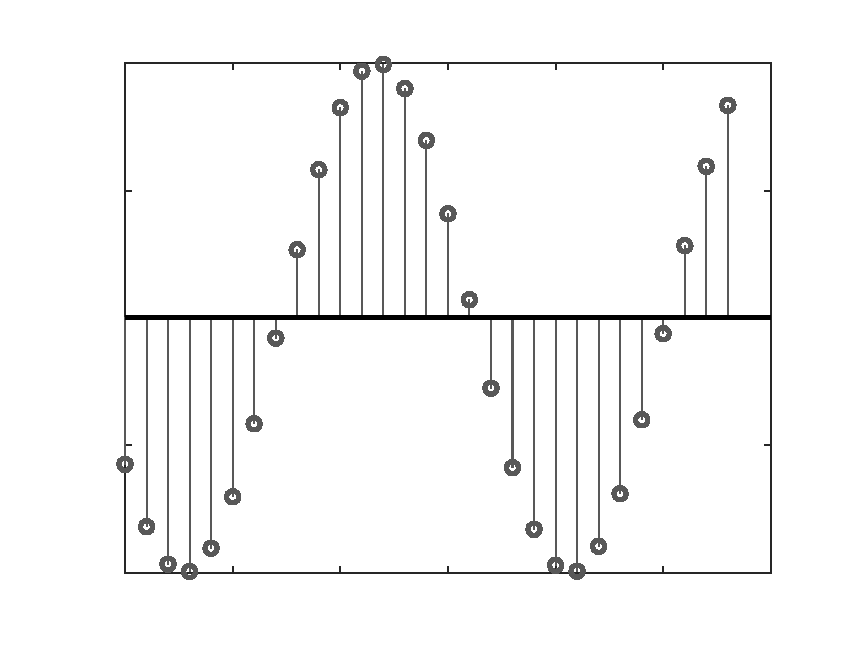
\includegraphics[scale=1]{octaves/stem-plot-inc}
\end{picture}%
\begin{picture}(400,300)(0,0)
\fontsize{6}{0}\selectfont\put(52,27.8){\makebox(0,0)[t]{\textcolor[rgb]{0.15,0.15,0.15}{{-10}}}}
\fontsize{6}{0}\selectfont\put(103.667,27.8){\makebox(0,0)[t]{\textcolor[rgb]{0.15,0.15,0.15}{{-5}}}}
\fontsize{6}{0}\selectfont\put(155.333,27.8){\makebox(0,0)[t]{\textcolor[rgb]{0.15,0.15,0.15}{{0}}}}
\fontsize{6}{0}\selectfont\put(207,27.8){\makebox(0,0)[t]{\textcolor[rgb]{0.15,0.15,0.15}{{5}}}}
\fontsize{6}{0}\selectfont\put(258.667,27.8){\makebox(0,0)[t]{\textcolor[rgb]{0.15,0.15,0.15}{{10}}}}
\fontsize{6}{0}\selectfont\put(310.333,27.8){\makebox(0,0)[t]{\textcolor[rgb]{0.15,0.15,0.15}{{15}}}}
\fontsize{6}{0}\selectfont\put(362,27.8){\makebox(0,0)[t]{\textcolor[rgb]{0.15,0.15,0.15}{{20}}}}
\fontsize{6}{0}\selectfont\put(48.5263,33){\makebox(0,0)[r]{\textcolor[rgb]{0.15,0.15,0.15}{{-1}}}}
\fontsize{6}{0}\selectfont\put(48.5263,94.125){\makebox(0,0)[r]{\textcolor[rgb]{0.15,0.15,0.15}{{-0.5}}}}
\fontsize{6}{0}\selectfont\put(48.5263,155.25){\makebox(0,0)[r]{\textcolor[rgb]{0.15,0.15,0.15}{{0}}}}
\fontsize{6}{0}\selectfont\put(48.5263,216.375){\makebox(0,0)[r]{\textcolor[rgb]{0.15,0.15,0.15}{{0.5}}}}
\fontsize{6}{0}\selectfont\put(48.5263,277.5){\makebox(0,0)[r]{\textcolor[rgb]{0.15,0.15,0.15}{{1}}}}
\fontsize{7}{0}\selectfont\put(207,287.5){\makebox(0,0)[b]{\textcolor[rgb]{0,0,0}{{A stem plot of a sinusoidal sequence}}}}
\end{picture}

}\caption{\emph{Stem plot} of a sinusoidal function. In particular, a stem plot of \texttt{cos(.35*x - .6)} has been performed with the help of the \texttt{octave} CLI. Pre-built binaries of the program are available at their website \texttt{https://octave.org/}.}\label{oct:stemPlot}
\end{center}
\end{figure}

Two kinds of digital signal representation exist. The first type is the common
digital signal where each sample is represented with a dot and a straight
line, while a \emph{boxedcar} signal will see each sample represented as a
straight line, in a similar fashion to the interpolation.

\subsubsection{Complex signals}

A signal can be either real or complex valued. A \emph{real se\-quen\-ce} comprises only real samples such that $x[i] \in \R, \forall i \in \Z$ while a \emph{complex se\-quen\-ce} has at least one complex sample $x[k] \in \C$. 
Complex se\-quen\-ces may be seen as the result of the sum of two, distinct, real se\-quen\-ces.
In particular, by writing \[\{x[n]\} = \{x_{re}[n]\} + j\{x_{im}[n]\}\] two different se\-quen\-ces, one for real part and the other one for the imaginary part, are summed together to form a single complex signal.
It's trivial to understand that a real valued signal can always be written as a complex signal if $x_{im}[n] \equiv 0, \forall n$. To do so, one can employ a so-called \textbf{Hilbert Transformer}, a specially crafted mathematical tool that is able to perform such an operation.

A complex signal's concise, alternative notation is \[\{x[n]\} = \{A[n]e^{-j\cdot f_t n}\},\] where the imaginary and real part are intrinsic in the complex exponential representation and can thus be obtained by decomposing it into a sine and a cosine addenda. The two representations are totally equivalent and are chosen for what they strive to represent. Real--and--imaginary parts notation highlights the two real and imaginary components of a signal, while the modulus--and--phase representation serves the purpose of making explicit the amplitude and the phase components of the very same sequence. The two are employed depending on the context and on the need.

\subsubsection{Length of a signal}

We have already seen that the values of the index $n$ can essentially lie between $-\infty$ to $\infty$. A signal can thus either be of \emph{finite} or \emph{infinite}-length. In the first case (and also typically) defined values for the se\-quen\-ce lay only in an interval $N_1 \leq n \leq N_2$, with $N_1 \leq N_2$ and both $-\infty < |N_1| \leq |N_2| < \infty$. The overall \emph{length} or \emph{duration} of the se\-quen\-ce will be $N = N_2 - N_1 + 1$. For instance, if the starting sample is at $3$ and the ending sample is at $7$, one has samples at $3, 4, 5, 6$ and $7$, leading to a total length or number of samples of $5$. Indeed, one could have obtained the same by applying the formula, that is $N = 7 - 3 + 1 = 4 + 1 = 5$. In the case of the infinite length se\-quen\-ce, the signal is defined for every value of $n \in \Z$, or after a certain $n_0$. For instance, $\{\cos{f_0 n}\}$ is an infinite-length se\-quen\-ce, because the signal ``never ends'', as there is no $n_1$ after which or before which the signal is null. Other infinite-length signals are any signal defined for all values after an $n_0 \in \Z$, or signals defined for all values before a certain index, the reverse case.

In practice, no real signal has infinite length. Still, it could be useful to think of signals as such to make them more mathematically treatable. Infinite-length signals, in fact, might pose less problems when manipulated with certain operations.

\subsubsection{Zero-padding}

A signal may see its length varied by arbitrary operations, or it must possess the same length of other sequences in order for some operations to be applied to it. A very common operation in that regard is to increase the length of a signal by appending or prepending $0$s to the signal, in a process called \textbf{zero-padding}. This usually involves a finite-length signal becoming an infinite-length signal by applying an infinitely long list of $0$s on both sides of the original signal; it is not uncommon, though, to apply the zero-padding technique to only one side of the signal. Another way to handle zero-padding is to simply add a finite---yet necessary for specific needs---number of $0$s depending on the duty to perform. For instance, let's simply think of the simple sum of two sequences, with different length. To add two signals of different length, padding the shorter sequence is mandatory in order to perform a meaningful operation.

\subsubsection{Causality}
A se\-quen\-ce is said to be \emph{right-sided} if it has zero-valued samples or no samples for each $n < N_1$. A special case of right-sided se\-quen\-ce is when $N_1 \geq 0$, the case of a \textbf{causal} signal.

Vice-versa, a se\-quen\-ce is said to be \emph{left-sided} if it has zero-valued samples or no samples for each $n > N_2$. The same way, when a left-sided se\-quen\-ce has $N_2 \leq 0$, we are in the case of an \textbf{anti-causal} signal.

Basically, right-sided signals are all signals that ``are relevant only \emph{after} a certain time $N_1$'', and left-sided signals are all signals that ``are relevant \emph{before} a given time $N_2$''. A similar circumstance can be said concerning causal and anti-causal signals, but with $N_1=N_2=0$.

\subsubsection{Strength of a signal and signal comparison}

An important concept is the \textbf{strength} of a signal, also called \emph{size} of a signal. The strength of a signal is the $\mathcal{L}_p$-norm of the se\-quen\-ce,
\[
||x||_p = \left(\sum_{i=N_1}^{N_2} |x[n]|^p\right)^{\frac{1}{p}},
\]
where $p \in \N \setminus \{0\}$ is a positive integer different from zero. In the strength definition, one cannot ignore the specific value of the parameter $p$, which essentially determines the kind of operation which is involved to compute the strength value. Typically, one has $p=1,2,\infty$, with $p=2$ being the \emph{root mean squares} apart from a scaling factor---in fact, RMS is the square root of the \textbf{mean} of the squares and not simply the square root of the sum of the squares, so there's an additional $\frac{1}{\sqrt{N}}$ factor that the $2$-strength lacks, with $N$ length of the sequence. The other two routine cases are $p=1$ corresponding to the \emph{mean absolute value} of the signal---except for a constant scaling factor---and $p=\infty$ where the strength of the signal would be the \emph{absolute peak value} of the signal. Choosing a peculiar $p$, in essence, gives a different meaning to the strength of a signal.

We can use the above tool to compute in some way the difference between two sequences; from the concept of signal strength, the concept of \emph{relative error} immediately arises.
Let $\{y[n]\}, 0 \leq n \leq N - 1$ be an approximation of the signal $\{x[n]\}, 0 \leq n \leq N - 1$, both being causal sequences having the same length.
In this case, one calls \textbf{relative error} the quantity
\begin{equation}\label{eqn:RelativeError}
	E_{rel} = \left(\frac{\sum_{n=0}^{N-1} |y[n] - x[n]|^2}{\sum_{n=0}^{N-1} |x[n]|^2}\right)^\frac{1}{2},
\end{equation}
the ratio of the $\mathcal L_2$-norm of the signal which is the difference between $y[n]$ and $x[n]$, and the $\mathcal L_2$-norm of the signal $\{x[n]\}$ alone. The relative error between a sequence $y$ and a sequence $x$ is actually the $2$-strength of the difference between $y$ and $x$ across their length from sample $0$ to sample $N-1$, divided by the $2$-strength of the sequence $x$. Everything is square-rooted, as each $2$-norm is actually square-rooted from its definition.

The numerator of such quantity can be considered as the error between se\-quen\-ces $x$ and $y$, while the denominator is the $2$-strength of a non-approximated se\-quen\-ce. We can interpret it as the ratio between a kind of `error' of the sequences $y$ and $x$, measured through the $\mathcal L_2$-norm, and the overall $2$-strength of the sequence~$x$.

\subsection{Operations on se\-quen\-ces}\label{sec:operationsOnSequences}

Se\-quen\-ces may be subject to \emph{operations}. In particular, operations can be described by directed graphs in which there are (possibly multiple) input se\-quen\-ces and (possibly multiple) output se\-quen\-ces resulting from the operation. Of course, there may be well more than one input and one output. Operations in general can be seen as \textbf{discrete-time systems} as they allow manipulation of discrete-time sequences.

    \begin{figure}[ht]
\begin{center}
\begin{tikzpicture}

    \node                 (input)                                 {$\{x[n]\}$};
    \node[squarednode]    (operation)     [right=of input]        {Operation};
    \node                 (output)        [right=of operation]    {$\{y[n]\}$};

    \draw[->] (input.east) -- (operation.west);
    \draw[->] (operation.east) -- (output.west);
\end{tikzpicture}\caption{The general scheme for elementary operations.}\label{tikz:operation-scheme}
\end{center}
\end{figure}

Basic signal operations are called \textbf{elementary operations}. The first elementary operation is the \emph{modulation}, an operation in which a signal $x$ is multiplied by another signal, say $w$, to produce an output signal $y$ such that $$y[n] = x[n]\cdot w[n].$$ A common application of the modulation is the \textbf{windowing} process, in which an infinite-length signal $x$ is ``windowed'' by a finite-length signal $w$, whose non-zero values are limited to a finite interval and the non-zero values are all equal to $1$. In that case, it would be like ``selecting'' the values of $x$ that lay in the $w$ window, as any other value would be multiplied by $0$. Modulation is denoted with a cross inside a circle, as shown in Diagram~\ref{tikz:modulation-operation}.

\begin{figure}[ht]
\begin{center}
    \begin{tikzpicture}
    \node [](A){$x[n]$};
    \node [draw, fill=purple!15,circle,crossp, thick,minimum width=0.5 cm](B) at (1,0){};
    \node [](C) at(2,0){$y[n]$};
    \node [](D) at(1,-1){$w[n]$};
    \draw[->] (A) -- (B);
    \draw[->] (B) -- (C);
    \draw[->] (D) -- (B);
\end{tikzpicture}\caption{Notation for the modulation (product) operation.}\label{tikz:modulation-operation}
\end{center}
\end{figure}

Other elementary operations are the \emph{multiplication} operation and the \emph{addition} operation. The multiplier is denoted by a triangle---a triangle-like symbol is adopted---while the addition is a plus symbol inside a circle. Diagrams~\ref{tikz:multiplication-operation} and~\ref{tikz:addition-operation} summarize the overall notation. This time, multiplication is not performed between entire signals, but instead a constant $A$ multiplies a signal $x$, such that $$y[n] = A \cdot x[n].$$ Essentially, a multiplication is equivalent with a modulation of a signal $x$ with another signal $A$, which is of the same length and of constant value. The addition is instead performed between two distinct signals, hence $$z[n] = x[n] + y[n].$$ 

\begin{figure}[ht]
\begin{center}
    \begin{tikzpicture}
    \node [](A){$x[n]$};
    \node [draw, fill=red!10,isosceles triangle,thick,minimum width=.4 cm](B) at (1.5,0){$A$};
    \node [](C) at(3,0){$y[n]$};
    \draw[->] (A) -- (B);
    \draw[->] (B) -- (C);
\end{tikzpicture}\caption{Notation for the multiplication (product for a constant $A$) operation.}\label{tikz:multiplication-operation}
\end{center}
\end{figure}

\begin{figure}[ht]
\begin{center}
\begin{tikzpicture}
    \node [](A) at (0,0){$x[n]$};
    \node [draw, fill=green!15,circle,plus,thick,minimum width=.5 cm](B) at (1,0){};
    \node [](C) at(2,0){$z[n]$};
    \node [](D) at(1,-1){$y[n]$};
    \draw[->] (A) -- (B);
    \draw[->] (B) -- (C);
    \draw[->] (D) -- (B);
\end{tikzpicture}\caption{Notation for the addition (sum) operation.}\label{tikz:addition-operation}
\end{center}
\end{figure}

Much relevant elementary operations are, indeed, the \emph{time delay} and
\emph{time advance}. A signal that is time-delayed is a signal which is a copy
of the original signal, but translated in time (delayed in this case).
Vice-versa, in the case of time advance, the signal copy of the original will be
anticipated. In the first case, the adopted symbol is $z^{-1}$, while for the
anticipation it is $z$. The reason why the anticipation and the delay symbols involve a $z$ letter will be clear from chapter~\ref{sec:zTransform}. Hence, $y[n] = x[n - 1]$ in the case of the delay and $y[n] = x[n + 1]$ in the case of the anticipation.

\begin{figure}[ht]
\begin{center}
    \begin{tikzpicture}
    \node [](A){$x[n]$};
    \node [draw, fill=red!10,boxfilter](B) at (1.5,0){$z^{-1}$};
    \node [](C) at(3,0){$x[n-1]$};
    \draw[->] (A) -- (B);
    \draw[->] (B) -- (C);
\end{tikzpicture}\caption{Notation for the time delaying operation.}\label{tikz:delaying-operation}
\end{center}
\end{figure}

\begin{figure}[ht]
\begin{center}
    \begin{tikzpicture}
    \node [](A){$x[n]$};
    \node [draw, fill=red!10,rectangle,thick,minimum width=.7 cm, minimum height=.5cm](B) at (1.5,0){$z$};
    \node [](C) at(3,0){$x[n+1]$};
    \draw[->] (A) -- (B);
    \draw[->] (B) -- (C);
\end{tikzpicture}\caption{Notation for the time advance operation.}\label{tikz:advance-operation}
\end{center}
\end{figure}

An interesting operation is the \emph{time reversal} or \emph{folding}. The folding operation inverts the time axis of a signal, that means $y[n] = x[-n]$. Any sample that was located on the positive axis is now ``reflected'' on the negative axis, and vice-versa. Time reversal does not have any explicit symbol, since it is an operation that requires a complete reflection of a signal from its origin point and should be handled carefully. In particular, performing such operation requires to first collect the entire signal, as all output samples in the past should be collected from the future original signal.

Yet another common `operation' is the \emph{branching} operation, in which a signal $w$ is simply the copy of the input signal, as well as the $y$ signal (a single input is copied into two outputs). Branching allows signals to flow into multiple blocks by copying it. Branching is shown in Diagram~\ref{tikz:branchingOperation}.
\begin{figure}[ht]
\begin{center}
    \begin{tikzpicture}
    \node [](A){$x[n]$};
    \node [draw, fill=black!100,inner sep=1pt,circle,label=above:{b}](B) at (1.5,0){};
    \node [](C) at(3,0){$x[n]$};
    \node [](D) at(1.5,-1.5){$x[n]$};
    \draw[->] (A) -- (B) -- (C);
    \draw[->] (B) -- (D);
\end{tikzpicture}\caption{Notation for the branching (signal splitting) operation. The $b$ node allows splitting of the signal into two equal branches where $x$ is routed.}\label{tikz:branchingOperation}
\end{center}
\end{figure}

In order to apply most of the above operations, two signals should possess the same length---in those cases where this does not occur, a \emph{zero-padding} is required. For instance, to perform addition on two signals, the two signals must share the same length, therefore it is mandatory to at least perform a zero-padding on the shortest of the signals. Where a zero-padding was necessary, the sum will simply leave the longer sequence unalterated. Still, infinitely long signals can be virtually summed together by summing up all infinite samples.

Multiple elementary operations can be combined as well, by building a directed graph in which the signals are subject to multiple eventual operations, in the order determined by the particular graph. Usually, multiple operations should be necessary and are therefore applied in special manners to obtain the desired result.

\section{Ensemble Averaging}

A very powerful---although non elementary---operation to apply to a signal is the \textbf{ensemble averaging}. Ensemble averaging is the operation of performing an average of a signal when multiple, independent measures are available. The goal of the ensemble averaging is to enhance the quality of a signal with respect to a noise which affects it. In other words, the result is expected to suffer less from noise than the original signal.

Suppose $i$-th measured signal $x_i$ has two components $x_i = s + d_i$, the
first one relative to an original signal $s$ and the noise component $d_i$, which
varies according to the measurement. Each measurement will measure the same signal $s$, but carry its own noise $d_i$. The ensemble average of the $K$ measurements is the signal $x_{avg}$ built from the mean of $K$ measurements of $s + d$,
\begin{equation}\label{eqn:EnsambleAveraging}
	x_{avg} = \frac{1}{K}\sum_{i=1}^{K} (s + d_i) = s + \frac{1}{K}\sum_{i=1}^{K}d_i,
\end{equation}
which tends to the original signal $s$ as the number of signals $K \rightarrow \infty$ approaches infinity. The benefit of the ensemble averaging lies in the fact that \emph{the variance of the white noise $d_i$ is reduced by a factor of $K$ and by the averaging process}, leading to a much more reasonable replica of the original signal $s$, having noise of reduced variance. Error variance will approximately be $\frac 1 K$-th of the original noise variance, a reduction of---indeed---a factor of $K$. An example of application of ensemble averaging is shown in Figure~\ref{oct:ensembleAveraging}.

On the chart, the ensemble averaging is a powerful method to remove the noise, having many different recordings of a signal at our disposal.
The common noise encountered, though, will hardly be a noise such that their average is zero---moreover, a typical noise will hardly be white and completely uncorrelated with the original signal $s$.
For these reasons, this method is not perfect and manifests some drawbacks. Nevertheless, the method works and the effects are palpable, even if the noise does not comply with our hypothesis.

\begin{figure*}[ht]
\begin{center}
\scalebox{0.32}{
% Title: gl2ps_renderer figure
% Creator: GL2PS 1.4.2, (C) 1999-2020 C. Geuzaine
% For: Octave
% CreationDate: Wed Oct 19 09:01:13 2022
\setlength{\unitlength}{1pt}
\begin{picture}(0,0)
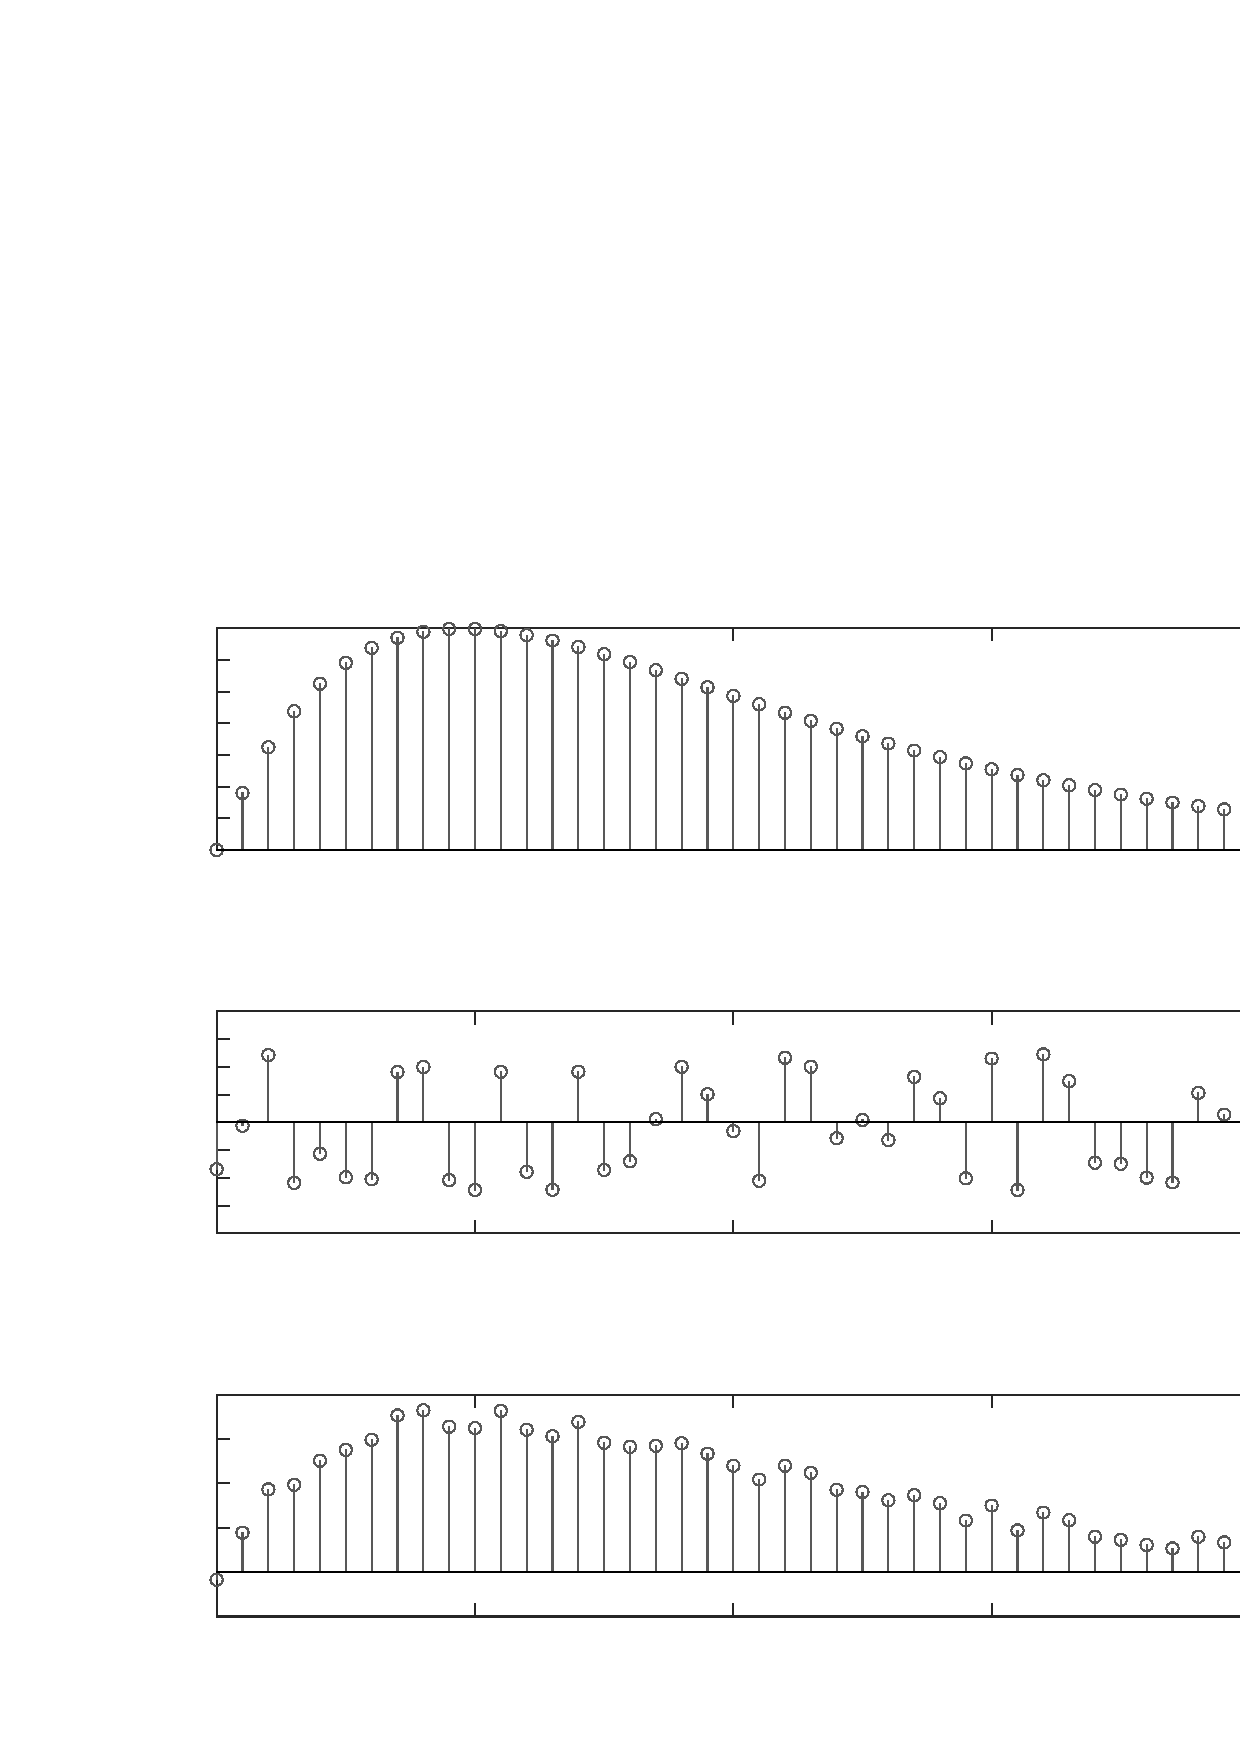
\includegraphics[scale=1]{octaves/ensembleAveraging-inc}
\end{picture}%
\begin{picture}(800,600)(0,0)
\fontsize{13}{0}\selectfont\put(104,423.523){\makebox(0,0)[t]{\textcolor[rgb]{0.15,0.15,0.15}{{0}}}}
\fontsize{13}{0}\selectfont\put(228,423.523){\makebox(0,0)[t]{\textcolor[rgb]{0.15,0.15,0.15}{{10}}}}
\fontsize{13}{0}\selectfont\put(352,423.523){\makebox(0,0)[t]{\textcolor[rgb]{0.15,0.15,0.15}{{20}}}}
\fontsize{13}{0}\selectfont\put(476,423.523){\makebox(0,0)[t]{\textcolor[rgb]{0.15,0.15,0.15}{{30}}}}
\fontsize{13}{0}\selectfont\put(600,423.523){\makebox(0,0)[t]{\textcolor[rgb]{0.15,0.15,0.15}{{40}}}}
\fontsize{13}{0}\selectfont\put(724,423.523){\makebox(0,0)[t]{\textcolor[rgb]{0.15,0.15,0.15}{{50}}}}
\fontsize{13}{0}\selectfont\put(97.0525,433.898){\makebox(0,0)[r]{\textcolor[rgb]{0.15,0.15,0.15}{{0}}}}
\fontsize{13}{0}\selectfont\put(97.0525,449.116){\makebox(0,0)[r]{\textcolor[rgb]{0.15,0.15,0.15}{{1}}}}
\fontsize{13}{0}\selectfont\put(97.0525,464.334){\makebox(0,0)[r]{\textcolor[rgb]{0.15,0.15,0.15}{{2}}}}
\fontsize{13}{0}\selectfont\put(97.0525,479.552){\makebox(0,0)[r]{\textcolor[rgb]{0.15,0.15,0.15}{{3}}}}
\fontsize{13}{0}\selectfont\put(97.0525,494.77){\makebox(0,0)[r]{\textcolor[rgb]{0.15,0.15,0.15}{{4}}}}
\fontsize{13}{0}\selectfont\put(97.0525,509.988){\makebox(0,0)[r]{\textcolor[rgb]{0.15,0.15,0.15}{{5}}}}
\fontsize{13}{0}\selectfont\put(97.0525,525.206){\makebox(0,0)[r]{\textcolor[rgb]{0.15,0.15,0.15}{{6}}}}
\fontsize{13}{0}\selectfont\put(97.0525,540.424){\makebox(0,0)[r]{\textcolor[rgb]{0.15,0.15,0.15}{{7}}}}
\fontsize{15}{0}\selectfont\put(414,550.424){\makebox(0,0)[b]{\textcolor[rgb]{0,0,0}{{Original uncorrupted sequence}}}}
\fontsize{15}{0}\selectfont\put(84.0526,487.161){\rotatebox{90}{\makebox(0,0)[b]{\textcolor[rgb]{0.15,0.15,0.15}{{Amplitude}}}}}
\fontsize{15}{0}\selectfont\put(414,407.523){\makebox(0,0)[t]{\textcolor[rgb]{0.15,0.15,0.15}{{Time index n}}}}
\fontsize{13}{0}\selectfont\put(104,239.574){\makebox(0,0)[t]{\textcolor[rgb]{0.15,0.15,0.15}{{0}}}}
\fontsize{13}{0}\selectfont\put(228,239.574){\makebox(0,0)[t]{\textcolor[rgb]{0.15,0.15,0.15}{{10}}}}
\fontsize{13}{0}\selectfont\put(352,239.574){\makebox(0,0)[t]{\textcolor[rgb]{0.15,0.15,0.15}{{20}}}}
\fontsize{13}{0}\selectfont\put(476,239.574){\makebox(0,0)[t]{\textcolor[rgb]{0.15,0.15,0.15}{{30}}}}
\fontsize{13}{0}\selectfont\put(600,239.574){\makebox(0,0)[t]{\textcolor[rgb]{0.15,0.15,0.15}{{40}}}}
\fontsize{13}{0}\selectfont\put(724,239.574){\makebox(0,0)[t]{\textcolor[rgb]{0.15,0.15,0.15}{{50}}}}
\fontsize{13}{0}\selectfont\put(97.0525,249.949){\makebox(0,0)[r]{\textcolor[rgb]{0.15,0.15,0.15}{{-0.8}}}}
\fontsize{13}{0}\selectfont\put(97.0525,263.265){\makebox(0,0)[r]{\textcolor[rgb]{0.15,0.15,0.15}{{-0.6}}}}
\fontsize{13}{0}\selectfont\put(97.0525,276.58){\makebox(0,0)[r]{\textcolor[rgb]{0.15,0.15,0.15}{{-0.4}}}}
\fontsize{13}{0}\selectfont\put(97.0525,289.896){\makebox(0,0)[r]{\textcolor[rgb]{0.15,0.15,0.15}{{-0.2}}}}
\fontsize{13}{0}\selectfont\put(97.0525,303.212){\makebox(0,0)[r]{\textcolor[rgb]{0.15,0.15,0.15}{{0}}}}
\fontsize{13}{0}\selectfont\put(97.0525,316.527){\makebox(0,0)[r]{\textcolor[rgb]{0.15,0.15,0.15}{{0.2}}}}
\fontsize{13}{0}\selectfont\put(97.0525,329.843){\makebox(0,0)[r]{\textcolor[rgb]{0.15,0.15,0.15}{{0.4}}}}
\fontsize{13}{0}\selectfont\put(97.0525,343.159){\makebox(0,0)[r]{\textcolor[rgb]{0.15,0.15,0.15}{{0.6}}}}
\fontsize{13}{0}\selectfont\put(97.0525,356.475){\makebox(0,0)[r]{\textcolor[rgb]{0.15,0.15,0.15}{{0.8}}}}
\fontsize{15}{0}\selectfont\put(414,366.475){\makebox(0,0)[b]{\textcolor[rgb]{0,0,0}{{Noise}}}}
\fontsize{15}{0}\selectfont\put(68.0525,303.212){\rotatebox{90}{\makebox(0,0)[b]{\textcolor[rgb]{0.15,0.15,0.15}{{Amplitude}}}}}
\fontsize{15}{0}\selectfont\put(414,223.574){\makebox(0,0)[t]{\textcolor[rgb]{0.15,0.15,0.15}{{Time index n}}}}
\fontsize{13}{0}\selectfont\put(104,55.625){\makebox(0,0)[t]{\textcolor[rgb]{0.15,0.15,0.15}{{0}}}}
\fontsize{13}{0}\selectfont\put(228,55.625){\makebox(0,0)[t]{\textcolor[rgb]{0.15,0.15,0.15}{{10}}}}
\fontsize{13}{0}\selectfont\put(352,55.625){\makebox(0,0)[t]{\textcolor[rgb]{0.15,0.15,0.15}{{20}}}}
\fontsize{13}{0}\selectfont\put(476,55.625){\makebox(0,0)[t]{\textcolor[rgb]{0.15,0.15,0.15}{{30}}}}
\fontsize{13}{0}\selectfont\put(600,55.625){\makebox(0,0)[t]{\textcolor[rgb]{0.15,0.15,0.15}{{40}}}}
\fontsize{13}{0}\selectfont\put(724,55.625){\makebox(0,0)[t]{\textcolor[rgb]{0.15,0.15,0.15}{{50}}}}
\fontsize{13}{0}\selectfont\put(97.0525,66){\makebox(0,0)[r]{\textcolor[rgb]{0.15,0.15,0.15}{{-2}}}}
\fontsize{13}{0}\selectfont\put(97.0525,87.3051){\makebox(0,0)[r]{\textcolor[rgb]{0.15,0.15,0.15}{{0}}}}
\fontsize{13}{0}\selectfont\put(97.0525,108.61){\makebox(0,0)[r]{\textcolor[rgb]{0.15,0.15,0.15}{{2}}}}
\fontsize{13}{0}\selectfont\put(97.0525,129.915){\makebox(0,0)[r]{\textcolor[rgb]{0.15,0.15,0.15}{{4}}}}
\fontsize{13}{0}\selectfont\put(97.0525,151.22){\makebox(0,0)[r]{\textcolor[rgb]{0.15,0.15,0.15}{{6}}}}
\fontsize{13}{0}\selectfont\put(97.0525,172.525){\makebox(0,0)[r]{\textcolor[rgb]{0.15,0.15,0.15}{{8}}}}
\fontsize{15}{0}\selectfont\put(414,182.525){\makebox(0,0)[b]{\textcolor[rgb]{0,0,0}{{Corrupted sequence}}}}
\fontsize{15}{0}\selectfont\put(79.0526,119.263){\rotatebox{90}{\makebox(0,0)[b]{\textcolor[rgb]{0.15,0.15,0.15}{{Amplitude}}}}}
\fontsize{15}{0}\selectfont\put(414,39.6249){\makebox(0,0)[t]{\textcolor[rgb]{0.15,0.15,0.15}{{Time index n}}}}
\end{picture}

% Title: gl2ps_renderer figure
% Creator: GL2PS 1.4.2, (C) 1999-2020 C. Geuzaine
% For: Octave
% CreationDate: Wed Oct 19 09:02:39 2022
\setlength{\unitlength}{1pt}
\begin{picture}(0,0)
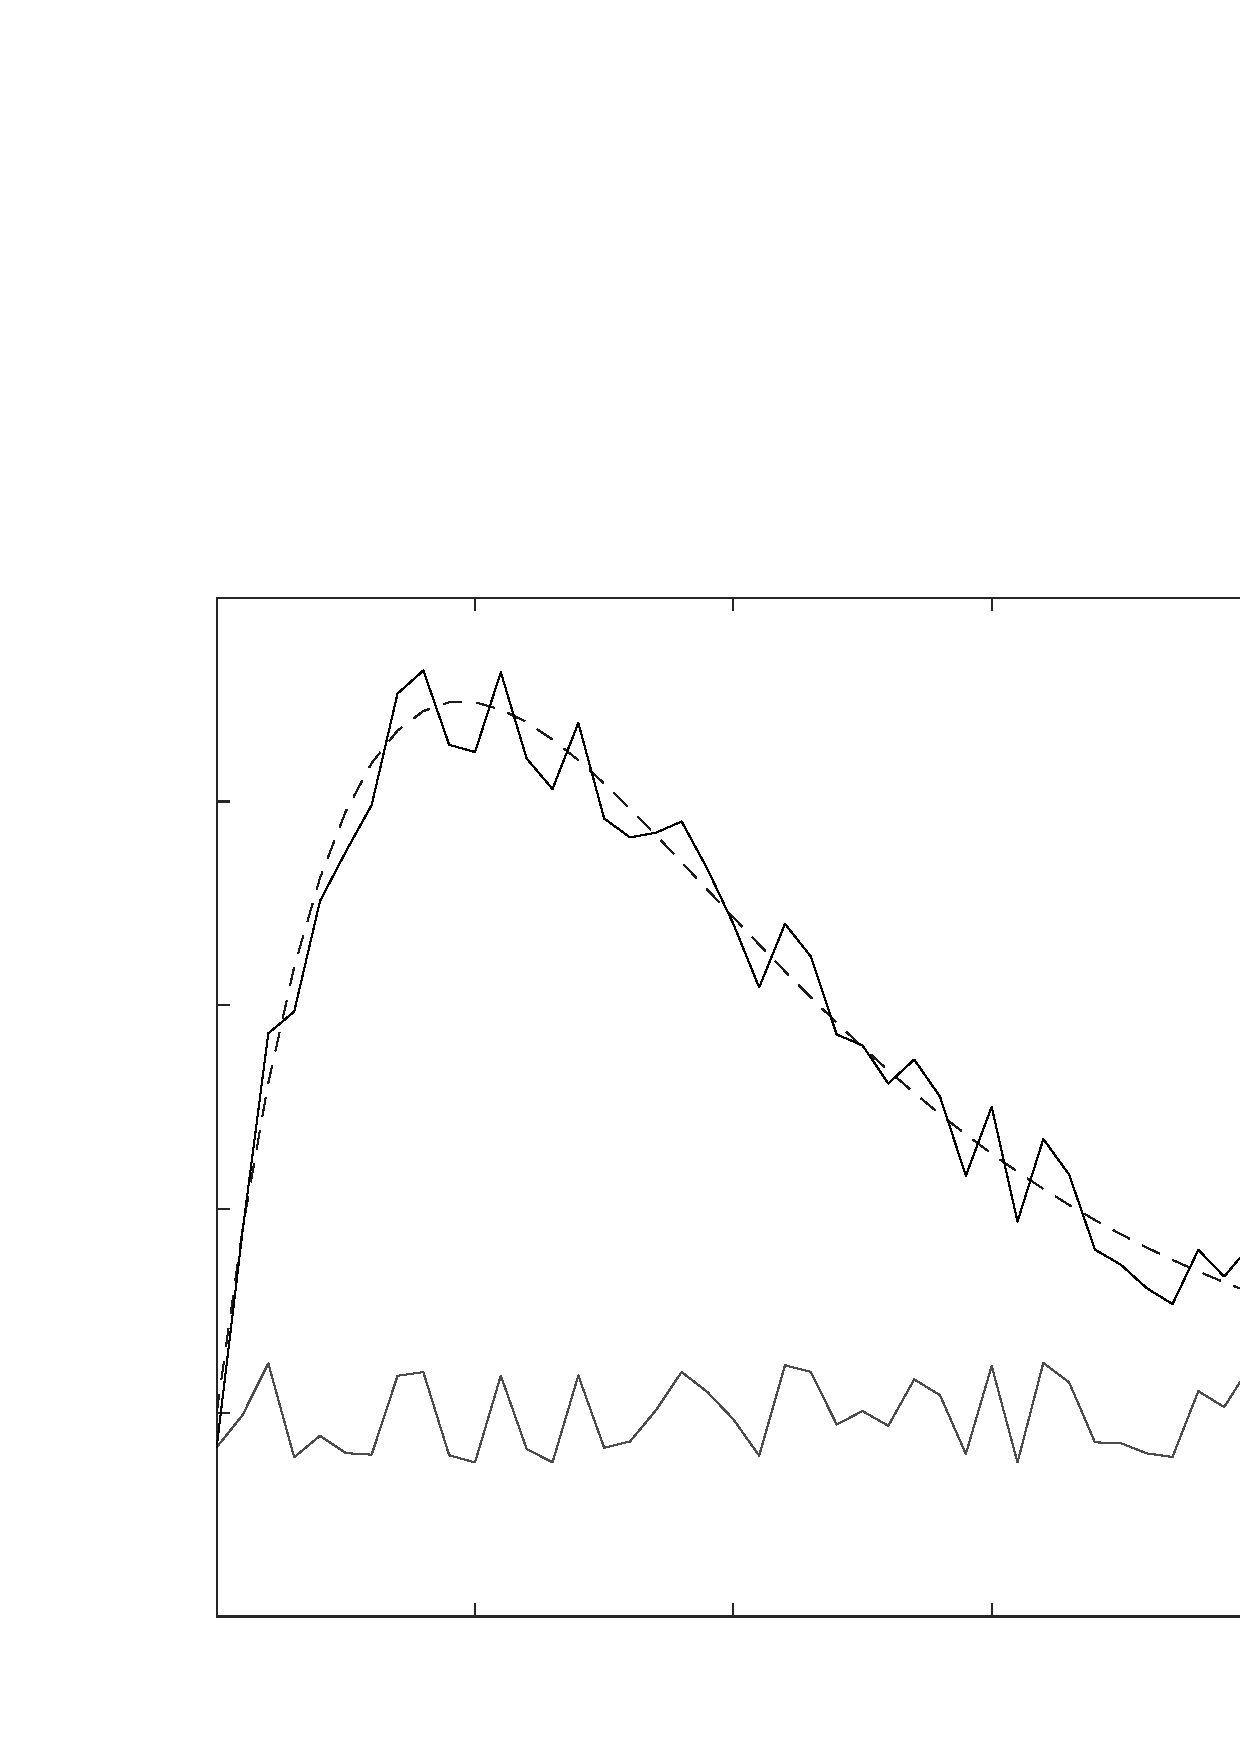
\includegraphics[scale=1]{octaves/ensembleAveragingTwo-inc}
\end{picture}%
\begin{picture}(800,600)(0,0)
\fontsize{13}{0}\selectfont\put(104,55.5788){\makebox(0,0)[t]{\textcolor[rgb]{0.15,0.15,0.15}{{0}}}}
\fontsize{13}{0}\selectfont\put(228,55.5788){\makebox(0,0)[t]{\textcolor[rgb]{0.15,0.15,0.15}{{10}}}}
\fontsize{13}{0}\selectfont\put(352,55.5788){\makebox(0,0)[t]{\textcolor[rgb]{0.15,0.15,0.15}{{20}}}}
\fontsize{13}{0}\selectfont\put(476,55.5788){\makebox(0,0)[t]{\textcolor[rgb]{0.15,0.15,0.15}{{30}}}}
\fontsize{13}{0}\selectfont\put(600,55.5788){\makebox(0,0)[t]{\textcolor[rgb]{0.15,0.15,0.15}{{40}}}}
\fontsize{13}{0}\selectfont\put(724,55.5788){\makebox(0,0)[t]{\textcolor[rgb]{0.15,0.15,0.15}{{50}}}}
\fontsize{13}{0}\selectfont\put(97.0525,66){\makebox(0,0)[r]{\textcolor[rgb]{0.15,0.15,0.15}{{-2}}}}
\fontsize{13}{0}\selectfont\put(97.0525,163.8){\makebox(0,0)[r]{\textcolor[rgb]{0.15,0.15,0.15}{{0}}}}
\fontsize{13}{0}\selectfont\put(97.0525,261.6){\makebox(0,0)[r]{\textcolor[rgb]{0.15,0.15,0.15}{{2}}}}
\fontsize{13}{0}\selectfont\put(97.0525,359.4){\makebox(0,0)[r]{\textcolor[rgb]{0.15,0.15,0.15}{{4}}}}
\fontsize{13}{0}\selectfont\put(97.0525,457.2){\makebox(0,0)[r]{\textcolor[rgb]{0.15,0.15,0.15}{{6}}}}
\fontsize{13}{0}\selectfont\put(97.0525,555){\makebox(0,0)[r]{\textcolor[rgb]{0.15,0.15,0.15}{{8}}}}
\fontsize{15}{0}\selectfont\put(414,39.5788){\makebox(0,0)[t]{\textcolor[rgb]{0.15,0.15,0.15}{{Time index n}}}}
\fontsize{15}{0}\selectfont\put(79.0526,310.5){\rotatebox{90}{\makebox(0,0)[b]{\textcolor[rgb]{0.15,0.15,0.15}{{Amplitude}}}}}
\fontsize{12}{0}\selectfont\put(693.005,536.005){\makebox(0,0)[l]{\textcolor[rgb]{0,0,0}{{x[n]}}}}
\fontsize{12}{0}\selectfont\put(693.005,518.007){\makebox(0,0)[l]{\textcolor[rgb]{0,0,0}{{y[n]}}}}
\end{picture}

}\caption{The ensemble averaging. On the left, the original uncorrupted sequence $s[n]$, the noise $d[n]$ and the corrupted sequence $x[n]$. On the right, the dashed line represents the sequence $y[n]$, a ``recovered'' version of the original sequence $s[n]$. Recovering has been performed by means of the ensemble averaging process. The noise has been generated by means of a random noise generator---although it tries to best create a random white gaussian noise, on practice this is impossible since it would require an infinite amount of samples to store it. However, longer randomly-generated sequences might exhibit much more similar behaviors with respect to a true average white noises.}\label{oct:ensembleAveraging}
\end{center}
\end{figure*}

\section{Sample Rate Alteration}

The operation of alterating the sample rate $F_S$ is much important. Generally, it is adopted to obtain a new signal $x'$ from a signal $x$, but with a different sample rate $F'_S$. The new sample rate can either be high\-er or lower than the original signal, so that a \emph{sampling rate alteration ratio} can be defined,
\begin{equation}\label{eqn:SamplingRateAlterationRatio}
	R_S = \frac{F'_S}{F_S}.
\end{equation}

The ratio in equation \ref{eqn:SamplingRateAlterationRatio} can either be greater or lower than $1$, and determines the nature of the sample rate alteration. In particolar, in the case of $R_S > 1$ one performs the \textbf{interpolation} operation, while in the opposite case of $R_S < 1$ one gets the \textbf{decimation} operation.

Two operations are imperative for, respectively, interpolation and decimation: the \emph{up-sampling} and the \emph{down-sam\-pling} operations. To be specific, in order to perform interpolation a \emph{further} operation is needed other than up-sampling.

\subsubsection{Up-Sampling}

The up-sampling operation by an integer factor $L > 1$ involves the addition of
$L-1$ zero-valued samples inserted in between two consecutive samples of the
original signal:

\begin{equation}\label{eqn:UpSampling}
	x_u[n] =
	\left\{
		\begin{array}{ll}
			x[n/L] 	& n=0,\pm L, \pm 2L, \dots \\
			0 	& otherwise
		\end{array}
	\right.
\end{equation}

Such definition means that the output sequence will be composed of zeros, except at those samples at which $n$ is a multiple of the interpolation factor $L$.

Up-sampling operation is denoted by a $\uparrow L$ block, as in Diagram~\ref{tikz:upsamplingOperation}. Upsampling is usually followed by \emph{interpolation} to produce an actually meaningful signal.

\begin{figure}[ht]
\begin{center}
    \begin{tikzpicture}
    \node [](A){$x[n]$};
    \node [draw,rectangle,thick](B) at (1.5,0){$\uparrow L$};
    \node [](C) at(3,0){$x_u[n]$};
    \draw[->] (A) -- (B) -- (C);
\end{tikzpicture}\caption{Notation for the up-sampling operation by a factor $L$.}\label{tikz:upsamplingOperation}
\end{center}
\end{figure}

On its essential core, up-sampling is an \emph{uphill} transformation that involves taking a signal over a discrete-time domain with sampling rate $\frac 1 T$ and generating a new signal with an higher sampling rate $\frac 1 {NT}$ by means of a convolution with a delta impulse in the output domain. Such a delta impulse will correspond to a train of delta impulses with the new, desired, sampling rate frequency. The convolution with the correct delta impulses will yield a new signal, having the same original values, plus the new zeros added between the previous values.

\subsubsection{Down-Sampling}

The down-sampling operation by an integer factor $M > 1$ means that from the
original signal only one sample every $M$ is preserved. This way, $M-1$ consecutive
in between samples are removed from the signal, while a single one every $M$ samples is preserved,
\begin{equation}\label{eqn:DownSampling}
	x_d[n] = x[nM]
\end{equation}

Down-sampling operation is denoted by a $\downarrow M$ block, as in Figure~\ref{tikz:downsamplingOperation}.
\begin{figure}[ht]
\begin{center}
    \begin{tikzpicture}
    \node [](A){$x[n]$};
    \node [draw,rectangle,thick](B) at (1.5,0){$\downarrow M$};
    \node [](C) at(3,0){$x_u[n]$};
    \draw[->] (A) -- (B) -- (C);
\end{tikzpicture}\caption{Notation for the down-sampling operation by a factor $M$.}\label{tikz:downsamplingOperation}
\end{center}
\end{figure}
The result of downsampling is a se\-quen\-ce in which some values are missing, those that are removed by the downsampling operation. A crucial risk of downsampling that we will tackle later on is the \textbf{aliasing} phenomenon.
\begin{figure*}[ht]
    \centering
    \scalebox{0.6}{
    % Title: gl2ps_renderer figure
% Creator: GL2PS 1.4.2, (C) 1999-2020 C. Geuzaine
% For: Octave
% CreationDate: Wed Oct 19 09:18:32 2022
\setlength{\unitlength}{1pt}
\begin{picture}(0,0)
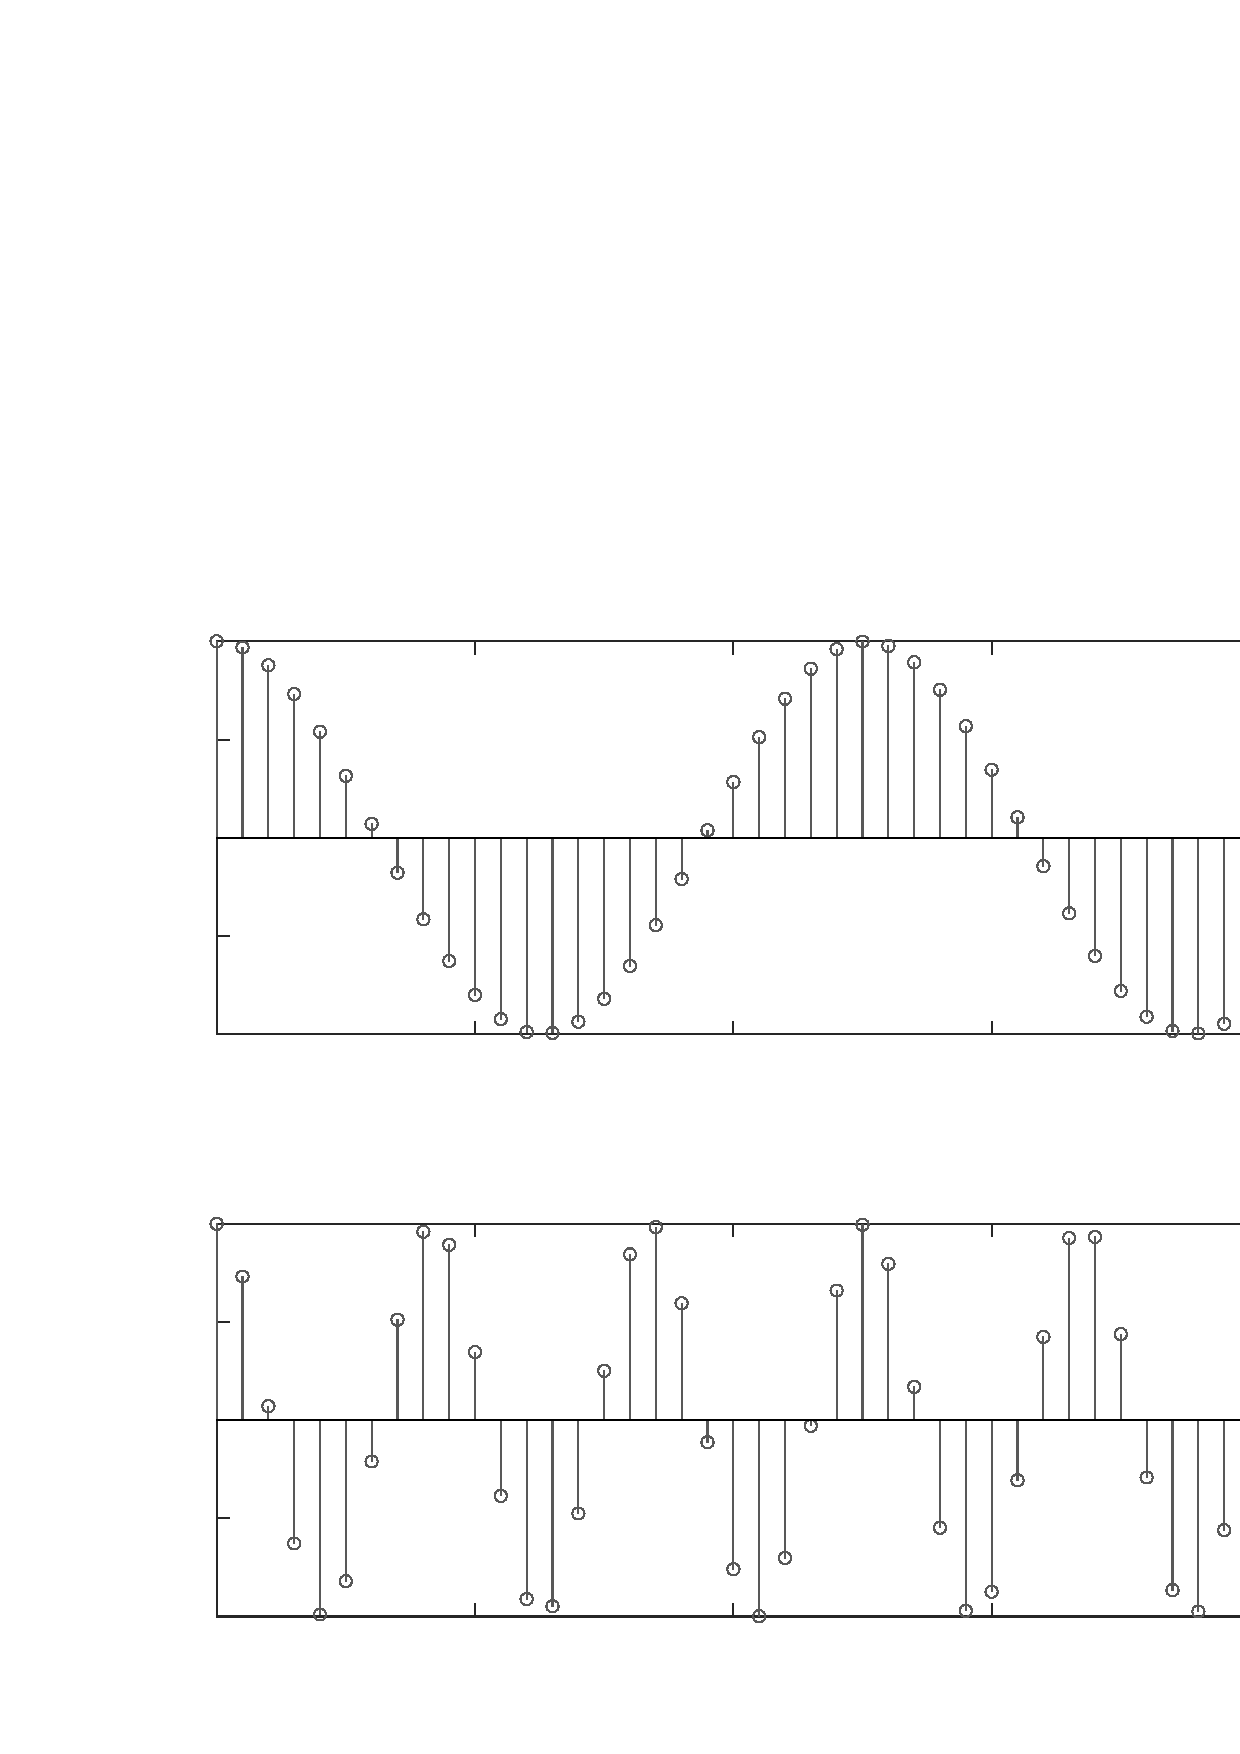
\includegraphics[scale=1]{octaves/downsamplingOperationEffect-inc}
\end{picture}%
\begin{picture}(800,600)(0,0)
\fontsize{13}{0}\selectfont\put(104,335.117){\makebox(0,0)[t]{\textcolor[rgb]{0.15,0.15,0.15}{{0}}}}
\fontsize{13}{0}\selectfont\put(228,335.117){\makebox(0,0)[t]{\textcolor[rgb]{0.15,0.15,0.15}{{10}}}}
\fontsize{13}{0}\selectfont\put(352,335.117){\makebox(0,0)[t]{\textcolor[rgb]{0.15,0.15,0.15}{{20}}}}
\fontsize{13}{0}\selectfont\put(476,335.117){\makebox(0,0)[t]{\textcolor[rgb]{0.15,0.15,0.15}{{30}}}}
\fontsize{13}{0}\selectfont\put(600,335.117){\makebox(0,0)[t]{\textcolor[rgb]{0.15,0.15,0.15}{{40}}}}
\fontsize{13}{0}\selectfont\put(724,335.117){\makebox(0,0)[t]{\textcolor[rgb]{0.15,0.15,0.15}{{50}}}}
\fontsize{13}{0}\selectfont\put(97.0525,345.566){\makebox(0,0)[r]{\textcolor[rgb]{0.15,0.15,0.15}{{-1}}}}
\fontsize{13}{0}\selectfont\put(97.0525,392.691){\makebox(0,0)[r]{\textcolor[rgb]{0.15,0.15,0.15}{{-0.5}}}}
\fontsize{13}{0}\selectfont\put(97.0525,439.816){\makebox(0,0)[r]{\textcolor[rgb]{0.15,0.15,0.15}{{0}}}}
\fontsize{13}{0}\selectfont\put(97.0525,486.941){\makebox(0,0)[r]{\textcolor[rgb]{0.15,0.15,0.15}{{0.5}}}}
\fontsize{13}{0}\selectfont\put(97.0525,534.066){\makebox(0,0)[r]{\textcolor[rgb]{0.15,0.15,0.15}{{1}}}}
\fontsize{15}{0}\selectfont\put(414,544.066){\makebox(0,0)[b]{\textcolor[rgb]{0,0,0}{{Original sequence}}}}
\fontsize{13}{0}\selectfont\put(104,55.6063){\makebox(0,0)[t]{\textcolor[rgb]{0.15,0.15,0.15}{{0}}}}
\fontsize{13}{0}\selectfont\put(228,55.6063){\makebox(0,0)[t]{\textcolor[rgb]{0.15,0.15,0.15}{{10}}}}
\fontsize{13}{0}\selectfont\put(352,55.6063){\makebox(0,0)[t]{\textcolor[rgb]{0.15,0.15,0.15}{{20}}}}
\fontsize{13}{0}\selectfont\put(476,55.6063){\makebox(0,0)[t]{\textcolor[rgb]{0.15,0.15,0.15}{{30}}}}
\fontsize{13}{0}\selectfont\put(600,55.6063){\makebox(0,0)[t]{\textcolor[rgb]{0.15,0.15,0.15}{{40}}}}
\fontsize{13}{0}\selectfont\put(724,55.6063){\makebox(0,0)[t]{\textcolor[rgb]{0.15,0.15,0.15}{{50}}}}
\fontsize{13}{0}\selectfont\put(97.0525,66){\makebox(0,0)[r]{\textcolor[rgb]{0.15,0.15,0.15}{{-1}}}}
\fontsize{13}{0}\selectfont\put(97.0525,113.125){\makebox(0,0)[r]{\textcolor[rgb]{0.15,0.15,0.15}{{-0.5}}}}
\fontsize{13}{0}\selectfont\put(97.0525,160.25){\makebox(0,0)[r]{\textcolor[rgb]{0.15,0.15,0.15}{{0}}}}
\fontsize{13}{0}\selectfont\put(97.0525,207.375){\makebox(0,0)[r]{\textcolor[rgb]{0.15,0.15,0.15}{{0.5}}}}
\fontsize{13}{0}\selectfont\put(97.0525,254.5){\makebox(0,0)[r]{\textcolor[rgb]{0.15,0.15,0.15}{{1}}}}
\fontsize{15}{0}\selectfont\put(414,264.5){\makebox(0,0)[b]{\textcolor[rgb]{0,0,0}{{Downsampled sequence by a factor of 3}}}}
\end{picture}

    }\caption{Example of down-sampling operation applied to a sinusoidal input se\-quen\-ce.}\label{oct:downsamplingOperationEffect}
\end{figure*}

On its core, a down-sampling operation is a \emph{downhill} transformation from a higher sampling frequency to a lower one. Essentially it involves discarding some samples through the convolution with a suitable delta impulse, defined in the input domain (but with the output signal defined on a less narrow domain).

\section{Classification of se\-quen\-ces}

There are several ways to classify a se\-quen\-ce.

The first one is by \textbf{symmetry}. A \emph{conjugate-symmetric} se\-quen\-ce is a se\-quen\-ce that satisfies the property \[x[n] = x^*[-n];\] If $x$ is real, then it is said to be an \emph{even se\-quen\-ce}. The \emph{conjugate antisymmetric se\-quen\-ce}, on contrary, is such that \[x[n] = -x^*[-n],\] and if $x$ is real, then it is said to be an \emph{odd se\-quen\-ce}. Every se\-quen\-ce can be defined with the sum of its conjugate symmetric and antisimetric parts, that are two distinct signals \[x[n] = x_{cs}[n] + x_{ca}[n];\] in fact, $x_{cs} = \frac{1}{2}(x[n] + x^*[-n])$ and $x_{as} = \frac{1}{2}(x[n] - x^*[-n])$, and by summing up one obtains $x[n]$.

Another way is by \textbf{periodicity}: a se\-quen\-ce $\tilde{x}[n]$ is \emph{periodic with period} $N$ if it satisfies the property \[\tilde{x}[n] = \tilde{x}[n + kN]\] for any $k \in \Z$ and $N \in \N$. Smallest $N$ value different than zero that satisfies such property is called \emph{fundamental period}. A se\-quen\-ce that does not satisfy this property is said to be \emph{aperiodic}. The sum of two periodic signals $x_a$ and $x_b$ of fundamental period---re\-spec\-ti\-ve\-ly---$N_a$ and $N_b$ is still a periodic se\-quen\-ce, having fundamental period $N_f$ of \[N_f = \frac{N_a N_b}{\mathrm{\texttt{gcd}}(N_a, N_b)} \geq \max{(N_a, N_b)},\] where $\mathrm{\texttt{gcd}}$ is the ``greatest common divisor'' operation;

One can also compute the \textbf{total energy} of a signal $x$, defined as the quantity
\begin{equation}\label{eqn:totalEnergy}
    \mathcal E_x = \sum_{n=-\infty}^{\infty} | x[n] |^2.
\end{equation}
A finite-length se\-quen\-ce will inevitably possess finite energy, but an infinite-length se\-quen\-ce might have finite or infinite energy depending on the nature of the signal. Indeed, such summation could easily lead to a not limited result, as the argument (the sequence $x$) might be such that $\mathcal E_x$ is an infinite quantity.

A much similar quantity is the \textbf{energy over a finite interval} $-K \leq n \leq K$ of a signal $x$, which essentially is a finite-computations version of the total energy as in~\ref{eqn:totalEnergy},
\begin{equation}\label{eqn:totalEnergyOverInterval}
    \mathcal E_{x,K} = \sum_{n=-K}^{K} | x[n] |^2,
\end{equation}
and depends on the parameter $K$. The larger $K$ is, the closer to the total energy will be.

Soon after the definition of energy, it comes the definition of \textbf{average power} of an \emph{aperiodic} discrete signal, which is, essentially,
\begin{equation}\label{eqn:averagePower}
    P_x = \lim_{K \rightarrow \infty} \frac{1}{2K + 1} \sum_{n = -K}^K |x[n]|^2,
\end{equation}
an energy-like sum over $2K + 1$ values centered in the origin, with $K \rightarrow \infty$;

The average power formula depends on the nature of the signal. In particular, it will vary if the signal in exam is periodic or aperiodic:
\begin{itemize}
    \item regarding \emph{aperiodic} signals, the average power is the aforementioned formula,
        \[ P_x = \lim_{K \rightarrow \infty} \frac{1}{2K + 1} \sum_{n = -K}^K |x[n]|^2, \]
    and---recalling the definition of energy over an interval---can thus be rewritten as
    \[ P_x = \lim_{K \rightarrow \infty} \frac{1}{2K + 1} \mathcal E_{x,K}; \]
    \item regarding \emph{periodic} signals with period $N$, the average power is, instead, the quantity
        \[P_x = \frac{1}{N} \sum_{n = 0}^{N-1} |x[n]|^2,\] a quantity that is computed through a period and might be finite or infinite depending on the considered sequence. Notice how, this time, the interval of computation is not symmetric to the origin, as it is enough to perform computation over a single period, which usually starts from the origin.
\end{itemize}

To introduce some examples, consider a causal se\-quen\-ce defined by \[ x[n] = \left\{\begin{array}{lc}3(-1)^n, & n \geq 0\\ 0, & n < 0\end{array}\right. .\] Se\-quen\-ce $x$ has infinite energy. The average power of $x$ is given by \[P_x = \lim_{K\rightarrow \infty}\frac{1}{2K+1}\left(9\sum_{n=0}^K 1\right) = \lim_{K\rightarrow \infty}\frac{9(K+1)}{2K+1} = 4.5,\] a finite quantity.

The difference between periodic and aperiodic formulations of average power lies in the width of the summation interval. In the case of periodic sequences one has to perform a sum over just a period consisting of a total of $N$ samples, while in the case of aperiodic sequences the average power must be evaluated in an interval whose length is $2K + 1$, with a limit of $K \rightarrow \infty$.

We can now highlight two different, interesting classes of sequences. A periodic se\-quen\-ce that possesses an infinite energy---but finite average power---is said to be a \textbf{power signal}. Instead, a finite energy signal with infinite length possessing zero average power is said to be an \textbf{energy signal}\footnote{Indeed, since the energy appears as a factor in the determination of the average power, a finite energy signal cannot possess an infinite average power, and in order for the average power to be infinite the energy has to be infinite as well.}. Energy signals and power signals are peculiar se\-quen\-ces that satisfy some specific properties. Remind that these definitions are relevant \emph{only for infinite length sequences}.

A se\-quen\-ce $x[n]$ is said to be \textbf{bounded} if \[|x[n]| \leq B_x < \infty,\] when the greatest value---in absolute value---of the se\-quen\-ce is smaller than a certain \emph{bound} $B_x$ of the se\-quen\-ce $x$. The se\-quen\-ce $x[n] = \cos{0.3\pi n}$ is a bounded se\-quen\-ce because, simply, \[|x[n]| = |\cos{0.3\pi n}| \leq 1.\]

A se\-quen\-ce is \textbf{absolutely summable} if the sum of all its absolute values for all of its samples samples is a limited quantity. An absolutely summable sequence is a sequence such that
\begin{equation}\label{eqn:absolutelySummableSequence}
    \sum_{n=-\infty}^{\infty}|x[n]| < \infty.
\end{equation}
As we will see later, absolute summability implies that the Fourier transform converges uniformly, so this means that the unit circle is contained in the region of convergence (RoC).

For example, se\-quen\-ce \[y[n] = \left\{\begin{array}{lc} 0.3^n, & n \geq 0 \\ 0, & n < 0\end{array}\right.\] is absolutely summable since one can show that \[ \sum_{n=0}^\infty |0.3^n| = \frac{1}{1 - 0.3} < \infty,\] while a sequence \[ w[n] = \left\{\begin{array}{lc} 1.3^n, & n \geq 0 \\ 0, & n < 0\end{array}\right.\] is not.

At last, a se\-quen\-ce $x[n]$ is \textbf{square-summable} if  \[\sum_{n=-\infty}^{\infty}|x[n]|^2 < \infty,\] in a similar fashion to the absolutely summable case. Se\-quen\-ces can be squa\-re-sum\-ma\-ble but not ab\-so\-lu\-te\-ly-sum\-ma\-ble. For instance, if one considers the se\-quen\-ce $k[n] = \frac{\sin{0.4n}}{\pi n}$ will find out that it is squa\-re-sum\-ma\-ble but \textbf{not} absolutely summable.

Square-summability property overlaps with the definition of \emph{total energy}, as in Equation~\ref{eqn:totalEnergy}. In fact, requiring that a sequence is square-summable automatically implies that the considered sequence should have a \emph{finite} total energy---vice versa, a not square-summable sequence will possess an \emph{infinite} total energy. Of course, it should be clear that both absolute- and square-summability conditions must be evaluated with a summation across \emph{all} samples of the sequence---that is, from $-\infty$ to $\infty$---rather than across a limited portion of samples. The latter case, in practice, is only virtually obtained with sequences having a limited number of samples, for which a zero-padding operation must be enforced for both the left side and the right side of the signal, resulting in a summation-by-zero of samples outside the range of non-zero samples of the considered signal.

\section{Basic se\-quen\-ces}
Basic se\-quen\-ces are the fundamental se\-quen\-ces that will be encountered throughout the study of signals.
There are several kinds of notable basic se\-quen\-ces. All of them possess peculiar properties which are paramount to the discipline of signal theory.

The first one to be mentioned is the \textbf{unit sample se\-quen\-ce}, also called the \textbf{impulse se\-quen\-ce} and denoted as $\delta[n]$. It is a special signal whose only sample different from zero is the sample in the origin, whose value is exactly $1$: \[\delta[n] = \left\{\begin{array}{ll} 1 & n = 0\\ 0 & n \neq 0 \end{array}\right..\]

\begin{center}
\begin{tikzpicture}
    %\node[above,font=\bfseries] at (0,3.5) {The unit sample se\-quen\-ce};
    \draw[->] (-3.2,0) -- (3.2,0) node[anchor=north west] {$t$};
    \draw[->] (0,0) -- (0,2.5) node[anchor=south east] {$\delta$};
    \draw[thick] (0,0) -- (0,2);

\foreach \x in {-3,-2,-1,0,1,2,3}
    \draw (\x cm,1pt) -- (\x cm,-1pt) node[anchor=north] {$\x$};

    \draw (1 pt,2cm) -- (-1 pt,2cm) node[anchor=north east] {$1$};
    \node [draw,inner sep=1pt, circle, thick](A) at (-3,0){};
    \node [draw,inner sep=1pt, circle, thick](B) at (-2,0){};
    \node [draw,inner sep=1pt, circle, thick](C) at (-1,0){};
    \node [draw,inner sep=1pt, circle, thick](D) at (0,2){};
    \node [draw,inner sep=1pt, circle, thick](E) at (1,0){};
    \node [draw,inner sep=1pt, circle, thick](F) at (2,0){};
    \node [draw,inner sep=1pt, circle, thick](G) at (3,0){};
\end{tikzpicture}
\end{center}

In practice, the ``delta impulse'' can be used to show a lot of interesting properties, like highlighting the \emph{impulse response} of a given filter. 
Let's continue with the second basic se\-quen\-ce.

Defined as \[\mu[n] = \left\{\begin{array}{ll}1, & n \geq 0 \\ 0, & n < 0\end{array}\right.,\] the \textbf{unit step se\-quen\-ce} is the integral of the impulse se\-quen\-ce. Indeed, when summing up all the values of the unit impulse se\-quen\-ce one has only $0$s until the only non-zero value occurs and the value of the integral collapses to the unit $1$, resulting in the sequence depicted in the next figure.

\begin{center}
\begin{tikzpicture}
    %\node[above,font=\large\bfseries] at (0,3.5) {Unit sample se\-quen\-ce};
    \draw[->] (-3.2,0) -- (3.2,0) node[anchor=north west] {$t$};
    \draw[->] (0,0) -- (0,2.5) node[anchor=south east] {$\mu$};
    \draw[thick] (0,0) -- (0,2);
    \draw[thick] (1,0) -- (1,2);
    \draw[thick] (2,0) -- (2,2);
    \draw[thick] (3,0) -- (3,2);

\foreach \x in {-3,-2,-1,0,1,2,3}
    \draw (\x cm,1pt) -- (\x cm,-1pt) node[anchor=north] {$\x$};

    \draw (1 pt,2cm) -- (-1 pt,2cm) node[anchor=north east] {$1$};
    \node [draw,inner sep=1pt, circle, thick](A) at (-3,0){};
    \node [draw,inner sep=1pt, circle, thick](B) at (-2,0){};
    \node [draw,inner sep=1pt, circle, thick](C) at (-1,0){};
    \node [draw,inner sep=1pt, circle, thick](D) at (0,2){};
    \node [draw,inner sep=1pt, circle, thick](E) at (1,2){};
    \node [draw,inner sep=1pt, circle, thick](F) at (2,2){};
    \node [draw,inner sep=1pt, circle, thick](G) at (3,2){};
\end{tikzpicture}
\end{center}

A \textbf{real sinusoidal se\-quen\-ce} is a se\-quen\-ce defined as \[x[n] = A\cos{(\omega_0 n + \varphi)},\] where $A$ is the \emph{amplitude} of the sinusoid, $\omega_0$ is the \emph{angular frequency} and $\varphi$ is the \emph{phase} of $x[n]$. A real sinusoid se\-quen\-ce therefore possesses amplitude, (angular) frequency and phase as its intrinsic and fundamental properties. Sinusoids fulfill an important role as they are signals whose amplitude and frequency stays the same throughout the time and are describable with sine and cosine, both to be considered ``elementary'' functions.

An indeed important family of se\-quen\-ces are the \textbf{exponential se\-quen\-ces}, all of them having the form \[x[n] = A\alpha^n, -\infty < n < \infty,\] where $A, \alpha \in \C$ can be either real or complex numbers.
The quantity $\alpha$ is chosen such that its module is equal to $1$, that is $|\alpha| = 1$.
Hence, $\alpha = e^{(\sigma_0 + j \omega_0)}$ and $A = |A|e^{j\varphi}$.
The various kinds of exponentials arise from peculiar choices of coefficient and basis, as the behavior will dramatically change depending on the nature of both.

In general, an exponential se\-quen\-ce can be either expressed expanding modulus and phase of both numbers, obtaining \[x[n] = \underbrace{|A|e^{j\varphi}}_{A}\underbrace{e^{(\sigma_0 + j\omega_0)n}}_{\alpha},\] or by a partitioning into real and imaginary part of the se\-quen\-ce, that is 
\begin{align*}
    x[n] &= x_{re}[n] + jx_{im}[n],\\
         &= |A|e^{\sigma_0n}\cos{(\omega_0 n + \varphi)} \\
         &+ j|A|e^{\sigma_0n}\sin{(\omega_0 n + \varphi)}.
\end{align*}
By separating the two, one can identify the real and imaginary components as
\begin{align}
    x_{re}[n] & = |A|e^{\sigma_0n}\cos{(\omega_0 n + \varphi)},\\
    x_{im}[n] & = |A|e^{\sigma_0n}\sin{(\omega_0 n + \varphi)}.
\end{align}

Following this idea, the analysis of both terms indicate two different behaviors depending on the nature of $A$ and $\alpha$. Suppose $A \in \C$ and $\alpha \in \C$. The first and second terms---related to the real and imaginary parts of the exponential se\-quen\-ce---are two real, sinusoidal se\-quen\-ces with constant ($\sigma_0 = 0$), growing ($\sigma_0 > 0$) or decaying ($\sigma_0 < 0$) amplitudes for samples $n > 0$. In practice, they are sinusoids whose angular frequency and phase are determined, respectively, by terms $\omega_0$ and $\varphi$, and whose amplitude varies according to the term $e^{\sigma_0n}$ with the exception of a multiplication constant $|A|$, the modulus of the complex number $A \in \C$. The term $e^{j\varphi}$ vanishes when computing amplitude, as its module is equal to $1$. Still, the value at zero of the real and imaginary terms will be different as they are described by either sine or cosine, but the overall behavior will be the same: either decaying, or growing, or they are sinusoids of constant amplitude.

Let now $A,\alpha \in \R$. Real exponential se\-quen\-ces are the ``classic'' exponential se\-quen\-ces, described by \[x[n] = A\alpha^n\] and possibly constant within the special case\footnote{
    In such a case, \[x[n] = A\cdot 1^n \equiv A \forall n \in \Z.\]
} $\alpha=1$. In practice,
\begin{itemize}
    \item for values $\alpha < 1$, the exponential will decay;
    \item for values $\alpha > 1$, the exponential will grow over time.
\end{itemize}

Both sinusoidal se\-quen\-ces and (constant in amplitude, having $\sigma_0 = 1$) complex exponential se\-quen\-ces are periodic se\-quen\-ces of period $N$ if
\begin{equation}\label{eqn:sinusoidExponentialPeriod}
\omega_0 N = 2\pi r
\end{equation}
holds, with the very same parameters as in the above models and with $r,N \in \N$. As it goes for general periodic signals, the smallest value of $N$ that satisfies the \ref{eqn:sinusoidExponentialPeriod} is the \textbf{fundamental period} of the se\-quen\-ce. A sinusoid is periodic only if it is possible to find $r, N \in \N$ such that Equation~\ref{eqn:sinusoidExponentialPeriod} is satisfied. A proof for this is soon to be given.
\begin{proof}
In order to verify this, two very similar se\-quen\-ces must be picked---the same original se\-quen\-ce and a shifted of $N$ samples copy:
\begin{align}
    x_1[n] &= \cos{(\omega_0 n + \varphi)},\\
    x_2[n] &= \cos{(\omega_0 (n + N) + \varphi)}.
\end{align}

Now, the second se\-quen\-ce can be soon rewritten as
\begin{align}
    x_2[n] &= \cos{(\omega_0 (n + N) + \varphi)},\\
           &= \cos{(\omega_0 n + \varphi + \omega_0 N)}\\
           &= \underbrace{\cos{(\omega_0 n + \varphi)}}_{x_1[n]}\cos{\omega_0 N} - \sin{(\omega_0 n + \varphi)}\sin{\omega_0 N}.\label{eqn:proofSinusoidPeriod}
\end{align}

    The \ref{eqn:proofSinusoidPeriod} will be equal to $x_1[n]$ if and only if \begin{equation}\sin{\omega_0 N} = 0 \wedge \cos{\omega_0 N} = 1,\end{equation} two conditions that are met if and only if the \ref{eqn:sinusoidExponentialPeriod} is satisfied, which occurs only when the argument $\omega_0 N$ is exactly a multiple of $2\pi$; that is equivalent to say that \emph{$N$ is the period of the sequence}. Alternatively, the very same equation---but re\-\"ar\-ran\-ged---must be satisfied,
\begin{equation}\label{eqn:sinusoidExponentialPeriodFraction}
    \frac{2\pi}{\omega_0} = \frac{N}{r}.
\end{equation}
\end{proof}

The very last form highlights how the fraction on the right---a rational term, since both $N,r \in \N$---has to match the fraction on the left---a possibly irrational term, with the presence of the factor $\pi$. To do so, $\omega_0$ must contain $\pi$.

Along with this proof, one might say that $N$ is the \emph{true} period, while the quantity $\frac{N}{r}$ is the \emph{apparent} period---the one of the implied underlying continuous function.
In fact, if $\frac{2\pi}{\omega_0}$ is a noninteger rational number, then the period will be a multiple of $\frac{2\pi}{\omega_0}$, which basically means $r > 1$.
In this case, $\omega_0$ must be an irrational number which contains $\pi$ in order for it to cancel with $\pi$ on the numerator and yield an overall rational number.
Otherwise, we are in the case of an irrational $\frac{2\pi}{\omega_0}$ and the resulting \emph{discrete} se\-quen\-ce will be aperiodic.
Essentially, for a discrete sinusoid to be a periodic sequence the angular frequency $\omega_0$ should be an irrational number so that it cancels out with $\pi$.

For instance, if one considers \[x_a[n] = \sin{(\sqrt{3}n + \varphi)},\] this (discrete) se\-quen\-ce will be aperiodic regardless of the fact that the continuous function would still be a periodic signal. In fact, substituting in \ref{eqn:sinusoidExponentialPeriodFraction} yields \[\frac{2\pi}{\sqrt{3}} = \frac N r,\] resulting in a quantity on the left that can never be rational as the right member of the equation (remember that both $N$ and $r$ are natural numbers, by definition). This is because the \ref{eqn:sinusoidExponentialPeriodFraction} strictly requires that the angular frequency is an irrational number---a multiple of $\pi$, to be accurate---in order for the condition of rationality to be properly fulfilled. Also the sequence \[x_b[n] = \sin{(3n + \varphi)}\] is not periodic for similar reasons as stated above. On contrary, the sequence \[x_c[n] = \sin{(3\pi n + \varphi)}\] is a periodic sequence, as \[\frac{2\pi}{3\pi} = \frac 2 3 \in \Q.\]

\subsection{Frequency properties of basic sinusoidal se\-quen\-ces}

Let's now focus on the peculiar properties of sinusoidal and exponential basis se\-quen\-ces.

To begin with, consider se\-quen\-ces \[x[n] = \exp{j \omega_1 n}\] and \[y[n] = \exp{j \omega_2 n},\] with $0 \leq \omega_1 < \pi$ and $2 k \pi \leq \omega_2 < (2k+1)\pi$, with $k$ positive integer. If $\omega_2 = \omega_1 + 2 \pi k$, then $x[n] \equiv y[n]$: se\-quen\-ces $x$ and $y$ appear to be \emph{indistinguishable} from each other. The effect is induced by the peculiar choice of $\omega_2$, exactly $\omega_1$ plus a multiply of $2\pi$, basically a replica of the same sequence but translated of $2\pi$. This means that for (complex) exponential se\-quen\-ces a shift of $2\pi k$, with any $k$, leads to \emph{the very same} se\-quen\-ce, as the resulting shifted se\-quen\-ce will end to be exactly the same as the original one. In a nutshell, this essentially means that the frequency does not increase indefinitely as $\omega$ increases.

Complex exponential sequences are capable, in some way, of incorporating the behavior of a single angular frequency through a system---$\omega_0$---so that their properties regarding their frequency reflect in general to the same frequency $\omega_0$ in all kinds of signals. Therefore, an angular frequency $\omega_2 = \omega_1 + 2k \pi$ on any sequence is subjected to the above property as well: $\omega_2$ is indistinguishable from $\omega_1$.

Another paramount property revolves around the oscillation frequency of a sinusoid $x[n]=\cos{(\omega_0 n)}$. In practice, the frequency of oscillation increases as $\omega_0$ goes from $0$ to $\pi$, while the contrary happens when moving from $\pi$ to $2\pi$. What does this mean?

That is a property of \emph{discrete} sinusoids: the frequency of oscillation is the greatest around $\omega=\pi$, while it is the lowest possible for frequencies close to $0$ or close to $2\pi$. The first frequencies are said to be \textbf{high frequencies}, while the latter ones are indeed the \textbf{low frequencies}. Practically, there's a symmetry in the frequency domain, centered at value $\pi$ and periodic on period $[0, 2\pi]$.

For the first considered property, a sinusoidal se\-quen\-ce having frequency $\omega_0$ in the neighborhood of $\omega=2\pi k$ is indistinguishable from another sinusoidal se\-quen\-ce whose frequency is $\omega_0 - 2 \pi k$, in the neighborhood of $\omega = 0$. Along with the same reasoning, any frequency $\omega_0$ in the neighborhood of $\omega = \pi (2k + 1)$ is indistinguishable from a frequency $\omega_0 - \pi(2k + 1)$ in the neighborhood of $\omega = \pi$.

Actually, what happens is that the oscillation shows a \emph{periodic} behavior across the frequency---hence, it is possible to describe the entire frequency space with the sole range of values $[0, \pi]$, as the other half $[\pi, 2\pi]$ is completely symmetric to the first range (what, in practice, occurs is that a discrete sinusoid increases its oscillation frequency moving from $0$ towards $\pi$, and decreases the other way around from $\pi$ to $2\pi$; the increasing and decreasing patterns are completely symmetric). The frequency at $\pi$ is the maximum possible frequency---this is because, in practice, it corresponds to an oscillation such as $\cos{(\pi n)}$, which is equivalent to the signal $\kappa[n] = (-1)^n$. Any frequency or oscillation faster than $\pi$ would inevitably be equivalent to a slower one.

As previously said, frequencies in neighborhood of $\omega = 2 \pi k$ are the low frequencies, in contrast to those in the neighborhood of $\omega = \pi (2k + 1)$ that are the high frequencies. As an example, the se\-quen\-ce 
\[
    v_1[n] = \cos{(0.1 \pi n)} \equiv \cos{(1.9\pi n)}
\] 
is a low frequency signal, while se\-quen\-ce 
\[
    v_2[n] = \cos{(0.8 \pi n)} \equiv \cos{(1.2\pi n)}
\] 
is a high frequency one. 

\subsection{Representation of a se\-quen\-ce with basic se\-quen\-ces}

Any arbitrary se\-quen\-ce can be represented in the time domain as a \emph{weighted sum} of some basic se\-quen\-ces and its delayed--advanced versions. The trick works by making use of many impulse sequences, each to describe a single non-zero sample of the original sequence, opportunely delayed or advanced to locate them in the proprer index in time:

\begin{center}
\begin{tikzpicture}
    \node[below,font=\bfseries] at (0,-1.5) {$x[n] = 0.8\delta[n+3] -0.9\delta[n+1] + 1.2\delta[n-1] + \delta[n-4]$};
    \draw[->] (-2.7,0) -- (2.7,0) node[anchor=north west] {$n$};
    \draw[thick] (-1.5,0) -- (-1.5,0.8);
    \draw[thick] (-.5,0) -- (-.5,-0.9);
    \draw[thick] (.5,0) -- (.5,1.2);
    \draw[thick] (2,0) -- (2,1);

\foreach \x in {-5,-4,...,5}
    \draw (\x*0.5 cm,1pt) -- (\x*0.5 cm,-1pt) node[anchor=north] {$\x$};

    \node [draw,inner sep=1pt, circle, thick](A) at (-2.5,0){};
    \node [draw,inner sep=1pt, circle, thick](B) at (-2.0,0){};
    \node [draw,inner sep=1pt, circle, thick,label=right:{$0.8$}](C) at (-1.5,0.8){};
    \node [draw,inner sep=1pt, circle, thick](D) at (-1.0,0){};
    \node [draw,inner sep=1pt, circle, thick,label=right:{$-0.9$}](E) at (-.5,-0.9){};
    \node [draw,inner sep=1pt, circle, thick](F) at (0,0){};
    \node [draw,inner sep=1pt, circle, thick,label=right:{$1.2$}](G) at (.5,+1.2){};
    \node [draw,inner sep=1pt, circle, thick](H) at (1,0){};
    \node [draw,inner sep=1pt, circle, thick](I) at (1.5,0){};
    \node [draw,inner sep=1pt, circle, thick,label=right:{$1$}](J) at (2,1){};
    \node [draw,inner sep=1pt, circle, thick](K) at (2.5,0){};
\end{tikzpicture}
\end{center}

In the above example, the se\-quen\-ce $x[n]$ is represented by a weighted sum of $\delta$ impulses $A\delta[n-\kappa]$ with amplitude $A$ having the same value of the original se\-quen\-ce at the sample with position $-\kappa$ from the origin. The function $A$ will module such a sum, yielding the original sequence to be described.


\section{The sampling process}

Usually, when dealing with discrete-time se\-quen\-ces, one encounters examples of signals that are obtained by uniformly sampling a countinuous-time signal. In such scenario, one has a se\-quen\-ce $x[n]$ extracted from a signal $x_a(t)$ by means of a \textbf{sampling process}.

The relationship between the original con\-ti\-nuo\-us-time signal and the discrete-time se\-quen\-ce is the following one,
\[
    x[n] = x_a(t)\Bigr\rvert_{t=nT} = x_a(nT), n = \dots,-2,-1,0,1,2,\dots
\]
The above relationship between the original signal and the sampled se\-quen\-ce states that the sampling process is equivalent to simply pick the value of the countinous-time signal $x_a$ \emph{at some samples} $nT$, discarding every other point. By performing such operation, one will obtain a sampled se\-quen\-ce with sampling period $T$ out of an original continuous-time signal $x_a(t)$. No quantization error occurs at this point, since we are essentially just picking the \emph{real value} of the continuous signal.

The time variable $t$ of the con\-ti\-nuo\-us-time signal $x_a(t)$ is related to the time variable $n$ of $x[n]$ only in some discrete-time instants $t_n$, and each of them must abide to the following rule,
\begin{equation}\label{eqn:timeSamplingRule}
    t_n = nT = \frac n {F_T} = \frac {2\pi n} {\Omega_T},
\end{equation}
with $F_T = \frac 1 T = \frac {\Omega_0} {2\pi}$ denoting the \emph{sampling frequency}, as expected. Indeed, $\Omega_T = 2\pi F_T = \frac{2\pi}{T}$ is a notable term which is called the \emph{sampling angular frequency}; the term is put in a constant multiplication-factor of $2\pi$ relationship between the sampling frequency, so one can say the two terms are bound together.

Let's now consider the con\-ti\-nuo\-us-time sinusoidal signal
\[
    x_a(t) = A\cos{(2\pi f_0 t + \varphi)} = A\cos{(\Omega_0 t + \varphi)}
\]
and perform a sampling process with sampling period $T$.
The resulting se\-quen\-ce will be
\begin{align}
    x[n] &= A\cos{(\Omega_0 n T + \varphi)} = A\cos{(\underbrace{\Omega_0 \frac{2\pi}{\Omega_T}}_{\omega_0} n + \varphi)}, \\
         &= A\cos{(\omega_0 n + \varphi)},
\end{align}
where the \textbf{angular frequency} 
\[
    \omega_0 := 2 \pi \frac {\Omega_0} {\Omega_T} = \Omega_0 T \mbox { [rad] }
\]
is called the \emph{normalized digital angular frequency} of the se\-quen\-ce $x[n]$. It measures in radiands, as $\Omega_0$ is radians per second. Notice that, depending on value of $T$, an analog function generates \emph{different} sampled se\-quen\-ces. However, \emph{different} sine functions can generate \emph{the same} sampled se\-quen\-ce with a peculiar choice of $T$; this behaviour is caused by aliasing.

A normalized digital angular frequency is ultimately composed of three elements:
\begin{enumerate}
    \item a constant multiplication factor of $2\pi$;
    \item the angular frequency of the original continuous-time signal $\Omega_0$;
    \item the angular sampling frequency $\Omega_T$.
\end{enumerate}

Measurements units for some of the just introduced quantities are the following ones,
\begin{itemize}
    \item $T$ measures in seconds;
    \item $\omega_0$ in radians/sample;
    \item $\Omega_0$ in radians/second;
    \item analog frequency $f_0$ measures in hertz (Hz).
\end{itemize}

\subsection{Aliasing}

Let's pick three examples of con\-ti\-nuo\-us-time signals,
\begin{align*}
    g_1(t) &= \cos{(6\pi t)}, \\
    g_2(t) &= \cos{(14\pi t)}, \\
    g_3(t) &= \cos{(26\pi t)},
\end{align*}
of frequencies---respectively---of $3$Hz, $7$Hz and $13$Hz. Sampling the three signals at a sampling rate of $10$Hz, with $T=0.1s$, three se\-quen\-ces are soon generated,
\begin{align*}
    g_1[n] &= \cos{(0.6\pi n)}, \\
    g_2[n] &= \cos{(1.4\pi n)}, \\
    g_3[n] &= \cos{(2.6\pi n)},
\end{align*}

as $f_0 \cdot T = \frac{1}{10}f_0$. However, keep in mind that sampling at $10$Hz frequency sinusoids with frequencies $7$Hz and $13$Hz is going to violate the Shannon theorem, as the sampling frequency is lower than twice the frequency.

Now, since
\begin{align*}
    g_1[n] &= \cos{(0.6\pi n)} =\\
           &= \cos{((2\pi - 0.6\pi)n)} = \cos{(1.4\pi n)} = g_2[n], \\
    g_1[n] &= \cos{(0.6\pi n)} =\\
           &= \cos{((2\pi + 0.6\pi)n)} = \cos{(2.6\pi n)} = g_3[n],
\end{align*}

all three se\-quen\-ces result to be identical. Therefore, it is rather difficult---let alone possible---to associate a unique con\-ti\-nuo\-us-time function with each of these se\-quen\-ces.

The phenomenon for which a con\-ti\-nuo\-us-time signal of high\-er frequency acquires the identity of a sinusoidal se\-quen\-ce of lower frequency after sampling is called \textbf{aliasing}. In point of fact, we have just violated the Shannon theorem when sampling the above sequences. Since there are an infinite number of con\-ti\-nuo\-us-time signals that can lead to the same se\-quen\-ce when sampled periodically, additional conditions are needed so that the se\-quen\-ce $\{x[n]\} = \{x_a(nT)\}$ can uniquely represent the parent con\-ti\-nuo\-us-time signal $x_a(t)$. Indeed, in the above case $x_a(t)$ can still be fully recovered from the se\-quen\-ce $\{x[n]\}$. The process of bringing the angular frequency to a value between $0$ and $\pi$ is the \emph{normalization of the angular frequency}, a step that should always be performed as it is in the best interests to uniquely represent a specific class of sinusoids with a normalized representation.
Otherwise, one would inevitably incur in some aliasing phenomena.

Of course, there are many examples of se\-quen\-ces from which signals not might be fully recovered. Suppose one wants to obtain a discrete-time signal $v[n]$ from a con\-ti\-nuo\-us-time signal of shape
\begin{align*}
v_a(t) &=6\cos{60\pi t} + 3\sin{300\pi t} + 2\cos{340\pi t} \\ & + 4\cos{500\pi t} + 10\sin{660\pi t}
\end{align*}

with sampling period $T = \frac 1 {200} = 0.005s$. With such a low sampling frequency we are inevitably going to violate Shannon theorem, producing aliasing for all sinusoids except the first one, which has a frequency below the Nyquist frequency. This is a dangerous step to take, as not only the higher frequency sinusoids will inevitably appear with a lower frequency, but there is also the risk of one of the aliased components to interfere with the $30$Hz sinusoid, producing a wrong output.
Going on with the calculus, one should perform the following algebraic transformations,
\begin{align*}
    v[n] &= 6 \cos{0.3 \pi n} + 3 \sin{1.5 \pi n} + 2 \cos{1.7 \pi n} \\
         &+ 4 \cos{2.5 \pi n} + 10 \sin{3.3 \pi n},\\
         &= 6 \cos{0.3 \pi n} + 3 \sin{(2\pi -0.5 \pi) n} + 2 \cos{(2\pi - 0.3\pi)n} \\
         &+ 4 \cos{(2 \pi + 0.5\pi) n} + 10 \sin{(4 \pi - 0.7\pi) n},\\
         &= 6 \cos{0.3 \pi n} - 3 \sin{0.5 \pi n} + 2 \cos{0.3\pi n} \\
         &+ 4 \cos{0.5\pi n} - 10 \sin{0.7\pi n},\\
    v[n] &= 8 \cos{0.3 \pi n} + 5 \cos{(0.5 \pi n + 0.6435)} - 10 \sin{0.7\pi n}.
\end{align*}

In the end, aliasing-suffering sequence $v[n]$ is composed of 3 discrete-time sinusoidal signals of normalized angular frequencies $0.3\pi$, $0.5\pi$ and $0.7\pi$. Not only $0.5\pi$ and $0.7\pi$ were not present in the first formulation, but also frequency $0.3\pi$ has a different (and wrong) amplitude.

However, that's not the only signal possible that is capable of generating that very same sequence. Veritably, also the two following signals $w_a(t)$ and $g_a(t)$
\begin{align*}
    w_a(t) &= 8 \cos{60 \pi t} + 5\cos{(100 \pi t + 0.6435)} - 10\sin {140\pi t}\\
    g_a(t) &= 2 \cos{60 \pi t} + 4\cos{100 \pi t} + 10\sin {260\pi t}\\
           &+ 6\cos{460\pi t} + 3 \sin{700\pi t}
\end{align*}
will produce the very same sequence $v[n]$.
However, they are \emph{not} a normalized representation.

To avoid aliasing, an \emph{anti-aliasing} strategy should be adopted. As \textbf{Nyquist Sampling Theorem} dictates, since $\omega_0 = \frac{2\pi \Omega_0}{\Omega_T}$, if $\Omega_T > 2\Omega_0$ the corresponding normalized digital angular frequency $\omega_0$ of the discrete-time signal obtained by sampling the parent continuous-time sinusoidal signal will be in the range $-\pi < \omega < \pi$, and no aliasing phenomena would occur.
This happens because, if the above condition is true, the term $|\omega_0| = \left|\frac{2\pi \Omega_0}{\Omega_T}\right| < \pi$ and the sequence will be fully representable in the range $[0, \pi]$, which is the requirement for digital signals.

The above phenomenon can also be explained with the existing symmetry that lies in the range $[0, 2\pi]$. Any frequency that is in the range $[\pi, 2\pi]$ can be associated to an equivalent counterpart located in the range  $[0, \pi]$, following the rule \[\omega_- = \pi - \nu \leftrightarrow \pi + \nu = \omega_+,\] or alternatively, \[\omega_- = \mu \leftrightarrow 2\pi - \mu = \omega_+.\] The above two relations show how a frequency $\omega_+$, located in the range $[\pi, 2\pi]$, can be always associated with a symmetric counterpart $\omega_-$ in the range $[0, \pi]$. In the extreme case $\omega_- = \pi$, one has $\omega_- \equiv \pi \equiv \omega_+$, and $\mu = 0, \mu = \pi$.

In practice, to correctly sample a frequency it is sufficient to select a sampling angular frequency $\Omega_T$ that is \emph{at least the double} of the $\Omega_0$ angular frequency of the sinusoid, following the Nyquist theorem. On contrary, if $\Omega_T < 2\Omega_0$ the normalized digital angular frequency will fall outside the interval $[-\pi, \pi]$ folding over a lower digital frequency $\omega_0 = \langle \frac{2 \pi \Omega_0 }{\Omega_T}\rangle_{2\pi}$ because of the aliasing phenomenon. This will inevitably lead to artifacts, as the sequence can be interpreted as different sinusoids other than the original one.
That's another way of looking at why the frequencies fold around $2\pi$, or at why the frequency domain repeats periodically in the interval $[0, 2\pi]$.

\subsection{Generalization for sampling of continuous-time signals}

Let's consider an arbitrary continuous-time signal $x_a(t)$, composed of a weighted sum of an arbitrary, finite number of sinusoidal signals. The signal might be uniquely represented---completely avoiding the aliasing effect---by a sequence $\{x[n]\}$, a sampled version of the original signal $x_a(t)$ with sampling frequency $\Omega_T$ that should be \emph{greater than the double of} the highest frequency in the signal $x_a(t)$. For instance, suppose $x_a$ contains a sinusoid whose frequency $f_h$ is the highest of all sinusoids in $x_a$; in order to avoid the aliasing effect, a correct choice for the angular sampling frequency would be $\Omega_T > 2\pi f_h$. Disrespecting this rule will inevitably lead to an aliased representation by the sampled signal.


\chapter{Discrete-time Systems}

\textbf{Discrete time} views values of variables as occurring at distinct, separate ``points in time'', or equivalently as being unchanged throughout each non-zero region of time (``time pe\-ri\-od'')---that is, \emph{time is viewed as a discrete variable} rather than as a continuous one. Thus a non-time variable jumps from one value to another as time moves from one time period to the next. This view of time corresponds to a digital clock that gives a fixed reading of 10:37 for a while, and then jumps to a new fixed reading of 10:38, etc. In this framework, each variable of interest is measured once at each time period. The number of measurements between any two time periods is finite. Measurements are typically made at sequential integer values of the variable ``time''~\cite{bib:discreteTimeSystems}.

A \textbf{discrete-time system} is a system that processes a given discrete \emph{input sequence} $x[n]$ to generate a discrete \emph{output sequence} $y[n]$ with certain characteristics derived from both the input sequence and the system. Typically, one has a single-input, single-output discrete-time system, whose general diagram is of the following kind,
\begin{center}
\begin{tikzpicture}
    \node                 (input)                                 {$x[n]$};
    \node[squarednode, thick, label=above:{\footnotesize{\emph{Discrete-time System}}}, minimum width=2cm]    (operation)     [right=of input]        {$\mathcal H(\cdot)$};
    \node                 (output)        [right=of operation]    {$y[n]$};

    \draw[->] (input.east) -- (operation.west);
    \draw[->] (operation.east) -- (output.west);
\end{tikzpicture}
\end{center}
Sure thing, the discrete-time system is characterized by an operator $\mathcal H(\cdot)$, which transforms the input sequence $x$ into another sequence $y$, the output. Resulting output will possess some characteristics that should be desirable and ultimately depend on the requirements.

More generally, a discrete-time system may take as inputs a \emph{multitude} of input sequences, to produce a single output sequence. We have already seen some examples of these multiple-input discrete-time systems. For instance, two of these were the \emph{modulator} and the \emph{adder} discrete-time systems, both $2$-input, $1$-output systems.
\begin{center}
    \begin{tikzpicture}
    \node [](A){$x[n]$};
    \node [draw, fill=black!15,circle,crossp, thick,minimum width=0.5 cm](B) at (1,0){};
    \node [](C) at(2,0){$z[n]$};
    \node [](D) at(1,-1){$y[n]$};
    \draw[->] (A) -- (B);
    \draw[->] (B) -- (C);
    \draw[->] (D) -- (B);
\end{tikzpicture}
\begin{tikzpicture}
    \node [](A) at (0,0){$x[n]$};
    \node [draw, fill=black!15,circle,plus,thick,minimum width=.5 cm](B) at (1,0){};
    \node [](C) at(2,0){$z[n]$};
    \node [](D) at(1,-1){$y[n]$};
    \draw[->] (A) -- (B);
    \draw[->] (B) -- (C);
    \draw[->] (D) -- (B);
\end{tikzpicture}
\end{center}
Other $1$-input, $1$-output discrete-time systems were the \emph{multiplier}, the \emph{unit delay} and the \emph{unit advance} we previously encountered in Section~\ref{sec:operationsOnSequences}.

In addition, multiple elementary operators may be combined together to form a much-more-complex discrete-time system. As an example, consider the one-input one-output discrete-time system in Figure~\ref{tikz:moreComplexDiscreteTimeSystem}.
\begin{figure*}
\begin{center}
    \begin{tikzpicture}
    \node [](input) at (0,0){$x[n]$};
    \node [draw, dot](B) at (1,0){};
    \node [draw, boxfilter](C) at (2,0){$z^{-1}$};
    \node [draw, fill=black!5,circle,plus,thick,minimum width=.5 cm](adder) at (4,-3){};
    \node [draw, dot, label=above:{$x[n-1]$}](D) at (3,0){};
    \node [draw, boxfilter](E) at (4,0){$z^{-1}$};
    \node [draw, dot, label=above:{$x[n-2]$}](F) at (5,0){};
    \node [draw, boxfilter](G) at (6,0){$z^{-1}$};
    \node [draw, dot, label=above:{$x[n-3]$}] (H) at (7,0){};
    \node [draw, multiplierdownwards, label=north east:{$\alpha_1$}](alpha1) at (1,-1){};
    \node [draw, multiplierdownwards, label=north east:{$\alpha_2$}](alpha2) at (3,-1){};
    \node [draw, multiplierdownwards, label=north east:{$\alpha_3$}](alpha3) at (5,-1){};
    \node [draw, multiplierdownwards, label=north east:{$\alpha_4$}](alpha4) at (7,-1){};
    \node [](output) at (4,-4){$y[n]$};

    \draw[thick] (input) -- (B);
    \draw[-stealth, thick] (B) -- (C);
    \draw[thick] (C) -- (D);
    \draw[-stealth, thick] (D) -- (E);
    \draw[thick] (E) -- (F);
    \draw[-stealth, thick] (F) -- (G);
    \draw[-stealth, thick] (G) -- (H) -- (alpha4);
    \draw[-stealth, thick] (B) -- (alpha1);
    \draw[-stealth, thick] (D) -- (alpha2);
    \draw[-stealth, thick] (F) -- (alpha3);
    \draw[-stealth, thick] (alpha1) |- (adder);
    \draw[-stealth, thick] (alpha2) -- (3,-2) -- (adder);
    \draw[-stealth, thick] (alpha3) -- (5,-2) -- (adder);
    \draw[-stealth, thick] (alpha4) |- (adder);
    \draw[-stealth, thick] (adder) -- (output);

\end{tikzpicture}\caption{An example of a one-input, one-output discrete-time system that shows concatenation of multiple elementary operators to compose a more complex graph and a way more complicated input--output relationship than seen for the previously basic examples.} \label{tikz:moreComplexDiscreteTimeSystem}
\end{center}
\end{figure*}

\section{Fundamental Discrete-time Systems}

\subsection{Accumulator}

The first fundamental discrete-time system we will meet is the \textbf{accumulator} system. An accumulator is governed by the following input--output relationship
\begin{align}\label{eqn:accumulatorEquationNonRecursive}
    y[n] &= \sum_{i=-\infty}^{n} x[i] \\
         &= \sum_{i=-\infty}^{n-1} x[i] + x[n]\\
         &= y[n-1] + x[n].\label{eqn:accumulatorEquation}
\end{align}
which establishes that the output $y[n]$ at the time instant $n$ is the sum of two terms, the first one being the input at the time instant $n$, $x[n]$, and the second one being the previous output $y[n-1]$ at the previous time instant $n-1$. The latter addendum is the sum of all previous input sample values, from the beginning of the signal to the previous time instant---that is, from sample $-\infty$ to sample $n-1$---which collects all previous elements, performing an \emph{accumulation} of values, potentially infinite in size.

The formulation as in Equation~\ref{eqn:accumulatorEquation} is called a \textbf{recursive representation}, and the formulation as in~\ref{eqn:accumulatorEquationNonRecursive} is said to be a \textbf{non-recursive representation}.

An accumulator, as its name suggests, \emph{cumulatively adds} all input sample values from the beginning of the signal history up to the current time instant $n$. This behavior is indeed evident by looking at the terms in the sides of Equation~\ref{eqn:accumulatorEquation}.

A notable property for accumulators is that any of them could be split into two terms, a first being a constant, and the second one capable of describing a \emph{causal} input sequence.

One has, for any accumulator, we can derive the \textbf{causal input--output relation}
\begin{align}
    y[n] &= \sum_{i=-\infty}^{n} x[i] \\
         &= \underbrace{\sum_{i=-\infty}^{-1} x[i]}_{\mbox{up to } 0} + \underbrace{\sum_{i=0}^{n}x[i]}_{\mbox{from } 0}\\
         &= y[-1] + \sum_{i=0}^n x[n].\label{eqn:accumulatorCausalEquation}
\end{align}
where the first term $y[-1]$ is said to be \emph{initial condition}, while the second term is fit to describe a \emph{causal} input sequence, as it is a sum starting from time instant $0$. Basically, this means that \emph{any accumulator can be described with a causal input sequence and its initial conditions}, as \ref{eqn:accumulatorCausalEquation} suggests. Every value up to $0$ can be collapsed into a single term $y[-1]$ summing up all terms before $0$. This property reveals to be of paramount importance when describing accumulators in general, especially if one wants to build a discrete-time system that only takes in account causal input signals, starting from time interval $0$ and going on.

\subsection{$M$-point Moving-Average System}

The \textbf{$M$-point Moving Average System} is a discrete-time system described by the input--output relationship
\begin{equation}\label{eqn:mPointMovingAverageEquation}
    y[n] = \frac 1 M \sum_{k=0}^{M-1} x[n-k].
\end{equation}
The $M$-point attribute is related to the fact that---starting from time instant $0$---exactly $M$ points are averaged together, while ``moving'' stands for the fact that the value of the system can be interpreted as a constantly-moving average between points, since the output value will vary as new input samples are added to the sum.

In most applications, the input data $x[n]$ is a bounded sequence; therefore, the $M$-point average $y[n]$ is a bounded sequence as well. Doubtlessly, if there is no bias in the measurements, an improved estimate of the noisy data is obtained by simply increasing the value of $M$.

A direct implementation of the moving average discrete-time system requires $M-1$ additions, a single division and the storage of $M-1$ past input data samples. As we will see just below, this is far from the most efficient solution.

The $M$-point moving average system can be rewritten as follows,
\begin{align*}
    y[n] &= \frac 1 M \left(\sum_{l=0}^{M-1}x[n-l]\right) \\
         &= \frac 1 M \left(\sum_{l=1}^{M-1}x[n-l] + x[n]\right)\\
         &= \frac 1 M \left(\sum_{l=1}^{M-1}x[n-l] + x[n] + x[n - M] - x[n - M]\right)
\end{align*}
and then
\begin{align*}
    y[n] &= \frac 1 M \left(\sum_{l=1}^{M}x[n-l] + x[n] - x[n - M]\right)\\
         &= \frac 1 M \left(\sum_{l=0}^{M-1}x[n-1-l] + x[n] - x[n - M]\right)\\
         &= \frac 1 M \left(\sum_{l=0}^{M-1}x[n-l-1]\right) + \frac 1 M \left(x[n] - x[n - M]\right)
\end{align*}
and finally
\[
    y[n] = y[n-1] + \frac 1 M \left(x[n] - x[n - M]\right).
\]

Take a look at how the computation of the modified $M$-point moving average system---re\"arranging the \emph{recursive e\-qua\-tion}---re\-qui\-res now \emph{only $2$ additions and $1$ division}, in contrast with the previous case where a number of operations dependent on the number of samples $M$ was necessary. An apparently unvalicable computation limit had been removed just by cleverly re\"arranging the equation of the system involved. Indeed, the trick lied in the fact that we already have the information contained in $y[n-1]$, and we simply appended the information from $x[n]$, with the inclusion of $x[n-M]$. Later on, we will see other cases in which this is true and very desirable.

An application for the $M$-point moving average system is the following one: let a sequence $x[n]$ be the sum of two sequences, the first one being a sequence $s[n]$ obtained from a signal which is inevitably corrupted by a noise $d[n]$, hence \[x[n] = s[n] + d[n].\] Usually, the noise is a small part of the signal; still, the original signal is somehow corrupted by the presence of the noise in such a way that sometimes noise reduction techniques are auspicable. A common scenario in which it is adopted is to make the input signal smoother to achieve a sort of noise reduction, with the signal smoother as the number of points $M$ increases. In practice, this occurs since the $M$-point moving average system will perform an average over $M$ points of the original signal, generating a smoother version of the original signal. $M$-point moving average systems will usually yield a \emph{delay} in the output, as the filtering requires several previous values in order to work. The filter needs to first be "filled" with values, since it starts with zeros. Delay is, generally speaking, a function of the length of the filter. Longer filters will result in higher output delays, and perhaps with some peaks attenuated, since the longer the filter, the slower the speed of increases.

\subsection{Exponentially Weighted Running Average Filter}

The \textbf{Exponentially Weighted Running Average Filter} is a kind of filter, similar in nature to the accumulator as in~\ref{eqn:accumulatorEquation}, expressed by the relationship
\begin{equation}\label{eqn:exponentiallyWeightedRunningAverageFilterEquation}
    y[n] = \alpha y[n-1] + x[n], 0 < \alpha < 1.
\end{equation}
The factor $\alpha$ acts as a \emph{forgetting factor}, as the previous output values are weighted by it.

Since $0 < \alpha < 1$, the exponentially weighted average filter places either a bit or a lot more emphasis on \emph{current} data samples than \emph{past} data samples, as all the previous preocessed data is multiplied by a constant factor which is smaller than $1$. If $x[n]\equiv 0$ at some time interval and for all future samples, the output $y[n]$ is condemned to decay and collapse to $0$ at a speed that substantially depends on the value of $\alpha$.

In fact, this is soon shown by just substituting recursively the definition with itself,
\begin{align*}
    y[n] &= \alpha y[n-1] + x[n]\\
         &= \alpha(\alpha y[n-2] + x[n-1]) + x[n]\\
         &= \alpha^2(\alpha y[n-3] + x[n-2]) + \alpha x[n-1] + x[n]\\
         &= \alpha^3y[n-3] + \alpha^2 x[n-2] + \alpha x[n-1] + x[n]
\end{align*}
where it is immediately clear that the terms with $\alpha$ of higher order tend to be smaller as the order increases, leading to less and less emphasis on past data samples.

Computation of the running average filter only requires a single addition and a single multiplication; still, it requires storage of the previously-run average value. As a bonus, it does not require the storage of the full-chain of past data samples.

\subsection{Median Filter}

The \textbf{median filter} of a set of $2K+1$ numbers is the number such that $K$ numbers from the set possess values that are greater than this number, while the other $K$ numbers have lower values. The median can be determined by performing a rank-ordering of the numbers in the set by their values, and ultimately choosing the number at the middle of the just produced sequence. In short, the median filter computes \emph{the median in the window}.

A median filter is usually implemented by a sliding window of \emph{odd} length, over the entire input sequence $x[n]$, moving the window from left to right one sample at a time. The output $y[n]$ at instant $n$ is the median value of the samples inside the sliding window that is currently centered at $n$.

Median filters are very good at removing both \emph{shot noise} (impulse-like noise) and \emph{random noise}, either of additive or substitutive kind---especially in the case of sudden, large errors in the corrupted signal. For this reason, median filters are applied to smooth a shot-noise-corrupted signal.


\section{Linear interpolation}

The \textbf{linear interpolation} is a technique that is adopted to estimate sample values between pairs of adjacent sample values of a discrete-time sequence. To perform that, additional samples are added in between two adjacent values (upsampling), and then a further interpolation technique is adopted by means of \emph{linearly connecting the values}.

The linear interpolation can be expressed as in Figure~\ref{tikz:linearInterpolationFactorFour}

\begin{figure*}[ht]
    \begin{center}
        \begin{tikzpicture}[scale=1.2]
            %\node[above,font=\large\bfseries] at (0,3.5) {Unit sample se\-quen\-ce};
            \draw[->] (-0.5,0) -- (6.5,0) node[anchor=north west] {$t$};
            \draw[] (0,0) -- (0,1);
            \draw[] (2,0) -- (2,-.7);
            \draw[] (4,0) -- (4,2);
            \draw[] (6,0) -- (6,.4);

        \foreach \x in {0,1,2,3}
            \draw (2*\x cm,1pt) -- (2*\x cm,-1pt) node[inner sep=0pt, anchor=north,label=south east:{$\x$}] {};

            \node at (0,3) {$(a) \mbox { } x[n]$};
            \node [draw,inner sep=1pt, circle, thick](A) at (0,1){};
            \node [draw,inner sep=1pt, circle, thick](B) at (2,-0.7){};
            \node [draw,inner sep=1pt, circle, thick](C) at (4,2){};
            \node [draw,inner sep=1pt, circle, thick](D) at (6,.4){};
        \end{tikzpicture}
        \\
        \vspace*{1cm}
        \begin{tikzpicture}[scale=1.2]
            %\node[above,font=\large\bfseries] at (0,3.5) {Unit sample se\-quen\-ce};
            \draw[->] (-0.5,0) -- (6.5,0) node[anchor=north west] {$t$};
            \draw[] (0,0) -- (0,1);
            \draw[] (2,0) -- (2,-.7);
            \draw[] (4,0) -- (4,2);
            \draw[] (6,0) -- (6,.4);

        \foreach \x in {0,1,2,...,12}
            \draw (0.5*\x cm,1pt) -- (0.5*\x cm,-1pt) node[inner sep=0pt, anchor=north,label=south east:{$\x$}] {};

            \node at (0,3) {$(b) \mbox { } x_u[n]$};
            \node [draw,inner sep=1pt, circle, thick](A) at (0,1){};
            \node [draw,inner sep=1pt, circle, thick](B) at (2,-0.7){};
            \node [draw,inner sep=1pt, circle, thick](C) at (4,2){};
            \node [draw,inner sep=1pt, circle, thick](D) at (6,.4){};
            \node [draw,inner sep=1pt, circle, thick](Ab) at (.5,0){};
            \node [draw,inner sep=1pt, circle, thick](Ac) at (1,0){};
            \node [draw,inner sep=1pt, circle, thick](Ad) at (1.5,0){};
            \node [draw,inner sep=1pt, circle, thick](Bb) at (2.5,0){};
            \node [draw,inner sep=1pt, circle, thick](Bc) at (3,0){};
            \node [draw,inner sep=1pt, circle, thick](Bd) at (3.5,0){};
            \node [draw,inner sep=1pt, circle, thick](Cb) at (4.5,0){};
            \node [draw,inner sep=1pt, circle, thick](Cc) at (5,0){};
            \node [draw,inner sep=1pt, circle, thick](Cd) at (5.5,0){};
        \end{tikzpicture}
        \\
        \vspace*{1cm}
        \begin{tikzpicture}[scale=1.2]
            %\node[above,font=\large\bfseries] at (0,3.5) {Unit sample se\-quen\-ce};
            \draw[->] (-0.5,0) -- (6.5,0) node[anchor=north west] {$t$};
            \draw[] (0,0) -- (0,1);
            \draw[] (2,0) -- (2,-.7);
            \draw[] (4,0) -- (4,2);
            \draw[] (6,0) -- (6,.4);

        \foreach \x in {0,1,2,...,12}
            \draw (0.5*\x cm,1pt) -- (0.5*\x cm,-1pt) node[inner sep=0pt, anchor=north,label=south east:{$\x$}] {};

            \node at (0,3) {$(c) \mbox { } y[n]$};
            \node [draw,inner sep=1pt, circle, thick](A) at (0,1){};
            \node [draw,inner sep=1pt, circle, thick](B) at (2,-.7){};
            \node [draw,inner sep=1pt, circle, thick](C) at (4,2){};
            \node [draw,inner sep=1pt, circle, thick](D) at (6,.4){};
            \node [draw,inner sep=1pt, circle, thick](Ab) at (.5,.575){};
            \draw[] (.5,0) -- (.5,.575);
            \node [draw,inner sep=1pt, circle, thick](Ac) at (1,0.155){};
            \draw[] (1,0) -- (1,.155);
            \node [draw,inner sep=1pt, circle, thick](Ad) at (1.5,-0.265){};
            \draw[] (1.5,0) -- (1.5,-.265);
            \node [draw,inner sep=1pt, circle, thick](Bb) at (2.5,-.03){};
            \node [draw,inner sep=1pt, circle, thick](Bc) at (3,.645){};
            \draw[] (3,0) -- (3,.645);
            \node [draw,inner sep=1pt, circle, thick](Bd) at (3.5,1.325){};
            \draw[] (3.5,0) -- (3.5,1.325);
            \node [draw,inner sep=1pt, circle, thick](Cb) at (4.5,1.6){};
            \draw[] (4.5,0) -- (4.5,1.6);
            \node [draw,inner sep=1pt, circle, thick](Cc) at (5,1.20){};
            \draw[] (5,0) -- (5,1.20);
            \node [draw,inner sep=1pt, circle, thick](Cd) at (5.5,0.8){};
            \draw[] (5.5,0) -- (5.5,0.8);

            \draw[thick, dashed] plot coordinates {(0,1) (2,-.7) (4,2) (6,.4)};
        \end{tikzpicture}
    \end{center}\caption{Interpolation of a signal $x[n]$ with factor of $4$. From top to bottom: $(a)$ original signal $x[n]$, $(b)$ upsampled version $x_u[n]$ and $(c)$ interpolated output sequence $y[n]$.}\label{tikz:linearInterpolationFactorFour}
\end{figure*}

Linear interpolation can never produce a correct output sequence. This is because---if the real signal were the dashed line in \ref{tikz:linearInterpolationFactorFour}---a signal whose derivative is infinite at some points would require \emph{infinite} band, therefore an infinite sampling rate would be necessary.

Mathematically, interpolation having factors of $2$ and $3$ might be expressed, respectively for sequences $y_2[n]$ and $y_3[n]$, as follows,
\begin{align*}
    y_2[n] &= x_u[n] + \frac 1 2(x_u[n-1] + x_u[n+1]);\\
    y_3[n] &= x_u[n] + \frac 1 3(x_u[n-2] + x_u[n+2])\\
           &+ \frac 2 3(x_u[n-1] + x_u[n+1]),
\end{align*}
with the \emph{low-frequency gain} equal to $\mbox{DCGain} = L$. The gain is equal to the numbers of the added samples because in order to perform interpolation one has to introduce "numerical energy" to the original signal. Notice that a formally correct solution would require much more complex operators.

\clearpage

\section{Classification of Discrete-time Systems}

\subsection{Linear Discrete-time Systems}

A \textbf{Linear Discrete-time System} is any special kind of discrete-time system such that, if $y_1$ is the output of the input $x_1$ and $y_2$ is the output from the input $x_2$, then for an input that is the combination of the two inputs $x_1$ and $x_2$ one gets
\begin{equation*}
    x[n] = \alpha x_1[n] + \beta x_2[n],
\end{equation*}
the output is given by the \emph{superposition} of outputs
\begin{equation}\label{eqn:linearDiscreteTimeSystem}
    y[n] = \alpha y_1[n] + \beta y_2[n].
\end{equation}
The above property is fundamental for any linear discrete-time system, and must hold for any arbitrary constant $\alpha$ and $\beta$, for all possible combination of input sequences $x_1[n]$ and $x_2[n]$, and it is called the \textbf{superposition principle}.

Discrete-time Systems that follow the superposition principle and are thus linear are all the accumulators. Indeed, given an accumulator output to two inputs,
\begin{align*}
    y_1[n] &= \sum_{l=-\infty}^n x_1[l], \\
    y_2[n] &= \sum_{l=-\infty}^n x_2[l],
\end{align*}
for an input supercomposed of $x[n] = \alpha x_1[n] + \beta x_2[n]$ the corresponding output of the accumulator is
\begin{align*}
    y[n] &= \sum_{l=-\infty}^n (\alpha x_1[l] + \beta x_2[l]) \\
         &= \alpha\sum_{l=-\infty}^n x_1[l] + \beta\sum_{l=-\infty}^n x_2[l]
\end{align*}
which indeed shows that any accumulator is a \emph{linear} discrete-time system.

Moreover, since they follow the superposition principle, a property analogous of Equation~\ref{eqn:accumulatorCausalEquation} holds---that is, given
\begin{align*}
    y_1[n] &= y_1[-1] + \sum_{l=0}^n x_1[l], \\
    y_2[n] &= y_2[-1] + \sum_{l=0}^n x_2[l],
\end{align*}
by the superposition principle one gets
\begin{align*}
    \alpha y_1[n] + \beta y_2[n]  &= \alpha ( y_1[-1] + \sum_{l=0}^n x_1[l]) + \beta ( y_2[-1] + \sum_{l=0}^n x_2[l])\\
                                  &= (\alpha y_1[-1] + \beta y_2[-1]) + (\alpha\sum_{l=0}^n x_1[l] + \beta\sum_{l=0}^n x_2[l]),
\end{align*}
and for this reason $y[n] = \alpha y_1[n] + \beta y_2[n]$ if and only if
\begin{equation}\label{eqn:accumulatorInitialCondition}
    y[-1] = \alpha y_1[-1] + \beta y_2[-1],
\end{equation}
an equation that establishes a precise condition under which the initial condition must undergo. For any accumulator with a causal input to be \emph{linear} the condition expressed in Equation~\ref{eqn:accumulatorInitialCondition} must hold for all initial conditions $y[-1]$, $y_1[-1]$, $y_2[-1]$ and for all constants $\alpha$ and $\beta$. Still, the condition can never be satisfied---unless the accumulator is \emph{initially at rest}, with zero initial condition. That practically means having
\[
    y[-1] = \alpha y_1[-1] + \beta y_2[-1] \equiv 0.
\]

If the above condition is not satisfied, the sum of accumulators is not a linear system.

\subsection{Nonlinear Discrete-time Systems}

A \textbf{Nonlinear Discrete-time System} is any system that does not comply with the superposition principle. To name one, the median filter is a nonlinear system. To prove that, consider outputs for the following inputs (median filter with window size of $3$),
\begin{align*}
    \{x_1[n]\} = \{3,4,5\}, 0 \leq n \leq 2 &\longrightarrow \{y_1[n]\}=\{3,4,4\}, 0 \leq n \leq 2,\\
    \{x_2[n]\} = \{2,-1,-1\}, 0 \leq n \leq 2 &\longrightarrow \{y_2[n]\}=\{0,-1,-1\}, 0 \leq n \leq 2,\\
    \{x[n]\} = \{x_1[n] + x_2[n]\} &\longrightarrow \{y[n]\}=\{3,4,3\}
\end{align*}
but
\[\{y_1[n] + y_2[n]\} = \{3, 3, 3\}\]
which is different from $\{y[n]\}$; hence, the median filter is a nonlinear discrete-time system, for which the superposition principle doesn't apply.

Another example of nonlinear discrete-time system is the second form of the accumulator with non-zero initial condition, for which the term $y[-1] \neq 0$.

\subsection{Shift-Invariant Systems}

Any \textbf{Shift-Invariant System} is a system for which if the response to an input $x_1[n]$ is $y_1[n]$, then the response to an input \[x[n] = x_1[n-n_0]\] where $n_0 \in \Z$ is the translation of the output as well, that is \[y[n] = y_1[n-n_0].\] The above property is called the \emph{time-invariance property}.

The above relationship must hold for any arbitrary input and its corresponding input. This means that by simply shifting the input sequence one obtains an output sequence which is shifted as well, by the same quantity as the shift of the input sequence.

Time-invariance property ensures that---for a specified input---the output is independent of the time the input is being applied.

As an example of a \textbf{non}-complying system, consider an up-sampler with an input-output relationship given by
\[
	x_u[n] =
	\left\{
		\begin{array}{ll}
			x[n/L] 	& n=0,\pm L, \pm 2L, \dots \\
			0 	& otherwise
		\end{array}
	\right.
\]

For a new input $\hat x[n] = x[n-n_0], n_0 \in \Z$, one obtains the output
\begin{align*}
    \hat x_u[n] &=
	\left\{
		\begin{array}{ll}
			\hat x[n/L] 	& n=0,\pm L, \pm 2L, \dots \\
			0 	& otherwise
		\end{array}
	\right.\\
                &=
    \left\{
		\begin{array}{ll}
            x[\frac{n-Ln_0}{L}] 	& n=0,\pm L, \pm 2L, \dots \\
			0 	& otherwise
		\end{array}
	\right.
\end{align*}
which is indeed \emph{different} from what one obtains by applying the definition straightforwardly, that is
\begin{align*}
    \hat x_u[n-n_0] &=
	\left\{
		\begin{array}{ll}
            \hat x[\frac{n-n_0}{L}] 	& n=n_0,\pm L,n_0 \pm 2L, \dots \\
			0 	& otherwise
		\end{array}
	\right.\\
                    &\neq \hat x_u[n]
\end{align*}
as time instant on the numerator is shifted by $n_0$ and not by $Ln_0$. When a discrete-time system is not shift-invariant, it is said to be a \emph{time-varying system}.

\subsection{Linear Time-Invariant Systems}\label{sec:ltiSystems}

A much important class of discrete-time systems is the class of the \textbf{Linear Time-Invariant (LTI) Systems}. An LTI system is any system that it is both linear and shift-invariant---that is a system satisfying both the superposition principle and the time-invariance property. LTI systems are mathematically easy to deal with, to analyze and to characterize. As a consequence, they are very easy to design compared to other ``harder'' signals and are thus very widely investigated and adopted. Indeed, highly useful signal processing algorithms have been developed by means of this class of systems over the last several decades. Their usefulness lies in the fact that---with linear systems---engineers have the possibility to produce an unique, exact output \emph{given} the specifications and project requirements. Indeed, LTI systems only have those guarantees.

\subsection{Causal Systems}

In a \textbf{Causal System}, the $n_0$-th output sample $y[n_0]$ depends only on input samples $x[n]$ for $n\leq n_0$; this means that the output depends only on the input from time instants \emph{before} the current one ($n_0$), and does not depend on future input samples $n \geq n_0$. A causal system will provide a response from a stimulus only after the stimulus had been provided---no causal system will ever produce a response from future samples.

Let $y_1[n]$ and $y_2[n]$ be the responses of a causal, discrete-time system to the inputs $x_1[n]$ and $x_2[n]$, respectively. Then, \begin{equation}\label{eqn:causalDiscreteTimeSystemsEquation}x_1[n] = x_2[n], n < N \Longrightarrow y_1[n] = y_2[n], n < N.\end{equation}
Equation~\ref{eqn:causalDiscreteTimeSystemsEquation} implies that for a causal system all changes in output samples never precede changes in the input samples, so if two sequences are equal up to a certain point, then the output sequences will inevitably be equal to each other up to that same index.
Examples of causal systems are the signals $y_{c,1}$, $y_{c,2}$, and $y_{c,3}$,
\begin{align*}
    y_{c,1}[n] &= \alpha_1 x[n] + \alpha_2 x[n-1]\\
               &+ \alpha_3 x[n-2] + \alpha_4 x[n-3]\\
    y_{c,2}[n] &= \beta_0 x[n] + \beta_1 x[n-1] + \beta_2 x[n-2]\\
               &+ \alpha_1 y[n-1] + \alpha_2 y[n-2]\\
    y_{c,3}[n] &= y[n-1] + x[n],
\end{align*}
while a noncausal system is, for example, the sequence of a linear interpolation $y_{nc}[n]$,
\[
    y_{nc}[n] = x_u[n] + \frac 1 2(x_u[n-1] + x_u[n+1]),
\]
or another one with greater length,
\begin{align*}
    y_{nc}[n] &= x_u[n] + \frac 1 3(x_u[n-2] + x_u[n+2])\\
           &+ \frac 2 3(x_u[n-1] + x_u[n+1]).
\end{align*}

Any noncausal system can still be implemented as a causal system; this is done by delaying the output by an appropriate number of samples so that all terms refer to present or past samples only. For instance, a causal implementation of the factor-of-two interpolator---an otherwise noncausal system---is given by
\begin{equation}\label{eqn:causalLinearInterpolationFactorTwo}
    y[n] = x_u[n-1] + \frac 1 2(x_u[n-2] + x_u[n]).
\end{equation}
The trick here is to \emph{delay} of a single unit the entire filter, so that the time instant $n+1$ is simply shifted to $n$ in order to produce a causal system. Since a noncausal system has a finite $N$ such that $n+N > n$, it will always be possible to time-delay of $N$ the entire noncausal system so that it fits the property of causality so that $n + N$ becomes $n$.

\subsection{Stable Systems}\label{sec:BIBOStableSystems}

Since there are various definition of stability, one has to first choose an appropriate one before giving the definition of stable systems. We consider the \textbf{Bounded-Input, Bounded-Output (BIBO) stability}.

If $y[n]$ is the response to an input $x[n]$, and if \[|x[n]| \leq B_x, \forall n,\] then the system is \emph{BIBO stable} if \[|y[n]| \leq B_y,\forall n.\] The idea is that if the input is bounded to the value $B_x$, the output will be bounded as well to a value $B_y$.

An example of a BIBO stable system is soon provided. Consider an $M$-point moving average filter as in Equation~\ref{eqn:mPointMovingAverageEquation},
\[
    y[n] = \frac 1 M \sum_{k=0}^{M-1} x[n-k].
\]
Against a bounded input $|x[n]| \leq B_x < \infty$ one obtains
\begin{align*}
    |y[n]| &= \left| \frac 1 M \sum_{k=0}^{M-1} x[n-k]\right|\\
           &= \frac 1 M \sum_{k=0}^{M-1} \left| x[n-k]\right|\\
           &= \frac 1 M (MB_x) = B_x.
\end{align*}

BIBO stable systems are indeed important, as they are all systems for which---provided the input is known to be bounded---the output will be necessarily bounded.

\subsection{Passive and Lossless Systems}

Discrete-time systems are defined to be \textbf{passive} if, for every finite-energy input $x[n]$ the output $y[n]$ has---at most---the very same energy, that is
\begin{equation}\label{eqn:passiveSystemsDefinition}
    \mathcal E_y = \sum_{n=-\infty}^{\infty} | y[n] |^2
    \leq \mathcal E_x = \sum_{n=-\infty}^{\infty} | x[n] |^2 < \infty
\end{equation}
Any passive system \emph{can never increase the energy} of the input sequence. Any system that is not passive will be called an \emph{active} system. 

A particular case of discrete-time systems are the \textbf{lossless} systems, for which the output $y[n]$ possesses the very same energy---there is no energy loss through the system. This means that for a lossless system it goes that
\begin{equation}\label{eqn:losslessSystemsDefinition}
    \mathcal E_y = \sum_{n=-\infty}^{\infty} | y[n] |^2
    = \mathcal E_x = \sum_{n=-\infty}^{\infty} | x[n] |^2 < \infty
\end{equation}

Suppose as an example to have the following discrete-time system defined by the relationship
\[
    y[n] = \alpha x[n-N], N\in\N.
\]
The output energy for such a system is given by
\[
    \sum_{n=-\infty}^{\infty} |y[n]|^2 = |\alpha|^2 \sum_{n=-\infty}^{\infty}|x[n]|^2,
\]
and it depends on the choice of the coefficient $\alpha$, as it is either a passive system if $|\alpha| < 1$, or a lossless system in the case of $|\alpha| = 1$. Of course, it is neither passive nor lossless if $|\alpha| > 1$.

\subsection{Impulse and Step Response of a Discrete-time System}

The \textbf{unit sample response} or the \textbf{impulse response} of a discrete-time system is the response of such system to a unit sample sequence $\{\delta[n]\}$ and it is usually denoted as $\{h[n]\}$.

Correspondingly, the \textbf{unit step response} or the \textbf{step response} of a discrete-time system is the response of such system to a unit step sequence $\{\mu[n]\}$ and it is commonly denoted by $\{s[n]\}$.

Both responses play a crucial role when studying the properties of discrete-time systems.

Suppose one has the following \emph{linear combinator} system
\begin{align*}
    y[n] &= \alpha_1 x[n] + \alpha_2 x[n-1]\\
         &+ \alpha_3 x[n-2] + \alpha_4 x[n-3];
\end{align*}
the impulse response is soon obtained by setting $x[n] = \delta[n]$ as input sequence and evaluating the result:
\begin{align*}
    h[n] &= \alpha_1 \delta[n] + \alpha_2 \delta[n-1]\\
         &+ \alpha_3 \delta[n-2] + \alpha_4 \delta[n-3].
\end{align*}

Therefore, the impulse response is a finite-length \emph{sequence} of length $4$, which is given by
\[
    \{h[n]\} = \begin{Bmatrix}\underset{\uparrow}{\alpha_1} & \alpha_2 & \alpha_3 & \alpha_4\end{Bmatrix}
\]

The example shows that---for a specific class of sequences---the impulse response happens to be similar to the sequence of the coefficients of the relationship, a rule that is not true in general. For example, for each recursive system it is not true that the impulse response is constitued simply by the sequence of coefficients.

Let's now study the impulse response of the discrete-time accumulator. One has
\[
    y[n] = \sum_{i=-\infty}^{n} x[i];
\]
by substituting with the impulse sequence one gets
\[
    h[n] = \sum_{i=-\infty}^{n} \delta[l] = \mu[n].
\]

Since what an accumulator does, roughly speaking, is to ``collect and sum up all the values of a sequence up to time instant $n$'', its impulse response will be $0$ up to the origin, after which the value of $1$ will be collected.

The impulse response $h[n]$ of the factor-of-two interpolator
\[
    y[n] = x_u[n] + \frac 1 2(x_u[n-1] + x_u[n+1])
\]
is obtained, in the same manner, by setting $x_u[n]=\delta[n]$ and is ultimately
\[
    h[n] = \delta[n] + \frac 1 2(\delta[n-1] + \delta[n+1])
\]
which yields the finite-length sequence having length $3$
\[
    \{h[n]\} = \{0.5, \underset{\uparrow}{1}, 0.5\}.
\]

Please keep in mind that the above is \emph{not} a causal sequence. In order for it to be causal, one would have to move the arrow to the left until the first sample is the sample at the origin, that is, one shall adopt an impulse response such as
\[
    \{h[n]\} = \{\underset{\uparrow}{0.5}, 1, 0.5\}.
\]

To conclude, impulse response can be determined for \emph{any} discrete-time systems, no matter if they are linear or not. The impulse response is just the evolution of the system against a unit sample pulse $\delta[n]$.

\section{Time-Domain Characterization of LTI Discrete-time Systems}

\subsection{The Convolution Sum}

LTI discrete-time system possess peculiar characteristic for their input--output relationship. A consequence of the linear time-invariance property combination is that any LTI discrete-time system is completely characterized by its own impulse response $h[n]$. Since the impulse response is subject to both \emph{superposition principle} and it is \emph{invariance to shifts} of any entity, it suffices to know the impulse response to compute the output of the system for any arbitrary input sequence $x[n]$.

In fact, let $h[n]$ denote the impulse response of an LTI discrete-time system. For instance, let an input be
\[
    x[n] = 0.5\delta[n+2] + 1.5\delta[n-1] - \delta[n-2] + 0.75\delta[n-5];
\]
in order to compute the output $y[n]$ one has to compute its outputs for each addendum separately, and finally adding the individual outputs (thanks to the superposition principle). As the system is also time-invariant, the rule that governs the input--output relation is the following one,
\begin{equation}\label{eqn:impulseResponseLTI}
    \overset{input}{\delta[n-k]} \longrightarrow \overset{output}{h[n-k]}.
\end{equation}
For example, to an input $\delta[n+2]$ it corresponds an output $h[n+2]$---similarly, the input $\delta[n-5]$ will result in the output $h[n-5]$.

Under that rule, if a system is \textbf{linear}, then it's trivial to determine the output relative to each and every addendum, as they are
\begin{align*}
    \overset{input}{0.5\delta[n+2]} & \longrightarrow \overset{output}{0.5h[n+2]},\\
    1.5\delta[n-1] & \longrightarrow 1.5h[n-1],\\
    -\delta[n-2] & \longrightarrow -h[n-2],\\
    0.75\delta[n-5] & \longrightarrow 0.75h[n-5];
\end{align*}
in the end---thanks to the superposition principle---one gets
\[
    y[n] = 0.5h[n+2] + 1.5h[n-1] - h[n-2] + 0.75h[n-5].
\]

This example highlights the fact that, both superposition principle and shift-invariance prove useful to immediately compute the impulse response of any LTI system. We can use the two rules to effectively write the output in function of the input with a \emph{truly} relevant and remarkable expression.

Since an arbitrary input $x[n]$ can be rewritten as a sum of (many) unit impulses
\begin{equation}\label{eqn:inputAsSumOfImpulses}
    x[n] = \sum_{k=-\infty}^\infty x[k] \delta[n-k],
\end{equation}
the response of an LTI system to an input of such form will be, notably,
\begin{equation}\label{eqn:impulseResponseLTIArbitrary}
    y[n] = \sum_{k=-\infty}^\infty x[k] h[n-k],
\end{equation}
because of input--output relationship expressed by~\ref{eqn:impulseResponseLTI}. And after rewriting it, one obtains an equivalent formulation
\begin{equation}\label{eqn:impulseResponseLTIArbitraryAlternate}
    y[n] = \sum_{k=-\infty}^\infty x[n-k] h[k].
\end{equation}

Equations~\ref{eqn:impulseResponseLTIArbitrary}~and~\ref{eqn:impulseResponseLTIArbitraryAlternate} both describe the same operation known as the \textbf{convolution sum} of the sequences $x[n]$ and $h[n]$. The operation is so important that a specific operator shall be adopted,
\begin{equation}\label{eqn:convolutionSum}
    y[n] = x[n] \circledast h[n].
\end{equation}

The properties of the convolution sum are the following ones\footnote{An important remark on this is that the following properties hold only for \emph{infinite-precision} and \emph{infinite-range} representations, as truncated ones might suffer from side-effects which can compromise this properties so that their application would not lead to exact results. As wrote in \cite{bib:floatingPointPrecisionIssues}, accuracy problems in floating-point representation can lead to undesired side-effects such as non associative or non distributive sums or products, or improperly represented results.}:
\begin{itemize}
    \item the convolution is \emph{commutative},\[ g[n] \circledast h[n] = h[n] \circledast g[n];\]
    \item the convolution is \emph{associative},\[ (g[n] \circledast h[n]) \circledast k[n] = g[n] \circledast (h[n] \circledast k[n]);\]
    \item the convolution is \emph{distributive},\[ g[n] \circledast (h[n] + k[n]) = g[n] \circledast h[n] + g[n] \circledast k[n].\]
\end{itemize}

Any convolution sum can be interpreted as follows. Suppose the convolution occurs between two sequences $x[n]$ and $h[n]$; the first step to perform is a \emph{time-reverse} of sequence $h[k]$ to form the sequence $h[-k]$. The step that follows is the \emph{time-shift} of $h[-k]$ of $n$ samples if $n > 0$, or on the left by $n$ if $n<0$ to ultimately form $h[n-k]$. Third step is to form the product $v[k] = x[k]h[n-k]$; at last, one should sum all samples of $v[k]$ to develop the $n$-th sample of the convolution sum $y[n]$.

A schematic representation of the convolution sum is the following one,
\begin{center}
    \begin{tikzpicture}
    \node [](A){$h[-k]$};
    \node [draw, boxfilter](delay) at (1.5,0){$z^n$};
    %\node [anchor=south east](B) at(3.2,0){$h[n-k]$};
    \node [draw,circle,crossp, thick,minimum width=0.5 cm, label=north east:{$v[k]$}](product) at (4,0){};
    \node [](C) at (4,-1.5){$x[k]$};
    \node [draw, boxfilter](summation) at (5.5,0){$\sum_k{}$};
    \node [](D) at (7,0){$y[n]$};

    \draw[-stealth] (A) -- (delay);
    \draw[-dot-=.5] (delay) -- (2.25, 0) node[above right]{$h[n-k]$}  -- (product);
    \draw[-stealth] (delay) -- (product);
    \draw[-stealth] (product) -- (summation);
    \draw[-stealth] (summation) -- (D);
    \draw[-stealth] (C) -- (product);
\end{tikzpicture}
\end{center}

Computation of an output sample using the convolution sum is simply a sum of products between two sequences; it involves fairly na\"ive operations, such as additions, multiplications and delays. Conceptually it is like time-reversing signal $h[k]$ and shifting it through the entire time-domain. For each and every time shift $n$, product between $x[k]$ and $h[n-k]$ is performed, all samples are summed together and $y[n]$ is determined. The final sequence $\{y[n]\}$ will be the union of all those computed outputs.

Regarding LTI discrete-time systems, the convolution sum is performed between the input sequence $x[n]$ and the impulse response $h[n]$ of the LTI system. As it can be seen, since an impulse response $h$ is always causal, a shifted time-reversed version of the impulse will be---at most---anti-causal, and in general left-sided. For this reason, if $x[n]$ is a causal signal as well, the convolution sum will yield $0$ for all values up to $n$, because the $x$ sequence and the shift-inverted $h$ need to meet at the origin before some non-zero values could be produced from the product and then sum of the two sequences. This means that $y[n]=0$ for $n<0$ for causal $x[n]$ input sequences\footnote{The sum of the indices involved in products and sums is equal to the index of the sample being generated by the convolution sum operation. For instance, the computation of the output sample $y[3]$ will involve products of $x[0]h[3]$, $x[1]h[2]$, $x[2]h[1]$ and in the end $x[3]h[0]$. To grasp this, try to substitute inside the convolution sum, step-by-step.}

If the two sequences are finite-length, there will be a time instant, let's say, $n_1$, after which the output convolution sum will collapse to zero. The length of the convolution will be a signal of length $N_x + N_h - 1$, where $N_x$ is the length of the input sequence $x[n]$ and $N_h$ is the length of the impulse response $h[n]$. Of course, the rule still holds for two generic finite-length signals.

The convolution sum will be able to produce a fine output (in finite time) in the case of \emph{finite length} signals, because the total length of the output will indeed be a finite length signal, although longer than the two input operands. Vice-versa, for any system characterized by an \emph{infinite} impulse response sequence, the convolution sum cannot be adopted to compute the output, since an infinite length output will result from a convolution having at least one of the two operands of infinite length. In those fringe cases a different operator will be considered in place of the convolution sum.

\section{Simple Interconnection Sche\-mes}

The simplest interconnection schemas are the \textbf{cascade connection} and the \textbf{parallel connection}. The first ones are related to the concept of ``series'', while the latter are linked to the concept of ``parallel''.

\subsection{Cascade connections}

Cascade connections are ``series'' connection between two discrete-time systems. If those systems are also LTI, they can be described with their impulse response, leading to the following representations,
\begin{center}
    \begin{tikzpicture}
    \node [](I1) at (0,0) {};
    \node [draw, boxfilter](h11) at (1.5,0){$h_1[n]$};
    \node [draw, boxfilter](h21) at (3,0){$h_2[n]$};
    \node [](O1) at (4.5,0) {};
    \node [](I2) at (0,-1.5) {};
    \node [draw, boxfilter](h12) at (1.5,-1.5){$h_2[n]$};
    \node [draw, boxfilter](h22) at (3,-1.5){$h_1[n]$};
    \node [](O2) at (4.5,-1.5) {};
    \node [](I3) at (0,-3) {};
    \node [draw, boxfilter](h3) at (2.25,-3){$h_1[n] \circledast h_2[n]$};
    \node [](O3) at (4.5,-3) {};
    \node [](E1) at (2.25, -0.75) {$\equiv$};
    \node [](E2) at (2.25, -2.25) {$\equiv$};

    \draw[-stealth] (I1) -- (h11);
    \draw[-stealth] (h11) -- (h21);
    \draw[-stealth] (h21) -- (O1);
    \draw[-stealth] (I2) -- (h12);
    \draw[-stealth] (h12) -- (h22);
    \draw[-stealth] (h22) -- (O2);
    \draw[-stealth] (I3) -- (h3);
    \draw[-stealth] (h3) -- (O3);
\end{tikzpicture}
\end{center}
which illustrate that the impulse response $h[n]$ of the cascade of two LTI discrete-time systems---having impulse responses, respectively, of $h_1[n]$ and $h_2[n]$---is given by the formula
\begin{equation}\label{eqn:cascadeConnectionFormula}
    h[n]=h_1[n] \circledast h_2[n].
\end{equation}

Hence, the ordering of two LTI systems ``in series'' is not important\footnote{This happens because the ordering of the systems in the cascade has no effect on the overall impulse response, as the convolution sum enjoys the commutative property.}, and they can be converted into a single LTI system in which the convolution sum of the two impulse responses is the new impulse response of the unique system. Moreover, a cascade connection of two BIBO stable systems is stable as well, and the same goes for a cascade of two passive---or lossless---systems, which is passive---or lossless---as well.

Cascade connections are important in the development of the so-called \emph{inverse systems}. Let a cascade connection satisfy the relationship \[h[n] \circledast \hat h[n] = \delta[n],\] then the LTI system corresponding to $\hat h[n]$ is said to be the \emph{inverse} of $h[n]$, and vice-versa. Applications of the inverse system are paramount in the recovery of a sequence $x[n]$ from a distorted version $\hat x[n]$ of the same one, appearing at the output of a trasmission channel. If the impulse response of the channel is already known, then $x[n]$ can soon be obtained by designing an inverse system of the channel itself, that is

\begin{center}
    \begin{tikzpicture}
        \node [](I1) at (0,0) {$x[n]$};
    \node [draw, boxfilter](h1) at (2,0){$h_1[n]$};
    \node [draw, boxfilter](h2) at (4,0){$h_2[n]$};
    \node [](O1) at (6,0) {$x[n]$};
    \node [](caption) at (3,-.75) {$h_1[n]\circledast h_2[n]=\delta[n]$};

    \draw[-stealth] (I1) -- (h1);
    \draw[-stealth] (h1) -- (h2);
    \draw[-stealth] (h2) -- (O1);
    \draw[-dot-=.5] (h1) -- (3, 0) node[above]{$\hat x[n]$}  -- (h2);
\end{tikzpicture}
\end{center}

Some inverse systems are easy to obtain. Consider the discrete-time accumulator, having the impulse response $h[n] = \mu[n]$. The inverse system $\hat h[n]$ must satisfy the following relationship \[\mu[n] \circledast \hat h[n] = \delta[n].\] It immediately follows that $\hat h[n] \equiv 0, \forall n<0$, $\hat h[0] = 1$, and $\sum_{l=0}^n \hat h[l] = 0, \forall n \geq 1$. The only sequence that satisfies the previous relations is the following one,
\begin{equation}\label{eqn:backwardDifferenceSystem}
    \hat h[n] = \delta[n] - \delta[n-1],
\end{equation}
which goes under the name of \emph{backward difference system}. Related input--output relationship is
\[
    y[n] = x[n] - x[n-1].
\]

\subsection{Parallel connections}

Parallel connections are a ``parallel'' of two connections, that will eventually join together with a \emph{sum} of the two sequences, as in the following diagram
\begin{center}
    \begin{tikzpicture}
    \node [](I1) at (0,0) {$x[n]$};
    \node [draw, boxfilter](h1) at (1.5,.5){$h_1[n]$};
    \node [draw, boxfilter](h2) at (1.5,-.5){$h_2[n]$};
    \node [](O1) at (4,0) {$y[n]$};
    \node [](I2) at (0,-1.5) {$x[n]$};
    \node [draw, boxfilter](h3) at (2,-1.5){$h_1[n] + h_2[n]$};
    \node [](O2) at (4,-1.5) {$y[n]$};
    \node [draw, circle, plus, thick](sum) at (2.25,0){};
    \node [](E1) at (2.25, -1) {$\equiv$};

    \draw[-stealth] (I1) -- (.75,0) node[draw, dot]{} -- (.75,.5) -- (h1);
    \draw[-stealth] (I1) -- (.75,0) node[draw, dot]{} -- (.75,-.5) -- (h2);
    \draw[-stealth] (h1) -- (2.25,.5) -- (sum);
    \draw[-stealth] (h2) -- (2.25,-.5) -- (sum);
    \draw[-stealth] (sum) -- (O1);
    \draw[-stealth] (I2) -- (h3);
    \draw[-stealth] (h3) -- (O2);
\end{tikzpicture}
\end{center}
which shows that the output of a parallel connection of two LTI discrete-time systems is simply the sum of the impulse responses of the two systems, given by
\begin{equation}\label{eqn:parallelConnectionFormula}
    h[n] = h_1[n] + h_2[n],
\end{equation}
with $h_1[n]$ and $h_2[n]$ impulse responses of, respectively, the first and the second LTI system.

\subsection{Streamlining the Interconnection Sche\-mes}

Rules for cascade and parallel configurations can be chained together to simplify an interconnection scheme composed of multiple cascade and parallel systems. Indeed, consider as an example the discrete-time system
\begin{align*}
    h_1[n] &= \delta[n] + 0.5\delta[n-1]\\
    h_2[n] &= 0.5\delta[n] - 0.25\delta[n-1]\\
    h_3[n] &= 2\delta[n]\\
    h_4[n] &= -2(0.5)^n\mu[n]
\end{align*}

\begin{center}
    \begin{tikzpicture}
        \node [](input) at (0,0) {$x[n]$};
        \node [draw, dot](branching1) at (1,0){};
        \node [draw, dot](branching2) at (1,-2){};
        \node [draw, boxfilter](h1) at (2,0){$h_1[n]$};
        \node [draw, boxfilter](h2) at (1,-1){$h_2[n]$};
        \node [draw, boxfilter](h3) at (2,-2){$h_3[n]$};
        \node [draw, boxfilter](h4) at (2,-3){$h_4[n]$};
        \node [draw, circle, plus, thick](sum1) at (3,0){};
        \node [draw, circle, plus, thick](sum2) at (3,-2){};
        \node [](output) at (4,0) {$y[n]$};

        \draw [-stealth] (input) -- (branching1) -- (h1);
        \draw [-stealth] (branching1) -- (h2);
        \draw [-stealth] (h2) -- (branching2);
        \draw [-stealth] (branching2) -- (h3);
        \draw [-stealth] (branching2) |- (h4);
        \draw [-stealth] (h4) -| (sum2);
        \draw [-stealth] (h3) -- (sum2);
        \draw [-stealth] (h1) -- (sum1);
        \draw [-stealth] (sum2) -- (sum1);
        \draw [-stealth] (sum1) -- (output);
    \end{tikzpicture}
\end{center}

By simplifying the block-diagram with rules~\ref{eqn:cascadeConnectionFormula}~and~\ref{eqn:parallelConnectionFormula} one obtains
\begin{center}
    \begin{tikzpicture}
        \node [](input) at (0,0) {$x[n]$};
        \node [draw, dot](branching1) at (1,0){};
        \node [draw, boxfilter](h1) at (2,0){$h_1[n]$};
        \node [draw, boxfilter](h2) at (1,-1){$h_2[n]$};
        \node [draw, boxfilter](h3h4) at (2.25,-2){$h_3[n] + h_4[n]$};
        \node [draw, circle, plus, thick](sum1) at (3.5,0){};
        \node [](output) at (4.25,0) {$y[n]$};

        \draw [-stealth] (input) -- (branching1) -- (h1);
        \draw [-stealth] (branching1) -- (h2);
        \draw [-stealth] (h2) |- (h3h4);
        \draw [-stealth] (h3h4) -| (sum1);
        \draw [-stealth] (h1) -- (sum1);
        \draw [-stealth] (sum1) -- (output);
    \end{tikzpicture}
\end{center}
and then
\begin{center}
    \begin{tikzpicture}
        \node [](input) at (0,0) {$x[n]$};
        \node [draw, dot](branching1) at (1,0){};
        \node [draw, boxfilter](h1) at (3,0){$h_1[n]$};
        \node [draw, boxfilter](h2h3h4) at (3,-1){$h_2[n] \circledast (h_3[n] + h_4[n])$};
        \node [draw, circle, plus, thick](sum1) at (5,0){};
        \node [](output) at (5.75,0) {$y[n]$};

        \draw [-stealth] (input) -- (branching1) -- (h1);
        \draw [-stealth] (branching1) |- (h2h3h4);
        \draw [-stealth] (h2h3h4) -| (sum1);
        \draw [-stealth] (h1) -- (sum1);
        \draw [-stealth] (sum1) -- (output);
\end{tikzpicture}
\end{center}

The overall impulse response $h[n]$ is given by the following formula,
\begin{align*}
    h[n] &= h_1[n] +h_2[n] \circledast (h_3[n] + h_4[n]),\\
         &= h_1[n] +h_2[n] \circledast h_3[n] + h_2[n] \circledast h_4[n],
\end{align*}

By substituting, one obtains
\begin{align*}
    h_2[n] \circledast h_3[n] &= \left(\frac 1 2 \delta[n] - \frac 1 4 \delta[n-1]\right) \circledast 2 \delta[n]\\
                              &= \delta[n] - \frac 1 2 \delta[n-1]\\
    h_2[n] \circledast h_4[n] &= \left(\frac 1 2 \delta[n] - \frac 1 4 \delta[n-1]\right) \circledast \left(-2 \left(\frac 1 2\right)^n \mu[n]\right)\\
                              &= -\left(\frac 1 2 \right)^n\mu[n] + \frac 1 2 \left(\frac 1 2\right)^{n-1} \mu[n-1]\\
                              &= -\left(\frac 1 2 \right)^n\mu[n] + \frac 1 2 \left(\frac 1 2\right)^n \mu[n-1]\\
                              &= -\left(\frac 1 2 \right)^n\delta[n] \\
                              &= -\delta[n],
\end{align*}
one eventually obtains the final relationship
\[
    h[n] = \delta[n] + \frac 1 2 \delta[n-1] + \delta[n] - \frac 1 2 \delta[n-1] - \delta[n] = \delta[n],
\]
which is simply the unit impulse $h[n] = \delta[n]$.


\chapter{Linear-Time-Invariant Discrete-time System}

As we have already seen in Section~\ref{sec:ltiSystems}, in system analysis---among other fields of study---a \textbf{Linear Time-Invariant System (LTI System)} is a system that produces an output signal from any input signal subject to the constraints of linearity and time-invariance; these terms are briefly defined below. These properties apply (exactly or ap\-pro\-xi\-ma\-te\-ly) to many important physical systems, in which case the response $y(t)$ of the system to an arbitrary input $x(t)$ can be found directly using convolution: $y(t) = x(t) \circledast h(t)$ where $h(t)$ is called the \emph{system's impulse response} and symbol \textquotesingle$\circledast$\textquotesingle{} represents convolution (not to be confused with multiplication, as is frequently employed by the symbol in computer languages). Wh\-at's more, there are systematic methods for solving any such system (determining $h(t)$), whereas systems not meeting both properties are generally more difficult (or impossible) to solve analytically. A good example of an LTI system is any electrical circuit consisting of resistors, capacitors, inductors and linear amplifiers~\cite{bib:ltiSystems}.

In this chapter we will understand in a deeper sense the properties of an LTI system, the conditions under which it is subject, and in the end study the correlation of sequences relative to various kinds of sequences, be them energy signals or power signals.

\section{Conditions on LTI systems}

\subsection{Stability Condition of an LTI system}

In Section~\ref{sec:BIBOStableSystems} we learnt that \emph{BIBO stable systems} are those under which any bounded input yields a bounded output as well. This is to say that as long as we input a signal with absolute value less than some constant, we are guaranteed to have an output with absolute value less than some other constant.

In this section we will understand the conditions under which any LTI discrete-time system is a BIBO stable system, that is the \textbf{stability condition}. The following theorem yields a fundamental property that BIBO stable LTI systems must follow.

\begin{thm}[BIBO Stability of an LTI discrete-time system]\label{thm:ltiBiboStability}
An LTI discrete-time system is BIBO stable \emph{if and only if} its impulse response sequence $\{h[n]\}$ is \emph{absolutely summable}, that is when the quantity $\mathcal S$ is such that
    \begin{equation}\label{eqn:ltiBiboStability}
        \mathcal S = \sum_{n=-\infty}^\infty \left|h[n]\right| < \infty.
    \end{equation}
\end{thm}

\begin{proof}
    Let the impulse response $h[n]$ being a real sequence. Since the input sequence $x[n]$ is bounded, one has that $|x[n]| \leq B_x < \infty$. Therefore, magnitude of the output will be
    \begin{align}
        |y[n]| &= \left| \sum_{k=-\infty}^\infty h[k]x[n-k]\right| \\
               &\leq \sum_{k=-\infty}^\infty |h[k]||x[n-k]| \\
               &\leq B_x \sum_{k=-\infty}^\infty |h[k]| \\
               & = B_x \mathcal S\label{eqn:ltiBiboStabilityEnd}
    \end{align}
    two quantities that are indeed bounded.

    To prove the inverse relation, the most straightforward way is to simply consider a bounded output $y[n]$, so that \[|y[n]| \leq B_y.\] Let the input signal be
\[
    x[n] = \left\{ \begin{array}{lc} \mbox{sgn} (h[-n]), & \mbox{ if } h[-n] \neq 0 \\ K, & \mbox{ if } h[-n] = 0\end{array}\right.,
\]
where the function $\mbox{sgn}(c) = +1$ if $c > 0$ and $\mbox{sgn}(c) = -1$ in the opposite case of $c<0$, and $|K| \leq 1$. The sequence $x[n]$ is bounded, since for each and every of its samples its value is limited.

For this peculiar input, the output $y[n]$ at $n=0$ will be
\[
    y[0] = \sum_{k=-\infty}^\infty \mbox{sgn}(h[k])h[k] = \mathcal S \leq B_y < \infty,
\]
but since $|y[n]| \leq B_y$ this implies that $\mathcal S < \infty$.
\end{proof}

Equation~\ref{eqn:ltiBiboStabilityEnd} shows that the output for an LTI discrete-time system will be bounded, and in particular it will be the product of two bounds---the first related to the input signal $x[n]$, and the second associated to the absolute sum of the impulse response.

Some special LTI discrete-time systems are BIBO stable and are worthy of spending some time on them. Consider, for example, the system with such impulse response \[h[n] = \alpha^n \mu[n].\]

For this system it holds that, to be BIBO stable,
\[
    \mathcal S = \sum_{n=-\infty}^\infty |\alpha|^n \mu[n] = \underbrace{\sum_{n=0}^\infty |\alpha|^n =\frac{1}{1-|\alpha|}}_{|\alpha| < 1} .
\]

For the above reason, if $|\alpha| < 1$ then the system is BIBO stable, as $\mathcal S < \infty$. For $|\alpha| \geq 1$ the system is \emph{not} BIBO stable.

\subsection{Causality Condition of an LTI system}

The \textbf{causality condition} for an LTI system is a condition that severely limites the design choices of the impulse response for any causal LTI discrete-time system. Let's first exhamine the behavior of two input sequences which, despite being different sequences, are identical before a certain time instant $n_0$. Indeed, let $x_1$ and $x_2$ be two input sequences that follow the subsequent rules,
\begin{align*}
    x_1[n] = x_2[n] &\mbox{ for } n \leq n_0,\\
    x_1[n] \neq x_2[n] &\mbox{ for } n > n_0,
\end{align*}
then the corresponding outputs at $n=n_0$ of an LTI system with an impulse response $h[n]$ are given by either one of the following formulas,

\begin{align*}
    y_1[n_0] &= \sum_{k=-\infty}^\infty h[k]x_1[n_0 - k]\\
             &= \sum_{k=0}^\infty h[k]x_1[n_0 - k] + \sum_{k=-\infty}^{-1} h[k]x_1[n_0 - k]\\
    y_2[n_0] &= \sum_{k=-\infty}^\infty h[k]x_2[n_0 - k]\\
             &= \sum_{k=0}^\infty h[k]x_2[n_0 - k] + \sum_{k=-\infty}^{-1} h[k]x_2[n_0 - k].
\end{align*}

If the LTI system is also a causal system, then it must be true that
\[ y_1[n_0] = y_2[n_0] \]
as the behavior of the two input sequences is identical up to the sample $n_0$. But this means that
\[
    \sum_{k=0}^\infty h[k] x_1[n_0 - k] = \sum_{k=0}^\infty h[k]x_2[n_0 - k],
\]
and also it must be true that
\[
    \sum_{k=-\infty}^{-1} h[k] x_1[n_0 - k] = \sum_{k=-\infty}^{-1} h[k]x_2[n_0 - k].
\]

Now, since $x_1[n] \neq x_2[n], n> n_0$ the only way the condition
\[
    \sum_{k=-\infty}^{-1} h[k] x_1[n_0 - k] = \sum_{k=-\infty}^{-1} h[k]x_2[n_0 - k]
\]
is satisfied is when both sums are equal to zero---a condition that is indeed satisfied if and only if
\begin{equation}\label{eqn:causalityConditionLTI}
    h[k] \equiv 0, \forall k < 0.
\end{equation}

Equation~\ref{eqn:causalityConditionLTI} poses a strict condition on the impulse response $h[n]$ of a causal LTI system: in order for an LTI discrete-time system to be \emph{causal}, its impulse response $\{h[n]\}$ must be a \emph{causal} sequence as well.

As an example, consider the discrete-time system
\[
    y[n] = \alpha_1 x[n] + \alpha_2 x[n-1] + \alpha_3 x[n-2] + \alpha_4 x[n-3],
\]
which will possess an impulse response of the form
\[
    \{h[n]\} = \begin{Bmatrix}\underset{\uparrow}{\alpha_1} & \alpha_2 & \alpha_3 & \alpha_4\end{Bmatrix},
\]
a doubtlessly causal sequence.

Another example is certainly the discrete-time accumulator, defined by~\ref{eqn:accumulatorEquation},
\[
    y[n] = \sum_{l=-\infty}^{n} x[l].
\]

The accumulator is a \emph{causal} system as it possesses a causal impulse response, provided by the formula
\[
    h[n] = \sum_{l=-\infty}^{n} \delta[i] =\mu[n].
\]

A good counter--example is the factor-of-$2$ interpolator, having equation
\[
    y[n] = x_u[n] + \frac 1 2(x_u[n-1] + x_u[n+1]).
\]

The interpolator is a \emph{noncausal} system, because it has a noncausal impulse response that's given by
\[
    \{h[n]\} = \begin{Bmatrix} 0.5 & \underset{\uparrow}{1} & 0.5\end{Bmatrix}.
\]

As we have previously seen, any noncausal LTI discrete-time system with a finite-length impulse response can be realized as causal systems by inserting appropriate amounts of delay, to push the ``future'' samples back into the past so that there is no term $x[n+k]$ with $k>0$. Adopting this method, the simplest causal version of the above system is the one delayed of a single time unit,
\[
    y[n] = x_u[n-1] + \frac 1 2(x_u[n-2] + x_u[n]).
\]

\section{Finite-Dimensional LTI Discrete-time Systems}
A very important subclass of LTI systems is characterized by a linear constant coefficients difference equation. Those systems must abide to the following form
\begin{equation}\label{eqn:finiteDimensionalLtiSystems}
    \sum_{k=0}^N d_k y[n-k] = \sum_{k=0}^M p_k x[n-k],
\end{equation}
where $x[n]$ and $y[n]$ are, respectively, the input and the output of the LTI system. Sequences $\{d_k\}$ and $\{p_k\}$ are constants characterizing the finite-dimensional system.

Finite-dimensional LTI systems possess an \emph{order}; the order of the system is given by the quantity $\max {(N,M)}$, which is indeed the order of the difference equation. It is possible to implement any LTI systems characterized by a constant coefficient difference equation with two finite sums of products. In fact, if one assumes that the system is a causal LTI finite-dimensional system and that the coefficient $d_0 \neq 0$, then the output $y[n]$ can be obtained by \emph{recursively} computing the output
\begin{equation}\label{eqn:finiteDimensionalLtiSystemsRecursive}
    y[n]= -\sum_{k=1}^N \frac {d_k}{d_0} y[n-k] + \sum_{k=0}^M \frac{p_k}{d_0} x[n-k],
\end{equation}
obtained by re\"arranging Equation~\ref{eqn:finiteDimensionalLtiSystems}. The output can be obtained this way for all $n \geq n_0$, by knowing both $x[n]$ and all the $N$ initial conditions $y[n_0-1], y[n_0-2],\dots,y[n_0-N]$.

\section{Classification of LTI Discrete-time Systems}

Linear-Time-Invariant discrete-time systems can be classified by some of their properties, such as
\begin{itemize}
    \item by \textbf{length of impulse response}---usually, one wants to deal with finite-length signals, so it's very important to divide impulse responses that might generate infinite-length sequences from those who do not;
    \item by \textbf{output calculation process}---the disctinction is based on the process from which one can compute the output, that is if it is possible to compute the output sequence recursively or not;
    \item by \textbf{coefficients nature}---indeed, coefficients might be real or complex.
\end{itemize}

\subsubsection{Classification based on impulse response length}
\emph{Impulse response length} is a crucial aspect to know when dealing with LTI systems. Like we have already seen, if the impulse response $h[n]$ is of finite length then the convolution with a finite-length input sequence $x[n]$ \emph{will} yield a finite-length output as well. All systems that possess a finite-length impulse response are said to be \textbf{finite impulse response (FIR)} discrete-time systems. FIR systems are those for which
\begin{equation}\label{eqn:finiteImpulseResponse}
    h[n] = 0 \mbox{ for } n < N_1, \mbox{ and } n > N_2,
\end{equation}
with $N_1 < N_2$.

The convolution sum of a FIR system can simply be written as
\begin{equation}\label{eqn:finiteImpulseResponseEquation}
    y[n]=\sum_{k=N_1}^{N_2} h[k]x[n-k].
\end{equation}

The output $y[n]$ of a FIR LTI discrete-time system can be computed directly from the convolution sum, as it is a finite sum of products (and thus we can use the convolution sum). Examples of FIR LTI systems are the $M$-moving average system and the linear interpolators, both of which have a finite-length impulse response.

If the impulse response is of infinite length, the corresponding system is known as an \textbf{infinite impulse response (IIR)}, a concept that it is opposed to the FIR one. The class of the IIR systems are characterized by a linear constant coefficient difference equations, and for this reason it cannot be computed by means of a convolution sum. Examples of IIR systems are the accumulator, which as we already know, is defined by
\[
    y[n] = y[n-1] + x[n]
\]
which is clearly a linear constant coefficient difference equation yielding a recursion system.

\subsubsection{Classification based on output calculation process}
Calculation process plays a determinant role over classification of LTI systems. There are two categories of LTI systems concerning calculation process:
\begin{itemize}
    \item \emph{nonrecursive systems}, that are those whose output can be calculated sequentially, knowing only the present and past input samples;
    \item \emph{recursive systems} are instead all those systems whose output computation in addition to the present and past input samples has to take into account past (some) output samples.
\end{itemize}

\subsubsection{Classification based on coefficients nature}
Even coefficients nature plays a role into sequences classification. As coefficients can be either real or complex, there are two categories:
\begin{itemize}
    \item \emph{real discrete-time systems}---whose impulse response samples are real valued;
    \item \emph{complex discrete-time systems}---whose impulse response samples are complex valued, that is when \emph{at least one} coefficient is complex valued.
\end{itemize}

\section{Correlation of signals}

In general, the \textbf{correlation of two signals} or waveforms is defined as the measure of \emph{similarity} between those signals. There are many applications in which it might be necessary to \emph{compare} one reference signal with one or more signals to determine the similarity between the pair, and ultimately to determine additional information based off the similarity.

To name one, in digital communications a set of data symbols in a predetermined alphabet are represented by a set of unique discrete-time sequences that codify them. If one of these sequences has been transmitted, the receiver has to determined \emph{which particular sequence has been received}, and it does so by \emph{comparing the received signal with every member of possible sequences from the set}. In such an application, the correlation of two sequences comes in handy, as it is a measure of similarity---the more the similar two sequences are, the more probable a received sequence codifies a certain symbol in the alphabet.

Another application in which correlation proves useful is in the radar and sonar applications; the received signal refected from the target is a delayed version of the transmitted signal, and by \emph{measuring the delay} one can soon determine the location of the target. Correlation helps on this as measuring the delay might be brought back as the problem of finding the greatest similarity (correlation) between two sequences, the received sequence and a delayed step sequence $A\mu[n-\theta]$, with $A$ amplitude and $\theta$ delay, or between the received sequence and a delayed pattern to identify. The detection problem gets much more complicated in practice---as often the received signal is corrupted by additive, random noise.

The correlation of signals idea leads to the following definition of \textbf{cross-correlation},
\begin{defin}[Cross-correlation]
    Let $x[n]$ and $y[n]$ be two energy signals. The \emph{cross-correlation sequence} $r_{xy}[l]$ is a sequence such that
    \begin{equation}\label{eqn:crossCorrelation}
        r_{xy}[l] = \sum_{n=-\infty}^\infty x[n]y[n-l], l = 0, \pm 1, \pm 2, \dots
    \end{equation}
    where $l$ is a parameter called \emph{lag}, that indicates the relative time-shift between the pair of sequences. Signal $x[n]$ is said to be the \emph{reference sequence}.
\end{defin}

The cross-correlation between signals resembles the convolution sum, except the fact one of the arguments in the sequences is opposite---in this case, one has $n-l$ in place of $l - n$ like in the case of the convolution sum. Cross-correlation is a measure of similarity between a pair of \emph{energy signals}. Indeed, this similarity is much clearer if one rewrites the expression for the cross-correlation as follows,
\begin{align*}
    r_{xy}[l] &= \sum_{n=-\infty}^\infty x[n]y[n-l]\\
              &= \sum_{n=-\infty}^\infty x[n]y[-(l-n)]\\
              &= x[l] \circledast y[-l].
\end{align*}
a rewriting that remarks that the cross-correlation is like performing a convolution with one signal whose arguments are inverted, with $y[-l]$ instead of $y[l]$.


The signal $y[n]$ is said to be shifted by $l$ samples to the \emph{right} with respect to the reference sequence $x[n]$ for positive values of $l$, and on contrary it is said to be shifted by $l$ samples to the \emph{right} for negative values of $l$. This is as expected, as the $l$ is simply a delay--advance parameter very similar to the case of the convolution sum. The ordering of the subscripts $xy$ in the definition of the cross-correlation $r_{xy}[l]$ is important specifies that $x[n]$ is the \emph{reference sequence} around which the sequence $y[n]$ is shifted with respect to.

Of course, signals can be interchanged. The cross-correlation equation would soon become
\begin{align*}
    r_{yx}[l] &= \sum_{n=-\infty}^\infty y[n]x[n-l]\\
              &= \sum_{m=-\infty}^\infty x[m+l]y[m]\\
              &= r_{xy}[-l],
\end{align*}
which highlights that $r_{yx}[l]$ can be obtained by \emph{time-reversing} $r_{xy}[l]$.

What happens now if one performs a cross-correlation between two signals that are ultimately the same? The operation is said to be the \textbf{autocorrelation} and it is given by the following definition,
\begin{defin}[Autocorrelation]
    Let $x[n]$ be an energy signal. The \emph{autocorrelation sequence} of $x[n]$ is given by
    \begin{equation}\label{eqn:autocorrelation}
        r_{xx}[l] = \sum_{n=-\infty}^\infty x[n]x[n-l]
    \end{equation}
    obtained by setting $y[n]=x[n]$ in the definition of the cross-correlation sequence $r_{xy}[l]$.
\end{defin}

A peculiar remark of the autocorrelation is that its value at time instant $0$ is equal to the total energy of the signal $x[n]$. That is,

\begin{predicate}[Equivalence between autocorrelation and energy]
    Let $x[n]$ be an energy signal and $r_{xx}[l]$ be the autocorrelation function of $x$. Then,
    \begin{equation}\label{eqn:equivalenceAutocorrelationEnergy}
        r_{xx}[0] = \mathcal E_x.
    \end{equation}
\end{predicate}

\begin{proof}
    It is enough to substitute
    \[
        r_{xx}[0] = \sum_{n=-\infty}^\infty x[n]x[n-l] =\sum_{n=-\infty}^\infty |x[n]|^2 = \mathcal E_x
    \]
    as the sum is equal to the definition of total energy as in Equation~\ref{eqn:totalEnergy}.
\end{proof}

The above predicate shows that, when the correlation is computed with no delay involved, the total energy is obtained. From the relation $r_{yx}[l] = r_{xy}[-l]$ it immediately follows that $r_{xx}[l] = r_{xx}[-l]$, implying that the autocorrelation is an \emph{even} function for real sequences $x[n]$.

\subsection{Properties of cross-correlation and autocorrelation}
Let $x[n]$ and $y[n]$ be two energy sequences. The energy of the combined sequence $\alpha x[n] + y[n-l]$ is also finite and nonnegative\footnote{Energy is nonnegative because it is squared.}, that is
\begin{align*}
    \sum_{n=-\infty}^\infty (\alpha x[n] + y[n-l])^2 &= \underbrace{\alpha^2 \sum_{n=-\infty}^\infty x^2[n]}_{\mathcal E_x} + \underbrace{2\alpha \sum_{n=-\infty}^\infty x[n] y[n-l]}_{cross-correlation}\\ &+ \underbrace{\sum_{n=-\infty}^\infty y^2[n-l]}_{\mathcal E_y} \geq 0.
\end{align*}

This means that
\[
    \alpha^2 r_{xx}[0] + 2\alpha r_{xy}[l] + r_{yy}[0] \geq 0,
\]
where $r_{xx}[0] = \mathcal E_x > 0$ and $r_{yy}[0] = \mathcal E_y > 0$.

One can rewrite the above equations as the following matrix system,

\[
    \begin{bmatrix} \alpha & 1 \end{bmatrix}\begin{bmatrix} r_{xx}[0] & r_{xy}[l] \\ r_{xy}[l] & r_{yy}[0]\end{bmatrix}\begin{bmatrix}\alpha \\ 1\end{bmatrix} \geq 0,
\]
that is
\[
    \begin{bmatrix} \alpha & 1 \end{bmatrix}\begin{bmatrix} \mathcal E_x & r_{xy}[l] \\ r_{xy}[l] & \mathcal E_y \end{bmatrix}\begin{bmatrix}\alpha \\ 1\end{bmatrix} = \begin{bmatrix} \alpha & 1 \end{bmatrix}\bm{R}\begin{bmatrix} \alpha \\ 1 \end{bmatrix} \geq 0,
\]
for any finite value of $\alpha$.

The matrix $\bm R$ is a \emph{positive semidefinite} matrix. As such, $\det {(\bm R)} \geq 0,$ that is \[\det {(\bm R)} =r_{xx}[0]r_{yy}[0] - r^2_{xy}[l] \geq 0\] or equivalently \begin{equation}\label{eqn:crossCorrelationUpperBound}|r_{xy}| \leq \sqrt{r_{xx}[0]r_{yy}[0]}= \sqrt{\mathcal E_x\mathcal E_y}.\end{equation} The latter specifies that the magnitude of the cross-correlation is always smaller than the geometric average between the energies of signals $x$ and $y$, and provides an upper bound for the cross-correlation samples. In the case of the autocorrelation it soon becomes
\begin{equation}\label{eqn:autocorrelationUpperBound}
    |r_{xx}[l]| \leq r_{xx}[0] = \mathcal E_x,
\end{equation}
a remarkable property of the autocorrelation. In practice, above inequality establishes that the autocorrelation has (at least) a peak in its time instant $0$---or when $x[n]$ is completely superposed on itself---whose value is equal to the total energy ofthe signal $x[n]$. At zero lag $l=0$ the sample value of the autocorrelation sequence has its maximum value, which is equal to the total energy of the sequence.

Consider now the case of \[y[n] = \pm b x[n-N],\] where $N$ is an integer and $b>0$ is an arbitrary number. That case, \[\mathcal E_y = b^2\mathcal E_x,\] since the multiplication constant appears squared after the energy evaluation.

But this means that the geometric mean \[|r_{xy}[l] \leq \sqrt{\mathcal E_x \mathcal E_y} = \sqrt{b^2 \mathcal E^2_x} = b\mathcal E_x\] for a signal scaled by factor $b$. By means of inequality
\[
    |r_{xy}[l]| \leq \sqrt{\mathcal E_x \mathcal E_y}
\]
one obtains
\begin{equation}\label{eqn:crossCorrelationScalingBounds}
- b \mathcal E_x = - br_{xx}[0]  \leq |r_{xy}[l]| \leq b r_{xx}[0] = b \mathcal E_x,
\end{equation}
an important inequality that expresses a precise rule regarding bounds for all signals scaled by a constant factor $b$. By scaling a signal $x[n]$ by a constant factor $b$, that is picking $y[n] = bx[n]$ with $b\in\R\setminus\{0\}$ the bound for the cross-correlation expressed by the total energy increases by a factor of $b$ as well.

Autocorrelation and cross-correlation can both be easily computed by means of the \textsc{Matlab} function \texttt{xcorr}.

\subsection{Normalized forms of correlation}

Correlation possesses so-called \textbf{normalized forms}. Normalized forms are useful to compare correlations with other signals or to obtain a value that is bounded between $-1$ and $+1$.

\begin{defin}[Normalized autocorrelation and cross-correlation]
    Let $x[n]$ and $y[n]$ be energy signals---the \emph{normalized autocorrelation} and \emph{normalized cross-correlation} sequences are given by, respectively,
    \begin{equation}\label{eqn:normalizedCorrelationFormulas}
        \rho_{xx}[l] = \frac{r_{xx}[l]}{r_{xx}[0]}, \rho_{xy}[l]=\frac{r_{xy}[l]}{\sqrt{r_{xx}[0]r_{yy}[0]}}.
    \end{equation}
\end{defin}

Normalized forms are often employed for convenience in comparing and displaying correlation values, as both are smaller than $1$. Indeed,
\begin{align*}
    -1 \leq &\rho_{xx}[l] \leq +1,
    -1 \leq &\rho_{xy}[l] \leq +1,
\end{align*}
independently of the range of values of sequences $x[n]$ and $y[n]$.

\subsection{Computing the correlation for various kinds of signals}

Power signals are all those that, despite being of infinite-length, possess a finite amount of average power as expressed in Equation~\ref{eqn:averagePower}. The cross-correlation for them is defined as in the following definition,
\begin{defin}[Cross-correlation for power signals]
    Let $x[n]$ and $y[n]$ be \emph{power signals}. Then the \emph{cross-correlation} $r_{xy}$ is given by
    \begin{equation}\label{eqn:crossCorrelationPowerSignals}
        r_{xy}[l] = \lim_{K\rightarrow \infty} \frac 1 {2K+1} \sum_{n=-K}^K x[n]y[n-l],
    \end{equation}
    with $\frac 1 {2K+1}$ normalization factor.
\end{defin}

Similarly, one can define the autocorrelation for a power signal as in the following definition,
\begin{defin}[Autocorrelation for power signals]
    Let $x[n]$ be a \emph{power signal}. Then the \emph{autocorrelation} $r_{xx}$ is given by
    \begin{equation}\label{eqn:autoCorrelationPowerSignals}
        r_{xx}[l] = \lim_{K\rightarrow \infty} \frac 1 {2K+1} \sum_{n=-K}^K x[n]x[n-l],
    \end{equation}
    with $\frac 1 {2K+1}$ normalization factor.
\end{defin}

The correlation sequences have a distinct formula for periodic signals as well. Following the footsteps of the previous two definitions, one might want to define cross-correlation and autocorrelation for periodic sequences as well.

\begin{defin}[Cross-correlation for periodic signals]
    Let $x[n]$ and $y[n]$ be periodic signals of period $N$. Then the \emph{cross-correlation} $r_{xy}$ is defined as
    \begin{equation}\label{eqn:crossCorrelationPeriodicSignals}
        r_{xy}[l] = \frac 1 N \sum_{n=0}^{N-1} x[n]y[n-l].
    \end{equation}
\end{defin}

\begin{defin}[Autocorrelation for periodic signals]
    Let $x[n]$ be a periodic signal of period $N$. Then the \emph{autocorrelation} $r_{xx}$ is defined as
    \begin{equation}\label{eqn:autoCorrelationPeriodicSignals}
        r_{xx}[l] = \frac 1 N \sum_{n=0}^{N-1} x[n]x[n-l].
    \end{equation}
\end{defin}

Both quantities, as expected, are evaluated in a single period of the involved sequences. They will produce periodic signals, therefore both cross-correlation $r_{xy}[l]$ and $r_{xx}[l]$ are \emph{periodic signals of period $N$}. The periodicity property of the autocorrelation sequence can be exploited to determine the period of any periodic signal that might be affected by an additive random noise. Periodic signals affected by random noise will lose their periodicity, as the impredictable and random nature of the noise will inevitably lead to a non-periodic signal.

Indeed, it is sufficient to evaluate the autocorrelation for a disturbed signal $w[n] = x[n] + d[n]$, with $x$ original signal and $d$ additive noise, and evaluate the autocorrelation for signal $w[n]$. If $w$ is composed of $M-1$ samples (that is, we collected $M$ samples of $w$, from $0 \leq n \leq M-1$) and $M \ll N$, it is possible to capture the period of $x$ by computing the autocorrelation of $w[n]$. In fact,
\begin{align*}
    r_{ww}[l] &= \frac 1 M \sum_{n=0}^{M-1} w[n]w[n-l]\\
              &= \frac 1 M \sum_{n=0}^{M-1} (x[n] + d[n])(x[n-l] + d[n-l])\\
              &= \frac 1 M \sum_{n=0}^{M-1} x[n] x[n-l] + \frac 1 M \sum_{n=0}^{M-1} d[n]d[n-l] \\ &+ \frac 1 M \sum_{n=0}^{M-1} x[n]d[n-l] + \frac 1 M \sum_{n=0}^{M-1} d[n]x[n-l]\\
              &= \underbrace{r_{xx}[l]}_{\mbox{period } N} + \underbrace{r_{dd}[l]}_{\delta[n]} + \underbrace{r_{xd}[l]}_{\simeq 0} + \underbrace{r_{dx}[l]}_{\simeq 0}.
\end{align*}

In the last equation $r_{xx}[l]$ is a periodic sequence having period $N$, as the autocorrelation of a periodic signal is periodic as well, possessing the same period. The latter term will possess peaks at multiples of the period $l=0, N, 2N,\dots$, maxima that can be easily detected. Autocorrelation sequence will have the same amplitudes as $l$ approaches $M$. The other terms deserve to be tackled separately,
\begin{itemize}
    \item $r_{dd}[l]$---This term is the unit impulse $\delta[n]$, as the random additive noise has an autocorrelation of $1$ located in the origin---purely random noises are never correlated with themselves, except in the origin, in the case of zero delay $l=0$;
    \item $r_{xd}[l]$---This term is roughly equal to zero, as $x[n]$ and $d[n]$ are scarcely correlated ($d[n]$ appears to be a squi\-si\-te\-ly random sequence);
    \item $r_{dx}[l]$---The same as above goes for the inverted cross-correlation between $d$ and $x$.
\end{itemize}

Indeed, evaluating autocorrelation of $w[n]$ is equivalent to performing two autocorrelations and two cross-correlations, with the value of the latter ones almost equal to zero and the autocorrelation of the random additive noise being simply a delta-impulse located in the origin, affecting only evaluation of time instant $0$ in the autocorrelation of $w[n]$. Peaks of $r_{ww}[l]$ for $l > 0$ are essentially due to the peaks of $r_{xx}[l]$ and can thus be employed to period detection as their peaks will essentially be the peaks related to the period of the autocorrelation of sequence $x[n]$, and can be soon identified as the period---on contrary, if autocorrelation of sequence $w[n]$ does not manifest any periodicity in the resulting peaks, there will likely be no period at all.


\chapter{Discrete-time Signals in the Frequency Domain}
In physics, electronics, control systems engineering, and statistics, the \textbf{frequency domain} refers to the analysis of mathematical functions or signals with respect to frequency, rather than time. Put simply, a time-domain graph shows how a signal changes over time, whereas a frequency-domain graph shows how much of the signal lies within each given frequency band over a range of frequencies. A frequency-domain representation can also include information on the phase shift that must be applied to each sinusoid in order to be able to recombine the frequency components to recover the original time signal.

A given function or signal can be converted between the time and frequency domains with a pair of mathematical operators called transforms. An example is the Fourier transform, which converts a time function into a complex valued sum or integral of sine waves of different frequencies, with amplitudes and phases, each of which represents a frequency component. The ``spectrum'' of frequency components is the frequency-domain representation of the signal. The inverse Fourier transform converts the frequency-domain function back to the time-domain function. A spectrum analyzer is a tool commonly used to visualize electronic signals in the frequency domain.

Some specialized signal processing techniques use transforms that result in a joint time–frequency domain, with the instantaneous frequency being a key link between the time domain and the frequency domain.

One of the main reasons for using a frequency-domain representation of a problem is to \emph{simplify the mathematical analysis}. For mathematical systems governed by linear differential equations, a very important class of systems with many real-world applications, converting the description of the system from the time domain to a frequency domain converts the differential equations to algebraic equations, which are much easier to solve.

In addition, looking at a system from the point of view of frequency can often give an intuitive understanding of the qualitative behavior of the system, and a revealing scientific nomenclature has grown up to describe it, characterizing the behavior of physical systems to time varying inputs using terms such as bandwidth, frequency response, gain, phase shift, resonant frequencies, time constant, resonance width, damping factor, Q factor, harmonics, spectrum, power spectral density, eigenvalues, poles, and zeros.

An example of a field in which frequency-domain analysis gives a better understanding than time domain is \emph{music}; the theory of operation of musical instruments and the musical notation used to record and discuss pieces of music is implicitly based on the breaking down of complex sounds into their separate component frequencies (musical notes)~\cite{bib:frequencyDomain}.

This chapter will be devoted in the introduction to the analysis of discrete-time signals in the frequency domain, by means of the \emph{discrete-time Fourier Transform}.


\section{Continuous-time Fourier Transform}\label{sec:continuousTimeFourierTransform}

A \textbf{Fourier transform (FT)} is a mathematical transform that decomposes functions depending on space or time into functions depending on spatial frequency or temporal frequency. That process is also called analysis. An example application would be decomposing the waveform of a musical chord into terms of the intensity of its constituent pitches. The term Fourier transform refers to both the frequency domain representation and the mathematical operation that associates the frequency domain representation to a function of space or time.

The Fourier transform of a function is a complex-valued function representing the complex sinusoids that comprise the original function. For each frequency, the magnitude (absolute value) of the complex value represents the amplitude of a constituent complex sinusoid with that frequency, and the argument of the complex value represents that complex sinusoid's phase offset. If a frequency is not present, the transform has a value of 0 for that frequency. The Fourier transform is not limited to functions of time, but the domain of the original function is commonly referred to as the time domain. The Fourier inversion theorem provides a synthesis process that recreates the original function from its frequency domain representation~\cite{bib:fourierTransform}.

Functions that are localized in the time domain have Fourier transforms that are spread out across the frequency domain and vice versa, a phenomenon known as the \emph{uncertainty principle}. The critical case for this principle is the Gaussian function, of substantial importance in probability theory and statistics as well as in the study of physical phenomena exhibiting normal distribution (e.g., diffusion). The Fourier transform of a Gaussian function is another Gaussian function. Joseph Fourier introduced the transform in his study of heat transfer, where Gaussian functions appear as solutions of the heat equation.

\begin{defin}[Continuous-time Fourier Transform]
    The \emph{Continuous-time Fourier Transform} of a continuous-time signal $x_a(t)$ is given by
    \begin{equation}\label{eqn:continuousTimeFourierTransform}
        X_a(j\omega) = \int_{-\infty}^\infty x_a(t) e^{-j\omega t} dt.
    \end{equation}
\end{defin}

The Continuous-time Fourier Transform is often referred to as the \emph{Fourier specturm} or the \emph{spectrum} of a continuous-time signal, with notation \[ x_a(t) \longleftrightarrow X_a(j\omega).\]

\begin{defin}[Inverse Continuous-time Fourier Transform]
    The \emph{Inverse Continuous-time Fourier Transform} of a Fourier transform $X_a(t)$ is given by
    \begin{equation}\label{eqn:inverseContinuousTimeFourierTransform}
        x_a(t) = \frac 1 {2\pi} \int_{-\infty}^\infty X_a(j\omega) e^{+j\omega t} d\omega.
    \end{equation}
\end{defin}

The inverse transform is often referred to as the \emph{Fourier integral}.

Variable $\omega$ is real, and denotes the continuous-time angular frequency in \emph{radians/sec} if the unit of the independent variable $t$ is in \emph{seconds}. In general, a Continuous-time Fourier Transform is a complex analog function of $\omega$ in the range of $-\infty < \omega < \infty$. As any complex function, it can be rewritten in its polar form, that is
\begin{equation}\label{eqn:continuousTimeFourierTransformPolar}
    X_a(j\omega) = \left|X_a(j\omega)\right|e^{j\theta_a(\omega)},
\end{equation}
where the function
\begin{equation}\label{eqn:continuousTimeFourierTransformPolarTheta}
    \theta_a(\omega)=\arg\{X_a(j\omega)\}
\end{equation}
is the argument of the Fourier Transform\footnote{
    The argument of a complex number $x+iy$ is provided by the function \[\mbox{Arg }(x+iy) = \mbox{atan2} (y, x),\] that is equal to
    \[
        \mbox{Arg }(x+iy) = \left\{\begin{array}{ll}
                \arctan{(\frac y x)} & \mbox { if } x>0,\\
                \arctan{(\frac y x)} + \pi & \mbox { if } x>0 \mbox { and } y \geq 0,\\
                \arctan{(\frac y x)} - \pi & \mbox { if } x>0 \mbox { and } y < 0,\\
                +\frac \pi 2  & \mbox { if } x=0 \mbox { and } y>0,\\
                -\frac \pi 2  & \mbox { if } x=0 \mbox { and } y<0,\\
                \mathrm{ undefined } & \mbox{ if } x=0 \mbox { and } y = 0.
            \end{array}\right.
    \]
}.

The quantity $|X_a(j\omega)|$ is called the \emph{magnitude spectrum} and the quantity $\theta_a(\omega)$ is called the \emph{phase spectrum}. Both quantities are real functions and concur in the definition of the Continuous-time Fourier Transform. In general, the Continuous-time Fourier Transform exists if the original signal in the time domain satisfies the \textbf{Dirichlet conditions},
\begin{rules}[Dirichlet Conditions]
    Let $x_a(t)$ be a continuous-time signal in the time-domain. Signal $x_a(t)$ satisfies the \emph{Dirichlet conditions} if it satisfies both
    \begin{enumerate}
        \item the signal $x_a(t)$ has a finite number of discontinuities and a finite number of maxima and minima in any finite interval;
        \item the signal is absolutely summable, that is when
            \[
                \int_{-\infty}^\infty |x_a(t)|dt < \infty
            \]
    \end{enumerate}
\end{rules}

The following theorem, without proposed proof, establishes a consequence of a signal following the Dirichlet conditions.

\begin{thm}[Convergence of a signal]
    Let $x_a(t)$ be a continuous-time signal in the time-domain that satisfies the Dirichlet conditions. Then, the inverse continuous-time Fourier Transform
    \[
        \frac 1 {2\pi}\int_{-\infty}^\infty X_a(j\omega) e^{j\omega t}d\omega
    \]
    converges to $x_a(t)$ at \emph{all} values of $t$ except at values of $t$ where $x_a(t)$ manifests discontinuities.
\end{thm}

It can be shown that, if $x_a(t)$ is \emph{absolutely integrable}, then its Fourier Transform is bounded, $\left|X_a(j\omega)\right|<\infty$, ultimately implying the existence of the Continuous-time Fourier Transform.

\subsection{Parseval's Theorem and Energy Density Spectrum}

The distribution of the energy of a signal in the frequency domain is known as \emph{energy spectral density (ESD)} or \emph{energy density (ED)} or \emph{energy density spectrum}.

The following theorem, known as \textbf{Parseval's theorem}, opens the door to the definition of the energy density spectrum, and it is a much important result in signal theory.

\begin{thm}[Parseval's theorem]
    Let $x(t) \in \C$ be a finite energy continuous-time signal in the time-domain and $X(j\omega)$ its Fourier Transform. Then,
    \begin{equation}\label{eqn:parsevalTheorem}
        \int_{-\infty}^\infty|x(t)|^2dt = \frac 1 {2\pi} \int_{-\infty}^\infty\left|X(j\omega)\right|^2 d\omega
    \end{equation}
\end{thm}

\begin{proof}
The total energy $\mathcal E_x$ of $x(t)$ is given by the following formula,
\[
    \mathcal E_x = \int_{-\infty}^\infty |x(t)|^2dt = \int_{-\infty}^\infty x(t)x^*(t)dt;
\]
by rewriting the above expression---substituting $x^*(t)$ with its Fourier Transform---one obtains
\[
    \mathcal E_x = \int_{-\infty}^\infty x(t)\left(\frac{1}{2\pi}\int_{-\infty}^\infty X^* (j\omega) e^{-j\omega t} d\omega \right) dt.
\]

Finally, interchanging the order of the integration, one gets
\begin{align*}
    \mathcal E_x &= \frac{1}{2\pi}\int_{-\infty}^\infty X^*(j\omega)\left(\int_{-\infty}^\infty x (t) e^{-j\omega t} dt \right) d\omega,\\
                 &= \frac{1}{2\pi}\int_{-\infty}^\infty X^*(j\omega)X(j\omega) d\omega,\\
                 &= \frac{1}{2\pi}\int_{-\infty}^\infty \left|X(j\omega)\right|^2 d\omega,\\
\end{align*}
which leads to the thesis,
\[
        \int_{-\infty}^\infty|x(t)|^2dt = \frac 1 {2\pi} \int_{-\infty}^\infty\left|X(j\omega)\right|^2 d\omega.
\]
\end{proof}

The quantity $\left|X(j\omega)\right|^2$ is called \textbf{energy density spectrum} of the signal $x(t)$ and it is often denoted as
\begin{equation}\label{eqn:energyDensitySpectrum}
    \mathcal S_{xx}(\omega)=\left|X(j\omega)\right|^2.
\end{equation}

The energy density spectrum plays a crucial role in determining the arrangement of the energy over the frequency domain. In fact, the energy over a specified range of frequencies $r = [\omega_a, \omega_b]$, that is for frequencies $\omega_a \leq \omega \leq \omega_b$, can be computed by means of the energy density spectrum, by integrating over the latter:
\begin{equation}\label{eqn:energyDensitySpectrumComputation}
    \mathcal E_{x,r} = \frac 1 {2\pi} \int_{\omega_a}^{\omega_b} S_{xx}(\omega)d\omega.
\end{equation}

In practice, the energy density spectrum allows to select a portion $r = [\omega_a, \omega_b]$ of the frequency spectrum and to determine the arrangement of the frequencies by obtaining the energy that a signal $x(t)$ possesses in the selected frequency range. In plain words, the energy will be arranged over the frequency domain with a distribution that depends on the signal; since the energy density spectrum describes the frequency arrangement in the frequency domain, integrating over it yields the value of the energy in that selected frequency interval.

\subsection{Band-limited Continuous-time Signals}\label{sec:bandLimitedSignals}

Generally speaking, the more concentrated $f(x)$ is, the more spread out its Fourier transform $F(\omega)$ must be. In particular, the scaling property of the Fourier transform may be seen as saying: if we squeeze a function in $x$, its Fourier transform stretches out in $\omega$, and vice-versa. It is not possible to arbitrarily concentrate both a function and its Fourier transform. This phenomenon is due to the uncertainty principle.

Indeed, depending its the Fourier Transform, a signal could lay either in the entire frequency domain or in a portion of it. Susceptible to the case, a signal could be:
\begin{itemize}
    \item either a \emph{full-band} signal, when it takes up the \emph{whole} frequency range $-\infty < \omega < \infty$;
    \item or a \emph{band-limited} signal, when it is limited to \emph{a portion} of the frequency range $-B < \omega < B$, with $B$ \emph{band} of the signal.
\end{itemize}

A special class of signals deserves to be mentioned: an \textbf{ideal band-limited} signal has a spectrum that is zero outside a finite frequency range $[\omega_a, \omega_b]$, that is a signal whose Fourier Transform is defined as
\begin{equation}\label{eqn:idealBandSignal}
    X(j\omega) = \left\{\begin{array}{ll}
        0,  &   0 \leq |\omega| \leq \omega_a\\
        0,  &   \omega_b \leq |\omega| \leq \infty\\
        X(j\omega)  &   \omega_a \leq |\omega| \leq \omega_b
    \end{array}\right..
\end{equation}

An ideal band-limited signal can never be generated in practice, as the uncertainty principle would require an infinite-length sequence for it to be generated.

Band-limited signals can be classified accordingly to their frequency range, that is where the majority of the signal's energy is concentrated,
\begin{description}
    \item[Lowpass] signals are all signals arranged in a frequency range $|\omega| \leq \omega_p < \infty$, where $\omega_p$ is said to be the \emph{bandwidth} of the signal;
    \item[Highpass] signals are all signals arranged in a frequency range $0 < \omega_p \leq |\omega| < \infty$, where the bandwitdh of the signal is in the interval $[\omega_p, \infty[$.
    \item[Bandpass] signals are any signal whose spectrum is located in the frequency range $[\omega_L, \omega_H]$, that is $0 < \omega_L \leq |\omega| \leq \omega_H < \infty$, where the bandwidth is given by $\mathrm{BW} = \omega_H - \omega_L$.
\end{description}

\section{Discrete-time Fourier Transform}\label{sec:discreteTimeFourierTransform}
The frequency-domain representation of a discrete-time sequence is the \textbf{discrete-time Fourier Transform (DTFT)}. The Fourier transform maps a time-domain sequence into a continuous function of the frequency variable $\omega$.

Indeed, the DTFT represents a different view on the sequences and systems, that is:
\begin{itemize}
    \item based on the superposition of sinusoidal basis functions;
    \item suitable for compressed representations of data;
    \item suitable for manipulating and designing systems.
\end{itemize}

\begin{defin}[Discrete-time Fourier Transform]
    Let $x[n]$ be a sequence. The \emph{discrete-time Fourier Transform (DTFT)}\footnote{Not to be confused with the \emph{Discrete Fourier Transform (DFT)} or with the \emph{$z$-Transform}.} $X(e^{j\omega})$ of $x[n]$ is given by
    \begin{equation}\label{eqn:discreteTimeFourierTransform}
        X(e^{j\omega}) = \sum_{n=-\infty}^\infty x[n] e^{-j\omega n},
    \end{equation}
    where $\omega$ is a continuous variable in the range $-\infty < \omega < \infty$.
The infinite series given by~\ref{eqn:discreteTimeFourierTransform} may or may not converge depending on sequence $x[n]$; if it converges for all values of $\omega$, then the discrete-time Fourier Transform exists.
\end{defin}

The above definition provides \emph{two} important factors regarding the Discrete-time Fourier Transform: the first one is the transform formula, declared in Equation~\ref{eqn:discreteTimeFourierTransform}, and the second one the fact that the Discrete-time Fourier Transform cannot exist if the infinite series does not converge. In order for a Discrete-time Fourier Transform to exist, the series must converge.

Generally speaking, $X(e^{j\omega})$ is a \emph{complex} function of \emph{real} variable $\omega$ and can be therefore written as
\[
    X(e^{j\omega}) = X_{re}(e^{j\omega}) + jX_{im}(e^{j\omega}),
\]
with $X_{re}(e^{j\omega})$ and $jX_{im}(e^{j\omega})$, respectively, being the real and imaginary parts of the Discrete-time Fourier Transform and both are real functions of $\omega$. $X(e^{j\omega})$ can also be expressed in its polar form,
\[
    X(e^{j\omega}) = \underbrace{\left|X(e^{j\omega})\right|}_{magnitude}\underbrace{e^{j\theta(\omega)}}_{phase},
\]
where \[\theta(\omega) = \arg\{X(e^{j\omega})\}.\]

Function $\left|X(e^{j\omega})\right|$ is called the \emph{magnitude function} or \textbf{magnitude spectrum}, while $\theta(\omega)$ is called the \emph{phase function} or \textbf{phase spectrum}. Both quantities are real functions of $\omega$, and the Discrete-time Fourier Transform is also called \emph{Fourier spectrum}.

When decomposing the Discrete-time Fourier Transform into its real and imaginary part or in its polar form, interesting patterns suddenly appear. For a real sequence $x[n]$, both magnitude $\left|X(e^{j\omega})\right|$ and real part $X_{re}(e^{j\omega})$ are \emph{even} functions in $\omega$, whereas both phase spectrum $\theta(\omega)$ and imaginary part $X_{im}(e^{j\omega})$ are \emph{odd} functions of $\omega$.

The discrete-time Fourier Transform is a \emph{periodic} function in $\omega$, with a period $2\pi$.
Due to exponentiation properties,
\begin{align*}
    X(e^{j\omega}) &= \left|X(e^{j\omega})\right|e^{j\theta(\omega)}\\
                   &= \left|X(e^{j\omega})\right|e^{j\theta(\omega) + 2\pi k}
\end{align*}
for \emph{any} integer $k$. This means, however, that the phase function $\theta(\omega)$ cannot be \emph{uniquely} specified for any Discrete-time Fourier Transform, and that the range must be appropriately selected for that function, to exclude repetitions. Unless otherwise stated, one shall assume that the phase function $\theta(\omega)$ is restricted to the range of values $[-\pi,\pi[$, that is the \emph{principal value}
\begin{equation}\label{eqn:phasePrincipalValue}
    -\pi \leq \theta(\omega) < \pi.
\end{equation}

The principal value is completely sufficient to characterize all the crucial aspects of the frequency response, as values outside the principal value would regardless yield repetitions in the frequency space, as the period of the exponential is $2\pi$.

Moreover, it is sufficient to know only one \emph{half} of the values in the principal value for both magnitude and phase functions. This is because they are---respectively---even and odd functions whose values can be faithfully reconstructed even knowing only a half of the values.

The discrete-time Fourier Transforms for some sequences exhibit discontinuities of $2\pi$ in their phase res\-pon\-ses---the\-re\-fo\-re, an alternate type of phase function that is a continuous function of $\omega$ is often used in place of the function that gives discontinuities. The process of removing the discontinuities is said to be \emph{``unwrapping''}, and consists in deriving a new phase function from the original phase one by removing the discontinuities of $2\pi$. The resulting phase function is denoted as $\theta_c(\omega)$. In some cases, discontinuities of $\pi$ might still be present after performing the unwrapping process.

\subsection{Some examples}\label{sec:someExamplesDTFT}
Let $x[n] = \delta[n]$. The discrete-time Fourier Transform of the unit sample sequence is given by
\[
    \Delta(e^{j\omega}) = \sum_{n=-\infty}^\infty \delta[n]e^{-j\omega n} = \delta[0] = 1.
\]
Remarkably, the Fourier Transform of the discrete-time unit sample is a \emph{constant} of value $1$ across the entire frequency range. Usually, the shortest the sequence is, the largest the frequency range will be.

Let now $x[n] = \alpha^n\mu[n]$ be the impulse response of a causal exponentially weighted sequence with $|\alpha|<1$. The Fourier Transform of $x[n]$ is given by
\begin{align*}
    X(e^{j\omega}) &= \sum_{n=-\infty}^\infty \alpha^n\mu[n]e^{-j\omega n} = \sum_{n=0}^\infty \alpha^n e^{-j\omega n} \\
                   &= \sum_{n=0}^\infty \left(\alpha e^{-j\omega}\right)^n = \frac{1}{1-\alpha e^{-j\omega}}
\end{align*}
and it exists since $\left|\alpha e^{-j\omega}\right| = |\alpha| < 1$. In the case of $|\alpha| \geq 1$ the discrete-time Fourier Transform of $x[n]$ would not exist at all. Figure~\ref{tikz:dtftExample} illustrates a plot of the above example for a value of $\alpha=0.5$.

\begin{figure*}[ht]
    \begin{center}
        \begin{tikzpicture}[
            ]
                \begin{axis}[
                    at={(0,0)},
                    xlabel = $\frac \omega \pi$,
                    % ytick = {0,0.2,0.4,0.6,0.8,1},
                    %yticklabels = {$0.2$,$0.4$,$0.6$,$0.8$,$1$},
                    %xtick = {0,0.2,0.4,0.6,0.8,1},
                    %xticklabels = {$0$,$0.2$,$0.4$,$0.6$,$0.8$,$1$},
                    %ytick = {1},
                    %yticklabels = {1},
                    domain = 0:1,
                    samples = 200,
                    legend style = {%
                    at = {(0.5,1.02)},
                    anchor = south},
                    ]
                    \addlegendentry{$|X(e^{j\omega})| = |X(e^{-j\omega})|$}
                            \addplot[mark = none, thick] gnuplot[raw gnuplot] {
                                set samples 200;
                                magnitude(x) = 1/(1-0.5*cos(pi*x));
                                d(x) = sqrt(1 - 2*0.5*cos(pi*x) + (0.5)^2);
                                magnitude(x) = 1/(d(x));
                                plot[-3:3] magnitude(x);
                        };
                            \addplot+[mark = none, draw=red] gnuplot[raw gnuplot] {
                                set parametric;
                                plot [t=+0.5:2.2] 0,t;
                        };
                \end{axis};
        \end{tikzpicture}
        \begin{tikzpicture}[
            ]
                \begin{axis}[
                    at={(0,0)},
                    xlabel = $\frac \omega \pi$,
                    % ytick = {0,0.2,0.4,0.6,0.8,1},
                    %yticklabels = {$0.2$,$0.4$,$0.6$,$0.8$,$1$},
                    %xtick = {0,0.2,0.4,0.6,0.8,1},
                    %xticklabels = {$0$,$0.2$,$0.4$,$0.6$,$0.8$,$1$},
                    %ytick = {1},
                    %yticklabels = {1},
                    domain = 0:1,
                    samples = 200,
                    legend style = {%
                    at = {(0.5,1.02)},
                    anchor = south},
                    ]
                    \addlegendentry{$\theta(\omega) = -\theta(-\omega)$}
                            \addplot[mark = none, thick] gnuplot[raw gnuplot] {
                                set samples 200;
                                phase(x) = atan(-0.5*sin(pi*x)/(1-0.5*cos(pi*x)));
                                plot[-3:3] phase(x);
                        };
                            \addplot+[mark = none, draw=red] gnuplot[raw gnuplot] {
                                set parametric;
                                plot [t=-0.6:0.6] 0,t;
                        };
                \end{axis};
        \end{tikzpicture}
    \end{center}
    \caption{Plot of $X(e^{j\omega}) = \frac{1}{1-\alpha e^{-j\omega}}$ with $\alpha=0.5$. At left, the magnitude spectrum $|X(e^{j\omega})| = \sqrt{1 - 2\cdot 0.5 \cos{\omega} + 0.5^2}$, at right, the phase spectrum $\theta(\omega) = \arctan{\left(\frac{-0,5\sin{\omega}}{1 - 0.5\cos{\omega}}\right)}$. Notably, the magnitude spectrum is an even function, while the phase spectrum is an odd function. Regarding both functions, it suffices to look what happens in \emph{half} of the principal value of frequency range, that is from $0$ to $\pi$. This is because the magnitude and phase functions are even--odd functions that can thus be faithfully reconstructed by knowing only half of the values.} \label{tikz:dtftExample}
\end{figure*}

A DTFT is a periodic function in $\omega$ whose period is $2\pi$. A much interesting way to understand the discrete-time Fourier Transform is to realize that Equation~\ref{eqn:discreteTimeFourierTransform} represents none other than the \emph{Fourier series representation} of the periodic function $X$. In fact,
\begin{align*}
    X(e^{j(\omega_0 + 2k\pi)}) &= \sum_{n=-\infty}^\infty x[n] e^{-j(\omega_0 + 2k\pi)n} \\
                               &= \sum_{n=-\infty}^\infty x[n] e^{-j\omega_0n}\underbrace{e^{-j2k\pi n}}_{=1} \\
                               &= \sum_{n=-\infty}^\infty x[n] e^{-j\omega_0n} \\
                               &= X(e^{j\omega_0})
\end{align*}
which implies that the discrete-time Fourier Transform manifests the same behavior of a sinusoid among the frequency $\omega$. For this reason, Equation~\ref{eqn:discreteTimeFourierTransform} represents the Fourier series of the periodic function that is the DTFT. As a result, the Fourier coefficients $x[n]$ can be computed from the transform $X(e^{j\omega})$ by means of the Fourier integral
\begin{equation}\label{eqn:fourierIntegral}
    x[n] = \frac 1 {2\pi} \int_{-\pi}^\pi X(e^{j\omega})e^{j\omega n} d\omega.
\end{equation}

The Fourier integral not only represents a way to generally obtain the Fourier coefficients of the single waves given a Fourier series representation of a periodic function, but in this specific case it also allows to reconstruct the original sequence $x[n]$ from its discrete-time Fourier Transform, therefore it acts like an \emph{inverse transform}. The following Theorem highlights this property and provides a proof that the Fourier integral of a DTFT is no less than the inverse discrete-time Fourier Transform.

\subsection{Inverse discrete-time Fourier Transform}

\begin{thm}[Inverse Discrete-time Fourier Transform]
    Let $X(e^{j\omega})$ be the discrete-time Fourier Transform of a sequence $x[n]$ so that it exists (the Fourier series related to the DTFT converges uniformly). Then, the \emph{inverse discrete-time Fourier Transform} formula is
    \begin{equation}\label{eqn:inverseDiscreteTimeFourierTransform}
        x[n] = \mathcal F^{-1}\left[X(e^{j\omega})\right] = \frac 1 {2\pi} \int_{-\pi}^\pi X(e^{j\omega})e^{j\omega n} d\omega,
    \end{equation}
    the Fourier integral of the discrete-time Fourier Transform.
\end{thm}

\begin{proof}
    Substituting with~\ref{eqn:discreteTimeFourierTransform} in~\ref{eqn:inverseDiscreteTimeFourierTransform}, one obtains
    \[
        \mathcal F^{-1}\left[X(e^{j\omega})\right] = \frac 1 {2\pi} \int_{-\pi}^\pi \left(\sum_{l=-\infty}^\infty x[l]e^{-j\omega l}\right)e^{j\omega n} d\omega;
    \]
    provided the summation inside the integral converges u\-ni\-for\-mly---that is, when the DTFT exists, but it exists by hy\-po\-the\-sis---the order of the summation and the integration can be freely exchanged. Hence,
    \begin{align*}
        \frac 1 {2\pi} \int_{-\pi}^\pi \left(\sum_{l=-\infty}^\infty x[l]e^{-j\omega l}\right)e^{j\omega n} d\omega &= \sum_{l=-\infty}^\infty x[l]\left(\frac 1 {2\pi} \int_{-\pi}^\pi e^{j\omega(n-l)} d\omega\right)\\
                                                                                                                    &= \sum_{l=-\infty}^\infty x[l]\frac {\sin{\pi(n-l)}}{\pi(n-l)}\\
                                                                                                                    &= \sum_{l=-\infty}^\infty x[l]\sinc{\pi(n-l)}.
    \end{align*}
    Now, since
    \[ \frac {\sin{\pi(n-l)}}{\pi(n-l)} = \sinc {\pi(n-l)} = \left\{\begin{array}{ll} 1 & n = l \\ 0 & n \neq l\end{array}\right. = \delta[n-l],\]
    one soon obtains
    \[
        \sum_{l=-\infty}^\infty x[l] \frac {\sin{\pi(n-l)}}{\pi(n-l)} = \sum_{l=-\infty}^\infty x[l]\delta[n-l] = x[n]
    \]
    which corresponds to the thesis.
\end{proof}

\subsection{Convergence conditions for discrete-time Fou\-rier Transforms and Dirac's delta}

We have previously said that, in order for a discrete-time Fourier Transform to exist, the Fourier series related to the DTFT must necessarily converge uniformly. Indeed, one might lay emphasis on the \emph{converge condition}, that are the conditions that a discrete-time Fourier Transform has to comply with.

Given a Fourier Transform like in Equation~\ref{eqn:discreteTimeFourierTransform},
\[
    X(e^{j\omega}) = \sum_{n=-\infty}^\infty x[n] e^{-j\omega n},
\]
let's build a function $X_K$ that is very similar, but that has a finite sum instead of a series,
\[
    X_K(e^{j\omega}) = \sum_{n=-K}^K x[n] e^{-j\omega n}.
\]

From $X_K$ follows the concept of \emph{uniform convergence} of $X(e^{j\omega})$: the discrete-time Fourier Transform $X(e^{j\omega})$ is said to \emph{uniformly converge} if
\begin{equation}\label{eqn:uniformConvergence}
    \lim_{K\rightarrow \infty}\left|X(e^{j\omega}) - X_K(e^{j\omega})\right| = 0.
\end{equation}

A sufficient condition for the existence of a discrete-time Fourier Transform is given by the following Theorem,
\begin{thm}[Existence of discrete-time Fourier Transform]\label{thm:existenceDTFT}
    Let $x[n]$ be an \emph{absolutely summable} sequence such that
    \[
        \sum_{n=-\infty}^{\infty}|x[n]| < \infty
    \]
    then the discrete-time Fourier Transform $X(e^{j\omega})$ of $x[n]$ exists for all values of $\omega$.
\end{thm}

\begin{proof}
    By substitution,
    \[
        \left|X(e^{j\omega})\right| = \left|\sum_{n=-\infty}^\infty x[n] e^{-j\omega n}\right| \leq \sum_{n=-\infty}^\infty|x[n]| < \infty,
    \]
    and it exists as its magnitude is always finite for all values of $\omega$.
\end{proof}

The absolute summability of the sequence $x[n]$ is a sufficient condition fo the existence of the discrete-time Fourier Transform $X(e^{j\omega})$. Let's now evaluate the absolute summability of an example sequence.

Let $x[n] = \alpha^n \mu[n]$ for $|\alpha| < 1$. The sequence is absolutely summable, as
\[
    \sum_{n=-\infty}^\infty |\alpha^n| \mu[n] = \sum_{n=-\infty}^\infty |\alpha^n| = \frac {1}{1-|\alpha|} < \infty,
\]
and its discrete-time Fourier Transform will converge uniformly to $\frac{1}{1-\alpha e^{-j\omega}}$ as a consequence. We have already met this scenario in Section~\ref{sec:someExamplesDTFT}.

Absolutely summable sequences will always possess finite energy. Indeed, this is because
\[
    \sum_{n=-\infty}^\infty |x[n]|^2 \leq \left(\sum_{n=-\infty}^\infty |x[n]|\right)^2,
\]
an inequality imposing that an absolutely summable sequence always corresponds to a finite energy signal. If a sequence does not have finite energy, it will not be absolutely summable. However, a finite energy sequence might not be necessarily an absolutely summable sequence, as the implication only works in a single sense. As an example of this, consider the sequence defined as
\[
    x[n] = \left\{\begin{array}{ll} \frac 1 n & n \geq 1 \\ 0 & n \leq 0\end{array}\right.;
\]
such sequence has finite energy that is equal to
\[
    \mathcal E_x = \sum_{n=1}^\infty \left(\frac 1 n\right)^2 = \frac {\pi^2}{6}.
\]

However, $x[n] = \sum_{n=1}^\infty \frac 1 n$ is \emph{not} absolutely summable.

To represent a finite energy sequence $x[n]$ that is not absolutely summable by a discrete-time Fourier Transform $X(e^{j\omega})$, it is necessary to consider an integral condition, that is called the \textbf{mean-square convergence} of $X(e^{j\omega})$. Such integral condition allows to build a Fourier Transform $X_K(e^{j\omega})$ which despite \emph{not} being the exact discrete-time Fourier Transform of the sequence $x[n]$, it is a good approximation of it. Indeed, the integral condition is expressed in the following equation,
\begin{equation}\label{eqn:meanSquareConvergence}
    \lim_{K\rightarrow \infty}\int_{-\pi}^\pi \left|X(e^{j\omega}) - X_K(e^{j\omega})\right|^2 d\omega = 0,
\end{equation}
where
\begin{equation}\label{eqn:meanSquareConvergenceTransform}
    X_K(e^{j\omega}) = \sum_{n=-K}^K x[n] e^{-j\omega n}.
\end{equation}

One might already have noticed that the approximate transform has a very similar formula to the~\ref{eqn:discreteTimeFourierTransform}, but now there is a \emph{finite} summation over the time domain. Indeed, this is the reason why the~\ref{eqn:meanSquareConvergenceTransform} is an \emph{approximate} transform of the sequence $x[n]$ and is computable. The underlying reason for all of this is that the sequence $x[n]$ is \emph{not} absolutely summable, therefore it is not possible to represent its transform.

The integral condition~\ref{eqn:meanSquareConvergence} implies that the total energy of the error\footnote{Posing a condition over the total energy of the error is a \emph{much less strict} requirement than to pose the same condition over the absolute value of the same quantity.} quantity $\Xi = X(e^{j\omega}) - X_K(e^{j\omega})$ must approach zero at each value of $\omega$, as $K\rightarrow \infty$.  In such a case, the absolute value of the error $|\Xi|$ does \emph{not} go to zero as $K\rightarrow \infty$, and the discrete-time Fourier Trasnform \emph{may be no longer bounded}. In practice, this means that the resulting Fourier Transform might include a $\delta(\omega)$, a quantity that is indeed not bounded in the continuous domain. To summarise, the mean-square convergence---our integral condition above---basically enforces a rule under which the approximate transform $X_K$ should be formed: the total energy of the error must be close to zero, at each value of $\omega$.

As an example, consider the discrete-time Fourier Transform as follows,
\[
    H_{LP}(e^{j\omega}) = \left\{\begin{array}{ll}
        1 & 0 \leq |\omega| \leq \omega_c\\
        0 & \omega_c \leq |\omega| \leq \pi
        \end{array}\right.
\]
that acts as a \emph{low-pass filter}. Its plot is
\begin{center}
\begin{tikzpicture}
    \draw[-stealth] (-2.5,0) -- (4.6,0) node[anchor=north west] {$\omega$};
    \draw[-stealth] (0,0) -- (0,2.3) node[anchor=south east] {$H_{LP}(e^{j\omega})$};
    \draw[thick] (-1,0) -- (-1, 1.5) {};
    \draw[thick] (-1,1.5) -- (+1, 1.5) {};
    \draw[thick] (+1,0) -- (+1, 1.5) {};

    \draw[dashed] (-1+4,0) -- (-1+4, 1.5) {};
    \draw[dashed] (-1+4,1.5) -- (+1+4, 1.5) {};
    \draw[dashed] (+1+4,0) -- (+1+4, 1.5) {};

\foreach \x in {-2,-1,0,1,2,3,4}
    \draw (\x cm,1pt) -- (\x cm,-1pt) node[anchor=north] {};

    \draw (1 pt,1.5cm) -- (-1 pt,1.5cm) node[anchor=south west] {$1$};
    \node[anchor=north] at (-2,0) {$-\pi$};
    \node[anchor=north] at (-1,0) {$-\omega_c$};
    \node[anchor=north] at (+1,0) {$\omega_c$};
    \node[anchor=north] at (+2,0) {$\pi$};
    \node[anchor=north] at (+3,0) {$\pi - \omega_c$};
    \node[anchor=north] at (+4,0) {$2\pi$};

    \node[] at (+3, +2.5) {\footnotesize Replica due to periodicity};
    \draw[-stealth] (4.3,2.4) .. controls (4.9,2) and (4,1.6) .. (4,1.6);
\end{tikzpicture}
\end{center}

The inverse discrete-time Fourier Transform is soon obtained by
\begin{align*}
    h_{LP}[n] &= \int_{-\omega_c}^{\omega_c} e^{j\omega n}d\omega \\
              &= \frac 1 {2\pi} \left(\frac{e^{j\omega_c n}}{jn} - \frac{e^{-j\omega_c n}}{jn}\right)\\
              &= \frac {\sin {\omega_c n}}{\pi n}\\
              &= \sinc {\omega_c n}
\end{align*}
for all values $-\infty < n < \infty$. Hence, one obtains the inverse Discrete-time Fourier Transform for a rectangle $h_{LP}[n]$,
\begin{equation}\label{eqn:inverseDiscreteTimeFourierTransformRectangle}
    h_{LP} = \sinc {\omega_c n}, -\infty < n < \infty.
\end{equation}


For Parseval's Theorem, the energy of $h_{LP}[n]$ is given by $\frac {\omega_c}{\pi}$. Thus, $h_{LP}[n]$ is a finite-energy sequence, despite being \emph{not absolutely summable}. As a result, the quantity
\[
    \sum_{n=-K}^K h_{LP}[n] e^{-j\omega n} = \sum_{n=-K}^K \sinc {(\omega_c n)} e^{-j\omega n}
\]
does not uniformly converge to the Fourier Transform $H_{LP}(e^{j\omega)}$ for all $\omega$ values; still, it converges to $H_{LP}(e^{j\omega)}$ in the \emph{mean-square sense} because its energy is finite.

The mean-square convergence property of the sequence $h_{LP}[n]$ can be further illustrated bu examining the plot of the following function,
\[
    H_{LP,K}(e^{j\omega}) = \sum_{n=-K}^K e^{-j\omega n}\sinc {\omega_c n},
\]
for many values of $K$, as in Figure~\ref{tikz:discreteTimeFourierTransformExampleSinc}. A particularly interesting effect the Figure shows is the \textbf{Gibbs phenomenon}, a behavior of the DTFT in which multiple ripples---whose energy is smaller as the value of $K$ increases---are present. Verily, Gibbs phenomenon can be described as the oscillatory behavior of the Fourier series of a piecewise continuously differentiable periodic function around a jump discontinuity.
\begin{figure*}[ht]
\begin{center}
        \begin{tikzpicture}[
            declare function={fourier(\k,\x)=sin(0.4*\x*10 * \k)*(1/(3.1415*\k))*sin(-\x*0.4*10 *\k);}
            ]

                \begin{axis}[
                    at={(0,0)},
                    xlabel = $\omega$,
                    % ytick = {0,0.2,0.4,0.6,0.8,1},
                    %yticklabels = {$0.2$,$0.4$,$0.6$,$0.8$,$1$},
                    %xtick = {0,0.2,0.4,0.6,0.8,1},
                    %xticklabels = {$0$,$0.2$,$0.4$,$0.6$,$0.8$,$1$},
                    %ytick = {1},
                    %yticklabels = {1},
                    domain = 0:1,
                    samples = 200,
                    legend style = {%
                    at = {(0.5,1.02)},
                    anchor = south},
                    ]
                        \addlegendentry{$K=10$}
                            \addplot[mark = none, thick] gnuplot[raw gnuplot] {
                                set samples 200;
                                fourier(k, x) = 2*pi*sin(0.7*pi*k)*(1/(k*pi))*cos(0.7*pi*x*k);
                                plot[0:1] 0.7+ sum [k=1:10] 0.33*fourier(k,x+0.5);
                        };
                \end{axis};
\end{tikzpicture}
        \begin{tikzpicture}[
            declare function={fourier(\k,\x)=sin(0.4*\x*10 * \k)*(1/(3.1415*\k))*sin(-\x*0.4*10 *\k);}
            ]

                \begin{axis}[
                    at={(0,0)},
                    xlabel = $\omega$,
                    % ytick = {0,0.2,0.4,0.6,0.8,1},
                    %yticklabels = {$0.2$,$0.4$,$0.6$,$0.8$,$1$},
                    %xtick = {0,0.2,0.4,0.6,0.8,1},
                    %xticklabels = {$0$,$0.2$,$0.4$,$0.6$,$0.8$,$1$},
                    %ytick = {1},
                    %yticklabels = {1},
                    domain = 0:1,
                    samples = 200,
                    legend style = {%
                    at = {(0.5,1.02)},
                    anchor = south},
                    ]
                        \addlegendentry{$K=20$}
                            \addplot[mark = none, thick] gnuplot[raw gnuplot] {
                                set samples 200;
                                fourier(k, x) = 2*pi*sin(0.7*pi*k)*(1/(k*pi))*cos(0.7*pi*x*k);
                                plot[0:1] 0.7+ sum [k=1:20] 0.33*fourier(k,x+0.5);
                        };
                \end{axis};
            \node[] at (1.5, 6.5) {Gibbs phenomenon};
            \draw[-stealth] (1.5,6.4) .. controls (1.3,6) and (1.8,5.5) .. (1.7,5);
            \draw[-stealth] (2.9,6.5) .. controls (7,8) and (7,3.5) .. (5,1.2);
\end{tikzpicture}
\\
        \begin{tikzpicture}[
            declare function={fourier(\k,\x)=sin(0.4*\x*10 * \k)*(1/(3.1415*\k))*sin(-\x*0.4*10 *\k);}
            ]
                \begin{axis}[
                    at={(0,0)},
                    xlabel = $\omega$,
                    % ytick = {0,0.2,0.4,0.6,0.8,1},
                    %yticklabels = {$0.2$,$0.4$,$0.6$,$0.8$,$1$},
                    %xtick = {0,0.2,0.4,0.6,0.8,1},
                    %xticklabels = {$0$,$0.2$,$0.4$,$0.6$,$0.8$,$1$},
                    %ytick = {1},
                    %yticklabels = {1},
                    domain = 0:1,
                    samples = 200,
                    legend style = {%
                    at = {(0.5,1.02)},
                    anchor = south},
                    ]
                        \addlegendentry{$K=40$}
                            \addplot[mark = none, thick] gnuplot[raw gnuplot] {
                                set samples 200;
                                fourier(k, x) = 2*pi*sin(0.7*pi*k)*(1/(k*pi))*cos(0.7*pi*x*k);
                                plot[0:1] 0.7+ sum [k=1:40] 0.33*fourier(k,x+0.5);
                        };
                \end{axis};
\end{tikzpicture}
        \begin{tikzpicture}[
            declare function={fourier(\k,\x)=sin(0.4*\x*10 * \k)*(1/(3.1415*\k))*sin(-\x*0.4*10 *\k);}
            ]

                \begin{axis}[
                    at={(0,0)},
                    xlabel = $\omega$,
                    % ytick = {0,0.2,0.4,0.6,0.8,1},
                    %yticklabels = {$0.2$,$0.4$,$0.6$,$0.8$,$1$},
                    %xtick = {0,0.2,0.4,0.6,0.8,1},
                    %xticklabels = {$0$,$0.2$,$0.4$,$0.6$,$0.8$,$1$},
                    %ytick = {1},
                    %yticklabels = {1},
                    domain = 0:1,
                    samples = 400,
                    legend style = {%
                    at = {(0.5,1.02)},
                    anchor = south},
                    ]
                        \addlegendentry{$K=80$}
                            \addplot[mark = none, thick] gnuplot[raw gnuplot] {
                                set samples 400;
                                fourier(k, x) = 2*pi*sin(0.7*pi*k)*(1/(k*pi))*cos(0.7*pi*x*k);
                                plot[0:1] 0.7+ sum [k=1:80] 0.33*fourier(k,x+0.5);
                        };
                \end{axis};
\end{tikzpicture}
\end{center}\caption{Discrete-time Fourier Transform obtained through the mean-square convergence criterion. Noteworthy is the so called \emph{Gibbs phenomenon}, a sinusoidal effect that is always present in the DTFT and is manifest by means of a series of ripples in proximity of the magnitude change. The DTFT approximates an ideal \texttt{rect}.}\label{tikz:discreteTimeFourierTransformExampleSinc}
\end{figure*}
Ripples expressed by the Gibbs phenomenon are completely independent of $K$---the greater the $K$, the faster the oscillation will be. The number of ripples increases as $K$ increases, with the height of the largest ripple remaining the same for all values of $K$.

As $K$ goes to infinity, the integral condition
\[
    \lim_{K\rightarrow \infty}\int_{-\pi}^\pi \left|X(e^{j\omega}) - X_K(e^{j\omega})\right|^2 d\omega = 0
\]
holds indicating the convergence of $H_{LP,K}(e^{j\omega})$ towards $H_{LP}(e^{j\omega})$. The oscillatory behavior of $H_{LP,K}$ approximating the ``real'' DTFT in the mean-square sense is due to the Gibbs phenomenon.

The discrete-time Fourier Transform can also be defined for a specific class of sequences, which are neither absolutely summable nor square summable---a class of sequences whose energy is infinite. Examples of such sequences are the \emph{unit step sequence} $\mu[n]$, the sinusoidal sequence $\cos{(\omega_0 n + \varphi)}$ and the exponential sequence $A\alpha^n$. All of these possess infinite total energy and thus are not expressible by means of a ``standard'' DTFT.

In order to express infinite energy sequences with a discrete-time Fourier Transform, one has to adopt the \textbf{Dirac's delta function} $\delta(\omega)$. Dirac delta function is defined such as a function in $\omega$ with infinite height, zero-infinitesimal width, and unit area,
\begin{equation}\label{eqn:diracDelta}
    \lim_{\Delta\rightarrow 0} \int_{-\infty}^\infty p_\Delta(\omega)d\omega = \int_{-\infty}^\infty \delta(\omega)d\omega = 1.
\end{equation}
\begin{center}
\begin{tikzpicture}
    \draw[-stealth] (-2.2,0) -- (2.2,0) node[anchor=north west] {$\omega$};
    \draw[-stealth] (0,0) -- (0,2.3) node[anchor=south east] {$p_\Delta(\omega)$};
    \draw[] (-1pt,0.7) -- (+1pt,0.7) node[anchor=south east] {$1$};
    \draw[thick] (-0.3,0) -- (-0.3, 1.5) {};
    \draw[thick] (-0.3,1.5) -- (+0.3, 1.5) {};
    \draw[thick] (+0.3,0) -- (0.3, 1.5) {};

\foreach \x in {-2,-1,0,1,2}
    \draw (\x cm,1pt) -- (\x cm,-1pt) node[anchor=north] {$\x$};

    \draw (1 pt,1.5cm) -- (-1 pt,1.5cm) node[anchor=south west] {$\frac 1 \Delta$};
    \draw (0.3 cm,1pt) -- (0.3 cm,-1pt) node[anchor=north] {$\frac \Delta 2$};
    \draw (-0.3 cm,1pt) -- (-0.3 cm,-1pt) node[anchor=north] {$-\frac \Delta 2$};

\end{tikzpicture}
\end{center}
The Dirac's delta is the limiting form of a unit area pulse function $p_\Delta(\omega)$ as $\Delta \rightarrow 0$, satisfying Equation~\ref{eqn:diracDelta}.

As an exaple, consider the complex exponential sequence
\begin{equation}\label{eqn:complexExponentialSequence}
    x[n] = e^{j \omega_0 n}.
\end{equation}
Its discrete-time Fourier Transform is given by the following
\begin{equation}\label{eqn:complexExponentialSequenceFourierTransform}
    X(e^{j\omega}) = \sum_{k=-\infty}^\infty 2\pi \delta(\omega - \omega_0 + 2\pi k)
\end{equation}
with $\delta(\omega)$ being the Dirac's delta impulse function and $-\pi \leq \omega_0 \leq \pi$. The function expressed by~\ref{eqn:complexExponentialSequenceFourierTransform} is a periodic function of $\omega$---this can be seen by the $2\pi k$ term in the Dirac's delta argument---which has a peculiar name and is called \emph{periodic impulse train}. To verify that the above DTFT is the correct one, the best idea would be to simply compute the inverse discrete-time Fourier Transform of $X(e^{j\omega})$. Therefore,
\begin{align*}
    x[n] &= \frac 1 {2\pi} \int_{-\pi}^\pi \sum_{k=-\infty}^\infty 2\pi\delta(\omega - \omega_0 + 2\pi k)e^{j\omega n}d\omega\\
         &= \int_{-\pi}^\pi \delta(\omega - \omega_0) e^{j\omega n} d\omega = e^{j\omega_0 n},
\end{align*}
where we have employed the sampling property of the impulse function\footnote{
    The sampling property of the impulse function is different regarding of the discrete or continuous domain, and states that
    \begin{equation}\label{eqn:samplingPropertyDeltaSum}
        \sum_{k=-\infty}^\infty e^{j2\pi n}\delta(n-k) = e^{j 2 \pi k},
    \end{equation}
    and
    \begin{equation}\label{eqn:samplingPropertyDeltaIntegral}
        \int_{-\infty}^\infty \delta(\omega-\omega_0)e^{j\omega} = e^{j\omega_0}.
    \end{equation}
} $\delta(\omega)$.

This way, one can define numerous commonly used DTFT pairs, such as the following ones,
\[
    \begin{array}{rcl}
        \delta[n] & \longleftrightarrow & 1, \\
        1 & \longleftrightarrow & \sum_{k=-\infty}^\infty 2\pi \delta(\omega + 2\pi k), \\
        1\cdot e^{j\omega_0 n} & \longleftrightarrow & \sum_{k=-\infty}^\infty 2\pi \delta(\omega - \omega_0 + 2\pi k), \\
        \mu[n] & \longleftrightarrow & \frac {1}{1 - e^{-j\omega}} + \sum_{k=-\infty}^\infty \pi \delta(\omega + 2\pi k), \\
        \alpha^n \mu[n], (|\alpha| < 1) & \longleftrightarrow & \frac{1}{1 - \alpha e^{-j\omega}}.
    \end{array}
\]
The last equation, in particular, depends on a parameter $\alpha$: if $|\alpha| \geq 1$ then a representation like the above cannot be employed, and instead one is forced to employ Dirac's delta impulses.
\clearpage

\subsection{List of noteworthy discrete-time Fourier Transform Theorems and formulas}

\begin{table*}[ht]
\centering
\begin{tabular}{c c}
    \hline
    \textbf{Sequence} & \textbf{Discrete-time Fourier Transform} \\
    \hline
    $x[n]$ (a complex sequence) & $X(e^{j\omega})$ \\
    \hline
    $x[-n]$ & $X(e^{-j\omega})$ \\
    $x^*[n]$ & $X^*(e^{j\omega})$ \\
    $\Re{\{x[n]\}}$ & $X_{cs}(e^{j\omega}) = \frac 1 2 \{X(e^{j\omega}) + X^*(e^{-j\omega})\}$\\
    $j\Im{\{x[n]\}}$ & $X_{ca}(e^{j\omega}) = \frac 1 2 \{X(e^{j\omega}) - X^*(e^{-j\omega})\}$\\
    $x_{cs}[n]$ & $X_{re}(e^{j\omega})$ \\
    $x_{ca}[n]$ & $jX_{im}(e^{j\omega})$ \\
    \hline
\end{tabular}
\caption{Notable discrete-time Fourier Transform properties. $X_{cs}(e^{j\omega})$ and $X_{ca}(e^{j\omega})$ are the conjugate-symmetric and conjugate-antisymmetric parts of $X(e^{j\omega})$, respectively. Likewise, $x_{cs}[n]$ and $x_{ca}[n]$ are, respectively, the conjugate-symmetric and conjugate-antisymmetric parts of $x[n]$.}\label{tab:discreteTimeFourierTransformPropertiesAndTheorems}
\end{table*}

\begin{table*}[ht]
\centering
\begin{tabular}{c c}
    \hline
    \textbf{Sequence} & \textbf{Discrete-time Fourier Transform} \\
    \hline
    $x[n]$ & $X(e^{j\omega}) = X_{re}(e^{j\omega}) + jX_{im}(e^{j\omega})$ \\
    \hline
    $x_{ev}[n]$ & $X_{re}(e^{j\omega})$ \\
    $x_{od}[n]$ & $jX_{im}(e^{j\omega})$ \\
    \hline
    Symmetry relations & $X(e^{j\omega}) = X^*(e^{-j\omega})$ \\
    --- & $X_{re}(e^{j\omega}) = X_{re}(e^{-j\omega})$ \\
    --- & $X_{im}(e^{j\omega}) = -X_{im}(e^{-j\omega})$ \\
    --- & $|X(e^{j\omega})| = |X(e^{-j\omega})|$ \\
    --- & $\arg{X(e^{j\omega})} = -\arg{X(e^{-j\omega})}$ \\
    \hline
\end{tabular}
\caption{Notable discrete-time Fourier Transform properties. Sequences $x_{ev}[n]$ and $x_{od}[n]$ are, respectively, the even and the odd parts of the sequence $x[n]$.}\label{tab:discreteTimeFourierTransformPropertiesAndTheorems2}
\end{table*}

\begin{table*}[ht]
\centering
\begin{tabular}{ccc}
    \hline
    \textbf{Name} & \textbf{Sequence} & \textbf{Discrete-time Fourier Transform} \\
    \hline
    Linearity & $\alpha g[n] + \beta h[n]$ & $\alpha G(e^{j\omega}) + \beta H(e^{j\omega})$\\
    Time-shifting & $g[n-n_0]$ & $e^{-j\omega n_0} G(e^{j\omega})$ \\
    Frequency-shifting & $e^{j\omega_0 n}g[n]$ & $G\left((e^{j(\omega - \omega_0)}\right)$ \\
    Frequency differentiation & $ng[n]$ & $j\frac {dG(e^{j\omega})}{d\omega}$ \\
    Convolution & $g[n] \circledast h[n]$ &$ G(e^{j\omega}) \cdot H(e^{j\omega})$\\
    Modulation & $g[n] \cdot h[n]$ &$ \frac{1}{2\pi} \int_{-\pi}^\pi G(e^{j\theta}) \cdot H(e^{j(\omega - \theta)}) d\theta$\\
    \hline
    Parseval's relation & $\sum_{n=-\infty}^\infty g[n]h^*[n]$ &$= \frac 1 {2\pi} \int_{-\pi}^\pi G(e^{j\omega})H^*(e^{j\omega})d\omega$\\
    \hline
\end{tabular}
\caption{Notable discrete-time Fourier Transform properties.}\label{tab:discreteTimeFourierTransformPropertiesAndTheorems3}
\end{table*}

A number of important properties and theorems, very useful in digital signal processing applications, are listed without proof in Tables~\ref{tab:discreteTimeFourierTransformPropertiesAndTheorems}, \ref{tab:discreteTimeFourierTransformPropertiesAndTheorems2} and~\ref{tab:discreteTimeFourierTransformPropertiesAndTheorems3}.


For instance, suppose to find the DTFT $V(e^{j\omega})$ of a sequence $v[n]$ that follows the relationship
\[d_0 v[n] + d_1v[n-1] = p_0 \delta[n] + p_1\delta[n-1].\]
The discrete-time Fourier Transform of the delta impulse is exactly $1$---using the time-shifting theorem of the DTFT given by Table~\ref{tab:discreteTimeFourierTransformPropertiesAndTheorems3} one finds that the DTFT of $\delta[n-1]$ is $e^{-j\omega}$, and the DTFT of $v[n-1]$ is $e^{-j\omega}V(e^{j\omega})$. Applying the linearity theorem from the same Table, one gets the frequency-domain representation
\[
\begin{array}{ccccccc}
    d_0v[n] &+& d_1v[n-1] &=& p_0\delta[n] &+& p_1\delta[n-1]\\
    \updownarrow & & \updownarrow & & \updownarrow & & \updownarrow \\
    d_0V(e^{j\omega} &+& d_1e^{-j\omega}V(e^{j\omega}) &=& p_0 &+& p_1e^{-j\omega}.
\end{array}
\]

By solving the above equation, one obtains the final formula
\[
    V(e^{j\omega}) = \frac{p_0 + p_1 e^{-j\omega}}{d_0 + d_1e^{-j\omega}}.
\]

\section{Energy Density Spectrum relationships in discrete-time Fourier Transforms}

Let $g[n]$ be a \emph{finite-energy} sequence. We have already seen that the total energy of $g[n]$ is the quantity
\[
    \mathcal E_x = \sum_{n=-\infty}^\infty | g[n]|^2.
\]

From the Pareseval's theorem in Table~\ref{tab:discreteTimeFourierTransformPropertiesAndTheorems3} one can soon observe that
\begin{equation}\label{eqn:energyDensitySpectrumParseval}
    \mathcal E_x = \sum_{n=-\infty}^\infty | g[n]|^2 = \frac 1{2\pi} \int_{-\pi}^\pi \underbrace{\left|G(e^{j\omega})\right|^2}_{S_{gg}(\omega)} d\omega.
\end{equation}
where the quantity $S_{gg}(\omega) = \left|G(e^{j\omega})\right|^2$ is called energy density spectrum, as in Equation~\ref{eqn:energyDensitySpectrum}.

The energy density spectrum draws a curve---the area under the curve in the frequency range $-\pi < \omega \leq \pi$ divided by $2\pi$ is called \textbf{Area Under the Curve}.

Spectrum of signals will differ in relation to their band type.

Since the spectrum of a discrete-time signal is a periodic function of $\omega$ having period $2\pi$, a \emph{full-band} signal will possess a spectrum lying in the whole frequency range of $-\pi < \omega \leq \pi$. Vice-versa, a \emph{band-limited} discrete-time signal will possess a spectrum which will be limited to a specific portion of the frequency range $-\pi < \omega \leq \pi$.

Any \emph{ideal band-limited} signal has a spectrum that is zero outside a specific frequency range $[\omega_a, \omega_b]$, that is indeed expressed in Equation~\ref{eqn:idealBandSignal},
\[
    X(j\omega) = \left\{\begin{array}{ll}
        0,  &   0 \leq |\omega| \leq \omega_a\\
        0,  &   \omega_b \leq |\omega| \leq \infty\\
        X(j\omega)  &   \omega_a \leq |\omega| \leq \omega_b
    \end{array}\right..
\]

In Section~\ref{sec:bandLimitedSignals} we have already encountered \emph{lowpass}, \emph{highpass} and \emph{bandpass} signals. To recap,
\begin{description}
    \item[Lowpass] signals are all signals arranged in a frequency range $|\omega| \leq \omega_p < \infty$, where $\omega_p$ is said to be the \emph{bandwidth} of the signal;
    \item[Highpass] signals are all signals arranged in a frequency range $0 < \omega_p \leq |\omega| < \infty$, where the bandwitdh of the signal is in the interval $[\omega_p, \infty[$.
    \item[Bandpass] signals are any signal whose spectrum is located in the frequency range $[\omega_L, \omega_H]$, that is $0 < \omega_L \leq |\omega| \leq \omega_H < \infty$, where the bandwidth is given by $\mathrm{BW} = \omega_H - \omega_L$.
\end{description}

Consider as an example the sequence \[x[n] = (0.5)^n \mu[n];\] its discrete-time Fourier Transform is given below on the left along with its \emph{magnitude spectrum} shown below.
\begin{center}
    \begin{tikzpicture}[
        ]
            \begin{axis}[
                at={(0,0)},
                xlabel = $\frac \omega \pi$,
                % ytick = {0,0.2,0.4,0.6,0.8,1},
                %yticklabels = {$0.2$,$0.4$,$0.6$,$0.8$,$1$},
                %xtick = {0,0.2,0.4,0.6,0.8,1},
                %xticklabels = {$0$,$0.2$,$0.4$,$0.6$,$0.8$,$1$},
                %ytick = {1},
                %yticklabels = {1},
                domain = 0:1,
                samples = 200,
                legend style = {%
                at = {(0.5,1.02)},
                anchor = south},
                ]
                \addlegendentry{$|X(e^{j\omega})|$}
                        \addplot[mark = none, thick] gnuplot[raw gnuplot] {
                            set samples 200;
                            magnitude(x) = 1/(1-0.5*cos(pi*x));
                            d(x) = sqrt(1 - 2*0.5*cos(pi*x) + (0.5)^2);
                            magnitude(x) = 1/(d(x));
                            plot[+0:1] magnitude(x);
                    };
                \addlegendentry{$b_{80}$}
                        \addplot+[mark = none, draw=red] gnuplot[raw gnuplot] {
                            magnitude(x) = 1/(1-0.5*cos(pi*x));
                            d(x) = sqrt(1 - 2*0.5*cos(pi*x) + (0.5)^2);
                            magnitude(x) = 1/(d(x));
                            set parametric;
                            plot [t=+0.5:magnitude(0.5081)] 0.5081,t;
                    };
            \end{axis};
    \end{tikzpicture}
\end{center}


It can be shown that the $80\%$ of the energy of the lowpass signal in the above example is contained in a very precise frequency range, that is $0 \leq |\omega| \leq 0.5081\pi$. Therefore, we can define the \emph{$80\%$ bandwidth frequency} as the frequency $b_{80} = 0.5081\pi$.

In another example one has the sequence
\[
    h_{LP}[n] = \frac {\sin {\omega_c n}}{\pi n}.
\]

In order to compute the total energy one uses the Parseval's theorem as follows,
\[
h_{LP}[n] = \sum_{n=-\infty}^\infty \left|h_{LP}[n]\right|^2 = \frac 1 {2\pi} \int_{-\pi}^\pi \left|H_{LP}(e^{j\omega})\right|^2d\omega,
\]
where the already known discrete-time Fourier Transform $H_{LP}(e^{j\omega})$ is the function
\[
    H_{LP}(e^{j\omega}) = \left\{\begin{array}{ll}
        1 & 0 \leq |\omega| \leq \omega_c\\
        0 & \omega_c \leq |\omega| \leq \pi
        \end{array}\right..
\]

By applying the latter in the Parseval's theorem equation, one finally gets
\[
h_{LP}[n] = \sum_{n=-\infty}^\infty \left|h_{LP}[n]\right|^2 = \frac 1 {2\pi} \int_{-\omega_c}^{\omega_c} d\omega = \frac {\omega_c} \pi < \infty,
\]
showing that the sequence $h_{LP}[n]$ is a lowpass sequence possessing finite energy.


In \textsc{Matlab}, the function \texttt{freqz} can be invoked to compute the values of the discrete-time Fourier Transform of a sequence, described as a rational function having the form
\begin{equation}\label{eqn:dtftRationalForm}
    X(e^{j\omega}) = \frac
    {p_0 + p_1e^{-j\omega} + \dots + p_m e^{-j\omega m}}
    {d_0 + d_1e^{-j\omega} + \dots + d_n e^{-j\omega n}},
\end{equation}
at a prescribed set of discrete frequency points $\omega = \omega_l$, dense enough to \emph{look} continuous\footnote{Indeed, no calculator can possibly compute all the infinite points of the continuous curve, and can only determine the values of the transform for a finite number of them.}.

The statement
\begin{verbatim}
H = freqz(num, den, w);
\end{verbatim}
instructs \textsc{Matlab} to return the frequency response values of a discrete-time Fourier Transform defined in terms of the vectors \texttt{num} and \texttt{den}, con\-tain\-ing---res\-pec\-ti\-ve\-ly---the coefficients $\{p_i\}$ and $\{d_i\}$, at a prescribed set of frequencies between $0$ and $2\pi$ given by the vector \texttt{w}. The result is returned as a vector \texttt{H}.

As an example, let's plot the real and imaginary parts along with the magnitude and phase spectra of the following discrete-time Fourier Transform,
\begin{equation}\label{eqn:octaveExampleFreqz}
    X(e^{j\omega}) = \frac
    {0.008 - 0.033e^{-j\omega} + 0.05e^{-j2\omega} - 0.033e^{-j3\omega} + 0.008e^{-j4\omega}}
    {1 + 2.37e^{-j\omega} + 2.7e^{-j2\omega} + 1.6e^{-j3\omega} + 0.4e^{-j4\omega}}
\end{equation}

First off, let's define the proper variables,
\begin{verbatim}
pkg load signal;
num = [0.008 -0.033 0.05 -0.033 0.008];
den = [1 2.37 2.7 1.6 0.4];
w = [0:0.01:3.14];
\end{verbatim}
and then compute the DTFT as we have seen,
\begin{verbatim}
H = freqz(num, den, w);
\end{verbatim}

A quick plot, for instance, of the real part can be quickly produced with
\begin{verbatim}
plot(w, real(H));
\end{verbatim}
however, plots as in Figure~\ref{oct:octaveExampleFreqz} have been generated with the \texttt{subplot} command,
\begin{verbatim}
set(groot,'defaultLineLineWidth',2.0)
figure(1);
subplot(2, 2, 1); plot(w, real(H));
title("Real part of H");
subplot(2, 2, 2); plot(w, imag(H));
title("Imaginary part of H");
subplot(2, 2, 3); plot(w, abs(H));
title("Magnitude spectrum of H");
subplot(2, 2, 4); plot(w, angle(H));
title("Phase spectrum of H");
\end{verbatim}
which were enough to generate the four-plot grid.

% print -depslatex -mono "-S800,600" "figure-name.tex"
\begin{figure}[ht]
    \begin{center}
\scalebox{0.6}{
% Title: gl2ps_renderer figure
% Creator: GL2PS 1.4.2, (C) 1999-2020 C. Geuzaine
% For: Octave
% CreationDate: Tue Oct 18 17:09:43 2022
\setlength{\unitlength}{1pt}
\begin{picture}(0,0)
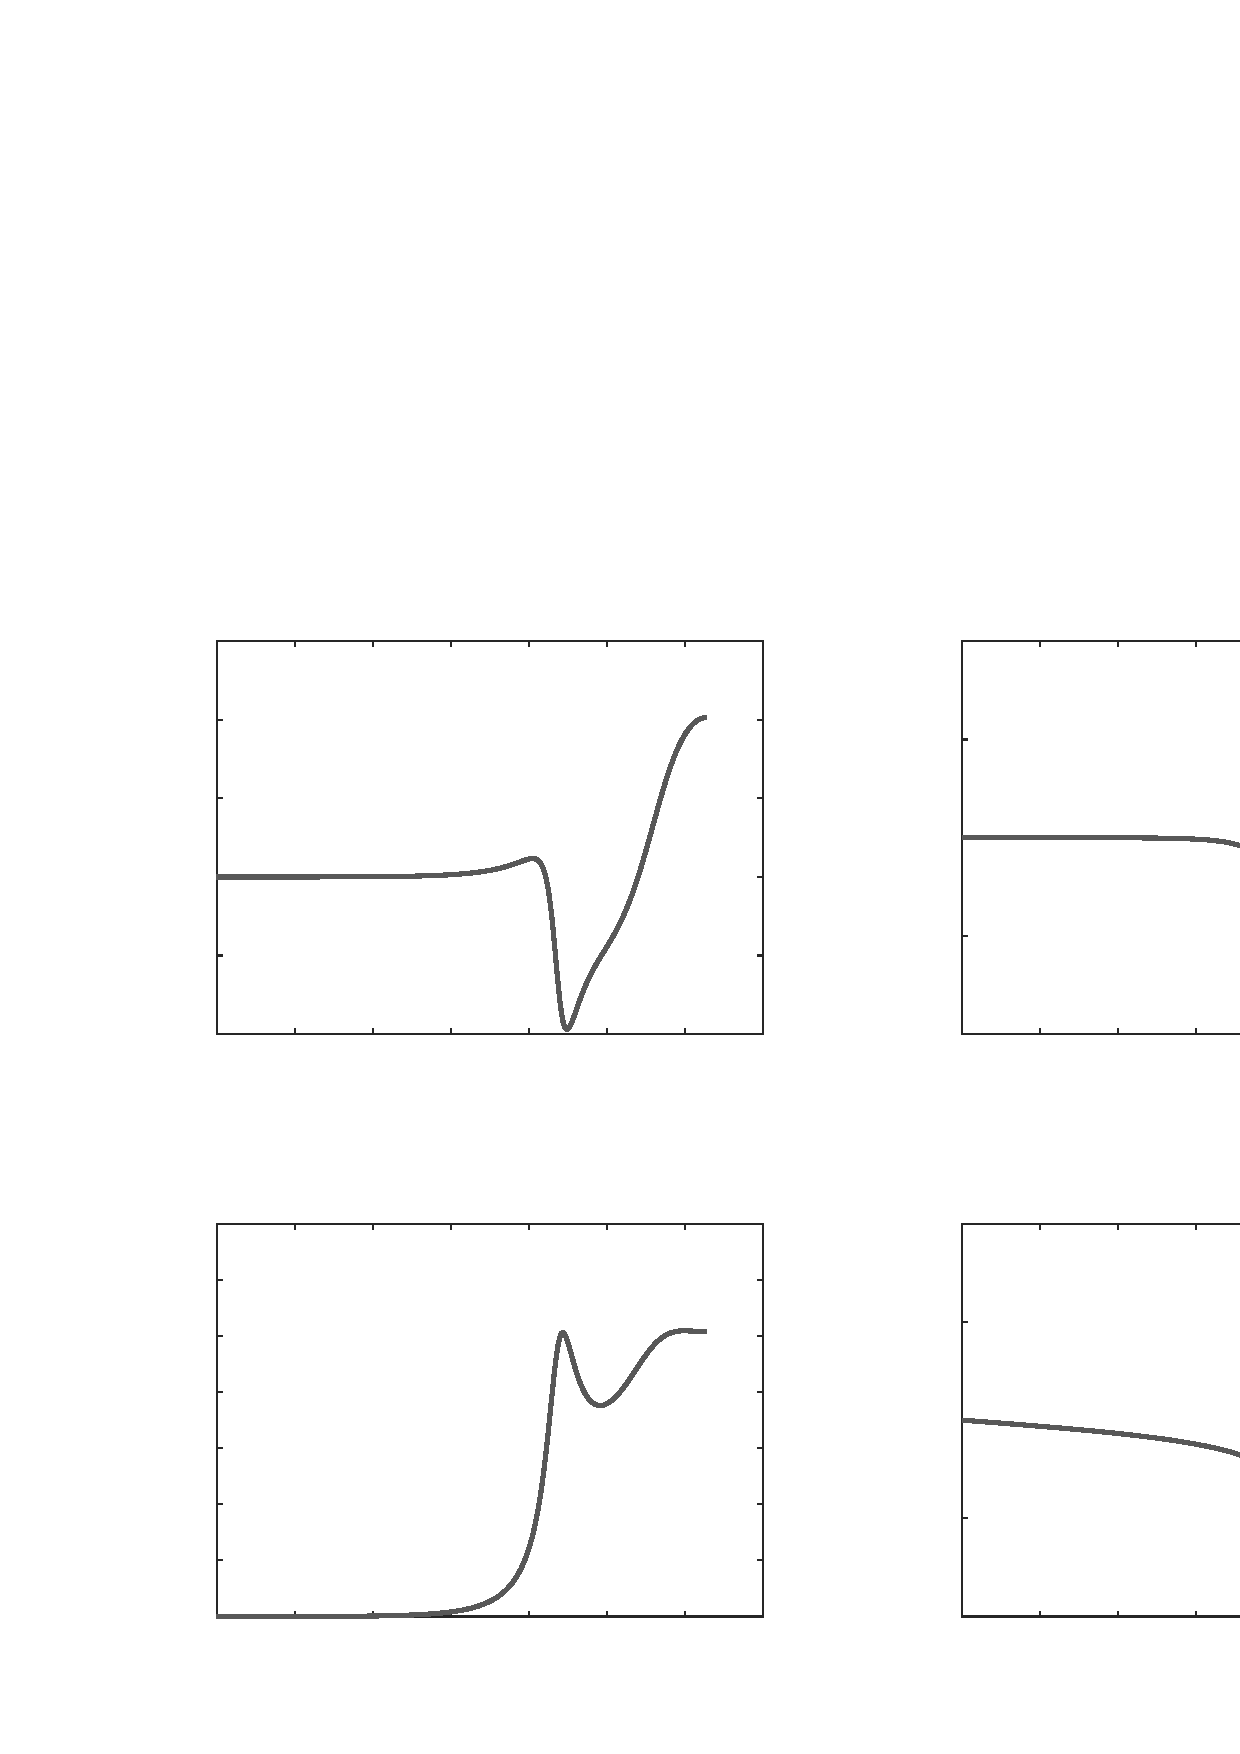
\includegraphics[scale=1]{octaves/dtft-example-inc}
\end{picture}%
\begin{picture}(800,600)(0,0)
\fontsize{13}{0}\selectfont\put(104,335.128){\makebox(0,0)[t]{\textcolor[rgb]{0.15,0.15,0.15}{{0}}}}
\fontsize{13}{0}\selectfont\put(141.438,335.128){\makebox(0,0)[t]{\textcolor[rgb]{0.15,0.15,0.15}{{0.5}}}}
\fontsize{13}{0}\selectfont\put(178.875,335.128){\makebox(0,0)[t]{\textcolor[rgb]{0.15,0.15,0.15}{{1}}}}
\fontsize{13}{0}\selectfont\put(216.313,335.128){\makebox(0,0)[t]{\textcolor[rgb]{0.15,0.15,0.15}{{1.5}}}}
\fontsize{13}{0}\selectfont\put(253.75,335.128){\makebox(0,0)[t]{\textcolor[rgb]{0.15,0.15,0.15}{{2}}}}
\fontsize{13}{0}\selectfont\put(291.188,335.128){\makebox(0,0)[t]{\textcolor[rgb]{0.15,0.15,0.15}{{2.5}}}}
\fontsize{13}{0}\selectfont\put(328.625,335.128){\makebox(0,0)[t]{\textcolor[rgb]{0.15,0.15,0.15}{{3}}}}
\fontsize{13}{0}\selectfont\put(366.063,335.128){\makebox(0,0)[t]{\textcolor[rgb]{0.15,0.15,0.15}{{3.5}}}}
\fontsize{13}{0}\selectfont\put(97.0508,345.577){\makebox(0,0)[r]{\textcolor[rgb]{0.15,0.15,0.15}{{-1}}}}
\fontsize{13}{0}\selectfont\put(97.0508,383.277){\makebox(0,0)[r]{\textcolor[rgb]{0.15,0.15,0.15}{{-0.5}}}}
\fontsize{13}{0}\selectfont\put(97.0508,420.977){\makebox(0,0)[r]{\textcolor[rgb]{0.15,0.15,0.15}{{0}}}}
\fontsize{13}{0}\selectfont\put(97.0508,458.677){\makebox(0,0)[r]{\textcolor[rgb]{0.15,0.15,0.15}{{0.5}}}}
\fontsize{13}{0}\selectfont\put(97.0508,496.377){\makebox(0,0)[r]{\textcolor[rgb]{0.15,0.15,0.15}{{1}}}}
\fontsize{13}{0}\selectfont\put(97.0508,534.077){\makebox(0,0)[r]{\textcolor[rgb]{0.15,0.15,0.15}{{1.5}}}}
\fontsize{15}{0}\selectfont\put(235.032,544.077){\makebox(0,0)[b]{\textcolor[rgb]{0,0,0}{{Real part of H}}}}
\fontsize{13}{0}\selectfont\put(461.937,335.128){\makebox(0,0)[t]{\textcolor[rgb]{0.15,0.15,0.15}{{0}}}}
\fontsize{13}{0}\selectfont\put(499.375,335.128){\makebox(0,0)[t]{\textcolor[rgb]{0.15,0.15,0.15}{{0.5}}}}
\fontsize{13}{0}\selectfont\put(536.812,335.128){\makebox(0,0)[t]{\textcolor[rgb]{0.15,0.15,0.15}{{1}}}}
\fontsize{13}{0}\selectfont\put(574.25,335.128){\makebox(0,0)[t]{\textcolor[rgb]{0.15,0.15,0.15}{{1.5}}}}
\fontsize{13}{0}\selectfont\put(611.687,335.128){\makebox(0,0)[t]{\textcolor[rgb]{0.15,0.15,0.15}{{2}}}}
\fontsize{13}{0}\selectfont\put(649.125,335.128){\makebox(0,0)[t]{\textcolor[rgb]{0.15,0.15,0.15}{{2.5}}}}
\fontsize{13}{0}\selectfont\put(686.562,335.128){\makebox(0,0)[t]{\textcolor[rgb]{0.15,0.15,0.15}{{3}}}}
\fontsize{13}{0}\selectfont\put(724,335.128){\makebox(0,0)[t]{\textcolor[rgb]{0.15,0.15,0.15}{{3.5}}}}
\fontsize{13}{0}\selectfont\put(454.988,345.577){\makebox(0,0)[r]{\textcolor[rgb]{0.15,0.15,0.15}{{-1}}}}
\fontsize{13}{0}\selectfont\put(454.988,392.702){\makebox(0,0)[r]{\textcolor[rgb]{0.15,0.15,0.15}{{-0.5}}}}
\fontsize{13}{0}\selectfont\put(454.988,439.827){\makebox(0,0)[r]{\textcolor[rgb]{0.15,0.15,0.15}{{0}}}}
\fontsize{13}{0}\selectfont\put(454.988,486.952){\makebox(0,0)[r]{\textcolor[rgb]{0.15,0.15,0.15}{{0.5}}}}
\fontsize{13}{0}\selectfont\put(454.988,534.077){\makebox(0,0)[r]{\textcolor[rgb]{0.15,0.15,0.15}{{1}}}}
\fontsize{15}{0}\selectfont\put(592.969,544.077){\makebox(0,0)[b]{\textcolor[rgb]{0,0,0}{{Imaginary part of H}}}}
\fontsize{13}{0}\selectfont\put(104,55.551){\makebox(0,0)[t]{\textcolor[rgb]{0.15,0.15,0.15}{{0}}}}
\fontsize{13}{0}\selectfont\put(141.438,55.551){\makebox(0,0)[t]{\textcolor[rgb]{0.15,0.15,0.15}{{0.5}}}}
\fontsize{13}{0}\selectfont\put(178.875,55.551){\makebox(0,0)[t]{\textcolor[rgb]{0.15,0.15,0.15}{{1}}}}
\fontsize{13}{0}\selectfont\put(216.313,55.551){\makebox(0,0)[t]{\textcolor[rgb]{0.15,0.15,0.15}{{1.5}}}}
\fontsize{13}{0}\selectfont\put(253.75,55.551){\makebox(0,0)[t]{\textcolor[rgb]{0.15,0.15,0.15}{{2}}}}
\fontsize{13}{0}\selectfont\put(291.188,55.551){\makebox(0,0)[t]{\textcolor[rgb]{0.15,0.15,0.15}{{2.5}}}}
\fontsize{13}{0}\selectfont\put(328.625,55.551){\makebox(0,0)[t]{\textcolor[rgb]{0.15,0.15,0.15}{{3}}}}
\fontsize{13}{0}\selectfont\put(366.063,55.551){\makebox(0,0)[t]{\textcolor[rgb]{0.15,0.15,0.15}{{3.5}}}}
\fontsize{13}{0}\selectfont\put(97.0508,66){\makebox(0,0)[r]{\textcolor[rgb]{0.15,0.15,0.15}{{0}}}}
\fontsize{13}{0}\selectfont\put(97.0508,92.9285){\makebox(0,0)[r]{\textcolor[rgb]{0.15,0.15,0.15}{{0.2}}}}
\fontsize{13}{0}\selectfont\put(97.0508,119.857){\makebox(0,0)[r]{\textcolor[rgb]{0.15,0.15,0.15}{{0.4}}}}
\fontsize{13}{0}\selectfont\put(97.0508,146.786){\makebox(0,0)[r]{\textcolor[rgb]{0.15,0.15,0.15}{{0.6}}}}
\fontsize{13}{0}\selectfont\put(97.0508,173.714){\makebox(0,0)[r]{\textcolor[rgb]{0.15,0.15,0.15}{{0.8}}}}
\fontsize{13}{0}\selectfont\put(97.0508,200.643){\makebox(0,0)[r]{\textcolor[rgb]{0.15,0.15,0.15}{{1}}}}
\fontsize{13}{0}\selectfont\put(97.0508,227.571){\makebox(0,0)[r]{\textcolor[rgb]{0.15,0.15,0.15}{{1.2}}}}
\fontsize{13}{0}\selectfont\put(97.0508,254.5){\makebox(0,0)[r]{\textcolor[rgb]{0.15,0.15,0.15}{{1.4}}}}
\fontsize{15}{0}\selectfont\put(235.032,264.5){\makebox(0,0)[b]{\textcolor[rgb]{0,0,0}{{Magnitude spectrum of H}}}}
\fontsize{13}{0}\selectfont\put(461.937,55.6063){\makebox(0,0)[t]{\textcolor[rgb]{0.15,0.15,0.15}{{0}}}}
\fontsize{13}{0}\selectfont\put(499.375,55.6063){\makebox(0,0)[t]{\textcolor[rgb]{0.15,0.15,0.15}{{0.5}}}}
\fontsize{13}{0}\selectfont\put(536.812,55.6063){\makebox(0,0)[t]{\textcolor[rgb]{0.15,0.15,0.15}{{1}}}}
\fontsize{13}{0}\selectfont\put(574.25,55.6063){\makebox(0,0)[t]{\textcolor[rgb]{0.15,0.15,0.15}{{1.5}}}}
\fontsize{13}{0}\selectfont\put(611.687,55.6063){\makebox(0,0)[t]{\textcolor[rgb]{0.15,0.15,0.15}{{2}}}}
\fontsize{13}{0}\selectfont\put(649.125,55.6063){\makebox(0,0)[t]{\textcolor[rgb]{0.15,0.15,0.15}{{2.5}}}}
\fontsize{13}{0}\selectfont\put(686.562,55.6063){\makebox(0,0)[t]{\textcolor[rgb]{0.15,0.15,0.15}{{3}}}}
\fontsize{13}{0}\selectfont\put(724,55.6063){\makebox(0,0)[t]{\textcolor[rgb]{0.15,0.15,0.15}{{3.5}}}}
\fontsize{13}{0}\selectfont\put(454.988,66){\makebox(0,0)[r]{\textcolor[rgb]{0.15,0.15,0.15}{{-4}}}}
\fontsize{13}{0}\selectfont\put(454.988,113.125){\makebox(0,0)[r]{\textcolor[rgb]{0.15,0.15,0.15}{{-2}}}}
\fontsize{13}{0}\selectfont\put(454.988,160.25){\makebox(0,0)[r]{\textcolor[rgb]{0.15,0.15,0.15}{{0}}}}
\fontsize{13}{0}\selectfont\put(454.988,207.375){\makebox(0,0)[r]{\textcolor[rgb]{0.15,0.15,0.15}{{2}}}}
\fontsize{13}{0}\selectfont\put(454.988,254.5){\makebox(0,0)[r]{\textcolor[rgb]{0.15,0.15,0.15}{{4}}}}
\fontsize{15}{0}\selectfont\put(592.969,264.5){\makebox(0,0)[b]{\textcolor[rgb]{0,0,0}{{Phase spectrum of H}}}}
\end{picture}

}\caption{\emph{Real part}, \emph{imaginary part}, \emph{magnitude spectrum} and \emph{phase spectrum} plots of Example~\ref{eqn:octaveExampleFreqz}. Notice the discontinuity in the $\arctan{}$ function that manifests with a sudden jump in the phase spectrum. Plots have been generated with the help of \texttt{octave}.}\label{oct:octaveExampleFreqz}
    \end{center}
\end{figure}
\clearpage

\subsection{The Unwrapped Phase Function}
In numerical computation when the computed phase function is outside of the possible range of $\omega$---that is $[-\pi, \pi]$---to bring the computed value to the correct range the phase is computed \emph{modulo} $2\pi$. Hence, the phase may exhibit some discontinuities of $2\pi$ radians in the phase spectrum plot, as in Figure~\ref{oct:octaveExampleFreqz}. Indeed, one would like to possess some kind of representation which doesn't present any kind of visible discontinuity; to do so, one should adopt the \textbf{unwrapped phase function}.

Unwrapped phase functions are special functions whose goal is to represent the phase without any dis\-con\-ti\-nui\-ty---that is, by \emph{unwrapping the phase}. Related function goes under the name of $\theta_c(\omega)$. In the following Figure~\ref{oct:octaveExampleFreqzUnwrap} the unwrapped phase spectrum has been plotted with the commands
\begin{verbatim}
plot(w,unwrap(angle(H)));
\end{verbatim}
which are enough to produce a plot of the desired unwrapped phase function of \texttt{H}.

% print -depslatex -mono "-S800,600" "figure-name.tex"
\begin{figure}[ht]
    \begin{center}
\scalebox{0.6}{
% Title: gl2ps_renderer figure
% Creator: GL2PS 1.4.2, (C) 1999-2020 C. Geuzaine
% For: Octave
% CreationDate: Wed Oct 19 08:41:45 2022
\setlength{\unitlength}{1pt}
\begin{picture}(0,0)
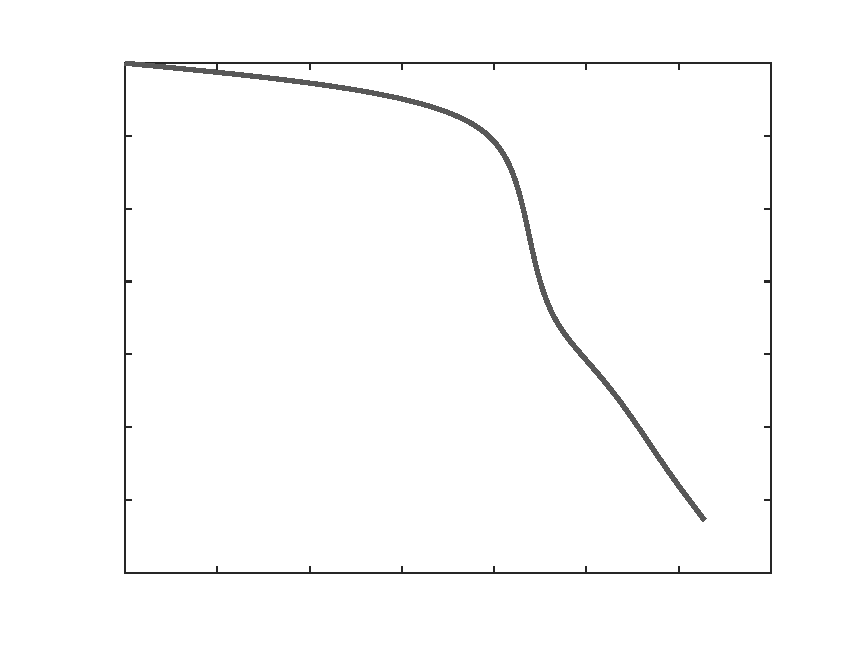
\includegraphics[scale=1]{octaves/dtft-unwrap-inc}
\end{picture}%
\begin{picture}(400,300)(0,0)
\fontsize{6}{0}\selectfont\put(52,27.7787){\makebox(0,0)[t]{\textcolor[rgb]{0.15,0.15,0.15}{{0}}}}
\fontsize{6}{0}\selectfont\put(96.2857,27.7787){\makebox(0,0)[t]{\textcolor[rgb]{0.15,0.15,0.15}{{0.5}}}}
\fontsize{6}{0}\selectfont\put(140.571,27.7787){\makebox(0,0)[t]{\textcolor[rgb]{0.15,0.15,0.15}{{1}}}}
\fontsize{6}{0}\selectfont\put(184.857,27.7787){\makebox(0,0)[t]{\textcolor[rgb]{0.15,0.15,0.15}{{1.5}}}}
\fontsize{6}{0}\selectfont\put(229.143,27.7787){\makebox(0,0)[t]{\textcolor[rgb]{0.15,0.15,0.15}{{2}}}}
\fontsize{6}{0}\selectfont\put(273.429,27.7787){\makebox(0,0)[t]{\textcolor[rgb]{0.15,0.15,0.15}{{2.5}}}}
\fontsize{6}{0}\selectfont\put(317.714,27.7787){\makebox(0,0)[t]{\textcolor[rgb]{0.15,0.15,0.15}{{3}}}}
\fontsize{6}{0}\selectfont\put(362,27.7787){\makebox(0,0)[t]{\textcolor[rgb]{0.15,0.15,0.15}{{3.5}}}}
\fontsize{6}{0}\selectfont\put(48.5263,33){\makebox(0,0)[r]{\textcolor[rgb]{0.15,0.15,0.15}{{-7}}}}
\fontsize{6}{0}\selectfont\put(48.5263,67.9286){\makebox(0,0)[r]{\textcolor[rgb]{0.15,0.15,0.15}{{-6}}}}
\fontsize{6}{0}\selectfont\put(48.5263,102.857){\makebox(0,0)[r]{\textcolor[rgb]{0.15,0.15,0.15}{{-5}}}}
\fontsize{6}{0}\selectfont\put(48.5263,137.786){\makebox(0,0)[r]{\textcolor[rgb]{0.15,0.15,0.15}{{-4}}}}
\fontsize{6}{0}\selectfont\put(48.5263,172.714){\makebox(0,0)[r]{\textcolor[rgb]{0.15,0.15,0.15}{{-3}}}}
\fontsize{6}{0}\selectfont\put(48.5263,207.643){\makebox(0,0)[r]{\textcolor[rgb]{0.15,0.15,0.15}{{-2}}}}
\fontsize{6}{0}\selectfont\put(48.5263,242.571){\makebox(0,0)[r]{\textcolor[rgb]{0.15,0.15,0.15}{{-1}}}}
\fontsize{6}{0}\selectfont\put(48.5263,277.5){\makebox(0,0)[r]{\textcolor[rgb]{0.15,0.15,0.15}{{0}}}}
\end{picture}

}\caption{\emph{Unwrapped} phase spectrum plot of phase spectrum of Example~\ref{eqn:octaveExampleFreqz}. By employing \texttt{unwrap} function in \texttt{octave}, the discontinuity in the $\arctan{}$ function had disappeared.}\label{oct:octaveExampleFreqzUnwrap}
    \end{center}
\end{figure}
Undeniably, the unwrapped representation remains imperative when plotting phase spectra.

\subsection{The Convolution Theorem}\label{sec:convolutionTheorem}

The discrete-time Fourier transform (DTFT) is a form of Fourier analysis that is applicable to a sequence of values.

The DTFT is often used to analyze samples of a continuous function. The term discrete-time refers to the fact that the transform operates on discrete data, often samples whose interval has units of time. From uniformly spaced samples it produces a function of frequency that is a periodic summation of the continuous Fourier transform of the original continuous function. Under certain theoretical conditions, described by the sampling theorem, the original continuous function can be recovered perfectly from the DTFT and thus from the original discrete samples. The DTFT itself is a continuous function of frequency, but discrete samples of it can be readily calculated via the discrete Fourier transform (DFT), which is by far the most common method of modern Fourier analysis.

Indeed, a paramount property that surely helps when it comes to performing convolutions on the time-domain is the following, remarkable property, that goes under the name of \textbf{Convolution Theorem}.
\begin{thm}[Convolution Theorem]
    Consider two signals $g(x)$ and $h(x)$ whose Fourier Transforms are $G(\omega)$ and $H(\omega)$, and let $\mathcal F\{\cdot\}$ denote the operator of Fourier Transformation. The convolution of $g$ and $h$ is defined by
    \begin{equation}\label{eqn:convolutionTheorem}
        g \circledast h = \mathcal F^{-1}\{G \cdot H\},
    \end{equation}
    where a convolution sum in the time-domain corresponds to a \emph{product} in the frequency domain.
\end{thm}

The Convolution Theorem states that any convolution sum can be performed as a product in the frequency domain. This also means that no matter the signals' domain, jumping into the related frequency domain and performing a product of the Fourier Transforms of the two signals is a straightforward way to perform a convolution sum.
An immediate application of this crucial result is that the linear convolution $y[n]$ of $x[n]$ and $h[n]$ in a linear discrete-time system can be performed \emph{much} more quickly by going for the frequency-domain route. The steps of this faster process are the following ones,
\begin{enumerate}
    \item first, one computes the discrete-time Fourier Transforms of $x$ and $h$, that are $X(e^{j\omega})$ and $H(e^{j\omega})$;
    \item second, from the frequency-domain one quickly evaluates $Y(e^{j\omega}) = X(e^{j\omega})\cdot H(e^{j\omega})$;
    \item and at last, to obtain $y[n]$ it is enough to compute the inverse DTFT. The overall process is depicted in Figure~\ref{tikz:linearConvolutionFrequencyDomain}.
\end{enumerate}
\begin{figure}[ht]
\begin{center}
    \begin{tikzpicture}
    \node [](Xi){$x[n]$};
    \node [](Hi) at (0, -2){$h[n]$};
    \node [draw, boxfilter](DTFTX) at (2, 0) {DTFT};
    \node [draw, boxfilter](DTFTH) at (2, -2) {DTFT};
    \node [label=north:{$X(e^{j\omega})$}](X) at (3.3, 0){};
    \node [label=north:{$H(e^{j\omega})$}](H) at (3.3, -2){};
    \node [draw, circle, crossp, thick, minimum size=.5cm](PROD) at (4, -1) {};
    \node [draw, boxfilter](IDTFTY) at (6, -1) {DTFT};
    \node [](Yo) at (7.5, -1){$y[n]$};

    \draw[-stealth] (Xi) -- (DTFTX);
    \draw[-stealth] (Hi) -- (DTFTH);
    \draw[-stealth] (DTFTX) -| (PROD);
    \draw[-stealth] (DTFTH) -| (PROD);
    \draw[-stealth] (PROD) -- (IDTFTY);
    \draw[-stealth] (IDTFTY) -- (Yo);
\end{tikzpicture}\caption{Linear convolution as a product in frequency domain. In reality, the process is not performed, as it is far from convenient to handle continuous signals.}\label{tikz:linearConvolutionFrequencyDomain}
\end{center}
\end{figure}

The aforementioned procedure is not feasible in reality for two reasons: first of all, it is never convenient---let alone possible---to effectively handle \emph{continuous} signals. Indeed, no machine can possibly compute all the infinite points required for the computation. Secondarily and not less importantly, the inverse discrete-time Fourier Transform is an \emph{integral}. Performing integrations on a continuous is far from efficient for the same reasons as above.

With the Convolution Theorem ends the chapter on Discrete-time Fourier Transforms. Indeed, as we will see, the Convolution Theorem will prove useful even for the next subject of study, the \emph{Discrete Fourier Transforms}.


\chapter{Discrete Fourier Transform}

In mathematics, the discrete Fourier transform (DFT) converts a finite sequence of equally-spaced samples of a function into a same-length sequence of equally-spaced samples of the discrete-time Fourier transform (DTFT), which is a complex-valued function of frequency. The interval at which the DTFT is sampled is the reciprocal of the duration of the input sequence. An inverse DFT is a Fourier series, using the DTFT samples as coefficients of complex sinusoids at the corresponding DTFT frequencies. It has the same sample-values as the original input sequence. The DFT is therefore said to be a frequency domain representation of the original input sequence. If the original sequence spans all the non-zero values of a function, its DTFT is continuous (and periodic), and the DFT provides discrete samples of one cycle. If the original sequence is one cycle of a periodic function, the DFT provides all the non-zero values of one DTFT cycle.

The DFT is the most important discrete transform, used to perform Fourier analysis in many practical applications. In digital signal processing, the function is any quantity or signal that varies over time, such as the pressure of a sound wave, a radio signal, or daily temperature readings, sampled over a finite time interval (often defined by a window function). In image processing, the samples can be the values of pixels along a row or column of a raster image. The DFT is also used to efficiently solve partial differential equations, and to perform other operations such as convolutions or multiplying large integers.

Since it deals with a \textbf{finite} amount of data, it can be implemented in computers by numerical algorithms or even dedicated hardware. These implementations usually employ efficient fast Fourier transform (FFT) algorithms; so much so that the terms ``FFT'' and ``DFT'' are often used interchangeably. Prior to its current usage, the ``FFT'' initialism may have also been used for the ambiguous term ``finite Fourier transform''~\cite{bib:discreteFourierTransform}.

\section{Orthogonal Transforms}\label{sec:orthogonalTransforms}

Let $x[n]$ be a sequence of length $N$. We define $\mathcal X[k], 0 \leq k \leq N-1$ the $N$-point \textbf{orthogonal transform} of $x[n]$. An orthogonal transforms is a \emph{generalized} version of Transforms that takes the form
\begin{eqnarray}
    \mathcal X[k] = \sum_{n=0}^{N-1} x[n] \psi^*[k,n], & 0 \leq k \leq N-1, \\\label{eqn:analysisEquationDTFT}
    x[k] = \sum_{k=0}^{N-1} \mathcal X[n] \psi[k,n], & 0 \leq n \leq N-1. \label{eqn:synthesisEquationDTFT}
\end{eqnarray}
The first Equation~\ref{eqn:analysisEquationDTFT} is called \emph{Analysis equation}, while the second Equation~\ref{eqn:synthesisEquationDTFT} is said to be the \emph{Synthesis equation}. Both analysis and synthesis equations concur in the definition of the orthogonal transform. Indeed, the analysis equation allows to perform the orthogonal transformation, while implicitly the synthesis equation serves as a ``inverse'' orthogonal transform. Still, the $\psi$ are said to be \emph{basis sequences} and are of length $N$ as well as the original sequence and the orthogonal transform sequence. Basis sequences can have complex values, so generally $\psi[k, n] \in \C$. In the class of transforms to be considered in this notes of digital signal processing, all the basis sequences will satisfy the following condition,
\begin{equation}\label{eqn:orthogonalTransformsOrthogonalityCondition}
    \frac 1 N \sum_{n=0}^{N-1} \psi[k,n]\psi^*[l,n] = \left\{\begin{array}{ll}1, & l = k\\ 0, & l \neq k\end{array}\right.,
\end{equation}
a condition that substantially poses that the product \[\psi[k,n]\psi^*[l,n]\] is equal to $1$ if and only if indexes $l = k$, a property that if satisfied then the basis sequences are said to be \emph{orthogonal to each other}.

Really, in order for $\psi^*$ to be the inverse orthogonal transform, $\psi$ and $\psi^*$ have to be orthogonal to each other. This can be verified by substituting the synthesis equation~\ref{eqn:synthesisEquationDTFT} into the analysis equation~\ref{eqn:analysisEquationDTFT},
\begin{align*}
    \sum_{n=0}^{N-1} x[n] \psi^*[k,n] &= \sum_{n=0}^{N-1}\left( \frac 1 N \sum_{k=0}^{N-1} \mathcal X[k] \psi[n,k]\right)\psi^*[l,n] \\
                                      &= \sum_{k=0}^{N-1} \mathcal X[k] \left( \frac 1 N \sum_{n=0}^{N-1}\psi[n,k]\psi^*[l,n]\right) \\
                                      &= \mathcal X[l],
\end{align*}
which yields an identity. Of course, the other way around works exactly the same, hence the inverse orthogonal transform is expressed as in Equation~\ref{eqn:synthesisEquationDTFT}.

An important consequence of the orthogonality condition for orthogonal transforms is the \textbf{Energy Preservation Property}, which states that
\begin{equation}\label{eqn:energyPreservationProperty}
    \sum_{n=0}^{N-1}|x[n]|^2 = \frac 1 N \sum_{k=0}^{N-1}\left|\mathcal X[n]\right|^2
\end{equation}
Yet, the Energy Preservation Property is more commonly known as the \emph{Parseval's Theorem}, of which it is a more general formulation.

\section{Definition of Discrete Fourier Transform}

It's now the time to introduce the \textbf{Discrete Fourier Transform (DFT)}, a tool of a paramount importance in the field of digital signal processing.

\begin{defin}[Discrete Fourier Transform]
    Let $x[n]$ be a finite-length sequence of length $N$ defined for $0 \leq n \leq N-1$ and be $X(e^{j\omega})$ its discrete-time Fourier Transform as in Equation~\ref{eqn:discreteTimeFourierTransform}. By \emph{uniformly sampling} $X(e^{j\omega})$ on the $\omega$ axis in the interval $[0, 2\pi[$ at samples $\omega_k=\frac{2k\pi}{N}$ for $0 \leq k \leq N-1$ one obtains a sequence $X[k]$ such that
    \begin{equation}\label{eqn:discreteFourierTransform}
        X[k] = X(e^{j\omega})\Bigr\rvert_{\omega = \frac {2k\pi}{N}} = \sum_{n=0}^{N-1} x[n] e^{-2j\pi \frac{k n}{N}}, 0 \leq k \leq N-1
    \end{equation}
    where $X[k]$ is a sequence of length $N$ in the frequency domain represented by the variable $k$. The sequence $X[k]$ is called the \emph{Discrete Fourier Transform (DFT)} of the sequence.
\end{defin}

The above definition has been obtained by sampling the $\omega$ frequency variable in samples $2k\pi / N$ so that the complex continuous exponential $e^{-j\omega}$ has become $e^{-2j\pi \frac{kn}{N}}$. Usually, in order to streamline the notation, the substitution
\begin{equation}\label{eqn:dftNotationWn}
    W_N = e^{-j\frac{2\pi}{N}}
\end{equation}
under which the Discrete Fourier Transform now is rewritten into the following,
\begin{equation}\label{eqn:discreteTimeFourierTransformWn}
        X[k] = \sum_{n=0}^{N-1} x[n] W_N^{kn}, 0 \leq k \leq N-1.
\end{equation}

The notation expressed in~\ref{eqn:dftNotationWn} renders the orthogonal transform operator $W_N$ in Discrete Fourier Transform sum have a positive sign in its exponents. This behavior is the opposite of what one encounters by looking at the original definition.

Along with the DFT, the \textbf{Inverse Discrete Fourier Transform} should be defined as well in order to produce meaningful computations. Indeed,
\begin{equation}\label{eqn:inverseDiscreteFourierTransformWn}
    x[k] = \sum_{k=0}^{N-1} X[k] W_N^{-kn}, 0 \leq n \leq N-1,
\end{equation}
expressed under the new notation\footnote{
    The original Discrete Fourier Transform---without employing the new notation---would be
    \[
        x[k] = \sum_{k=0}^{N-1} X[k] e^{2j\pi\frac{kn}{N}}, 0 \leq n \leq N-1,
    \]
    showing a positive sign at the exponentiation.
}. The inverse Discrete Fourier Transform is \emph{periodic} as well.
Verifying the above inverse transform is straightforward, as it is enough to substitute the original transform into the inverse, then multiply both sides of the equation by $W_N^{ln}$ and sum the result from $n=0$ to $n=N-1$. Of course,
\begin{align*}
    \sum_{n=0}^{N-1} x[n] W_N^{ln}
    &= \sum_{n=0}^{N-1}\left(\frac 1 N\sum_{k=0}^{K-1} X[k] W_N^{-kn}\right)W_n^{ln}\\
    &= \frac 1 N \sum_{n=0}^{N-1}\sum_{k=0}^{K-1} X[k] W_N^{-(k-l)n}\\
    &= \frac 1 N \sum_{k=0}^{K-1} X[k] \left(\sum_{n=0}^{N-1}W_N^{-(k-l)n}\right).
\end{align*}
Now, since
\begin{equation}\label{eqn:dftWnProperty}
    \sum_{n=0}^{N-1}W_N^{-(k-l)n} = \left\{\begin{array}{ll} N, & k - l = rN, r \in \Z\\ 0, & \mbox{otherwise}\end{array}\right.
\end{equation}
due to the exponentiation properties. In order to verify that, just substitute with the definition of $W_N$, that is \[\sum_{n=0}^{N-1}e^{+2j\pi\frac{(k-l)n}{N}},\] a quantity that indeed is equal to $N$ if and only if $k-l$ is a multiple of $N$ and $0$ otherwise. The term relative to $n=0$ is the sum of $N$ terms all equal to $1$, while the term for $n\neq 0$ is related to the first $N$ terms of a geometric progression, that are \[\sum_{n=0}^{N-1}\rho^n = \frac{1-\rho^N}{1 - \rho} = 0\] as the exponential $e^{j2\pi\frac{N}{N}} = 1$. Another way to see it is to consider that a set of $W_N$ vectors is summed together---when $k\neq l$ for each vector of phase $\varphi$ another vector of opposite phase $-\varphi$ is summed, and the result of the sum is exactly $0$; on contrary, the only way to avoid the cancellation of terms is when $k = l$, that is when all terms have magnitude equal to $|e^{j2\pi\frac{N}{N}}| = 1$ and possess phase $\varphi = 0$. For this reason, one obtains that the only non-zero term in the sum is $\sum_{n=0}^{N-1} W_N^{-(k-l)n}, k=l, 0\leq l,k \leq N-1$. Hence,
\begin{align*}
    \sum_{n=0}^{N-1} x[n] W_N^{ln}
    &= \frac 1 N \sum_{k=0}^{K-1} X[k] \left(\sum_{n=0}^{N-1}W_N^{-(k-l)n}\right).\\
    &= \frac 1 N X[l] N = X[l].
\end{align*}

\subsection{Basis functions}\label{sec:basisFunctions}

In the end, the Discrete Fourier Transform involves choosing two \textbf{basis functions} $\psi^*$ and $\psi$ with which to carry out the transformation: one \emph{direct},
\[
    \psi^*(n, k) = e^{-j 2\pi \frac{nk}{N}},
\]
and the other \emph{inverse},
\[
    \psi(n, k) = e^{+j 2\pi \frac{nk}{N}},
\]
which are basically the two terms appearing in the sum required to transform a sequence. The notion of two basis functions to produce a transform will become useful later, when other kinds of transformations will be examined. In point of fact, the two basis functions will vary in relation to the specific transform to adopt. As we have seen in Section~\ref{sec:orthogonalTransforms}, \emph{any orthogonal transform can be expressed with their analysis and synthesis equations}, that is
\begin{equation}\label{eqn:analysisEquation}
    X(k) = \sum_{n=0}^{N-1} x(n)\psi^*(n, k),
\end{equation}
known as the \textbf{synthesis equation}; the above leads to the matrix form
\begin{equation}\label{eqn:analysisEquationMatrixForm}
    \bm{X} = \bm{Fx}.
\end{equation}

The matrix $\bm{F}$ must be \emph{unitary}, which means it must satisfy
\begin{equation}\label{eqn:unitaryMatrix}
    \bm{F}^{-1} = \bm{F}^{*\top}.
\end{equation}

Any orthogonal transform also possesses a \textbf{synthesis equation}, which stands for theinverse operation, that can be expressed as
\begin{equation}\label{eqn:synthesisEquation}
    x(n) = \sum_{k=0}^{N-1} X(k)\psi(n, k),
\end{equation}
that leads to
\begin{equation}\label{eqn:synthesisEquationMatrixForm}
    \bm{x} = \bm{F}^{*\top}\bm{x}.
\end{equation}

The presence of the conjugation in the analysis equation is not casual: $\psi$ and $\psi^*$ are, in reality, conjugated versions of each other.

For Parseval's theorem~(\ref{eqn:parsevalTheorem}), when computing $\bm X$ $\bm x$ preserves its length, and the energy is preserved as well,
\[
    \|\bm X\|^2 = \bm X^{*\top} \bm X = \bm x^{*\top}\bm F^{*\top} \bm {Fx} = \bm x^{*\top} \bm x = \|\bm x\|^2.
\]

Matrix $\bm X$ is a rotated version of $\bm x$ in an $N$-dimensional space, as the transform is a rotation of the co\"ordinates where the terms in $\bm X$ are \emph{the projections of $\bm x$ in the new space}. A suitable choice of the basis functions permits to exploit the \emph{energy compaction property} of an orthogonal transform: most of the contents of $\bm x$ can be represented by \emph{a subset} of the coefficients $\bm X$ instead of all of them, leading to much more efficient algorithms and representations.

For instance, let $\bm x$ be a random signal possessing autocorrelation $\bm{R_x}$---the most efficient transform for random signals is the \textbf{Karhunen--Loève Transform (KLT)}, also called \textbf{Hotelling Transform}. The KLT is a transform that takes as basis functions the eigenvectors of the autocorrelation matrix $\bm {R_x}$. 

It is now clear that the DFT is not the only possible tranform, and depending on the scenario other orthogonal transforms can (and should) be used. Sections~\ref{sec:discreteCosineTransform}, \ref{sec:walshHadamardTransform}~and~\ref{sec:haarTransform} will cover some other instrumental orthogonal transforms one can employ in digital signal processing.

\subsection{Example of DTFs}

The first example in exam is a DFT of the following sequence of length $N$,
\[
    x[n] = \left\{\begin{array}{ll}
            1 & n=0\\
            0 & 1 \leq n \leq N-1
        \end{array}\right.
\]
that is quite similar to the delta impulse. Its $N$-point Discrete Fourier Transform is given by
\[
    X[k] = \sum_{n=0}^{N-1} x[n]W_N^{kn} = x[0]W_N^{k0} = 1, 1\leq k \leq N-1.
\]

The second example is of a sequence
\[
    y[n] = \left\{\begin{array}{ll}
            1 & n=m\\
            0 & 0\leq n \leq m-1, m+1 \leq n \leq N-1
        \end{array}\right.
\]
which is like the previous example, but translated of $m$. Its Discrete Fourier Transform will be
\[
    Y[k] = \sum_{n=0}^{N-1} y[n]W_N^{kn} = y[m]W_N^{km} = W_N^{km}, 1\leq k \leq N-1.
\]

Let now $g[n] = \cos{2\pi \frac{rn}{N}}$ be a sequence of length $N$. Since
\begin{align*}
    g[n] &= \frac 1 2 \left(e^{j2\pi \frac{rn}{N}} + e^{-j2\pi \frac{rn}{N}}\right)\\
         &= \frac 1 2 \left(W_N^{rn} + W_N^{rn}\right),
\end{align*}
and due to linearity the Discrete Fourier Transform will be the transform of the two addends. Therefore,
\begin{align*}
    G[k] &= \sum_{n=0}^{N-1} g[n] W_N^{kn} \\
         &= \frac 1 2 \left(\sum_{n=0}^{N-1} W_N^{-(r-k)n} + \sum_{n=0}^{N-1} W_N^{-(r+k)n}\right)
\end{align*}
and by means of Identity~\ref{eqn:dftWnProperty} one finally obtains that
\[
    G[k] = \left\{\begin{array}{ll}
            \frac N 2 & k = r\\
            \frac N 2 & k = N - r\\
            0         & \mbox{ otherwise }
    \end{array}\right.
\]

The DFT of a cosine wave is a pair of impulses of amplitude $\frac N 2$, located at samples $r$ and $N-r$ that represent \emph{the same} frequency. Conceptually then, a cosine DFT is a pair of impulses just like in the case of the Discrete-time Fourier Transform.

\subsection{Matrix relations}

Discrete Fourier Transform as expressed in~\ref{eqn:discreteTimeFourierTransformWn} can be easily expressed into a matrix form. Let $\bm x$ and $\bm X$ be two column vectors as defined,
\[
    \bm{x} = \begin{bmatrix} x[0] \\ x[1] \\ \vdots \\ x[N-1] \end{bmatrix}
    \bm{X} = \begin{bmatrix} X[0] \\ X[1] \\ \vdots \\ X[N-1] \end{bmatrix}
\]
the \emph{Matrix form of the Discrete Fourier Transform} is
\begin{equation}\label{eqn:dftMatrixForm}
    \bm{X} = \bm{D}_N\bm{x}
\end{equation}
with $\bm D_N$ the \textbf{DFT Matrix}, a $N \times N$ matrix given by
\begin{equation}\label{eqn:dftMatrixDn}
    \bm D_N = \begin{bmatrix}
        1 & 1 & 1 & \cdots & 1 \\
        1 & W_N^1 & W_N^2 & \cdots & W_N^{(N-1)} \\
        1 & W_N^2 & W_N^4 & \cdots & W_N^{2(N-1)} \\
        \vdots & \vdots & \vdots & \ddots & \vdots \\
        1 & W_N^{(N-1)} & W_N^{2(N-1)} & \cdots & W_N^{(N-1)^2} \\
    \end{bmatrix}
\end{equation}

Conversely, the \emph{Matrix form of the Inverse Discrete Fourier Transform} is given by a similar relationship,
\begin{equation}\label{eqn:idftMatrixForm}
    \bm{x} = \bm{D}^{-1}_N\bm{X}
\end{equation}
with $\bm D_N$ the \textbf{Inverse DFT Matrix}, a $N \times N$ matrix given by
\begin{equation}\label{eqn:idftMatrixDn}
    \bm D^{-1}_N = \frac 1 N\begin{bmatrix}
        1 & 1 & 1 & \cdots & 1 \\
        1 & W_N^{-1} & W_N^{-2} & \cdots & W_N^{-(N-1)} \\
        1 & W_N^{-2} & W_N^{-4} & \cdots & W_N^{-2(N-1)} \\
        \vdots & \vdots & \vdots & \ddots & \vdots \\
        1 & W_N^{-(N-1)} & W_N^{-2(N-1)} & \cdots & W_N^{-(N-1)^2} \\
    \end{bmatrix}
\end{equation}

Remarkably, the following relationship holds between the inverse and the straight DFT Matrix,
\[
    \bm D_N = \frac 1 N \bm D^{-1}_N,
\]
with a factor of $\frac 1 N$ between the one and the other.

Matrix relations are crucial to learn how to manipulate Discrete Fourier Transforms in \textsc{Matlab}. In fact, the two functions \texttt{fft} and \texttt{ifft}---which stand for \emph{Fast Fourier Transform} and \emph{Inverse Fast Fourier Transform}---manipulate column vector data structures. These two functions make use of sophisticated techniques and efficient algorithms based on the ``dividi et impera'' concept to optimize the computation of the DFT.

Let's study the DFT of the cosine $\cos{2\pi r \frac{n}{N}}$. The following \texttt{octave} code computes and plots the DFT of such function, first by setting $r=3$, then with $r=3.3$.
\begin{verbatim}
N = 21;
M = 21;
r = 3; n = 0:N-1;  u = cos(2*pi*r*n/N);
U = fft(u,M);
figure(1);
subplot(2,3,1);   n = 0:1:N-1;   stem(n,u);
title('Original time-domain sequence');
xlabel('Time index n'); ylabel('Amplitude')
subplot(2,3,2);   k = 0:1:M-1;   stem(k,abs(U));
title('Magnitude, r = 3');
xlabel('Frequency index k'); ylabel('Magnitude')
subplot(2,3,3);   stem(k,angle(U));
title('Phase, r = 3');
xlabel('Frequency index k'); ylabel('Phase')
\end{verbatim}

\begin{verbatim}
r = 3.3; n = 0:N-1;  u = cos(2*pi*r*n/N);
U = fft(u,M);
subplot(2,3,4);   n = 0:1:N-1;   stem(n,u);
title('Original time-domain sequence');
xlabel('Time index n'); ylabel('Amplitude')
subplot(2,3,5);   k = 0:1:M-1;   stem(k,abs(U));
title('Magnitude, r = 3.3');
xlabel('Frequency index k'); ylabel('Magnitude')
subplot(2,3,6);   stem(k,angle(U));
title('Phase, r = 3.3');
xlabel('Frequency index k'); ylabel('Phase')
\end{verbatim}

\begin{figure*}[ht]
\begin{center}
\scalebox{0.6}{
% Title: gl2ps_renderer figure
% Creator: GL2PS 1.4.2, (C) 1999-2020 C. Geuzaine
% For: Octave
% CreationDate: Wed Oct 19 16:31:04 2022
\setlength{\unitlength}{1pt}
\begin{picture}(0,0)
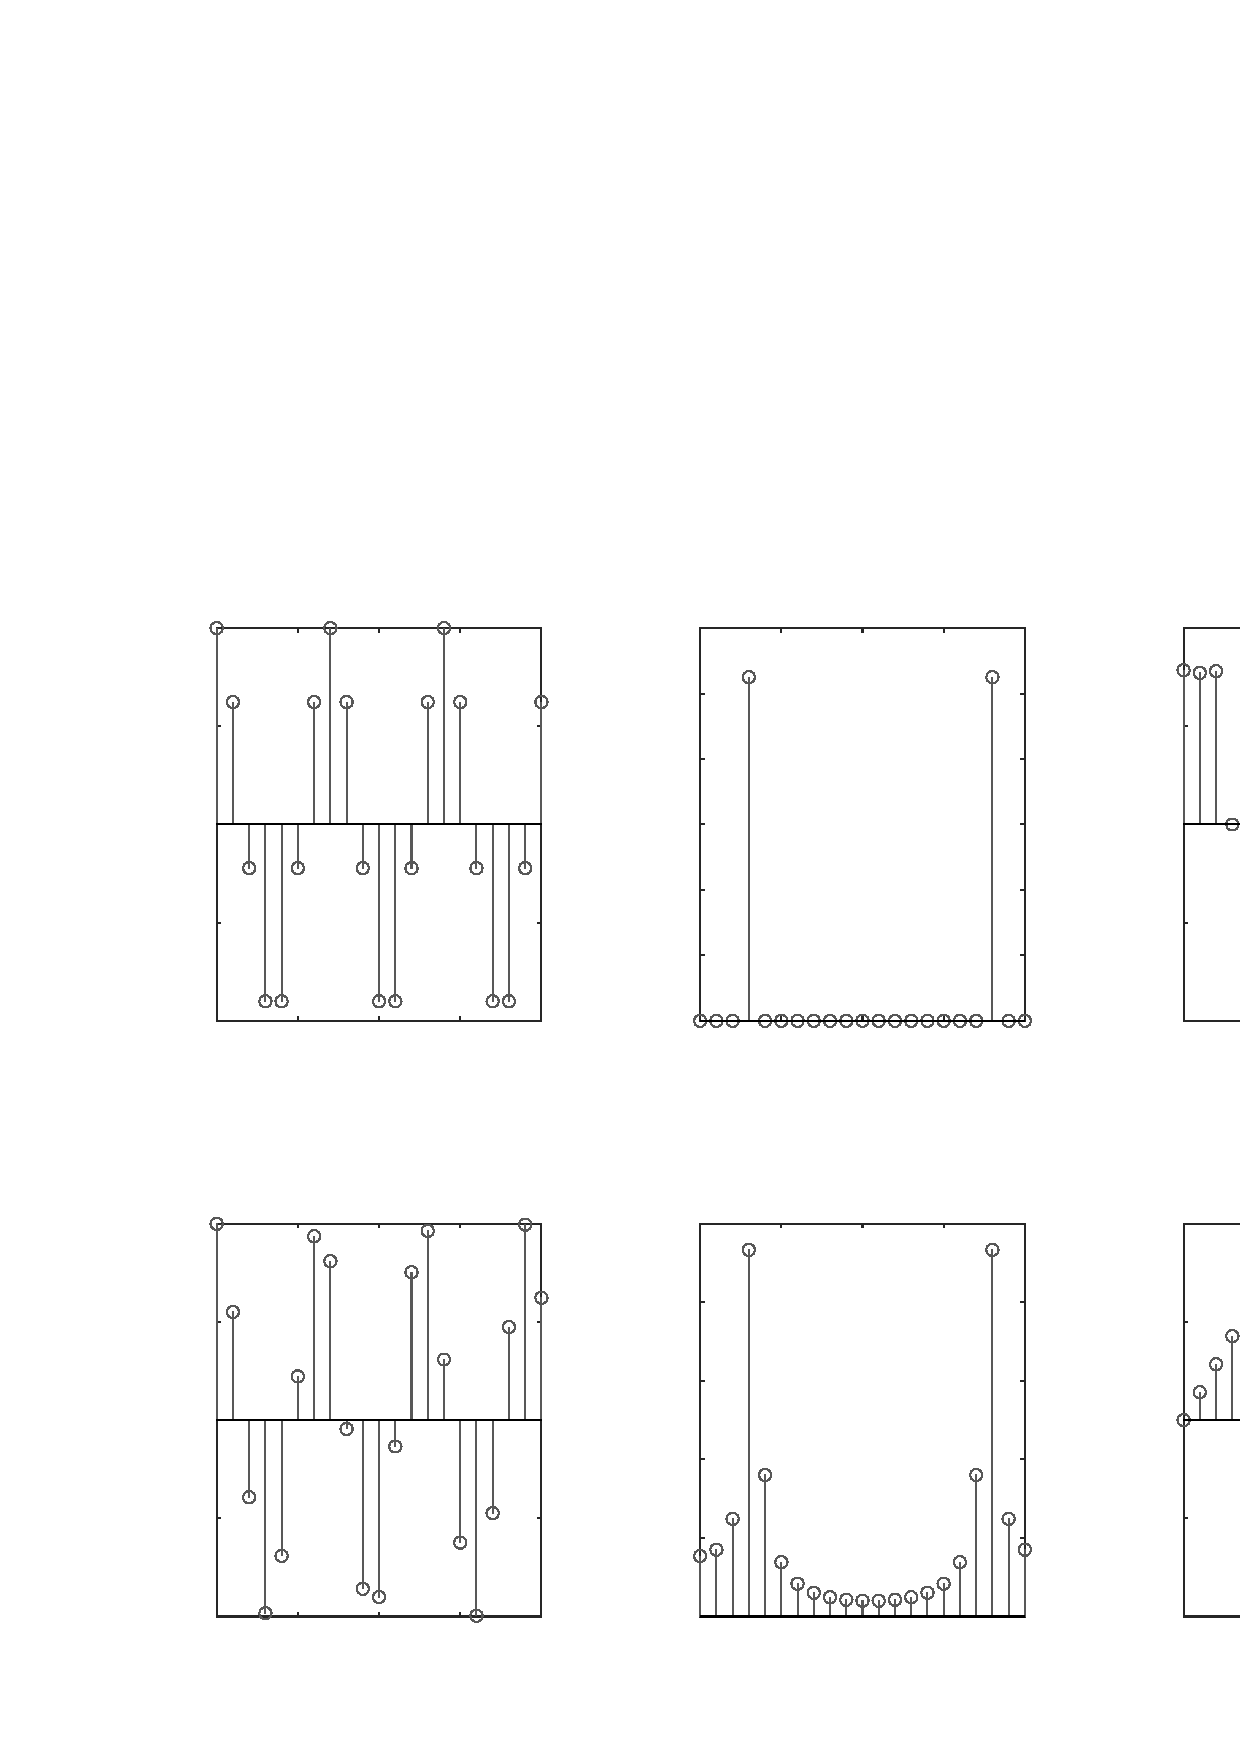
\includegraphics[scale=1]{octaves/dftCosine-inc}
\end{picture}%
\begin{picture}(800,600)(0,0)
\fontsize{13}{0}\selectfont\put(104,341.53){\makebox(0,0)[t]{\textcolor[rgb]{0.15,0.15,0.15}{{0}}}}
\fontsize{13}{0}\selectfont\put(142.97,341.53){\makebox(0,0)[t]{\textcolor[rgb]{0.15,0.15,0.15}{{5}}}}
\fontsize{13}{0}\selectfont\put(181.94,341.53){\makebox(0,0)[t]{\textcolor[rgb]{0.15,0.15,0.15}{{10}}}}
\fontsize{13}{0}\selectfont\put(220.91,341.53){\makebox(0,0)[t]{\textcolor[rgb]{0.15,0.15,0.15}{{15}}}}
\fontsize{13}{0}\selectfont\put(259.88,341.53){\makebox(0,0)[t]{\textcolor[rgb]{0.15,0.15,0.15}{{20}}}}
\fontsize{13}{0}\selectfont\put(97.0579,351.924){\makebox(0,0)[r]{\textcolor[rgb]{0.15,0.15,0.15}{{-1}}}}
\fontsize{13}{0}\selectfont\put(97.0579,399.049){\makebox(0,0)[r]{\textcolor[rgb]{0.15,0.15,0.15}{{-0.5}}}}
\fontsize{13}{0}\selectfont\put(97.0579,446.174){\makebox(0,0)[r]{\textcolor[rgb]{0.15,0.15,0.15}{{0}}}}
\fontsize{13}{0}\selectfont\put(97.0579,493.299){\makebox(0,0)[r]{\textcolor[rgb]{0.15,0.15,0.15}{{0.5}}}}
\fontsize{13}{0}\selectfont\put(97.0579,540.424){\makebox(0,0)[r]{\textcolor[rgb]{0.15,0.15,0.15}{{1}}}}
\fontsize{15}{0}\selectfont\put(181.94,550.424){\makebox(0,0)[b]{\textcolor[rgb]{0,0,0}{{Original time-domain sequence}}}}
\fontsize{15}{0}\selectfont\put(68.0579,446.174){\rotatebox{90}{\makebox(0,0)[b]{\textcolor[rgb]{0.15,0.15,0.15}{{Amplitude}}}}}
\fontsize{15}{0}\selectfont\put(181.94,325.53){\makebox(0,0)[t]{\textcolor[rgb]{0.15,0.15,0.15}{{Time index n}}}}
\fontsize{13}{0}\selectfont\put(336.06,341.53){\makebox(0,0)[t]{\textcolor[rgb]{0.15,0.15,0.15}{{0}}}}
\fontsize{13}{0}\selectfont\put(375.03,341.53){\makebox(0,0)[t]{\textcolor[rgb]{0.15,0.15,0.15}{{5}}}}
\fontsize{13}{0}\selectfont\put(414,341.53){\makebox(0,0)[t]{\textcolor[rgb]{0.15,0.15,0.15}{{10}}}}
\fontsize{13}{0}\selectfont\put(452.97,341.53){\makebox(0,0)[t]{\textcolor[rgb]{0.15,0.15,0.15}{{15}}}}
\fontsize{13}{0}\selectfont\put(491.94,341.53){\makebox(0,0)[t]{\textcolor[rgb]{0.15,0.15,0.15}{{20}}}}
\fontsize{13}{0}\selectfont\put(329.118,351.924){\makebox(0,0)[r]{\textcolor[rgb]{0.15,0.15,0.15}{{0}}}}
\fontsize{13}{0}\selectfont\put(329.118,383.34){\makebox(0,0)[r]{\textcolor[rgb]{0.15,0.15,0.15}{{2}}}}
\fontsize{13}{0}\selectfont\put(329.118,414.757){\makebox(0,0)[r]{\textcolor[rgb]{0.15,0.15,0.15}{{4}}}}
\fontsize{13}{0}\selectfont\put(329.118,446.174){\makebox(0,0)[r]{\textcolor[rgb]{0.15,0.15,0.15}{{6}}}}
\fontsize{13}{0}\selectfont\put(329.118,477.59){\makebox(0,0)[r]{\textcolor[rgb]{0.15,0.15,0.15}{{8}}}}
\fontsize{13}{0}\selectfont\put(329.118,509.007){\makebox(0,0)[r]{\textcolor[rgb]{0.15,0.15,0.15}{{10}}}}
\fontsize{13}{0}\selectfont\put(329.118,540.424){\makebox(0,0)[r]{\textcolor[rgb]{0.15,0.15,0.15}{{12}}}}
\fontsize{15}{0}\selectfont\put(414,550.424){\makebox(0,0)[b]{\textcolor[rgb]{0,0,0}{{Magnitude, r = 3}}}}
\fontsize{15}{0}\selectfont\put(308.118,446.174){\rotatebox{90}{\makebox(0,0)[b]{\textcolor[rgb]{0.15,0.15,0.15}{{Magnitude}}}}}
\fontsize{15}{0}\selectfont\put(414,325.53){\makebox(0,0)[t]{\textcolor[rgb]{0.15,0.15,0.15}{{Frequency index k}}}}
\fontsize{13}{0}\selectfont\put(568.12,341.53){\makebox(0,0)[t]{\textcolor[rgb]{0.15,0.15,0.15}{{0}}}}
\fontsize{13}{0}\selectfont\put(607.09,341.53){\makebox(0,0)[t]{\textcolor[rgb]{0.15,0.15,0.15}{{5}}}}
\fontsize{13}{0}\selectfont\put(646.06,341.53){\makebox(0,0)[t]{\textcolor[rgb]{0.15,0.15,0.15}{{10}}}}
\fontsize{13}{0}\selectfont\put(685.03,341.53){\makebox(0,0)[t]{\textcolor[rgb]{0.15,0.15,0.15}{{15}}}}
\fontsize{13}{0}\selectfont\put(724,341.53){\makebox(0,0)[t]{\textcolor[rgb]{0.15,0.15,0.15}{{20}}}}
\fontsize{13}{0}\selectfont\put(561.178,351.924){\makebox(0,0)[r]{\textcolor[rgb]{0.15,0.15,0.15}{{-4}}}}
\fontsize{13}{0}\selectfont\put(561.178,399.049){\makebox(0,0)[r]{\textcolor[rgb]{0.15,0.15,0.15}{{-2}}}}
\fontsize{13}{0}\selectfont\put(561.178,446.174){\makebox(0,0)[r]{\textcolor[rgb]{0.15,0.15,0.15}{{0}}}}
\fontsize{13}{0}\selectfont\put(561.178,493.299){\makebox(0,0)[r]{\textcolor[rgb]{0.15,0.15,0.15}{{2}}}}
\fontsize{13}{0}\selectfont\put(561.178,540.424){\makebox(0,0)[r]{\textcolor[rgb]{0.15,0.15,0.15}{{4}}}}
\fontsize{15}{0}\selectfont\put(646.06,550.424){\makebox(0,0)[b]{\textcolor[rgb]{0,0,0}{{Phase, r = 3}}}}
\fontsize{15}{0}\selectfont\put(543.178,446.174){\rotatebox{90}{\makebox(0,0)[b]{\textcolor[rgb]{0.15,0.15,0.15}{{Phase}}}}}
\fontsize{15}{0}\selectfont\put(646.06,325.53){\makebox(0,0)[t]{\textcolor[rgb]{0.15,0.15,0.15}{{Frequency index k}}}}
\fontsize{13}{0}\selectfont\put(104,55.6063){\makebox(0,0)[t]{\textcolor[rgb]{0.15,0.15,0.15}{{0}}}}
\fontsize{13}{0}\selectfont\put(142.97,55.6063){\makebox(0,0)[t]{\textcolor[rgb]{0.15,0.15,0.15}{{5}}}}
\fontsize{13}{0}\selectfont\put(181.94,55.6063){\makebox(0,0)[t]{\textcolor[rgb]{0.15,0.15,0.15}{{10}}}}
\fontsize{13}{0}\selectfont\put(220.91,55.6063){\makebox(0,0)[t]{\textcolor[rgb]{0.15,0.15,0.15}{{15}}}}
\fontsize{13}{0}\selectfont\put(259.88,55.6063){\makebox(0,0)[t]{\textcolor[rgb]{0.15,0.15,0.15}{{20}}}}
\fontsize{13}{0}\selectfont\put(97.0579,66){\makebox(0,0)[r]{\textcolor[rgb]{0.15,0.15,0.15}{{-1}}}}
\fontsize{13}{0}\selectfont\put(97.0579,113.125){\makebox(0,0)[r]{\textcolor[rgb]{0.15,0.15,0.15}{{-0.5}}}}
\fontsize{13}{0}\selectfont\put(97.0579,160.25){\makebox(0,0)[r]{\textcolor[rgb]{0.15,0.15,0.15}{{0}}}}
\fontsize{13}{0}\selectfont\put(97.0579,207.375){\makebox(0,0)[r]{\textcolor[rgb]{0.15,0.15,0.15}{{0.5}}}}
\fontsize{13}{0}\selectfont\put(97.0579,254.5){\makebox(0,0)[r]{\textcolor[rgb]{0.15,0.15,0.15}{{1}}}}
\fontsize{15}{0}\selectfont\put(181.94,264.5){\makebox(0,0)[b]{\textcolor[rgb]{0,0,0}{{Original time-domain sequence}}}}
\fontsize{15}{0}\selectfont\put(68.0579,160.25){\rotatebox{90}{\makebox(0,0)[b]{\textcolor[rgb]{0.15,0.15,0.15}{{Amplitude}}}}}
\fontsize{15}{0}\selectfont\put(181.94,39.6063){\makebox(0,0)[t]{\textcolor[rgb]{0.15,0.15,0.15}{{Time index n}}}}
\fontsize{13}{0}\selectfont\put(336.06,55.6063){\makebox(0,0)[t]{\textcolor[rgb]{0.15,0.15,0.15}{{0}}}}
\fontsize{13}{0}\selectfont\put(375.03,55.6063){\makebox(0,0)[t]{\textcolor[rgb]{0.15,0.15,0.15}{{5}}}}
\fontsize{13}{0}\selectfont\put(414,55.6063){\makebox(0,0)[t]{\textcolor[rgb]{0.15,0.15,0.15}{{10}}}}
\fontsize{13}{0}\selectfont\put(452.97,55.6063){\makebox(0,0)[t]{\textcolor[rgb]{0.15,0.15,0.15}{{15}}}}
\fontsize{13}{0}\selectfont\put(491.94,55.6063){\makebox(0,0)[t]{\textcolor[rgb]{0.15,0.15,0.15}{{20}}}}
\fontsize{13}{0}\selectfont\put(329.118,66){\makebox(0,0)[r]{\textcolor[rgb]{0.15,0.15,0.15}{{0}}}}
\fontsize{13}{0}\selectfont\put(329.118,103.7){\makebox(0,0)[r]{\textcolor[rgb]{0.15,0.15,0.15}{{2}}}}
\fontsize{13}{0}\selectfont\put(329.118,141.4){\makebox(0,0)[r]{\textcolor[rgb]{0.15,0.15,0.15}{{4}}}}
\fontsize{13}{0}\selectfont\put(329.118,179.1){\makebox(0,0)[r]{\textcolor[rgb]{0.15,0.15,0.15}{{6}}}}
\fontsize{13}{0}\selectfont\put(329.118,216.8){\makebox(0,0)[r]{\textcolor[rgb]{0.15,0.15,0.15}{{8}}}}
\fontsize{13}{0}\selectfont\put(329.118,254.5){\makebox(0,0)[r]{\textcolor[rgb]{0.15,0.15,0.15}{{10}}}}
\fontsize{15}{0}\selectfont\put(414,264.5){\makebox(0,0)[b]{\textcolor[rgb]{0,0,0}{{Magnitude, r = 3.3}}}}
\fontsize{15}{0}\selectfont\put(308.118,160.25){\rotatebox{90}{\makebox(0,0)[b]{\textcolor[rgb]{0.15,0.15,0.15}{{Magnitude}}}}}
\fontsize{15}{0}\selectfont\put(414,39.6063){\makebox(0,0)[t]{\textcolor[rgb]{0.15,0.15,0.15}{{Frequency index k}}}}
\fontsize{13}{0}\selectfont\put(568.12,55.6063){\makebox(0,0)[t]{\textcolor[rgb]{0.15,0.15,0.15}{{0}}}}
\fontsize{13}{0}\selectfont\put(607.09,55.6063){\makebox(0,0)[t]{\textcolor[rgb]{0.15,0.15,0.15}{{5}}}}
\fontsize{13}{0}\selectfont\put(646.06,55.6063){\makebox(0,0)[t]{\textcolor[rgb]{0.15,0.15,0.15}{{10}}}}
\fontsize{13}{0}\selectfont\put(685.03,55.6063){\makebox(0,0)[t]{\textcolor[rgb]{0.15,0.15,0.15}{{15}}}}
\fontsize{13}{0}\selectfont\put(724,55.6063){\makebox(0,0)[t]{\textcolor[rgb]{0.15,0.15,0.15}{{20}}}}
\fontsize{13}{0}\selectfont\put(561.178,66){\makebox(0,0)[r]{\textcolor[rgb]{0.15,0.15,0.15}{{-2}}}}
\fontsize{13}{0}\selectfont\put(561.178,113.125){\makebox(0,0)[r]{\textcolor[rgb]{0.15,0.15,0.15}{{-1}}}}
\fontsize{13}{0}\selectfont\put(561.178,160.25){\makebox(0,0)[r]{\textcolor[rgb]{0.15,0.15,0.15}{{0}}}}
\fontsize{13}{0}\selectfont\put(561.178,207.375){\makebox(0,0)[r]{\textcolor[rgb]{0.15,0.15,0.15}{{1}}}}
\fontsize{13}{0}\selectfont\put(561.178,254.5){\makebox(0,0)[r]{\textcolor[rgb]{0.15,0.15,0.15}{{2}}}}
\fontsize{15}{0}\selectfont\put(646.06,264.5){\makebox(0,0)[b]{\textcolor[rgb]{0,0,0}{{Phase, r = 3.3}}}}
\fontsize{15}{0}\selectfont\put(543.178,160.25){\rotatebox{90}{\makebox(0,0)[b]{\textcolor[rgb]{0.15,0.15,0.15}{{Phase}}}}}
\fontsize{15}{0}\selectfont\put(646.06,39.6063){\makebox(0,0)[t]{\textcolor[rgb]{0.15,0.15,0.15}{{Frequency index k}}}}
\end{picture}

}\caption{Plots of original signal (left), magnitude (center) and phase (right) of the Discrete Fourier Transform of sequence $\cos{2\pi r \frac{n}{N}}$. Notice how two perfect impulses are generated if and only if the quantity $r$ is an integer.}\label{oct:dftCosine}
\end{center}
\end{figure*}

The Discrete Fourier Transform of a cosine wave will produce a peculiar \emph{pair of impulses} located at the very same frequency of the sinusoid, provided the multiplying factor of $n$ is a \emph{multiple of $2\pi$}---that is, when $r \in \Z$. In all other cases, imperfect impulses will be generated, a phenomenon that is quite visible in Figure~\ref{oct:dftCosine} for the case of $r=3.3$.

The DFT of the delta impulse can be produced by running the following \texttt{octave} code, that will first generate three pictures like those in Figure~\ref{oct:dftCosine} related to a $\delta[n]$ sequence, then it will do the same with a delayed delta impulse,
\begin{verbatim}
N = 21;
M = 21;
u = [1 zeros(1,N-1)];
U = fft(u,M);
figure(1);
subplot(2,3,1);   n = 0:1:N-1;   stem(n,u);
title('Impulse in zero');
xlabel('Time index n'); ylabel('Amplitude')
subplot(2,3,2);   k = 0:1:M-1;   stem(k,abs(U));
title('Magnitude');
xlabel('Frequency index k'); ylabel('Magnitude')
subplot(2,3,3);   stem(k,angle(U));
title('Phase');
xlabel('Frequency index k'); ylabel('Phase')
\end{verbatim}

\begin{verbatim}
u = [zeros(1,4) 1 zeros(1,N-5)];
U = fft(u,M);
subplot(2,3,4);   n = 0:1:N-1;   stem(n,u);
title('Delayed impulse');
xlabel('Time index n'); ylabel('Amplitude')
subplot(2,3,5);   k = 0:1:M-1;   stem(k,abs(U));
title('Magnitude');
xlabel('Frequency index k'); ylabel('Magnitude')
subplot(2,3,6);   stem(k,angle(U));
title('Phase');
xlabel('Frequency index k'); ylabel('Phase')
\end{verbatim}



\begin{figure*}[ht]
\begin{center}
\scalebox{0.6}{
% Title: gl2ps_renderer figure
% Creator: GL2PS 1.4.2, (C) 1999-2020 C. Geuzaine
% For: Octave
% CreationDate: Wed Oct 19 16:35:19 2022
\setlength{\unitlength}{1pt}
\begin{picture}(0,0)
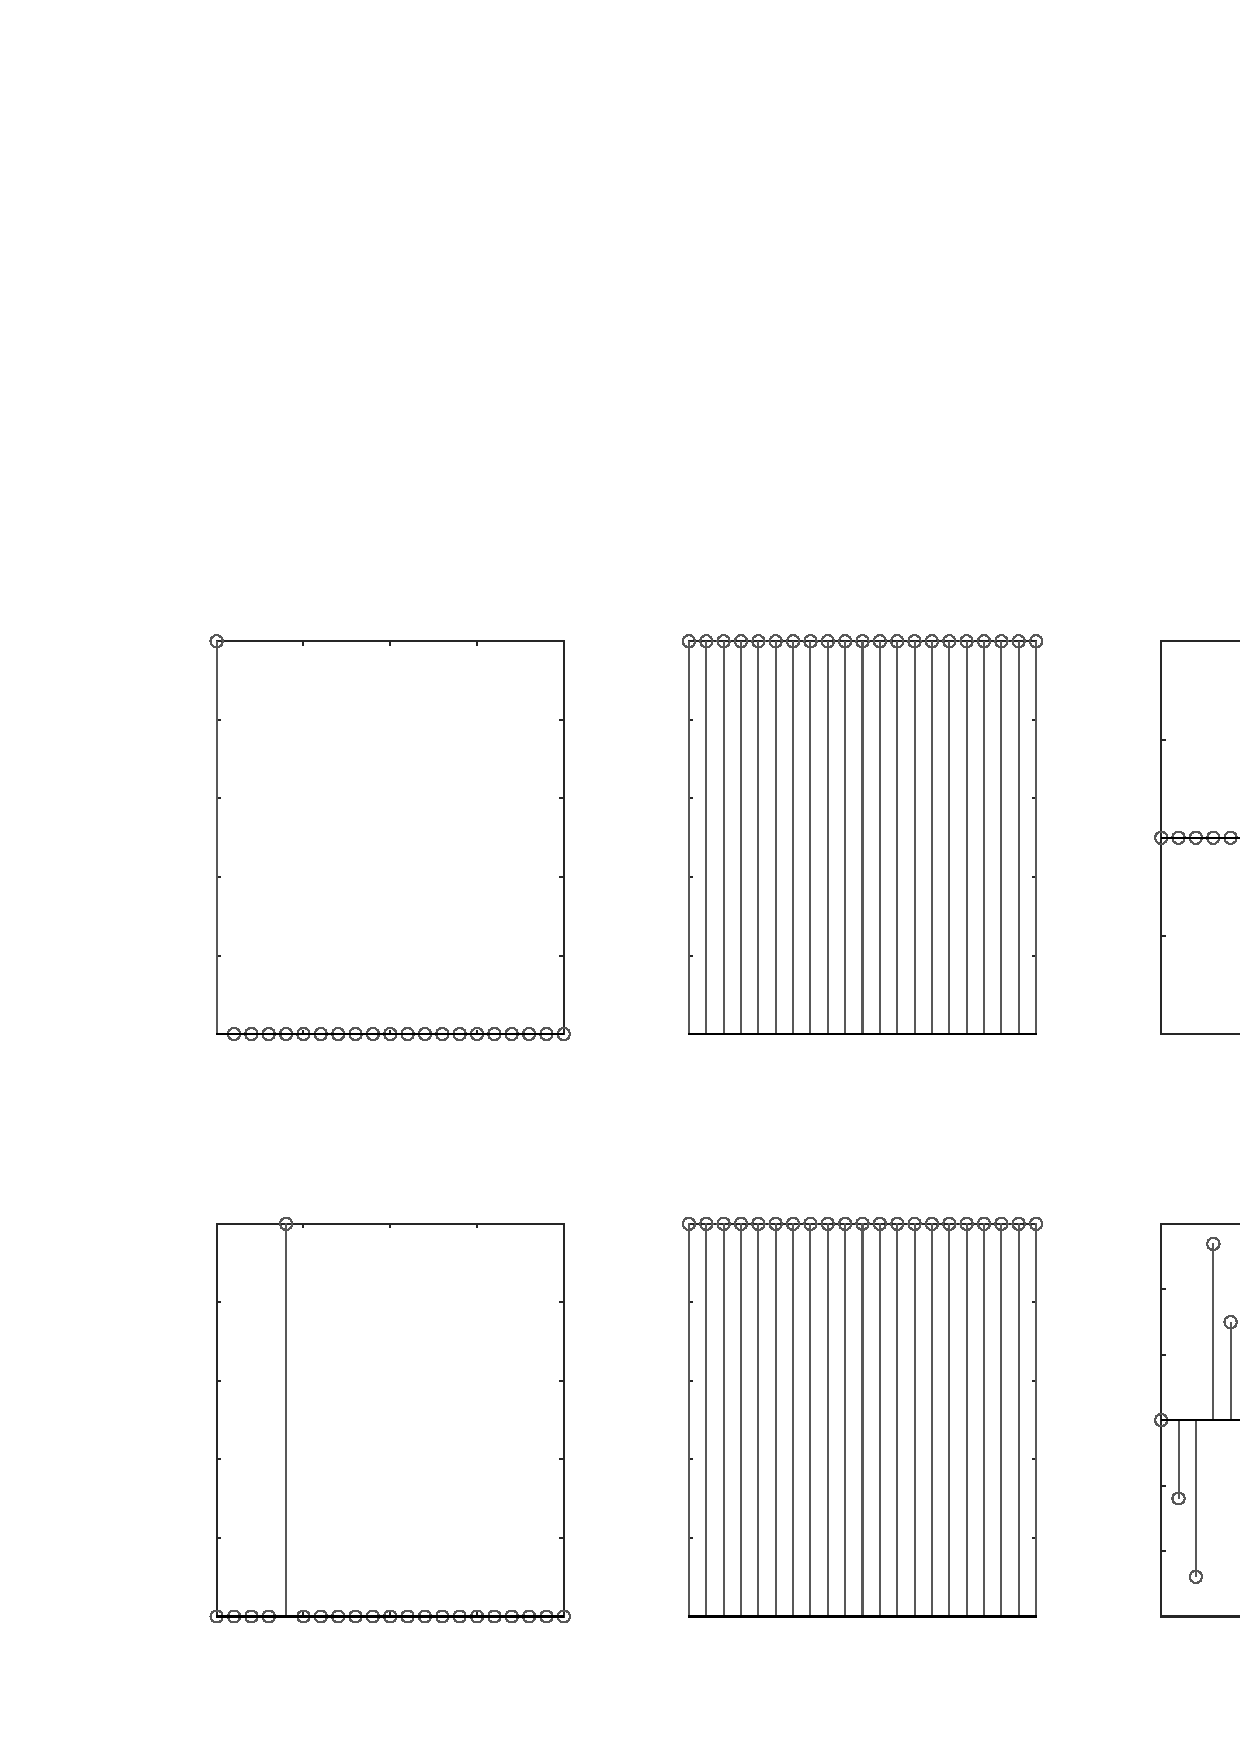
\includegraphics[scale=1]{octaves/dftImpulse-inc}
\end{picture}%
\begin{picture}(800,600)(0,0)
\fontsize{13}{0}\selectfont\put(104,335.173){\makebox(0,0)[t]{\textcolor[rgb]{0.15,0.15,0.15}{{0}}}}
\fontsize{13}{0}\selectfont\put(145.658,335.173){\makebox(0,0)[t]{\textcolor[rgb]{0.15,0.15,0.15}{{5}}}}
\fontsize{13}{0}\selectfont\put(187.316,335.173){\makebox(0,0)[t]{\textcolor[rgb]{0.15,0.15,0.15}{{10}}}}
\fontsize{13}{0}\selectfont\put(228.973,335.173){\makebox(0,0)[t]{\textcolor[rgb]{0.15,0.15,0.15}{{15}}}}
\fontsize{13}{0}\selectfont\put(270.631,335.173){\makebox(0,0)[t]{\textcolor[rgb]{0.15,0.15,0.15}{{20}}}}
\fontsize{13}{0}\selectfont\put(97.0679,345.566){\makebox(0,0)[r]{\textcolor[rgb]{0.15,0.15,0.15}{{0}}}}
\fontsize{13}{0}\selectfont\put(97.0679,383.266){\makebox(0,0)[r]{\textcolor[rgb]{0.15,0.15,0.15}{{0.2}}}}
\fontsize{13}{0}\selectfont\put(97.0679,420.966){\makebox(0,0)[r]{\textcolor[rgb]{0.15,0.15,0.15}{{0.4}}}}
\fontsize{13}{0}\selectfont\put(97.0679,458.666){\makebox(0,0)[r]{\textcolor[rgb]{0.15,0.15,0.15}{{0.6}}}}
\fontsize{13}{0}\selectfont\put(97.0679,496.366){\makebox(0,0)[r]{\textcolor[rgb]{0.15,0.15,0.15}{{0.8}}}}
\fontsize{13}{0}\selectfont\put(97.0679,534.066){\makebox(0,0)[r]{\textcolor[rgb]{0.15,0.15,0.15}{{1}}}}
\fontsize{15}{0}\selectfont\put(187.316,319.173){\makebox(0,0)[t]{\textcolor[rgb]{0.15,0.15,0.15}{{Time index n}}}}
\fontsize{15}{0}\selectfont\put(73.0679,439.816){\rotatebox{90}{\makebox(0,0)[b]{\textcolor[rgb]{0.15,0.15,0.15}{{Amplitude}}}}}
\fontsize{15}{0}\selectfont\put(187.316,544.066){\makebox(0,0)[b]{\textcolor[rgb]{0,0,0}{{Impulse in zero}}}}
\fontsize{13}{0}\selectfont\put(330.684,335.173){\makebox(0,0)[t]{\textcolor[rgb]{0.15,0.15,0.15}{{0}}}}
\fontsize{13}{0}\selectfont\put(372.342,335.173){\makebox(0,0)[t]{\textcolor[rgb]{0.15,0.15,0.15}{{5}}}}
\fontsize{13}{0}\selectfont\put(414,335.173){\makebox(0,0)[t]{\textcolor[rgb]{0.15,0.15,0.15}{{10}}}}
\fontsize{13}{0}\selectfont\put(455.658,335.173){\makebox(0,0)[t]{\textcolor[rgb]{0.15,0.15,0.15}{{15}}}}
\fontsize{13}{0}\selectfont\put(497.316,335.173){\makebox(0,0)[t]{\textcolor[rgb]{0.15,0.15,0.15}{{20}}}}
\fontsize{13}{0}\selectfont\put(323.752,345.566){\makebox(0,0)[r]{\textcolor[rgb]{0.15,0.15,0.15}{{0}}}}
\fontsize{13}{0}\selectfont\put(323.752,383.266){\makebox(0,0)[r]{\textcolor[rgb]{0.15,0.15,0.15}{{0.2}}}}
\fontsize{13}{0}\selectfont\put(323.752,420.966){\makebox(0,0)[r]{\textcolor[rgb]{0.15,0.15,0.15}{{0.4}}}}
\fontsize{13}{0}\selectfont\put(323.752,458.666){\makebox(0,0)[r]{\textcolor[rgb]{0.15,0.15,0.15}{{0.6}}}}
\fontsize{13}{0}\selectfont\put(323.752,496.366){\makebox(0,0)[r]{\textcolor[rgb]{0.15,0.15,0.15}{{0.8}}}}
\fontsize{13}{0}\selectfont\put(323.752,534.066){\makebox(0,0)[r]{\textcolor[rgb]{0.15,0.15,0.15}{{1}}}}
\fontsize{15}{0}\selectfont\put(414,319.173){\makebox(0,0)[t]{\textcolor[rgb]{0.15,0.15,0.15}{{Frequency index k}}}}
\fontsize{15}{0}\selectfont\put(299.752,439.816){\rotatebox{90}{\makebox(0,0)[b]{\textcolor[rgb]{0.15,0.15,0.15}{{Magnitude}}}}}
\fontsize{15}{0}\selectfont\put(414,544.066){\makebox(0,0)[b]{\textcolor[rgb]{0,0,0}{{Magnitude}}}}
\fontsize{13}{0}\selectfont\put(557.369,335.173){\makebox(0,0)[t]{\textcolor[rgb]{0.15,0.15,0.15}{{0}}}}
\fontsize{13}{0}\selectfont\put(599.027,335.173){\makebox(0,0)[t]{\textcolor[rgb]{0.15,0.15,0.15}{{5}}}}
\fontsize{13}{0}\selectfont\put(640.684,335.173){\makebox(0,0)[t]{\textcolor[rgb]{0.15,0.15,0.15}{{10}}}}
\fontsize{13}{0}\selectfont\put(682.342,335.173){\makebox(0,0)[t]{\textcolor[rgb]{0.15,0.15,0.15}{{15}}}}
\fontsize{13}{0}\selectfont\put(724,335.173){\makebox(0,0)[t]{\textcolor[rgb]{0.15,0.15,0.15}{{20}}}}
\fontsize{13}{0}\selectfont\put(550.437,345.566){\makebox(0,0)[r]{\textcolor[rgb]{0.15,0.15,0.15}{{-1}}}}
\fontsize{13}{0}\selectfont\put(550.437,392.691){\makebox(0,0)[r]{\textcolor[rgb]{0.15,0.15,0.15}{{-0.5}}}}
\fontsize{13}{0}\selectfont\put(550.437,439.816){\makebox(0,0)[r]{\textcolor[rgb]{0.15,0.15,0.15}{{0}}}}
\fontsize{13}{0}\selectfont\put(550.437,486.941){\makebox(0,0)[r]{\textcolor[rgb]{0.15,0.15,0.15}{{0.5}}}}
\fontsize{13}{0}\selectfont\put(550.437,534.066){\makebox(0,0)[r]{\textcolor[rgb]{0.15,0.15,0.15}{{1}}}}
\fontsize{15}{0}\selectfont\put(640.684,319.173){\makebox(0,0)[t]{\textcolor[rgb]{0.15,0.15,0.15}{{Frequency index k}}}}
\fontsize{15}{0}\selectfont\put(521.437,439.816){\rotatebox{90}{\makebox(0,0)[b]{\textcolor[rgb]{0.15,0.15,0.15}{{Phase}}}}}
\fontsize{15}{0}\selectfont\put(640.684,544.066){\makebox(0,0)[b]{\textcolor[rgb]{0,0,0}{{Phase}}}}
\fontsize{13}{0}\selectfont\put(104,55.6063){\makebox(0,0)[t]{\textcolor[rgb]{0.15,0.15,0.15}{{0}}}}
\fontsize{13}{0}\selectfont\put(145.658,55.6063){\makebox(0,0)[t]{\textcolor[rgb]{0.15,0.15,0.15}{{5}}}}
\fontsize{13}{0}\selectfont\put(187.316,55.6063){\makebox(0,0)[t]{\textcolor[rgb]{0.15,0.15,0.15}{{10}}}}
\fontsize{13}{0}\selectfont\put(228.973,55.6063){\makebox(0,0)[t]{\textcolor[rgb]{0.15,0.15,0.15}{{15}}}}
\fontsize{13}{0}\selectfont\put(270.631,55.6063){\makebox(0,0)[t]{\textcolor[rgb]{0.15,0.15,0.15}{{20}}}}
\fontsize{13}{0}\selectfont\put(97.0679,66){\makebox(0,0)[r]{\textcolor[rgb]{0.15,0.15,0.15}{{0}}}}
\fontsize{13}{0}\selectfont\put(97.0679,103.7){\makebox(0,0)[r]{\textcolor[rgb]{0.15,0.15,0.15}{{0.2}}}}
\fontsize{13}{0}\selectfont\put(97.0679,141.4){\makebox(0,0)[r]{\textcolor[rgb]{0.15,0.15,0.15}{{0.4}}}}
\fontsize{13}{0}\selectfont\put(97.0679,179.1){\makebox(0,0)[r]{\textcolor[rgb]{0.15,0.15,0.15}{{0.6}}}}
\fontsize{13}{0}\selectfont\put(97.0679,216.8){\makebox(0,0)[r]{\textcolor[rgb]{0.15,0.15,0.15}{{0.8}}}}
\fontsize{13}{0}\selectfont\put(97.0679,254.5){\makebox(0,0)[r]{\textcolor[rgb]{0.15,0.15,0.15}{{1}}}}
\fontsize{15}{0}\selectfont\put(187.316,39.6063){\makebox(0,0)[t]{\textcolor[rgb]{0.15,0.15,0.15}{{Time index n}}}}
\fontsize{15}{0}\selectfont\put(73.0679,160.25){\rotatebox{90}{\makebox(0,0)[b]{\textcolor[rgb]{0.15,0.15,0.15}{{Amplitude}}}}}
\fontsize{15}{0}\selectfont\put(187.316,264.5){\makebox(0,0)[b]{\textcolor[rgb]{0,0,0}{{Delayed impulse}}}}
\fontsize{13}{0}\selectfont\put(330.684,55.6063){\makebox(0,0)[t]{\textcolor[rgb]{0.15,0.15,0.15}{{0}}}}
\fontsize{13}{0}\selectfont\put(372.342,55.6063){\makebox(0,0)[t]{\textcolor[rgb]{0.15,0.15,0.15}{{5}}}}
\fontsize{13}{0}\selectfont\put(414,55.6063){\makebox(0,0)[t]{\textcolor[rgb]{0.15,0.15,0.15}{{10}}}}
\fontsize{13}{0}\selectfont\put(455.658,55.6063){\makebox(0,0)[t]{\textcolor[rgb]{0.15,0.15,0.15}{{15}}}}
\fontsize{13}{0}\selectfont\put(497.316,55.6063){\makebox(0,0)[t]{\textcolor[rgb]{0.15,0.15,0.15}{{20}}}}
\fontsize{13}{0}\selectfont\put(323.752,66){\makebox(0,0)[r]{\textcolor[rgb]{0.15,0.15,0.15}{{0}}}}
\fontsize{13}{0}\selectfont\put(323.752,103.7){\makebox(0,0)[r]{\textcolor[rgb]{0.15,0.15,0.15}{{0.2}}}}
\fontsize{13}{0}\selectfont\put(323.752,141.4){\makebox(0,0)[r]{\textcolor[rgb]{0.15,0.15,0.15}{{0.4}}}}
\fontsize{13}{0}\selectfont\put(323.752,179.1){\makebox(0,0)[r]{\textcolor[rgb]{0.15,0.15,0.15}{{0.6}}}}
\fontsize{13}{0}\selectfont\put(323.752,216.8){\makebox(0,0)[r]{\textcolor[rgb]{0.15,0.15,0.15}{{0.8}}}}
\fontsize{13}{0}\selectfont\put(323.752,254.5){\makebox(0,0)[r]{\textcolor[rgb]{0.15,0.15,0.15}{{1}}}}
\fontsize{15}{0}\selectfont\put(414,39.6063){\makebox(0,0)[t]{\textcolor[rgb]{0.15,0.15,0.15}{{Frequency index k}}}}
\fontsize{15}{0}\selectfont\put(299.752,160.25){\rotatebox{90}{\makebox(0,0)[b]{\textcolor[rgb]{0.15,0.15,0.15}{{Magnitude}}}}}
\fontsize{15}{0}\selectfont\put(414,264.5){\makebox(0,0)[b]{\textcolor[rgb]{0,0,0}{{Magnitude}}}}
\fontsize{13}{0}\selectfont\put(557.369,55.6063){\makebox(0,0)[t]{\textcolor[rgb]{0.15,0.15,0.15}{{0}}}}
\fontsize{13}{0}\selectfont\put(599.027,55.6063){\makebox(0,0)[t]{\textcolor[rgb]{0.15,0.15,0.15}{{5}}}}
\fontsize{13}{0}\selectfont\put(640.684,55.6063){\makebox(0,0)[t]{\textcolor[rgb]{0.15,0.15,0.15}{{10}}}}
\fontsize{13}{0}\selectfont\put(682.342,55.6063){\makebox(0,0)[t]{\textcolor[rgb]{0.15,0.15,0.15}{{15}}}}
\fontsize{13}{0}\selectfont\put(724,55.6063){\makebox(0,0)[t]{\textcolor[rgb]{0.15,0.15,0.15}{{20}}}}
\fontsize{13}{0}\selectfont\put(550.437,66){\makebox(0,0)[r]{\textcolor[rgb]{0.15,0.15,0.15}{{-3}}}}
\fontsize{13}{0}\selectfont\put(550.437,97.4166){\makebox(0,0)[r]{\textcolor[rgb]{0.15,0.15,0.15}{{-2}}}}
\fontsize{13}{0}\selectfont\put(550.437,128.833){\makebox(0,0)[r]{\textcolor[rgb]{0.15,0.15,0.15}{{-1}}}}
\fontsize{13}{0}\selectfont\put(550.437,160.25){\makebox(0,0)[r]{\textcolor[rgb]{0.15,0.15,0.15}{{0}}}}
\fontsize{13}{0}\selectfont\put(550.437,191.667){\makebox(0,0)[r]{\textcolor[rgb]{0.15,0.15,0.15}{{1}}}}
\fontsize{13}{0}\selectfont\put(550.437,223.083){\makebox(0,0)[r]{\textcolor[rgb]{0.15,0.15,0.15}{{2}}}}
\fontsize{13}{0}\selectfont\put(550.437,254.5){\makebox(0,0)[r]{\textcolor[rgb]{0.15,0.15,0.15}{{3}}}}
\fontsize{15}{0}\selectfont\put(640.684,39.6063){\makebox(0,0)[t]{\textcolor[rgb]{0.15,0.15,0.15}{{Frequency index k}}}}
\fontsize{15}{0}\selectfont\put(532.437,160.25){\rotatebox{90}{\makebox(0,0)[b]{\textcolor[rgb]{0.15,0.15,0.15}{{Phase}}}}}
\fontsize{15}{0}\selectfont\put(640.684,264.5){\makebox(0,0)[b]{\textcolor[rgb]{0,0,0}{{Phase}}}}
\end{picture}

}\caption{Plots of original signal (left), magnitude (center) and phase (right) of the Discrete Fourier Transform of sequences $\delta[n]$ and $\delta[n-4]$. The magnitude of the DFT is a constant as the transform of a delta will be a constant.}\label{oct:dftImpulse}
\end{center}
\end{figure*}

\subsection{Sampling process of a Discrete Fourier Transform}

Consider a sequence $x[n]$ whose Discrete-time Fourier Transform is $X(e^{j\omega})$. In order to obtain the Discrete Fourier Transform, one has to sample the DTFT at equally spaced points $\omega_k = \frac{2k\pi}{N}$ with $0 \leq k \leq N-1$, developing the frequency samples $\{X(e^{j\omega_k})\}$---these frequency samples can be considered the $N$-point DFT $Y[k]$ whose $N$-point IDFT is a sequence $y[n]$ of length $N$. This is because sampling a Discrete-time Fourier Transform will result in a Discrete Fourier Transform \emph{provided} the sampling is applied in $N$ points. That way, \[\{X(e^{j\omega_k})\} = Y[k].\]
Now, since the Discrete-time Fourier Transform is, like in Equation~\ref{eqn:inverseDiscreteTimeFourierTransform}
\[
    X(e^{j\omega}) = \sum_{l=-\infty}^\infty x[l] e^{-j\omega l};
\]
this leads to
\begin{align*}
    Y[k]
    &=  X(e^{j\omega_k}) = X\left(e^{j2\pi \frac k N}\right)\\
    &= \sum_{l=-\infty}^\infty x[l] e^{-j2\pi \frac{kl}{N}}\\
    &= \sum_{l=-\infty}^\infty x[l]W_N^{kl}.
\end{align*}

The trick now is to compute the IDFT of $y[n]$ and substitute the just obtained expression for $Y[k]$. That is,
\begin{align*}
    y[n]
    &= \frac 1 N \sum_{k=0}^{N-1} Y[k] W_N^{-kn}\\
    &= \frac 1 N \sum_{k=0}^{N-1}\sum_{l=-\infty}^\infty x[l]W_N^{kl} W_N^{-kn}\\
    &= \sum_{l=-\infty}^\infty\left(\frac 1 N \sum_{k=0}^{N-1} x[l]W_N^{-k(n-l)}\right);
\end{align*}
by means of the following identity
\begin{equation}\label{eqn:dftWnPropertyTwo}
    \sum_{n=0}^{N-1}W_N^{-k(n-l)} = \left\{\begin{array}{ll} N, & l = n + mN, \\ 0, & \mbox{otherwise}\end{array}\right.
\end{equation}
which is analogous of~\ref{eqn:dftWnProperty}, one soon obtains the desired relation
\begin{equation}\label{eqn:dftInfiniteReplicas}
    y[n] = \sum_{m=-\infty}^{\infty} x[n + mN], 0 \leq n \leq N-1.
\end{equation}

This last result, expressed by Equation~\ref{eqn:dftInfiniteReplicas} implies that $y[n]$ is obtained from the original sequence $x[n]$ by adding an \emph{infinite number of shifted replicas} of it, with each replica shifted by an integer multiple of $N$ sampling instants and observing the sum only for the interval $0 \leq n \leq N-1$. It has been obtained by picking an original sequence $x[n]$, performing its Discrete-time Fourier Transform $X(e^{j\omega})$, sampling it in $N$ points $\omega_k = \frac{2k\pi}{N}$ with $0 \leq k \leq N-1$ and finally obtained by re\"arranging and substituting on formulas. The integer number $m$ determines the amount of shift any replica of $x[n]$ is subject to---value $m=0$ corresponds to the original signal, value $m=1$ corresponds to a shift of $N$ samples, $m=2$ yields a replica shifted by $2N$, and so on.

The concept of infinite replicas is related to the fact that, in order to compute the DFT of a signal, one conceptually has to first make the sequence $x[n]$ \emph{periodic} by adding infinite replicas of the very same signal to create a sequence $y[n] = \sum_{m=-\infty}^{\infty} x[n + mN],$ with $0 \leq n \leq N-1$, and then the DFT can be computed.

When applying Equation~\ref{eqn:dftInfiniteReplicas} to finite-length sequences, one assumes that the samples outside the specified range are all zeros (like in zero-padding). Hence, if $x[n]$ is a sequence of length $M$ with $M \leq N$, then the sequence $y[n] = x[n]$ for all values $0 \leq n \leq N-1$. This behavior results from the fact that $N$ samples are more than what is needed ($M$ samples are needed to describe the original sequence $x[n]$). On contrary, in the opposite case of $M > N$ there is a so called \emph{time-domain aliasing} of samples of the sequence $x[n]$ in generating $y[n]$, with the end result that $x[n]$ cannot be recovered anymore from $y[n]$.

Suppose one has the sequence
\[\{x[n]\} = \begin{Bmatrix} \underset{\uparrow}{0} & 1 & 2 & 3 & 4 & 5\end{Bmatrix}\]
of length $M=6$. By sampling its Discrete-time Fourier Transform $X(e^{j\omega})$ at samples $\omega_k = \frac{2\pi k}{4}, 0 \leq k \leq 3$ and then applying a $4$-point Discrete Fourier Transform to these samples, one gets the sequence $y[n]$
\[
    y[n] = x[n] + x[n+4] + x[n-4], 0 \leq n \leq 3
\]
that is
\[
    \{y[n]\} = \begin{Bmatrix}\underset{\uparrow}{4} & 6 & 2 & 3\end{Bmatrix}.
\]

It is clear that from this sequence it is impossible to recover the original sequence $x[n]$---this behavior is induced by the choice of $N=4$, less than what would be required $N\leq M = 6$ in order to recover the original sequence.

Let now
\[
    \{x[n]\} = \begin{Bmatrix} 3 & 4&  5&  6&  7\end{Bmatrix},
\]
a sequence of length $M=5$ and compute $y[n]$ for values of $N=5$, $N=7$ and $N=3$. One obtains that,
\begin{itemize}
    \item for $N=5$, the resulting sequence \begin{align*}\{y[n]\} &= \underbrace{\begin{Bmatrix} 3 & 4 & 5 & 6 & 7\end{Bmatrix}}_{m = 0} + \underbrace{\begin{Bmatrix} 0 & 0 & 0 & 0 & 0 \end{Bmatrix}}_{m=1}\\ &+ \underbrace{\begin{Bmatrix} 0 & 0 & 0 & 0 & 0 \end{Bmatrix}}_{m=2} +\dots,\end{align*} showing that the original sequence can be fully recovered from $m=0$;
    \item for $N=7$ the behavior is quite similar---resulting sequence will be \begin{align*}\{y[n]\} &= \underbrace{\begin{Bmatrix} 3 & 4 & 5 & 6 & 7 & 0 & 0\end{Bmatrix}}_{m = 0}\\ &+ \underbrace{\begin{Bmatrix} 0 & 0 & 0 & 0 & 0 & 0 & 0 \end{Bmatrix}}_{m=1}\\ &+ \underbrace{\begin{Bmatrix} 0 & 0 & 0 & 0 & 0 & 0 & 0 \end{Bmatrix}}_{m=2} +\dots,\end{align*} and again, the original sequence can be fully recovered from $m=0$;
    \item for $N=3$ the behavior drastically change, as the $N=3$ samples are insufficient against the length of $x[n]$ which is $M$. Indeed, one obtains \begin{align*} \{y[n]\} &= \underbrace{\begin{Bmatrix} 3 & 4 & 5\end{Bmatrix}}_{m=0} + \underbrace{\begin{Bmatrix} 6 & 7 & 0\end{Bmatrix}}_{m=1} + \underbrace{\begin{Bmatrix}0 & 0 & 0\end{Bmatrix}}_{m=2} + \dots\\ &= \begin{Bmatrix} 9 & 11 & 5 \end{Bmatrix},\end{align*} which implies aliasing as the end result is different from the original sequence $x[n]$.
\end{itemize}

The case relative to $N=7$ suggests that a Discrete Fourier Transform with \emph{higher sample rate} can be obtained by transforming a zero-padded $x[n]$. This is because they are basically equivalent as choosing $N=7, M=7$ with a zero-padded signal $x[n]$ in which the length has been increased from $M=5$ to $M=7$ by adding zeros to the right.


\subsection{Discrete-time Fourier Transform by interpolation of a DFT}

As a brief recap, an $N$-point Discrete Fourier Transform of a sequence $x[n]$ of length $N$ is quite simply the frequency samples of its Discrete-time Fourier Transform $X(e^{j\omega})$, evaluated at $N$ uniformly spaced points in frequency that are
\[
    \omega_k = 2\pi \frac k N, 0 \leq k \leq N-1.
\]

In the above case one can obtain the DFT from the DTFT by sampling it at some points; however, the contrary can be performed. In fact, an \emph{approximated} version of a Discrete-time Fourier Transform can be obtained by \emph{interpolation} of the Discrete Fourier Transform. This practical approach allows one to get an approximated version of the DTFT of a finite-length sequence by computing the DFT first, choosing a proper interpolation function, and finally interpolating the DFT to obtain the continuous-time Fourier Transform.

\subsubsection{Numerical computation}

Let $X(e^{j\omega})$ be the DTFT of a sequence $x[n]$ of length $N$---one wants to evaluate the DTFT at a dense grid of $M$ frequencies\footnote{
The dense grid of frequencies is one of the ways in which a computation of a continuous-domain function can occur with calculators. Since it is impossible to compute all the infinite points in a real number interval, it is often enough to compute a great number of them so that the computed function appears almost continuous.
} $\omega_k = 2\pi \frac k M, 0 \leq k \leq M-1$ where the quantity $M \gg N$. In formulas,
\begin{align*}
    X(e^{j\omega})
    &= \sum_{n=0}^{N-1} x[n] e^{-j\omega_k n}\\
    &= \sum_{n=0}^{N-1} x[n] e^{-j2\pi \frac{kn}{M}}.
\end{align*}

Now, the original sequence of length $N$; since $M\gg N$, in order to avoid aliasing phenomena, one has to define a new \emph{extended sequence} $x_e[n]$ whose length is $M$ and it is extended by zero-padding from sample $N$ to sample $M-1$:
\[
    x_e[n] =
\left\{
    \begin{array}{ll}
        x[n] & 0 \leq n \leq N-1\\
        0 & N \leq n \leq M-1
    \end{array}
\right.
\]

Thanks to this extension of the original sequence, the Discrete-time Fourier Transform can be expressed as
\[
    X(e^{j\omega}) = \sum_{n=0}^{M-1} x_e[n] e^{-j2\pi \frac{kn}{M}}.
\]

The DTFT $X(e^{j\omega})$ can essentially be thought as an $M$-point DFT $X_e[k]$ of the extended sequence $x_e[n]$ of length $M$. The latter DFT $X_e[k]$ can be computed ahead using the \emph{Fast Fourier Transform} algorithm if $M$ is conveniently chosen as an integer of power $2$, such as $M = 2^K, K \in N^+$.

On \textsc{Matlab} code, the function \texttt{freqz} employs the above approach to evaluate the frequency response at a prescribed set of frequencies of a DTFT, expressed as a rational function in $e^{-j\omega}$.

\subsection{Periodicity of the DFT and the IDFT}

Due to the periodic nature of the complex exponential, both the Discrete Fourier Transform and the Inverse Discrete Fourier Transform are \emph{periodic sequences}. Indeed,
\begin{align*}
    X[k+N]
    &:= \sum_{n=0}^{N-1} x_n e^{-j2\pi\frac{(k+N)n}{N}} \\
    &= \sum_{n=0}^{N-1} x_n e^{-j2\pi\frac{kn}{N}}\underbrace{e^{-j2\pi n}}_{=1} \\
    &= \sum_{n=0}^{N-1} x_n e^{-j2\pi\frac{kn}{N}}\\
    &= X[k].
\end{align*}
and the inverse holds
\begin{align*}
    x[n+N]
    &= \frac 1 N \sum_{k=0}^{N-1}X[k] e^{j2\pi \frac{k(n+N)}{N}}\\
    &= \frac 1 N \sum_{k=0}^{N-1}X[k] e^{j2\pi \frac{kn}{N}}\underbrace{e^{j2\pi k}}_{=1}\\
    &= \frac 1 N \sum_{k=0}^{N-1}X[k] e^{j2\pi \frac{kn}{N}}\\
    &= x[n]
\end{align*}
showing off that both DFT and IDFT are periodic sequences of period $N$.

The above property is just the tip of the iceberg of a deeper rule, which is known as the \textbf{circular time-shifting property} of Discrete Fourier Transforms. We will encounter it later on.

\section{Overview of Fourier Transforms classes}

In general, Fourier Transforms can be divided in multiple classes. The following list indexes all possible cases related to various class of signals and their Fourier Transform.

\begin{itemize}
    \item \textbf{The sequence is continuous and aperiodic in the time domain}---then its Fourier Transform will be \emph{continuous and aperiodic} as well. In practice, this means that, given a signal $x_a(t)$, the Fourier Transform $X_a(f)$ will be
        \begin{equation}\label{eqn:fourierTransformContinuousAperiodic}
            X_a(f) = \int_{-\infty}^\infty x_a(t) e^{-j2\pi ft} dt,
        \end{equation}
        with its inverse transform of the form
        \begin{equation}\label{eqn:inverseFourierTransformContinuousAperiodic}
            x_a(t) = \int_{-\infty}^\infty X_a(f) e^{+j2\pi ft} df.
        \end{equation}
        The very same can be said of \emph{signals whose period is protracted for a very long time}, that is all signals that can be thought as ``almost aperiodic'' in the sense that they are remarkably far-reaching.
    \item \textbf{The sequence is continuous and periodic in the time domain}---then, its Fourier Transform will be \emph{discrete and aperiodic}. Its aperiodicity is inherited from the fact that the original signal is \emph{continuous}, just like in the previous case. Indeed, the formulas will be
        \begin{equation}\label{eqn:fourierTransformContinuousPeriodic}
            X[k] = \frac{1}{T_p}\int_{T_p} x_a(t) e^{-j2\pi kf_0t} dt,
        \end{equation}
        where the integration occurs in a portion of the signal that is the period $T_p$; its inverse transform will be of the form
        \begin{equation}\label{eqn:inverseFourierTransformContinuousPeriodic}
            x_a(t) = \sum_{k=-\infty}^\infty X[k] e^{+j2\pi kf_0t}.
        \end{equation}
        The value of $f_0$ is exactly the inverse of the length of the period $T_p$, that is $f_0 = \frac 1 {T_p}$. Veritably, in the case of signals whose period is far-reaching---that is, when $T_p$ is a lofty quantity---the frequency $f_0 \rightarrow 0$ as $T_p$ approaches infinity. Indeed, such transforms will resemble much and much more the continuous ones we find in the case of continuous aperiodic signals.
    \item \textbf{The sequence is discrete and aperiodic in the time domain}---then, its Fourier Transform is \emph{continuous and periodic}. This is the case of the Discrete-time Fourier Transform as in Equation~\ref{eqn:discreteTimeFourierTransform}, a ccase that is conceptually the dual of the \emph{discrete and aperiodic sequences} that lead to continuous and periodic transforms. In truth, in this case the formulas are actually the reverse, as
        \begin{equation}\label{eqn:fourierTransformDiscreteAperiodic}
            X(\omega) = \sum_{n=-\infty}^\infty x[n] e^{-j\omega n},
        \end{equation}
        \begin{equation}\label{eqn:inverseFourierTransformDiscreteAperiodic}
            x[n] = \frac{1}{2\pi}\int_{2\pi} X(\omega) e^{+j\omega n} d\omega.
        \end{equation}
        Noteworthily, the period for the Discrete-time Fourier Transform will be $2\pi$, as seen in~\ref{eqn:phasePrincipalValue}; undeniably, the integration is performed in a single period of $2\pi$.
    \item \textbf{The sequence is discrete and periodic in the time domain}---then, its Fourier Transform is \emph{discrete and periodic} as well. Undoubtedly, we are again facing the Discrete Fourier Transform as in Equation~\ref{eqn:discreteFourierTransform}. The formulas will for sure be
        \begin{equation}\label{eqn:fourierTransformDiscretePeriodic}
            X[k] = \sum_{n=0}^{N-1} x[n] e^{-j2\pi \frac{kn}{N}},
        \end{equation}
        \begin{equation}\label{eqn:inverseFourierTransformDiscretePeriodic}
            x[n] = \sum_{k=0}^{N-1} X[n] e^{+j2\pi \frac{kn}{N}},
        \end{equation}
        As already seen, there's a brawny relationship between the Discrete-time Fourier Transform and the Discrete Fourier Transform. As a matter of fact, the DFTF can be obtained by a DFT from an interpolation procedure; whilst the DFT can be obtained by sampling a DTFT.
\end{itemize}

To summarize concisely,
\begin{enumerate}
    \item from \textbf{continuous} signals one can only retrieve \textbf{aperiodic} transforms;
    \item \textbf{discrete} signals will yield \textbf{periodic} transforms;
    \item \textbf{aperiodic} signals will tally to \textbf{continuous} transforms;
    \item \textbf{periodic} signals will generate \textbf{discrete} transforms;
\end{enumerate}

If one pays adequate attention, can notice that there's a pattern comprised in the above rules, that is the following Table~\ref{tab:fourierTransformRules},
\begin{table}[ht]
\centering
\begin{tabular}{|l|c|l|}
    \hline
    \textbf{signal} & $\longleftrightarrow$ & \textbf{transform} \\
    \hline
    continuous & $\longleftrightarrow$ & aperiodic\\
    \hline
    discrete & $\longleftrightarrow$ & periodic\\
    \hline
    aperiodic & $\longleftrightarrow$ & continuous\\
    \hline
    periodic & $\longleftrightarrow$ & discrete\\
    \hline
\end{tabular}
\caption{Rules for retrieving the nature of the Fourier Transform based off the nature of the original signal--sequence.}\label{tab:fourierTransformRules}
\end{table}

Essentially, to determine the kind of Fourier Transform it is enough to look at the nature of the original signal--sequence and apply the above rules expressed in Table~\ref{tab:fourierTransformRules}. For instance, if $x$ is a \emph{discrete aperiodic} sequence, its Fourier Transform $X$ will be \emph{periodic continuous}. Analogously, let $x$ be a \emph{periodic discrete} sequence; its Fourier Transform $X$ will be \emph{discrete periodic} as well by applying the very same rules.

\section{Properties of Discrete Fourier Transforms}

Discrete Fourier Transforms share a lot of properties with the Discrete-time Fourier Transforms, its continuous counterpart. Some of these properties are essentially identical to those of the DTFT, while some others are different. A summary of the Discrete Fourier Transforms properties are given by the following Tables~\ref{tab:discreteFourierTransformPropertiesAndTheorems}, \ref{tab:discreteFourierTransformPropertiesAndTheorems2}~and~\ref{tab:discreteFourierTransformPropertiesAndTheorems3}. All properties refer to sequences of length $N$.

\begin{table*}[ht]
\centering
\begin{tabular}{c c}
    \hline
    \textbf{Sequence} & \textbf{Discrete Fourier Transform} \\
    \hline
    $x[n]$  & $X[k]$ \\
    \hline
    $x^*[\langle -n\rangle_N]$ & $X^*[k]$ \\
    $\Re{\{x[n]\}}$ & $X_{pcs}[k] = \frac 1 2 \{X[\langle k\rangle_N] + X^*[\langle -k \rangle_N]\}$\\
    $j\Im{\{x[n]\}}$ & $X_{pca}[k] = \frac 1 2 \{X[\langle k\rangle_N] - X^*[\langle -k\rangle_N]\}$\\
    $x_{pcs}[n]$ & $\Re{X[k]}$ \\
    $x_{pca}[n]$ & $j\Im{X[k]}$ \\
    \hline
\end{tabular}
\caption{Notable Discrete Fourier Transform properties. $x_{pcs}[k]$ and $X_{pca}[k]$ are the conjugate-symmetric and conjugate-antisymmetric parts of $x[k]$, respectively. Likewise, $X_{pcs}[k]$ and $X_{pca}[k]$ are, respectively, the conjugate-symmetric and conjugate-antisymmetric parts of $X[k]$. The expression $\langle -k \rangle_N$ denotes the \emph{modulo expression}---the sequence is periodic of period $N$. $X$ is periodic and of infinite length.}\label{tab:discreteFourierTransformPropertiesAndTheorems}
\end{table*}

\begin{table*}[ht]
\centering
\begin{tabular}{c c}
    \hline
    \textbf{Sequence} & \textbf{Discrete Fourier Transform} \\
    \hline
    $x[n]$ & $X[k] = \Re{X[k]} + j\Im{X[k]}$ \\
    \hline
    $x_{pe}[n]$ & $\Re{X[k]}$ \\
    $x_{po}[n]$ & $j\Im {X[k]}$ \\
    \hline
    Symmetry relations & $X[k] = X^*[\langle -k\rangle_N]$ \\
    --- & $\Re X[k] = \Re X[\langle -l\rangle_N]$ \\
    --- & $\Im X[k] = -\Im X[\langle -l \rangle_N]$ \\
    --- & $|X[k]| = |X[\langle -l \rangle_N]|$ \\
    --- & $\arg{X[k]} = -\arg{X[\langle -l \rangle_N]}$ \\
    \hline
\end{tabular}
\caption{Notable Discrete Fourier Transform properties. Sequences $x_{pe}[n]$ and $x_{po}[n]$ are, respectively, the even and the odd parts of the sequence $x[n]$. In the above table, $x[n]$ is a real sequence.}\label{tab:discreteFourierTransformPropertiesAndTheorems2}
\end{table*}

\begin{table*}[ht]
\centering
\begin{tabular}{ccc}
    \hline
    \textbf{Name} & \textbf{Sequence} & \textbf{Discrete Fourier Transform} \\
    \hline
    Linearity & $\alpha g[n] + \beta h[n]$ & $\alpha G[k] + \beta H[k]$\\
    Circular time-shifting & $g[\langle n-n_0\rangle_N]$ & $W_N^{kn_0} G[k]$ \\
    Circular frequency-shifting & $W_N^{-kn_0}g[n]$ & $G[\langle k - k_0 \rangle_N]$ \\
    Duality & $G[n]$ & $Ng[\langle -k \rangle_N]$ \\
    Circular $N$-point convolution & $\sum_{m=0}^{N-1} g[m] h[\langle n - m \rangle_N]$ &$ G[k] \cdot H[k]$\\
    Modulation & $g[n] \cdot h[n]$ &$ \frac{1}{N} \sum:{m=0}^{N-1} G[k] \cdot H[\langle k - m\rangle_N]$\\
    \hline
    Parseval's relation & $\sum_{n=-\infty}^\infty g[n]h^*[n]$ &$= \frac 1 {2\pi} \int_{-\pi}^\pi G(e^{j\omega})H^*(e^{j\omega})d\omega$\\
    \hline
\end{tabular}
\caption{Notable Discrete Fourier Transform properties. Notice how the properties---set side by side to those of Table~\ref{tab:discreteTimeFourierTransformPropertiesAndTheorems3} are now \emph{circular} properties that make use of the modulo operation.}\label{tab:discreteFourierTransformPropertiesAndTheorems3}
\end{table*}

\section{Circular operations on finite-length sequences}

Finite-length sequences have distinctive traits for which a special care is required. In particular, common operations such as time-shifting, time-reversal and convolutions have to be conceived diversely. I'm referring in particular to all operations which \emph{modify} the domain of the original signal---let's say, $0 \leq n \leq N-1$---by producing a result whose domain is \emph{different} from $0 \leq n \leq N-1$. Since the Discrete Fourier Transform is periodic with the \emph{same} period of the original signal, one wants to avoid to modify the domain of the resulting signal with any operation.

Contemplate a length-$N$ sequence $x[n]$, defined for samples $0\leq n \leq N-1$. Its sample values are equal to zero for all samples before $0$ and after $N-1$, that is for $n < 0 \wedge n \leq N$. A \emph{time-reversal} operation on $x[n]$ would result in a sequence $x[-n]$ of length $N$, that is defined for time instants $-(N-1) \leq n \leq 0$. Furthermore, a \emph{linear time-shift} of $x[n]$ by a quantity $M \in \Z$ would result in a sequence $x[n+M]$ of length $N$, no longer defined for $0 \leq n \leq N-1$, but for $M \leq n \leq N-1 + M$. Correspondingly, a \emph{convolution sum} of two sequences of length $N$ defined for $0 \leq n \leq N-1$ would result in a sequence of length $2N + 1$, defined for $0 \leq n \leq 2N-2$---such that it is longer than the original sequences.

Yet, we would like to preserve both the \emph{exact length} of the sequence and \emph{its location in time instants}. For instance, we would like the output of operations to persist in the range $0 \leq n \leq N-1$. By this logic, the need to define new types of operations emerges---in particular, new operations analogous of time-reversal, time-shifting and convolution sum with the resultant sequences in the same range of the input sequences. The key to solve this issue are the \textbf{circular operations}.

\subsection{Modulo operation}
The time-reversal operation on a finite-length sequence is obtained by means of the \textbf{modulo operation}. Let $0,1,\dots, N-1$ be a set of $N$ positive integers and let $m \in \Z$ be any integer. The integer $r$ obtained by evaluating
\begin{equation}\label{eqn:moduloOperation}
    r = \langle m \rangle_N = m \mod N
\end{equation}
is called the \textbf{residue}. The residue $r$ is an integer whose value is between $0$ and $N-1$ (as the modulo operation yields). We will denote the modulo operation with the notation \[ \langle m \rangle_N = m \mod N. \] Due to modulo properties, if $r = \langle m \rangle_N$ then $r = m + lN$, where $l \in \Z$ such that $0 \leq m + lN \leq N-1$.
As an example, let $N=7$ and $m = 25$: one has
\[
    r = 25 + 7l = 25 - 7 \times 3 = 4
\]
which means $\langle 25 \rangle_7 = 4$. Another example is $N=7$ and $m=-15$, for which
\[
    r = -15 + 7l = -15 + 7 \times 3 = 6
\]
and yields $\langle -15 \rangle_7 = 6$.

\subsection{Circular time-reversal operation}
Another operation we are going to find a substitute for is the \emph{time-reversal}---in practice, we are going to build the \textbf{circular time-reversal operation}.

Circular time-reversals grab the original sequence, and invert the order of the sequence by preserving the time instant at position $0$. The circular time-reversal $\{y[n]\}$ of $\{x[n]\}$ is a new sequence of length $N$ as well, thus defined for $0 \leq n \leq N-1$, given by the formula
\begin{equation}\label{eqn:circularTimeReversal}
    \{y[n]\} = \{x[\langle -n \rangle_N]\}.
\end{equation}
As an example, consider the sequence in Figure~\ref{tikz:circularTimeReversal}, where the original sequence is said to be \emph{circularly reversed}.
\begin{figure}[ht]
\begin{center}
    \begin{tikzpicture}
        \node[label=north:{Original sequence}] (original) at (0,0) {$\{x[n]\} = \begin{Bmatrix} x[0] & x[1] & x[2] & x[3] & x[4]\end{Bmatrix}$};
        \node[label=north:{Circular time-reversed sequence}] (original) at (0,-2) {$\{y[n]\} = \begin{Bmatrix} x[0] & x[4] & x[3] & x[2] & x[1]\end{Bmatrix}$};
        \draw[-stealth, thick] (-1.75,-0.45) -- (+3,-.45);
        \draw[-stealth, thick] (-1.35,-2.35) .. controls (-2.95,-3.45) and (+8.4,-2.25) .. (-.65,-2.35);
    \end{tikzpicture}
    \end{center}\caption{The \emph{circular time-reversal} technique. The output sequence is a reversed original copy, except for the sample at the origin which remains in place.}\label{tikz:circularTimeReversal}
\end{figure}

Basically, the circular time-reversal is a special kind of time-reversal in which the ``position'' from $0$ to $N-1$ of the original sequence is preserved, whilst its samples are almost totally reversed, with the sole exception of the sample at the origin. A sequence like
\[
    \begin{matrix} -1 & 7 & 5 & 9 & 4 & -12\end{matrix}
\]
the moment it is exposed to the circular time-reversal operation is remodeled into the sequence
\[
    \begin{matrix} -1 & -12 & 4 & 9 & 5 & 7\end{matrix}.
\]

\subsection{Circular shift operation}
As formerly mentioned, the time shifting operation has to be modified as well to fit our Discrete Fourier Transform signal processing. Sure thing, we might introduce the \textbf{circular shift} operation, defined using the modulo operation as in~\ref{eqn:moduloOperation} as well.

Let $x[n]$ be a sequence possessing length $N$, defined for $0 \leq n \leq N-1$---the \emph{circularly shifted by $n_0$ samples} version $x_c[n]$ is given by
\begin{equation}\label{eqn:circularShift}
    x_c[n] = x[\langle n - n_0 \rangle_N],
\end{equation}
with $x_c[n]$ also being a length-$N$ sequence defined for the same time instants $0\leq n \leq N-1$ as the original sequence. For $n_0 > 0$ one performs a \emph{right circular shift}---the above equation implies that the new sequence is defined as such
\[
    x_c[n] =
    \left\{
        \begin{array}{ll}
            x[n-n_0] & n_0 \leq n \leq N-1\\
            x[N- n-n_0] & 0 \leq n < n_0
        \end{array}
    \right.
\]

Figuring out the implications of the above system can be tricky---Figure~\ref{tikz:circularShift} helps with an illustration of what happens when a signal is circularly-shifted

\begin{figure}[ht]
\begin{center}
    \begin{tikzpicture}
        %\node[above,font=\large\bfseries] at (0,3.5) {Unit sample se\-quen\-ce};
        \draw[-stealth] (-.5,0) -- (1.6,0) node[anchor=north west] {$n$};

        \foreach \x in {0,1,...,5}
            \draw (\x*0.25 cm,1pt) -- (\x*0.25 cm,-1pt) node[anchor=north] {$\x$};
       
        \draw[-stealth] (-.25,1.6) .. controls (-.25,1.6) and (1.5,1.6) .. (1.5,1.6);
        \draw[-Circle] (0*0.25,0) -- (0*0.25,1*0.25);
        \draw[-Circle] (1*0.25,0) -- (1*0.25,2*0.25);
        \draw[-Circle] (2*0.25,0) -- (2*0.25,3*0.25);
        \draw[-Circle] (3*0.25,0) -- (3*0.25,4*0.25);
        \draw[-Circle] (4*0.25,0) -- (4*0.25,5*0.25);
        \draw[-Circle] (5*0.25,0) -- (5*0.25,6*0.25);
        \node[label=south:{Original}] (label) at (0.65,-.5) {};
        \node[label=south:{$x[n]$}] (labeltwo) at (0.65,-1) {};
    \end{tikzpicture}
    \begin{tikzpicture}
        %\node[above,font=\large\bfseries] at (0,3.5) {Unit sample se\-quen\-ce};
        \draw[-stealth] (-.5,0) -- (1.6,0) node[anchor=north west] {$n$};

        \foreach \x in {0,1,...,5}
            \draw (\x*0.25 cm,1pt) -- (\x*0.25 cm,-1pt) node[anchor=north] {$\x$};
       
        \draw[-stealth] (5*.25,1.6) .. controls (+1.25,1.6) and (1,1.9) .. (0,1.6);
        \draw[-stealth] (+.25,1.5) .. controls (+.25,1.5) and (1,1.5) .. (1,1.5);
        \draw[-Circle] (0*0.25,0) -- (0*0.25,6*0.25);
        \draw[-Circle] (1*0.25,0) -- (1*0.25,1*0.25);
        \draw[-Circle] (2*0.25,0) -- (2*0.25,2*0.25);
        \draw[-Circle] (3*0.25,0) -- (3*0.25,3*0.25);
        \draw[-Circle] (4*0.25,0) -- (4*0.25,4*0.25);
        \draw[-Circle] (5*0.25,0) -- (5*0.25,5*0.25);
        \node[label=south:{$x[\langle n-1\rangle_6]$}] (label) at (0.65,-.5) {};
        \node[label=south:{$x[\langle n+5\rangle_6]$}] (labeltwo) at (0.65,-1) {};
    \end{tikzpicture}
    \begin{tikzpicture}
        %\node[above,font=\large\bfseries] at (0,3.5) {Unit sample se\-quen\-ce};
        \draw[-stealth] (-.5,0) -- (1.6,0) node[anchor=north west] {$n$};

        \foreach \x in {0,1,...,5}
            \draw (\x*0.25 cm,1pt) -- (\x*0.25 cm,-1pt) node[anchor=north] {$\x$};
       
        \draw[-stealth] (1,1.5) .. controls (1,1.5) and (1.25,1.5) .. (1.25,1.5);
        \draw[-stealth] (5*.25,1.6) .. controls (+1.25,1.6) and (1,1.9) .. (0,1.6);
        \draw[-stealth] (0,1.5) .. controls (0,1.5) and (.65,1.5) .. (.65,1.5);
        \draw[-Circle] (0*0.25,0) -- (0*0.25,3*0.25);
        \draw[-Circle] (1*0.25,0) -- (1*0.25,4*0.25);
        \draw[-Circle] (2*0.25,0) -- (2*0.25,5*0.25);
        \draw[-Circle] (3*0.25,0) -- (3*0.25,6*0.25);
        \draw[-Circle] (4*0.25,0) -- (4*0.25,1*0.25);
        \draw[-Circle] (5*0.25,0) -- (5*0.25,2*0.25);
        \node[label=south:{$x[\langle n-4\rangle_6]$}] (label) at (0.65,-.5) {};
        \node[label=south:{$x[\langle n+2\rangle_6]$}] (labeltwo) at (0.65,-1) {};
    \end{tikzpicture}
\end{center}\caption{Circular shift operation on a ramp sequence of length $N = 6$. As the samples are pushed to the right, they ``come back'' from the left, realizing a circular pattern. Of course, the original sequence $x[n]$ is equal to a sequence $x[\langle n - 6\rangle_N] = x[n]$ that is circularly shifted of a quantity that is the same of its entire length, thanks to the modulo operation.}\label{tikz:circularShift}
\end{figure}

As can be seen from Figure~\ref{tikz:circularShift}, a right circular shift from $n_0$ is completely equivalent to a left circular shift by $N-n_0$ sample periods. As soon as we are performing a shift by means of the modulo operation, any circular shift by a quantity $n_g > N$ will be completely equivalent to a circular shift by $\langle n_g \rangle_N$, as any number greater than $N$ will be exposed to the modulo operation as in~\ref{eqn:moduloOperation}, causing the result to be still less than $N$. For instance, suppose one has a length-$11$ signal and wants to perform a circular shift by $n_g = 67$. What takes effect is that such shift will be completely equivalent to a shift $n_0 = \langle n_g \rangle_N$, that is
\[
    n_0 = \langle n_g \rangle_N = \langle 67 \rangle_{11} = 67 \mod 11 = 1
\]
completely comparable to a simple unit shift.

\subsection{Circular padding operation}
Yet another operation should be modified---the zero-padding operation, which would elseways alter the length of the original signal. In point of fact, the zero-padding operation \emph{actually means} altering the length of the original signal by adding a bunch of zeros to the left or to the right. Such an operation cannot deal proficiently in relation to the Discrete Fourier Transforms, since as we have earlier said the favored approach would be to preserve the characteristics of the original signal.

The implicit periodicity of the sequences manipulated with the Discrete Fourier Transform requires to substitute the \emph{zero-padding} operation with a \emph{circular padding} variant. This circular padding variant will reconstruct and remodel our input signal by periodicizing it, an operation that will pad our signal with \emph{as many replicas of the original sequance as needed} instead of padding with zeros. This means that instead of performing
\[
    \begin{Bmatrix} 1 & 2 & 3 & 4 \end{Bmatrix} \rightarrow \begin{Bmatrix} \cdots & 0 & 0 & 1 & 2 & 3 & 4 & 0 & 0 & \cdots\end{Bmatrix}
\]
one adds multiple replicas of the very same signal as from input. The operation is illustrated in Figure~\ref{tikz:circularZeroPadding}.

\begin{figure}[ht]
\begin{center}
    \begin{tikzpicture}
        \node[label=north:{Original sequence}] (original) at (0,0) {$\begin{bmatrix} 1 & 2 & 3 & 4\end{bmatrix}$};
        \node[label=north:{Padded sequence}] (chain) at (0,-2) {$\begin{bmatrix}\cdots & 1 & 2 & 3 & 4 & 1 & 2 & 3 & 4 & 1 & 2 & 3 & 4 & \cdots \end{bmatrix}$};
        \draw[-stealth] (0,-0.25) .. controls (0,-.75) and (-2,-1) .. (-2.15,-1.65);
        \draw[-stealth] (0,-0.25) .. controls (0,-.75) and (+2,-1) .. (+2.15,-1.65);
        \draw[-stealth] (0,-0.25) .. controls (0,-.75) and (-2.5,-1) .. (-3.25,-1.65);
        \draw[-stealth] (0,-0.25) .. controls (0,-.75) and (+2.5,-1) .. (+3.25,-1.65);
        \draw [thick, decorate, decoration = {calligraphic brace}] (0.5*2.2,-1.8) -- (0.5*5.9,-1.8);
        \draw [thick, decorate, decoration = {calligraphic brace}] (-0.5*5.9,-1.8) -- (-0.5*2.2,-1.8);
    \end{tikzpicture}
    \end{center}\caption{The \emph{circular padding} technique. Pay attention at how the pattern $\begin{bmatrix} 1 & 2 & 3 & 4 \end{bmatrix}$ is repeated indefinitely, to construct an infinite-length signal which repeats indefinitely with a period of the same length of the original signal---in this situation, $N=4$.}\label{tikz:circularZeroPadding}
\end{figure}

This way, one does not append an infinite number of zeros, but instead appends an infinite number of signal replicas before and after the original sequence. Of course, the resulting signal will virtually be of infinite length---still, it will be a periodic sequence.

The circular padding acts very well with the Discrete Fourier Transforms. When we have examined the Discrete Fourier Transform we figured out that the $N$-point Inverse Discrete Fourier Transform $y[n]$ as expressed by Equation~\ref{eqn:dftInfiniteReplicas} was akin to the original $N$-length sequence $x[n]$, but composed of \emph{infinite replicas} of the original sequence. Regardless of the fact that the DFT was attained with its original formula as in~\ref{eqn:discreteFourierTransform} or from sampling the Discrete-time Fourier Transform, as a matter of fact the inverse DFT is an infinite-length sequence which is assembled from the original sampling by adding infinite replicas of $x[n]$ at a distance $N$ each other, an operation that is fully equivalent to applying infinite times circular padding to the original sequence.

As we just modified three basic operations of signal processing to adapt to the Discrete Fourier Transform, we approach the adjustment of our last operation, the \emph{circular convolution}.

\subsection{Circular Convolution}

\textbf{Circular convolution} is akin to linear convolution, with the paramount difference that in place of convolving two sequences in the old fashion by first time-reversing and then shifting one of the sequences from $-\infty$ to $+\infty$ one \emph{circularly reverses} and then \emph{circularly shifts} a sequence over another---a profound discrepancy that will be soon outlined in extra detail.

Let $g[n]$ and $h[n]$ be two sequences each possessing length $N$. Their linear convolution---the standard convolution as seen in~\ref{eqn:convolutionSum}---results in a new sequence $y_L[n]$ of length $2N-1$ given by
\[
    y_L[n] = \sum_{l=0}^{N-1} g[l] h[n-l], 0 \leq n \leq 2N-2.
\]
When computing $y_L$ the underlying assumption was that both input sequences were zero-padded to extend their lengths to match the output's length $2N-1$. The longer duration of the output $y_L[n]$ results from the time-reversal of the sequence $h[n]$ and its linear shift from left to right, as the convolution sum requires to do. A new sequence of ``double-length less one'' is created with the linear approach.

The first nonzero value of $y_L[n]$ is $y_L[0] = g[0]h[0]$---that is when the two signals first ``rendezvous'' during the shift from left to right of sequence $h[n-l]$---and the last nonzero value is $y_L[2N-2] = g[N-1]h[N-1]$---just before the $h[n-l]$ sequence ``departs'' from the steady sequence $g[l]$. Further samples will all yield $0$, as there is no more superposition between sequences $g[l]$ and $h[n-l]$.

As we have earlier mentioned, this is a poor way to perform the convolution as the output sequence will have a \emph{different} period than input sequences, an undesired behavior. From there arises the need of developing a new convolution-like operation, whose result is still a length-$N$ sequence $y_C[n]$ alike the input sequences. The new operation is called the \textbf{Circular convolution} and is cleverly designed as a convolution whose \emph{time-reversal} and \emph{time-shifting} operations are replaced by their \emph{circular} counterparts by means of the modulo operation:
\begin{equation}\label{eqn:circularConvolution}
    y_C[n] = \sum_{l=0}^{N-1} g[l]h[\langle n-l \rangle_N], 0 \leq n \leq N-1,
\end{equation}
an operation whose result is now defined for $0 \leq n \leq N-1$ rather than for $0 \leq n \leq 2N-2$.

Since the just defined operation involves two length-$N$ sequences, it is often referred to as an $N$-point circular convolution, denoted as
\begin{equation}\label{eqn:circularConvolutionSymbol}
    y[n] = g[n] \encircle{N}  h[n].
\end{equation}

Just like the linear convolution sum, the circular convolution is commutative, which is
\[
    g[n] \encircle{N} h[n] = h[n] \encircle{N} g[n].
\]

As an example, consider the following
\begin{align*}
    \{g[n]\} &= \begin{Bmatrix} \underset{\uparrow}{1} & 2 & 0 & 1\end{Bmatrix}\\
    \{h[n]\} &= \begin{Bmatrix} \underset{\uparrow}{2} & 2 & 1 & 1\end{Bmatrix}
\end{align*}
depicted below,
\begin{center}
    \begin{tikzpicture}
        \node[] at (2,1.2) {$g[n]$};
        \draw[-stealth] (-.2,0) -- (2.2,0) node[anchor=north west] {$n$};
        \foreach \x in {0,1,...,3}
            \draw (\x*0.5 cm,1pt) -- (\x*0.5 cm,-1pt) node[anchor=north] {$\x$};
        \draw[-{Circle[open]}] (0*0.5,0) -- (0*0.5,1*0.5);
        \draw[-{Circle[open]}] (1*0.5,0) -- (1*0.5,2*0.5);
        \node[draw, circle, inner sep=1.1pt, minimum size=0pt] at (1,0) {};
        \draw[-{Circle[open]}] (3*0.5,0) -- (3*0.5,1*0.5);
        \node at (0*0.5+.15, 1*0.5+.15) {$1$};
        \node at (1*0.5+.15, 2*0.5+.15) {$2$};
        \node at (2*0.5+.15, 0*0.5+.15) {$0$};
        \node at (3*0.5+.15, 1*0.5+.15) {$1$};
    \end{tikzpicture}
    \begin{tikzpicture}
        \node[] at (2,1.2) {$h[n]$};
        \draw[-stealth] (-.2,0) -- (2.2,0) node[anchor=north west] {$n$};
        \foreach \x in {0,1,...,3}
            \draw (\x*0.5 cm,1pt) -- (\x*0.5 cm,-1pt) node[anchor=north] {$\x$};
        \draw[-{Circle[open]}] (0*0.5,0) -- (0*0.5,2*0.5);
        \draw[-{Circle[open]}] (1*0.5,0) -- (1*0.5,2*0.5);
        \draw[-{Circle[open]}] (2*0.5,0) -- (2*0.5,1*0.5);
        \draw[-{Circle[open]}] (3*0.5,0) -- (3*0.5,1*0.5);
        \node at (0*0.5+.15, 2*0.5+.15) {$2$};
        \node at (1*0.5+.15, 2*0.5+.15) {$2$};
        \node at (2*0.5+.15, 1*0.5+.15) {$1$};
        \node at (3*0.5+.15, 1*0.5+.15) {$1$};
    \end{tikzpicture}
\end{center}

As they are $4$-length signals, the end result will be a length-$4$ sequence $y_C[n]$ given by
\[
    y_C[n] = g[n] \encircle{4} h[n] = \sum_{l=0}^{3} g[l]h[\langle n - l\rangle_4], 0 \leq n \leq 3.
\]
Pursuing step-by-step the above formula one obtains the first sample of the circular convolution by
\begin{align*}
    y_C[0]
    &= \sum_{l=0}^{3} g[l] h[\langle -l\rangle_4] \\
    &= g[0]h[0] + g[1]h[3] + g[2]h[2] + g[3]h[1]\\
    &= 1\times 2 + 2 \times 1 + 0 \times 1 + 1 \times 2 = 6.
\end{align*}
and as one can see, as there is no shift when $l=0$ the circularly time-reversed sequence $h[\langle l \rangle_N]$ follows the very same pattern in Equation~\ref{eqn:circularTimeReversal}.

Equivalently,
\begin{align*}
    y_C[1]
    &= \sum_{l=0}^{3} g[l] h[\langle 1 -l\rangle_4] \\
    &= g[0]h[1] + g[1]h[0] + g[2]h[3] + g[3]h[2]\\
    &= 1\times 2 + 2 \times 2 + 0 \times 1 + 1 \times 1 = 7;\\
    y_C[2]
    &= \sum_{l=0}^{3} g[l] h[\langle 2 -l\rangle_4] \\
    &= g[0]h[2] + g[1]h[1] + g[2]h[0] + g[3]h[3]\\
    &= 1\times 1 + 2 \times 2 + 0 \times 2 + 1 \times 1 = 6,
\end{align*}
and lastly
\begin{align*}
    y_C[3]
    &= \sum_{l=0}^{3} g[l] h[\langle 3 -l\rangle_4] \\
    &= g[0]h[3] + g[1]h[2] + g[2]h[1] + g[3]h[0]\\
    &= 1\times 1 + 2 \times 1 + 0 \times 2 + 1 \times 2 = 5.
\end{align*}
obtaining the output sequence
\begin{center}
    \begin{tikzpicture}
        \node[] at (2,3.2) {$y_C[n]$};
        \draw[-stealth] (-.2,0) -- (2.2,0) node[anchor=north west] {$n$};
        \foreach \x in {0,1,...,3}
            \draw (\x*0.5 cm,1pt) -- (\x*0.5 cm,-1pt) node[anchor=north] {$\x$};
        \draw[-{Circle[open]}] (0*0.5,0) -- (0*0.5,6*0.5);
        \draw[-{Circle[open]}] (1*0.5,0) -- (1*0.5,7*0.5);
        \draw[-{Circle[open]}] (2*0.5,0) -- (2*0.5,6*0.5);
        \draw[-{Circle[open]}] (3*0.5,0) -- (3*0.5,5*0.5);
        \node at (0*0.5+.15, 6*0.5+.15) {$6$};
        \node at (1*0.5+.15, 7*0.5+.15) {$7$};
        \node at (2*0.5+.15, 6*0.5+.15) {$6$};
        \node at (3*0.5+.15, 5*0.5+.15) {$5$};
    \end{tikzpicture},
\end{center}
a length-$4$ sequence alike the two input sequences $g[n]$ and $h[n]$, as opportune. Notice how---similarly to the case of the linear convolution sum---the sequence $g[n]$ ``stays still'' while the $h[n]$ sequence ``moves'' as it is first time-reversed, then shifted along the $n$ axis. The pre\"eminent difference is that both time-reversing and shifting operations are \emph{circular operations} by virtue of the modulo operation. Instead of grabbing the inverted sequence $h[-l]$ and shifting it through the entire domain from left to right, one ``rotates it in place'' \emph{as if} the sequence was conceptually extended with infinite replicas of itself. Circular convolution in practice is equivalent to shifting an inverted sequence $h$ which was beforehand extended with infinite replicas of it, with the number of sums that is related to the length of both original sequences; the end result will be a circular shift movement that can be described by Figure~\ref{tikz:circularShift}.

Conceptually chaining together (a) the circular time-reversal of sequence $h[\langle l\rangle_N]$, (b) the circular shift movement of the circularly reversed sequence $h[\langle n-l\rangle_N]$ and (c) the summation of it with an in-place sequence $g[l]$ grant a deeper understanding of the circular convolution operation that is only possible after having fully grasped the meaning of the three steps (a), (b) and (c).

Of course, performing the circular convolution straightforwardly is not the only available way to gauge the problem---another method is to jump into the frequency domain and then performing a product between DFTs, as the convenient rule expressed in Table~\ref{tab:discreteFourierTransformPropertiesAndTheorems3} declares. Let $g[n]$ and $h[n]$ be the same sequences as in the ealier example. The $4$-point DFT $G[k]$ of $g[n]$ is soon obtained by
\begin{align*}
    G[k] &= g[0] + g[1] e^{-j2\pi \frac k 4} \\
         &+ g[2]e^{-j4\pi \frac k 4} + g[3] e^{-j6\pi \frac k 4}\\
         &= 1 + 2e^{-j\pi \frac k 2} + e^{-j3\pi \frac k 2},
\end{align*}
for values $0 \leq k \leq 3$. Hence,
\begin{align*}
    G[0] &= 1 + 2 + 1 = 4\\
    G[1] &= 1 - j2 + j = 1 - j\\
    G[2] &= 1 - 2 - 1 = -2\\
    G[3] &= 1 + j2 - j = 1 + j\\
\end{align*}

Correspondingly,
\begin{align*}
    H[k] &= h[0] + h[1] e^{-j2\pi \frac k 4} \\
         &+ h[2]e^{-j4\pi \frac k 4} + h[3] e^{-j6\pi \frac k 4}\\
         &= 2 + 2e^{-j\pi \frac k 2} + e^{-j\pi k} + e^{-j3\pi \frac k 2},
\end{align*}
again for values $0 \leq k \leq 3$. Thus,
\begin{align*}
    H[0] &= 2 + 2 + 1 + 1 = 6\\
    H[1] &= 2 - j2 - 1 + j = 1 - j\\
    H[2] &= 2 - 2 + 1 - 1 = 0\\
    H[3] &= 2 + j2 - 1 - j = 1 + j\\
\end{align*}

Another way to obtain the very outcome would have been by employing the \emph{DFT matrices}, that is
\begin{equation*}
    \begin{bmatrix} G[0] \\ G[1] \\ G[2] \\ G[3] \end{bmatrix}
        =
        \bm{D}_4
        \begin{bmatrix} g[0] \\ g[1] \\ g[2] \\ g[3] \end{bmatrix}
        =
        \begin{bmatrix}
            1 & 1 & 1 & 1 \\
            1 & -j & -1 & j \\
            1 & -1 & 1 & -1 \\
            1 & j & -1 & -j
        \end{bmatrix}
        \begin{bmatrix} 1 \\ 2 \\ 0 \\ 1 \end{bmatrix}
        =
        \begin{bmatrix}
            4 \\
            1 - j \\
            -2 \\
            1 + j
        \end{bmatrix}
\end{equation*}

and

\begin{equation*}
    \begin{bmatrix} H[0] \\ H[1] \\ H[2] \\ H[3] \end{bmatrix}
        =
        \bm{D}_4
        \begin{bmatrix} h[0] \\ h[1] \\ h[2] \\ h[3] \end{bmatrix}
        =
        \begin{bmatrix}
            1 & 1 & 1 & 1 \\
            1 & -j & -1 & j \\
            1 & -1 & 1 & -1 \\
            1 & j & -1 & -j
        \end{bmatrix}
        \begin{bmatrix} 1 \\ 2 \\ 0 \\ 1 \end{bmatrix}
        =
        \begin{bmatrix}
            4 \\
            1 - j \\
            -2 \\
            1 + j
        \end{bmatrix}
\end{equation*}

Let $Y_C[k]$ denote the $4$-point DFT of sequence $y_C[n]$; from Table~\ref{tab:discreteFourierTransformPropertiesAndTheorems3} one has that the circular convolution is simply the product between the two transforms, that is
\[
    Y_C[k] = G[k]H[k], 0 \leq k \leq 3.
\]

Then, it's quick to perform
\begin{equation*}
    \begin{bmatrix}
        Y_C[0] \\
        Y_C[1] \\
        Y_C[2] \\
        Y_C[3]
    \end{bmatrix}
    =
    \begin{bmatrix}
        G[0]H[0] \\
        G[1]H[1] \\
        G[2]H[2] \\
        G[3]H[3]
    \end{bmatrix}
    =
    \begin{bmatrix}
        24 \\
        -j2 \\
        0 \\
        j2
    \end{bmatrix}
\end{equation*}

Now, to finish off the procedure it only remains to invert the Fourier Transform and to obtain the final sequence $y_C[n]$:
\begin{equation*}
    \begin{bmatrix}
        y_C[0] \\
        y_C[1] \\
        y_C[2] \\
        y_C[3]
    \end{bmatrix}
    =
    \frac 1 4 \bm{D}^*_4
    \begin{bmatrix}
        Y_C[0] \\
        Y_C[1] \\
        Y_C[2] \\
        Y_C[3]
    \end{bmatrix}
    =
    \frac 1 4
    \begin{bmatrix}
        1 & 1 & 1 & 1 \\
        1 & -j & -1 & j \\
        1 & -1 & 1 & -1 \\
        1 & j & -1 & -j
    \end{bmatrix}
    \begin{bmatrix}
        24 \\
        -j2 \\
        0 \\
        j2
    \end{bmatrix}
    =
    \begin{bmatrix}
        6 \\
        7 \\
        6 \\
        5,
    \end{bmatrix}
\end{equation*}
that is the following sequence
\begin{center}
    \begin{tikzpicture}
        \node[] at (2,3.2) {$y_C[n]$};
        \draw[-stealth] (-.2,0) -- (2.2,0) node[anchor=north west] {$n$};
        \foreach \x in {0,1,...,3}
            \draw (\x*0.5 cm,1pt) -- (\x*0.5 cm,-1pt) node[anchor=north] {$\x$};
        \draw[-{Circle[open]}] (0*0.5,0) -- (0*0.5,6*0.5);
        \draw[-{Circle[open]}] (1*0.5,0) -- (1*0.5,7*0.5);
        \draw[-{Circle[open]}] (2*0.5,0) -- (2*0.5,6*0.5);
        \draw[-{Circle[open]}] (3*0.5,0) -- (3*0.5,5*0.5);
        \node at (0*0.5+.15, 6*0.5+.15) {$6$};
        \node at (1*0.5+.15, 7*0.5+.15) {$7$};
        \node at (2*0.5+.15, 6*0.5+.15) {$6$};
        \node at (3*0.5+.15, 5*0.5+.15) {$5$};
    \end{tikzpicture},
\end{center}
which is equal to the one obtained by performing the circular convolution through the time domain.

\subsection{Mimicking the linear operations}\label{sec:mimickingLinearOperations}
All circular operations we met are very similar to the original linear ones, save they have been designed with the modulo operation. Modulo operation modifies the nature of all operations, inducing a circular behavior that is repeated in the domain.

Although the modulo operation drastically changes the nature of the above operations, they all can be used to ``emulate'' the linear operations.

To do so, it is enough to apply a zero-padding with many zeros, enough to render all circular effects irrelevant. At heart, one can add zeroes to the left and the right of the original sequence to induce a behavior that is essentially a linear one, because the modulo operation will barely act since the length of the new zero-padded signal is drastically increased. This is in behalf of the fact that when performing modulo-based operation with zero-padded sequences zeros will enter, rather than circular values of the original sequence.

A practical example would be to perform a pseudo-linear convolution out of a circular convolution by extending with zero-padding the two length-$4$ sequences to length $7$:
\begin{align*}
    g_e[n] &= 
    \left\{\begin{array}{ll}
    g[n] & 0 \leq n \leq 3\\
    0 & 4 \leq n \leq 6
    \end{array}
    \right.,\\
    h_e[n] &= 
    \left\{\begin{array}{ll}
    h[n] & 0 \leq n \leq 3\\
    0 & 4 \leq n \leq 6
    \end{array}
    \right.,
\end{align*}

When performing the $7$-point circular convolution of the two, extended, sequences,
\[
    y[n] = \sum_{l=0}^6 g_e[l] h_e[\langle n - l \rangle_7], 0 \leq n \leq 6,
\]
one gets
\begin{align*}
    y[0] 
    &= g_e[0]h_e[0] + g_e[1]h_e[6] + g_e[2]h_e[5]\\
    &+ g_e[3]h_e[4] + g_e[4]h_e[3] + g_e[5]h_e[2]\\
    &+ g_e[6]h_e[1] = g[0]h[0] = 1 \times 2 = 2
\end{align*}

If one keeps on doing the process for all samples he gets
\begin{align*}
    y[1] &= g_e[0]h_e[1] + g_e[1]h_e[0] = 1 \times 2 + 2 \times 2 = 6\\
    y[2] &= g_e[0]h_e[2] + g_e[1]h_e[1] + g_e[2] h_e[0]\\ 
         &= 1 \times 1 + 2 \times 2 + 0 \times 2 = 5\\
    y[3] &= g_e[0]h_e[3] + g_e[1]h_e[2] + g_e[2] h_e[1] g_e[3]h_3[0]\\ 
         &= 1 \times 1 + 2 \times 1 + 0 \times 2 + 1 \times 2 = 5\\
    y[4] &= g_e[1]h_e[3] + g_e[2]h_e[2] + g_e[3] h_e[1]\\ 
         &= 2 \times 1 + 0 \times 2 + 1 \times 2 = 4\\
    y[5] &= g_e[2]h_e[3] + g_e[3]h_e[2] = 0 \times 1 + 1 \times 1 = 1\\
    y[6] &= g_e[3]h_e[3] = 1 \times 1 = 1
\end{align*}
which has the following stem plot
\begin{center}
    \begin{tikzpicture}
        \node[] at (3.7,3.2) {$y_L[n]$};
        \draw[-stealth] (-.2,0) -- (4.2,0) node[anchor=north west] {$n$};
        \foreach \x in {0,1,...,6}
            \draw (\x*0.5 cm,1pt) -- (\x*0.5 cm,-1pt) node[anchor=north] {$\x$};
        \draw[-{Circle[open]}] (0*0.5,0) -- (0*0.5,2*0.5);
        \draw[-{Circle[open]}] (1*0.5,0) -- (1*0.5,6*0.5);
        \draw[-{Circle[open]}] (2*0.5,0) -- (2*0.5,5*0.5);
        \draw[-{Circle[open]}] (3*0.5,0) -- (3*0.5,5*0.5);
        \draw[-{Circle[open]}] (4*0.5,0) -- (4*0.5,4*0.5);
        \draw[-{Circle[open]}] (5*0.5,0) -- (5*0.5,1*0.5);
        \draw[-{Circle[open]}] (6*0.5,0) -- (6*0.5,1*0.5);
        \node at (0*0.5+.15, 2*0.5+.15) {$2$};
        \node at (1*0.5+.15, 6*0.5+.15) {$6$};
        \node at (2*0.5+.15, 5*0.5+.15) {$5$};
        \node at (3*0.5+.15, 5*0.5+.15) {$5$};
        \node at (4*0.5+.15, 4*0.5+.15) {$4$};
        \node at (5*0.5+.15, 1*0.5+.15) {$1$};
        \node at (6*0.5+.15, 1*0.5+.15) {$1$};
    \end{tikzpicture}
\end{center}

Emulation of linear sequences is beneficial when one explicitly wants to perform linear operations adopting the DFT, especially in the Fast Fourier Transform algorithm form.

\subsection{Linear convolution using Discrete Fourier Transform}
As previously depicted in Section~\ref{sec:mimickingLinearOperations}, it is possible to emulate the behavior of linear operators by modifying signals so that they are surrounded by a number of zeros and subsequently using the circular operators. The end result will be roughly equivalent to the linear operators, since the modulo operation becomes irrelevant in the case of long zero-padded signals.

Following this logic, one can find helpful to perform many linear operation by means of their circular counterparts, especially the \emph{linear convolution}. This pragmatic move is truly effective, as the linear convolution can be performed as seen in Section~\ref{sec:mimickingLinearOperations} with the help of the DFT in frequency domain. Since Discrete Fourier Transforms can exploit the \emph{Fast Fourier Transform} algorithm, it is of profound interest to develop methods for the implementation of the linear convolution using already working and efficient solutions for DFTs.

Let $g[n]$ and $h[n]$ be two finite-length sequences of different length---respectively---of $N$ and $M$. The length of a linear convolution sum would be $L = N + M - 1$. Considering that the circular convolution outputs a sequence whose length is \emph{the same} of the input sequences, to imitate the behavior of the linear convolution sum it is imperative to extend the original sequences to match the length $L$. For sure, two extended length-$L$ sequences should be defined,
\begin{align*}
    g_e[n] &= 
    \left\{\begin{array}{ll}
    g[n] & 0 \leq n \leq N-1\\
    0 & N \leq n \leq L-1
    \end{array}
    \right.,\\
    h_e[n] &= 
    \left\{\begin{array}{ll}
    h[n] & 0 \leq n \leq N-1\\
    0 & N \leq n \leq L-1
    \end{array}
    \right.,
\end{align*}
and the convolution will be given by
\[
    y_L[n] = g[n] \circledast h[n] = y_C[n] = g_e[n] \encircle{L} h_e[n].
\]

Fundamentally, the linear convolution sum is equal to the circular convolution in the case of the extended sequences so that they are long exactly as the linear convolution sum outcome. The corresponding implementation scheme is illustrated in Figure~\ref{tikz:convolutionWithDFT}.

\begin{figure*}[ht]
    \begin{center}
        \begin{tikzpicture}
            \node[label=south:{length-$N$}](h) at (0,0) {$h[n]$};
            \node[label=south:{length-$M$}](g) at (0,3) {$g[n]$};
            \node[draw, boxfilter](A1) at (2.5,0) {\makecell{Zero-padding\\ with $N-1$ zeros}};
            \node[draw, boxfilter](B1) at (2.5,3) {\makecell{Zero-padding\\ with $M-1$ zeros}};
            \node[label=north:{$g_e[n]$}](ge) at (4.75,0) {};
            \node[label=north:{$h_e[n]$}](he) at (4.75,3) {};
            \node[draw, boxfilter](A2) at (6,0) {\makecell{$N+M-1$\\ point DFT}};
            \node[draw, boxfilter](B2) at (6,3) {\makecell{$N+M-1$\\ point DFT}};
            \node[draw, circle, crossp](cross) at (7.5, 1.5) {};
            \node[draw, boxfilter](C) at (9,1.5) {\makecell{$N+M-1$\\ point IDFT}};
            \node[label=south:{\makecell{length\\ $N + M - 1$}}](yl) at (11,1.5) {$y_L[n]$};

            \draw[-stealth] (h) -- (A1);
            \draw[-stealth] (g) -- (B1);
            \draw[-stealth] (A1) -- (A2);
            \draw[-stealth] (B1) -- (B2);
            \draw[-stealth] (A2) -| (cross);
            \draw[-stealth] (B2) -| (cross);
            \draw[-stealth] (cross) -- (C);
            \draw[-stealth] (C) -- (yl);

            \node[](GeHe) at (9, 4) {$G_e[k] \cdot H_e[k]$};
            \draw[-stealth, dashed] (cross) .. controls (7.9,3) and (9.1,2) .. (9,3.8);
        \end{tikzpicture}
    \end{center}\caption{Implementation scheme of the linear convolution sum by virtue of Discrete Fourier Transforms. The magic occurs during the signal modulation operation, when the single operation required is a multiplication between signals, in this procedure the multiplication between Discrete Fourier Transforms obtained from extended sequences $G_e[k] \cdot H_e[k]$.}\label{tikz:convolutionWithDFT}
\end{figure*}

The procedure as in Figure~\ref{tikz:convolutionWithDFT} is rather convenient, as pre\-vious\-ly---when we dealt with Discrete-time Fourier Trans\-forms---the modulation passage required to work with \emph{continuous} DTFTs in place of convenient \emph{Discrete} Fourier Transforms. By all means this represents a paramount improvement over the case as in Figure~\ref{tikz:linearConvolutionFrequencyDomain} and described in Section~\ref{sec:convolutionTheorem}.

\subsection{The Overlap--Add Method}

A special attention is required by the linear convolution of a finite-length sequence with an \emph{infinite-length sequence}. Since now one of the two sequences is an infinite-length sequence, we cannot use the previous technique again, since that explicitly demands to have two finite-length inputs so that the outcome will be a finite-length signal as well, with a predetermined length.

The trick to perform said operation is to \emph{partition the infinite-length sequence in finite-length blocks}. Consider the DFT-based implementation of the circular convolution as in~\ref{eqn:circularConvolution}, with input sequence $x[n]$ being an infinite-length sequence, or at least a sequence whose length is much greater than $M$. Let the circular convolution be implemented by means of the convenient trick of going into the frequency-domain and perform a multiplication of DFTs.

To do so, one first has to segment the dragging sequence $x[n]$ into smaller sequences: without loss of generality, it is legitimate to assume that $x[n]$ is a causal sequence---this is feasible, since the input signal can be always be shifted and adjusted to make it causal. Thereafter, many contiguous $N$-length sequences $x_m[n]$ shall be produced
\[
    x[n] = \sum_{m=0}^{\infty} x_m[n - mN]
\]
with each sequence called \textbf{partition}, detailed as such
\[
    x_m[n] =
    \left\{
        \begin{array}{ll}
            x[n + mN], & 0 \leq n \leq N-1\\
            0, & \mbox{otherwise}
        \end{array}
    \right.
\]

This sum is constructed so that a new collection of sequences $x_m[n]$ is obtained by segmenting the original sequence $x[n]$, each one carrying a small portion of the far-reaching sequence $x$, and so that each value of $m \in \N$ will yield a new block of the original signal. The sequence of sequences $x_m$ will ultimately generate the original sequence $x$. While this looks at least labyrinthine, there are many reasons to do so. Partitioning the original sequence in many smaller ones having the same length grants us to compute the total convolution by means of \emph{partial} convolutions. Thus, the output is the \emph{sum of the results from partial convolutions} (i.e. convolutions made with partitions $x_m[n]$):
\begin{equation}\label{eqn:overlapAddMethod}
    y[n] = h[n] \circledast x[n] = \sum_{m=0}^\infty y_m[n - mN],
\end{equation}
where \[y_m[n] = h[n] \circledast x_m[n]\] is the linear con\-vo\-lu\-tion---ob\-tai\-ned with a DFT-based pro\-ce\-du\-re---of the impulse response $h[n]$ with the partition $x_m[n]$ of the sequence $x[n]$. Since $h[n]$ is of length $M$ and $x_m[n]$ is of length $N$, the linear convolution will possess length $N + M - 1$.

There is an elegant correspondence between the sequences $y[n], x[n]$ and $y_m[n], x_m[n]$: the first ones are obtained by the second ones by summing up all $m$ partitioned sequences, each one right-shifted by the quantity $mN$.

As a result, the desired linear convolution $y[n]$ is broken up into a sum of infinite short-length linear convolutions $y_m[n]$, each of length $N + M - 1$. Without exception, each one can be implemented through the DFT technique we encountered before and considering a basis of $N + M - 1$ points.

The implementation of~\ref{eqn:overlapAddMethod} requires a further attention: the first convolution $y_0[n]$ in the sum is of length $N + M - 1$ like the other ones and is defined for values of $0 \leq n \leq N + M - 2$; the second one $y_1[n]$ is defined for $N \leq n \leq 2N + M - 2$, the third one for $2N \leq n \leq 3N + M - 2$. Following the sum strictly results in an \emph{overlap} of $M - 1$ samples between any two short linear convolutions $x_{r-1}[n]$ and its successor $x_r[n]$ for $(r-1)N \leq n \leq rN + M - 2$. The output sequence $y[n]$ can be gathered by not only the concatenation of all partial convolutions, but by also \emph{summing up all the overlapping parts}. This method is in fact called the \textbf{Overlap--Add Method} since the result of the short linear convolutions overlap in some samples and the overlapped portions are then added altogether to achieve the final outcome. Depending on the value of $M$, $M-1$ values for each partial convolution should always be merged into a sum considering the proper position of them.

As an exemplification, let $N = 7$ and $M = 5$. Global outcome $y[n]$ can be obtained by performing a number of overlaps and sums, such that
\[
    y[n] =
    \left\{
        \begin{array}{ll}
            y_0[n] & 0 \leq n \leq 6\\
            y_0[n] + y_1[n - 7] & 7 \leq n \leq 10\\
            y_1[n - 7] & 11 \leq n \leq 13\\
            y_1[n - 7] + y_2[n - 14] & 14 \leq n \leq 17\\
            y_2[n - 14] & 18 \leq n \leq 20\\
            \vdots & \vdots
        \end{array}
    \right.
\]

Figures~\ref{tikz:overlapAddPartitioning}~and~\ref{tikz:overlapAddMerging} illustrate succinctly this process.

In \textsc{Matlab}, function \texttt{fftfilt} can be invoked to implement the above method, with Fast Fourier Transform and by applying the Convolution Theorem.

\begin{figure*}
\begin{center}
    \begin{tikzpicture}
        \draw[-stealth] (-.2,0) -- (13,0) node[anchor=north west] {$n$};
        \foreach \x in {0,1,...,25}
            \draw (\x*0.5 cm,1pt) -- (\x*0.5 cm,-1pt) node[anchor=north] {};
        \node[label=south:{$0$}] at (0,0){};
        \draw[-{Circle[open]}] (0*0.5,0) -- (0*0.5,2*0.5);
        \draw[-{Circle[open]}] (1*0.5,0) -- (1*0.5,2.5*0.5);
        \draw[-{Circle[open]}] (2*0.5,0) -- (2*0.5,3*0.5);
        \draw[-{Circle[open]}] (3*0.5,0) -- (3*0.5,2.5*0.5);
        \draw[-{Circle[open]}] (4*0.5,0) -- (4*0.5,-1*0.5);
        \draw[-{Circle[open]}] (5*0.5,0) -- (5*0.5,-1.85*0.5);
        \draw[-{Circle[open]}] (6*0.5,0) -- (6*0.5,1.8*0.5);
        \draw[-{Circle[open]}] (7*0.5,0) -- (7*0.5,2*0.5);
        \draw[-{Circle[open]}] (8*0.5,0) -- (8*0.5,2*0.5);
        \draw[-{Circle[open]}] (9*0.5,0) -- (9*0.5,.5*0.5);
        \draw[-{Circle[open]}] (10*0.5,0) -- (10*0.5,-.4*0.5);
        \draw[-{Circle[open]}] (11*0.5,0) -- (11*0.5,-2*0.5);
        \draw[-{Circle[open]}] (12*0.5,0) -- (12*0.5,-3*0.5);
        \draw[-{Circle[open]}] (13*0.5,0) -- (13*0.5,-4*0.5);
        \draw[-{Circle[open]}] (14*0.5,0) -- (14*0.5,-3.8*0.5);
        \draw[-{Circle[open]}] (15*0.5,0) -- (15*0.5,-2*0.5);
        \draw[-{Circle[open]}] (16*0.5,0) -- (16*0.5,-1*0.5);
        \draw[-{Circle[open]}] (17*0.5,0) -- (17*0.5,1*0.5);
        \draw[-{Circle[open]}] (18*0.5,0) -- (18*0.5,1.2*0.5);
        \draw[-{Circle[open]}] (19*0.5,0) -- (19*0.5,1*0.5);
        \draw[-{Circle[open]}] (20*0.5,0) -- (20*0.5,2*0.5);
        \draw[-{Circle[open]}] (21*0.5,0) -- (21*0.5,3*0.5);
        \draw[-{Circle[open]}] (22*0.5,0) -- (22*0.5,2*0.5);
        \draw[-{Circle[open]}] (23*0.5,0) -- (23*0.5,-1*0.5);
        \draw[-{Circle[open]}] (24*0.5,0) -- (24*0.5,-2*0.5);
        \draw[-{Circle[open]}] (25*0.5,0) -- (25*0.5,-1.3*0.5);
        \node at (0.5*23, 1.8) {$x[n]$};

        \draw[-stealth] (-.2,-3) -- (13,-3) node[anchor=north west] {$n$};
        \foreach \x in {0,1,...,17}
            \draw (\x*0.5 cm, -3cm + 1pt) -- (\x*0.5 cm, -3cm - 1pt) node[anchor=north] {};
        \node[label=south:{$0$}] at (0,-3){};
        \draw[-{Circle[open]}] (0*0.5,-3) -- (0*0.5,-3+2*0.5);
        \draw[-{Circle[open]}] (1*0.5,-3) -- (1*0.5,-3+2.5*0.5);
        \draw[-{Circle[open]}] (2*0.5,-3) -- (2*0.5,-3+3*0.5);
        \draw[-{Circle[open]}] (3*0.5,-3) -- (3*0.5,-3+2.5*0.5);
        \draw[-{Circle[open]}] (4*0.5,-3) -- (4*0.5,-3+-1*0.5);
        \draw[-{Circle[open]}] (5*0.5,-3) -- (5*0.5,-3+-1.85*0.5);
        \draw[-{Circle[open]}] (6*0.5,-3) -- (6*0.5,-3+1.8*0.5);
        \node[draw, circle, inner sep=1.1pt, minimum size=0pt] at (7*0.5,-3) {};
        \node[draw, circle, inner sep=1.1pt, minimum size=0pt] at (8*0.5,-3) {};
        \node[draw, circle, inner sep=1.1pt, minimum size=0pt] at (9*0.5,-3) {};
        \node[draw, circle, inner sep=1.1pt, minimum size=0pt] at (10*0.5,-3) {};
        \node[draw, circle, inner sep=1.1pt, minimum size=0pt] at (11*0.5,-3) {};
        \node[draw, circle, inner sep=1.1pt, minimum size=0pt] at (12*0.5,-3) {};
        \node[draw, circle, inner sep=1.1pt, minimum size=0pt] at (13*0.5,-3) {};
        \node[draw, circle, inner sep=1.1pt, minimum size=0pt] at (14*0.5,-3) {};
        \node[draw, circle, inner sep=1.1pt, minimum size=0pt] at (15*0.5,-3) {};
        \node[draw, circle, inner sep=1.1pt, minimum size=0pt] at (16*0.5,-3) {};
        \node[draw, circle, inner sep=1.1pt, minimum size=0pt] at (17*0.5,-3) {};
        \node at (0.5*23, -3 + 1.8) {$x_0[n]$};

        \draw[-stealth] (-.2,-6) -- (13,-6) node[anchor=north west] {$n$};
        \foreach \x in {7,8,...,22}
            \draw (\x*0.5 cm, -6cm + 1pt) -- (\x*0.5 cm, -6cm - 1pt) node[anchor=north] {};
        \node[label=south:{$0$}] at (0.5*7,-6){};
        \draw[-{Circle[open]}] (7*0.5,-6) -- (7*0.5,-6+2*0.5);
        \draw[-{Circle[open]}] (8*0.5,-6) -- (8*0.5,-6+2*0.5);
        \draw[-{Circle[open]}] (9*0.5,-6) -- (9*0.5,-6+.5*0.5);
        \draw[-{Circle[open]}] (10*0.5,-6) -- (10*0.5,-6+-.4*0.5);
        \draw[-{Circle[open]}] (11*0.5,-6) -- (11*0.5,-6+-2*0.5);
        \draw[-{Circle[open]}] (12*0.5,-6) -- (12*0.5,-6+-3*0.5);
        \draw[-{Circle[open]}] (13*0.5,-6) -- (13*0.5,-6+-4*0.5);
        \node[draw, circle, inner sep=1.1pt, minimum size=0pt] at (13*0.5,-6) {};
        \node[draw, circle, inner sep=1.1pt, minimum size=0pt] at (14*0.5,-6) {};
        \node[draw, circle, inner sep=1.1pt, minimum size=0pt] at (15*0.5,-6) {};
        \node[draw, circle, inner sep=1.1pt, minimum size=0pt] at (16*0.5,-6) {};
        \node[draw, circle, inner sep=1.1pt, minimum size=0pt] at (17*0.5,-6) {};
        \node[draw, circle, inner sep=1.1pt, minimum size=0pt] at (18*0.5,-6) {};
        \node[draw, circle, inner sep=1.1pt, minimum size=0pt] at (19*0.5,-6) {};
        \node[draw, circle, inner sep=1.1pt, minimum size=0pt] at (20*0.5,-6) {};
        \node[draw, circle, inner sep=1.1pt, minimum size=0pt] at (21*0.5,-6) {};
        \node[draw, circle, inner sep=1.1pt, minimum size=0pt] at (22*0.5,-6) {};
        \node at (0.5*23, -6 + 1.8) {$x_1[n]$};

        \draw[-stealth] (-.2,-9) -- (13,-9) node[anchor=north west] {$n$};
        \foreach \x in {14,15,...,25}
            \draw (\x*0.5 cm, -9cm + 1pt) -- (\x*0.5 cm, -9cm - 1pt) node[anchor=north] {};
        \node[label=north:{$0$}] at (0.5*14,-9){};
        \draw[-{Circle[open]}] (14*0.5,-9+0) -- (14*0.5,-9+-3.8*0.5);
        \draw[-{Circle[open]}] (15*0.5,-9+0) -- (15*0.5,-9+-2*0.5);
        \draw[-{Circle[open]}] (16*0.5,-9+0) -- (16*0.5,-9+-1*0.5);
        \draw[-{Circle[open]}] (17*0.5,-9+0) -- (17*0.5,-9+1*0.5);
        \draw[-{Circle[open]}] (18*0.5,-9+0) -- (18*0.5,-9+1.2*0.5);
        \draw[-{Circle[open]}] (19*0.5,-9+0) -- (19*0.5,-9+1*0.5);
        \draw[-{Circle[open]}] (20*0.5,-9+0) -- (20*0.5,-9+2*0.5);
        \node[draw, circle, inner sep=1.1pt, minimum size=0pt] at (21*0.5,-9) {};
        \node[draw, circle, inner sep=1.1pt, minimum size=0pt] at (22*0.5,-9) {};
        \node[draw, circle, inner sep=1.1pt, minimum size=0pt] at (23*0.5,-9) {};
        \node[draw, circle, inner sep=1.1pt, minimum size=0pt] at (24*0.5,-9) {};
        \node[draw, circle, inner sep=1.1pt, minimum size=0pt] at (25*0.5,-9) {};
        \node at (0.5*23, -9 + 1.8) {$x_2[n]$};

        \draw[dashed] (0.5*6.5, 2) -- (0.5*6.5, -11);
        \draw[dashed] (0.5*13.5, 2) -- (0.5*13.5, -11);
        \draw[dashed] (0.5*20.5, 2) -- (0.5*20.5, -11);
    \end{tikzpicture}
\end{center}\caption{Partitioning of the sequence $x[n]$. Partitioning occurs with $N=7$, so that each partition $x_m[n]$ counts for exactly $7$ samples. Ideally, each segment is zero-padded with a protracted series of zeros as needed. Notice that all sequences are \emph{causal} and are shifted only for illustration purpose.}\label{tikz:overlapAddPartitioning}
\end{figure*}

\begin{figure*}
\begin{center}
    \begin{tikzpicture}
        \draw[-stealth] (-.2,0) -- (13,0) node[anchor=north west] {$n$};
        \foreach \x in {0,1,...,25}
            \draw (\x*0.5 cm,1pt) -- (\x*0.5 cm,-1pt) node[anchor=north] {};
        \node[label=south:{$0$}] at (0,0){};
        \node[label=south:{$7$}] at (7*0.5,0){};
        \node[label=south:{$11$}] at (11*0.5,0){};
        \draw[-{Circle[open]}] (0*0.5,0) -- (0*0.5,1*0.5);
        \draw[-{Circle[open]}] (1*0.5,0) -- (1*0.5,1.5*0.5);
        \draw[-{Circle[open]}] (2*0.5,0) -- (2*0.5,-3*0.5);
        \draw[-{Circle[open]}] (3*0.5,0) -- (3*0.5,-2.5*0.5);
        \draw[-{Circle[open]}] (4*0.5,0) -- (4*0.5,-1*0.5);
        \draw[-{Circle[open]}] (5*0.5,0) -- (5*0.5,1.85*0.5);
        \draw[-{Circle[open]}] (6*0.5,0) -- (6*0.5,2*0.5);
        \draw[-{Circle[open]}] (7*0.5,0) -- (7*0.5,1*0.5);
        \draw[-{Circle[open]}] (8*0.5,0) -- (8*0.5,1.5*0.5);
        \draw[-{Circle[open]}] (9*0.5,0) -- (9*0.5,2.5*0.5);
        \draw[-{Circle[open]}] (10*0.5,0) -- (10*0.5,-2*0.5);
        \node[draw, circle, inner sep=1.1pt, minimum size=0pt] at (11*0.5,0) {};
        \node[draw, circle, inner sep=1.1pt, minimum size=0pt] at (12*0.5,0) {};
        \node[draw, circle, inner sep=1.1pt, minimum size=0pt] at (13*0.5,0) {};
        \node[draw, circle, inner sep=1.1pt, minimum size=0pt] at (14*0.5,0) {};
        \node[draw, circle, inner sep=1.1pt, minimum size=0pt] at (15*0.5,0) {};
        \node[draw, circle, inner sep=1.1pt, minimum size=0pt] at (16*0.5,0) {};
        \node[draw, circle, inner sep=1.1pt, minimum size=0pt] at (17*0.5,0) {};
        \node[draw, circle, inner sep=1.1pt, minimum size=0pt] at (18*0.5,0) {};
        \node[draw, circle, inner sep=1.1pt, minimum size=0pt] at (19*0.5,0) {};
        \node[draw, circle, inner sep=1.1pt, minimum size=0pt] at (20*0.5,0) {};
        \node[draw, circle, inner sep=1.1pt, minimum size=0pt] at (21*0.5,0) {};
        \node[draw, circle, inner sep=1.1pt, minimum size=0pt] at (22*0.5,0) {};
        \node[draw, circle, inner sep=1.1pt, minimum size=0pt] at (23*0.5,0) {};
        \node[draw, circle, inner sep=1.1pt, minimum size=0pt] at (24*0.5,0) {};
        \node[draw, circle, inner sep=1.1pt, minimum size=0pt] at (25*0.5,0) {};
        \node at (0.5*2, 1) {$y_0[n]$};

        \draw[-stealth] (-.2,-3+0) -- (13,-3+0) node[anchor=north west] {$n$};
        \foreach \x in {7,8,...,25}
            \draw (\x*0.5 cm,-3cm + 1pt) -- (\x*0.5 cm,-3cm + -1pt) node[anchor=north] {};
        \node[label=south:{$0$}] at (7*0.5,-3){};
        \node[label=south:{$7$}] at (14*0.5,-3){};
        \node[label=south:{$11$}] at (18*0.5,-3){};
        \draw[-{Circle[open]}] (7*0.5,-3+0) -- (7*0.5,-3+1*0.5);
        \draw[-{Circle[open]}] (8*0.5,-3+0) -- (8*0.5,-3+4*0.5);
        \draw[-{Circle[open]}] (9*0.5,-3+0) -- (9*0.5,-3+-1*0.5);
        \draw[-{Circle[open]}] (10*0.5,-3+0) -- (10*0.5,-3+-1.5*0.5);
        \draw[-{Circle[open]}] (11*0.5,-3+0) -- (11*0.5,-3+-.5*0.5);
        \draw[-{Circle[open]}] (12*0.5,-3+0) -- (12*0.5,-3+2.85*0.5);
        \draw[-{Circle[open]}] (13*0.5,-3+0) -- (13*0.5,-3+1*0.5);
        \draw[-{Circle[open]}] (14*0.5,-3+0) -- (14*0.5,-3+2*0.5);
        \draw[-{Circle[open]}] (15*0.5,-3+0) -- (15*0.5,-3+-3*0.5);
        \draw[-{Circle[open]}] (16*0.5,-3+0) -- (16*0.5,-3+1.4*0.5);
        \draw[-{Circle[open]}] (17*0.5,-3+0) -- (17*0.5,-3+-1*0.5);
        \node[draw, circle, inner sep=1.1pt, minimum size=0pt] at (18*0.5,-3) {};
        \node[draw, circle, inner sep=1.1pt, minimum size=0pt] at (19*0.5,-3) {};
        \node[draw, circle, inner sep=1.1pt, minimum size=0pt] at (20*0.5,-3) {};
        \node[draw, circle, inner sep=1.1pt, minimum size=0pt] at (21*0.5,-3) {};
        \node[draw, circle, inner sep=1.1pt, minimum size=0pt] at (22*0.5,-3) {};
        \node[draw, circle, inner sep=1.1pt, minimum size=0pt] at (23*0.5,-3) {};
        \node[draw, circle, inner sep=1.1pt, minimum size=0pt] at (24*0.5,-3) {};
        \node[draw, circle, inner sep=1.1pt, minimum size=0pt] at (25*0.5,-3) {};
        \node at (0.5*2, -3 + 1) {$y_1[n]$};

        \draw[-stealth] (-.2,-6+0) -- (13,-6+0) node[anchor=north west] {$n$};
        \foreach \x in {14,15,...,25}
            \draw (\x*0.5 cm,-6cm + 1pt) -- (\x*0.5 cm,-6cm + -1pt) node[anchor=north] {};
        \node[label=south:{$0$}] at (14*0.5,-6){};
        \node[label=south:{$7$}] at (21*0.5,-6){};
        \node[label=south:{$11$}] at (25*0.5,-6){};
        \draw[-{Circle[open]}] (14*0.5,-6+0) -- (14*0.5,-6+1*0.5);
        \draw[-{Circle[open]}] (15*0.5,-6+0) -- (15*0.5,-6-1*0.5);
        \draw[-{Circle[open]}] (16*0.5,-6+0) -- (16*0.5,-6+1*0.5);
        \draw[-{Circle[open]}] (17*0.5,-6+0) -- (17*0.5,-6+-1.5*0.5);
        \draw[-{Circle[open]}] (18*0.5,-6+0) -- (18*0.5,-6+-.5*0.5);
        \draw[-{Circle[open]}] (19*0.5,-6+0) -- (19*0.5,-6+1.42*0.5);
        \draw[-{Circle[open]}] (20*0.5,-6+0) -- (20*0.5,-6+3*0.5);
        \draw[-{Circle[open]}] (21*0.5,-6+0) -- (21*0.5,-6+2*0.5);
        \draw[-{Circle[open]}] (22*0.5,-6+0) -- (22*0.5,-6+-2*0.5);
        \draw[-{Circle[open]}] (23*0.5,-6+0) -- (23*0.5,-6+1*0.5);
        \draw[-{Circle[open]}] (24*0.5,-6+0) -- (24*0.5,-6+2*0.5);
        \node[draw, circle, inner sep=1.1pt, minimum size=0pt] at (25*0.5,-6) {};
        \node at (0.5*2, -6 + 1) {$y_2[n]$};

        \draw[dashed] (0.5*6.5, 1.5) -- (0.5*6.5, -4);
        \draw[dashed] (0.5*10.5, 1.5) -- (0.5*10.5, -4);
        \node at (8.5*0.5, 1.9) {Add};
        \node at (8.5*0.5, -3 - 1.3) {$M - 1 = 4$};
        \draw [thick, decorate, decoration = {calligraphic brace}] (0.5*6.6,1.6) --  (0.5*10.4,1.6);
        \draw [thick, decorate, decoration = {calligraphic brace,mirror}] (0.5*6.6,-3 - 1) --  (0.5*10.4,-3 - 1);

        \draw[dashed] (0.5*13.5, 1.5) -- (0.5*13.5, -6.9);
        \draw[dashed] (0.5*17.5, 1.5) -- (0.5*17.5, -6.9);
        \draw [thick, decorate, decoration = {calligraphic brace}] (0.5*13.6,1.6) --  (0.5*17.4,1.6);
        \draw [thick, decorate, decoration = {calligraphic brace,mirror}] (0.5*13.6,-6 - 0.9) --  (0.5*17.4,-6 - 0.9);
        \node at (15.5*0.5, 1.9) {Add};
        \node at (15.5*0.5, -6 - 1.2) {$M - 1 = 4$};

        \draw[dashed] (0.5*20.5, 1.5) -- (0.5*20.5, -7.5);
        \draw[dashed] (0.5*24.5, 1.5) -- (0.5*24.5, -7.5);
        \draw [thick, decorate, decoration = {calligraphic brace}] (0.5*20.6,1.6) --  (0.5*24.4,1.6);
        \node at (22.5*0.5, 1.9) {Add};
        \node at (22.5*0.5, -7.3) {$\bm {\vdots}$};

    \end{tikzpicture}
\end{center}\caption{Overlap--Add of the partial output sequences, with increasing $m$. Merging the sequences involves overlapping and summing over $M - 1$ samples, in this case $M=5$, so over $M - 1 = 4$ samples. A remarkable attribute is that all sequences are \emph{causal} since the corresponding $x_m[n]$ are causal as well. The random sequences are purely illustrative and are not generated by a computation process from sequences in Figure~\ref{tikz:overlapAddPartitioning}.}\label{tikz:overlapAddMerging}
\end{figure*}

\clearpage


\section{Short Time Fourier Transform and the Uncertainty Principle}

The \textbf{short-time Fourier transform (STFT)}, is a Fourier-related
transform used to determine the sinusoidal frequency and phase content of local
sections of a signal as it changes over time.[1] In practice, the procedure for
computing STFTs is to divide a longer time signal into shorter segments of
equal length and then compute the Fourier transform separately on each shorter
segment. This reveals the Fourier spectrum on each shorter segment. One then
usually plots the changing spectra as a function of time, known as a
spectrogram or waterfall plot, such as commonly used in software defined radio
(SDR) based spectrum displays. Full bandwidth displays covering the whole range
of an SDR commonly use fast Fourier transforms (FFTs) with $2^{24}$ points on
desktop computers\cite{bib:shortTimeFourierTransform}.

Any Fourier Transform reveals which frequency components are present in a
function, hence it can be regarded as a \emph{frequency description} of the
signal. Indeed, an exemplary case is the case of pure sinusoidal signals
composed of a single sinusoid, whose Fourier Transform is generally a pair of
delta-impulses located at the exact frequency at which the sinusoid oscillates,
with one of the two impulses placed at negative frequencies. In some
cases---when the frequency domain is periodic and can be described by the
principal value, as in~\ref{eqn:phasePrincipalValue}---the negative impulse of
the pair is omitted since it can be described by the positive one. Sinusoids
composed of the sum of multiple pure sinusoids will yield a frequency
description that is the superposition of frequency descriptions of the single
sinusoids. As each sinusoid yields a delta impulse, the sum is clearly visible
from plots.

Plots in Figure~\ref{oct:cosineSumFT} are generated by code 

\begin{verbatim}
clear;
pkg load signal;

brief = [0:0.01:1];
f = cos(2*pi*5*brief);
g = cos(2*pi*25*brief);
h = cos(2*pi*50*brief);
c_brief = f + g + h;
figure(1);
subplot(2,1,1); plot(brief, c_brief);
title("Sum of cosines");
long = [0:0.01:10];
f = cos(2*pi*5*long);
g = cos(2*pi*25*long);
h = cos(2*pi*50*long);
c_long = f + g + h;
FT = fft(c_long);
u = [0:0.001:1];
subplot(2,1,2); plot(u, abs(FT)); 
title("Fourier Transform");
pause;
%print -depslatex -mono "-S800,600" "cosineSumFT.tex";
\end{verbatim}

\begin{figure*}[ht]
\begin{center}
\scalebox{0.5}{
% Title: gl2ps_renderer figure
% Creator: GL2PS 1.4.2, (C) 1999-2020 C. Geuzaine
% For: Octave
% CreationDate: Mon Oct 31 14:00:34 2022
\setlength{\unitlength}{1pt}
\begin{picture}(0,0)
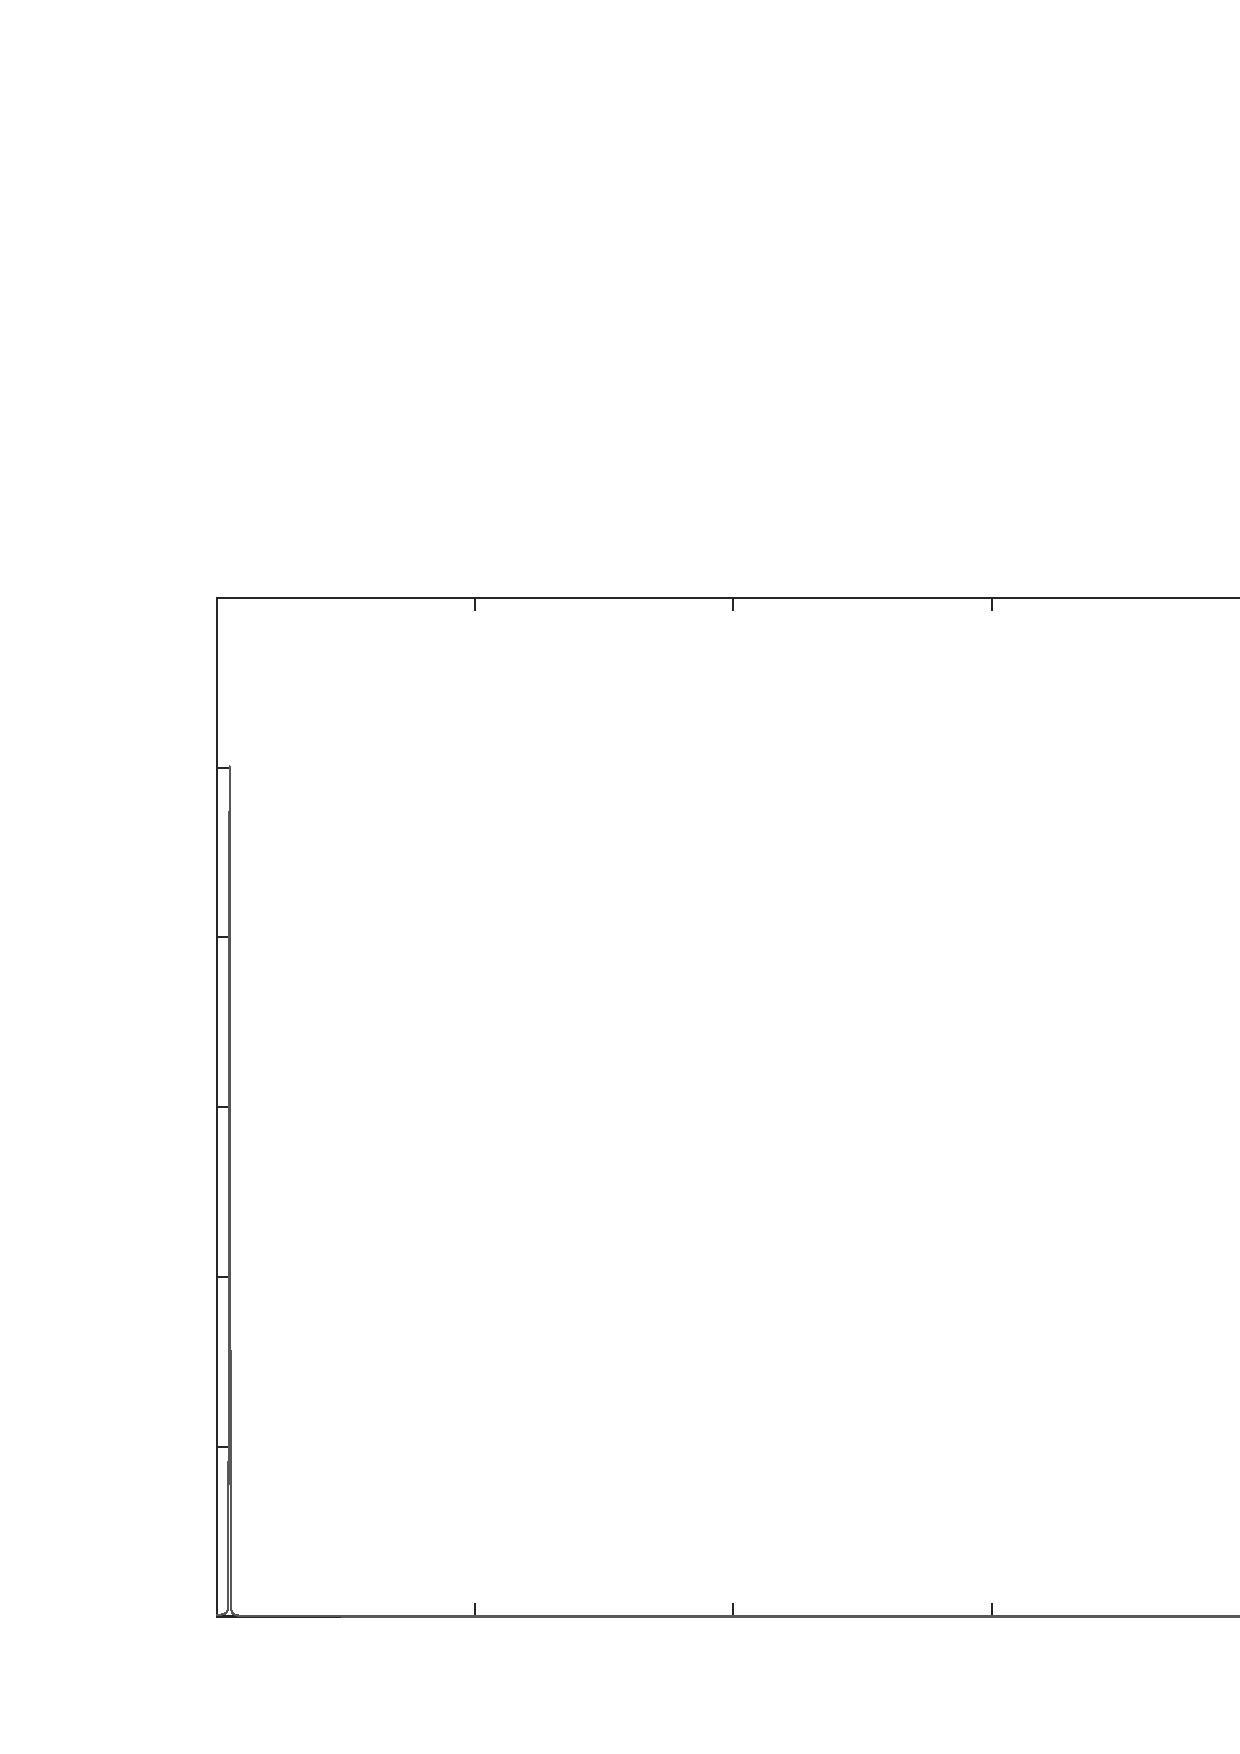
\includegraphics[scale=1]{octaves/cosineFT-inc}
\end{picture}%
\begin{picture}(800,600)(0,0)
\fontsize{13}{0}\selectfont\put(104,55.5788){\makebox(0,0)[t]{\textcolor[rgb]{0.15,0.15,0.15}{{0}}}}
\fontsize{13}{0}\selectfont\put(228,55.5788){\makebox(0,0)[t]{\textcolor[rgb]{0.15,0.15,0.15}{{0.2}}}}
\fontsize{13}{0}\selectfont\put(352,55.5788){\makebox(0,0)[t]{\textcolor[rgb]{0.15,0.15,0.15}{{0.4}}}}
\fontsize{13}{0}\selectfont\put(476,55.5788){\makebox(0,0)[t]{\textcolor[rgb]{0.15,0.15,0.15}{{0.6}}}}
\fontsize{13}{0}\selectfont\put(600,55.5788){\makebox(0,0)[t]{\textcolor[rgb]{0.15,0.15,0.15}{{0.8}}}}
\fontsize{13}{0}\selectfont\put(724,55.5788){\makebox(0,0)[t]{\textcolor[rgb]{0.15,0.15,0.15}{{1}}}}
\fontsize{13}{0}\selectfont\put(97.0525,66){\makebox(0,0)[r]{\textcolor[rgb]{0.15,0.15,0.15}{{0}}}}
\fontsize{13}{0}\selectfont\put(97.0525,147.5){\makebox(0,0)[r]{\textcolor[rgb]{0.15,0.15,0.15}{{100}}}}
\fontsize{13}{0}\selectfont\put(97.0525,229){\makebox(0,0)[r]{\textcolor[rgb]{0.15,0.15,0.15}{{200}}}}
\fontsize{13}{0}\selectfont\put(97.0525,310.5){\makebox(0,0)[r]{\textcolor[rgb]{0.15,0.15,0.15}{{300}}}}
\fontsize{13}{0}\selectfont\put(97.0525,392){\makebox(0,0)[r]{\textcolor[rgb]{0.15,0.15,0.15}{{400}}}}
\fontsize{13}{0}\selectfont\put(97.0525,473.5){\makebox(0,0)[r]{\textcolor[rgb]{0.15,0.15,0.15}{{500}}}}
\fontsize{13}{0}\selectfont\put(97.0525,555){\makebox(0,0)[r]{\textcolor[rgb]{0.15,0.15,0.15}{{600}}}}
\end{picture}

    }\caption{Plot of the Fourier Transform of \texttt{cos(2*pi*x)}. The two
    impulses are located very close to $0$ and $1$.}\label{oct:cosineFT}
\end{center}
\end{figure*}

\begin{figure*}[ht]
\begin{center}
\scalebox{0.5}{
% Title: gl2ps_renderer figure
% Creator: GL2PS 1.4.2, (C) 1999-2020 C. Geuzaine
% For: Octave
% CreationDate: Mon Oct 31 14:18:23 2022
\setlength{\unitlength}{1pt}
\begin{picture}(0,0)
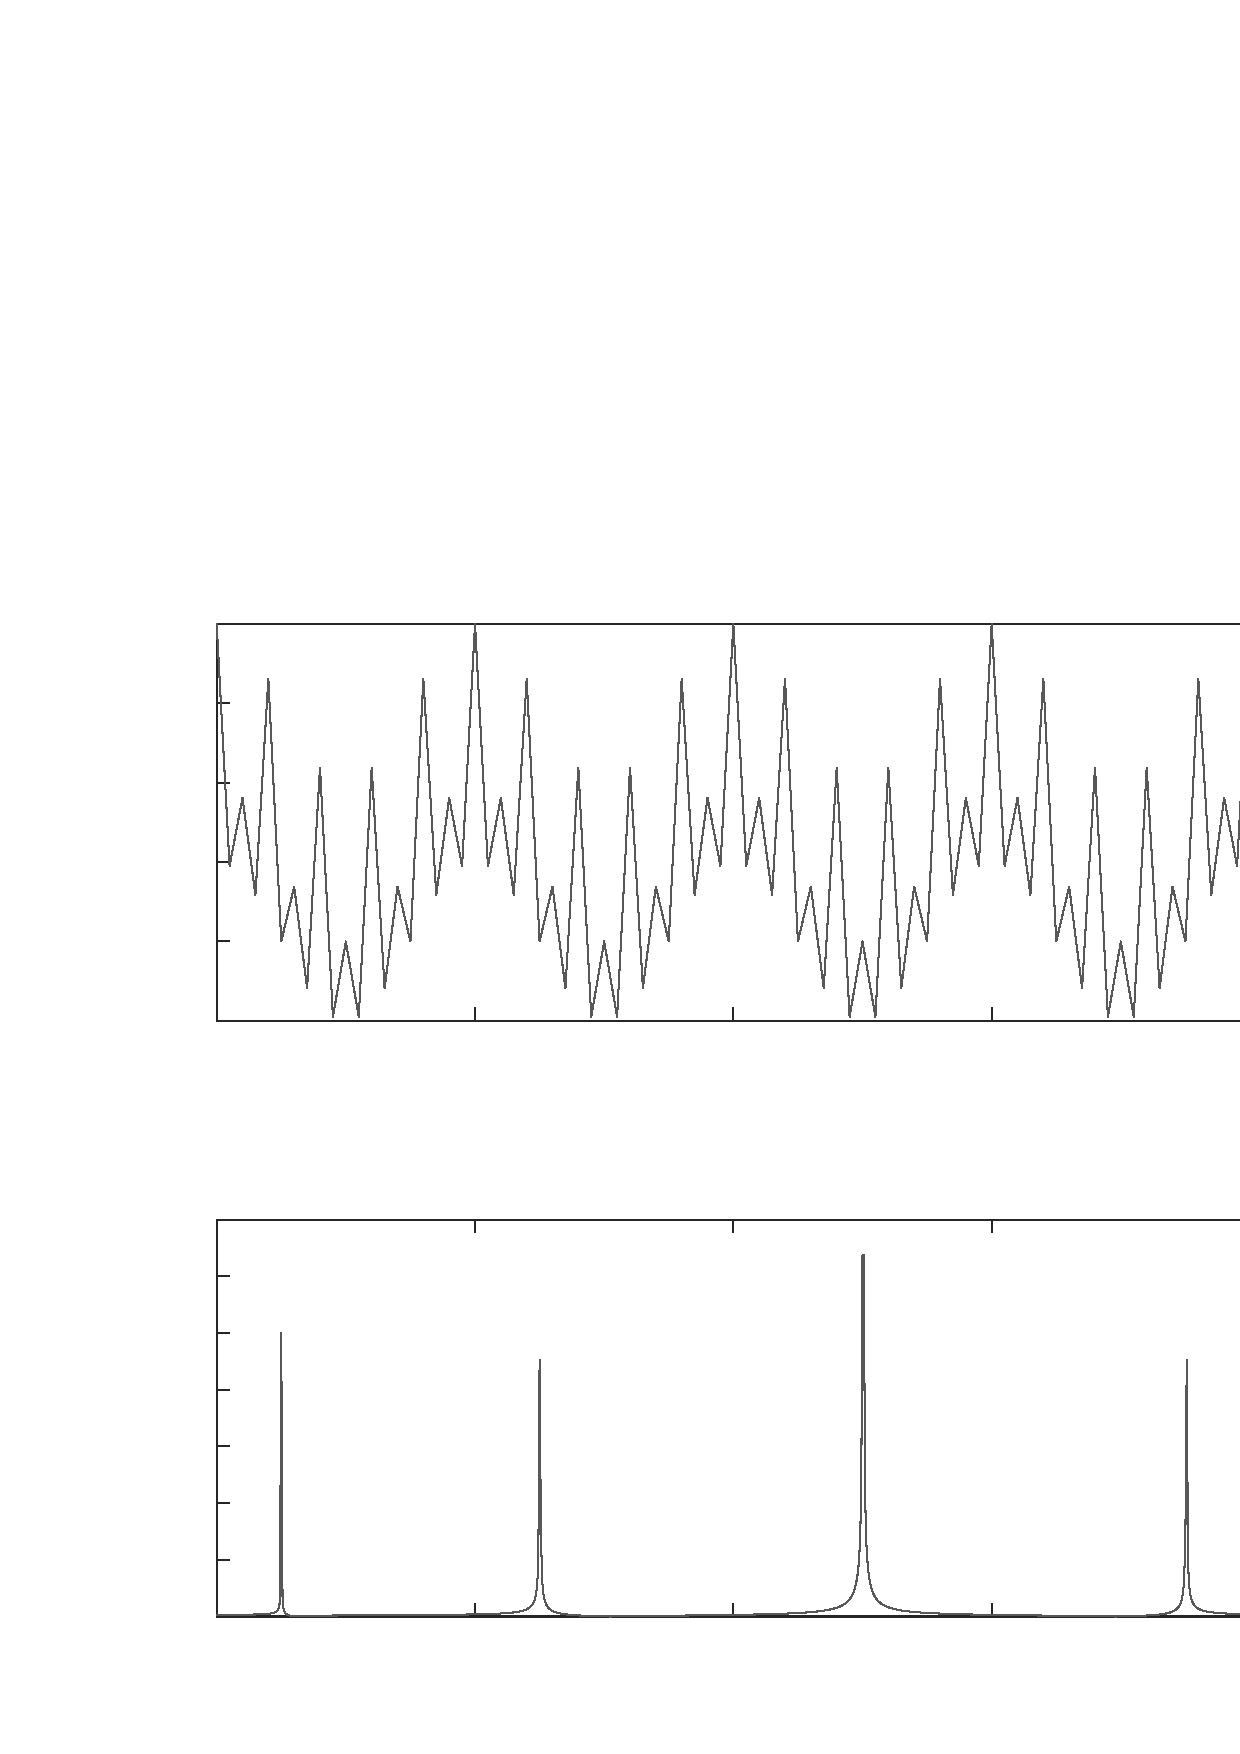
\includegraphics[scale=1]{octaves/cosineSumFT-inc}
\end{picture}%
\begin{picture}(800,600)(0,0)
\fontsize{13}{0}\selectfont\put(104,341.475){\makebox(0,0)[t]{\textcolor[rgb]{0.15,0.15,0.15}{{0}}}}
\fontsize{13}{0}\selectfont\put(228,341.475){\makebox(0,0)[t]{\textcolor[rgb]{0.15,0.15,0.15}{{0.2}}}}
\fontsize{13}{0}\selectfont\put(352,341.475){\makebox(0,0)[t]{\textcolor[rgb]{0.15,0.15,0.15}{{0.4}}}}
\fontsize{13}{0}\selectfont\put(476,341.475){\makebox(0,0)[t]{\textcolor[rgb]{0.15,0.15,0.15}{{0.6}}}}
\fontsize{13}{0}\selectfont\put(600,341.475){\makebox(0,0)[t]{\textcolor[rgb]{0.15,0.15,0.15}{{0.8}}}}
\fontsize{13}{0}\selectfont\put(724,341.475){\makebox(0,0)[t]{\textcolor[rgb]{0.15,0.15,0.15}{{1}}}}
\fontsize{13}{0}\selectfont\put(97.0525,351.924){\makebox(0,0)[r]{\textcolor[rgb]{0.15,0.15,0.15}{{-2}}}}
\fontsize{13}{0}\selectfont\put(97.0525,390.024){\makebox(0,0)[r]{\textcolor[rgb]{0.15,0.15,0.15}{{-1}}}}
\fontsize{13}{0}\selectfont\put(97.0525,428.124){\makebox(0,0)[r]{\textcolor[rgb]{0.15,0.15,0.15}{{0}}}}
\fontsize{13}{0}\selectfont\put(97.0525,466.224){\makebox(0,0)[r]{\textcolor[rgb]{0.15,0.15,0.15}{{1}}}}
\fontsize{13}{0}\selectfont\put(97.0525,504.324){\makebox(0,0)[r]{\textcolor[rgb]{0.15,0.15,0.15}{{2}}}}
\fontsize{13}{0}\selectfont\put(97.0525,542.424){\makebox(0,0)[r]{\textcolor[rgb]{0.15,0.15,0.15}{{3}}}}
\fontsize{15}{0}\selectfont\put(414,552.424){\makebox(0,0)[b]{\textcolor[rgb]{0,0,0}{{Sum of cosines}}}}
\fontsize{13}{0}\selectfont\put(104,55.5514){\makebox(0,0)[t]{\textcolor[rgb]{0.15,0.15,0.15}{{0}}}}
\fontsize{13}{0}\selectfont\put(228,55.5514){\makebox(0,0)[t]{\textcolor[rgb]{0.15,0.15,0.15}{{0.2}}}}
\fontsize{13}{0}\selectfont\put(352,55.5514){\makebox(0,0)[t]{\textcolor[rgb]{0.15,0.15,0.15}{{0.4}}}}
\fontsize{13}{0}\selectfont\put(476,55.5514){\makebox(0,0)[t]{\textcolor[rgb]{0.15,0.15,0.15}{{0.6}}}}
\fontsize{13}{0}\selectfont\put(600,55.5514){\makebox(0,0)[t]{\textcolor[rgb]{0.15,0.15,0.15}{{0.8}}}}
\fontsize{13}{0}\selectfont\put(724,55.5514){\makebox(0,0)[t]{\textcolor[rgb]{0.15,0.15,0.15}{{1}}}}
\fontsize{13}{0}\selectfont\put(97.0525,66){\makebox(0,0)[r]{\textcolor[rgb]{0.15,0.15,0.15}{{0}}}}
\fontsize{13}{0}\selectfont\put(97.0525,93.2143){\makebox(0,0)[r]{\textcolor[rgb]{0.15,0.15,0.15}{{100}}}}
\fontsize{13}{0}\selectfont\put(97.0525,120.429){\makebox(0,0)[r]{\textcolor[rgb]{0.15,0.15,0.15}{{200}}}}
\fontsize{13}{0}\selectfont\put(97.0525,147.643){\makebox(0,0)[r]{\textcolor[rgb]{0.15,0.15,0.15}{{300}}}}
\fontsize{13}{0}\selectfont\put(97.0525,174.857){\makebox(0,0)[r]{\textcolor[rgb]{0.15,0.15,0.15}{{400}}}}
\fontsize{13}{0}\selectfont\put(97.0525,202.071){\makebox(0,0)[r]{\textcolor[rgb]{0.15,0.15,0.15}{{500}}}}
\fontsize{13}{0}\selectfont\put(97.0525,229.286){\makebox(0,0)[r]{\textcolor[rgb]{0.15,0.15,0.15}{{600}}}}
\fontsize{13}{0}\selectfont\put(97.0525,256.5){\makebox(0,0)[r]{\textcolor[rgb]{0.15,0.15,0.15}{{700}}}}
\fontsize{15}{0}\selectfont\put(414,266.5){\makebox(0,0)[b]{\textcolor[rgb]{0,0,0}{{Fourier Transform}}}}
\end{picture}

    }\caption{Signal $c(x) = \cos{2\pi 5 x} + \cos{2\pi 25 x} + \cos{2\pi 50x}$
    and its Fourier Transform. The resulting Fourier Transform, obtained with
    function \texttt{fft()}, is the superposition of three distinct
    frequencies, each related to one of the three sinusoids forming signal
    $c(x)$.}\label{oct:cosineSumFT}
\end{center}
\end{figure*}

Classic Fourier Transforms suffer from crucial limitations. Undeniably, due to the uncertainty principle they cannot provide \emph{simultaneous} time and frequency localization. This means that, for instance, delta impulses in the frequency domain are likely generated by very long, if not infinite, sinusoids in the time domain---vice versa, brief signals in the time domain will yield a Fourier Transform with a very large band. In addition, they are not exactly useful for analyzing \emph{time-variant, non-stationary} signals\footnote{ Time-variant, non-stationary signals are the class of signals whose spectrum changes overtime.}, as the frequency of such signals or sequences is subject to possible variations whilst the content of the signal alters across time, resulting in a confusing frequency description.

Typically, noise in Fourier Transform is caused by abrupt changes in frequency of the signal---the more sudden the change in the speed of oscillation of the signal, the greater the noise will be produced. The result frequency description is still an faithful portrait of the signal's frequency content; still, added noise and multiple frequencies due to the non-stationary nature of the considered signal will yield a chaotic Fourier Transform which is hard to interpret.

The answer to this issue is the \textbf{Short Time Fourier Transform}, abbreviated in STFT. The key concept behind the short time Fourier Transform is to appropriately segment the time-variant signal into narrow time intervals, thin enough that the portion of the signal in it can be considered stationary. For each segment, perform a Fourier Transform of it: each Fourier Transform will provide the spectral information of a separate segment of the signal, yielding \emph{simultaneous} time and frequency information.

This means that the STFT involves computing the frequency description of the
time-domain segment \emph{and} keeping the information on which segment has
been transformed. In other words, the steps can be summarized as:
\begin{enumerate}
    \item choose a window function $W(t)$ of finite length, in order to select a
        narrow portion of the original signal;
    \item start with the window at position $t = 0$;
    \item truncate the signal with the window to obtain a segment of the
        original signal;
    \item compute the Fourier Transform of the segment, conveniently store the
        result;
    \item incrementally slide the window of $t'$ to the right, as needed, hence
        obtain $W(t - t')$;
    \item go to step $3$ until the window has covered the entire signal;
\end{enumerate}

Operating such procedure will yield results that can be collected in a data
structure; each Fourier Transform can be mathematically described in the following manner,
\begin{equation}\label{eqn:shortTimeFourierTransform}
    \mathrm{STFT}^u_f(t', u) = \int_t \left[f(t) \cdot W(t - t')\right]e^{-j2\pi ut}dt,
\end{equation}
where $t'$ is the \emph{time parameter} that controls the amount of shifting the window is subject to, $u$ is the frequency parameter, $f$ is the original signal $f(t)$, $W(t)$ is the windowing function, centered at $t = t'$. In brief, the operation involved is the transform of the signal $f(t)W(t - t')$ with the frequency variable $u$.

The windowing function is free to choose as desired. The shape of it could be rectangular, Gaussian, triangular, and so on. The window should be narrow enough to ensure that the portion of the signal falling withing the window \emph{is stationary}, but at the same time very narrow windows offer \emph{poor localization} in the frequency domain. This is because the Short Time Fourier Transform, as with any other Fourier Transform, is heavily dependent on the uncertainty principle---as such, there is a trade--off between \emph{localization in the frequency domain} and \emph{localization in the time domain}.

A choice of $W(t)\equiv 1$ would yield an infinitely long window: the STFT turns into a simple FT, providing exemplary frequency localization but nonexistent time localization. On contrary, a choice of $W(t) = \delta(t)$ would yield an infinitesimally short window, resulting in the time signal itself\footnote{In fact, 
\[
    \mathrm{STFT}^u_f(t', u) = \int_t \left[f(t) \cdot \delta(t - t')\right]e^{-j2\pi ut}dt = f(t')e^{-jut'},
\] with a single $f(t')$ transformed.}---but with a phase factor added---providing maximal time localization, but vacant frequency localization. Anything in between will yield a compromise between the two extremes, with wide windows assuring good frequency and poor time resolution, and narrow windows providing good time resolution at the expense of the frequency resolution.

It is clear that, especially in the case of signals whose content changes \emph{a lot} during time, a single window choice cannot possibly fit the entire signal and describe it efficiently. A way to overcome this limitation is to use the \textbf{wavelets}. Wavelets technique makes use of \emph{multiple window sizes} in order to catch various facets of the signal to analyze, capable of adjusting to the time-varying frequency. In order to localize frequency, a decent amount of signal should be processed---but the larger the span, the fewer the time localization.

The \textbf{uncertainty principle} was mathematically coded by scientist \emph{Werner Heisenberg} in 1927, and is any of a variety of mathematical inequalities asserting a fundamental limit to the accuracy with which the values for certain pairs of physical quantities of a particle, such as position, $x$, and momentum, $p$, can be predicted from initial conditions\cite{bib:wernerHeisemberg}.

Such variable pairs are known as complementary variables or canonically conjugate variables; and, depending on interpretation, the uncertainty principle limits to what extent such conjugate properties maintain their approximate meaning, as the mathematical framework of quantum physics does not support the notion of simultaneously well-defined conjugate properties expressed by a single value. The uncertainty principle implies that it is in general not possible to predict the value of a quantity with arbitrary certainty, even if all initial conditions are specified\cite{bib:wernerHeisemberg}.

Related to digital signal processing, the uncertainty principle gathers in the
form of
\begin{equation}\label{eqn:uncertaintyPrinciple}
    \Delta t \cdot \Delta f \geq \frac 1 {4\pi},
\end{equation}
where $\Delta t$ is the \emph{time resolution}---how well two spikes in time can be separated from each other in the frequency domain---and $\Delta f$ is the \emph{frequency resolution}---how well two spectral components can be divided from each other in the time domain. The unquestionable fact is that \emph{both $\Delta t$ and $\Delta f$ cannot be made arbitrarily small}: shrinking one of the two will incontrovertibly grow the other, and vice versa!

This fundamental law of nature can never be infringed, signifying that one cannot know the \emph{exact} time-frequency representation of a signal, since it must abide to the uncertainty principle and will be subject to a trade--off between time resolution and frequency resolution: one can only know what inverval of frequencies belongs to a given time interval. Wavelets are windows whose value take in account the product $\Delta t \Delta f$, and can be represented by rectangles having base $\Delta f$ and height $\Delta t$. The area of the wavelets cannot go below the value $\Delta t \cdot \Delta f$.

\section{Discrete Cosine Transform}\label{sec:discreteCosineTransform}

In Section~\ref{sec:basisFunctions} we explored the definition and some properties of basis functions regarding orthogonal transforms. The last ones were useful in particular, since they allow to exploit their energy compaction property, efficiently representing the transformed sequence with less coefficients than otherwise required.

Now, it is about time to introduce new transforms: let's begin with the \textbf{Discrete Cosine Transform (DFT)}, a transform with good compaction properties, generally exhibiting satisfactory performance for signals having strong autocorrelation.

\begin{defin}[Discrete Cosine Transform]
    Let $x[n]$ be a sequence with (possibly) strong autocorrelation. Then, its \emph{Discrete Cosine Transform (DCT)} is
    \begin{equation}\label{eqn:discreteCosineTransform}
        X[k] = \alpha(k) \sum_{n=0}^{N-1} x[n] \cos{\left(\frac{\pi(2n + 1)k}{2N}\right)};
    \end{equation}
    with $\alpha(0) = \sqrt{\frac 1 N}$ and $\alpha(k) = \sqrt{ \frac 2 N }$. Its \emph{inverse transform} is given by
    \begin{equation}\label{eqn:discreteCosineTransformInverse}
        x[n] = \sum_{k=0}^{N-1}\alpha(k)  X[k] \cos{\left(\frac{\pi(2n + 1)k}{2N}\right)},
    \end{equation}
    resulting from the choice of \emph{basis functions} \[\psi^*(n, k) = \cos{\left(\frac{\pi(2n + 1)k}{2N}\right)}\] and \[\psi(n, k) = \cos{\left(\frac{\pi(2n + 1)k}{2N}\right)}.\]
    In matrix form, one has
    \begin{equation}\label{eqn:discreteCosineTransformMatrixForm}
        \begin{array}{cc}
            \bm X = \bm{Cx} & \bm x = \bm C^{*\top} \bm X = \bm C^\top \bm X.
        \end{array}
    \end{equation}
\end{defin}

To begin with, consider that in this case $\psi^*(n, k) = \psi(n, k)$ as $\cos^*{(x)} = \cos{(x)}$ for any argument. Furthermore, the Discrete Cosine Transform of a real sequence \emph{is real}, as no complex unit is involved in its computation. Third, unlike the DFT, the Discrete Cosine Transform is \emph{not} symmetrical around $\pi$.

A discrete cosine transform (DCT) expresses a finite sequence of data points in terms of a sum of cosine functions oscillating at different frequencies. The DCT, first proposed by Nasir Ahmed in 1972, is a widely used transformation technique in signal processing and data compression. It is used in most digital media, including digital images (such as JPEG and HEIF, where small high-frequency components can be discarded), digital video (such as MPEG and H.26x), digital audio (such as Dolby Digital, MP3 and AAC), digital television (such as SDTV, HDTV and VOD), digital radio (such as AAC+ and DAB+), and speech coding (such as AAC-LD, Siren and Opus). DCTs are also important to numerous other applications in science and engineering, such as digital signal processing, telecommunication devices, reducing network bandwidth usage, and spectral methods for the numerical solution of partial differential equations.

The use of cosine rather than sine functions is critical for compression, since it turns out (as described below) that fewer cosine functions are needed to approximate a typical signal, whereas for differential equations the cosines express a particular choice of boundary conditions. In particular, a DCT is a Fourier-related transform similar to the discrete Fourier transform (DFT), but using only real numbers. The DCTs are generally related to Fourier Series coefficients of a periodically and symmetrically extended sequence whereas DFTs are related to Fourier Series coefficients of only periodically extended sequences. DCTs are equivalent to DFTs of roughly twice the length, operating on real data with even symmetry (since the Fourier transform of a real and even function is real and even), whereas in some variants the input and/or output data are shifted by half a sample. There are eight standard DCT variants, of which four are common\cite{bib:discreteCosineTransform}.

The Discrete Cosine Transform can be related to the Discrete Fourier Transform. Let us defined the \emph{half-sample, symmetric, right periodic extension} of $x$ as
\[
    x_s[n] =
    \left\{
        \begin{array}{ll}
            x[n] & 0 \leq n \leq N-1\\
            x[2N - 1 - n] & N \leq n \leq 2N-1
        \end{array}
    \right.
\]
that yields a sequence of the form
\begin{align*}
    x_s[n] = \{ &\dots, x[0], x[1],\dots,x[N-2], x[N-1],\\ 
                &x[N-1], x[N-2],\dots,x[1],x[0],\dots\}.
\end{align*}
According to the type of chosen periodic extension, up to $8$ different versions of the DCT can be obtained. The DFT of $x_s$ will thus be
\begin{align*}
    X_s[k] 
    &= \sum_{n=0}^{2N-1} x_s[n] e^{-j\frac{2\pi}{2N}kn}\\
    &= \sum_{n=0}^{N-1} x[n] e^{-j\frac{2\pi}{2N}kn} + \sum_{n=N}^{2N-1} x[2N - 1 - n] e^{-j\frac{2\pi}{2N}kn},
\end{align*}
and by substituting $m = 2N-1-n$ one soon obtains that
\begin{align*}
    n &= N  \rightarrow  m = N - 1 \\
    n &= 2N - 1  \rightarrow  m = 0 \\
    m &= 2N - 1 - n\\
    n &= 2N - 1 - m.
\end{align*}
Ultimately, the DCT will be
\begin{align*}
    X_s[k] 
    &= \sum_{n=0}^{N-1} x[n] e^{-j\frac{2\pi}{2N}kn} + \sum_{n=N}^{2N-1} x[\underbrace{2N - 1 - n}_{m}] e^{-j\frac{2\pi}{2N}kn}\\
    &= \sum_{n=0}^{N-1} x[n] e^{-j\frac{2\pi}{2N}kn} + \sum_{m=0}^{N-1} x[m] e^{-j\frac{2\pi}{2N}k(2N-1-m)}\\
    &= \sum_{n=0}^{N-1} x[n] e^{-j\frac{2\pi}{2N}kn} + \sum_{n=0}^{N-1} x[n] e^{-j\frac{2\pi}{2N}k(-1-n)}\\
    &= \sum_{n=0}^{N-1} x[n]\left(e^{-j\frac{2\pi}{2N}kn} + e^{-j\frac{2\pi}{2N}k(-1-n)}\right) \\
    &= \sum_{n=0}^{N-1} x[n]\left(e^{-j\frac{2\pi}{2N}kn} + e^{-j\frac{2\pi}{2N}k(-1-n)}\right) \cdot e^{j\frac{2\pi}{2N}\frac{k}{2}} e^{-j\frac{2\pi}{2N}\frac{k}{2}}\\
    &= e^{j\frac{2\pi}{2N}\frac{k}{2}} \sum_{n=0}^{N-1} x[n]\left(e^{-j\frac{2\pi}{2N}k(n + \frac 1 2)} + e^{+j\frac{2\pi}{2N}k(n + \frac 1 2)}\right)\\
    &= 2e^{j\frac{2\pi}{2N}\frac{k}{2}} \sum_{n=0}^{N-1} x[n]\left(\cos{(\frac{2\pi}{2N}k(n + \frac 1 2))}\right),
\end{align*}
which is equal to the DCT of $\bm x$, apart from scaling factors. Thus, it is possible to calculate the Discrete Cosine Transform by means of the Fast Fourier Transform, by first producing two \emph{half-sample, symmetric, right periodic extensions} of $x$, then summing up the Discrete Fourier Transform of these two sequences to obtain the Discrete Cosine Transform.

The periodicity artifacts are smaller in the DCT than in the DFT. Let an input sequence be of the following type,
\begin{center}
    \begin{tikzpicture}
        \draw[thick,-stealth] (-1.5,0) -- (1.5,0) node[anchor=north west] {$n$};
        \draw[-{Circle[open]}] (-2*0.2,0) -- (-2*0.2,0.5);
        \draw[-{Circle[open]}] (-1*0.2,0) -- (-1*0.2,1.4*0.5);
        \draw[-{Circle[open]}] (0*0.2,0) -- (0*0.2,1.8*0.5);
        \draw[-{Circle[open]}] (1*0.2,0) -- (1*0.2,2.2*0.5);
        \draw[-{Circle[open]}] (2*0.2,0) -- (2*0.2,2.6*0.5);
    \end{tikzpicture}
\end{center}
the periodicity artifacts induced by the periodic extensions are sudden jumps located ad the ``discontinuity'' on a new repetition:
\begin{center}
    \begin{tikzpicture}
        \draw[thick,-stealth] (-2.5,0) -- (2.5,0) node[anchor=north west] {$n$};
        \draw[-{Circle[open]}] (-1+-2*0.2,0) -- (-1+-2*0.2,0.5);
        \draw[-{Circle[open]}] (-1+-1*0.2,0) -- (-1+-1*0.2,1.4*0.5);
        \draw[-{Circle[open]}] (-1+0*0.2,0) --  (-1+0*0.2,1.8*0.5);
        \draw[-{Circle[open]}] (-1+1*0.2,0) --  (-1+1*0.2,2.2*0.5);
        \draw[-{Circle[open]}] (-1+2*0.2,0) --  (-1+2*0.2,2.6*0.5);
        \draw[-{Circle[open]}] (-2*0.2,0) -- (-2*0.2,0.5);
        \draw[-{Circle[open]}] (-1*0.2,0) -- (-1*0.2,1.4*0.5);
        \draw[-{Circle[open]}] (0*0.2,0) -- (0*0.2,1.8*0.5);
        \draw[-{Circle[open]}] (1*0.2,0) -- (1*0.2,2.2*0.5);
        \draw[-{Circle[open]}] (2*0.2,0) -- (2*0.2,2.6*0.5);
        \draw[-{Circle[open]}] (+1+-2*0.2,0) -- (+1+-2*0.2,0.5);
        \draw[-{Circle[open]}] (+1+-1*0.2,0) -- (+1+-1*0.2,1.4*0.5);
        \draw[-{Circle[open]}] (+1+0*0.2,0) --  (+1+0*0.2,1.8*0.5);
        \draw[-{Circle[open]}] (+1+1*0.2,0) --  (+1+1*0.2,2.2*0.5);
        \draw[-{Circle[open]}] (+1+2*0.2,0) --  (+1+2*0.2,2.6*0.5);
        \node[] at (-1.8, .55) {$\cdots$};
        \node[] at (+1.8, .55) {$\cdots$};
    \end{tikzpicture}
\end{center}

Now, confront this with the pattern induced by the Discrete Cosine Transform, which involves ``mirroring'' the sequence as well as periodicizing it:
\begin{center}
    \begin{tikzpicture}
        \draw[thick,-stealth] (-2.5,0) -- (3.5,0) node[anchor=north west] {$n$};
        \draw[-{Circle[open]}] (-1+2*0.2,0) -- (-1+2*0.2,0.5);
        \draw[-{Circle[open]}] (-1+1*0.2,0) -- (-1+1*0.2,1.4*0.5);
        \draw[-{Circle[open]}] (-1+0*0.2,0) --  (-1+0*0.2,1.8*0.5);
        \draw[-{Circle[open]}] (-1+-1*0.2,0) --  (-1+-1*0.2,2.2*0.5);
        \draw[-{Circle[open]}] (-1+-2*0.2,0) --  (-1+-2*0.2,2.6*0.5);
        \draw[-{Circle[open]}] (-2*0.2,0) -- (-2*0.2,0.5);
        \draw[-{Circle[open]}] (-1*0.2,0) -- (-1*0.2,1.4*0.5);
        \draw[-{Circle[open]}] (0*0.2,0) -- (0*0.2,1.8*0.5);
        \draw[-{Circle[open]}] (1*0.2,0) -- (1*0.2,2.2*0.5);
        \draw[-{Circle[open]}] (2*0.2,0) -- (2*0.2,2.6*0.5);
        \draw[-{Circle[open]}] (2+-1+2*0.2,0) --   (2+-1+2*0.2,0.5);
        \draw[-{Circle[open]}] (2+-1+1*0.2,0) --   (2+-1+1*0.2,1.4*0.5);
        \draw[-{Circle[open]}] (2+-1+0*0.2,0) --   (2+-1+0*0.2,1.8*0.5);
        \draw[-{Circle[open]}] (2+-1+-1*0.2,0) --  (2+-1+-1*0.2,2.2*0.5);
        \draw[-{Circle[open]}] (2+-1+-2*0.2,0) --  (2+-1+-2*0.2,2.6*0.5);
        \draw[-{Circle[open]}] (2+-2*0.2,0) --     (2+-2*0.2,0.5);
        \draw[-{Circle[open]}] (2+-1*0.2,0) --     (2+-1*0.2,1.4*0.5);
        \draw[-{Circle[open]}] (2+0*0.2,0) --      (2+0*0.2,1.8*0.5);
        \draw[-{Circle[open]}] (2+1*0.2,0) --      (2+1*0.2,2.2*0.5);
        \draw[-{Circle[open]}] (2+2*0.2,0) --      (2+2*0.2,2.6*0.5);
        \node[] at (-1.8, .55) {$\cdots$};
        \node[] at (+2.8, .55) {$\cdots$};
    \end{tikzpicture}
\end{center}
so that no sudden jumps or whatsoever occur. The Discrete Cosine Transform ``mirrors'' the sequence when periodicizing it, doubling the period and modifying it slightly, but making less room for periodicity artifacts. Discrete Cosine Transforms are employed in \texttt{mp3} coding (MCDT) and in \texttt{JPEG} coding (2--D DCT).

\section{Walsh--Hadamard Transform}\label{sec:walshHadamardTransform}

Another extremely simple and \emph{real} orthogonal transform is the \textbf{Walsh--Hadamard Transform}. The Walsh--Hadamard transform has the following form,
\begin{equation}\label{eqn:walshHadamardTransform}
    \left\{
        \begin{array}{lll}
            X[0] & = & \frac{x[0] + x[1]}{\sqrt 2}\\
            X[1] & = & \frac{x[0] - x[1]}{\sqrt 2}\\
        \end{array}
    \right.
\end{equation}
with its \emph{inverse transform}
\begin{equation}\label{eqn:walshHadamardTransformInverse}
    \left\{
        \begin{array}{lll}
            x[0] & = & \frac{X[0] + X[1]}{\sqrt 2}\\
            x[1] & = & \frac{X[0] - X[1]}{\sqrt 2}\\
        \end{array}
    \right..
\end{equation}
The factor $\sqrt 2$ at the denominator is indeed a scaling factor, and at convenience it can be applied squared in either the direct or the inverse form. The matrix form is as follows
\begin{equation}\label{eqn:walshHadamardTransformMatrixForm}
    \bm F = \frac {1}{\sqrt 2}\begin{Vmatrix} 1 & 1 \\ 1 & -1 \end{Vmatrix}, \bm F_{inv} = \frac{1}{\sqrt 2}\begin{Vmatrix} 1 & 1 \\ 1 & -1 \end{Vmatrix} = \bm F^{-1} = \bm F^\top \equiv \bm F,
\end{equation}
with its inverse equal to the direct form.

A generalization of the Walsh--Hadamard Transforms makes use of \emph{higher-order matrices}, for which a parameter $N$ is the number of columns and rows of the matrix form $\bm H$. In the case $N=2$, one obtains \[\bm H_1 = \bm F = \frac{1}{\sqrt{2}}\begin{bmatrix} 1 & 1 \\ 1 & -1 \end{bmatrix},\] hence for $N=2$ one has the Walsh--Hadamard transform.

Matrices for the higher-oder transforms can be derived using recursion in the following manner,
\[
    \bm H_2 = \bm H_1 \otimes \bm H_1 = \frac {1} {\sqrt 2}
    \begin{bmatrix}
    \bm H_1 & \bm H_1 \\
    \bm H_1 & - \bm H_1
    \end{bmatrix}
    = \frac {1} {\sqrt 4}
    \begin{bmatrix}
        1 & 1 & 1 & 1\\
        1 & -1 & 1 & -1\\
        1 & 1 & -1 & -1\\
        1 & -1 & -1 & 1
    \end{bmatrix}
\]

\begin{align*}
    \bm H_3 &= \bm H_2 \otimes \bm H_2 = \frac {1} {\sqrt 2}
    \begin{bmatrix}
    \bm H_2 & \bm H_2 \\
    \bm H_2 & - \bm H_2
    \end{bmatrix}\\
    &= \frac {1} {\sqrt 8}
    \begin{bmatrix}
        1 & 1 & 1 & 1 & 1 & 1 & 1 & 1\\
        1 & -1 & 1 & -1 & 1 & -1 & 1 & -1 \\
        1 & 1 & -1 & -1 & 1 & 1 & -1 & -1 \\
        1 & -1 & -1 & 1 & 1 & -1 & -1 & 1 \\
        1 & 1 & 1 & 1 & -1 & -1 & -1 & -1 \\
        1 & -1 & 1 & -1 & -1 & 1 & -1 & 1 \\
        1 & 1 & -1 & -1 & -1 & -1 & 1 & 1 \\
        1 & -1 & -1 & 1 & -1 & 1 & 1 & -1
    \end{bmatrix}
\end{align*}
Any matrix $\bm H$ is real, symmetric and orthogonal; accordingly, one has
\[
    \bm H = \bm H^* = \bm H^\top = \bm H^{-1}
\]
with the forward and inverse transforms
\begin{align*}
    \bm X &= \bm {Hx}\\
    \bm x &= \bm {HX}
\end{align*}
that are identical.

\begin{figure*}[ht]
    \begin{center}
        \begin{tikzpicture}
            \draw (-4,0) -- (4,0) node[anchor=north west] {};
            \draw (-4,-1) -- (4,-1) node[anchor=north west] {};
            \draw (-4,-2) -- (4,-2) node[anchor=north west] {};
            \draw (-4,-3) -- (4,-3) node[anchor=north west] {};
            \draw (-4,-4) -- (4,-4) node[anchor=north west] {};
            \draw (-4,-5) -- (4,-5) node[anchor=north west] {};
            \draw (-4,-6) -- (4,-6) node[anchor=north west] {};
            \draw (-4,-7) -- (4,-7) node[anchor=north west] {};

            \node at (-5, 1) {Hadamard ordering};
            \node at (+5, 1) {Walsh ordering};
            \node at (-5, 0) {$0$};
            \node at (+5, 0) {$0$};
            \draw[thick, blue] (-4, 0) -- (-4, 0.3) -- (4, 0.3) -- (4, 0);
            \node at (-5, -1) {$1$};
            \node at (+5, -1) {$7$};
            \draw[thick, blue]
                (-4, -1) --
                (-4, -1+0.3) --
                (-3, -1+0.3) --
                (-3, -1-0.3) --
                (-2, -1-0.3) --
                (-2, -1+0.3) --
                (-1, -1+0.3) --
                (-1, -1-0.3) --
                (0, -1-0.3) --
                (0, -1+0.3) --
                (1, -1+0.3) --
                (1, -1-0.3) --
                (2, -1-0.3) --
                (2, -1+0.3) --
                (3, -1+0.3) --
                (3, -1-0.3) --
                (4, -1-0.3) --
                (4, -1);
            \node at (-5, -2) {$2$};
            \node at (+5, -2) {$3$};
            \draw[thick, blue]
                (-4, -2) --
                (-4, -2+0.3) --
                (-2, -2+0.3) --
                (-2, -2-0.3) --
                (0, -2-0.3) --
                (0, -2+0.3) --
                (2, -2+0.3) --
                (2, -2-0.3) --
                (4, -2-0.3) --
                (4, -2);
            \node at (-5, -3) {$3$};
            \node at (+5, -3) {$4$};
            \draw[thick, blue]
                (-4, -3) --
                (-4, -3+0.3) --
                (-3, -3+0.3) --
                (-3, -3-0.3) --
                (-1, -3-0.3) --
                (-1, -3+0.3) --
                (1, -3+0.3) --
                (1, -3-0.3) --
                (3, -3-0.3) --
                (3, -3+0.3) --
                (4, -3+0.3) --
                (4, -3);
            \node at (-5, -4) {$4$};
            \node at (+5, -4) {$1$};
            \draw[thick, blue]
                (-4, -4) --
                (-4, -4+0.3) --
                (0, -4+0.3) --
                (0, -4-0.3) --
                (4, -4-0.3) --
                (4, -4);
            \node at (-5, -5) {$5$};
            \node at (+5, -5) {$6$};
            \draw[thick, blue]
                (-4, -5) --
                (-4, -5+0.3) --
                (-3, -5+0.3) --
                (-3, -5-0.3) --
                (-2, -5-0.3) --
                (-2, -5+0.3) --
                (-1, -5+0.3) --
                (-1, -5-0.3) --
                (1, -5-0.3) --
                (1, -5+0.3) --
                (2, -5+0.3) --
                (2, -5-0.3) --
                (3, -5-0.3) --
                (3, -5+0.3) --
                (4, -5+0.3) --
                (4, -5);
            \node at (-5, -6) {$6$};
            \node at (+5, -6) {$2$};
            \draw[thick, blue]
                (-4, -6) --
                (-4, -6+0.3) --
                (-2, -6+0.3) --
                (-2, -6-0.3) --
                (2, -6-0.3) --
                (2, -6+0.3) --
                (4, -6+0.3) --
                (4, -6);
            \node at (-5, -7) {$7$};
            \node at (+5, -7) {$5$};
            \draw[thick, blue]
                (-4, -7) --
                (-4, -7+0.3) --
                (-3, -7+0.3) --
                (-3, -7-0.3) --
                (-1, -7-0.3) --
                (-1, -7+0.3) --
                (0, -7+0.3) --
                (0, -7-0.3) --
                (1, -7-0.3) --
                (1, -7+0.3) --
                (3, -7+0.3) --
                (3, -7-0.3) --
                (4, -7-0.3) --
                (4, -7);
        \end{tikzpicture}
    \end{center}\caption{Wavelets corresponding to Walsh--Hadamard transforms orders. Ordering is denoted on the side.}\label{tikz:walshHadamardTransformWavelets}
\end{figure*}

\section{Haar Transform}\label{sec:haarTransform}

A different recursion definition leads to \textbf{Haar Transforms}. For instance, for $N=8$ one obtains
\begin{equation}\label{eqn:haarTransformExample}
    \bm H_8 = \frac {1}{\sqrt 8}
    \begin{bmatrix}
        1 & 1 & 1 & 1 & 1 & 1 & 1 & 1\\
        1 & 1 & 1 & 1 & -1 & -1 & -1 & -1\\
        \sqrt 2 & \sqrt 2 & \sqrt 2 & \sqrt 2 & 0 & 0 & 0 & 0\\
        0 & 0 & 0 & 0 & \sqrt 2 & \sqrt 2 & \sqrt 2 & \sqrt 2\\
        2 & -2 & 0 & 0 & 0 & 0 & 0 & 0\\
        0 & 0 & 2 & -2 & 0 & 0 & 0 & 0\\
        0 & 0 & 0 & 0 & 2 & -2 & 0 & 0\\
        0 & 0 & 0 & 0 & 0 & 0 & 2 & -2\\
    \end{bmatrix}
    \begin{matrix}
        \varphi_0(t)\\
        \varphi_1(t)\\
        \psi_{1,0}(t)\\
        \psi_{1,1}(t)\\
        \psi_{2,0}(t)\\
        \psi_{2,1}(t)\\
        \psi_{2,2}(t)\\
        \psi_{2,3}(t)\\
    \end{matrix}
\end{equation}


Haar transforms are described by \emph{wavelets}, that are small squared pulses that can be shifted in location. ``Row'' functions describe those wavelets. Functions $\varphi_0(t)$ and $\varphi_1(t)$ are similar to the row of the Walsh--Hadamard matrix; lines described by functions $\psi_{i,j}(t)$ are instead different, with $i$ signifying the \emph{scale} with which the wavelet occurs---one starts from $1$ being of scale $\sqrt 2$ and then doubles as the order increases---and $j$ controlling the \emph{shift} of the wavelet described by that line. Those functions are said to be the \textbf{Haar functions}. Haar functions contain a single prototype shape: a square wave. The parameters specify the width--scale of the shape along with its shift. In this way one is able to represent not only the details in the signal, but also their locations in time.

Any transform that adopts wavelet is said to be a \emph{wavelet transform}; among them, the Haar is the simplest of all. Techniques such as \emph{Fast Haar Transform} have been designed\cite{bib:fastHaarTransform}.


\begin{figure*}[ht]
    \begin{center}
        \begin{tikzpicture}
            \draw[-stealth] (0,0) -- (2,0) node[anchor=north west] {};
            \draw[-stealth] (0,-1) -- (0,+1) node[anchor=north west] {};
            \draw[thick, blue] (0,.2) -- (1.8,.2);
        \end{tikzpicture}
        \begin{tikzpicture}
            \draw[-stealth] (0,0) -- (2,0) node[anchor=north west] {};
            \draw[-stealth] (0,-1) -- (0,+1) node[anchor=north west] {};
            \draw[thick, blue] (0,.2) -- (.9,.2) -- (+.9, -.2) -- (1.8,-.2);
        \end{tikzpicture}
        \begin{tikzpicture}
            \draw[-stealth] (0,0) -- (2,0) node[anchor=north west] {};
            \draw[-stealth] (0,-1) -- (0,+1) node[anchor=north west] {};
            \draw[thick, blue] (0,.2) -- (.45,.2) -- (+.45, -.2) -- (.9,-.2) -- (.9, 0);
        \end{tikzpicture}
        \begin{tikzpicture}
            \draw[-stealth] (0,0) -- (2,0) node[anchor=north west] {};
            \draw[-stealth] (0,-1) -- (0,+1) node[anchor=north west] {};
            \draw[thick, blue] (.9,0) -- (.9,.2) -- (.9+.45,.2) -- (.9++.45, -.2) -- (.9+.9,-.2) -- (.9+.9, 0);
        \end{tikzpicture}
        \\
        \begin{tikzpicture}
            \draw[-stealth] (0,0) -- (2,0) node[anchor=north west] {};
            \draw[-stealth] (0,-1) -- (0,+1) node[anchor=north west] {};
            \draw[thick, blue] (0,.2) -- (0+.225,.2) -- (0+.225, -.2) -- (0+.45,-.2) -- (.45, 0);
        \end{tikzpicture}
        \begin{tikzpicture}
            \draw[-stealth] (0,0) -- (2,0) node[anchor=north west] {};
            \draw[-stealth] (0,-1) -- (0,+1) node[anchor=north west] {};
            \draw[thick, blue] (.45, 0) -- (.45,.2) -- (.45+.225,.2) -- (.45+.225, -.2) -- (.45+.45,-.2) -- (.45+.45, 0);
        \end{tikzpicture}
        \begin{tikzpicture}
            \draw[-stealth] (0,0) -- (2,0) node[anchor=north west] {};
            \draw[-stealth] (0,-1) -- (0,+1) node[anchor=north west] {};
            \draw[thick, blue] (.9, 0) -- (.9,.2) -- (.9+.225,.2) -- (.9+.225, -.2) -- (.9+.45,-.2) -- (.9+.45, 0);
        \end{tikzpicture}
        \begin{tikzpicture}
            \draw[-stealth] (0,0) -- (2,0) node[anchor=north west] {};
            \draw[-stealth] (0,-1) -- (0,+1) node[anchor=north west] {};
            \draw[thick, blue] (1.35, 0) -- (1.35,.2) -- (1.35+.225,.2) -- (1.35+.225, -.2) -- (1.35+.45,-.2) -- (1.35+.45, 0);
        \end{tikzpicture}
    \end{center}\caption{Square wavelets associated with \emph{Haar Transform}. The parameters of the Haar transform specify the width and the location of the wavelet.}\label{tikz:haarTransformWavelets}
\end{figure*}

\chapter{$z$-Transform}\label{sec:zTransform}

In mathematics and signal processing, the $z$-Transform converts a discrete-time signal, which is a sequence of real or complex numbers, into a complex frequency-domain (z-domain or z-plane) representation.

It can be considered as a discrete-time equivalent of the Laplace transform (s-domain).

Whereas the continuous-time Fourier transform is evaluated on the Laplace s-domain's imaginary line, the discrete-time Fourier transform is evaluated over the unit circle of the z-domain. What is roughly the s-domain's left half-plane, is now the inside of the complex unit circle; what is the z-domain's outside of the unit circle, roughly corresponds to the right half-plane of the s-domain.

One of the means of designing digital filters is to take analog designs, subject them to a bilinear transform which maps them from the s-domain to the z-domain, and then produce the digital filter by inspection, manipulation, or numerical approximation. Such methods tend not to be accurate except in the vicinity of the complex unity, i.e. at low fre\-quen\-cies\cite{bib:zTransform}.

The Discrete-time Fourier Transform provides a frequency-domain representation of discrete-time signals and LTI dis\-cre\-te-time systems. Because of the convergence condition as in Equation~\ref{thm:existenceDTFT}, in many cases the DTFT of a sequence might not exist. As a consequence, it is not possible to make use of such frequency characterization in all cases where the transform does not converge.

A generalization of the Discrete-time Fourier Transform is the
\textbf{$z$-Transform}, defined by
\begin{equation}\label{eqn:zTransform}
    G(z) = \sum_{n=-\infty}^\infty g[n] z^{-n},
\end{equation}
where the \emph{$z$-frequency} $z := \Re{(z)} + j \Im{(z)}$ is a complex
variable.

If one lets $z = re^{j\omega}$, it is straightforward to notice that the
$z$-transform reduces to
\begin{equation}\label{eqn:zTransformInterpretation}
    G(re^{j\omega}) = \sum_{n=-\infty}^\infty g[n] r^{-n} e^{-j\omega n},
\end{equation}
and given that the formula for the Discrete-time Fourier Transform is
\[
    X(e^{j\omega}) = \sum_{n=-\infty}^\infty x[n]e^{-j\omega n}
\]
one concludes that $G(re^{j\omega})$ can be interpreted as the DTFT of the modified sequence $\{g[n]r^{-n}\}$. For $r = 1$ one has $|z| = 1$, and the $z$-transform reduces to its DTFT, provided the latter exists. For sure, the $z$-transform is decisive in all case where a DTFT of a sequence does not exist, hence when the sequece is not suitable to be transformed into Fourier domain.

Since a $z$-transform of a sequence $g[n]$ with $r = 1$ is completely equivalent to a DTFT of the same input sequence, the DTFT reduces to compute the $z$-transform and evaluating it at $z$-frequencies such that $|z| = 1$; this practically means that amid all possible complex frequencies, the DTFT is like evaluating the $z$-transform in the \textbf{unit circle} of radius $1$, that is the countour $|z| = 1$. The complex variable $z = re^{j\omega}$ can be split into two components, $r$ and a complex exponential $e^{j\omega}$. The first term is the \emph{distance between the point and the origin} in the z-plane (the radius), the second one determines the \emph{angle} at which the complex number is located. When $r=1$, we are basically lying in the contour of the unit circle as $z$ will possess module $|z|=1$. At last, the $z$-transform is an extension of the Discrete-time Fourier Transform, from the circle of radius $1$ to all complex domain.

\section{Properties of $z$-Transform}

\subsection{Region of Convergence}

Like the DTFT, there are conditions on the convergence of the infinite series in the definition~\ref{eqn:zTransform}; for a given sequence the set $\mathcal R$ of the values of $z$ among which the $z$-transform converges is said to be the \textbf{region of convergence (RoC)} of the $z$-transform.

In particular due to Theorem~\ref{thm:existenceDTFT}, the series
\[
    G(re^{j\omega}) = \sum_{n=-\infty}^\infty g[n] r^{-n} e^{-j\omega n}
\]
converges if the sequence $\{g[n]r^{-n}\}$ is absolutely summable, that is when
\[
    \sum_{n=-\infty}^\infty \left|g[n] r^{-n}\right| < \infty.
\]

The $z$-transform may converge only in a specific region of the z-plane, precisely the RoC. Let $r_-=\mathcal R_{g-}$ and $r_+ = \mathcal R_{g+}$ be the values of $r$ among which the $z$-transform converges; then, the sequence $g[n]r^{-n}$ is \emph{absolutely summable} for all such values of $r$, that is
\[
    \sum_{n=-\infty}^\infty \left|g[n] r^{-n}\right| < \infty
\]
in the range \[ 0 \leq r_- \leq r \leq r_+ \leq \infty.\] The annular region defined by the previous inequalities is called the \emph{region of convergence (RoC)} of $G(re^{j\omega}) = G(z)$, and can be geometrically illustrated as in the next Figure,

\begin{center}
    \begin{tikzpicture}
        \draw[thick,-stealth] (-2.5,0) -- (2.5,0) node[anchor=north west] {$\Re z$};
        \draw[thick,-stealth] (0,-2.5) -- (0,2.5) node[anchor=south east] {$\Im z$};
        \node[draw, circle, minimum size=4cm] at (0,0){};
        \node[draw, circle, minimum size=3cm] at (0,0){};
        \draw[-stealth] (0,0) -- (2*0.7071, 2*0.7071);
        \draw[-stealth] (0,0) -- (-1.5000*0.7071, 1.5000*0.7071);
        \node[] at (+2.3*0.7, 2.3*0.7) {$\mathcal{R}_{g+}$};
        \node[] at (-0.8*0.7, 1.5*0.7) {$\mathcal{R}_{g-}$};
        \node[] at (-3, 1) {RoC};
        \draw[-stealth, dashed] (-2.65,1) .. controls (-1.85,1) and (-1.5,1.7) .. (-0.5,1.7);
        \path[pattern=north east lines, pattern color=blue, opacity=.5, even odd rule]
            (-3, -3) rectangle (3,3)
            (-3, -3) rectangle (3,3)
            (0,0) circle[radius=1.5]
            (0,0) circle[radius=2];
    \end{tikzpicture}
\end{center}

A decisive remark is that a $z$-transform \emph{should always be accompanied by the relative region of convergence}. As a matter of fact, it is entirely meaningless to define a $z$-transform without its RoC, since the latter is a crucial information.

As an example, let's determine the $z$-transform $X(z)$ of a causal exponential sequence $x[n] = \alpha^n \mu[n]$, along with its region of convergence. To do so, compute
\begin{align*}
    X(z) &= \sum_{n=-\infty}^\infty \alpha^n \mu[n] z^{-n} = \sum_{n=0}^\infty \alpha^n z^{-n}\\
         &= \frac{1}{1 - \alpha z^{-1}}.
\end{align*}
Now, the region of convergence---the above power series converges to the above fraction only if $\left|\alpha z^{-1}\right| < 1$, which yields an annular region of convergence of $|z| > |\alpha|$. Aforesaid region is where the $z$-transform lives, since there the series is absolutely summable in all values.

It immediately follows that, by picking $\alpha = 1$, the $z$-transform of the sequence $x[n] = \mu[n]$ will be
\[
    X(z) = \frac {1} {1 - z^{-1}}, \mbox{ for } \left|z^{-1}\right| < 1
\]
with a RoC of $\infty \geq |z| > 1$. Indeed, this is akin to the previous case, but with $\alpha = 1$.

Remarkably, notice that the unit step sequence $\mu[n]$ is not absolutely summable. This is consistent with the obtained results: its $z$-transform is characterized by a region of convergence of $|z| > 1$; the Discrete-time Fourier Transform exists on the unit circle $|z| = 1$, and in order for it to exist and ultimately converge uniformly the region of convergence of the $z$-transform should have included the unit circle, which is not the case for the unit step sequence.

Evaluate now the anti-causal sequence
\[
    y[n] = -\alpha^n \mu[-n-1]
\]
which is very consonant with the previously-analyzed sequence $x[n] = \alpha^n
\mu[n]$. Its $z$-transform is
\begin{align*}
    Y(z)
    &= \sum_{n=-\infty}^{\infty} -\alpha^n z^{-n} = -\sum_{n=-\infty}^{-1} \alpha^n z^{-n} =\\
    &= -\sum_{m=1}^{\infty} \alpha^{-m} z^{m} = -\alpha^{-1}z \sum_{m=0}^{\infty} -\alpha^{-m} z^{m} =\\
    &= \frac{\alpha^{-1}z}{1 - \alpha^{-1}z} = \frac{1}{1 - \alpha z^{-1}}, \mbox{ for } \left|\alpha^{-1} z\right| < 1
\end{align*}
yielding a RoC of $|z| < |\alpha|$, which is quite the opposite of the previous case; this region of convergence is related to an anti-causal signal in place of a causal signal.

Please take a moment to consider that the $z$-transforms of the two sequences $\alpha^n \mu[n]$ and $-\alpha^n\mu[-n-1]$ are \emph{identical}, even though the two parent sequences are different: what in reality differs, are the two regions of convergence. This is the exact reason why it is paramount to first determine and then specify the RoC for each and every $z$-transform one has to manipulate.

All the convergence considerations we have hitherto ex\-pres\-sed culminate in the following theorem, which states the conditions under which a DTFT converges uniformly in terms of the characteristics that the region of convergence of its $z$-transform possesses.

\begin{thm}[Uniform convergence of the DTFT]\label{thm:convergenceDTFTz}
    Let $G(e^{j\omega})$ be a Discrete-time Fourier Transform of a sequence $g[n]$. $G$ \emph{converges uniformly} if and only if the Region Of Convergence of the $z$-transform $G(z)$ of $g[n]$ includes the unit circle, that is if and only if it includes $|z| = 1$.
\end{thm}

Moreover, the existence of the DTFT does not always imply the existence of the $z$-transform, since the first exists only in terms of \emph{mean square convergence}, or it has impulses. Very much, the following example illustrates this apparent paradox: let the finite energy sequence
\[
    h_{LP}[n] = \frac{\sin{\omega_c n}}{\pi n}, -\infty < n < \infty
\]
be. Its DTFT is the following function,
\[
    H_{LP}(e^{j\omega}) = 
    \left\{
        \begin{array}{ll}
            1 & 0 \leq |\omega| \leq \omega_c\\
            0 & \omega_c < |\omega| \leq \pi
        \end{array}
    \right.
\]
which converges in the mean-square sense. However, $h_{LP}[n]$ does not possess a $z$-transform, and it is not absolutely sum\-ma\-ble for any value of $r$ when performing the $z$-transform! Basically, it might happen that despite a DTFT exists, a $z$-transform does not. The following Table~\ref{tab:zTransforms} illustrates some of the most commonly used $z$-transform pairs.

\begin{table}[ht]
\centering
\begin{tabular}{rcl}
    \textbf{Sequence}               & \textbf{$z$-Transform}                                                            & \textbf{RoC} \\
    \hline
    $\delta[n]$                     & $1$                                                                               & $\forall z$ \\
    $\mu[n]$                        & $\displaystyle \frac{1}{1 - z^{-1}}$                                                            & $|z| > 1$ \\
    $\alpha^n\mu[n]$                & $\displaystyle \frac{1}{1 - \alpha z^{-1}}$                                                     & $|z| > |\alpha|$ \\
    $(r^n \cos{\omega_0 n})\mu[n]$  & $\displaystyle \frac{1 - (r\cos{\omega_0})z^{-1}}{1 - (2r \cos{\omega_0}) z^{-1} + r^2 z^{-2}}$  & $|z| > r$ \\
    $(r^n \sin{\omega_0 n})\mu[n]$  & $\displaystyle \frac{(r\sin{\omega_0})z^{-1}}{1 - (2r \cos{\omega_0}) z^{-1} + r^2 z^{-2}}$      & $|z| > r$
\end{tabular}
\caption{Some most commonly used $z$-transforms.}\label{tab:zTransforms}
\end{table}

\section{Rational $z$-Transforms}\label{sec:rationalzTransforms}

A special class of $z$-transforms is the class of \textbf{Rational $z$-Transforms}. In this class, all $z$-transforms are \emph{ratios of two polynomials in $z^{-1}$.} In the case of LTI discrete-time systems we are concerned with in this book, all pertinent $z$-transforms are \emph{rational functions of $z^{-1}$}. The general form of a rational $z$-transform is the following one,
\begin{equation}\label{eqn:rationalzTransform}
    G(z) = \frac{P(z)}{D(z)} =
    \frac{
        p_0 + p_1z^{-1} + \dots + p_{M-1} z^{-(M-1)} + p_M z^{-M}
    } {
        d_0 + d_1z^{-1} + \dots + d_{N-1} z^{-(N-1)} + d_N z^{-N}
    },
\end{equation}
a ratio between the two polynomials $P(z)$ and $D(z)$ in $z^{-1}$---please note that this is the $z$-transform of the input--output relation of a \emph{recursive} system.
The \emph{degrees} of $P(z)$ and $D(z)$ are---respectively---$M$ and $N$, and each coefficient $p_i, d_i \in \R$, whilst $z \in \C$.

By collecting factor $z^{(N-M)}$ one soon attains the \textbf{alternate form} of a rational $z$-transform, in which the ratio is now between two polynomials \emph{in $z$} instead of $z^{-1}$:
\begin{equation}\label{eqn:rationalzTransformAlternate}
    G(z) =
    z^{(N-M)}\frac{
        p_0z^M + p_1z^{M-1} + \dots + p_{M-1} z + p_M
    } {
        d_0z^N + d_1z^{N-1} + \dots + d_{N-1} z + d_N
    },
\end{equation}
with the degrees now rendered positive at the exponent. More shortly, this develops into
\[
    G(z) =
    z^{(N-M)}\frac{
        \sum_{l=0}^M p_l z^{M-l}
    } {
        \sum_{l=0}^N d_l z^{N-l}
    }.
\]

The two aforementioned forms involved a ratio between two polynomials, something that involves potentially a lot of sums and a division between two polynomials of possibly large degree. This is not the only possible way to express a rational $z$-transform, as the alternative \textbf{factored form} can be adopted by cleverly collecting the terms in factors that represent the \emph{roots} of the polynomials at the numerator and at the denominator:
\begin{equation}\label{eqn:rationalzTransformFactored}
    G(z) =
    \frac {
        p_0 \prod_{l=1}^M\left(1 - \xi_l z^{-1}\right)
    } {
        d_0 \prod_{l=1}^N\left(1 - \lambda_l z^{-1}\right)
    },
\end{equation}
which of course allows the presence of an \emph{alternate form} as in the previous case,
\begin{equation}\label{eqn:rationalzTransformFactoredAlternate}
    G(z) =
    z^{(N-m)}\frac {
        p_0 \prod_{l=1}^M\left(z - \xi_l\right)
    } {
        d_0 \prod_{l=1}^N\left(z - \lambda_l\right)
    },
\end{equation}
where in both cases $\xi_l,\lambda_l \in \C$ are---respectively---the roots of the polynomial at the numerator and the roots of the polynomial at the denominator. Since for all values $z = \xi_l$ the $z$-transform yields $G(\xi_l) = 0$, these values of $z$ are said to be the \textbf{zeros} of $G(z)$. Correspondingly, for values $z = \lambda_l$ the $z$-transform behaves such that $G(\lambda_l) \rightarrow \infty$, these values of $z$ are known as the \textbf{poles} of $G(z)$. Zeroes and poles of the $z$-transform are one of their decisive characteristics, and they crucially determine the behavior of the transform. When considering a $z$-transform as expressed in~\ref{eqn:rationalzTransformFactoredAlternate}, that is
\[
    G(z) =
    z^{(N-m)}\frac {
        p_0 \prod_{l=1}^M\left(z - \xi_l\right)
    } {
        d_0 \prod_{l=1}^N\left(z - \lambda_l\right)
    },
\]
the number of zeros and poles is finite, and utterly depends on $M$ and $N$. That is,
\begin{itemize}
    \item if $N > M$ there are additional $N - M$ zeros at $z=0$, the origin of the z-plane;
    \item vice versa, if $N < M$ there are additional $M - N$ poles at $z=0$, the origin of the z-plane.
\end{itemize}

As an example, let $M(z)$ be the $z$-transform of the unit step sequence $\mu[n]$,
\[
    M(z) = \frac{1}{1 - z^{-1}}, |z| > 1.
\]
The $z$-transform $M(z)$ is characterized by a pole at $z=1$ and a \emph{zero at the origin} $z = 0$, with the latter existing due to the fact that there is an overabundance of poles over zeros, as $M=0$ and $N=1$. The complex zero and pole are, respectively, $\xi_1 = 0 + j0$ and $\lambda_1 = 1 + j0$. The Region of Convergence is colored in blue in the following illustration:
\begin{figure}[h]
\begin{center}
    \begin{tikzpicture}
        \draw[thick,-stealth] (-2.5,0) -- (2.5,0) node[anchor=north west] {$\Re z$};
        \draw[thick,-stealth] (0,-2.5) -- (0,2.5) node[anchor=south east] {$\Im z$};
        \draw (1pt, 1.5) -- (-1pt, 1.5) node[anchor=north east] {$1$};
        \node[draw, circle, thick, minimum size=3cm] at (0,0) {};
        \node[draw, polez, thick] at (1.5, 0) {};
        \node[draw, zeroz, thick] at (0, 0) {};
        \node[] at (2.3, 2.3) {\makecell{RoC\\$|z| > 1$}};
        \node[] at (+2, -2) {Pole at $z = 1$};
        \node[] at (-2.1, 2.3) {Zero at $z = 0$};
        \draw[-stealth, dashed] (+2.1,-1.9) -- (1.53, -.07);
        \draw[-stealth, dashed] (-2.1,+2.1) -- (-.07, .07);
        \path[pattern=north east lines, pattern color=blue, opacity=.3, even odd rule]
        (-3, -3) rectangle (3,3)
        (0,0) circle[radius=1.5];
    \end{tikzpicture}
\end{center}\caption{$z$-transform of the \emph{causal unit step} sequence.}\label{tikz:zTransformCausalUnitStep}
\end{figure}


Similarly, the $z$-transform $H(z)$ of $\mu[-n-1]$ is
\[
    H(z) = \frac{1}{1 - z}, |z| < 1
\]
has the same zeros and poles, but yields a RoC as shown next:
\begin{figure}[h]
\begin{center}
    \begin{tikzpicture}
        \draw[thick,-stealth] (-2.5,0) -- (2.5,0) node[anchor=north west] {$\Re z$};
        \draw[thick,-stealth] (0,-2.5) -- (0,2.5) node[anchor=south east] {$\Im z$};
        \draw (1pt, 1.5) -- (-1pt, 1.5) node[anchor=north east] {$1$};
        \node[draw, circle, thick, minimum size=3cm] at (0,0) {};
        \node[draw, polez, thick] at (1.5, 0) {};
        \node[draw, zeroz, thick] at (0, 0) {};
        \node[] at (2.3, 2.3) {\makecell{RoC\\$|z| < 1$}};
        \node[] at (+2, -2) {Pole at $z = 1$};
        \node[] at (-2.1, 2.3) {Zero at $z = 0$};
        \draw[-stealth, dashed] (1.9,2.35) .. controls (1.1,1.9) and (1.6,.7) .. (.6,.6);
        \draw[-stealth, dashed] (+2.1,-1.9) -- (1.53, -.07);
        \draw[-stealth, dashed] (-2.1,+2.1) -- (-.07, .07);
        \path[pattern=north east lines, pattern color=blue, opacity=.3, even odd rule]
        (-3, -3) rectangle (3,3)
        (-3, -3) rectangle (3,3)
        (0,0) circle[radius=1.5];
    \end{tikzpicture}
\end{center}\caption{$z$-transform of the \emph{anti-causal unit step} sequence.}\label{tikz:zTransformAntiCausalUnitStep}
\end{figure}


\emph{Causal} sequences will reflect a region of convergence \emph{outside} a circle and \emph{opposite} to the origin, whilst \emph{anti-causal} sequences will possess a region of convergence oriented \emph{towards} the origin. In addition, Figure~\ref{tikz:rocCausalAnticausalExponential} illustrates RoC for both $\alpha^n \mu[n]$ and $-\alpha^n \mu[-n-1]$.

\begin{figure*}[ht]
\begin{center}
    \begin{tikzpicture}
        \node at (-2.7, 3.2) {$x_c[n]$};
        \draw[thick,-stealth] (-2.5,0) -- (2.5,0) node[anchor=north west] {$\Re z$};
        \draw[thick,-stealth] (0,-2.5) -- (0,2.5) node[anchor=south east] {$\Im z$};
        \draw (1pt, 1.5) -- (-1pt, 1.5) node[anchor=south west] {$\alpha$};
        \node[draw, circle, thick, minimum size=3cm] at (0,0) {};
        \node[draw, polez, thick] at (1.5, 0) {};
        \node[draw, zeroz, thick] at (0, 0) {};
        \node[] at (2.3, 2.3) {\makecell{RoC\\$|z| > |\alpha|$}};
        \node[] at (+2, -2) {Pole at $z = \alpha$};
        \node[] at (-2.1, 2.3) {Zero at $z = 0$};
        \draw[-stealth, dashed] (+2.1,-1.9) -- (1.53, -.07);
        \draw[-stealth, dashed] (-2.1,+2.1) -- (-.07, .07);
        \path[pattern=north east lines, pattern color=blue, opacity=.3, even odd rule]
        (-3, -3) rectangle (3,3)
        (0,0) circle[radius=1.5];
    \end{tikzpicture}
    \begin{tikzpicture}
        \node at (-2.7, 3.2) {$x_a[n]$};
        \draw[thick,-stealth] (-2.5,0) -- (2.5,0) node[anchor=north west] {$\Re z$};
        \draw[thick,-stealth] (0,-2.5) -- (0,2.5) node[anchor=south east] {$\Im z$};
        \draw (1pt, 1.5) -- (-1pt, 1.5) node[anchor=south west] {$\alpha$};
        \node[draw, circle, thick, minimum size=3cm] at (0,0) {};
        \node[draw, polez, thick] at (1.5, 0) {};
        \node[draw, zeroz, thick] at (0, 0) {};
        \node[] at (2.3, 2.3) {\makecell{RoC\\$|z| < |\alpha|$}};
        \node[] at (+2, -2) {Pole at $z = \alpha$};
        \node[] at (-2.1, 2.3) {Zero at $z = 0$};
        \draw[-stealth, dashed] (1.9,2.35) .. controls (1.1,1.9) and (1.6,.7) .. (.6,.6);
        \draw[-stealth, dashed] (+2.1,-1.9) -- (1.53, -.07);
        \draw[-stealth, dashed] (-2.1,+2.1) -- (-.07, .07);
        \path[pattern=north east lines, pattern color=blue, opacity=.3, even odd rule]
        (-3, -3) rectangle (3,3)
        (-3, -3) rectangle (3,3)
        (0,0) circle[radius=1.5];
    \end{tikzpicture}
\end{center}\caption{Region of convergence for sequences $x_c[n] = \alpha^n \mu[n]$ and $x_a[n] = -\alpha^n\mu[-n-1]$.}\label{tikz:rocCausalAnticausalExponential}
\end{figure*}

A physical interpretation of the poles and zeros can be given by plotting the \emph{log-magnitude} of $G(z)$. The log-magnitude of a function $f(x)$ is the quantity $20\log_{10}{\left|f(x)\right|}$, and is often employed to allow plotting essentially exponential functions in a linear fashion. A first use of the log-magnitude resizing technique would be to plot the following $z$-transform along with its main properties,
\[
    G(z) = \frac {
        1 - 2z^{-1}
    } {
        1 + 0.4z^{-1} - 0.12z^{-2}
    }.
\]
Plots of the zeros, poles, impulse responses and magnitude of $G(z)$ along with its FIR approximation are shown in Figures~\ref{oct:zTransform1} and~\ref{oct:zTransform2}. FIR approximations are obtained from the original by computing the impulse response up to a certain number of samples. Figure~\ref{oct:zTransform2} notably shows that the magnitude plot exhibits very large peaks located at the points $p_1 = -0.6$ and $p_2 = 0.2$, the position of the poles. Deep wells are instead located where the zeros lie, that is in point $z_1 = -2$ and in the origin $z_2 = 0$. A similar behavior is evident for the FIR approximation.

The region of convergence of a $z$-transform is a paramount concept---without the knowledge of the RoC, there is no unique relationship between a sequence and its $z$-transform; moreover, an crucial information is discarded. Again, the $z$-transform \emph{must always be specified along with its region of convergence}.
If the RoC of a $z$-transform includes the unit circle, the Discrete-time Fourier Transform of the sequence is quickly attainable by evaluating the $z$-transform in the unit circle, for all values $|z| = 1$. There is a strict relationship between the region of convergence of a $z$-transform of the impulse response of a causal LTI discrete-time system and its BIBO stability. In fact, a remarkable rule is that \emph{the RoC of a rational $z$-transform is bounded by the location of its poles.}

Consider again the sequence $x[n] = \mu[n]$, whose plot is in Figure~\ref{tikz:zTransformCausalUnitStep}---the RoC is the region of the z-plane just outside the circle centered at the origin and going through the pole located at $z=1$.

Likewise, the $z$-transform $K(z)$ of the sequence $\varkappa[n] = (-0.6)^n\mu[n]$ is given by the formula
\[
    K(z) = \frac{1}{1 + 0.6z^{-1}}, |z| > 0.6,
\]
which yields the following region of convergence,
\begin{center}
    \begin{tikzpicture}
        \draw[thick,-stealth] (-2.5,0) -- (2.5,0) node[anchor=north west] {$\Re z$};
        \draw[thick,-stealth] (0,-2.5) -- (0,2.5) node[anchor=south east] {$\Im z$};
        \draw (1pt, 0.6*1.5) -- (-1pt, 0.6*1.5) node[anchor=south west] {$0.6$};
        \node[draw, circle, thick, minimum size=0.6*3cm] at (0,0) {};
        \draw (1pt, 1.5) -- (-1pt,1.5) node[anchor=south west] {$1$};
        \node[draw, circle, dashed, minimum size=3cm] at (0,0) {};
        \node[draw, polez, thick] at (-1.5*0.6, 0) {};
        \node[draw, zeroz, thick] at (0, 0) {};
        \node[] at (2, 2) {\makecell{RoC\\ $|z| > 0.6$}};
        \node[] at (-1.8, -1.8) {Pole at $z = -0.6$};
        \node[] at (-2.1, 2.3) {Zero at $z = 0$};
        \draw[-stealth, dashed] (-1.9,-1.7) -- (-0.6*1.53, -.07);
        \draw[-stealth, dashed] (-2.1,+2.1) -- (-.07, .07);
        \path[pattern=north east lines, pattern color=blue, opacity=.3, even odd rule]
        (-3, -3) rectangle (3,3)
        (0,0) circle[radius=0.6*1.5];
    \end{tikzpicture}
\end{center}

Again, this region of convergence is fenced by the pole at $z=-0.6$ which essentially determines the location of the circle, the border of the region of convergence. The DTFT for sequence $\varkappa[n]$ exists, since the unit circle (dashed, in figure) lies in the region of convergence of the $z$-transform, as Theorem~\ref{thm:convergenceDTFTz} declares.

The Region of Convergence of a rational $z$-transform predominantly depends on the type of the sequence of interest---be it \emph{finite-length}, \emph{right-sided}, \emph{left-sided} or ultimately \emph{two-sided}.

\begin{description}
    \item[Region of convergence for finite-length sequences]
Let $g[n]$ be a \emph{finite-length} sequence defined for values in between $-M \leq n \leq N$, where $M$ and $N$ are both non-negative integers and $|g[n]| \leq \infty$. The $z$-transform for such sequence is given by
\begin{equation}\label{eqn:zTransformFiniteLengthSequence}
    G(z) = \sum_{n=-M}^N g[n]z^{-n} =
    \frac {
        \sum_{n=0}^{N+M} g[n-M]z^{N+M-n}
    } {
        z^N
    }.
\end{equation}
$G(z)$ has $M$ poles at $z=\infty$ and $N$ poles at $z=0$, and no other pole. As can be seen from the above expression, the $z$-transform for a finite-length bounded sequence converges everywhere in the z-plane, except possibly at $z=0$ and at the infinity $z \rightarrow \infty$. Any finite-length sequence converges in between $z=0$ and $z=\infty$ excluded.

\item[Region of convergence for right-sided sequences] A \emph{right-sided} sequence with non-zero values for $n\leq 0$ called a \emph{causal sequence}. Consider any causal sequence $\nu_1[n]$; its $z$-transform is given by
    \begin{equation}\label{eqn:zTransformCausalSequence}
        V_1(z) = \sum_{n=0}^\infty \nu_1[n] z^{-n}
    \end{equation}
        since any term of the sum would collapse to zero for $n < 0$. It can be shown that $V_1(z)$ converges \emph{exterior} to a circle $|z| < r_1$ \emph{including} the point $z=\infty$.
        On the other hand, a right-sided (but not causal) sequence $\nu_2[n]$ whose non-zero values are from $n \leq -M$ with $M \in \N\setminus \{0\}$ has a $z$-transform $V_2(z)$ with $M$ poles at $z=\infty$. The region of convergence of $V_2(z)$ will be exterior to a circle $|z| = r_2$ like for the causal signal---however, differently from before, the region of convergence \emph{does not include} the point at infinity $z = \infty$. If a sequence is right-sided but non-causal then the RoC of its $z$-transform will not include the point located at infinity.

    \item[Region of convergence for left-sided sequences] \emph{Left-sided} se\-quen\-ces are almost the contrary of right-sided ones; as will soon uncovered, the behavior will be comparable to the case of the right-side sequences.
        Consider an anticausal sequence $a_1[n]$; its $z$-transform is given by
        \begin{equation}\label{eqn:zTransformAntiCausalSequence}
            A_1(z) = \sum_{n=-\infty}^0 a_1[n]z^{-n}.
        \end{equation}
        It can be shown that $A_1(z)$ converges \emph{interior} to a circle $|z| = r_1$ \emph{including} the point $z=0$. Comparably to the case of right-side sequences, a left-sided sequence $a_2[n]$ with non-zero sample values only for $n \leq N$, $N \in \N \setminus \{0\}$ has a $z$-transform $A_2(z)$ with $N$ poles at the origin $z = 0$, and whose RoC is interior to a circle $|z| = r_4$, but \emph{does not include} the point $z=0$. Similarly, simply left-sided sequences will have its $z$-transform whose RoC does not include the point at the origin, just like a simply right-sided sequence did not include points at the infinity.

    \item[Region of convergence for two-sided sequences] \emph{Two-sided} se\-quen\-ces are generic sequences. Still, they can be written as a superposition of an anti-causal sequence and a causal sequence.
        Let $\Omega(z)$ be the $z$-transform of a two-sided sequence $\omega[n]$. One can write
        \begin{equation}\label{eqn:zTransformTwoSidedSequence}
            \Omega(z) = \sum_{n=-\infty}^\infty \omega[n]z^{-n} = \underbrace{\sum_{n=0}^\infty \omega[n]z^{-n}}_{\mbox{causal}} + \underbrace{\sum_{n=-\infty}^{-1} \omega[n]z^{-n}}_{\mbox{anticausal}}.
        \end{equation}
        The first causal term can be interpreted as the $z$-transform of a right-sided sequence, converging exterior to a circle of radius $|z| = r_c$; the second term can be interpreted as the $z$-transform of a left-sided sequence, converging interior to a circle of radius $|z| = r_a$. 
        The region of convergence will be the overlap between the two partial sequences---the trick is to have $r_c < r_a$, so that there is an actual overlapping between the two RoCs, and the resulting RoC is an annular region $r_c < |z| < r_a$ whose area is different from zero. That is the case of the following illustration, where the area in blue is the region of convergence of $\Omega(z)$,

\begin{center}
    \begin{tikzpicture}
        \draw[thick,-stealth] (-2.5,0) -- (2.5,0) node[anchor=north west] {$\Re z$};
        \draw[thick,-stealth] (0,-2.5) -- (0,2.5) node[anchor=south east] {$\Im z$};
        \node[draw, circle, minimum size=4cm] at (0,0){};
        \node[draw, circle, minimum size=3cm] at (0,0){};
        \draw[-stealth] (0,0) -- (2*0.7071, 2*0.7071);
        \draw[-stealth] (0,0) -- (-1.5000*0.7071, 1.5000*0.7071);
        \node[] at (+2.3*0.7, 2.3*0.7) {$r_a$};
        \node[] at (-0.8*0.7, 1.5*0.7) {$r_c$};
        \node[draw, rectangle, fill=blue!7] at (+2.4, 3.3) {$r_c < r_a$};
        \node[] at (-3, 1) {RoC};
        \draw[-stealth, dashed] (-2.65,1) .. controls (-1.85,1) and (-1.5,1.7) .. (-0.5,1.7);
        \path[pattern=north east lines, pattern color=blue, opacity=.5, even odd rule]
            (-3, -3) rectangle (3,3)
            (-3, -3) rectangle (3,3)
            (0,0) circle[radius=1.5]
            (0,0) circle[radius=2];
    \end{tikzpicture}
\end{center}

while, on the opposite, no region of convergence exists in the next illustration. In green is denoted the RoC of the anti-causal sequence, in red the RoC of the causal sequence---both are oriented towards opposite directions, following the aforementioned rules, and no overlapping region occurs as $r_a < r_c$. Therefore, to evaluate the region of convergence of a two-sided sequence in order to determine the existence of its $z$-transform it is enough to first determine the regions of convergence of the two causal and anticausal sub-sequences---especially the two circle radiuses $r_a$ and $r_c$---and then to overlap the two just obtained regions. The following illustration depicts the case of no substantial overlapping:

\begin{center}
    \begin{tikzpicture}
        \draw[thick,-stealth] (-2.5,0) -- (2.5,0) node[anchor=north west] {$\Re z$};
        \draw[thick,-stealth] (0,-2.5) -- (0,2.5) node[anchor=south east] {$\Im z$};
        \node[draw, circle, minimum size=4cm] at (0,0){};
        \node[draw, circle, minimum size=3cm] at (0,0){};
        \draw[-stealth] (0,0) -- (2*0.7071, 2*0.7071);
        \draw[-stealth] (0,0) -- (-1.5000*0.7071, 1.5000*0.7071);
        \node[] at (+2.3*0.7, 2.3*0.7) {$r_c$};
        \node[] at (-0.8*0.7, 1.5*0.7) {$r_a$};
        \node[draw, rectangle, fill=blue!7] at (+2.4, 3.3) {$r_c > r_a$};
        \path[pattern=north east lines, pattern color=red, opacity=.5, even odd rule]
            (-3, -3) rectangle (3,3)
            (0,0) circle[radius=2];
        \path[pattern=north east lines, pattern color=green, opacity=.5, even odd rule]
            (-3, -3) rectangle (3,3)
            (-3, -3) rectangle (3,3)
            (0,0) circle[radius=1.5];
    \end{tikzpicture}
\end{center}

Suppose for a moment to evaluate the RoC of the two-sided exponential sequence $\zeta[n] = \alpha^n$, with $\alpha \in \C$. Its $z$-transform is given by
\begin{equation}\label{eqn:zTransformTwoSidedExponential}
    Z(z) = \sum_{n=-\infty}^\infty \alpha^n z^{-n} = \sum_{n=0}^\infty \alpha^n z^{-n} + \sum_{n=-\infty}^{-1} \alpha^n z^{-1}.
\end{equation}

The first causal term converges for all $|z| > |\alpha|$, whereas the second anticausal term converges for $|z| < |\alpha|$---there is no overlap between these two regions. As a result, the $z$-transform $Z(z)$ of $\zeta[n] =\alpha^n$ does not exist due to lack of region of convergence. Again, in red one has the RoC of the causal term, while in green there is the RoC of the anticausal term:
\begin{center}
    \scalebox{0.85}{
        \begin{tikzpicture}
            \draw[thick,-stealth] (-2.5,0) -- (2.5,0) node[anchor=north west] {$\Re z$};
            \draw[thick,-stealth] (0,-2.5) -- (0,2.5) node[anchor=south east] {$\Im z$};
            \node[draw, circle, minimum size=3cm] at (0,0){};
            \node[] at (.6, 1.65) {$|z| = |\alpha|$};
            \path[pattern=north east lines, pattern color=red, opacity=.5, even odd rule]
                (-3, -3) rectangle (3,3)
                (0,0) circle[radius=1.5];
            \path[pattern=north east lines, pattern color=green, opacity=.5, even odd rule]
                (-3, -3) rectangle (3,3)
                (-3, -3) rectangle (3,3)
                (0,0) circle[radius=1.5];
        \end{tikzpicture}
    }
\end{center}

\end{description}

\begin{figure*}[ht]
\begin{center}
    \begin{tikzpicture}
        \draw[thick,-stealth] (-1.5,0) -- (1.5,0) node[anchor=north west] {$\Re z$};
        \draw[thick,-stealth] (0,-1.5) -- (0,1.5) node[anchor=south east] {$\Im z$};
        \node[draw, circle, minimum size=2cm] at (0,0){};
        \node[draw, circle, minimum size=1.4cm] at (0,0){};
        \node[draw, polez, thick, label=south east:{$\alpha$}] at (.7,0) {};
        \node[draw, polez, thick, label=south east:{$\beta$}] at (1,0) {};
        \path[pattern=north east lines, pattern color=blue, opacity=.5, even odd rule]
            (-2, -2) rectangle (2,2)
            (0,0) circle[radius=1];
    \end{tikzpicture}
    \begin{tikzpicture}
        \draw[thick,-stealth] (-1.5,0) -- (1.5,0) node[anchor=north west] {$\Re z$};
        \draw[thick,-stealth] (0,-1.5) -- (0,1.5) node[anchor=south east] {$\Im z$};
        \node[draw, circle, minimum size=2cm] at (0,0){};
        \node[draw, circle, minimum size=1.4cm] at (0,0){};
        \node[draw, polez, thick, label=south east:{$\alpha$}] at (.7,0) {};
        \node[draw, polez, thick, label=south east:{$\beta$}] at (1,0) {};
        \path[pattern=north east lines, pattern color=blue, opacity=.5, even odd rule]
            (-2, -2) rectangle (2,2)
            (-2, -2) rectangle (2,2)
            (0,0) circle[radius=1]
            (0,0) circle[radius=.7];
    \end{tikzpicture}
    \begin{tikzpicture}
        \draw[thick,-stealth] (-1.5,0) -- (1.5,0) node[anchor=north west] {$\Re z$};
        \draw[thick,-stealth] (0,-1.5) -- (0,1.5) node[anchor=south east] {$\Im z$};
        \node[draw, circle, minimum size=2cm] at (0,0){};
        \node[draw, circle, minimum size=1.4cm] at (0,0){};
        \node[draw, polez, thick, label=south east:{$\alpha$}] at (.7,0) {};
        \node[draw, polez, thick, label=south east:{$\beta$}] at (1,0) {};
        \path[pattern=north east lines, pattern color=blue, opacity=.5, even odd rule]
            (-2, -2) rectangle (2,2)
            (-2, -2) rectangle (2,2)
            (0,0) circle[radius=.7];
    \end{tikzpicture}
\end{center}\caption{Region of convergence (blue color) in the cases of (left) a right-sided sequence, (center) a two-sided sequence and (right) a left-sided sequence.}\label{tikz:zTransformRocTypes}
\end{figure*}

The region of convergence is bounded on the \emph{outside} by the pole with the \emph{smallest} magnitude that contributes for $n < 0$ (anticausal sequence), and on the \emph{inside} by the pole with the \emph{largest} magnitude that contributes for $n \leq 0$ (causal sequence). There are three possible RoCs of a rational $z$-transform with poles at $z = \alpha$ and $z = \beta$, with $|\alpha| < |\beta|$, depending on the values of $\alpha$ and $\beta$.

In practice, the previous rules apply and in the case of right-sided sequences the RoC will be \emph{outside} the greater pole (in this case, outside the circle of radius $\beta$). In the case of two-sided sequences, the RoC will lie \emph{in between} the two circles of radius $\alpha$ and $\beta$, whilst for left-sided sequences the region of convergence will stay \emph{inside} the circle of radius $\alpha$.

\begin{figure*}[ht]
\begin{center}
\scalebox{0.4}{
% Title: gl2ps_renderer figure
% Creator: GL2PS 1.4.2, (C) 1999-2020 C. Geuzaine
% For: Octave
% CreationDate: Wed Nov  2 14:16:32 2022
\setlength{\unitlength}{1pt}
\begin{picture}(0,0)
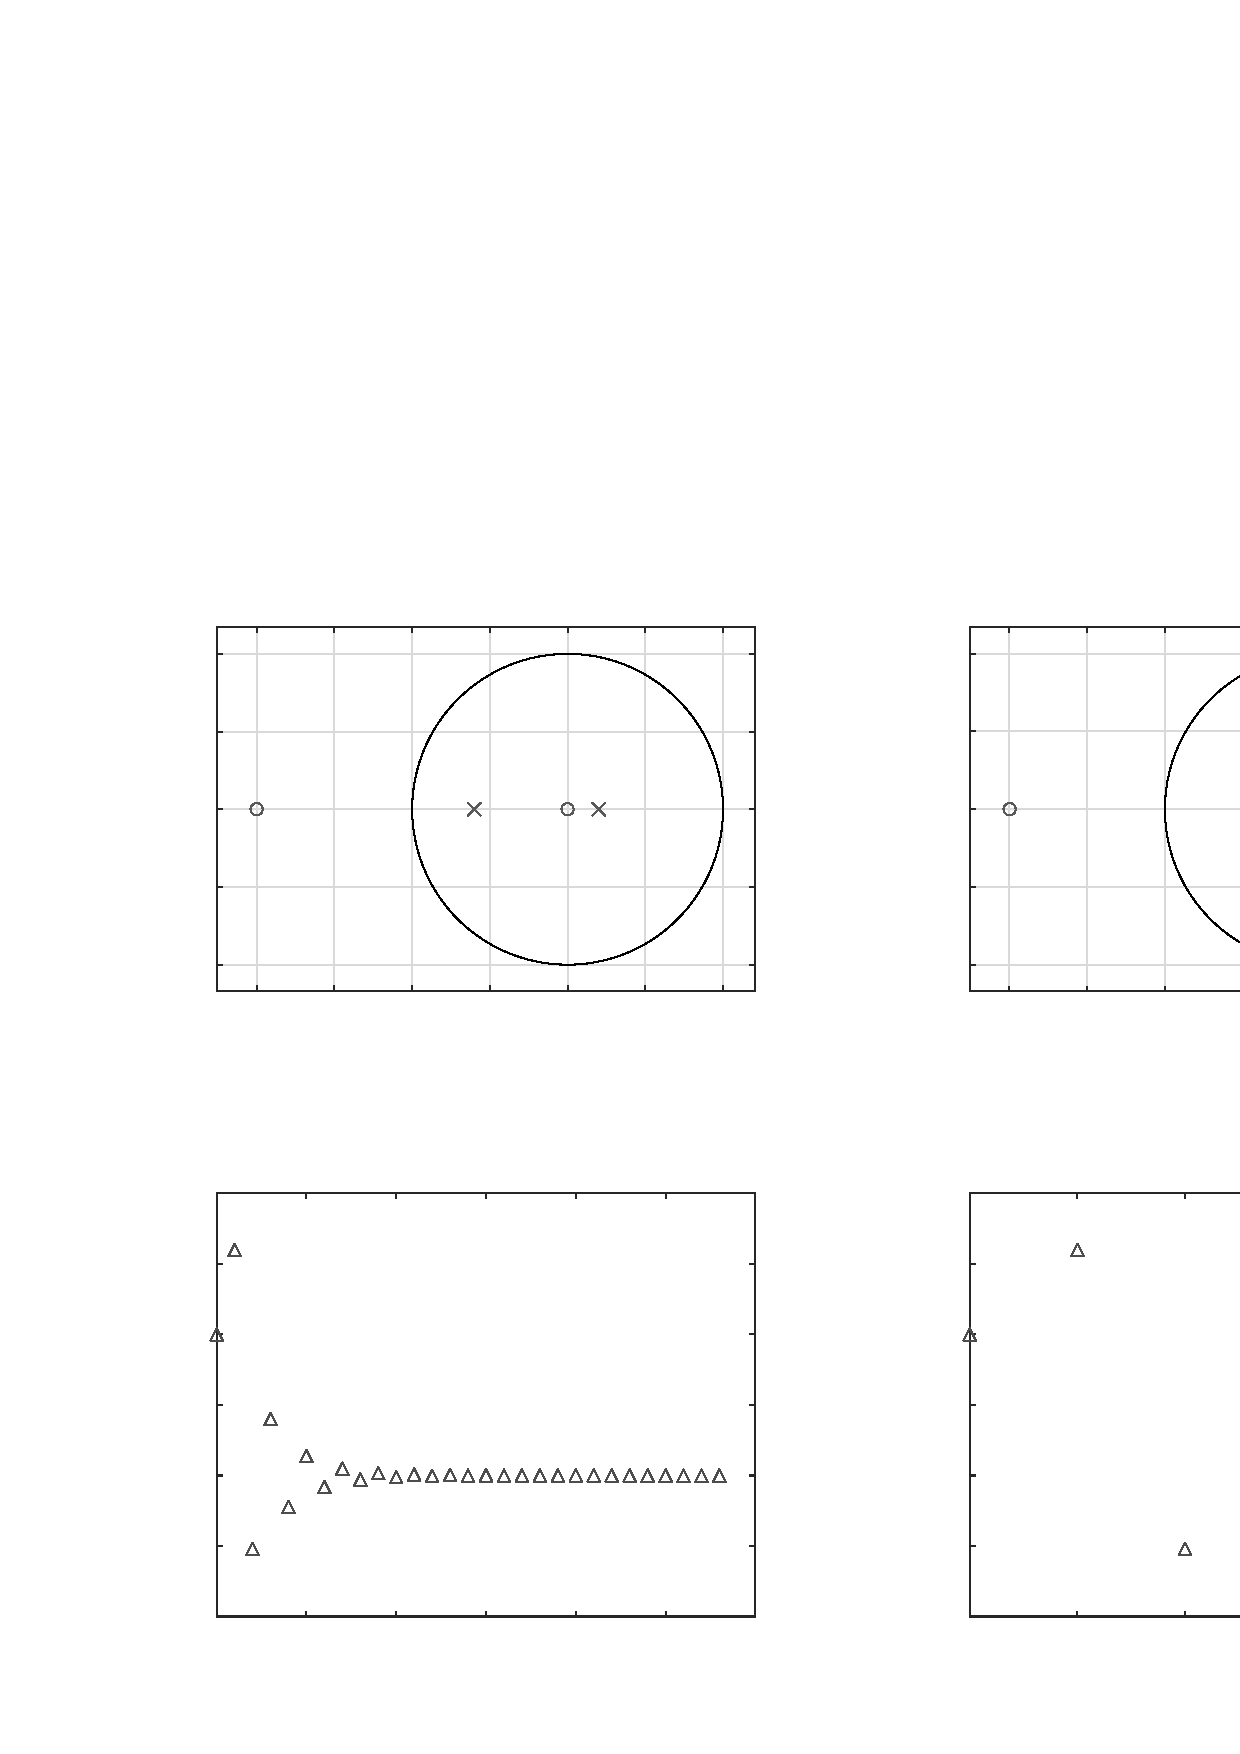
\includegraphics[scale=1]{octaves/zTransform1-inc}
\end{picture}%
\begin{picture}(800,600)(0,0)
\fontsize{13}{0}\selectfont\put(123.215,355.725){\makebox(0,0)[t]{\textcolor[rgb]{0.15,0.15,0.15}{{-2}}}}
\fontsize{13}{0}\selectfont\put(160.524,355.725){\makebox(0,0)[t]{\textcolor[rgb]{0.15,0.15,0.15}{{-1.5}}}}
\fontsize{13}{0}\selectfont\put(197.834,355.725){\makebox(0,0)[t]{\textcolor[rgb]{0.15,0.15,0.15}{{-1}}}}
\fontsize{13}{0}\selectfont\put(235.144,355.725){\makebox(0,0)[t]{\textcolor[rgb]{0.15,0.15,0.15}{{-0.5}}}}
\fontsize{13}{0}\selectfont\put(272.453,355.725){\makebox(0,0)[t]{\textcolor[rgb]{0.15,0.15,0.15}{{0}}}}
\fontsize{13}{0}\selectfont\put(309.763,355.725){\makebox(0,0)[t]{\textcolor[rgb]{0.15,0.15,0.15}{{0.5}}}}
\fontsize{13}{0}\selectfont\put(347.073,355.725){\makebox(0,0)[t]{\textcolor[rgb]{0.15,0.15,0.15}{{1}}}}
\fontsize{13}{0}\selectfont\put(97.0766,378.852){\makebox(0,0)[r]{\textcolor[rgb]{0.15,0.15,0.15}{{-1}}}}
\fontsize{13}{0}\selectfont\put(97.0766,416.162){\makebox(0,0)[r]{\textcolor[rgb]{0.15,0.15,0.15}{{-0.5}}}}
\fontsize{13}{0}\selectfont\put(97.0766,453.472){\makebox(0,0)[r]{\textcolor[rgb]{0.15,0.15,0.15}{{0}}}}
\fontsize{13}{0}\selectfont\put(97.0766,490.782){\makebox(0,0)[r]{\textcolor[rgb]{0.15,0.15,0.15}{{0.5}}}}
\fontsize{13}{0}\selectfont\put(97.0766,528.091){\makebox(0,0)[r]{\textcolor[rgb]{0.15,0.15,0.15}{{1}}}}
\fontsize{13}{0}\selectfont\put(484.444,355.659){\makebox(0,0)[t]{\textcolor[rgb]{0.15,0.15,0.15}{{-2}}}}
\fontsize{13}{0}\selectfont\put(521.789,355.659){\makebox(0,0)[t]{\textcolor[rgb]{0.15,0.15,0.15}{{-1.5}}}}
\fontsize{13}{0}\selectfont\put(559.133,355.659){\makebox(0,0)[t]{\textcolor[rgb]{0.15,0.15,0.15}{{-1}}}}
\fontsize{13}{0}\selectfont\put(596.478,355.659){\makebox(0,0)[t]{\textcolor[rgb]{0.15,0.15,0.15}{{-0.5}}}}
\fontsize{13}{0}\selectfont\put(633.823,355.659){\makebox(0,0)[t]{\textcolor[rgb]{0.15,0.15,0.15}{{0}}}}
\fontsize{13}{0}\selectfont\put(671.168,355.659){\makebox(0,0)[t]{\textcolor[rgb]{0.15,0.15,0.15}{{0.5}}}}
\fontsize{13}{0}\selectfont\put(708.513,355.659){\makebox(0,0)[t]{\textcolor[rgb]{0.15,0.15,0.15}{{1}}}}
\fontsize{13}{0}\selectfont\put(458.52,378.782){\makebox(0,0)[r]{\textcolor[rgb]{0.15,0.15,0.15}{{-1}}}}
\fontsize{13}{0}\selectfont\put(458.52,416.127){\makebox(0,0)[r]{\textcolor[rgb]{0.15,0.15,0.15}{{-0.5}}}}
\fontsize{13}{0}\selectfont\put(458.52,453.472){\makebox(0,0)[r]{\textcolor[rgb]{0.15,0.15,0.15}{{0}}}}
\fontsize{13}{0}\selectfont\put(458.52,490.817){\makebox(0,0)[r]{\textcolor[rgb]{0.15,0.15,0.15}{{0.5}}}}
\fontsize{13}{0}\selectfont\put(458.52,528.162){\makebox(0,0)[r]{\textcolor[rgb]{0.15,0.15,0.15}{{1}}}}
%\fontsize{13}{0}\selectfont\put(633.823,453.472){\makebox(0,0)[l]{\textcolor[rgb]{0.34524,0.34524,0.34524}{{ $^5$}}}}
\fontsize{13}{0}\selectfont\put(104,55.5941){\makebox(0,0)[t]{\textcolor[rgb]{0.15,0.15,0.15}{{0}}}}
\fontsize{13}{0}\selectfont\put(147.093,55.5941){\makebox(0,0)[t]{\textcolor[rgb]{0.15,0.15,0.15}{{5}}}}
\fontsize{13}{0}\selectfont\put(190.185,55.5941){\makebox(0,0)[t]{\textcolor[rgb]{0.15,0.15,0.15}{{10}}}}
\fontsize{13}{0}\selectfont\put(233.278,55.5941){\makebox(0,0)[t]{\textcolor[rgb]{0.15,0.15,0.15}{{15}}}}
\fontsize{13}{0}\selectfont\put(276.371,55.5941){\makebox(0,0)[t]{\textcolor[rgb]{0.15,0.15,0.15}{{20}}}}
\fontsize{13}{0}\selectfont\put(319.464,55.5941){\makebox(0,0)[t]{\textcolor[rgb]{0.15,0.15,0.15}{{25}}}}
\fontsize{13}{0}\selectfont\put(362.556,55.5941){\makebox(0,0)[t]{\textcolor[rgb]{0.15,0.15,0.15}{{30}}}}
\fontsize{13}{0}\selectfont\put(97.0766,66){\makebox(0,0)[r]{\textcolor[rgb]{0.15,0.15,0.15}{{-1}}}}
\fontsize{13}{0}\selectfont\put(97.0766,99.8427){\makebox(0,0)[r]{\textcolor[rgb]{0.15,0.15,0.15}{{-0.5}}}}
\fontsize{13}{0}\selectfont\put(97.0766,133.685){\makebox(0,0)[r]{\textcolor[rgb]{0.15,0.15,0.15}{{0}}}}
\fontsize{13}{0}\selectfont\put(97.0766,167.528){\makebox(0,0)[r]{\textcolor[rgb]{0.15,0.15,0.15}{{0.5}}}}
\fontsize{13}{0}\selectfont\put(97.0766,201.371){\makebox(0,0)[r]{\textcolor[rgb]{0.15,0.15,0.15}{{1}}}}
\fontsize{13}{0}\selectfont\put(97.0766,235.214){\makebox(0,0)[r]{\textcolor[rgb]{0.15,0.15,0.15}{{1.5}}}}
\fontsize{13}{0}\selectfont\put(97.0766,269.056){\makebox(0,0)[r]{\textcolor[rgb]{0.15,0.15,0.15}{{2}}}}
\fontsize{13}{0}\selectfont\put(465.444,55.5941){\makebox(0,0)[t]{\textcolor[rgb]{0.15,0.15,0.15}{{0}}}}
\fontsize{13}{0}\selectfont\put(517.155,55.5941){\makebox(0,0)[t]{\textcolor[rgb]{0.15,0.15,0.15}{{1}}}}
\fontsize{13}{0}\selectfont\put(568.866,55.5941){\makebox(0,0)[t]{\textcolor[rgb]{0.15,0.15,0.15}{{2}}}}
\fontsize{13}{0}\selectfont\put(620.577,55.5941){\makebox(0,0)[t]{\textcolor[rgb]{0.15,0.15,0.15}{{3}}}}
\fontsize{13}{0}\selectfont\put(672.289,55.5941){\makebox(0,0)[t]{\textcolor[rgb]{0.15,0.15,0.15}{{4}}}}
\fontsize{13}{0}\selectfont\put(724,55.5941){\makebox(0,0)[t]{\textcolor[rgb]{0.15,0.15,0.15}{{5}}}}
\fontsize{13}{0}\selectfont\put(458.52,66){\makebox(0,0)[r]{\textcolor[rgb]{0.15,0.15,0.15}{{-1}}}}
\fontsize{13}{0}\selectfont\put(458.52,99.8427){\makebox(0,0)[r]{\textcolor[rgb]{0.15,0.15,0.15}{{-0.5}}}}
\fontsize{13}{0}\selectfont\put(458.52,133.685){\makebox(0,0)[r]{\textcolor[rgb]{0.15,0.15,0.15}{{0}}}}
\fontsize{13}{0}\selectfont\put(458.52,167.528){\makebox(0,0)[r]{\textcolor[rgb]{0.15,0.15,0.15}{{0.5}}}}
\fontsize{13}{0}\selectfont\put(458.52,201.371){\makebox(0,0)[r]{\textcolor[rgb]{0.15,0.15,0.15}{{1}}}}
\fontsize{13}{0}\selectfont\put(458.52,235.214){\makebox(0,0)[r]{\textcolor[rgb]{0.15,0.15,0.15}{{1.5}}}}
\fontsize{13}{0}\selectfont\put(458.52,269.056){\makebox(0,0)[r]{\textcolor[rgb]{0.15,0.15,0.15}{{2}}}}
\end{picture}

    }\caption{Zeroes and poles of $G(z) = \frac{1 - 2z^{-1}}{1 + 0.4z^{-1} - 0.12z^{-2}}$ and of its FIR approximation (above), the related impulse responses (below). To obtain the length-$6$ FIR approximation from the numerator and the denominator of the $z$-transform, run \texttt{num2 = impz(num1,den1,6)', den2 = 1;} octave code. Complete code can be found in file \texttt{zTransform1.m}.}\label{oct:zTransform1}
\end{center}
\end{figure*}

\begin{figure*}[ht]
\begin{center}
\scalebox{0.4}{
% Title: gl2ps_renderer figure
% Creator: GL2PS 1.4.2, (C) 1999-2020 C. Geuzaine
% For: Octave
% CreationDate: Wed Nov  2 14:36:59 2022
\setlength{\unitlength}{1pt}
\begin{picture}(0,0)
\includegraphics[scale=1]{octaves/zTransform2-inc}
\end{picture}%
\begin{picture}(800,600)(0,0)
\fontsize{13}{0}\selectfont\put(373.458,148.96){\makebox(0,0)[tl]{\textcolor[rgb]{0.15,0.15,0.15}{{2}}}}
\fontsize{13}{0}\selectfont\put(314.939,110.968){\makebox(0,0)[tl]{\textcolor[rgb]{0.15,0.15,0.15}{{0}}}}
\fontsize{13}{0}\selectfont\put(344.198,129.964){\makebox(0,0)[tl]{\textcolor[rgb]{0.15,0.15,0.15}{{1}}}}
\fontsize{13}{0}\selectfont\put(93.0986,228.825){\makebox(0,0)[br]{\textcolor[rgb]{0.15,0.15,0.15}{{-4}}}}
\fontsize{13}{0}\selectfont\put(146.501,119.043){\makebox(0,0)[tr]{\textcolor[rgb]{0.15,0.15,0.15}{{0}}}}
\fontsize{13}{0}\selectfont\put(127.791,139.673){\makebox(0,0)[tr]{\textcolor[rgb]{0.15,0.15,0.15}{{0.5}}}}
\fontsize{13}{0}\selectfont\put(109.081,160.303){\makebox(0,0)[tr]{\textcolor[rgb]{0.15,0.15,0.15}{{1}}}}
\fontsize{13}{0}\selectfont\put(90.3716,180.933){\makebox(0,0)[tr]{\textcolor[rgb]{0.15,0.15,0.15}{{1.5}}}}
\fontsize{13}{0}\selectfont\put(165.211,98.4124){\makebox(0,0)[tr]{\textcolor[rgb]{0.15,0.15,0.15}{{-0.5}}}}
\fontsize{13}{0}\selectfont\put(183.92,77.7823){\makebox(0,0)[tr]{\textcolor[rgb]{0.15,0.15,0.15}{{-1}}}}
\fontsize{13}{0}\selectfont\put(202.63,57.1521){\makebox(0,0)[tr]{\textcolor[rgb]{0.15,0.15,0.15}{{-1.5}}}}
\fontsize{13}{0}\selectfont\put(227.16,53.9797){\makebox(0,0)[tl]{\textcolor[rgb]{0.15,0.15,0.15}{{-3}}}}
\fontsize{13}{0}\selectfont\put(256.419,72.9758){\makebox(0,0)[tl]{\textcolor[rgb]{0.15,0.15,0.15}{{-2}}}}
\fontsize{13}{0}\selectfont\put(285.679,91.9719){\makebox(0,0)[tl]{\textcolor[rgb]{0.15,0.15,0.15}{{-1}}}}
\fontsize{13}{0}\selectfont\put(93.0986,282.873){\makebox(0,0)[br]{\textcolor[rgb]{0.15,0.15,0.15}{{-2}}}}
\fontsize{13}{0}\selectfont\put(93.0986,336.921){\makebox(0,0)[br]{\textcolor[rgb]{0.15,0.15,0.15}{{0}}}}
\fontsize{13}{0}\selectfont\put(93.0986,390.968){\makebox(0,0)[br]{\textcolor[rgb]{0.15,0.15,0.15}{{2}}}}
\fontsize{13}{0}\selectfont\put(93.0986,445.016){\makebox(0,0)[br]{\textcolor[rgb]{0.15,0.15,0.15}{{4}}}}
\fontsize{13}{0}\selectfont\put(705.642,129.964){\makebox(0,0)[tl]{\textcolor[rgb]{0.15,0.15,0.15}{{1}}}}
\fontsize{13}{0}\selectfont\put(454.542,228.825){\makebox(0,0)[br]{\textcolor[rgb]{0.15,0.15,0.15}{{-4}}}}
\fontsize{13}{0}\selectfont\put(676.382,110.968){\makebox(0,0)[tl]{\textcolor[rgb]{0.15,0.15,0.15}{{0}}}}
\fontsize{13}{0}\selectfont\put(451.815,180.933){\makebox(0,0)[tr]{\textcolor[rgb]{0.15,0.15,0.15}{{1.5}}}}
\fontsize{13}{0}\selectfont\put(470.525,160.303){\makebox(0,0)[tr]{\textcolor[rgb]{0.15,0.15,0.15}{{1}}}}
\fontsize{13}{0}\selectfont\put(489.235,139.673){\makebox(0,0)[tr]{\textcolor[rgb]{0.15,0.15,0.15}{{0.5}}}}
\fontsize{13}{0}\selectfont\put(507.944,119.043){\makebox(0,0)[tr]{\textcolor[rgb]{0.15,0.15,0.15}{{0}}}}
\fontsize{13}{0}\selectfont\put(526.654,98.4124){\makebox(0,0)[tr]{\textcolor[rgb]{0.15,0.15,0.15}{{-0.5}}}}
\fontsize{13}{0}\selectfont\put(545.364,77.7823){\makebox(0,0)[tr]{\textcolor[rgb]{0.15,0.15,0.15}{{-1}}}}
\fontsize{13}{0}\selectfont\put(564.074,57.1521){\makebox(0,0)[tr]{\textcolor[rgb]{0.15,0.15,0.15}{{-1.5}}}}
\fontsize{13}{0}\selectfont\put(588.603,53.9797){\makebox(0,0)[tl]{\textcolor[rgb]{0.15,0.15,0.15}{{-3}}}}
\fontsize{13}{0}\selectfont\put(617.863,72.9758){\makebox(0,0)[tl]{\textcolor[rgb]{0.15,0.15,0.15}{{-2}}}}
\fontsize{13}{0}\selectfont\put(647.123,91.9719){\makebox(0,0)[tl]{\textcolor[rgb]{0.15,0.15,0.15}{{-1}}}}
\fontsize{13}{0}\selectfont\put(734.901,148.96){\makebox(0,0)[tl]{\textcolor[rgb]{0.15,0.15,0.15}{{2}}}}
\fontsize{13}{0}\selectfont\put(454.542,282.873){\makebox(0,0)[br]{\textcolor[rgb]{0.15,0.15,0.15}{{-2}}}}
\fontsize{13}{0}\selectfont\put(454.542,336.921){\makebox(0,0)[br]{\textcolor[rgb]{0.15,0.15,0.15}{{0}}}}
\fontsize{13}{0}\selectfont\put(454.542,390.968){\makebox(0,0)[br]{\textcolor[rgb]{0.15,0.15,0.15}{{2}}}}
\fontsize{13}{0}\selectfont\put(454.542,445.016){\makebox(0,0)[br]{\textcolor[rgb]{0.15,0.15,0.15}{{4}}}}
\end{picture}

    }\caption{Plot of $G(z) = \frac{1 - 2z^{-1}}{1 + 0.4z^{-1} - 0.12z^{-2}}$ (left) and of its FIR approximation (right). Notice the correspondence between these two plots and the location of zeros and poles in Figure~\ref{oct:zTransform1}.}\label{oct:zTransform2}
\end{center}
\end{figure*}

Generally speaking, if the rational $z$-transform has $N$ poles with $R$, then there are $R+1$ regions of convergence, that will all change as poles do. There are, in fact, $R+1$ distinct sequences with the same $z$-transform formula, but with different RoC. For this reason, a rational $z$-transform with a specified region of convergence will possess a unique sequence as its $z$-transform.

The region of convergence of a rational $z$-transform can be soon determined using \texttt{octave} with the function call
\begin{verbatim}
[z, p, k] = tf2zp(num, den);
\end{verbatim}
which determines the zeros, poles and the gain constant of a rational $z$-transform expressed by the vectors \texttt{num} and \texttt{den}, two vectors carrying---respectively---the numerator and the denominator of the rational $z$-transform. Reverse process can be obtained by simply calling the inverse function
\begin{verbatim}
[num, den] = zp2tf(z, p, k);
\end{verbatim}
whose return values will represent a rational $z$-transform expressed by numerator and denominator vectors \texttt{num} and \texttt{den}.

The factored form of the $z$-transform, as in~\ref{eqn:rationalzTransformFactored}, can be collected by means of
\begin{verbatim}
sos = zp2sos(z, p, k);
\end{verbatim}
computing the coefficients of each second-order factor given as an $L \times 6$ matrix \texttt{sos}, where
\[
    sos =
    \begin{bmatrix}
        b_{01} & b_{11} & b_{21} & a_{01} & a_{11} & a_{21} \\
        b_{02} & b_{12} & b_{22} & a_{02} & a_{12} & a_{22} \\
        \vdots & \vdots & \vdots & \vdots & \vdots & \vdots \\
        b_{0L} & b_{1L} & b_{2L} & a_{0L} & a_{1L} & a_{1L}
    \end{bmatrix}
\]
where factors are of the $2$nd order and are expressed as follows,
\begin{equation}\label{eqn:rationalzTransformFactoredSecondOrder}
    G(z) = \prod_{k=1}^L\frac{
        b_{0k} + b_{1k}z^{-1} + b_{2k}z^{-2}
    } {
        a_{0k} + a_{1k}z^{-1} + a_{2k}z^{-2}
    }.
\end{equation}

To determine the zero-pole plane, use the function \texttt{zplane}, either by providing \texttt{zplane(zeros, poles)} or by calling it with numerator and denominator vectors \texttt{zplane(num, den)}. Vectors \texttt{zeros}, \texttt{poles} are both column vectors, while on contrary vectors \texttt{num} and \texttt{den} are row vectors.

For instance, let a rational $z$-transform function be defined as such,
\[
    J(z) = \frac{
        2z^4 + 16z^3 + 44z^2 + 56z + 32
    } {
        3z^4 + 3z^3 - 15z^2 + 18z - 12
    };
\]
to describe it in terms of numerator and denominator vectors, one can run
\begin{verbatim}
pkg load signal;
num = [2 16 44 56 32];
den = [3 3 -15 18 -12];
zplane(num, den);
\end{verbatim}
which will generate a z-plane plot with zeros and poles drawn at their location in the plane, as in Figure~\ref{oct:poleZeroPlotExample}.

\begin{figure*}[ht]
\begin{center}
\scalebox{0.3}{
% Title: gl2ps_renderer figure
% Creator: GL2PS 1.4.2, (C) 1999-2020 C. Geuzaine
% For: Octave
% CreationDate: Thu Nov  3 08:42:14 2022
\setlength{\unitlength}{1pt}
\begin{picture}(0,0)
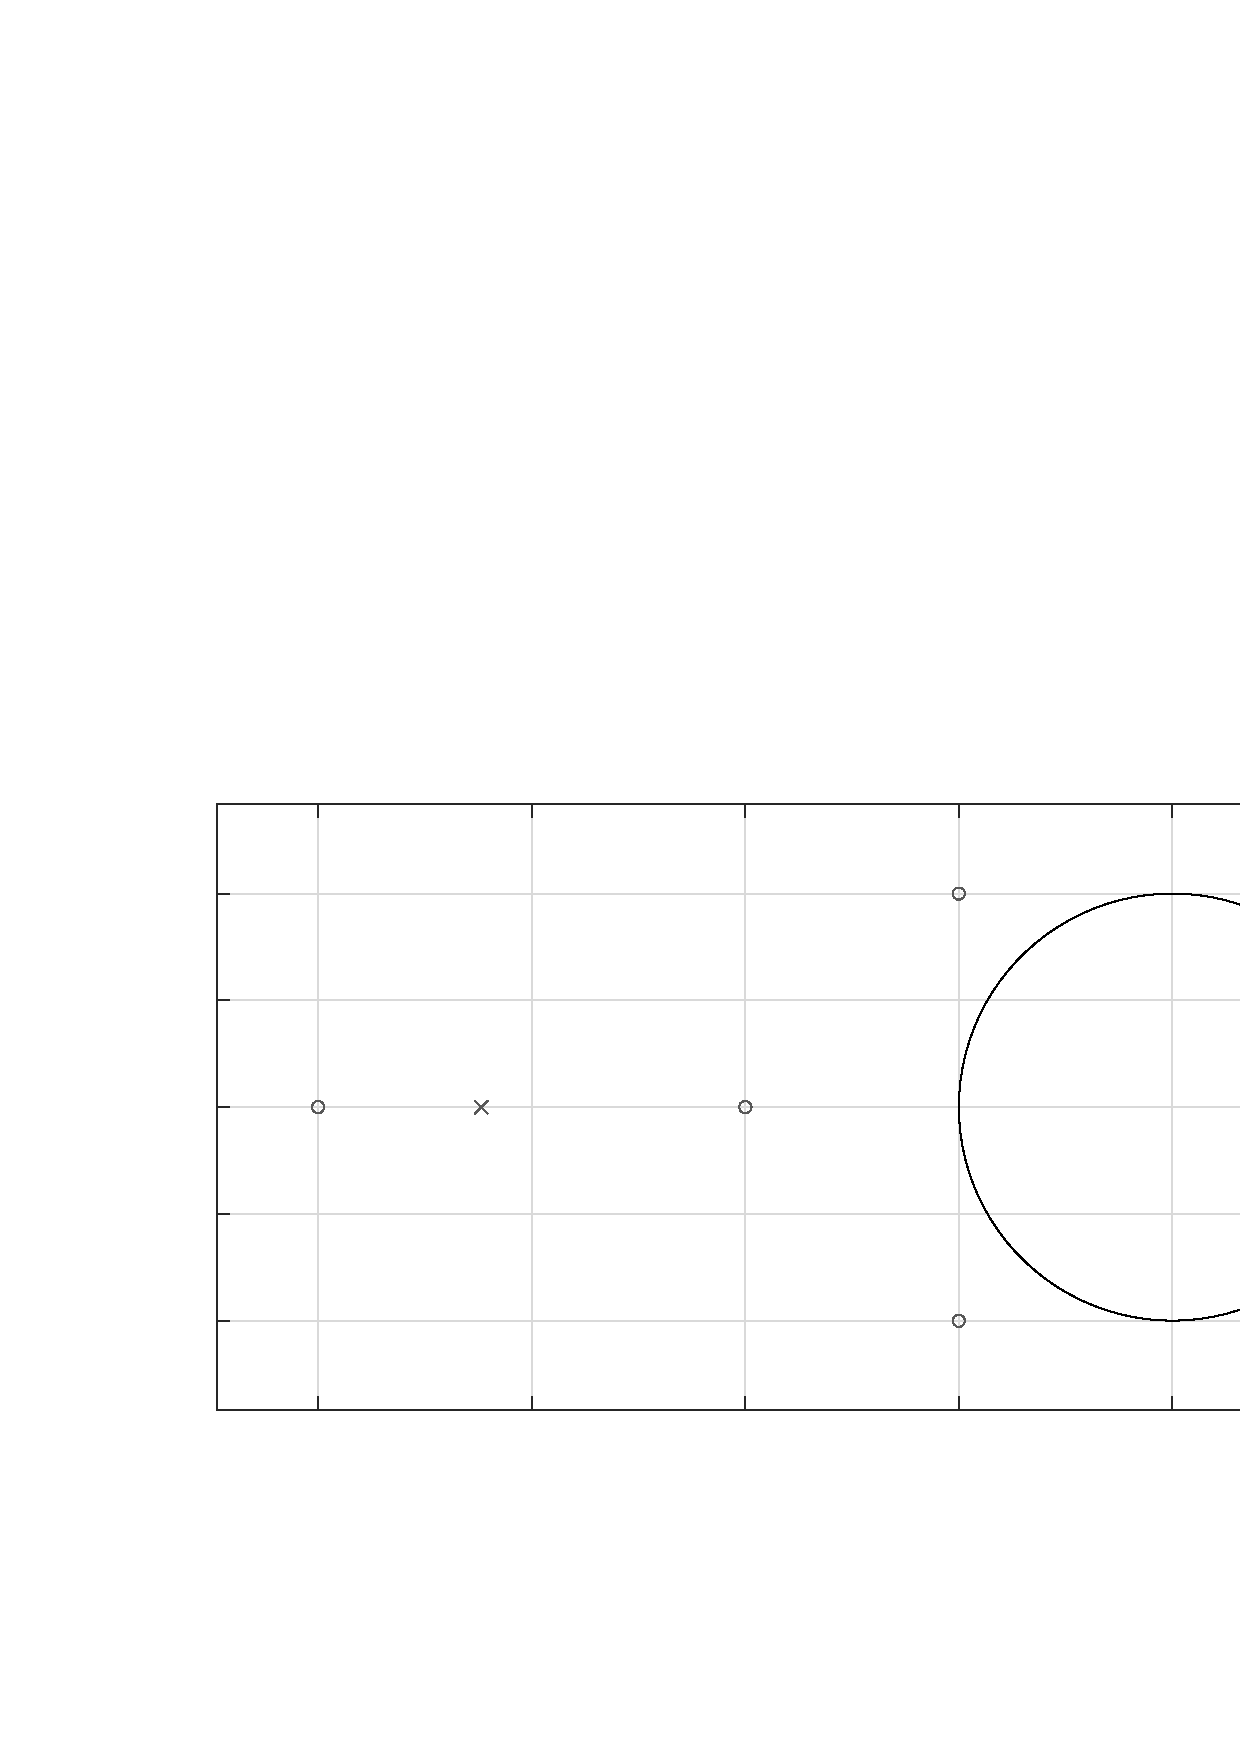
\includegraphics[scale=1]{octaves/poleZeroPlotExample-inc}
\end{picture}%
\begin{picture}(800,600)(0,0)
\fontsize{13}{0}\selectfont\put(152.686,154.795){\makebox(0,0)[t]{\textcolor[rgb]{0.15,0.15,0.15}{{-4}}}}
\fontsize{13}{0}\selectfont\put(255.205,154.795){\makebox(0,0)[t]{\textcolor[rgb]{0.15,0.15,0.15}{{-3}}}}
\fontsize{13}{0}\selectfont\put(357.724,154.795){\makebox(0,0)[t]{\textcolor[rgb]{0.15,0.15,0.15}{{-2}}}}
\fontsize{13}{0}\selectfont\put(460.243,154.795){\makebox(0,0)[t]{\textcolor[rgb]{0.15,0.15,0.15}{{-1}}}}
\fontsize{13}{0}\selectfont\put(562.762,154.795){\makebox(0,0)[t]{\textcolor[rgb]{0.15,0.15,0.15}{{0}}}}
\fontsize{13}{0}\selectfont\put(665.281,154.795){\makebox(0,0)[t]{\textcolor[rgb]{0.15,0.15,0.15}{{1}}}}
\fontsize{13}{0}\selectfont\put(97.0525,207.981){\makebox(0,0)[r]{\textcolor[rgb]{0.15,0.15,0.15}{{-1}}}}
\fontsize{13}{0}\selectfont\put(97.0525,259.24){\makebox(0,0)[r]{\textcolor[rgb]{0.15,0.15,0.15}{{-0.5}}}}
\fontsize{13}{0}\selectfont\put(97.0525,310.5){\makebox(0,0)[r]{\textcolor[rgb]{0.15,0.15,0.15}{{0}}}}
\fontsize{13}{0}\selectfont\put(97.0525,361.759){\makebox(0,0)[r]{\textcolor[rgb]{0.15,0.15,0.15}{{0.5}}}}
\fontsize{13}{0}\selectfont\put(97.0525,413.019){\makebox(0,0)[r]{\textcolor[rgb]{0.15,0.15,0.15}{{1}}}}
\end{picture}

}\caption{Plot of z-plane zeros and poles of function
$J(z) = \frac{
        2z^4 + 16z^3 + 44z^2 + 56z + 32
    } {
        3z^4 + 3z^3 - 15z^2 + 18z - 12
    }$.
}\label{oct:poleZeroPlotExample}
\end{center}
\end{figure*}

\clearpage

\section{Inverse $z$-Transform}

Now that we had dealt with $z$-transform properties, region of convergence, notable transforms and rational $z$-transforms alternative forms, it is the time to finally introduce the \textbf{Inverse $z$-Transform}.

A $z$-transform is generally given by the formula
\[
    G(z) = \sum_{n=-\infty}^\infty g[n]z^{-n} = \sum_{n=-\infty}^\infty g[n]r^{-n}e^{-j\omega n}
\]
with $z=re^{j\omega}$, is solely the Discrete-time Fourier Transform of the modified sequence $g[n]r^{-n}$. Subsequently, the inverse DTFT is given by
\[
    g[n]r^{-n} = \frac 1 {2\pi} \int_{-\pi}^\pi G(re^{j\omega}) e^{j\omega n} d\omega.
\]

Following the same idea as above, by making a variable change $z=re^{j\omega}$ the previous equation should yield the formula for the inverse $z$-transform. In point of fact, the above grows into a contour integral, giben by the following
\begin{equation}\label{eqn:inversezTransform}
    g[n] = \frac{1}{2j\pi}\oint_\gamma G(z) z^{n-1}dz
\end{equation}
where $\gamma$ is a \emph{counterclockwise contour of integration} defined by $|z| = r$. The integral value remains unchanged when $\gamma$ is replaced with any contour $\zeta$ surrounding point $z = 0$ and going through the region of convergence of $G(z)$, so
\[
    g[n] = \frac{1}{2j\pi}\oint_\zeta G(z) z^{n-1}dz.
\]
This means that the contour integral can be soon evaluated by means of the \emph{Cauchy's residue theorem} resulting in a sum of \emph{residues}
\[
    g[n] = \sum\left[ \makecell{ \mbox{ residues of } G(z)z^{n-1} \\ \mbox{ at the poles inside } \zeta} \right].
\]

In reality, the above integration is merely a conceptual step, rather than an actual method for inversion that should be adopted. In fact, inversion is usually performed through the \textbf{Partial-Fraction Expansion}. This method draws its core idea from the fact that any rational $z$-transform $G(z)$ with a causal inverse transform $g[n]$ has a RoC that is exterior to a circle: it is more convenient to express $G(z)$ in a \emph{partial-fraction expansion} form and then determine $g[n]$ by summing the inverse transform of the individual simpler terms in the expansion. The trick here is to somehow make the rational form \emph{simpler} by splitting it into smaller terms, each one with their own simpler inverse transform, and summing up all together in the end.

As we have already seen, rational $G(z)$ functions can be expressed as follows,
\[
    G(z) = \frac{P(z)}{D(z)} =
    \frac {
        \sum_{i=0}^M p_i z^{-i}
    } {
        \sum_{i=0}^N d_i z^{-i}
    }.
\]

However, if $M\leq N$, then $G(z)$ can be rewritten as
\begin{equation}\label{eqn:partialFractionExpansion}
    G(z) = \sum_{l=0}^{M-N} \eta_l z^{-l} + \underbrace{\frac{P'(z)}{D(z)}}_{\Upsilon(z)},
\end{equation}
where the degree of $P'(z)$ is \emph{less} than the original degree $N$.
The rational function $\Upsilon(z) := \frac{P'(z)}{D(z)}$ is called \emph{proper fraction}. The proper fraction part $\Upsilon(z)$ can be developed from $G(z)$ by performing a long division between $P(z)$ and $D(z)$ in a reverse order until the remainder polynomial $P'(z)$is of a lower degree than that of the denominator---a technique called \textbf{method of residues}.

Indeed, one can employ \textsc{Octave}'s command \texttt{residuez} to compute the partial-fraction expansion of a rational $z$-transform with numerator and denominator coefficients given by vectors \texttt{num} and \texttt{den},
\begin{verbatim}
[r, p, k] = residuez(num, den)
\end{verbatim}
For example,
\begin{verbatim}
pkg load signal;
num = [2 16 44 56 32];
den = [3 3 -15 18 -12];
[r, p, k] = residuez(num, den)
\end{verbatim}
yields
\begin{verbatim}
r =

  -3.070175 - 2.339788i
  -3.070175 + 2.339788i
   9.491429 - 0.000000i
  -0.017745 + 0.000000i

p =

   0.5000 - 0.8660i
   0.5000 + 0.8660i
   1.2361 +      0i
  -3.2361 -      0i

k = -2.6667
\end{verbatim}

Vector \texttt{r} contains the residues, vector \texttt{p} contains the poles, while vector \texttt{k} encloses the constants $\eta_l$. The inverse process is performed by the same function invocation, with converse arguments:
\begin{verbatim}
[num, den] = residuez(r, p, k)
\end{verbatim}
which converts a $z$-transform expressed in partial-fraction expansion form to its rational form.

\subsection{Inverse $z$-Transform using Long Division}

\textbf{Long division} can be employed to actually compute the $z$-transform. Verily, the $z$-transform $G(z)$ of $\{g[n]\}$ can be expanded in a power series $z^{-1}$, and in such series expansion the coefficient multiplying term $z^{-n}$ is the $n$-th sample $g[n]$. For rational $z$-transforms expressed as ratio of polynomials in $z^{-1}$ the power series expansion can be obtained by long division in the following manner.

Let
\[
    H(z) = \frac {
        1 + 2z^{-1}
    } {
        1 + 0.4z^{-1} - 0.12z^{-2}
    };
\]
long division of the numerator by the denominator yields the rewriting of $H(z)$ into its \emph{FIR approximation}
\[
    H(z) = 1 + 1.6z^{-1} - 0.52z^{-2} + 0.4z^{-3} - 0.2224z^{-4} + \cdots
\]
where the $\dots$ signify that among the infinite sum only values up to term $z^{-4}$ were collected. The resulting causal sequence will be
\[
    \{h[n]\} =
    \begin{Bmatrix} 
        1 & 1.6z^{-1} - 0.52z^{-2} & 0.4z^{-3} - 0.2224z^{-4} & \cdots
    \end{Bmatrix}
\]

The function \texttt{impz} can be used to find the inverse of a rational $z$-transform $G(z)$: it computes the coefficients of the power series expansion of $G(z)$, only gathering a specified or automatically-determined amount of coefficients.

The following Table~\ref{tab:zTransformTheorems} summarizes the most crucial theorems and results.

\begin{table*}[ht]
\centering
\begin{tabular}{l|ccc}
    \textbf{Theorem} & \textbf{Sequence} & \textbf{$z$-Transform} & \textbf{RoC} \\
    \hline
    Conjugation & $g^*[n]$ & $G^*(z^*)$ & $\mathcal R_g$\\
    Time-reversal & $g[-n]$ & $G(\frac{1}{z})$ & $\frac{1}{\mathcal R_g}$\\
    Linearity & $\alpha g[n] + \beta h[n]$ & $\alpha G(z) + \beta H(z)$ & \makecell{Includes\\ $\mathcal R_g \cup \mathcal R_h$}\\
    Time-shifting & $g[n - n_0]$ & $z^{-n_0}G(z)$ & \makecell{$\mathcal R_g$ except possibly\\ point $z=0$ or $z = \infty$}\\
    Multiplication by exponential sequence & $\alpha^n g[n]$ & $G(\frac z \alpha)$ & $|\alpha|\mathcal R_g$\\
    Differentiation of $G(z)$ & $n g[n]$ & $-z\frac{dG(z)}{dz}$ & \makecell{$\mathcal R_g$, except\\ possibly $z=0$ or $z=\infty$}\\
    Convolution & $g[n] \circledast h[n]$ & $G(z)\cdot H(z)$ & \makecell{Includes\\ $\mathcal R_g \cup \mathcal R_h$}\\
    Modulation & $g[n] \cdot h[n]$ & $\frac{1}{2\pi j} \oint_\gamma G(\upsilon)\cdot H(\frac{z}{\upsilon})\upsilon^{-1} d\upsilon$ & \makecell{Includes\\ $\mathcal R_g \mathcal R_h$}\\
    \hline
    Parseval's relation & \makecell{$\sum_{n=-\infty}^\infty g[n]h^*[n] =$ \\ $= \frac{1}{2\pi j} \oint_\gamma G(\upsilon)\cdot H(\frac{z}{\upsilon})\upsilon^{-1} d\upsilon$} & &
\end{tabular}
    \caption{If $\mathcal R_g$ denotes the region of convergence $\mathcal R_{g-} < |z| < \mathcal R_{g+}$ and $\mathcal R_h$ denotes the region of convergence $\mathcal R_{h-} < |z| < \mathcal R_{h+}$, then $\frac{1}{\mathcal R_{g+}}$ denotes the region $\frac{1}{\mathcal R_{g-}} < |z| < \frac{1}{\mathcal R_{g+}}$ and the region $\mathcal R_g \mathcal R_h$ denotes the region $\mathcal R_{g-}\mathcal R_{h-} < |z| < \mathcal R_{g+}\mathcal R_{h+}$.}\label{tab:zTransformTheorems}
\end{table*}

\section{Examples of $z$-Transform calculus}
Let $x_1[n]$ be a causal sequence such as\cite{bib:zTransformExamples}
\[
    x_1[n] = \left(\frac 1 2\right)^n \mu[n] + \left(-\frac 1 4\right)^n \mu[n] = a[n] + b[n].
\]
The $z$-transform of $\left(\frac 1 2\right)^n \mu[n]$ is
\[
    A(z) = \frac{z}{z-\frac 1 2},
\]
which yields a RoC of $|z| > \frac 1 2$. Similarly, the $z$-transform of the other addendum $\left(-\frac 1 4\right)^n \mu[n]$ is
\[
    B(z) = \frac{z}{z+\frac 1 4}
\]
possessing a RoC of $|z| > - \frac 1 4$. The two regions of convergence, then, will be like in the following plot,
\begin{center}
    \begin{tikzpicture}
        \draw[thick,-stealth] (-2.5,0) -- (2.5,0) node[anchor=north west] {$\Re z$};
        \draw[thick,-stealth] (0,-2.5) -- (0,2.5) node[anchor=south east] {$\Im z$};
        \node[draw, circle, minimum size=3cm] at (0,0){};
        \node[draw, circle, minimum size=1.5cm] at (0,0){};
        \node[draw, polez, thick] at (1.5, 0) {};
        \node[draw, polez, thick] at (-.75, 0) {};
        \node[label=south east:{$0.5$}, minimum size=0pt] at (1.5, 0) {};
        \node[label=south west:{$0.25$}, minimum size=0pt] at (-.75, 0) {};
        \path[pattern=north west lines, pattern color=red, opacity=.5, even odd rule]
            (-3, -3) rectangle (3,3)
            (0,0) circle[radius=1.5];
        \path[pattern=north east lines, pattern color=green, opacity=.3, even odd rule]
            (-3, -3) rectangle (3,3)
            (0,0) circle[radius=.75];
    \end{tikzpicture}
\end{center}
with red area denoting the RoC of $A(z)$, and the green area denoting the RoC of $B(z)$. Note that the green area and the red area overlaps outside of the circle of radius $|z| = 0.5$. In virtue of the superposition principle, the two $z$-transform can be added together to form $X_1(z) = A(z) + B(z)$. That is,
\begin{align*}
    X_1(z)  &= \frac{z}{z - \frac 1 2} + \frac{z}{z + \frac 1 4} \\
            &= \frac {
                2z \left(z - \frac 1 8\right)
            } {
                \left(z - \frac 1 2\right) \left(z + \frac 1 4\right)
            }.
\end{align*}

By observing at the above result, it is clear that there are two poles, one located at $z=\frac 1 2$ and the other one located at $z = - \frac 1 4$; similarly, there are two zeros, one at the origin and the other one at $z = \frac 1 8$.

Since---for right-sided sequences---the pole that de\-ter\-mi\-nes the region of convergence is the one with the greatest modulus, it immediately follows that the region of convergence is the area $|z| > \frac 1 2$, as depicted in the following illustration (RoC is in blue). From there it is also evident that the DTFT exists, as the region of convergence includes the unit circle.

This was an example of determining the $z$-transform and the RoC of a sequence composed of two right-sided sequences---let's now focus on the case of a sequence embodying a left-sided sequence and a right-sided sequence.

\begin{center}
    \begin{tikzpicture}
        \draw[thick,-stealth] (-3.5,0) -- (3.5,0) node[anchor=north west] {$\Re z$};
        \draw[thick,-stealth] (0,-3.5) -- (0,3.5) node[anchor=south east] {$\Im z$};
        \node[draw, circle, dashed, minimum size=6cm] at (0,0){};
        \node[draw, circle, thick, minimum size=3cm] at (0,0){};
        \node[draw, polez, thick, label=south east:{$\frac 1 2$}] at (1.5, 0) {};
        \node[draw, polez, thick, label=south east:{$\frac 1 4$}] at (-.75, 0) {};
        \node[draw, zeroz, thick, label=south east:{$0$}] at (0, 0) {};
        \node[draw, zeroz, thick, label=south east:{$\frac 1 8$}] at (.375, 0) {};
        \node at (3.1, -0.2) {$1$};
        \path[pattern=north west lines, pattern color=blue, opacity=.5, even odd rule]
            (-3.2, -3.2) rectangle (3.2,3.2)
            (0,0) circle[radius=1.5];
    \end{tikzpicture}
\end{center}

Let then the sequence in exam be
\[
    x_2[n] = \underbrace{\left(-\frac 1 4\right)^n \mu[n]}_{causal} - \underbrace{\left(\frac 1 2\right)^n \mu[-n-1]}_{anticausal} = c[n] + d[n];
\]
first, let's find out the $z$-transforms of the two addenda,
\[
    C(z) = \frac{z}{z + \frac 1 4}, |z| > - \frac 1 4
\]
which means that $C(z) \equiv B(z)$ from the previous example. Regarding the transform of $d[n] = - (\frac 1 2)^n \mu[-n-1]$, one has
\[
    D(z) = \frac{z}{z-\frac 1 2}, |z| < \frac 1 2
\]
because it is a left-sided sequence. Therefore, the RoC of such term will be, plotted as
\begin{center}
    \begin{tikzpicture}
        \draw[thick,-stealth] (-2.5,0) -- (2.5,0) node[anchor=north west] {$\Re z$};
        \draw[thick,-stealth] (0,-2.5) -- (0,2.5) node[anchor=south east] {$\Im z$};
        \node[draw, circle, minimum size=3cm] at (0,0){};
        \node[draw, polez, thick, label=south east:{$\frac 1 2$}] at (1.5, 0) {};
        \path[pattern=north west lines, pattern color=red, opacity=.5, even odd rule]
            (0,0) circle[radius=1.5];
            (-3, -3) rectangle (3,3)
    \end{tikzpicture}
\end{center}

By superposition principle, once again we are able to merge together the above results,
\begin{align*}
    X_2(z)  &= \frac{z}{z + \frac 1 4} + \frac{z}{z - \frac 1 2} \\
            &= \frac {
                z\left(2z - \frac 1 8\right)
            } {
                \left(z + \frac 1 4\right)\left(z - \frac 1 2\right)
            }
\end{align*}

Again by observation one can conclude that there are two poles and two zeros; hence, $z_{p1} = -\frac 1 4$, $z_{p2} = \frac 1 2$, $z_{z1} = \frac 1 8$ and finally the zero at the origin $z_{z2} = 0$. The plot will then be as follows, with the region of converge the annular region in between the two poles.

\begin{center}
    \begin{tikzpicture}
        \draw[thick,-stealth] (-3.5,0) -- (3.5,0) node[anchor=north west] {$\Re z$};
        \draw[thick,-stealth] (0,-3.5) -- (0,3.5) node[anchor=south east] {$\Im z$};
        \node[draw, circle, dashed, minimum size=6cm] at (0,0){};
        \node[draw, circle, thick, minimum size=3cm] at (0,0){};
        \node[draw, circle, thick, minimum size=1.5cm] at (0,0){};
        \node[draw, polez, thick, label=south east:{$\frac 1 2$}] at (+1.5, 0) {};
        \node[draw, polez, thick, label=south east:{$\frac 1 4$}] at (-.75, 0) {};
        \node[draw, zeroz, thick, label=south east:{$\frac 1 8$}] at (.375, 0) {};
        \node[draw, zeroz, thick, label=south east:{$0$}] at (0, 0) {};
        \node at (3.1, -0.2) {$1$};
        \path[pattern=north west lines, pattern color=blue, opacity=.5, even odd rule]
            (-3.2, -3.2) rectangle (3.2,3.2)
            (-3.2, -3.2) rectangle (3.2,3.2)
            (0,0) circle[radius=0.75]
            (0,0) circle[radius=1.5];
    \end{tikzpicture}
\end{center}

Clearly, in order to craft a system that is actually useful by virtue of being causal and BIBO stable, we must ensure that it is within the Region of Convergence, which can be ascertained by looking at the pole zero plot. The Region of Convergence is the area in the pole/zero plot of the transfer function in which the function exists. For purposes of useful filter design, we prefer to work with rational functions, which can be described by two polynomials, one each for determining the poles and the zeros, respectively.

\chapter{Sampling, interpolation, and reconstruction of signals}

In general, only \emph{infinite-length} signals can have \emph{finite band}---since in reality one can only generate a finite-length signal, all signals will, in practice, possess an infinite band. Infinite band signals will see its Fourier Transform (Section~\ref{sec:continuousTimeFourierTransform}) spanning through the entire frequency domain, hence $B \rightarrow \infty$. This is why, in order to sample a finite-length signal it is paramount to first \emph{lowpass filter it}.

\section{Sampling}

Suppose an infinite-length continuous-time signal $f(t)$ is sampled with sampling step $\Delta T$, to obtain a sequence $x[n]$ from it,
\begin{align*}
    x[n] &= f(t) \sum_{n=-\infty}^\infty \delta(t - n\Delta T)\\
         &= \sum_{n=-\infty}^\infty f(t)\delta(t - n \Delta T);
\end{align*}
by \emph{Fourier transforming} the sequence $x[n]$, one obtains
\begin{align*}
    X(f) &= \frac 1 {\Delta T} \int_{-\infty}^\infty F(\tau) \sum_{n=-\infty}^\infty \delta(f - \tau - \frac n {\Delta T})d\tau = \\
         &= \frac 1 {\Delta T} \sum_{n=-\infty}^\infty \int_{-\infty}^\infty F(\tau)  \delta(f - \frac n {\Delta T} - \tau)d\tau = \\
         &= \frac 1 {\Delta T} \sum_{n=-\infty}^\infty F\left(f - \frac{n}{\Delta T}\right) \\
         &= F(f) \circledast S_\delta (f),
\end{align*}
where
\[
    S_\delta(f) = \mathcal F\left\{\sum_{n} \delta(t - n\Delta T)\right\} = \sum_{n=-\infty}^\infty \frac {1}{\Delta T} \delta(f - \frac n {\Delta T}).
\]

By looking at the above relations, one can soon infer that the Fourier Transform $X(f)$ of the sampled sequence $x[n]$ is a \emph{periodic repetition of the spectrum of the original signal $f(t)$}, as to obtain the actual Fourier Transform $X(f)$ the Fourier Transform $F(f)$ of signal $f(t)$ is convoluted by the periodic train of impulses $S_\delta(f)$, producing a periodic transform as the end result. Hence, the transform of $x[n]$ obtained by sampling $f(t)$ with sampling step $\Delta T$ is a periodic repetition of the spectrum of the original signal $f(t)$ with period $\Delta f = \frac {1}{\Delta T}$.

\begin{center}
    \begin{tikzpicture}
        \draw[-stealth] (-2, 0) -- (5, 0);
        \draw[-stealth] (0, -0.5) -- (0, 1.5) node[anchor=south west] {$X(f)$};
        \draw[] (-1.4, -0.05) -- (-1.4, .05);
        \draw[] (+1.4, -0.05) -- (+1.4, .05) node[anchor=north west] {$B$};
        \draw[] (+4.2, -0.05) -- (+4.2, .05) node[anchor=north west] {$2B$};
        \draw[] (+2.8, -0.05) -- (+2.8, .05) node[anchor=north west] {$\frac{1}{\Delta T}$};
        \draw[dashed] (+2.8, -0.5) -- (+2.8, 1.5);
        \draw[thick] (0,.8) .. controls (.6,1.2) and (.8,1.6) .. (1,0);
        \draw[thick] (0,.8) .. controls (-.6,1.2) and (-.8,1.6) .. (-1,0);
        \draw[] (2.8+0,.8) .. controls (2.8+.6,1.2) and (2.8+.8,1.6) .. (2.8+1,0);
        \draw[] (2.8+0,.8) .. controls (2.8+-.6,1.2) and (2.8+-.8,1.6) .. (2.8+-1,0);
        \node[] at (4.8, .7) {$\cdots$};
    \end{tikzpicture}
\end{center}

Since the \emph{Nyquist Sampling Theorem} tells us that in order to reconstruct the original signal faithfully it is necessary for the sampling frequency to be greater than the double of the signal's band---the so-called \textbf{Nyquist rate}---that is
\begin{equation}\label{eqn:nyquistRate}
    \Delta f = \frac{1}{\Delta T_N} \geq 2B,
\end{equation}
one would otherwise encounter superposition of the periodic repetitions in the frequency domain. So long as there is no superposition between repetitions, one can reconstruct the original signal perfectly from its sampled sequence. On contrary, if the Nyquist rate is not guaranteed during the sampling phase, one would expect superposition between frequency repetitions, leading to an unwanted sum between repetitions lateral tails, as in the following Figure,
\begin{center}
    \begin{tikzpicture}
        \draw[-stealth] (-2, 0) -- (5, 0);
        \draw[-stealth] (0, -0.5) -- (0, 1.5) node[anchor=south west] {$X(f)$};
        \draw[] (-1.4, -0.05) -- (-1.4, .05);
        \draw[] (+1.4, -0.05) -- (+1.4, .05) node[anchor=north west] {$B$};
        \draw[] (+4.2, -0.05) -- (+4.2, .05) node[anchor=north west] {$2B$};
        \draw[] (+2.8, -0.05) -- (+2.8, .05) node[anchor=north west] {$\frac{1}{\Delta T}$};
        \draw[dashed] (+2.8, -0.5) -- (+2.8, 1.5);
        \draw[thick] (0,.8) .. controls (.6,1.2) and (.8,1.6) .. (1.6,0);
        \draw[thick] (0,.8) .. controls (-.6,1.2) and (-.8,1.6) .. (-1.6,0);
        \draw[] (2.8+0,.8) .. controls (2.8+.6,1.2) and (2.8+.8,1.6) .. (2.8+1.6,0);
        \draw[] (2.8+0,.8) .. controls (2.8+-.6,1.2) and (2.8+-.8,1.6) .. (2.8+-1.6,0);
        \node[] at (4.8, .7) {$\cdots$};
        \node[] at (2.3, -.7) {Aliasing};
        \draw[-stealth] (1.8,-.6) .. controls (1.3,-.5) and (1.45, -.4) .. (1.4,+0.09);
    \end{tikzpicture}
\end{center}

Due to the \emph{aliasing} phenomenon, the superposed frequencies are undistinguishable in the resulting signal, as their information is lost due to a sum.

This problem is easily solvable on paper. If a signal's spectrum band is limited---and that means if a signal has finite-length---one can easily determine a proper Nyquist rate $\Delta T = \frac {1}{2B}$ so that no aliasing would ever occur. However, as we already pointed out, \emph{no signal in practice is of finite-lenght} and this ultimately means that \emph{no signal spectrum is possibly limited in band}. If $f(t)$ is limited, then its band is, by definition, unlimited\footnote{A notable exception for this rule is that of an infinite-length signal $f(t)$, \emph{but periodic}---transforming such signal would lead to an infinite-length and \emph{periodic} transform as well, but one can only consider a small portion of $f(t)$, corresponding to exactly a single period of it, leading to a finite-length transform}.

Let $f(t)$ be an infinite-length signal, and let $\hat f(t)$ be its windowed version, obtained by multiplying $f(t)$ with a rectangular window of width\footnote{Note that this is completely equivalent to pick a \emph{finite}-length signal $f(t)$ of length $\frac 1 T$.} $\frac 1 T$; one has
\[
    \hat f(t) = f(t) \rect{\left(\frac t T\right)},
\]
and by performing its Fourier Transform one gets
\[
    \hat F(f) = F(f) \circledast T\sinc{\left(t T\right)},
\]
but the $\sinc$ signal is of infinite-length, so the convolution between the latter and any $F(f)$ will result in an unlimited signal as well. Undeniably, for these reasons any signal will inevitably present some aliasing.

\subsection{Filtering the signal to prevent aliasing}

By lowpass filtering the signal before sampling one can make the Fourier Transform $\hat F(f)$ \emph{limited}. No aliasing would then occur if the sampling frequency is tailored to fit the resulting cut frequency, so that no superposition can show up.

As a general rule, if the end goal is to sample with rate $\Delta T_1$, it is required to design a lowpass filter whose cut frequency is $f_1 = \frac 1 {\Delta T_1}$---ideally by using a rectangle shape filter. Hence, if $g(t)$ is a finite-length signal and $G(f)$ is an infinite-length transform (infinite band) one can obtain a finite band signal $\hat G(f)$ by performing
\[
    \hat G(f) = G(f)\cdot \rect{\left(\frac f {f_1}\right)}.
\]

\begin{center}
    \begin{tikzpicture}
        \draw[-stealth] (-3, 0) -- (3, 0);
        \draw[-stealth] (0, -0.5) -- (0, 1.5) node[anchor=south west] {$X(f)$};
        \draw[] (+1.5, -0.05) -- (+1.5, .05) node[anchor=north west] {$\frac{f_1}{2}$};
        \draw[] (-1.5, -0.05) -- (-1.5, .05) node[anchor=north west] {-$\frac{f_1}{2}$};
        \draw[thick] (0,.8) .. controls (.6,1.2) and (.8,-.1) .. (3,0);
        \draw[thick] (0,.8) .. controls (-.6,1.2) and (-.8,-.1) .. (-3,0);
        \draw[dashed] (-1.5,0) |- (1.5, 1) -- (1.5, 0);
    \end{tikzpicture}
\end{center}

This approach guarantees that no aliasing is generated by sampling, at the expense of a loss due to the lowpass filtering, since some frequencies must inevitably be cutted out.

\subsection{Reconstructing the original signal}

After lowpassing the signal with a cut frequency equal to the Nyquist rate in order to avoid any aliasing phenomenon, and adopting a sampling rate which is equal to the Nyquist rate, to reconstruct the signal it is sufficient to extract a single of the periodicly repeating spectra (for instance, the one centered at the origin). To do so, one can use a window of width $\Delta f$---or, equivalently, the same lowpass filter just used to ensure compliance with the Nyquist Sampling Theorem.

\section{Interpolation}

Verily, the lowpass reconstructing filter is totally equivalent to a $\sinc$ in the time domain; this leads to
\[
    \begin{array}{rcl}
        X(f)\Delta T \rect{\left(\frac f {\Delta f}\right)} & \longleftrightarrow & x[n] \circledast \sinc{\left(\frac t {\Delta T}\right)},
    \end{array}
\]
where the multiplying factor $\Delta T$ compensates the multiplying factor $\frac{1}{\Delta T}$ that appears during the transform process. Moreover,
\[
    x[n] \circledast \sinc{\left(\frac t {\Delta T}\right)} = \sum_{n=-\infty}^\infty x[n] \sinc{\left(\frac{t - n\Delta T}{\Delta T}\right)}.
\]

Notably, the above is exaxctly what we call \emph{interpolation}. In fact, when we perform upsampling we are by a matter of fact first interpolating to reconstruct the original signal, then sampling it at a greater frequency. This is equivalent to add enough zeros between samples and performing the convolution between the signal whose zeros were added and the $\sinc$ function, preserving only the samples corresponding to the actual sampling process. All samples---even the zeros that have been added---are computed by means of a convolution sum between the original sequence and a $\sinc$ function.

\section{Discrete-Time Fourier Transform and sampling}

Since any continuous-time function $f(t)$ can be sampled with step $\Delta T$ in the following manner
\[
    x[n] = f_s(n\cdot \Delta T) = \sum_{n=-\infty}^\infty f(t)\delta(t - n \Delta T) = \sum_{n=-\infty}^\infty f(n\Delta T)\delta (t - n\Delta T),
\]
where $f_s(\cdot)$ is the signal $f(t)$ after the sampling process, $x[n]$ is the sequence resulting from the sampling process, and the last passage is legit since only values of $f(t)$ computed in $n\Delta T$ will contribute to the sum due to the impulses $\delta(t - n \Delta T)$. By transforming with the convolution product one rapidly obtains
\[
    X(f) =  \frac{1}{\Delta T} \sum_{n=-\infty}^\infty F\left(f - \frac n {\Delta T}\right).
\]

However, the transform can be computed in the old way as well,
\begin{align*}
    X(f) &= \int_{-\infty}^\infty f_s(n\Delta T) e^{-j2\pi f t} dt\\
         &= \int_{-\infty}^\infty \sum_{n=-\infty}^\infty f(n\Delta T) \delta (t-n\Delta T) e^{-j2\pi f t} dt\\
         &= \sum_{n=-\infty}^\infty f(n\Delta T)\int_{-\infty}^\infty  \delta (t-n\Delta T) e^{-j2\pi f t} dt\\
         &= \sum_{n=-\infty}^\infty f(n\Delta T)e^{-j2\pi f n \Delta T} dt,
\end{align*}
known as the \textbf{Poisson's summation formula}
\begin{equation}\label{eqn:poissonSummationFormula}
    \frac{1}{\Delta T} \sum_{n=-\infty}^\infty F\left(f - \frac n {\Delta T}\right) = \sum_{n=-\infty}^\infty f(n\Delta T) e^{-j2\pi f}.
\end{equation}

Now, $f$ is a generic frequency, irrespective to the actual domain of the signals. In order to obtain the Discrete-Time Fourier Transform one has to perform the next variable change, that is
\[
    \omega = 2\pi f \Delta T = 2 \pi \frac {f}{\Delta f},
\]
that leads to
\begin{align*}
    X(\omega) &= \sum_{n-\infty}^\infty f(n\Delta T) e^{-j2\pi f\Delta T n} \\
              &= \sum_{n-\infty}^\infty x[n] e^{-j\omega n}
\end{align*}
which is the DTFT of sequence $x[n]$ as in Equation~\ref{eqn:discreteTimeFourierTransform}. Mathematically, quantities $f(n\Delta T)$ and $x[n]$ are exactly the same, and can then be freely interchanged. By means of Poisson's Summation Formula as in~\ref{eqn:poissonSummationFormula}, it quickly becomes
\[
    \frac{1}{\Delta T} \sum_{n=-\infty}^\infty F\left(\frac {\omega - 2\pi n}{2\pi\Delta T}\right) = \sum_{n=-\infty}^\infty f(n\Delta T) e^{-j2\pi f}
\]
which is, again, the DTFT of sequence\footnote{$x[n]$ is supposedly an infinite-length sequence---alternatively, $x[n]$ is a sequence subject to lowpass filtering in order to avoid any aliasing effect.} $x[n]$. As we have encountered in previous chapters, the Discrete-Time Fourier Transform is periodical of period $2\pi$---indeed, if we think of $x[n]$ as a discrete sequence that is the result of a sampling process, then the Poisson's formula holds, and thus the DTFT can be simply considered as the \emph{periodic repetition of a continuous transform of the sampled signal $f(t)$}. Therefore, by means of the Poisson's Summation Formula, the Discrete-Time Fourier Transform can be conceived as the periodic result of a sampling process. The DTFT has period $2\pi$: this can be highlighted by looking at the definition of frequency $\omega$, that is
\[
    \omega = 2\pi \frac {f} {\Delta f};
\]
clearly, for $0 < f < \Delta f$ one has $\omega < 2\pi$ and for exactly $\Delta f$ one gets $\omega = 2\pi$, the Nyquist frequency.

\section{Discrete Fourier Transform and sampling}

A Discrete Fourier Transform is a sampling of the DTFT---therefore, by abnalogy, it follows that it can also be thought as the result of a sampling process \emph{plus} another sampling.

In order to evaluate the DFT, one has to first know how many samples the original sequence $x[n]$ possesses, where $x[n]$ is the finite portion of an infinite-length sequence $f(n\Delta T) = f_s(n \Delta T)$. If $x[n]$ has length $N$, then the number of samples in the frequency domain will be $N$ as well. To prove this, consider again the definition of $\omega$
\[
    \omega = 2\pi \frac f {\Delta f} = 2\pi f \Delta T;
\]
sampling the frequency spectrum in the interval $[0, 2\pi]$ means split out that interval in $N$ equal parts and locating a sample in correspondence of each of them. For $\omega = 2\pi$, one has the $N$-th sample (the last). Each sample, in frequency, can be determined as follows,
\[
    \omega_k = \frac {2\pi}{N} k, k = 0,1,2,\dots,N-1
\]
as the sample $\omega_N \equiv \omega_0$ in the repetition. Every $\omega_k$ will correspond to a physical frequency $f_k$ that can be obtained by equaling the two definitions,
\[
    2\pi f_k \Delta T = \frac{2\pi}{N}k
\]
which ultimately leads to
\[
    f_k = \frac{1}{N\Delta T}k, k = 0,1,2,\dots,N-1.
\]

The greater the number of samples $N$ that are considered from the original sequence $f_s(n\Delta T)$, the greater the \emph{frequency resolution} of the Discrete Fourier Transform will be.

From the above reasonings it follows that the Discrete Fourier Transform can be conceived as the natural consequence of having to deal with finite-length sequences, while the Discrete-Time Fourier Transform will simply be confined as a purely abstract concept that involves infinite-length sequences.

In conclusion, given a \emph{finite-length} sequence $x[n]$ of length $N$, its DFT will be
\[
    \mbox{DFT}(x[n]) = X(\omega)\Bigr\rvert_{\omega = \frac{2\pi}{N}k} = \sum_{n=0}^{N-1} x[n] e^{-j\frac{2\pi}{N}kn}.
\]



\part{Systems in the Frequency Domain}

\chapter{The Frequency Response}
\section{Eigenfunctions}

Discrete-time signals encountered in practice can be represented as linear combination of enormous---even infinite---number of sinusoidal discrete-time signals having different angular frequencies. Therefore, knowing the response of the Linear-Time-Invariant system to a single of these sinusoidal allows to determine the response to the more complicated signals, by superposition principle. An important property of any LTI system is that for certain types of input signals, called \textbf{eigenfunctions}, the output signal is the input signal multiplied by a complex constant.

In mathematics, an eigenfunction of a linear operator $D$ defined on some function space is any non-zero function $f$ in that space that, when acted upon by $D$, is only multiplied by some scaling factor, called \emph{eigenvalue}. As an equation, this condition can be written as
\begin{equation}\label{eqn:eigenFunction}
    Df = \lambda f.
\end{equation}
for some scalar eigenvalue $\lambda$\cite{bib:eigenFunctions}.

Let now $x[n]$ be an eigenfunction of the LTI system with an impulse response $\{h[n]\}$. Its input--output relationship in the time-domain is soon given by the following convolution sum
\[
    y[n] = \sum_{k=-\infty}^\infty h[k]x[n-k].
\]
In the case of $x[n] = e^{j\omega_0 n}, -\infty < n < \infty$, it immediately follows that the output is given by
\[
    y[n] = \sum_{k=-\infty}^\infty h[k]e^{j\omega_0 (n - k)} = \underbrace{\left(\sum_{k=-\infty}^\infty h[k] e^{-j\omega_0 k} \right)}_{H(e^{j\omega_0})} e^{j\omega_0 n},
\]
and if we name
\[
    H(e^{j\omega_0}) = \sum_{k=-\infty}^\infty h[k]e^{-j\omega_0 k}
\]
then we can obtain the output as
\[
    y[n] = H(e^{j\omega_0})e^{j\omega_0 n} = H(e^{j\omega_0})x[n].
\]

Hence, for a complex exponential input signal $e^{j\omega_0 n}$ the output of an LTI system is also a complex exponential signal, of the same frequency, multiplied by a complex constant $H(e^{j\omega_0})$: the exponential input signal $e^{j\omega_0 n}$ is an \emph{eigenfunction of the system.}

Suppose to collect now every value of $H(e^{j\omega_0})$ for any possible choice of $\omega_0$ and put it into a function $H(e^{j\omega})$---for a generic frequency $\omega$, the function $H(e^{j\omega})$ is called the \textbf{frequency response} of the LTI discrete-time system. The frequency response provides a frequency-domain description of the system, and is precisely the Discrete-time Fourier Transform of the impulse response $\{h[n]\}$ of the system. Like the DTFT, the frequency response is---generally speaking---a complex function of period $2\pi$, and can be expressed either in terms of its real and imaginary parts, or in terms of its magnitude and phase, that is
\[
    H(e^{j\omega}) = H_{re}(e^{j\omega}) + jH_{im}(e^{j\omega})
\]
or
\[
    H(e^{j\omega}) = \left|H(e^{j\omega})\right| e^{j\theta(\omega)},
\]
where
\[
    \theta(\omega) = \arg{H(e^{j\omega})}
\]
results that were already highlighted in Section~\ref{sec:discreteTimeFourierTransform}, a part related to the DTFT. Especially the polar representation comes in handy, with two distinct components that should be put under the spotlight: the \textbf{magnitude response} $\left|H(e^{j\omega})\right|$, and the \textbf{phase response} $\theta(\omega)$ of the LTI discrete-time systems. Those two functions are both real functions, and together totally describe the complex-valued function that is the frequency response: for this reason, in many applications the two functions are those that are provided in order to describe the frequency response or the DTFT of a LTI system. In some cases a scaling is appropriate, with the magnitude function specified in \emph{decibels} as
\[
    \mathcal G(\omega) = 20 \log_{10}{\left|H(e^{j\omega})\right|} dB
\]
where $\mathcal G(\omega)$ is said to be the \textbf{gain function}. The negative of the gain function,
\[
    \mathcal A(\omega) = -\mathcal G(\omega) = 20 \log_{10}{\left|H(e^{j\omega})\right|} dB
\]
is called the \textbf{attenuation} or the \textbf{loss function}.

The frequency response share some properties with the DTFT. For instance, if the impulse response $h[n]$ is a real sequence, then it comes after that the magnitude function is an even function as well,
\[
    \left|H(e^{j\omega})\right| = \left|H(e^{-j\omega})\right|
\]
and the phase function is an odd function, conversely,
\[
    \theta(\omega) = - \theta(-\omega).
\]
Similarly, a real $h[n]$ yields an even $H_{re}(e^{j\omega})$ and an odd $H_{im}(e^{j\omega})$.

As an examplification, let $h[n]$ be the impulse response of an $M$-point moving average filter as~in~\ref{eqn:mPointMovingAverageEquation},
\[
    h[n] =
    \left\{
        \begin{array}{ll}
            \frac 1 M & 0 \leq n \leq M-1\\
            0, & \mbox{ otherwise }
        \end{array}
    \right..
\]
Its frequency response is simply given by the following formula,
\begin{align*}
    H(e^{j\omega})
    &= \frac 1 M \sum_{n=0}^{M-1} e^{-j\omega n}\\
    &= \frac 1 M \frac{
        1 - e^{-jM\omega}
    } {
        1 - e^{-j\omega}
    }\\
    H(e^{j\omega})
    &= \frac 1 M \frac{
        \sin{M\omega/2}
    } {
        \sin{\omega/2}
    } e^{-j(M-1)\omega/2}.
\end{align*}

Thence, the \emph{magnitude response} of the $M$-point moving average filter will be
\begin{equation}\label{eqn:mPointMovingAverageFilterMagnitudeReponse}
    \left|H(e^{j\omega})\right|
    = \left|\frac 1 M \frac{
        \sin{M\omega/2}
    } {
        \sin{\omega/2}
    }\right|
\end{equation}
while the \emph{phase response} will be
\begin{equation}\label{eqn:mPointMovingAverageFilterPhaseReponse}
    \theta(\omega) =
    -\frac{
        (M-1)\omega
    } {
        2
    }
    + \pi \sum_{k=0}^{\frac M 2} \mu\left(\omega - \frac{2\pi k}{M}\right),
\end{equation}
with the phase response composed of two components, a \emph{linear} component and a component that describes the \emph{regularly spaced jumps by $\pi$} in the phase; they are, respectively, the first and the second terms.

In \textsc{Octave} the function \texttt{freqz(h, 1, w)} can be employed to assess the values of the frequency response vector $h$, as a set of given frequency points $w$. Through that function, it is possible to comput the real and imaginary parts using the two functions \texttt{real} and \texttt{imag}, and the magnitude and phase functions using functions \texttt{abs} and \texttt{angle}.

\begin{figure*}[ht]
\begin{center}
\scalebox{0.6}{
    % Title: gl2ps_renderer figure
% Creator: GL2PS 1.4.2, (C) 1999-2020 C. Geuzaine
% For: Octave
% CreationDate: Tue Nov  8 14:59:38 2022
\setlength{\unitlength}{1pt}
\begin{picture}(0,0)
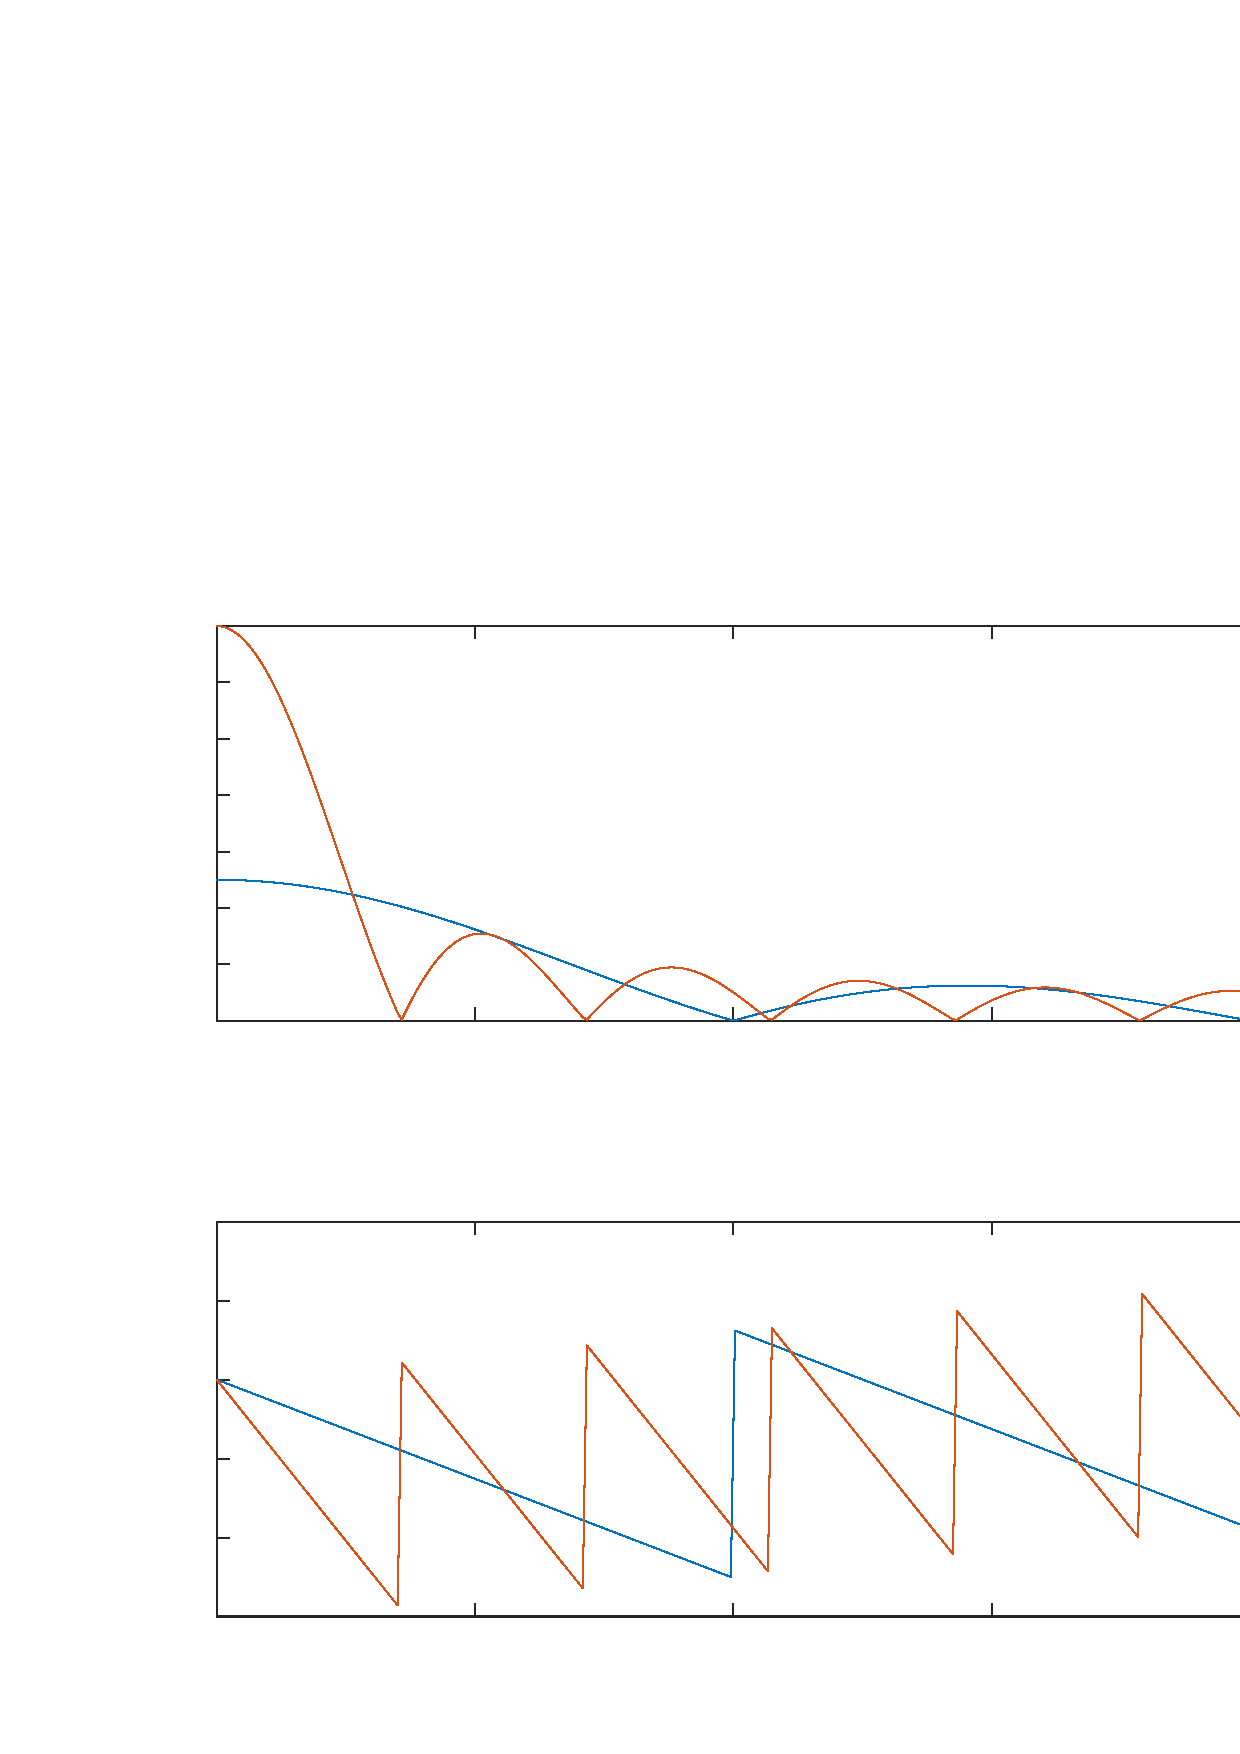
\includegraphics[scale=1]{octaves/mPointMovingAverageFilterPlot-inc}
\end{picture}%
\begin{picture}(800,600)(0,0)
\fontsize{13}{0}\selectfont\put(104,341.513){\makebox(0,0)[t]{\textcolor[rgb]{0.15,0.15,0.15}{{0}}}}
\fontsize{13}{0}\selectfont\put(228,341.513){\makebox(0,0)[t]{\textcolor[rgb]{0.15,0.15,0.15}{{0.2}}}}
\fontsize{13}{0}\selectfont\put(352,341.513){\makebox(0,0)[t]{\textcolor[rgb]{0.15,0.15,0.15}{{0.4}}}}
\fontsize{13}{0}\selectfont\put(476,341.513){\makebox(0,0)[t]{\textcolor[rgb]{0.15,0.15,0.15}{{0.6}}}}
\fontsize{13}{0}\selectfont\put(600,341.513){\makebox(0,0)[t]{\textcolor[rgb]{0.15,0.15,0.15}{{0.8}}}}
\fontsize{13}{0}\selectfont\put(724,341.513){\makebox(0,0)[t]{\textcolor[rgb]{0.15,0.15,0.15}{{1}}}}
\fontsize{13}{0}\selectfont\put(97.0647,351.944){\makebox(0,0)[r]{\textcolor[rgb]{0.15,0.15,0.15}{{0}}}}
\fontsize{13}{0}\selectfont\put(97.0647,379.015){\makebox(0,0)[r]{\textcolor[rgb]{0.15,0.15,0.15}{{2}}}}
\fontsize{13}{0}\selectfont\put(97.0647,406.086){\makebox(0,0)[r]{\textcolor[rgb]{0.15,0.15,0.15}{{4}}}}
\fontsize{13}{0}\selectfont\put(97.0647,433.158){\makebox(0,0)[r]{\textcolor[rgb]{0.15,0.15,0.15}{{6}}}}
\fontsize{13}{0}\selectfont\put(97.0647,460.229){\makebox(0,0)[r]{\textcolor[rgb]{0.15,0.15,0.15}{{8}}}}
\fontsize{13}{0}\selectfont\put(97.0647,487.301){\makebox(0,0)[r]{\textcolor[rgb]{0.15,0.15,0.15}{{10}}}}
\fontsize{13}{0}\selectfont\put(97.0647,514.372){\makebox(0,0)[r]{\textcolor[rgb]{0.15,0.15,0.15}{{12}}}}
\fontsize{13}{0}\selectfont\put(97.0647,541.444){\makebox(0,0)[r]{\textcolor[rgb]{0.15,0.15,0.15}{{14}}}}
\fontsize{15}{0}\selectfont\put(414,551.444){\makebox(0,0)[b]{\textcolor[rgb]{0,0,0}{{Magnitude response}}}}
\fontsize{12}{0}\selectfont\put(679.984,523.594){\makebox(0,0)[l]{\textcolor[rgb]{0,0,0}{{M=5}}}}
\fontsize{12}{0}\selectfont\put(679.984,507.923){\makebox(0,0)[l]{\textcolor[rgb]{0,0,0}{{M=14}}}}
\fontsize{13}{0}\selectfont\put(104,55.5695){\makebox(0,0)[t]{\textcolor[rgb]{0.15,0.15,0.15}{{0}}}}
\fontsize{13}{0}\selectfont\put(228,55.5695){\makebox(0,0)[t]{\textcolor[rgb]{0.15,0.15,0.15}{{0.2}}}}
\fontsize{13}{0}\selectfont\put(352,55.5695){\makebox(0,0)[t]{\textcolor[rgb]{0.15,0.15,0.15}{{0.4}}}}
\fontsize{13}{0}\selectfont\put(476,55.5695){\makebox(0,0)[t]{\textcolor[rgb]{0.15,0.15,0.15}{{0.6}}}}
\fontsize{13}{0}\selectfont\put(600,55.5695){\makebox(0,0)[t]{\textcolor[rgb]{0.15,0.15,0.15}{{0.8}}}}
\fontsize{13}{0}\selectfont\put(724,55.5695){\makebox(0,0)[t]{\textcolor[rgb]{0.15,0.15,0.15}{{1}}}}
\fontsize{13}{0}\selectfont\put(97.0647,66){\makebox(0,0)[r]{\textcolor[rgb]{0.15,0.15,0.15}{{-3}}}}
\fontsize{13}{0}\selectfont\put(97.0647,103.9){\makebox(0,0)[r]{\textcolor[rgb]{0.15,0.15,0.15}{{-2}}}}
\fontsize{13}{0}\selectfont\put(97.0647,141.8){\makebox(0,0)[r]{\textcolor[rgb]{0.15,0.15,0.15}{{-1}}}}
\fontsize{13}{0}\selectfont\put(97.0647,179.7){\makebox(0,0)[r]{\textcolor[rgb]{0.15,0.15,0.15}{{0}}}}
\fontsize{13}{0}\selectfont\put(97.0647,217.6){\makebox(0,0)[r]{\textcolor[rgb]{0.15,0.15,0.15}{{1}}}}
\fontsize{13}{0}\selectfont\put(97.0647,255.5){\makebox(0,0)[r]{\textcolor[rgb]{0.15,0.15,0.15}{{2}}}}
\fontsize{15}{0}\selectfont\put(414,265.5){\makebox(0,0)[b]{\textcolor[rgb]{0,0,0}{{Phase response}}}}
\fontsize{12}{0}\selectfont\put(679.984,237.651){\makebox(0,0)[l]{\textcolor[rgb]{0,0,0}{{M=5}}}}
\fontsize{12}{0}\selectfont\put(679.984,221.979){\makebox(0,0)[l]{\textcolor[rgb]{0,0,0}{{M=14}}}}
\end{picture}

}\caption{Magnitude response and phase response of an $M$-point moving average filter, with $M=5$ (blue) and $M=14$ (red).}\label{oct:mPointMovingAverageFilterPlot}
\end{center}
\end{figure*}

For instance, suppose two $M$-point moving average filters with $M=5$ and $M=14$---with the following commands
\begin{verbatim}
pkg load signal;
clear all;

h5 = [1 1 1 1 1];
h14 = [1 1 1 1 1 1 1 1 1 1 1 1 1 1];
w = [0:0.01:3.14];
[H5, W5] = freqz(h5, 1, w);
[H14, W14] = freqz(h14, 1, w);
figure(1);
subplot(2,1,1);
plot(w/3.14, abs(H5), w/3.14, abs(H14));
legend('M=5', 'M=14');
title('Magnitude response');
subplot(2,1,2);
plot(w/3.14, angle(H5), w/3.14, angle(H14));
legend('M=5', 'M=14');
title('Phase response');
\end{verbatim}
the plot in Figure~\ref{oct:mPointMovingAverageFilterPlot} is produced.

The phase response of a discrete-time system, when determined by a calculator, might exhibit sudden jumps by an amount of $2\pi$ that are caused by the way the \texttt{arctan} function is computed by only taking in account the principal value of the phase~(\ref{eqn:phasePrincipalValue}. The phase response can be accordingly ``unwrapped'', making it a continuous function of $\omega$. An example of this had been illustrated in Figure~\ref{oct:octaveExampleFreqzUnwrap}. To this end, the function \texttt{unwrap} should be employed with the phase in radians. Be careful, though: the jumps of $2\pi$ must not be confused with the jumps induced by the zeros of the frequency response, as indicated in the phase response of the moving average filter.

\section{Steady-State Response and Transient Response}
From the frequency response we are also able to determine the \emph{steady-state response} of an LTI discrete-time system to a sinusoidal input.
Let $y[n]$ be the output of a real coefficient LTI discrete-time system, with a frequency response $H(e^{j\omega})$ for a sinusoidal input of the form
\[
    x[n] = A\cos{(\omega_0 n + \varphi)}, -\infty < n < \infty;
\]
we can express the input $x[n]$ in polar representation as
\begin{align*}
    x[n] &= \frac 1 2 Ae^{j\varphi}e^{j\omega_0 n} + \frac 1 2 e^{-j\varphi}e^{-j\omega_0 n}\\
         &= g[n] + g^*[n]
\end{align*}
with $g[n] = e^{j\varphi}e^{j\omega_0n}$. Since the output of the system for an eigenfunction $e^{j\omega_0n}$ is the frequency response multiplied by the eigenfunction, one has that the output $v[n]$ of $g[n]$ is
\[
    v[n] = \frac 1 2 H(e^{j\omega_0})Ae^{j\varphi}e^{j\omega_0n}
\]
and the output $v^*[n]$ of $g^*[n]$ is
\[
    v^*[n] = \frac 1 2 H(e^{-j\omega_0})Ae^{-j\varphi}e^{-j\omega_0n}.
\]

The complete output will be the sum of the two outputs taken alone (superposition principle),
\begin{align*}
    y[n]
    &= v[n] + v^*[n]\\
    &= \frac 1 2 H(e^{j\omega_0})Ae^{j\varphi}e^{j\omega_0n} + \frac 1 2 H(e^{-j\omega_0})Ae^{-j\varphi}e^{-j\omega_0n}\\
    &= \frac 1 2 A\left|H(e^{j\omega_0})\right|\left(e^{j\theta(\omega)}e^{j\varphi}e^{j\omega_0n} + e^{-j\theta(\omega)}e^{-j\varphi}e^{-j\omega_0n}\right)\\
    &= \frac 1 2 A\left|H(e^{j\omega_0})\right|\cos{(\omega_0n + \theta(\omega_0) + \varphi)},
\end{align*}
as 
\[
    H(e^{\pm j\omega}) = \left|H(e^{+ j\omega})\right|e^{\pm j\theta(\omega)}.
\]

The output $y[n]$ has the very same sinusoidal waveform that the input has, with two substantial differences: the first being that \emph{the amplitude is multiplied by a coefficient $\left|H(e^{j\omega_0})\right|$} that is the value of the magnitude function at $\omega = \omega_0$, the oscillation frequency of the sinusoid; second, the output has a \emph{phase lag} induced by the filter by an amount $\theta(\omega_0)$, the value of the phase function at $\omega = \omega_0$.

\section{Response to a Causal Exponential Sequence}
The above expression for the steady-state assumes that the system is \emph{initially relaxed} before application of the input sinusoid, which means that the system is under no stress right before the application of $x[n]$. This culminates in the fact that, in practical applications, exerciting a solicitation $x[n]$ to a causal LTI system usually means applying an input sequence that is \emph{right-sided}, at some starting sample index $n = n_0$; for such a generic input, an output will be soon derived.

Let's assume $x[n] = e^{j\omega n}\mu[n]$ be a right-sided signal for $n < 0$, with no loss of generality with the implied causality. By looking at the input--output relationship for an LTI discrete-time system
\[
    y[n] = \sum_{k=-\infty}^\infty h[k]x[n-k]
\]
one soon observes that the output is given by the following
\begin{align*}
    y[n] &= \left(\sum_{k=0}^n h[k] e^{j\omega(n - k)}\right) \mu[n]\\
         &=\left(\sum_{k=0}^n h[k] e^{-j\omega k}\right)e^{j\omega n} \mu[n].
\end{align*}
Let's now determine the output. For $n<0$ is, trivially, $y[n]=0$. For $n \geq 0$ one must assess the above sum,
\begin{align*}
    y[n] &= \left(\sum_{k=0}^n h[k] e^{-j\omega k}\right)e^{j\omega n} \mu[n]\\
    &= \left(\sum_{k=0}^\infty h[k] e^{-j\omega k}\right)e^{j\omega n} - \left(\sum_{k=n+1}^\infty h[k] e^{-j\omega k}\right)e^{j\omega n} \\
    &= H(e^{j\omega_0})e^{j\omega n} - \left(\sum_{k=n+1}^\infty h[k] e^{-j\omega k}\right)e^{j\omega n}.
\end{align*}

The first term on the right-hand side is the same as that obtained when the input is applied at $n=0$, to an \emph{initially relaxed system} and is called the \textbf{steady-state response}
\begin{equation}\label{eqn:steadyStateResponse}
    y_{sr}[n] = H(e^{j\omega})e^{j\omega n}.
\end{equation}
Steady state occurs after the system becomes settled and at the steady system starts working normally. Steady state response of control system is a function of input signal and it is also called as forced response.

Separately, the second term on the right-hand side is said to be the \textbf{transient response}, that is the component of the response that exists until the output settles on the steady-state response,
\begin{equation}\label{eqn:transientResponse}
    y_{tr}[n] = -\left(\sum_{k=n+1}^\infty h[k] e^{-j\omega j}\right) e^{j\omega n}
\end{equation}

In order to determine the effect of the transient response, one notices that
\begin{align*}
    |y_{tr}[n]| &= \left|\sum_{k=n+1}^\infty h[k] e^{-j\omega(k-n)}\right| \\
                &\leq \sum_{k=n+1}^\infty |h[k]| \leq \sum_{k=0}^\infty |h[k]|;
\end{align*}
this means that, for a causal stable LTI system $h[n]$ will be \emph{absolutely summable}, and the previous inequality dictates that the transient response $y_{tr}[n]$ is a bounded sequence as well, inferior in module than the absolute sum of $h[k]$. In addition, transient response contribution to the output will decay over $n$; surely, as $n \rightarrow \infty$, one has that the magnitude of the transient response collapses to zero,
\[
    |y_{tr}[n]| \leq \sum_{k=n+1}^\infty |h[k]| \rightarrow 0
\]
as $n$ becomes large enough.

Finite Impulse Response LTI systems as in~\ref{eqn:finiteImpulseResponse} with an impulse response of length $N+1$, will be such that $h[n] = 0, \forall n > N$, and will as a consequence yield a \emph{null transient response} for any time sample $n > N - 1$. The output reaches the steady-state value $y_{sr}[n] = H(e^{j\omega})e^{j\omega n}$ at exactly the time sample $n = N$.

Summing up, the response to a causal exponential sequence will be the superposition of two distinct, components: a first one, being the \emph{steady-state response}, that measures the behavior of the system after a long time, when steady conditions have been reached after an external excitation, and a second one being the \emph{transient response} that takes in account the response against a temporary change in the way that the system behaves due to an external excitation, that will disappear over time. The first one will be persistent, the second will see its effect decay as $n$ increases. Both terms constitute the response of a system to a certain solicitation.

\section{The concept of Filtering}

In signal processing, a filter is a device or process that removes some unwanted components or features from a signal. Filtering is a class of signal processing, the defining feature of filters being the complete or partial suppression of some aspect of the signal. Most often, this means removing some frequencies or frequency bands. However, filters do not exclusively act in the frequency domain; especially in the field of image processing many other targets for filtering exist. Correlations can be removed for certain frequency components and not for others without having to act in the frequency domain. Filters are widely used in electronics and telecommunication, in radio, television, audio recording, radar, control systems, music synthesis, image processing, and computer graphics\cite{bib:filtering}.

One application of an LTI discrete-time system is to \emph{pass} certain frequency components in an input sequence without any distortion---if possible---and to \emph{block} unwanted frequency components. Such systems are called \textbf{digital filters}.

The key to the filtering process is represented by the following integral,
\begin{equation}\label{eqn:filteringProcess}
    x[n] = \frac 1 {2\pi} \int_{-\pi}^\pi X(e^{j\omega})e^{j\omega n}d\omega,
\end{equation}
which expresses an arbitrary input as a linear weighted sum of an infinite number of exponential sequences---or equivalently as a \emph{linear weighted sum of sinusoidal sequences}, whose weights are the values of the Discrete-time Fourier Transform $X(e^{j\omega})$. The filtering process occurs by carefully choosing the function $X$ (that will be the frequency response $H(e^{j\omega})$ of an LTI digital filter) so that its magnitude $\left|H(e^{j\omega})\right|$ is greater or lower at some frequencies depending on the needs. Since any input sinusoid will be multiplied by the magnitude of the frequency response of the filter, then one can \emph{amplify} or \emph{attenuate} some frequency at will by designing a suitable frequency response.

\subsection{Core concepts behind filters}

To better understand the inner workings behind the design of filters that are actually able to filter specific frequencies, consider a real-coefficient LTI discrete-time system characterized by
\begin{equation}\label{exa:idealFilter1}
    \left|H(e^{j\omega})\right| \cong
    \left\{
        \begin{array}{ll}
            1 & |\omega| \leq \omega_c\\
            0 & \omega_c < |\omega| \leq \pi
        \end{array}
    \right..
\end{equation}

We then apply to the above system an input composed of sinusoids
\[
    x[n] = A\cos{\omega_1 n} + B\cos{\omega_2 n}
\]
at two, distinct, frequencies $\omega_1$ and $\omega_2$, so that $0 < \omega_1 < \omega_c < \omega_2 < \pi$.

Due to linearity, the outputs of this system will be the superposition of the two responses to the single sinusoids of distinct frequencies:
\begin{align*}
    y[n] &=
        A\left|H(e^{j\omega_1})\right|\cos{(\omega_1 n + \theta(\omega_1))} \\
        &+ B\left|H(e^{j\omega_2})\right|\cos{(\omega_2 n + \theta(\omega_2))},
\end{align*}
and please notice that, in this case, initial phases $\varphi_1 = 0$ and $\varphi_2=0$.

Now, from the definition~\ref{exa:idealFilter1} of the filter it results that
\begin{align*}
    \left|H(e^{j\omega_1})\right| \simeq 1 &  & \left|H(e^{j\omega_2})\right| \simeq 0,
\end{align*}
the output will reduce to
\begin{align*}
    y[n] &=
        A\left|H(e^{j\omega_1})\right|\cos{(\omega_1 n + \theta(\omega_1))} \\
        &+ B\left|H(e^{j\omega_2})\right|\cos{(\omega_2 n + \theta(\omega_2))},\\
    y[n] &\simeq
        A\left|H(e^{j\omega_1})\right|\cos{(\omega_1 n + \theta(\omega_1))}
\end{align*}
as the term corresponding to frequency $\omega_2$ \emph{has been filtered} since $\left|H(e^{j\omega_2})\right| \simeq 0$. Term corresponding to frequency $\omega_1$, instead, is allowed to simply pass---the value of the frequency response at frequency $\omega_1$ is close to $1$. A simple illustration of the filter is depicted just below,
\begin{center}
    \begin{tikzpicture}
        \draw[-stealth, thick] (-1, 0) -- (3.5, 0) node[anchor=west] {$\omega$};
        \draw[-stealth, thick] (0, -.5) -- (0, 2) node[anchor=south west] {$\left|H(e^{j\omega})\right|$};
        \draw[thick] (0, 1) node[anchor=east] {$1$} -- (1.7, 1) -- (1.7, 0) node[anchor=north] {$\omega_c$};
        \draw (2.8, +1mm) -- (2.8, -1mm) node[anchor=north west] {$\pi$};
        \draw [-stealth, green, thick] (.85, 0) -- (.85, 1.2) node[anchor=south] {$\omega_1$};
        \draw [-stealth, red, thick] (2.15, 0) -- (2.15, 1.2) node[anchor=south] {$\omega_2$};
    \end{tikzpicture}
\end{center}
where the green sinusoid is allowed to pass, the red sinusoid is instead filtered out (multiplied by a value that is very close to---if not exactly---zero).

In virtue of the fact that only frequencies lower than a certain frequency $\omega_c$ are allowed to pass, the system is called a \textbf{lowpass filter}. Conversely, filters that allow to pass frequencies higher than a certain frequency $\omega_c$ are called \textbf{highpass filters}. Furthermore, we say that a filter is a \textbf{bandpass filter} when the range of frequencies allowed to pass is between two values $\omega_h$ and $\omega_l$, that is a digital filter that favors the passage of frequencies $\omega_l < \omega < \omega_h$.

Suppose the input $x[n]$ of a digital filter we have to design consists of a sum of two distinct sinusoidal sequences $a[n]$ and $b[n]$ of angular frequencies $0.1 \mbox{rad/sample}$ and $0.4 \mbox{rad/sample}$, and the goal is to design a highpass filter to block the low-frequency component spinning at $0.1$ radians for sample. For simplicity, let's assume the filter to be a FIR filter of length $3$, with an impulse response of 
\[
    \{h[n]\} = \{\alpha, \beta, \alpha\}
\]
that is $h[0] = h[2] = \alpha$ and $h[1] = \beta$. In order to determine the output $y[n]$ a convolution sum has to be performed:
\begin{align*}
    y[n] 
    &= h[0]x[n] + h[1]x[n-1] + h[2]x[n-2]\\
    &= \alpha x[n] + \beta x[n-1] + \alpha x[n-2].
\end{align*}

It is clear that adequate values of $\alpha$ and $\beta$ should be chosen for only the higher sinusoid to pass. To do so, one has to look at the frequency response of the FIR filter:
\begin{align*}
    H(e^{j\omega})
        &= h[0] + h[1]e^{-j\omega} + h[2]e^{-j2\omega}\\
        &= \alpha + \alpha e^{-j2\omega} + \beta e^{-j\omega}\\
        &= \alpha (1 + e^{-j2\omega}) + \beta e^{-j\omega}\\
        &= 2\alpha \left(\frac{e^{j\omega} + e^{-j\omega}}{2}\right)e^{-j\omega} + \beta e^{-j\omega}\\
        &= (2\alpha \cos{\omega} + \beta) e^{-j\omega},
\end{align*}
whose magnitude and phase functions are 
\begin{align*}
    \left|H(e^{j\omega})\right| &= 2 \alpha \cos\omega + \beta,\\
    \theta(\omega) &= -\omega.
\end{align*}

For the magnitude function to block the low-frequency component it has to be equal or very close to $0$ in $\omega=0.1$; on contrary, for $\omega=0.4$ to successfully pass the magnitude function should be equal---or very close to---one. But this is equivalent to solve the following systems of equations
\[
\left\{
    \begin{array}{ll}
        \left|H(e^{j0.1})\right| =& 2\alpha \cos{(0.1)} + \beta = 0\\
        \left|H(e^{j0.4})\right| =& 2\alpha \cos{(0.4)} + \beta = 0
    \end{array}
\right.,
\]
that can be solved by a computer; it yields
\begin{align*}
    \alpha &= -6.76195\\
    \beta  &= 13.456335,
\end{align*}
and in the end the input--output relationship of the FIR filter in exam is
\[
    y[n] = -6.76195(x[n] + x[n-2]) + 13.456335x[n-2]
\]
for an input of $x[n] = \{\cos{(0.1n)} + \cos{(0.4n)}\}\mu[n]$.

\begin{figure*}[ht]
\begin{center}
\scalebox{0.6}{
    % Title: gl2ps_renderer figure
% Creator: GL2PS 1.4.2, (C) 1999-2020 C. Geuzaine
% For: Octave
% CreationDate: Thu Nov 10 14:39:43 2022
\setlength{\unitlength}{1pt}
\begin{picture}(0,0)
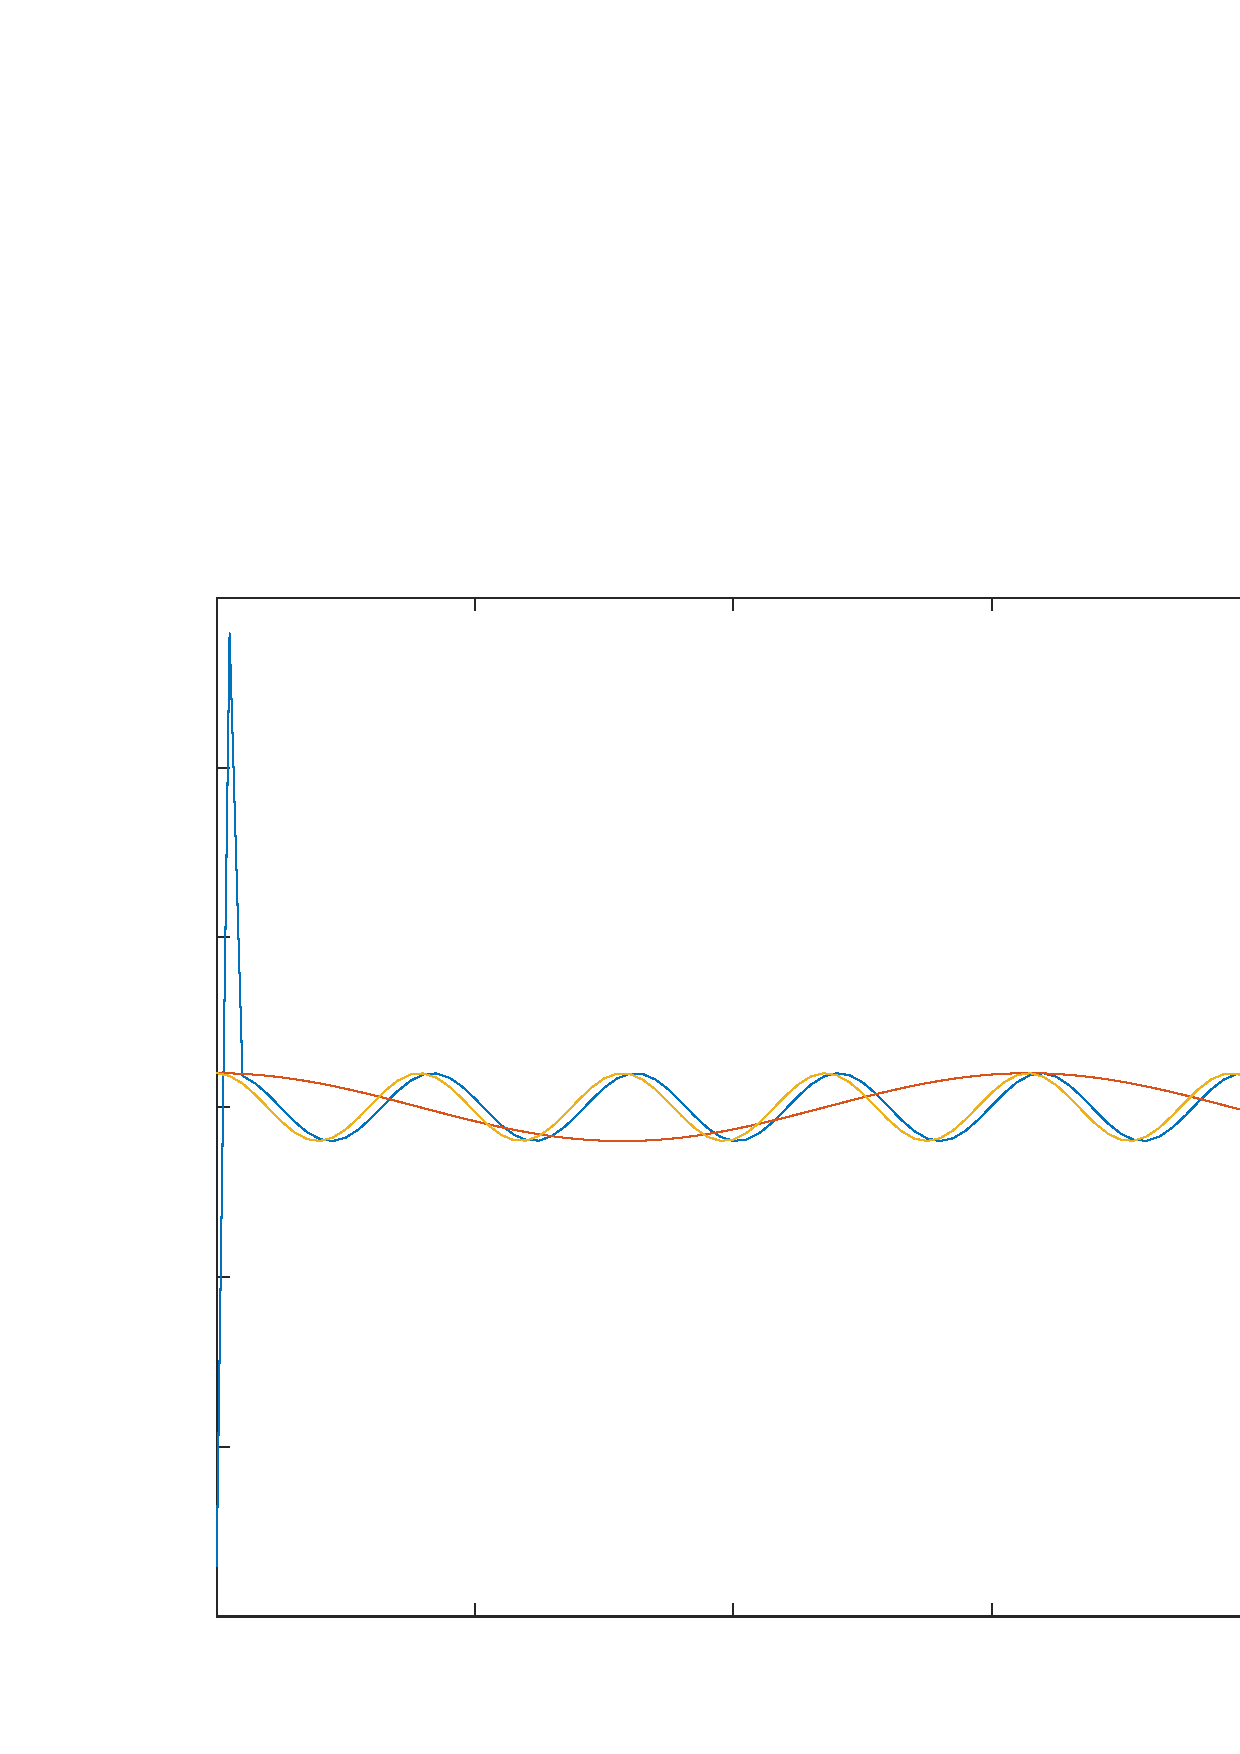
\includegraphics[scale=1]{octaves/highpassFilterExample1-inc}
\end{picture}%
\begin{picture}(800,600)(0,0)
\fontsize{13}{0}\selectfont\put(104,55.597){\makebox(0,0)[t]{\textcolor[rgb]{0.15,0.15,0.15}{{0}}}}
\fontsize{13}{0}\selectfont\put(228,55.597){\makebox(0,0)[t]{\textcolor[rgb]{0.15,0.15,0.15}{{20}}}}
\fontsize{13}{0}\selectfont\put(352,55.597){\makebox(0,0)[t]{\textcolor[rgb]{0.15,0.15,0.15}{{40}}}}
\fontsize{13}{0}\selectfont\put(476,55.597){\makebox(0,0)[t]{\textcolor[rgb]{0.15,0.15,0.15}{{60}}}}
\fontsize{13}{0}\selectfont\put(600,55.597){\makebox(0,0)[t]{\textcolor[rgb]{0.15,0.15,0.15}{{80}}}}
\fontsize{13}{0}\selectfont\put(724,55.597){\makebox(0,0)[t]{\textcolor[rgb]{0.15,0.15,0.15}{{100}}}}
\fontsize{13}{0}\selectfont\put(97.0647,66){\makebox(0,0)[r]{\textcolor[rgb]{0.15,0.15,0.15}{{-15}}}}
\fontsize{13}{0}\selectfont\put(97.0647,147.5){\makebox(0,0)[r]{\textcolor[rgb]{0.15,0.15,0.15}{{-10}}}}
\fontsize{13}{0}\selectfont\put(97.0647,229){\makebox(0,0)[r]{\textcolor[rgb]{0.15,0.15,0.15}{{-5}}}}
\fontsize{13}{0}\selectfont\put(97.0647,310.5){\makebox(0,0)[r]{\textcolor[rgb]{0.15,0.15,0.15}{{0}}}}
\fontsize{13}{0}\selectfont\put(97.0647,392){\makebox(0,0)[r]{\textcolor[rgb]{0.15,0.15,0.15}{{5}}}}
\fontsize{13}{0}\selectfont\put(97.0647,473.5){\makebox(0,0)[r]{\textcolor[rgb]{0.15,0.15,0.15}{{10}}}}
\fontsize{13}{0}\selectfont\put(97.0647,555){\makebox(0,0)[r]{\textcolor[rgb]{0.15,0.15,0.15}{{15}}}}
\fontsize{12}{0}\selectfont\put(691.984,536.484){\makebox(0,0)[l]{\textcolor[rgb]{0,0,0}{{y[n]}}}}
\fontsize{12}{0}\selectfont\put(691.984,519.479){\makebox(0,0)[l]{\textcolor[rgb]{0,0,0}{{a[n]}}}}
\fontsize{12}{0}\selectfont\put(691.984,502.474){\makebox(0,0)[l]{\textcolor[rgb]{0,0,0}{{b[n]}}}}
\end{picture}

}\caption{Response to the highpass filter in the previous example. As one can see, the sinusoid with the lowest frequency is successfully discarded. The output presents a huge peak at the beginning and a persistent phase delay after, though, that is due to the nature of the filtering technique.}\label{oct:highpassFilterExample1}
\end{center}
\end{figure*}

\begin{figure*}[ht]
\begin{center}
\scalebox{0.6}{
    % Title: gl2ps_renderer figure
% Creator: GL2PS 1.4.2, (C) 1999-2020 C. Geuzaine
% For: Octave
% CreationDate: Fri Nov 11 15:24:43 2022
\setlength{\unitlength}{1pt}
\begin{picture}(0,0)
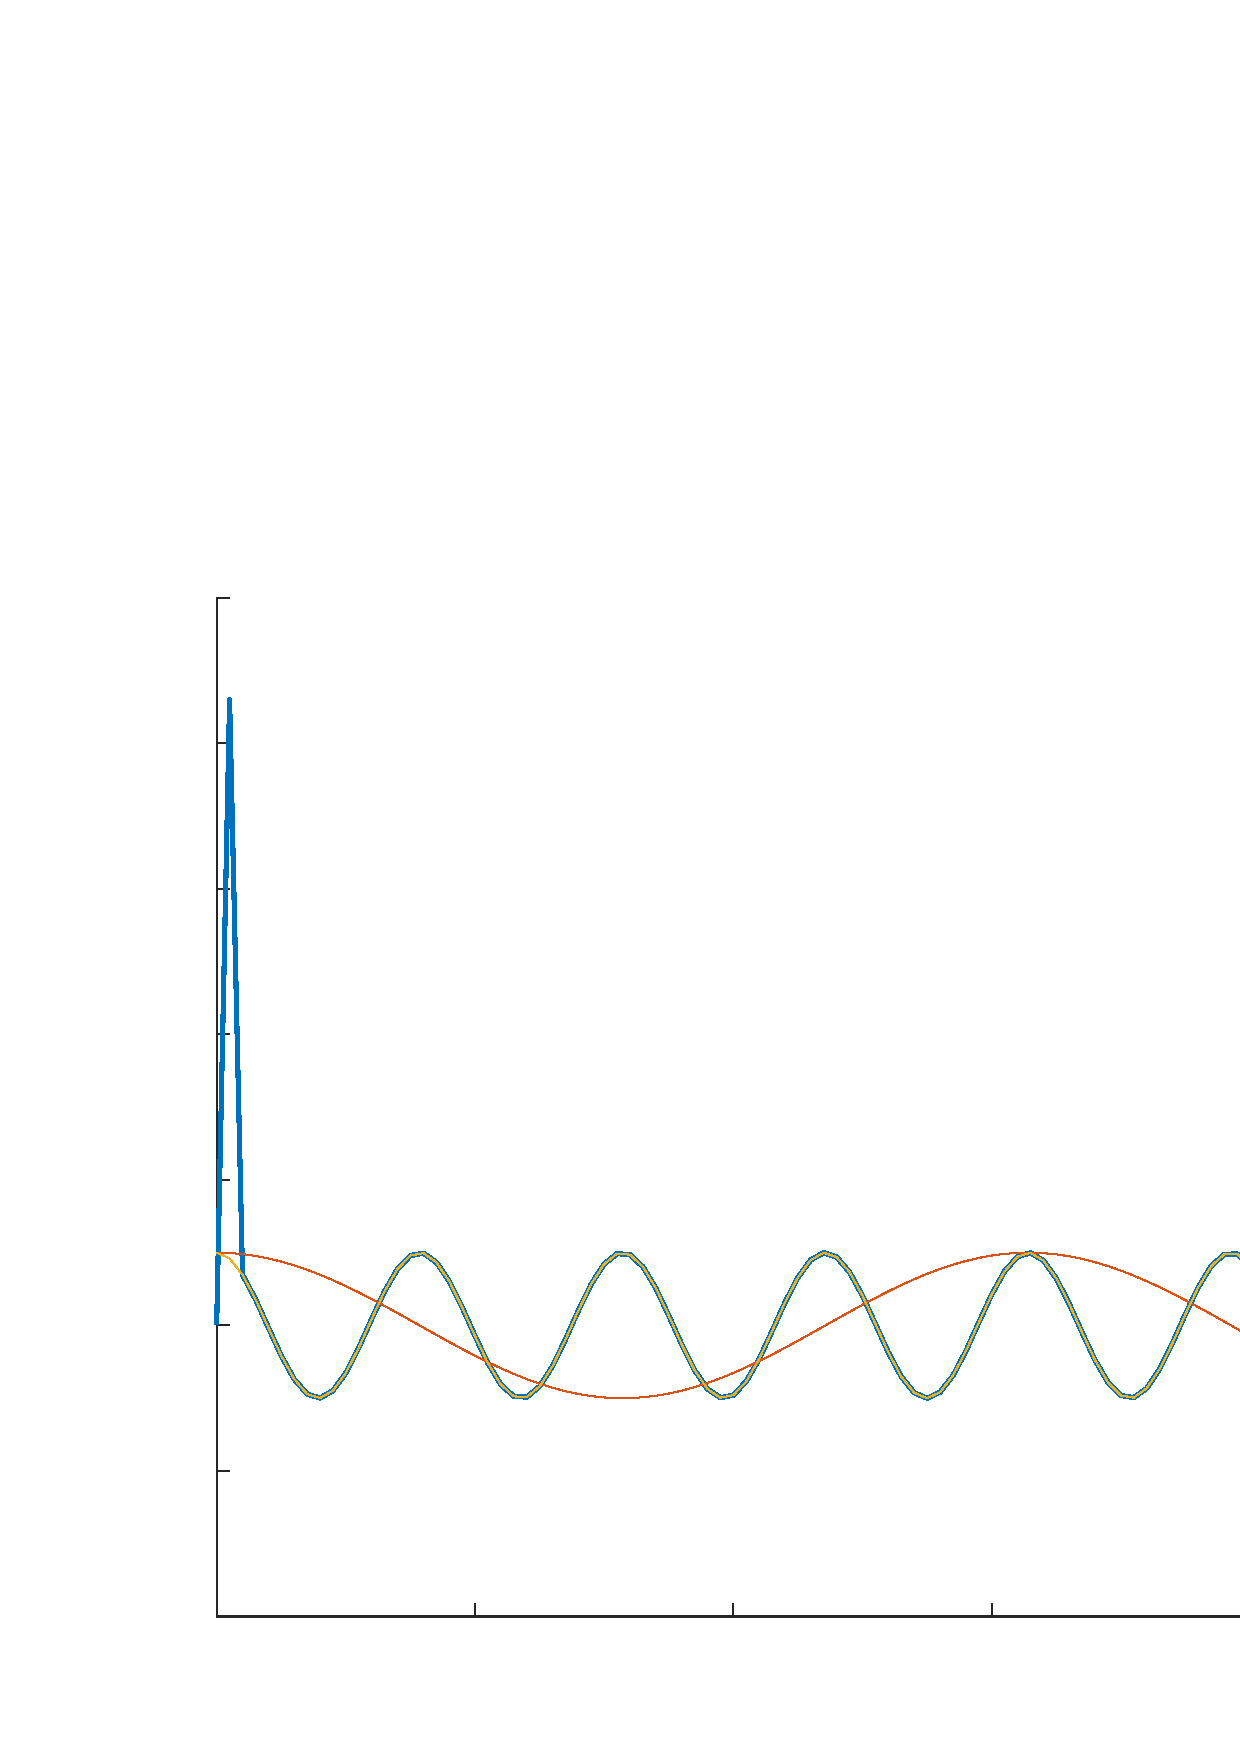
\includegraphics[scale=1]{octaves/highpassFilterExample2-inc}
\end{picture}%
\begin{picture}(800,600)(0,0)
\fontsize{13}{0}\selectfont\put(104,55.597){\makebox(0,0)[t]{\textcolor[rgb]{0.15,0.15,0.15}{{0}}}}
\fontsize{13}{0}\selectfont\put(228,55.597){\makebox(0,0)[t]{\textcolor[rgb]{0.15,0.15,0.15}{{20}}}}
\fontsize{13}{0}\selectfont\put(352,55.597){\makebox(0,0)[t]{\textcolor[rgb]{0.15,0.15,0.15}{{40}}}}
\fontsize{13}{0}\selectfont\put(476,55.597){\makebox(0,0)[t]{\textcolor[rgb]{0.15,0.15,0.15}{{60}}}}
\fontsize{13}{0}\selectfont\put(600,55.597){\makebox(0,0)[t]{\textcolor[rgb]{0.15,0.15,0.15}{{80}}}}
\fontsize{13}{0}\selectfont\put(724,55.597){\makebox(0,0)[t]{\textcolor[rgb]{0.15,0.15,0.15}{{100}}}}
\fontsize{13}{0}\selectfont\put(97.0647,66){\makebox(0,0)[r]{\textcolor[rgb]{0.15,0.15,0.15}{{-4}}}}
\fontsize{13}{0}\selectfont\put(97.0647,135.857){\makebox(0,0)[r]{\textcolor[rgb]{0.15,0.15,0.15}{{-2}}}}
\fontsize{13}{0}\selectfont\put(97.0647,205.714){\makebox(0,0)[r]{\textcolor[rgb]{0.15,0.15,0.15}{{0}}}}
\fontsize{13}{0}\selectfont\put(97.0647,275.571){\makebox(0,0)[r]{\textcolor[rgb]{0.15,0.15,0.15}{{2}}}}
\fontsize{13}{0}\selectfont\put(97.0647,345.429){\makebox(0,0)[r]{\textcolor[rgb]{0.15,0.15,0.15}{{4}}}}
\fontsize{13}{0}\selectfont\put(97.0647,415.286){\makebox(0,0)[r]{\textcolor[rgb]{0.15,0.15,0.15}{{6}}}}
\fontsize{13}{0}\selectfont\put(97.0647,485.143){\makebox(0,0)[r]{\textcolor[rgb]{0.15,0.15,0.15}{{8}}}}
\fontsize{13}{0}\selectfont\put(97.0647,555){\makebox(0,0)[r]{\textcolor[rgb]{0.15,0.15,0.15}{{10}}}}
\fontsize{12}{0}\selectfont\put(691.984,536.484){\makebox(0,0)[l]{\textcolor[rgb]{0,0,0}{{y[n]}}}}
\fontsize{12}{0}\selectfont\put(691.984,519.479){\makebox(0,0)[l]{\textcolor[rgb]{0,0,0}{{a[n]}}}}
\fontsize{12}{0}\selectfont\put(691.984,502.474){\makebox(0,0)[l]{\textcolor[rgb]{0,0,0}{{b[n]}}}}
\end{picture}

}\caption{Response to the highpass filter in the previous example, but with a zero phase delay filter. This is achieved by means of function \texttt{filtfilt}, which grants a filter whose output does not suffer a phase delay at all. The price to pay is a small artifact at the end of the filtering phase; moreover, this has a different frequency response that the one that one had at the beginning, and is possible only with a relatively short sequence so that we can pass it twice through the system, before and after flipping it: this is only feasible if one is not operating in real-time applications. Formally, this will be tackled later on in the book.}\label{oct:highpassFilterExample2}
\end{center}
\end{figure*}

As it can be witnessed by Figure~\ref{oct:highpassFilterExample1}, there is a huge peak at the very beginning of the output sequence---the sudden bounce in values is given by the fact that the first starts from $0$ and has to first be \emph{charged} by obtaining proper values for $x[n]$, $x[n-1]$ and $x[n-2]$. Only after collecting all required input values for the formula
\[
    y[n] = -6.76195(x[n] + x[n-2]) + 13.456335x[n-2]
\]
one can properly compute the output value and obtain a proper filtering action. The first two samples of $y[n]$ are, in fact, the result of a filter that assumed $x[n-1]$ and $x[n-2]$ to be $0$. For this reason, the first two output samples constituite the \emph{transient} part of the output, while the \emph{steady-state} is reached at $n = N = 2$, as the impulse response has length $N + 1 = 3$. The output is a delayed version of one sample period of the high-frequency component $b[n] = \cos{(0.4n)}$ of the input.

\subsection{Phase delay}

If an input $x[n]$ to an LTI system $H(e^{j\omega})$ is a sinusoidal signal of frequency $\omega_0$, such as
\[
    x[n] = A\cos{(\omega_0 n + \varphi)}, -\infty < n < \infty,
\]
then the output $y[n]$ will be also a sinusoidal sequence of the very same frequency $\omega_0$, but lagging in phase of quantity $\theta(\omega_0)$ radians, the \emph{phase response}, since we have seen that the output sequence formula is determined by
\[
    y[n] = A\left|H(e^{j\omega_0})\right| \cos{(\omega_0 n +\theta(\omega_0) + \varphi)}, -\infty < n < \infty.
\]
Indeed, the phase delay manifests as an additive term in the argument of the sinusoidal output function, and is characterized by the frequency response of the filter $H(e^{j\omega})$, in particular it coincides to the phase response of the frequency response.

The output expression can be soon rewritten as
\begin{equation}\label{eqn:phaseDelayResponse}
    y[n] = A\left|H(e^{j\omega_0})\right|\cos{\left(\omega_0\left(n - \tau_p(\omega_0)\right) + \varphi\right)}
\end{equation}
where the term
\begin{equation}\label{eqn:phaseDelay}
    \tau_p(\omega_0) :=
    -\frac {
        \theta(\omega_0)
    } {
        \omega_0
    }
\end{equation}
is called the \textbf{phase delay} of the filter whose frequency response is $H(e^{j\omega})$. The phase delay is the phase response of the filter $H$ \emph{normalized} by the frequency at which it applies $\omega_0$. The two minus signs in the two equations may confuse at first; however, it is clear that if we define the lag as a time delay $n - \tau_p(\omega_0)$ one has to define the phase delay with a minus sign as well, in order for the argument of the cosine to be subject to an actual delay. Substituting the phase delay equation~\ref{eqn:phaseDelay} in the above equation~\ref{eqn:phaseDelayResponse} one obtains the output response as already known.

Therefore, the output $y[n]$ is a time-delayed version of the input $x[n]$ of frequency $\omega_0$, with delay $\tau_p(\omega_0) =
    -\frac {
        \theta(\omega_0)
    } {
        \omega_0
    }$.
Generally speaking, the output sequence will not be a delayed replica of the input sequence, unless the phase delay $\tau_p(\omega_0)$ is actually an integer---phase delay has a physical meaning only with respect to the underlying continuous-time functions associated with $y[n]$ and $x[n]$---if the phase delay is not an integer then the output will be \emph{different} from the input, not being an exact \emph{delayed replica} of the input signal, but will instead be different, while still preserving the same shape. In nearly all cases $\tau_p(\omega_0) \in \mathbb{Q}$ is not an integer: this means that practically the output function will be the same function, but computed at non-integer samples.

\subsection{Group delay}

When the input is composed of many sinusoidal components, each one with different frequencies that are not harmonically related, each component will go through different phase delays as their phase delay term $-\frac{\theta(\omega_0)}{\omega_0}$ will have a different value. In this case, the signal delay is determined by the \textbf{group delay} quantity
\begin{equation}\label{eqn:groupDelay}
    \tau_g(\omega) = - \frac{
        d\theta(\omega)
    } {
        d\omega
    }.
\end{equation}

In defining group delay, it is assumed that the phase function is unwrapped so that its derivatives exist---otherwise, computation woul be impossible. Group delay also possesses a physical meaning only with respect to the underlying continuous time functions associated with $y[n]$ and $x[n]$: if the phase delay function $\tau_p(\omega)$ is a function of the ratio between $\theta(\omega)$ and $\omega$ that varies across $\omega$ space, the group delay is the negative derivative of $\theta(\omega)$, hence it is the tangent of the phase delay function $\tau_p(\omega)$.

Usually, we are interested in both phase delay and group delay, but the latter specially can help us determine how the \emph{delay of the waveform} behaves from the input to the output.

For instance, let's consider the phase function of the FIR filter
\[
    y[n] = \alpha x[n] + \beta x[n-1] + \alpha x[n-2]
\]
as the previous example, which is $\theta(\omega) = -\omega$. Hence, its group delay is given by
\[
    \tau_g(\omega) = +1,
\]
verifying the result of Figure~\ref{oct:highpassFilterExample1}. In this specific, case the phase delay and the group delay coincide, except for the sign.

Let now 
\[
    h[n] = 
    \left\{
        \begin{array}{ll}
            \frac 1 M & 0 \leq n \leq M-1\\
            0 & \mbox{ otherwise}
        \end{array}
    \right.
\]
be an $M$-point moving average FIR filter. Its phase function is
\begin{equation}\label{eqn:mPointMovingAverageFilterPhaseFunction}
    \theta(\omega) = -\frac{(M-1)\omega}{2} + \pi\sum_{k=0}^{\frac M 2} \mu\left(\omega - \frac {2 \pi k}{M}\right),
\end{equation}
a linear phase system. Its group delay is the negative derivative of the above (divided by $\omega$),
\begin{equation}\label{eqn:mPointMovingAverageFilterGroupDelay}
    \tau_g(\omega) = \frac {M-1}{2}.
\end{equation}

The term in the sum of~\ref{eqn:mPointMovingAverageFilterPhaseFunction} should vanish as it only represents the sudden jumps every $2\pi$ the phase is subject to; although considering them would provide a more accurate mathematical representation, they can be discarded as they add little meaning and effect to the group delay representation. Even in this case, the phase delay and the group delay coincide, except for the sign.

The physical significance of the phase and group delay are better understood by examining the continuous-time case.

Consider, in fact, an LTI continuous-time system with a frequency response of 
\[
    H_a(j\omega) = \left|H_a(j\omega)\right|e^{j\theta_a(\omega)}
\]
excited by a narrow-band amplitude modulated continuous-time signal
\[
    x_a(t) = a(t) \cos{(\omega_c t)},
\]
with $a(t)$ being a lowpass modulating signal with a band-limited Continuous-time Fourier Transform given by the following
\begin{align*}
    \left|A(j\omega)\right| = 0 & &|\omega| > \omega_0
\end{align*}
with $\cos{(\omega_c t)}$ being the \emph{high-frequency carrier signal}.

We assume that in the frequency range $\omega_c - \omega_0 < |\omega| < \omega_c + \omega_0$ the frequency response of the continuous-time system has a constant magnitude and a linear phase, that is
\begin{align*}
    \left|H_a(j\omega)\right| &= \left|H_a(j\omega_c)\right|\\
    \theta_a(\omega) &= \theta_a(\omega_c) - (\omega - \omega_c)\frac{d\theta_a(\omega)}{d\omega}\Bigr\rvert_{\omega=\omega_c}\\
                     &= -\omega_c \tau_p(\omega_c) + (\omega - \omega_c)\tau_g(\omega_c).
\end{align*}

The Continuous-time Fourier Transform of $x_a(t)$ is given by
\[
    X_a(j\omega) = \frac 1 2\left(A(j(\omega + \omega_c)) + A(j(\omega - \omega_c))\right);
\]
because of the band-limiting constraint $X_a(j\omega) = 0$ outside of the above specified frequency range $\omega_c - \omega_0 < |\omega| < \omega_c + \omega_0$. Resulting output response $y_a(t)$ of the LTI continuous-time system is given by
\[
    y_a(t) = a(t - \tau_g(\omega_c))\cos{\left(\omega_c(t - \tau_p(\omega_c))\right)},
\]
assuming $\left|H_a(j\omega_c)\right| = 1$.

What happens is that in the continuous-time case the \emph{group delay} $\tau_g(\omega_c)$ is exactly the \emph{delay that characterizes the envelope} $a(t)$ of the input signal $x_a(t)$, whilst the \emph{phase delay} $\tau_p(\omega_c)$ is the \emph{delay of the carrier}. Therefore, group delay modifies the envelope signal, while phase delay alters the carrier. This can be seen in Figure~\ref{tikz:groupDelayPlot}, where a function has been plotted in both its original form and delayed version.

\begin{figure*}[ht]
\begin{center}
    \begin{tikzpicture}[
        ]
            \begin{axis}[
                at={(0,0)},
                %xlabel = $\frac \omega \pi$,
                % ytick = {0,0.2,0.4,0.6,0.8,1},
                %yticklabels = {$0.2$,$0.4$,$0.6$,$0.8$,$1$},
                %xtick = {0,0.2,0.4,0.6,0.8,1},
                %xticklabels = {$0$,$0.2$,$0.4$,$0.6$,$0.8$,$1$},
                %ytick = {1},
                %yticklabels = {1},
                domain = 0:1,
                samples = 200,
                legend style = {%
                at = {(0.5,1.02)},
                anchor = south},
                ]
                \addlegendentry{Non delayed signal}
                        \addplot[mark = none, thick] gnuplot[raw gnuplot] {
                            a(x) = 5*x*exp(-1.5*x);
                            c(x) = cos(2*pi*x);
                            y(x) = a(x)*c(x);
                            plot[+0:6] y(x);
                    };
                        \addplot+[mark = none, draw=black, dashed, thick] gnuplot[raw gnuplot] {
                            a(x) = 5*x*exp(-1.5*x);
                            plot[+0:6] a(x);
                    };
                        \addplot+[mark = none, draw=black, dashed, thick] gnuplot[raw gnuplot] {
                            a(x) = 5*x*exp(-1.5*x);
                            plot[+0:6] -a(x);
                    };
            \end{axis};
    \end{tikzpicture}
    \begin{tikzpicture}[
        ]
            \begin{axis}[
                at={(0,0)},
                %xlabel = $\frac \omega \pi$,
                % ytick = {0,0.2,0.4,0.6,0.8,1},
                %yticklabels = {$0.2$,$0.4$,$0.6$,$0.8$,$1$},
                %xtick = {0,0.2,0.4,0.6,0.8,1},
                %xticklabels = {$0$,$0.2$,$0.4$,$0.6$,$0.8$,$1$},
                %ytick = {1},
                %yticklabels = {1},
                domain = 0:1,
                samples = 200,
                legend style = {%
                at = {(0.5,1.02)},
                anchor = south},
                ]
                \addlegendentry{Group delayed signal}
                        \addplot[mark = none, draw=black, thick] gnuplot[raw gnuplot] {
                            a(x) = 5*x*exp(-1.5*x);
                            c(x) = cos(2*pi*x);
                            y(x) = a(x)*c(x);
                            z(x) = 0;
                            plot[+0:1] z(x);
                            plot[+1:6] y(x-1);
                    };
                        \addplot+[mark = none, draw=black, dashed, thick] gnuplot[raw gnuplot] {
                            a(x) = 5*x*exp(-1.5*x);
                            plot[+1:6] a(x-1);
                    };
                        \addplot+[mark = none, draw=black, dashed, thick] gnuplot[raw gnuplot] {
                            a(x) = 5*x*exp(-1.5*x);
                            plot[+1:6] -a(x-1);
                    };
            \end{axis};
            \node at (1,2.4) {$\tau_g$};
            \draw [stealth-stealth] (.6, 2.6) -- (1.4, 2.6);
    \end{tikzpicture}
\end{center}\caption{Plots of original signal $a(t)\cos{2\pi t}$, with $a(t) = 5te^{-1.5t}$, and group delayed signals $a(t-\tau_g)\cos{2\pi (t-\tau_p)}$. The envelope is affected by the group delay, while the carrier is insterested by the phase delay. The \emph{overall profile} will be delayed by group delay $\tau_g$, while the carrier only will be delayed by the phase delay $\tau_p$. This is especially visible for continuous-time signals, but can also be applied for discrete-time signals.}\label{tikz:groupDelayPlot}
\end{figure*}

%In \textsc{Octave}, the phase delay can be computed by means of function \texttt{phasedelay}. For instance, suppose one has to compute the phase delay of the following
%\[
    %H(e^{j\omega}) = \frac{
        %0.1367(1 - e^{-j2\omega})
    %} {
        %1 - 0.5335 e^{-j\omega} + 0.7265 e^{-j2\omega}
    %};
%\]
%to do so, one has to first construct a proper filter,

The waveform of the underlying continuous-time output shows \emph{distortion} when the group delay is not constant over the bandwidth---this is because a signal usually has a lot of frequency components, and when each one gets filtered by an LTI system then different group delays will be applied to each frequency component. Indeed, the group delay is a function of $\omega$, generally speaking. In some circumstances, the distortion is unacceptable; an \emph{allpass delay equalizer} is usually cascaded with the LTI system, so that the overall group delay is \emph{approximately linear} over the frequency range of interest. This, of course, should be done while keeping the magnitude response of the original LTI system unmodified.

\chapter{Analysis of LTI Discrete-Time Systems in the Transform Domain}

In the \textbf{transform domain} it is trivial to deal with the analysis and with the characterization of an LTI system. Any LTI system is completely characterized by its impulse response sequence $\{h[n]\}$; as such, the transform of that sequence would grant us some additional insights into the behavior of such systems, by looking at the \emph{frequency response}. In fact, it is much easier to design filters by manipulating the frequency response instead of their impulse response. We now consider the use of the Discrete-time Fourier Transform and the $z$-transform to migrate from a time-domain representation to a frequency-domain representation and mitigate the difficulty of dealing with the former.

In this book we shall be concerned with LTI discrete-time systems (filters) that are characterized by linear constant coefficients difference equations, having form
\begin{equation}\label{eqn:ltiDiscreteTimeLinearConstantCoefficientsDifference}
    \sum_{k=0}^N d_k y[n-k] = \sum_{k=0}^M p_k x[n-k].
\end{equation}
Such filters are specified in a \emph{recursive} way, as the output $y[n]$ is determined by inputs $x[n - k]$ \emph{and} previous outputs $y[n-k]$.

Applying $z$-transform on both sides of the difference equation, along with properties of linearity and time-invariance, quickly yields
\begin{equation}\label{eqn:zTransformLtiDiscreteTimeLinearConstantCoefficientsDifference}
    \sum_{k=0}^N d_k z^{-k} Y(z) = \sum_{k=0}^M p_k z^{-k} X(z),
\end{equation}
with $X(z)$ and $Y(z)$ being the $z$-transforms of---respectively---$x[n]$ and $y[n]$ with corresponding associated RoCs that shall not be forgotten. Terms $z^{-k}$ appear due to $z$-transform properties related to time-shifting. Each of the components $y[n]$ can be transformed in $z^{-k}Y(z)$ and multiplied by the very same factor $d_k$---the same goes for $x[n]$ components.

A way more convenient representation is given by the following formula, in which some parentheses highlights the fact that the $z$-transforms have been collected,
\[
    \left(\sum_{k=0}^N d_k z^{-k}\right) Y(z) = \left(\sum_{k=0}^M p_k z^{-k}\right) X(z),
\]
which suddenly leads to
\begin{equation}\label{eqn:zTransformLtiDiscreteTimeLinearConstantCoefficientsDifferenceAlternate}
    Y(z) = \frac {
        \left(\sum_{k=0}^M p_k z^{-k}\right)
    } {
        \left(\sum_{k=0}^N d_k z^{-k}\right)
    } X(z),
\end{equation}
in which it is clear that the output $z$-transform is given by the input $z$-transform, multiplied by a ratio of polynomials $H(z) = \frac{D(z)}{P(z)}$ that, certainly, is the \emph{transfer function} of the system.

To prove it, let's consider the output as given by the convolution sum
\[
    y[n] = \sum_{k=-\infty}^\infty h[k] x[n-k]
\]
and move it into the frequency-domain by applying the $z$-transform to it. Applying $z$-transform rules,
\begin{align*}
    Y(z) 
    &= \sum_{n=-\infty}^\infty y[n]z^{-n} \\
    &= \sum_{n=-\infty}^\infty \left(\sum_{k=-\infty}^\infty h[k] x[n-k]\right)z^{-n}\\
    &= \sum_{k=-\infty}^\infty h[k] \left(\sum_{n=-\infty}^\infty x[n-k]z^{-n}\right)\\
\end{align*}
\begin{align*}
    &= \sum_{k=-\infty}^\infty h[k] \left(\sum_{l=-\infty}^\infty x[l]z^{-(l+k)}\right)\\
    &= \sum_{k=-\infty}^\infty h[k] \underbrace{\left(\sum_{l=-\infty}^\infty x[l]z^{-l}\right)}_{X(z)}z^{-k}\\
    &= \underbrace{\left(\sum_{k=-\infty}^\infty h[k]z^{-k}\right)}_{H(z)} X(z)\\
    &= H(z)X(z)
\end{align*}
which shows that the convolution sum in the time-domain corresponds to a product in the frequency-domain. 

As a remark, $H(z)$ is the transfer function for \emph{non-recursive systems}, because we adopted the convolution sum with no recursive component. For recursive systems one has to use a different form. Doubtlessly, if the form is as in Equation~\ref{eqn:ltiDiscreteTimeLinearConstantCoefficientsDifference}, then the transfer function is obtained by taking the $z$-transform of both sides---as shown in Equation~\ref{eqn:zTransformLtiDiscreteTimeLinearConstantCoefficientsDifferenceAlternate} the end result will be
\begin{equation}\label{eqn:transferFunctionRecursiveSystems}
    H(z) = \frac {
        \left(\sum_{k=0}^M p_k z^{-k}\right)
    } {
        \left(\sum_{k=0}^N d_k z^{-k}\right)
    }.
\end{equation}

Equivalently, the above can be rewritten into
\begin{equation}\label{eqn:transferFunctionRecursiveSystemsAlternate}
    H(z) = z^{-(M-N)} \frac {
        \left(\sum_{k=0}^M p_k z^{M-k}\right)
    } {
        \left(\sum_{k=0}^N d_k z^{N-k}\right)
    }.
\end{equation}
The difference between the two is that the second representation changes from negative to positive powers of $z$. By the way, one can also employ a \emph{factorized} alternate form as follows,
\begin{equation}\label{eqn:transferFunctionRecursiveSystemsFactorized}
    H(z) = \frac{p_0}{d_0} \frac {
        \prod_{k=1}^M (1 - \xi_k z^{-1})
    } {
        \prod_{k=1}^N (1 - \lambda_k z^{-1})
    },
\end{equation}
and same as before;
\begin{equation}\label{eqn:transferFunctionRecursiveSystemsFactorizedAlternate}
    H(z) = z^{-(M-N)} \frac{p_0}{d_0} \frac {
        \prod_{k=1}^M (1 - \xi_k)
    } {
        \prod_{k=1}^N (1 - \lambda_k)
    }.
\end{equation}

Quantities $\xi_1, \xi_2, \dots, \xi_M$ are the finite \textbf{zeros}, while $\lambda_1, \lambda_2, \dots, \lambda_N$ are the finite \textbf{poles} of the transfer function $H(z)$. If $N > M$, there are additional $(N-M)$ zeros located at the origin $z=0$. Conversely, if $N < M$, there are additional $(M - N)$ poles located at the origin $z=0$.

The \emph{region of convergence} of a causal transfer function will be \emph{exterior to a circle} going through the pole that is \emph{the farthest} from the origin---vice versa, the region of convergence of an anti-causal tranfser function will be \emph{interior to a circle} that goes through the pole that is \emph{the closest} to the origin. For causal ones, the RoC is $|z| > \max_{k}|\lambda_k|$, while for anti-causal ones it is $|z| < \min_k |\lambda_k|$. If nothing is said, transfer functions are assumed to be causal.

All of this should not be completely novel to us---Section~\ref{sec:rationalzTransforms} already highlighted some of these concepts, especially the various forms and the presence of poles and zeros. The difference now is that our focus is on the analysis of transfer functions, a narrower kind of $z$-transforms than the generic ones.

As an example, let the impulse response be that of an $M$-point moving average filter as in~\ref{eqn:mPointMovingAverageEquation}. Its transfer function is therefore given by
\begin{align*}
    H(z) 
    &= \frac 1 M \sum_{n=0}^{M-1} z^{-n}\\
    &= \frac {1 - z^{-M}}{M(1 - z^{-1}}\\
    &= \frac {z^{M} - 1}{M[z^{M-1}(z - 1)]}.
\end{align*}

The above expression is that of a transfer function that is expressed as a ratio of polynomials in $z$, having $M$ zeros all located in $z = 1$ and $M$ poles, all located at $z=0$ with the exception of the pole in $z=1$. All zeros have their phase moving of a quantity $\frac 1 M$. There are $M$ zeros on the unit circle at $z=e^{j2\pi \frac k M}$, for $0 \leq k \leq M-1$. The pole at $z=1$ exactly cancels the zero at $z=1$. The resulting RoC is the entire z-plane, with the exception of the origin $z=0$ where there are $M-1$ poles.

\begin{center}
    \begin{tikzpicture}
        \node[draw, thick] at (+3.6, +3.6) {$M=8$};
        \draw[thick,-stealth] (-3.5,0) -- (3.5,0) node[anchor=north west] {$\Re z$};
        \draw[thick,-stealth] (0,-3.5) -- (0,3.5) node[anchor=south east] {$\Im z$};
        \node[draw, circle, thick, dashed, minimum size=6cm] at (0,0){};
        \node[draw, zeroz, thick] at (+3, +0){};
        \node[draw, zeroz, thick] at (+0, +3){};
        \node[draw, zeroz, thick] at (-3, +0){};
        \node[draw, zeroz, thick] at (+0, -3){};
        \node[draw, zeroz, thick] at (+2.1213, +2.1213){};
        \node[draw, zeroz, thick] at (-2.1213, +2.1213){};
        \node[draw, zeroz, thick] at (-2.1213, -2.1213){};
        \node[draw, zeroz, thick] at (+2.1213, -2.1213){};
        \node[draw, polez, thick] at (+0, +0){};
        \node[draw, polez, thick] at (+0, +0){};
        \node[draw, polez, thick] at (+0, +0){};
        \node[draw, polez, thick] at (+0, +0){};
        \node[draw, polez, thick] at (+0, +0){};
        \node[draw, polez, thick] at (+0, +0){};
        \node[draw, polez, thick, label=north east:{$7$ poles}] at (+0, +0){};
        \node[draw, polez, thick] at (+3, +0){};
        \node at (3.1, -0.2) {$1$};
    \end{tikzpicture}
\end{center}

The region of convergence of this system is not outside the circle of radius $1$, but outside of the circle of radius $0$ (everything except the origin), since the outside pole with the largest magnitude has been cancelled by the zero, nullifying its influence over the RoC. 

The transfer function of an $M$-point moving average system belongs to the recursive type, but has a finite impulse response, thanks to the fact that the DTFT only has zeros, as the notable points of the $z$-transform located in the unit radius circle are all zeros.

Let now $y[n]$ be a causal LTI IIR digital filter as described below
\begin{align*}
    y[n] &= x[n-1] - 1.2x[n-2] + x[n-3]\\
    &+ 1.3y[n-1] - 1.04y[n-2] + 0.222y[n-3].
\end{align*}
This corresponds to a transfer function of
\[
    H(z) = \frac {
        z^{-1} - 1.2z^{-2} + z^{-3}
    } {
        1 - 1.3z^{-1} + 1.04z^{-2} - 0.222z^{-3}
    },
\]
whose coefficients at the denominator have their sign inverted. Alternate forms are the two following,
\[
    H(z) = \frac {
        z^{2} - 1.2z + 1
    } {
        z^3 - 1.3z^{2} + 1.04z - 0.222
    },
\]
and
\[
    H(z) = \frac {
        (z - 0.6 + j0.8)(z - 0.6 - j0.8)
    } {
        (z-0.3)(z-0.5+j0.7)(z-0.5-j0.7)
    }.
\]
Two zeros and two poles form pairs of complex conjugates, while another pole lies on $z=0.3$---this translates to the following plot for poles and zeros, RoC in blue,
\begin{center}
    \begin{tikzpicture}
        \draw[thick,-stealth] (-3.5,0) -- (3.5,0) node[anchor=north west] {$\Re z$};
        \draw[thick,-stealth] (0,-3.5) -- (0,3.5) node[anchor=south east] {$\Im z$};
        \node[draw, circle, thick, dashed, minimum size=6cm] at (0,0){};
        \node[draw, zeroz, thick] at (3*0.6, 3*0.8){};
        \node[draw, zeroz, thick] at (3*0.6, -3*0.8){};
        \node[draw, polez, thick] at (3*0.5, 3*0.7){};
        \node[draw, polez, thick] at (3*0.5, -3*0.7){};
        \node[draw, polez, thick] at (+3*0.3, +0){};
        \node at (3.1, -0.2) {$1$};
        \path[pattern=north east lines, pattern color=blue, opacity=.5, even odd rule]
            (-4.2, -4.2) rectangle (4.2,4.2)
            (0,0) circle[radius=2.5807];
    \end{tikzpicture}
\end{center}
with poles farthes from the origin have magnitude $\sqrt{0.74}$.

\section{From Transfer Function to Frequency Response}

Naturally, if the region of convergence of the transfer function includes the unit circle, then the frequency response exists---and can be obtained from a transfer function $H(z)$ in the simple following way,
\[
    H(e^{j\omega}) = H(z)\Bigr\rvert_{z=e^{j\omega}}.
\]

For a stable rational transfer function as in~\ref{eqn:rationalzTransformFactoredAlternate}, that is
\[
    H(z) = \frac{p_0}{d_0}
    z^{(N-m)}\frac {
        \prod_{l=1}^M\left(z - \xi_l\right)
    } {
        \prod_{l=1}^N\left(z - \lambda_l\right)
    },
\]
the frequency response can be obtained in a factored form as well,
\begin{equation}\label{eqn:frequencyResponseFactoredAlternate}
    H(e^{j\omega}) = \frac{p_0}{d_0}
    e^{j\omega(N-m)}\frac {
        \prod_{l=1}^M\left(e^{j\omega} - \xi_l\right)
    } {
        \prod_{l=1}^N\left(e^{j\omega} - \lambda_l\right)
    }.
\end{equation}
This form allows for a clearer understanding of the contribute of each and every pole and zero. From the above one can soon obtain the \textbf{magnitude function}
\begin{equation}\label{eqn:magnitudeRationalTransferFunction}
    \left|H(e^{j\omega})\right| =
    \left|\frac{p_0}{d_0}\right|\left|e^{j\omega(N-m)}\right|\frac {
        \prod_{l=1}^M\left|e^{j\omega} - \xi_l\right|
    } {
        \prod_{l=1}^N\left|e^{j\omega} - \lambda_l\right|
    }.
\end{equation}

Similarly, one can obtain the \textbf{phase function} for a rational transfer function as follows,
\begin{equation}\label{eqn:phaseRationalTransferFunction}
    \arg{H(e^{j\omega})} = \arg{\frac {p_0}{d_0}} + \omega(N-M) + \sum_{k=1}^M \arg{(e^{j\omega} - \xi_k)} - \sum_{k=1}^N \arg{(e^{j\omega} - \lambda_k)}.
\end{equation}

In order,
\begin{enumerate}
    \item the first term corresponds to the phase of the known terms;
    \item the second term is the phase of $z^{N-M}$;
    \item the third term is the phase of all zeros at the numerator;
    \item the fourth term is the phase of all poles at the denominator.
\end{enumerate}

For a real coefficient transfer function it can be shown that the squared norm
\begin{align*}
    \left|H(e^{j\omega})\right|^2 
    &= H(e^{j\omega}) H^*(e^{j\omega})\\
    &= H(e^{j\omega}) H(e^{-j\omega})\\
    &= H(z) H(z^{-1})\Bigr\rvert_{z=e^{j\omega}}.
\end{align*}
It follows that the magnitude-squared function of a real-coefficient transfer function can be quickly computed by means of
\[
    \left|H(e^{j\omega})\right|^2 = \left|\frac{p_0}{d_0}\right|^2
    \frac {
        \prod_{l=1}^M\left(e^{j\omega} - \xi_l\right)\left(e^{-j\omega} - \xi^*_l\right)
    } {
        \prod_{l=1}^N\left(e^{j\omega} - \lambda_l\right)\left(e^{-j\omega} - \lambda^*_l\right)
    }.
\]

\section{Plots with Octave}

This section will present some plots related to $z$-transforms. In particular, the following $z$-transforms will be plotted:
\begin{itemize}
    \item $W_1(z) = \frac{ 1 } {z - 0.8}$ in Figure~\ref{oct:zTransformExample1};
    \item $W_2(z) = \frac{ 1 } {z + 0.8}$ in Figure~\ref{oct:zTransformExample2};
    \item $W_3(z) = \frac{ 1 } {(z - 0.6 - j*0.5)(z - 0.6 + j*0.5)}$ in Figure~\ref{oct:zTransformExample3};
    \item $W_{3b}(z) = \frac{ (z + 0.9) } {(z - 0.6 - j*0.5)(z - 0.6 + j*0.5)}$ in Figure~\ref{oct:zTransformExample3b};
    \item $W_4(z) = \frac{ (z - 0.6 + j*0.8)(z - 0.6 - j*0.8) } {(z - 0.5 - j*0.7)(z - 0.5 + j*0.7)(z - 0.3)}$ in Figure~\ref{oct:zTransformExample4}.
    \item $W_{4b}(z) = \frac{ (z - 0.6 + j*0.8)(z - 0.6 - j*0.8) } {(z - 0.6 - j*0.8)(z - 0.6 + j*0.8)(z - 0.3)} = \frac { 1 } {(z - 0.3)}$ in Figure~\ref{oct:zTransformExample4b}.
\end{itemize}

Note that in all examples, plotting the magnitude of each $W(z)$ means going through the red circle of unit radius and measuring the magnitude of the function as in the top-left mesh plot. Plots follow in the next few pages.

\begin{figure*}[ht]
\begin{center}
\scalebox{0.6}{
    % Title: Figure 1
% Creator: GL2PS 1.4.2, (C) 1999-2020 C. Geuzaine
% For: Octave
% CreationDate: Wed Nov 23 09:08:50 2022
\setlength{\unitlength}{1pt}
\begin{picture}(0,0)
\includegraphics[scale=1]{octaves/zTransformExample1-inc}
\end{picture}%
\begin{picture}(800,600)(0,0)
\fontsize{13}{0}\selectfont\put(204.784,348.828){\makebox(0,0)[tr]{\textcolor[rgb]{0.15,0.15,0.15}{{-2}}}}
\fontsize{13}{0}\selectfont\put(176.717,361.679){\makebox(0,0)[tr]{\textcolor[rgb]{0.15,0.15,0.15}{{-1}}}}
\fontsize{15}{0}\selectfont\put(131.651,359.53){\makebox(0,0)[tr]{\textcolor[rgb]{0.15,0.15,0.15}{{zi}}}}
\fontsize{13}{0}\selectfont\put(148.651,374.53){\makebox(0,0)[tr]{\textcolor[rgb]{0.15,0.15,0.15}{{0}}}}
\fontsize{13}{0}\selectfont\put(120.584,387.381){\makebox(0,0)[tr]{\textcolor[rgb]{0.15,0.15,0.15}{{1}}}}
\fontsize{13}{0}\selectfont\put(92.517,400.233){\makebox(0,0)[tr]{\textcolor[rgb]{0.15,0.15,0.15}{{2}}}}
\fontsize{13}{0}\selectfont\put(227.087,346.969){\makebox(0,0)[tl]{\textcolor[rgb]{0.15,0.15,0.15}{{-2}}}}
\fontsize{13}{0}\selectfont\put(93.1802,408.283){\makebox(0,0)[br]{\textcolor[rgb]{0.15,0.15,0.15}{{0}}}}
\fontsize{13}{0}\selectfont\put(263.664,356.831){\makebox(0,0)[tl]{\textcolor[rgb]{0.15,0.15,0.15}{{-1}}}}
\fontsize{15}{0}\selectfont\put(317.242,351.692){\makebox(0,0)[tl]{\textcolor[rgb]{0.15,0.15,0.15}{{zr}}}}
\fontsize{13}{0}\selectfont\put(300.242,366.692){\makebox(0,0)[tl]{\textcolor[rgb]{0.15,0.15,0.15}{{0}}}}
\fontsize{13}{0}\selectfont\put(336.819,376.553){\makebox(0,0)[tl]{\textcolor[rgb]{0.15,0.15,0.15}{{1}}}}
\fontsize{13}{0}\selectfont\put(373.396,386.414){\makebox(0,0)[tl]{\textcolor[rgb]{0.15,0.15,0.15}{{2}}}}
\fontsize{13}{0}\selectfont\put(93.1802,430.728){\makebox(0,0)[br]{\textcolor[rgb]{0.15,0.15,0.15}{{1}}}}
\fontsize{13}{0}\selectfont\put(93.1802,453.173){\makebox(0,0)[br]{\textcolor[rgb]{0.15,0.15,0.15}{{2}}}}
\fontsize{15}{0}\selectfont\put(81.1802,464.396){\rotatebox{90}{\makebox(0,0)[b]{\textcolor[rgb]{0.15,0.15,0.15}{{|W|}}}}}
\fontsize{13}{0}\selectfont\put(93.1802,475.619){\makebox(0,0)[br]{\textcolor[rgb]{0.15,0.15,0.15}{{3}}}}
\fontsize{13}{0}\selectfont\put(93.1802,498.064){\makebox(0,0)[br]{\textcolor[rgb]{0.15,0.15,0.15}{{4}}}}
\fontsize{13}{0}\selectfont\put(93.1802,520.51){\makebox(0,0)[br]{\textcolor[rgb]{0.15,0.15,0.15}{{5}}}}
\fontsize{13}{0}\selectfont\put(493.174,341.498){\makebox(0,0)[t]{\textcolor[rgb]{0.15,0.15,0.15}{{-2}}}}
\fontsize{13}{0}\selectfont\put(544.886,341.498){\makebox(0,0)[t]{\textcolor[rgb]{0.15,0.15,0.15}{{-1}}}}
\fontsize{13}{0}\selectfont\put(596.599,341.498){\makebox(0,0)[t]{\textcolor[rgb]{0.15,0.15,0.15}{{0}}}}
\fontsize{13}{0}\selectfont\put(648.312,341.498){\makebox(0,0)[t]{\textcolor[rgb]{0.15,0.15,0.15}{{1}}}}
\fontsize{13}{0}\selectfont\put(486.223,351.924){\makebox(0,0)[r]{\textcolor[rgb]{0.15,0.15,0.15}{{-2}}}}
\fontsize{13}{0}\selectfont\put(486.223,403.636){\makebox(0,0)[r]{\textcolor[rgb]{0.15,0.15,0.15}{{-1}}}}
\fontsize{13}{0}\selectfont\put(486.223,455.349){\makebox(0,0)[r]{\textcolor[rgb]{0.15,0.15,0.15}{{0}}}}
\fontsize{13}{0}\selectfont\put(486.223,507.062){\makebox(0,0)[r]{\textcolor[rgb]{0.15,0.15,0.15}{{1}}}}
\fontsize{15}{0}\selectfont\put(469.223,453.462){\rotatebox{90}{\makebox(0,0)[b]{\textcolor[rgb]{0.15,0.15,0.15}{{zi}}}}}
\fontsize{15}{0}\selectfont\put(594.712,326.498){\makebox(0,0)[t]{\textcolor[rgb]{0.15,0.15,0.15}{{zr}}}}
\fontsize{15}{0}\selectfont\put(594.712,565){\makebox(0,0)[b]{\textcolor[rgb]{0,0,0}{{|W|}}}}
\fontsize{13}{0}\selectfont\put(104,55.5749){\makebox(0,0)[t]{\textcolor[rgb]{0.15,0.15,0.15}{{0}}}}
\fontsize{13}{0}\selectfont\put(145.175,55.5749){\makebox(0,0)[t]{\textcolor[rgb]{0.15,0.15,0.15}{{1}}}}
\fontsize{13}{0}\selectfont\put(186.349,55.5749){\makebox(0,0)[t]{\textcolor[rgb]{0.15,0.15,0.15}{{2}}}}
\fontsize{13}{0}\selectfont\put(227.524,55.5749){\makebox(0,0)[t]{\textcolor[rgb]{0.15,0.15,0.15}{{3}}}}
\fontsize{13}{0}\selectfont\put(268.698,55.5749){\makebox(0,0)[t]{\textcolor[rgb]{0.15,0.15,0.15}{{4}}}}
\fontsize{13}{0}\selectfont\put(309.873,55.5749){\makebox(0,0)[t]{\textcolor[rgb]{0.15,0.15,0.15}{{5}}}}
\fontsize{13}{0}\selectfont\put(351.048,55.5749){\makebox(0,0)[t]{\textcolor[rgb]{0.15,0.15,0.15}{{6}}}}
\fontsize{13}{0}\selectfont\put(97.0639,86.3076){\makebox(0,0)[r]{\textcolor[rgb]{0.15,0.15,0.15}{{1}}}}
\fontsize{13}{0}\selectfont\put(97.0639,132){\makebox(0,0)[r]{\textcolor[rgb]{0.15,0.15,0.15}{{2}}}}
\fontsize{13}{0}\selectfont\put(97.0639,177.692){\makebox(0,0)[r]{\textcolor[rgb]{0.15,0.15,0.15}{{3}}}}
\fontsize{13}{0}\selectfont\put(97.0639,223.384){\makebox(0,0)[r]{\textcolor[rgb]{0.15,0.15,0.15}{{4}}}}
\fontsize{13}{0}\selectfont\put(97.0639,269.076){\makebox(0,0)[r]{\textcolor[rgb]{0.15,0.15,0.15}{{5}}}}
\fontsize{15}{0}\selectfont\put(85.0639,167.538){\rotatebox{90}{\makebox(0,0)[b]{\textcolor[rgb]{0.15,0.15,0.15}{{|W|   (lin)}}}}}
\fontsize{15}{0}\selectfont\put(233.288,40.5749){\makebox(0,0)[t]{\textcolor[rgb]{0.15,0.15,0.15}{{omega}}}}
\fontsize{13}{0}\selectfont\put(506.8,55.5749){\makebox(0,0)[t]{\textcolor[rgb]{0.15,0.15,0.15}{{-1}}}}
\fontsize{13}{0}\selectfont\put(550.756,55.5749){\makebox(0,0)[t]{\textcolor[rgb]{0.15,0.15,0.15}{{-0.5}}}}
\fontsize{13}{0}\selectfont\put(594.712,55.5749){\makebox(0,0)[t]{\textcolor[rgb]{0.15,0.15,0.15}{{0}}}}
\fontsize{13}{0}\selectfont\put(638.668,55.5749){\makebox(0,0)[t]{\textcolor[rgb]{0.15,0.15,0.15}{{0.5}}}}
\fontsize{13}{0}\selectfont\put(682.624,55.5749){\makebox(0,0)[t]{\textcolor[rgb]{0.15,0.15,0.15}{{1}}}}
\fontsize{13}{0}\selectfont\put(486.223,79.6263){\makebox(0,0)[r]{\textcolor[rgb]{0.15,0.15,0.15}{{-1}}}}
\fontsize{13}{0}\selectfont\put(486.223,123.582){\makebox(0,0)[r]{\textcolor[rgb]{0.15,0.15,0.15}{{-0.5}}}}
\fontsize{13}{0}\selectfont\put(486.223,167.538){\makebox(0,0)[r]{\textcolor[rgb]{0.15,0.15,0.15}{{0}}}}
\fontsize{13}{0}\selectfont\put(486.223,211.494){\makebox(0,0)[r]{\textcolor[rgb]{0.15,0.15,0.15}{{0.5}}}}
\fontsize{13}{0}\selectfont\put(486.223,255.45){\makebox(0,0)[r]{\textcolor[rgb]{0.15,0.15,0.15}{{1}}}}
\end{picture}

    }\caption{Plot of $z$-Transform $W_1(z) = \frac{ 1 } {z - 0.8}$. In this sets of plots, it is visible how the pole determines a peak to infinity in the proximity of the point $(1,0)$, which is the starting point of our trip from $0$ to $2\pi$ following the unit circle in red. What happens is that our magnitude is first largely influenced by the pole---soon after, the magnitude goes quickly towards $0$ as we are going farther from the pole. Indeed, at $\pi$ we have the least magnitude, which is zero. Going from $\pi$ to $2\pi$ and approaching again the point $(1,0)$ in the z-plane, we have the exact opposite behavior: the magnitude now increases up to the original value.}\label{oct:zTransformExample1}
\end{center}
\end{figure*}

\begin{figure*}[ht]
\begin{center}
\scalebox{0.6}{
    % Title: Figure 1
% Creator: GL2PS 1.4.2, (C) 1999-2020 C. Geuzaine
% For: Octave
% CreationDate: Wed Nov 23 09:15:36 2022
\setlength{\unitlength}{1pt}
\begin{picture}(0,0)
\includegraphics[scale=1]{octaves/zTransformExample2-inc}
\end{picture}%
\begin{picture}(800,600)(0,0)
\fontsize{13}{0}\selectfont\put(336.819,376.553){\makebox(0,0)[tl]{\textcolor[rgb]{0.15,0.15,0.15}{{1}}}}
\fontsize{13}{0}\selectfont\put(373.396,386.414){\makebox(0,0)[tl]{\textcolor[rgb]{0.15,0.15,0.15}{{2}}}}
\fontsize{15}{0}\selectfont\put(317.242,351.692){\makebox(0,0)[tl]{\textcolor[rgb]{0.15,0.15,0.15}{{zr}}}}
\fontsize{13}{0}\selectfont\put(300.242,366.692){\makebox(0,0)[tl]{\textcolor[rgb]{0.15,0.15,0.15}{{0}}}}
\fontsize{13}{0}\selectfont\put(204.784,348.828){\makebox(0,0)[tr]{\textcolor[rgb]{0.15,0.15,0.15}{{-2}}}}
\fontsize{13}{0}\selectfont\put(176.717,361.679){\makebox(0,0)[tr]{\textcolor[rgb]{0.15,0.15,0.15}{{-1}}}}
\fontsize{15}{0}\selectfont\put(131.651,359.53){\makebox(0,0)[tr]{\textcolor[rgb]{0.15,0.15,0.15}{{zi}}}}
\fontsize{13}{0}\selectfont\put(148.651,374.53){\makebox(0,0)[tr]{\textcolor[rgb]{0.15,0.15,0.15}{{0}}}}
\fontsize{13}{0}\selectfont\put(227.087,346.969){\makebox(0,0)[tl]{\textcolor[rgb]{0.15,0.15,0.15}{{-2}}}}
\fontsize{13}{0}\selectfont\put(263.664,356.831){\makebox(0,0)[tl]{\textcolor[rgb]{0.15,0.15,0.15}{{-1}}}}
\fontsize{13}{0}\selectfont\put(120.584,387.381){\makebox(0,0)[tr]{\textcolor[rgb]{0.15,0.15,0.15}{{1}}}}
\fontsize{13}{0}\selectfont\put(92.517,400.233){\makebox(0,0)[tr]{\textcolor[rgb]{0.15,0.15,0.15}{{2}}}}
\fontsize{13}{0}\selectfont\put(93.1802,408.283){\makebox(0,0)[br]{\textcolor[rgb]{0.15,0.15,0.15}{{0}}}}
\fontsize{13}{0}\selectfont\put(93.1802,430.728){\makebox(0,0)[br]{\textcolor[rgb]{0.15,0.15,0.15}{{1}}}}
\fontsize{13}{0}\selectfont\put(93.1802,453.173){\makebox(0,0)[br]{\textcolor[rgb]{0.15,0.15,0.15}{{2}}}}
\fontsize{15}{0}\selectfont\put(81.1802,464.396){\rotatebox{90}{\makebox(0,0)[b]{\textcolor[rgb]{0.15,0.15,0.15}{{|W|}}}}}
\fontsize{13}{0}\selectfont\put(93.1802,475.619){\makebox(0,0)[br]{\textcolor[rgb]{0.15,0.15,0.15}{{3}}}}
\fontsize{13}{0}\selectfont\put(93.1802,498.064){\makebox(0,0)[br]{\textcolor[rgb]{0.15,0.15,0.15}{{4}}}}
\fontsize{13}{0}\selectfont\put(93.1802,520.51){\makebox(0,0)[br]{\textcolor[rgb]{0.15,0.15,0.15}{{5}}}}
\fontsize{13}{0}\selectfont\put(493.174,341.498){\makebox(0,0)[t]{\textcolor[rgb]{0.15,0.15,0.15}{{-2}}}}
\fontsize{13}{0}\selectfont\put(544.886,341.498){\makebox(0,0)[t]{\textcolor[rgb]{0.15,0.15,0.15}{{-1}}}}
\fontsize{13}{0}\selectfont\put(596.599,341.498){\makebox(0,0)[t]{\textcolor[rgb]{0.15,0.15,0.15}{{0}}}}
\fontsize{13}{0}\selectfont\put(648.312,341.498){\makebox(0,0)[t]{\textcolor[rgb]{0.15,0.15,0.15}{{1}}}}
\fontsize{13}{0}\selectfont\put(486.223,351.924){\makebox(0,0)[r]{\textcolor[rgb]{0.15,0.15,0.15}{{-2}}}}
\fontsize{13}{0}\selectfont\put(486.223,403.636){\makebox(0,0)[r]{\textcolor[rgb]{0.15,0.15,0.15}{{-1}}}}
\fontsize{13}{0}\selectfont\put(486.223,455.349){\makebox(0,0)[r]{\textcolor[rgb]{0.15,0.15,0.15}{{0}}}}
\fontsize{13}{0}\selectfont\put(486.223,507.062){\makebox(0,0)[r]{\textcolor[rgb]{0.15,0.15,0.15}{{1}}}}
\fontsize{15}{0}\selectfont\put(469.223,453.462){\rotatebox{90}{\makebox(0,0)[b]{\textcolor[rgb]{0.15,0.15,0.15}{{zi}}}}}
\fontsize{15}{0}\selectfont\put(594.712,326.498){\makebox(0,0)[t]{\textcolor[rgb]{0.15,0.15,0.15}{{zr}}}}
\fontsize{15}{0}\selectfont\put(594.712,565){\makebox(0,0)[b]{\textcolor[rgb]{0,0,0}{{|W|}}}}
\fontsize{13}{0}\selectfont\put(104,55.5749){\makebox(0,0)[t]{\textcolor[rgb]{0.15,0.15,0.15}{{0}}}}
\fontsize{13}{0}\selectfont\put(145.175,55.5749){\makebox(0,0)[t]{\textcolor[rgb]{0.15,0.15,0.15}{{1}}}}
\fontsize{13}{0}\selectfont\put(186.349,55.5749){\makebox(0,0)[t]{\textcolor[rgb]{0.15,0.15,0.15}{{2}}}}
\fontsize{13}{0}\selectfont\put(227.524,55.5749){\makebox(0,0)[t]{\textcolor[rgb]{0.15,0.15,0.15}{{3}}}}
\fontsize{13}{0}\selectfont\put(268.698,55.5749){\makebox(0,0)[t]{\textcolor[rgb]{0.15,0.15,0.15}{{4}}}}
\fontsize{13}{0}\selectfont\put(309.873,55.5749){\makebox(0,0)[t]{\textcolor[rgb]{0.15,0.15,0.15}{{5}}}}
\fontsize{13}{0}\selectfont\put(351.048,55.5749){\makebox(0,0)[t]{\textcolor[rgb]{0.15,0.15,0.15}{{6}}}}
\fontsize{13}{0}\selectfont\put(97.0639,86.3082){\makebox(0,0)[r]{\textcolor[rgb]{0.15,0.15,0.15}{{1}}}}
\fontsize{13}{0}\selectfont\put(97.0639,132.002){\makebox(0,0)[r]{\textcolor[rgb]{0.15,0.15,0.15}{{2}}}}
\fontsize{13}{0}\selectfont\put(97.0639,177.695){\makebox(0,0)[r]{\textcolor[rgb]{0.15,0.15,0.15}{{3}}}}
\fontsize{13}{0}\selectfont\put(97.0639,223.389){\makebox(0,0)[r]{\textcolor[rgb]{0.15,0.15,0.15}{{4}}}}
\fontsize{15}{0}\selectfont\put(85.0639,167.538){\rotatebox{90}{\makebox(0,0)[b]{\textcolor[rgb]{0.15,0.15,0.15}{{|W|   (lin)}}}}}
\fontsize{15}{0}\selectfont\put(233.288,40.5749){\makebox(0,0)[t]{\textcolor[rgb]{0.15,0.15,0.15}{{omega}}}}
\fontsize{13}{0}\selectfont\put(506.8,55.5749){\makebox(0,0)[t]{\textcolor[rgb]{0.15,0.15,0.15}{{-1}}}}
\fontsize{13}{0}\selectfont\put(550.756,55.5749){\makebox(0,0)[t]{\textcolor[rgb]{0.15,0.15,0.15}{{-0.5}}}}
\fontsize{13}{0}\selectfont\put(594.712,55.5749){\makebox(0,0)[t]{\textcolor[rgb]{0.15,0.15,0.15}{{0}}}}
\fontsize{13}{0}\selectfont\put(638.668,55.5749){\makebox(0,0)[t]{\textcolor[rgb]{0.15,0.15,0.15}{{0.5}}}}
\fontsize{13}{0}\selectfont\put(682.624,55.5749){\makebox(0,0)[t]{\textcolor[rgb]{0.15,0.15,0.15}{{1}}}}
\fontsize{13}{0}\selectfont\put(486.223,79.6263){\makebox(0,0)[r]{\textcolor[rgb]{0.15,0.15,0.15}{{-1}}}}
\fontsize{13}{0}\selectfont\put(486.223,123.582){\makebox(0,0)[r]{\textcolor[rgb]{0.15,0.15,0.15}{{-0.5}}}}
\fontsize{13}{0}\selectfont\put(486.223,167.538){\makebox(0,0)[r]{\textcolor[rgb]{0.15,0.15,0.15}{{0}}}}
\fontsize{13}{0}\selectfont\put(486.223,211.494){\makebox(0,0)[r]{\textcolor[rgb]{0.15,0.15,0.15}{{0.5}}}}
\fontsize{13}{0}\selectfont\put(486.223,255.45){\makebox(0,0)[r]{\textcolor[rgb]{0.15,0.15,0.15}{{1}}}}
\end{picture}

}\caption{Plot of $z$-Transform $W_2(z) = \frac{ 1 } {z + 0.8}$. This set of plots shows a pole at the opposite location than in the previous example. Indeed, what happens is that now the magnitude peak---caused by the existence of the pole---is at frequency $\pi$ as the pole is nearby point $(-1,0)$.}\label{oct:zTransformExample2}
\end{center}
\end{figure*}

\begin{figure*}[ht]
\begin{center}
\scalebox{0.6}{
    % Title: Figure 1
% Creator: GL2PS 1.4.2, (C) 1999-2020 C. Geuzaine
% For: Octave
% CreationDate: Wed Nov 23 09:16:04 2022
\setlength{\unitlength}{1pt}
\begin{picture}(0,0)
\includegraphics[scale=1]{octaves/zTransformExample3-inc}
\end{picture}%
\begin{picture}(800,600)(0,0)
\fontsize{15}{0}\selectfont\put(131.651,359.53){\makebox(0,0)[tr]{\textcolor[rgb]{0.15,0.15,0.15}{{zi}}}}
\fontsize{13}{0}\selectfont\put(263.664,356.831){\makebox(0,0)[tl]{\textcolor[rgb]{0.15,0.15,0.15}{{-1}}}}
\fontsize{15}{0}\selectfont\put(317.242,351.692){\makebox(0,0)[tl]{\textcolor[rgb]{0.15,0.15,0.15}{{zr}}}}
\fontsize{13}{0}\selectfont\put(300.242,366.692){\makebox(0,0)[tl]{\textcolor[rgb]{0.15,0.15,0.15}{{0}}}}
\fontsize{13}{0}\selectfont\put(336.819,376.553){\makebox(0,0)[tl]{\textcolor[rgb]{0.15,0.15,0.15}{{1}}}}
\fontsize{13}{0}\selectfont\put(373.396,386.414){\makebox(0,0)[tl]{\textcolor[rgb]{0.15,0.15,0.15}{{2}}}}
\fontsize{13}{0}\selectfont\put(93.1802,408.283){\makebox(0,0)[br]{\textcolor[rgb]{0.15,0.15,0.15}{{0}}}}
\fontsize{13}{0}\selectfont\put(92.517,400.233){\makebox(0,0)[tr]{\textcolor[rgb]{0.15,0.15,0.15}{{2}}}}
\fontsize{13}{0}\selectfont\put(120.584,387.381){\makebox(0,0)[tr]{\textcolor[rgb]{0.15,0.15,0.15}{{1}}}}
\fontsize{13}{0}\selectfont\put(148.651,374.53){\makebox(0,0)[tr]{\textcolor[rgb]{0.15,0.15,0.15}{{0}}}}
\fontsize{13}{0}\selectfont\put(204.784,348.828){\makebox(0,0)[tr]{\textcolor[rgb]{0.15,0.15,0.15}{{-2}}}}
\fontsize{13}{0}\selectfont\put(176.717,361.679){\makebox(0,0)[tr]{\textcolor[rgb]{0.15,0.15,0.15}{{-1}}}}
\fontsize{13}{0}\selectfont\put(227.087,346.969){\makebox(0,0)[tl]{\textcolor[rgb]{0.15,0.15,0.15}{{-2}}}}
\fontsize{13}{0}\selectfont\put(93.1802,430.728){\makebox(0,0)[br]{\textcolor[rgb]{0.15,0.15,0.15}{{1}}}}
\fontsize{13}{0}\selectfont\put(93.1802,453.173){\makebox(0,0)[br]{\textcolor[rgb]{0.15,0.15,0.15}{{2}}}}
\fontsize{15}{0}\selectfont\put(81.1802,464.396){\rotatebox{90}{\makebox(0,0)[b]{\textcolor[rgb]{0.15,0.15,0.15}{{|W|}}}}}
\fontsize{13}{0}\selectfont\put(93.1802,475.619){\makebox(0,0)[br]{\textcolor[rgb]{0.15,0.15,0.15}{{3}}}}
\fontsize{13}{0}\selectfont\put(93.1802,498.064){\makebox(0,0)[br]{\textcolor[rgb]{0.15,0.15,0.15}{{4}}}}
\fontsize{13}{0}\selectfont\put(93.1802,520.51){\makebox(0,0)[br]{\textcolor[rgb]{0.15,0.15,0.15}{{5}}}}
\fontsize{13}{0}\selectfont\put(493.174,341.498){\makebox(0,0)[t]{\textcolor[rgb]{0.15,0.15,0.15}{{-2}}}}
\fontsize{13}{0}\selectfont\put(544.886,341.498){\makebox(0,0)[t]{\textcolor[rgb]{0.15,0.15,0.15}{{-1}}}}
\fontsize{13}{0}\selectfont\put(596.599,341.498){\makebox(0,0)[t]{\textcolor[rgb]{0.15,0.15,0.15}{{0}}}}
\fontsize{13}{0}\selectfont\put(648.312,341.498){\makebox(0,0)[t]{\textcolor[rgb]{0.15,0.15,0.15}{{1}}}}
\fontsize{13}{0}\selectfont\put(486.223,351.924){\makebox(0,0)[r]{\textcolor[rgb]{0.15,0.15,0.15}{{-2}}}}
\fontsize{13}{0}\selectfont\put(486.223,403.636){\makebox(0,0)[r]{\textcolor[rgb]{0.15,0.15,0.15}{{-1}}}}
\fontsize{13}{0}\selectfont\put(486.223,455.349){\makebox(0,0)[r]{\textcolor[rgb]{0.15,0.15,0.15}{{0}}}}
\fontsize{13}{0}\selectfont\put(486.223,507.062){\makebox(0,0)[r]{\textcolor[rgb]{0.15,0.15,0.15}{{1}}}}
\fontsize{15}{0}\selectfont\put(469.223,453.462){\rotatebox{90}{\makebox(0,0)[b]{\textcolor[rgb]{0.15,0.15,0.15}{{zi}}}}}
\fontsize{15}{0}\selectfont\put(594.712,326.498){\makebox(0,0)[t]{\textcolor[rgb]{0.15,0.15,0.15}{{zr}}}}
\fontsize{15}{0}\selectfont\put(594.712,565){\makebox(0,0)[b]{\textcolor[rgb]{0,0,0}{{|W|}}}}
\fontsize{13}{0}\selectfont\put(104,55.5748){\makebox(0,0)[t]{\textcolor[rgb]{0.15,0.15,0.15}{{0}}}}
\fontsize{13}{0}\selectfont\put(145.175,55.5748){\makebox(0,0)[t]{\textcolor[rgb]{0.15,0.15,0.15}{{1}}}}
\fontsize{13}{0}\selectfont\put(186.349,55.5748){\makebox(0,0)[t]{\textcolor[rgb]{0.15,0.15,0.15}{{2}}}}
\fontsize{13}{0}\selectfont\put(227.524,55.5748){\makebox(0,0)[t]{\textcolor[rgb]{0.15,0.15,0.15}{{3}}}}
\fontsize{13}{0}\selectfont\put(268.698,55.5748){\makebox(0,0)[t]{\textcolor[rgb]{0.15,0.15,0.15}{{4}}}}
\fontsize{13}{0}\selectfont\put(309.873,55.5748){\makebox(0,0)[t]{\textcolor[rgb]{0.15,0.15,0.15}{{5}}}}
\fontsize{13}{0}\selectfont\put(351.048,55.5748){\makebox(0,0)[t]{\textcolor[rgb]{0.15,0.15,0.15}{{6}}}}
\fontsize{13}{0}\selectfont\put(97.0639,101.846){\makebox(0,0)[r]{\textcolor[rgb]{0.15,0.15,0.15}{{1}}}}
\fontsize{13}{0}\selectfont\put(97.0639,157.497){\makebox(0,0)[r]{\textcolor[rgb]{0.15,0.15,0.15}{{2}}}}
\fontsize{13}{0}\selectfont\put(97.0639,213.148){\makebox(0,0)[r]{\textcolor[rgb]{0.15,0.15,0.15}{{3}}}}
\fontsize{13}{0}\selectfont\put(97.0639,268.798){\makebox(0,0)[r]{\textcolor[rgb]{0.15,0.15,0.15}{{4}}}}
\fontsize{15}{0}\selectfont\put(85.0639,167.538){\rotatebox{90}{\makebox(0,0)[b]{\textcolor[rgb]{0.15,0.15,0.15}{{|W|   (lin)}}}}}
\fontsize{15}{0}\selectfont\put(233.288,40.5749){\makebox(0,0)[t]{\textcolor[rgb]{0.15,0.15,0.15}{{omega}}}}
\fontsize{13}{0}\selectfont\put(506.8,55.5749){\makebox(0,0)[t]{\textcolor[rgb]{0.15,0.15,0.15}{{-1}}}}
\fontsize{13}{0}\selectfont\put(550.756,55.5749){\makebox(0,0)[t]{\textcolor[rgb]{0.15,0.15,0.15}{{-0.5}}}}
\fontsize{13}{0}\selectfont\put(594.712,55.5749){\makebox(0,0)[t]{\textcolor[rgb]{0.15,0.15,0.15}{{0}}}}
\fontsize{13}{0}\selectfont\put(638.668,55.5749){\makebox(0,0)[t]{\textcolor[rgb]{0.15,0.15,0.15}{{0.5}}}}
\fontsize{13}{0}\selectfont\put(682.624,55.5749){\makebox(0,0)[t]{\textcolor[rgb]{0.15,0.15,0.15}{{1}}}}
\fontsize{13}{0}\selectfont\put(486.223,79.6263){\makebox(0,0)[r]{\textcolor[rgb]{0.15,0.15,0.15}{{-1}}}}
\fontsize{13}{0}\selectfont\put(486.223,123.582){\makebox(0,0)[r]{\textcolor[rgb]{0.15,0.15,0.15}{{-0.5}}}}
\fontsize{13}{0}\selectfont\put(486.223,167.538){\makebox(0,0)[r]{\textcolor[rgb]{0.15,0.15,0.15}{{0}}}}
\fontsize{13}{0}\selectfont\put(486.223,211.494){\makebox(0,0)[r]{\textcolor[rgb]{0.15,0.15,0.15}{{0.5}}}}
\fontsize{13}{0}\selectfont\put(486.223,255.45){\makebox(0,0)[r]{\textcolor[rgb]{0.15,0.15,0.15}{{1}}}}
\end{picture}

}\caption{Plot of $z$-Transform $W_3(z) = \frac{ 1 } {(z - 0.6 - j*0.5)(z - 0.6 + j*0.5)}$. A version with two (complex--conjugates) poles of the previous examples: the peaks are now two instead of a single one, and are located in correspondence of the peaks to infinity produced by the two poles.}\label{oct:zTransformExample3}
\end{center}
\end{figure*}

\begin{figure*}[ht]
\begin{center}
\scalebox{0.6}{
    % Title: Figure 1
% Creator: GL2PS 1.4.2, (C) 1999-2020 C. Geuzaine
% For: Octave
% CreationDate: Wed Nov 23 09:25:23 2022
\setlength{\unitlength}{1pt}
\begin{picture}(0,0)
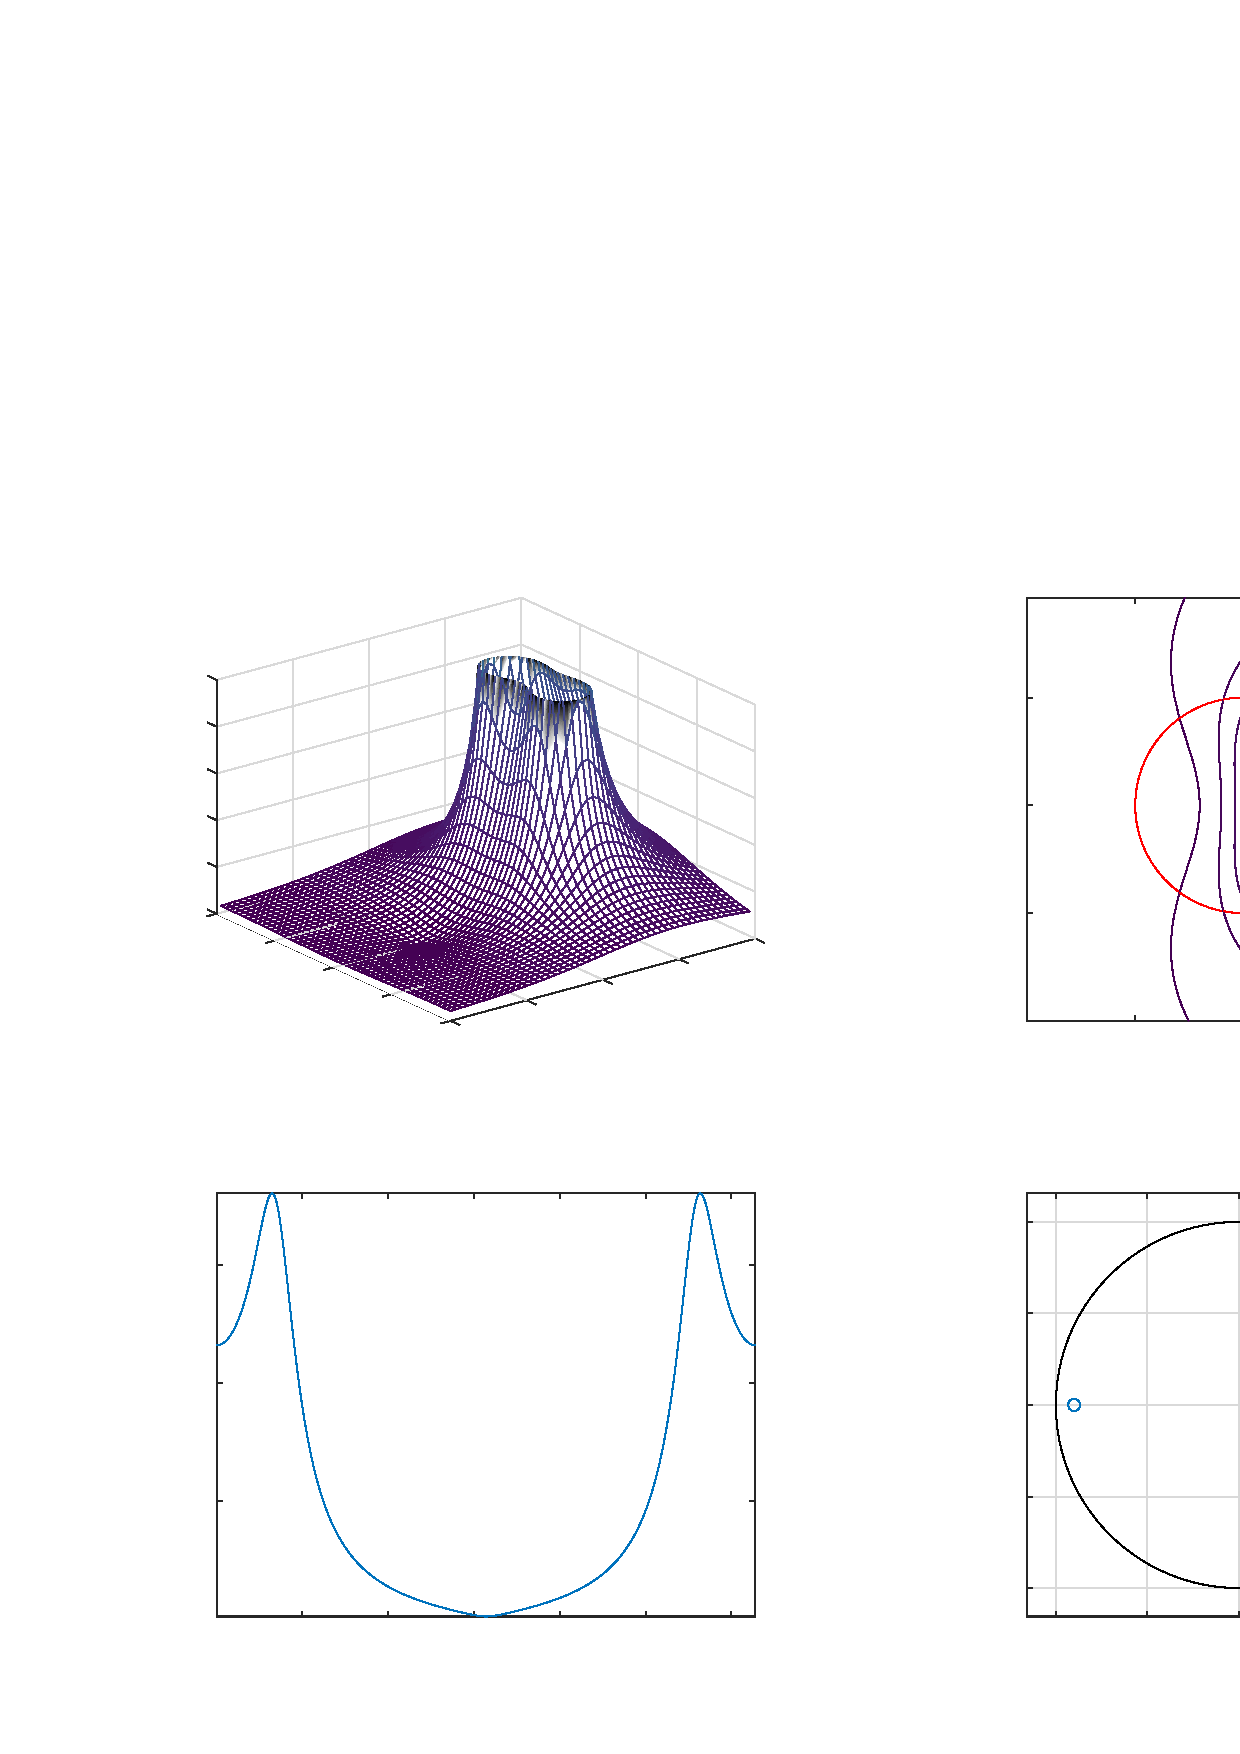
\includegraphics[scale=1]{octaves/zTransformExample3b-inc}
\end{picture}%
\begin{picture}(800,600)(0,0)
\fontsize{13}{0}\selectfont\put(204.784,348.828){\makebox(0,0)[tr]{\textcolor[rgb]{0.15,0.15,0.15}{{-2}}}}
\fontsize{13}{0}\selectfont\put(176.717,361.679){\makebox(0,0)[tr]{\textcolor[rgb]{0.15,0.15,0.15}{{-1}}}}
\fontsize{15}{0}\selectfont\put(131.651,359.53){\makebox(0,0)[tr]{\textcolor[rgb]{0.15,0.15,0.15}{{zi}}}}
\fontsize{13}{0}\selectfont\put(148.651,374.53){\makebox(0,0)[tr]{\textcolor[rgb]{0.15,0.15,0.15}{{0}}}}
\fontsize{13}{0}\selectfont\put(120.584,387.381){\makebox(0,0)[tr]{\textcolor[rgb]{0.15,0.15,0.15}{{1}}}}
\fontsize{13}{0}\selectfont\put(92.517,400.233){\makebox(0,0)[tr]{\textcolor[rgb]{0.15,0.15,0.15}{{2}}}}
\fontsize{13}{0}\selectfont\put(227.087,346.969){\makebox(0,0)[tl]{\textcolor[rgb]{0.15,0.15,0.15}{{-2}}}}
\fontsize{13}{0}\selectfont\put(93.1802,408.283){\makebox(0,0)[br]{\textcolor[rgb]{0.15,0.15,0.15}{{0}}}}
\fontsize{15}{0}\selectfont\put(317.242,351.692){\makebox(0,0)[tl]{\textcolor[rgb]{0.15,0.15,0.15}{{zr}}}}
\fontsize{13}{0}\selectfont\put(336.819,376.553){\makebox(0,0)[tl]{\textcolor[rgb]{0.15,0.15,0.15}{{1}}}}
\fontsize{13}{0}\selectfont\put(373.396,386.414){\makebox(0,0)[tl]{\textcolor[rgb]{0.15,0.15,0.15}{{2}}}}
\fontsize{13}{0}\selectfont\put(263.664,356.831){\makebox(0,0)[tl]{\textcolor[rgb]{0.15,0.15,0.15}{{-1}}}}
\fontsize{13}{0}\selectfont\put(300.242,366.692){\makebox(0,0)[tl]{\textcolor[rgb]{0.15,0.15,0.15}{{0}}}}
\fontsize{13}{0}\selectfont\put(93.1802,430.728){\makebox(0,0)[br]{\textcolor[rgb]{0.15,0.15,0.15}{{1}}}}
\fontsize{13}{0}\selectfont\put(93.1802,453.173){\makebox(0,0)[br]{\textcolor[rgb]{0.15,0.15,0.15}{{2}}}}
\fontsize{15}{0}\selectfont\put(81.1802,464.396){\rotatebox{90}{\makebox(0,0)[b]{\textcolor[rgb]{0.15,0.15,0.15}{{|W|}}}}}
\fontsize{13}{0}\selectfont\put(93.1802,475.619){\makebox(0,0)[br]{\textcolor[rgb]{0.15,0.15,0.15}{{3}}}}
\fontsize{13}{0}\selectfont\put(93.1802,498.064){\makebox(0,0)[br]{\textcolor[rgb]{0.15,0.15,0.15}{{4}}}}
\fontsize{13}{0}\selectfont\put(93.1802,520.51){\makebox(0,0)[br]{\textcolor[rgb]{0.15,0.15,0.15}{{5}}}}
\fontsize{13}{0}\selectfont\put(493.174,341.498){\makebox(0,0)[t]{\textcolor[rgb]{0.15,0.15,0.15}{{-2}}}}
\fontsize{13}{0}\selectfont\put(544.886,341.498){\makebox(0,0)[t]{\textcolor[rgb]{0.15,0.15,0.15}{{-1}}}}
\fontsize{13}{0}\selectfont\put(596.599,341.498){\makebox(0,0)[t]{\textcolor[rgb]{0.15,0.15,0.15}{{0}}}}
\fontsize{13}{0}\selectfont\put(648.312,341.498){\makebox(0,0)[t]{\textcolor[rgb]{0.15,0.15,0.15}{{1}}}}
\fontsize{13}{0}\selectfont\put(486.223,351.924){\makebox(0,0)[r]{\textcolor[rgb]{0.15,0.15,0.15}{{-2}}}}
\fontsize{13}{0}\selectfont\put(486.223,403.636){\makebox(0,0)[r]{\textcolor[rgb]{0.15,0.15,0.15}{{-1}}}}
\fontsize{13}{0}\selectfont\put(486.223,455.349){\makebox(0,0)[r]{\textcolor[rgb]{0.15,0.15,0.15}{{0}}}}
\fontsize{13}{0}\selectfont\put(486.223,507.062){\makebox(0,0)[r]{\textcolor[rgb]{0.15,0.15,0.15}{{1}}}}
\fontsize{15}{0}\selectfont\put(469.223,453.462){\rotatebox{90}{\makebox(0,0)[b]{\textcolor[rgb]{0.15,0.15,0.15}{{zi}}}}}
\fontsize{15}{0}\selectfont\put(594.712,326.498){\makebox(0,0)[t]{\textcolor[rgb]{0.15,0.15,0.15}{{zr}}}}
\fontsize{15}{0}\selectfont\put(594.712,565){\makebox(0,0)[b]{\textcolor[rgb]{0,0,0}{{|W|}}}}
\fontsize{13}{0}\selectfont\put(104,55.5749){\makebox(0,0)[t]{\textcolor[rgb]{0.15,0.15,0.15}{{0}}}}
\fontsize{13}{0}\selectfont\put(145.175,55.5749){\makebox(0,0)[t]{\textcolor[rgb]{0.15,0.15,0.15}{{1}}}}
\fontsize{13}{0}\selectfont\put(186.349,55.5749){\makebox(0,0)[t]{\textcolor[rgb]{0.15,0.15,0.15}{{2}}}}
\fontsize{13}{0}\selectfont\put(227.524,55.5749){\makebox(0,0)[t]{\textcolor[rgb]{0.15,0.15,0.15}{{3}}}}
\fontsize{13}{0}\selectfont\put(268.698,55.5749){\makebox(0,0)[t]{\textcolor[rgb]{0.15,0.15,0.15}{{4}}}}
\fontsize{13}{0}\selectfont\put(309.873,55.5749){\makebox(0,0)[t]{\textcolor[rgb]{0.15,0.15,0.15}{{5}}}}
\fontsize{13}{0}\selectfont\put(351.048,55.5749){\makebox(0,0)[t]{\textcolor[rgb]{0.15,0.15,0.15}{{6}}}}
\fontsize{13}{0}\selectfont\put(97.0639,121.596){\makebox(0,0)[r]{\textcolor[rgb]{0.15,0.15,0.15}{{2}}}}
\fontsize{13}{0}\selectfont\put(97.0639,178.199){\makebox(0,0)[r]{\textcolor[rgb]{0.15,0.15,0.15}{{4}}}}
\fontsize{13}{0}\selectfont\put(97.0639,234.802){\makebox(0,0)[r]{\textcolor[rgb]{0.15,0.15,0.15}{{6}}}}
\fontsize{15}{0}\selectfont\put(85.0639,167.538){\rotatebox{90}{\makebox(0,0)[b]{\textcolor[rgb]{0.15,0.15,0.15}{{|W|   (lin)}}}}}
\fontsize{15}{0}\selectfont\put(233.288,40.5749){\makebox(0,0)[t]{\textcolor[rgb]{0.15,0.15,0.15}{{omega}}}}
\fontsize{13}{0}\selectfont\put(506.8,55.5749){\makebox(0,0)[t]{\textcolor[rgb]{0.15,0.15,0.15}{{-1}}}}
\fontsize{13}{0}\selectfont\put(550.756,55.5749){\makebox(0,0)[t]{\textcolor[rgb]{0.15,0.15,0.15}{{-0.5}}}}
\fontsize{13}{0}\selectfont\put(594.712,55.5749){\makebox(0,0)[t]{\textcolor[rgb]{0.15,0.15,0.15}{{0}}}}
\fontsize{13}{0}\selectfont\put(638.668,55.5749){\makebox(0,0)[t]{\textcolor[rgb]{0.15,0.15,0.15}{{0.5}}}}
\fontsize{13}{0}\selectfont\put(682.624,55.5749){\makebox(0,0)[t]{\textcolor[rgb]{0.15,0.15,0.15}{{1}}}}
\fontsize{13}{0}\selectfont\put(486.223,79.6263){\makebox(0,0)[r]{\textcolor[rgb]{0.15,0.15,0.15}{{-1}}}}
\fontsize{13}{0}\selectfont\put(486.223,123.582){\makebox(0,0)[r]{\textcolor[rgb]{0.15,0.15,0.15}{{-0.5}}}}
\fontsize{13}{0}\selectfont\put(486.223,167.538){\makebox(0,0)[r]{\textcolor[rgb]{0.15,0.15,0.15}{{0}}}}
\fontsize{13}{0}\selectfont\put(486.223,211.494){\makebox(0,0)[r]{\textcolor[rgb]{0.15,0.15,0.15}{{0.5}}}}
\fontsize{13}{0}\selectfont\put(486.223,255.45){\makebox(0,0)[r]{\textcolor[rgb]{0.15,0.15,0.15}{{1}}}}
\end{picture}

}\caption{Plot of $z$-Transform $W_{3b}(z) = \frac{ (z + 0.9) } {(z - 0.6 - j*0.5)(z - 0.6 + j*0.5)}$. This version of plots in Figure~\ref{oct:zTransformExample3} adds an additional zero in location $\xi = -0.9$. The zero influences the overall magnitude, and forces an even stricter valley nearby point $(-1,0)$ of z-plane.}\label{oct:zTransformExample3b}
\end{center}
\end{figure*}

\begin{figure*}[ht]
\begin{center}
\scalebox{0.6}{
    % Title: Figure 1
% Creator: GL2PS 1.4.2, (C) 1999-2020 C. Geuzaine
% For: Octave
% CreationDate: Wed Nov 23 09:16:33 2022
\setlength{\unitlength}{1pt}
\begin{picture}(0,0)
\includegraphics[scale=1]{octaves/zTransformExample4-inc}
\end{picture}%
\begin{picture}(800,600)(0,0)
\fontsize{13}{0}\selectfont\put(204.784,348.828){\makebox(0,0)[tr]{\textcolor[rgb]{0.15,0.15,0.15}{{-2}}}}
\fontsize{13}{0}\selectfont\put(176.717,361.679){\makebox(0,0)[tr]{\textcolor[rgb]{0.15,0.15,0.15}{{-1}}}}
\fontsize{15}{0}\selectfont\put(131.651,359.53){\makebox(0,0)[tr]{\textcolor[rgb]{0.15,0.15,0.15}{{zi}}}}
\fontsize{13}{0}\selectfont\put(148.651,374.53){\makebox(0,0)[tr]{\textcolor[rgb]{0.15,0.15,0.15}{{0}}}}
\fontsize{13}{0}\selectfont\put(120.584,387.381){\makebox(0,0)[tr]{\textcolor[rgb]{0.15,0.15,0.15}{{1}}}}
\fontsize{13}{0}\selectfont\put(92.517,400.233){\makebox(0,0)[tr]{\textcolor[rgb]{0.15,0.15,0.15}{{2}}}}
\fontsize{13}{0}\selectfont\put(227.087,346.969){\makebox(0,0)[tl]{\textcolor[rgb]{0.15,0.15,0.15}{{-2}}}}
\fontsize{13}{0}\selectfont\put(93.1802,408.283){\makebox(0,0)[br]{\textcolor[rgb]{0.15,0.15,0.15}{{0}}}}
\fontsize{15}{0}\selectfont\put(81.1802,464.396){\rotatebox{90}{\makebox(0,0)[b]{\textcolor[rgb]{0.15,0.15,0.15}{{|W|}}}}}
\fontsize{13}{0}\selectfont\put(336.819,376.553){\makebox(0,0)[tl]{\textcolor[rgb]{0.15,0.15,0.15}{{1}}}}
\fontsize{13}{0}\selectfont\put(373.396,386.414){\makebox(0,0)[tl]{\textcolor[rgb]{0.15,0.15,0.15}{{2}}}}
\fontsize{13}{0}\selectfont\put(263.664,356.831){\makebox(0,0)[tl]{\textcolor[rgb]{0.15,0.15,0.15}{{-1}}}}
\fontsize{13}{0}\selectfont\put(300.242,366.692){\makebox(0,0)[tl]{\textcolor[rgb]{0.15,0.15,0.15}{{0}}}}
\fontsize{15}{0}\selectfont\put(317.242,351.692){\makebox(0,0)[tl]{\textcolor[rgb]{0.15,0.15,0.15}{{zr}}}}
\fontsize{13}{0}\selectfont\put(93.1802,430.728){\makebox(0,0)[br]{\textcolor[rgb]{0.15,0.15,0.15}{{1}}}}
\fontsize{13}{0}\selectfont\put(93.1802,453.173){\makebox(0,0)[br]{\textcolor[rgb]{0.15,0.15,0.15}{{2}}}}
\fontsize{13}{0}\selectfont\put(93.1802,475.619){\makebox(0,0)[br]{\textcolor[rgb]{0.15,0.15,0.15}{{3}}}}
\fontsize{13}{0}\selectfont\put(93.1802,498.064){\makebox(0,0)[br]{\textcolor[rgb]{0.15,0.15,0.15}{{4}}}}
\fontsize{13}{0}\selectfont\put(93.1802,520.51){\makebox(0,0)[br]{\textcolor[rgb]{0.15,0.15,0.15}{{5}}}}
\fontsize{13}{0}\selectfont\put(493.174,341.498){\makebox(0,0)[t]{\textcolor[rgb]{0.15,0.15,0.15}{{-2}}}}
\fontsize{13}{0}\selectfont\put(544.886,341.498){\makebox(0,0)[t]{\textcolor[rgb]{0.15,0.15,0.15}{{-1}}}}
\fontsize{13}{0}\selectfont\put(596.599,341.498){\makebox(0,0)[t]{\textcolor[rgb]{0.15,0.15,0.15}{{0}}}}
\fontsize{13}{0}\selectfont\put(648.312,341.498){\makebox(0,0)[t]{\textcolor[rgb]{0.15,0.15,0.15}{{1}}}}
\fontsize{13}{0}\selectfont\put(486.223,351.924){\makebox(0,0)[r]{\textcolor[rgb]{0.15,0.15,0.15}{{-2}}}}
\fontsize{13}{0}\selectfont\put(486.223,403.636){\makebox(0,0)[r]{\textcolor[rgb]{0.15,0.15,0.15}{{-1}}}}
\fontsize{13}{0}\selectfont\put(486.223,455.349){\makebox(0,0)[r]{\textcolor[rgb]{0.15,0.15,0.15}{{0}}}}
\fontsize{13}{0}\selectfont\put(486.223,507.062){\makebox(0,0)[r]{\textcolor[rgb]{0.15,0.15,0.15}{{1}}}}
\fontsize{15}{0}\selectfont\put(469.223,453.462){\rotatebox{90}{\makebox(0,0)[b]{\textcolor[rgb]{0.15,0.15,0.15}{{zi}}}}}
\fontsize{15}{0}\selectfont\put(594.712,326.498){\makebox(0,0)[t]{\textcolor[rgb]{0.15,0.15,0.15}{{zr}}}}
\fontsize{15}{0}\selectfont\put(594.712,565){\makebox(0,0)[b]{\textcolor[rgb]{0,0,0}{{|W|}}}}
\fontsize{13}{0}\selectfont\put(104,55.5748){\makebox(0,0)[t]{\textcolor[rgb]{0.15,0.15,0.15}{{0}}}}
\fontsize{13}{0}\selectfont\put(145.175,55.5748){\makebox(0,0)[t]{\textcolor[rgb]{0.15,0.15,0.15}{{1}}}}
\fontsize{13}{0}\selectfont\put(186.349,55.5748){\makebox(0,0)[t]{\textcolor[rgb]{0.15,0.15,0.15}{{2}}}}
\fontsize{13}{0}\selectfont\put(227.524,55.5748){\makebox(0,0)[t]{\textcolor[rgb]{0.15,0.15,0.15}{{3}}}}
\fontsize{13}{0}\selectfont\put(268.698,55.5748){\makebox(0,0)[t]{\textcolor[rgb]{0.15,0.15,0.15}{{4}}}}
\fontsize{13}{0}\selectfont\put(309.873,55.5748){\makebox(0,0)[t]{\textcolor[rgb]{0.15,0.15,0.15}{{5}}}}
\fontsize{13}{0}\selectfont\put(351.048,55.5748){\makebox(0,0)[t]{\textcolor[rgb]{0.15,0.15,0.15}{{6}}}}
\fontsize{13}{0}\selectfont\put(97.0639,89.5239){\makebox(0,0)[r]{\textcolor[rgb]{0.15,0.15,0.15}{{0.2}}}}
\fontsize{13}{0}\selectfont\put(97.0639,116.235){\makebox(0,0)[r]{\textcolor[rgb]{0.15,0.15,0.15}{{0.4}}}}
\fontsize{13}{0}\selectfont\put(97.0639,142.946){\makebox(0,0)[r]{\textcolor[rgb]{0.15,0.15,0.15}{{0.6}}}}
\fontsize{13}{0}\selectfont\put(97.0639,169.657){\makebox(0,0)[r]{\textcolor[rgb]{0.15,0.15,0.15}{{0.8}}}}
\fontsize{13}{0}\selectfont\put(97.0639,196.368){\makebox(0,0)[r]{\textcolor[rgb]{0.15,0.15,0.15}{{1}}}}
\fontsize{13}{0}\selectfont\put(97.0639,223.08){\makebox(0,0)[r]{\textcolor[rgb]{0.15,0.15,0.15}{{1.2}}}}
\fontsize{13}{0}\selectfont\put(97.0639,249.791){\makebox(0,0)[r]{\textcolor[rgb]{0.15,0.15,0.15}{{1.4}}}}
\fontsize{15}{0}\selectfont\put(74.0639,167.538){\rotatebox{90}{\makebox(0,0)[b]{\textcolor[rgb]{0.15,0.15,0.15}{{|W|   (lin)}}}}}
\fontsize{15}{0}\selectfont\put(233.288,40.5749){\makebox(0,0)[t]{\textcolor[rgb]{0.15,0.15,0.15}{{omega}}}}
\fontsize{13}{0}\selectfont\put(506.8,55.5749){\makebox(0,0)[t]{\textcolor[rgb]{0.15,0.15,0.15}{{-1}}}}
\fontsize{13}{0}\selectfont\put(550.756,55.5749){\makebox(0,0)[t]{\textcolor[rgb]{0.15,0.15,0.15}{{-0.5}}}}
\fontsize{13}{0}\selectfont\put(594.712,55.5749){\makebox(0,0)[t]{\textcolor[rgb]{0.15,0.15,0.15}{{0}}}}
\fontsize{13}{0}\selectfont\put(638.668,55.5749){\makebox(0,0)[t]{\textcolor[rgb]{0.15,0.15,0.15}{{0.5}}}}
\fontsize{13}{0}\selectfont\put(682.624,55.5749){\makebox(0,0)[t]{\textcolor[rgb]{0.15,0.15,0.15}{{1}}}}
\fontsize{13}{0}\selectfont\put(486.223,79.6263){\makebox(0,0)[r]{\textcolor[rgb]{0.15,0.15,0.15}{{-1}}}}
\fontsize{13}{0}\selectfont\put(486.223,123.582){\makebox(0,0)[r]{\textcolor[rgb]{0.15,0.15,0.15}{{-0.5}}}}
\fontsize{13}{0}\selectfont\put(486.223,167.538){\makebox(0,0)[r]{\textcolor[rgb]{0.15,0.15,0.15}{{0}}}}
\fontsize{13}{0}\selectfont\put(486.223,211.494){\makebox(0,0)[r]{\textcolor[rgb]{0.15,0.15,0.15}{{0.5}}}}
\fontsize{13}{0}\selectfont\put(486.223,255.45){\makebox(0,0)[r]{\textcolor[rgb]{0.15,0.15,0.15}{{1}}}}
\end{picture}

}\caption{Plot of $z$-Transform $W_4(z) = \frac{ (z - 0.6 + j*0.8)(z - 0.6 - j*0.8) } {(z - 0.5 - j*0.7)(z - 0.5 + j*0.7)(z - 0.3)}$. This elaborated example illustrates a plot of $2$ zeros---both located in the unit circle---and $3$ poles, two of which compose a complex--conjugate pair. Absolutely, the zeros will force the magnitude to collapse to $0$ at the frequency corresponding to their locations; on contrary, the three poles will influence the magnitude on the other way around. What happens is that, in practice, the zero will prevail (after all, it's located closer to the unit circle we are evaluating the magnitude on), but still its effects are counterbalanced by the presence of two nearby poles.}\label{oct:zTransformExample4}
\end{center}
\end{figure*}

\begin{figure*}[ht]
\begin{center}
\scalebox{0.6}{
    % Title: Figure 1
% Creator: GL2PS 1.4.2, (C) 1999-2020 C. Geuzaine
% For: Octave
% CreationDate: Wed Nov 23 09:35:06 2022
\setlength{\unitlength}{1pt}
\begin{picture}(0,0)
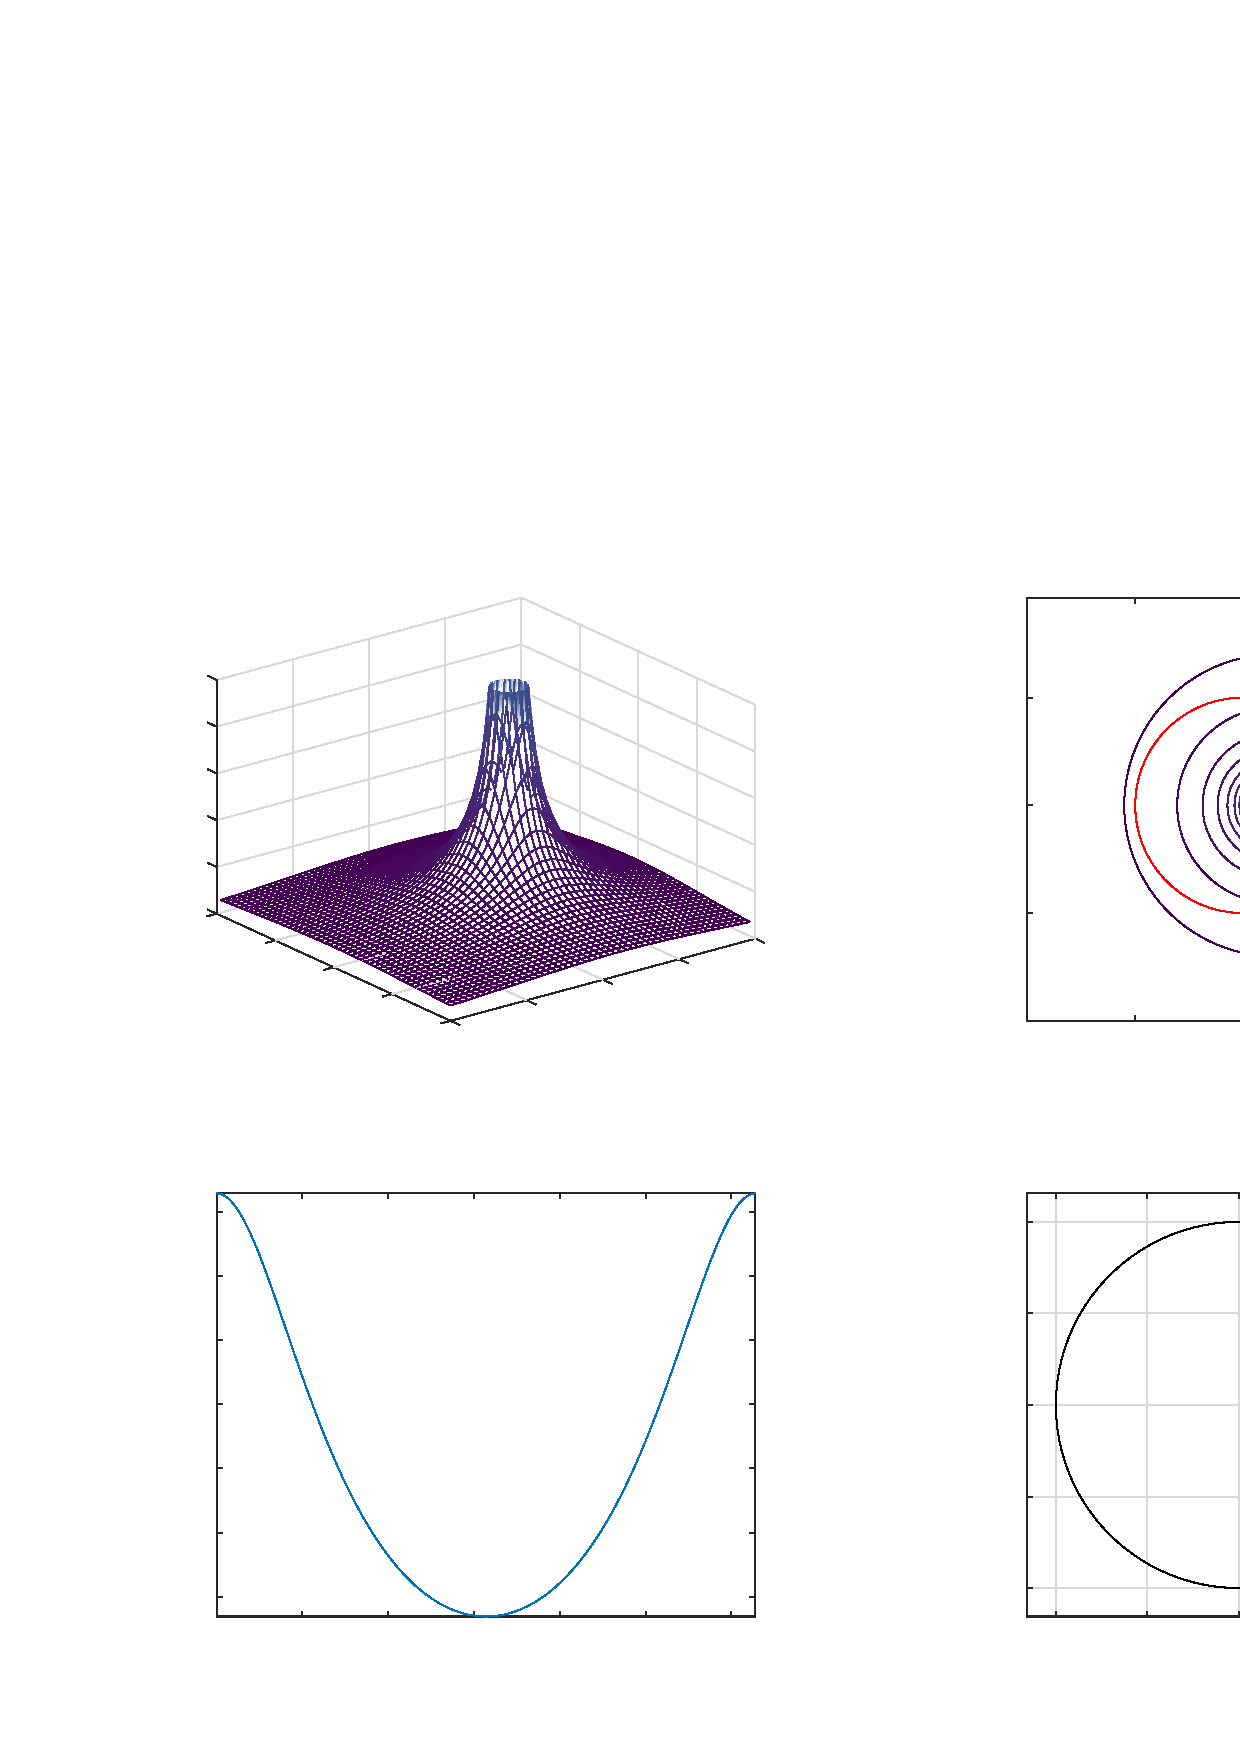
\includegraphics[scale=1]{octaves/zTransformExample4b-inc}
\end{picture}%
\begin{picture}(800,600)(0,0)
\fontsize{15}{0}\selectfont\put(131.651,359.53){\makebox(0,0)[tr]{\textcolor[rgb]{0.15,0.15,0.15}{{zi}}}}
\fontsize{15}{0}\selectfont\put(317.242,351.692){\makebox(0,0)[tl]{\textcolor[rgb]{0.15,0.15,0.15}{{zr}}}}
\fontsize{13}{0}\selectfont\put(373.396,386.414){\makebox(0,0)[tl]{\textcolor[rgb]{0.15,0.15,0.15}{{2}}}}
\fontsize{13}{0}\selectfont\put(92.517,400.233){\makebox(0,0)[tr]{\textcolor[rgb]{0.15,0.15,0.15}{{2}}}}
\fontsize{13}{0}\selectfont\put(93.1802,408.283){\makebox(0,0)[br]{\textcolor[rgb]{0.15,0.15,0.15}{{0}}}}
\fontsize{13}{0}\selectfont\put(336.819,376.553){\makebox(0,0)[tl]{\textcolor[rgb]{0.15,0.15,0.15}{{1}}}}
\fontsize{13}{0}\selectfont\put(300.242,366.692){\makebox(0,0)[tl]{\textcolor[rgb]{0.15,0.15,0.15}{{0}}}}
\fontsize{13}{0}\selectfont\put(204.784,348.828){\makebox(0,0)[tr]{\textcolor[rgb]{0.15,0.15,0.15}{{-2}}}}
\fontsize{13}{0}\selectfont\put(176.717,361.679){\makebox(0,0)[tr]{\textcolor[rgb]{0.15,0.15,0.15}{{-1}}}}
\fontsize{13}{0}\selectfont\put(148.651,374.53){\makebox(0,0)[tr]{\textcolor[rgb]{0.15,0.15,0.15}{{0}}}}
\fontsize{13}{0}\selectfont\put(120.584,387.381){\makebox(0,0)[tr]{\textcolor[rgb]{0.15,0.15,0.15}{{1}}}}
\fontsize{13}{0}\selectfont\put(227.087,346.969){\makebox(0,0)[tl]{\textcolor[rgb]{0.15,0.15,0.15}{{-2}}}}
\fontsize{13}{0}\selectfont\put(263.664,356.831){\makebox(0,0)[tl]{\textcolor[rgb]{0.15,0.15,0.15}{{-1}}}}
\fontsize{13}{0}\selectfont\put(93.1802,430.728){\makebox(0,0)[br]{\textcolor[rgb]{0.15,0.15,0.15}{{1}}}}
\fontsize{13}{0}\selectfont\put(93.1802,453.173){\makebox(0,0)[br]{\textcolor[rgb]{0.15,0.15,0.15}{{2}}}}
\fontsize{15}{0}\selectfont\put(81.1802,464.396){\rotatebox{90}{\makebox(0,0)[b]{\textcolor[rgb]{0.15,0.15,0.15}{{|W|}}}}}
\fontsize{13}{0}\selectfont\put(93.1802,475.619){\makebox(0,0)[br]{\textcolor[rgb]{0.15,0.15,0.15}{{3}}}}
\fontsize{13}{0}\selectfont\put(93.1802,498.064){\makebox(0,0)[br]{\textcolor[rgb]{0.15,0.15,0.15}{{4}}}}
\fontsize{13}{0}\selectfont\put(93.1802,520.51){\makebox(0,0)[br]{\textcolor[rgb]{0.15,0.15,0.15}{{5}}}}
\fontsize{13}{0}\selectfont\put(493.174,341.498){\makebox(0,0)[t]{\textcolor[rgb]{0.15,0.15,0.15}{{-2}}}}
\fontsize{13}{0}\selectfont\put(544.886,341.498){\makebox(0,0)[t]{\textcolor[rgb]{0.15,0.15,0.15}{{-1}}}}
\fontsize{13}{0}\selectfont\put(596.599,341.498){\makebox(0,0)[t]{\textcolor[rgb]{0.15,0.15,0.15}{{0}}}}
\fontsize{13}{0}\selectfont\put(648.312,341.498){\makebox(0,0)[t]{\textcolor[rgb]{0.15,0.15,0.15}{{1}}}}
\fontsize{13}{0}\selectfont\put(486.223,351.924){\makebox(0,0)[r]{\textcolor[rgb]{0.15,0.15,0.15}{{-2}}}}
\fontsize{13}{0}\selectfont\put(486.223,403.636){\makebox(0,0)[r]{\textcolor[rgb]{0.15,0.15,0.15}{{-1}}}}
\fontsize{13}{0}\selectfont\put(486.223,455.349){\makebox(0,0)[r]{\textcolor[rgb]{0.15,0.15,0.15}{{0}}}}
\fontsize{13}{0}\selectfont\put(486.223,507.062){\makebox(0,0)[r]{\textcolor[rgb]{0.15,0.15,0.15}{{1}}}}
\fontsize{15}{0}\selectfont\put(469.223,453.462){\rotatebox{90}{\makebox(0,0)[b]{\textcolor[rgb]{0.15,0.15,0.15}{{zi}}}}}
\fontsize{15}{0}\selectfont\put(594.712,326.498){\makebox(0,0)[t]{\textcolor[rgb]{0.15,0.15,0.15}{{zr}}}}
\fontsize{15}{0}\selectfont\put(594.712,565){\makebox(0,0)[b]{\textcolor[rgb]{0,0,0}{{|W|}}}}
\fontsize{13}{0}\selectfont\put(104,55.5748){\makebox(0,0)[t]{\textcolor[rgb]{0.15,0.15,0.15}{{0}}}}
\fontsize{13}{0}\selectfont\put(145.175,55.5748){\makebox(0,0)[t]{\textcolor[rgb]{0.15,0.15,0.15}{{1}}}}
\fontsize{13}{0}\selectfont\put(186.349,55.5748){\makebox(0,0)[t]{\textcolor[rgb]{0.15,0.15,0.15}{{2}}}}
\fontsize{13}{0}\selectfont\put(227.524,55.5748){\makebox(0,0)[t]{\textcolor[rgb]{0.15,0.15,0.15}{{3}}}}
\fontsize{13}{0}\selectfont\put(268.698,55.5748){\makebox(0,0)[t]{\textcolor[rgb]{0.15,0.15,0.15}{{4}}}}
\fontsize{13}{0}\selectfont\put(309.873,55.5748){\makebox(0,0)[t]{\textcolor[rgb]{0.15,0.15,0.15}{{5}}}}
\fontsize{13}{0}\selectfont\put(351.048,55.5748){\makebox(0,0)[t]{\textcolor[rgb]{0.15,0.15,0.15}{{6}}}}
\fontsize{13}{0}\selectfont\put(97.0639,75.4768){\makebox(0,0)[r]{\textcolor[rgb]{0.15,0.15,0.15}{{0.8}}}}
\fontsize{13}{0}\selectfont\put(97.0639,106.277){\makebox(0,0)[r]{\textcolor[rgb]{0.15,0.15,0.15}{{0.9}}}}
\fontsize{13}{0}\selectfont\put(97.0639,137.077){\makebox(0,0)[r]{\textcolor[rgb]{0.15,0.15,0.15}{{1}}}}
\fontsize{13}{0}\selectfont\put(97.0639,167.877){\makebox(0,0)[r]{\textcolor[rgb]{0.15,0.15,0.15}{{1.1}}}}
\fontsize{13}{0}\selectfont\put(97.0639,198.677){\makebox(0,0)[r]{\textcolor[rgb]{0.15,0.15,0.15}{{1.2}}}}
\fontsize{13}{0}\selectfont\put(97.0639,229.477){\makebox(0,0)[r]{\textcolor[rgb]{0.15,0.15,0.15}{{1.3}}}}
\fontsize{13}{0}\selectfont\put(97.0639,260.276){\makebox(0,0)[r]{\textcolor[rgb]{0.15,0.15,0.15}{{1.4}}}}
\fontsize{15}{0}\selectfont\put(74.0639,167.538){\rotatebox{90}{\makebox(0,0)[b]{\textcolor[rgb]{0.15,0.15,0.15}{{|W|   (lin)}}}}}
\fontsize{15}{0}\selectfont\put(233.288,40.5749){\makebox(0,0)[t]{\textcolor[rgb]{0.15,0.15,0.15}{{omega}}}}
\fontsize{13}{0}\selectfont\put(506.8,55.5749){\makebox(0,0)[t]{\textcolor[rgb]{0.15,0.15,0.15}{{-1}}}}
\fontsize{13}{0}\selectfont\put(550.756,55.5749){\makebox(0,0)[t]{\textcolor[rgb]{0.15,0.15,0.15}{{-0.5}}}}
\fontsize{13}{0}\selectfont\put(594.712,55.5749){\makebox(0,0)[t]{\textcolor[rgb]{0.15,0.15,0.15}{{0}}}}
\fontsize{13}{0}\selectfont\put(638.668,55.5749){\makebox(0,0)[t]{\textcolor[rgb]{0.15,0.15,0.15}{{0.5}}}}
\fontsize{13}{0}\selectfont\put(682.624,55.5749){\makebox(0,0)[t]{\textcolor[rgb]{0.15,0.15,0.15}{{1}}}}
\fontsize{13}{0}\selectfont\put(486.223,79.6263){\makebox(0,0)[r]{\textcolor[rgb]{0.15,0.15,0.15}{{-1}}}}
\fontsize{13}{0}\selectfont\put(486.223,123.582){\makebox(0,0)[r]{\textcolor[rgb]{0.15,0.15,0.15}{{-0.5}}}}
\fontsize{13}{0}\selectfont\put(486.223,167.538){\makebox(0,0)[r]{\textcolor[rgb]{0.15,0.15,0.15}{{0}}}}
\fontsize{13}{0}\selectfont\put(486.223,211.494){\makebox(0,0)[r]{\textcolor[rgb]{0.15,0.15,0.15}{{0.5}}}}
\fontsize{13}{0}\selectfont\put(486.223,255.45){\makebox(0,0)[r]{\textcolor[rgb]{0.15,0.15,0.15}{{1}}}}
\end{picture}

}\caption{Plot of $z$-Transform $W_{4b}(z) = \frac{ (z - 0.6 + j*0.8)(z - 0.6 - j*0.8) } {(z - 0.6 - j*0.8)(z - 0.6 + j*0.8)(z - 0.3)} = \frac { 1 } {(z - 0.3)}$. In fact, following the previous example, moving the two poles to the zeros produces a \emph{zero--pole cancellation}. Due to the cancellation, the effect of both poles and zeros is completely nullified, and the system behaves exactly like there was only a pole at $\lambda = 0.3$ in the first place.}\label{oct:zTransformExample4b}
\end{center}
\end{figure*}

\clearpage

\section{Types of Transfer Functions}

There are two possible classifications when it comes to transfer functions:
\begin{itemize}
    \item based on \emph{magnitude} $|H(e^{j\omega})|$ of frequency response, by looking at the shape of the \emph{magnitude function};
    \item based on \emph{phase} $|\theta(\omega)|$ of frequency response, by considering the \emph{phase function};
\end{itemize}

A rather common approach is considering the \textbf{ideal} magnitude response---an ideal magnitude response is a magnitude response of a digital filter that is equal to $1$ at the frequencies that should pass, and equal to $0$ for all frequencies that should be filtered out. This means that the filter is actually a perfect rectangle, and the filtering will be practically perfect. Of course, this is unachievable in practice.

The range of frequencies that are allowed to pass in an ideal filter are said to be \textbf{passband}, while the range of frequencies that are filtered out for the same ideal filter are called \textbf{stopband}. Although it is possible to design a filter which is either a complete passband or a complete stopband, any decent filter would filter out and let pass at least some frequencies to be really useful.

\begin{center}
    \begin{tikzpicture}
        \node[blue] at (0, -.7) {Lowpass};
        \draw[-stealth] (-1.5, 0) -- (1.5, 0) node[anchor=north west] {$\omega$};
        \draw[-stealth] (0, 0) -- (0, 1.2) node[anchor=south west] {$H_{LP}(e^{j\omega})$};
        \draw[thick] node[anchor=north east] {$-\omega_c$} (-0.4, -0) -- (-0.4, 0.8) -- (0.4, 0.8) -- (0.4, -0) node[anchor=north] {$\omega_c$};
        \node[label=north east:{$1$}] at (0, .7){};
        \node[label=south:{$\pi$}] at (1.2, 0){};
        \node[label=south:{$-\pi$}] at (-1.2, 0){};
        \draw (1.2, -0.03) -- (1.2, +0.03);
        \draw (-1.2, -0.03) -- (-1.2, +0.03);
        \draw (-0.03, 0.8) -- (0.03, 0.8);
    \end{tikzpicture}
    \begin{tikzpicture}
        \node[blue] at (0, -.7) {Highpass};
        \draw[-stealth] (-1.5, 0) -- (1.5, 0) node[anchor=north west] {$\omega$};
        \draw[-stealth] (0, 0) -- (0, 1.2) node[anchor=south west] {$H_{HP}(e^{j\omega})$};
        \draw[thick] (-1.2, 0.8) -| (-0.4, -0) node[anchor=north] {$-\omega_c$} ;
        \draw[thick] (0.4, -0) node[anchor=north] {$\omega_c$} |- (1.2, 0.8);
        \draw (-0.03, 0.8) -- (0.03, 0.8);
        \node[label=north east:{$1$}] at (0, .7){};
        \node[label=south:{$\pi$}] at (1.2, 0){};
        \node[label=south:{$-\pi$}] at (-1.2, 0){};
        \draw (1.2, -0.03) -- (1.2, +0.03);
        \draw (-1.2, -0.03) -- (-1.2, +0.03);
    \end{tikzpicture}

    \begin{tikzpicture}
        \node[blue] at (0, -.7) {Bandpass};
        \draw[-stealth] (-1.5, 0) -- (1.5, 0) node[anchor=north west] {$\omega$};
        \draw[-stealth] (0, 0) -- (0, 1.2) node[anchor=south west] {$H_{BP}(e^{j\omega})$};
        \draw[thick] (-0.8, -0) -- (-0.8, 0.8) -- (-0.4, 0.8) -- (-0.4, -0);
        \draw[thick] (+0.8, -0) -- (+0.8, 0.8) -- (+0.4, 0.8) -- (+0.4, -0);
        \node[label=north east:{$1$}] at (0, .7){};
        \node[label=south:{$\pi$}] at (1.2, 0){};
        \node[label=south:{$-\pi$}] at (-1.2, 0){};
        \draw (1.2, -0.03) -- (1.2, +0.03);
        \draw (-1.2, -0.03) -- (-1.2, +0.03);
        \draw (-0.03, 0.8) -- (0.03, 0.8);
    \end{tikzpicture}
    \begin{tikzpicture}
        \node[blue] at (0, -.7) {Bandstop};
        \draw[-stealth] (-1.5, 0) -- (1.5, 0) node[anchor=north west] {$\omega$};
        \draw[-stealth] (0, 0) -- (0, 1.2) node[anchor=south west] {$H_{BS}(e^{j\omega})$};
        \draw[thick] (-1.2, 0.8) -| (-0.8, 0);
        \draw[thick] (+1.2, 0.8) -| (+0.8, 0);
        \draw[thick] (-0.4, -0) -- (-0.4, 0.8) -- (0.4, 0.8) -- (0.4, -0);
        \node[label=north east:{$1$}] at (0, .7){};
        \node[label=south:{$\pi$}] at (1.2, 0){};
        \node[label=south:{$-\pi$}] at (-1.2, 0){};
        \draw (1.2, -0.03) -- (1.2, +0.03);
        \draw (-1.2, -0.03) -- (-1.2, +0.03);
        \draw (-0.03, 0.8) -- (0.03, 0.8);
    \end{tikzpicture}
\end{center}

Therefore, there are $4$ kinds of ideal filters, that act like in the following descriptions:
\begin{description}
    \item[Lowpass ideal filter] A lowpass ideal filter is a \emph{passband} in frequencies $0 \leq \omega \leq \omega_c$ and a \emph{stopband} in range $\omega_c \leq \omega \leq \pi$.
    \item[Highpass ideal filter] A highpass ideal filter is a \emph{passband} in frequencies $\omega_c \leq \omega \leq \pi$ and a \emph{stopband} in range $0 \leq \omega \leq \omega_c$.
    \item[Bandpass ideal filter] A bandpass ideal filter is a \emph{passband} in frequencies $\omega_{c1} \leq \omega \leq \omega_{c2}$ and a \emph{stopband} in frequencies $0 \leq \omega \leq \omega_{c1}$ and $\omega_{c2} \leq \omega \leq \pi$.
    \item[Bandstop ideal filter] A bandstop ideal filter is a \emph{passband} in frequencies $0 \leq \omega \leq \omega_{c1}$ and $\omega_{c2} \leq \omega \leq \pi$ and a \emph{stopband} in range $\omega_{c1} \leq \omega \leq \omega_{c2}$.
\end{description}
Frequencies for which the filter goes from $1$ to $0$ and vice versa are said to be \textbf{cutoff frequencies}.


As we have previously seen in Equation~\ref{eqn:inverseDiscreteTimeFourierTransformRectangle}, the inverse DTFT for an ideal lowpass filter---that is, a rectangle---is a \emph{sinc} function
\[
    h_{LP} = \frac {\sin {\omega_c n}}{\pi n} = \sinc {\omega_c n}, -\infty < n < \infty;
\]
moreover, it has been shown that the above impulse response is not absolutely summable. Hence, the corresponding transfer function is not BIBO stable, as the Theorem~\ref{thm:ltiBiboStability} dictates. The sequence $h_{LP}[n]$ is neither causal nor finite (they are doubly-infinite), and for this reason the ideal filters are not feasible in practice. Even the remaining $3$ types of filters also possess doubly infinite length, noncausal impusle responses and are ultimately not absolutely summable. The conclusion is that no ideal filter with immediate cutoff (rectangle frequency response) can be possibly realized, not withouth employing an infinite dimensional LTI filter---which of course is not feasible in practice.

\begin{center}
    \begin{tikzpicture}
        \draw[-stealth] (0,0) -- (7.5, 0) node[anchor=west] {$\omega$};
        \draw[-stealth] (0,0) -- (0, 4.5) node[anchor=south] {$\left|G(e^{j\omega})\right|$};
        \draw[ultra thick] plot[samples=200,domain=0:7] function {4 / (1 + sqrt((0.70*x)**10))};

        \draw (0.05, 4) -- (-0.05, 4) node[anchor=east] {$1 + \delta_p$};
        \draw[dashed] (0, 4) -- (1, 4);
        \draw (0.05, 3.5) -- (-0.05, 3.5) node[anchor=east] {$1 - \delta_p$};
        \draw[dashed] (0, 3.5) -- (1, 3.5);
        \draw (0.05, 0.5) -- (-0.05, 0.5) node[anchor=east] {$\delta_s$};
        \draw[dashed] (0, 0.5) -- (7, 0.5);
        \draw (1, 0.05) -- (1, -0.05) node[anchor=north] {$\omega_p$};
        \draw[dashed] (1, 0) -- (1, 4);
        \draw (2.1, 0.05) -- (2.1, -0.05) node[anchor=north] {$\omega_s$};
        \draw[dashed] (2.1, 0) -- (2.1, 4);
        \draw (7, 0.05) -- (7, -0.05) node[anchor=north] {$\pi$};
        \node[rotate=90] at (0.5, 2) {Passband};
        \node[rotate=90] at (1.55, 3.5) {Transition band};
        \node at (4, 1) {Stopband};
    \end{tikzpicture}
\end{center}

The above figure shows a generic lowpass filter design, with its constraints. A lowpass filter must respect the \emph{passbands constraints} to be in margin between $1 \pm \delta_p$, and the \emph{stopband constraints} to stay in the margin from $0$ to $\delta_s$. Deciding about and imposing those constraints are indeed what it takes to start designing a lowpass filter, as the constraints $\delta_p$, $\delta_s$, $\omega_p$ and $\omega_s$ will force the filter to respect a specific behavior.

Passband constraints force the filter magnitude to stay in a specific range of values---namely, $1 \pm \delta_p$---so that the filter an effectively \emph{allow to pass} frequencies up to frequency $\omega_p$. Stopband constraints force---instead---the filter to \emph{block} all frequencies from $\omega_s$ to $\pi$. In stopband, the filter shall not exceed values of $\delta_s$. Since no real filter is an ideal filter, a \textbf{transition band} must be endorsed in order for the filter to transition from the passband to the stopband. A specific range of frequencies---from $\omega_p$ to $\omega_s$---cannot be properly handled by the filter, as its magnitude in such range will exhibit an undefined behavior.

\section{Bounded Real Transfer Functions}

\textbf{Bounded Real Transfer Functions} are a class of functions that is bounded to the unity for all of its frequency range. That is,
\begin{defin}[Bounded Real Transfer Function]
    A causal stable real-coefficient transfer function $H(z)$ is said to be a \emph{bounded real (BR) transfer function} if
    \begin{equation}\label{eqn:boundedRealTransferFunctionCondition}
        \left|H(e^{j\omega})\right| \leq 1
    \end{equation}
    for all values of $\omega$.
\end{defin}

Let now $x[n]$ and $y[n]$ be the input and the output of a digital filter that is characterized by a BR transfer function $H(z)$ such as above. Let also $X(e^{j\omega})$ and $Y(e^{j\omega})$ denote their DTFTs. The condition as in~\ref{eqn:boundedRealTransferFunctionCondition} implies that 
\[
    \left|Y(e^{j\omega})\right|^2 \leq \left|X(e^{j\omega})\right|^2.
\]
By integrating from $-\pi$ to $\pi$ and applying Parseval's Theorem, one soon obtains that
\begin{equation}\label{eqn:boundedRealTransferFunctionPassiveStructure}
    \sum_{n=-\infty}^\infty\left|y[n]\right|^2 \leq \sum_{n=-\infty}^\infty\left|x[n]\right|^2.
\end{equation}

Equation~\ref{eqn:boundedRealTransferFunctionPassiveStructure} entails that for all finite-energy inputs, the energy of the output is \emph{less than or at most equal} to the input energy. Any digital filter characterized by a BR transfer function can be viewed as a \textbf{passive structure}. Only in the specific case in which
\[
    \left|H(e^{j\omega})\right| = 1
\]
one has that the output energy is equal to the input energy---such a digital filter is a \textbf{lossless system}. The latter is so important that is deserves its own special definition.

\begin{defin}[Lossless Bounded Real Transfer Function]
    A causal stable real-coefficient transfer function $H(z)$ is said to be a \emph{lossless bounded real (LBR) transfer function} if
    \begin{equation}\label{eqn:losslessBoundedRealTransferFunctionCondition}
        \left|H(e^{j\omega})\right| = 1
    \end{equation}
    for all values of $\omega$.
\end{defin}

Both BR and LBR transfer functions are the keys to the realization of digital filters with \emph{low coefficient sensitivity}.

\subsubsection{Example}
As an example, consider a causal IIR transfer function
\[
    H(z) = \frac{
        K
    } {
        1 - \alpha z^{-1}
    },
    0 < |\alpha| < 1
\]
where $K$ and $\alpha$ are real constants. Its square-magnitude function is given by the following
\[
    \left|H(e^{j\omega})\right|^2 = H(z)H(z^{-1})\Bigr\rvert_{z=e^{j\omega}} =
        \frac {
            K^2
        } { 
            (1 + \alpha^2) - 2\alpha\cos{\omega}
        }.
\]


\begin{figure*}[ht]
\begin{center}
\scalebox{0.6}{
    % Title: Figure 1
% Creator: GL2PS 1.4.2, (C) 1999-2020 C. Geuzaine
% For: Octave
% CreationDate: Wed Nov 23 15:54:34 2022
\setlength{\unitlength}{1pt}
\begin{picture}(0,0)
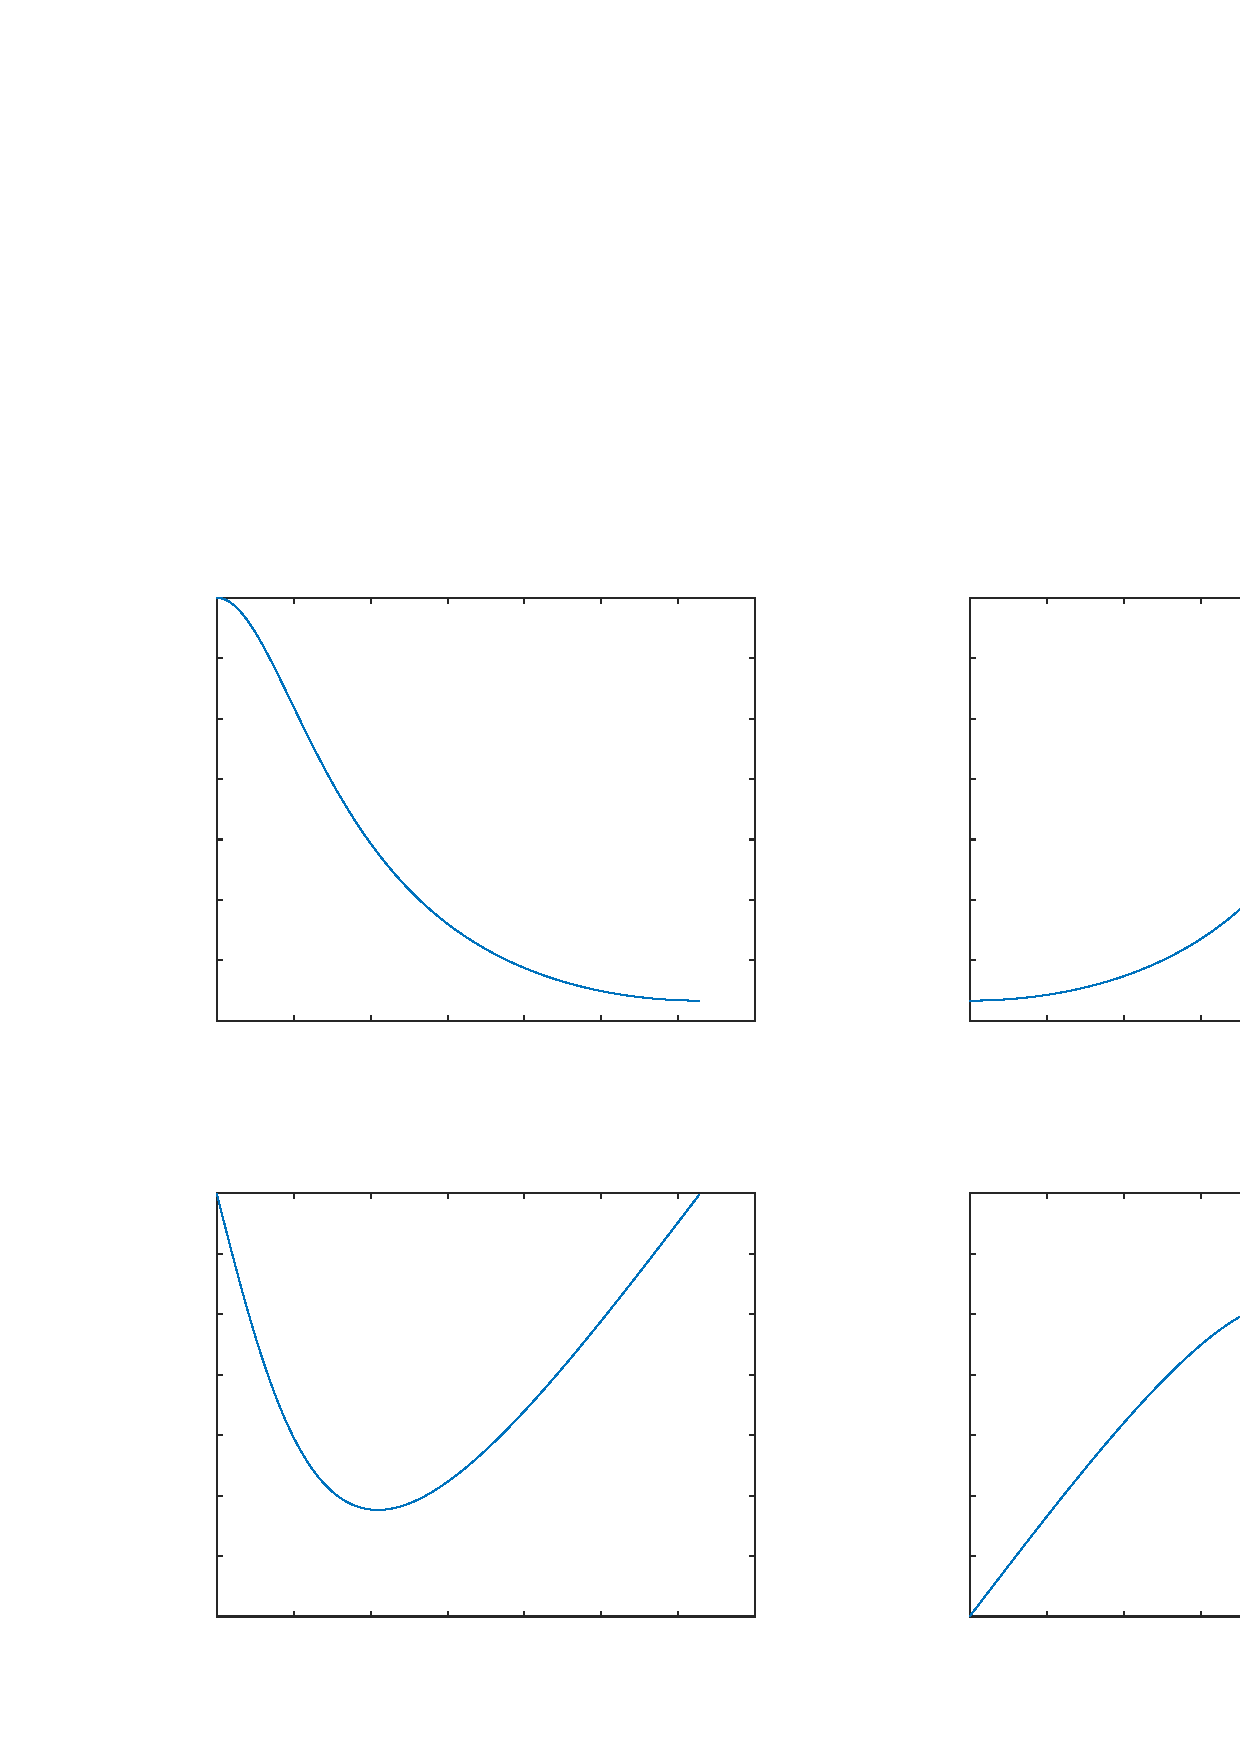
\includegraphics[scale=1]{octaves/boundedRealTransferFunctionsExample-inc}
\end{picture}%
\begin{picture}(800,600)(0,0)
\fontsize{13}{0}\selectfont\put(104,341.538){\makebox(0,0)[t]{\textcolor[rgb]{0.15,0.15,0.15}{{0}}}}
\fontsize{13}{0}\selectfont\put(140.937,341.538){\makebox(0,0)[t]{\textcolor[rgb]{0.15,0.15,0.15}{{0.5}}}}
\fontsize{13}{0}\selectfont\put(177.873,341.538){\makebox(0,0)[t]{\textcolor[rgb]{0.15,0.15,0.15}{{1}}}}
\fontsize{13}{0}\selectfont\put(214.81,341.538){\makebox(0,0)[t]{\textcolor[rgb]{0.15,0.15,0.15}{{1.5}}}}
\fontsize{13}{0}\selectfont\put(251.747,341.538){\makebox(0,0)[t]{\textcolor[rgb]{0.15,0.15,0.15}{{2}}}}
\fontsize{13}{0}\selectfont\put(288.683,341.538){\makebox(0,0)[t]{\textcolor[rgb]{0.15,0.15,0.15}{{2.5}}}}
\fontsize{13}{0}\selectfont\put(325.62,341.538){\makebox(0,0)[t]{\textcolor[rgb]{0.15,0.15,0.15}{{3}}}}
\fontsize{13}{0}\selectfont\put(362.556,341.538){\makebox(0,0)[t]{\textcolor[rgb]{0.15,0.15,0.15}{{3.5}}}}
\fontsize{13}{0}\selectfont\put(97.0766,351.944){\makebox(0,0)[r]{\textcolor[rgb]{0.15,0.15,0.15}{{0.3}}}}
\fontsize{13}{0}\selectfont\put(97.0766,380.952){\makebox(0,0)[r]{\textcolor[rgb]{0.15,0.15,0.15}{{0.4}}}}
\fontsize{13}{0}\selectfont\put(97.0766,409.96){\makebox(0,0)[r]{\textcolor[rgb]{0.15,0.15,0.15}{{0.5}}}}
\fontsize{13}{0}\selectfont\put(97.0766,438.968){\makebox(0,0)[r]{\textcolor[rgb]{0.15,0.15,0.15}{{0.6}}}}
\fontsize{13}{0}\selectfont\put(97.0766,467.976){\makebox(0,0)[r]{\textcolor[rgb]{0.15,0.15,0.15}{{0.7}}}}
\fontsize{13}{0}\selectfont\put(97.0766,496.984){\makebox(0,0)[r]{\textcolor[rgb]{0.15,0.15,0.15}{{0.8}}}}
\fontsize{13}{0}\selectfont\put(97.0766,525.992){\makebox(0,0)[r]{\textcolor[rgb]{0.15,0.15,0.15}{{0.9}}}}
\fontsize{13}{0}\selectfont\put(97.0766,555){\makebox(0,0)[r]{\textcolor[rgb]{0.15,0.15,0.15}{{1}}}}
\fontsize{15}{0}\selectfont\put(233.278,565){\makebox(0,0)[b]{\textcolor[rgb]{0,0,0}{{K = 0.5, alpha = 0.5}}}}
\fontsize{13}{0}\selectfont\put(104,55.5941){\makebox(0,0)[t]{\textcolor[rgb]{0.15,0.15,0.15}{{0}}}}
\fontsize{13}{0}\selectfont\put(140.937,55.5941){\makebox(0,0)[t]{\textcolor[rgb]{0.15,0.15,0.15}{{0.5}}}}
\fontsize{13}{0}\selectfont\put(177.873,55.5941){\makebox(0,0)[t]{\textcolor[rgb]{0.15,0.15,0.15}{{1}}}}
\fontsize{13}{0}\selectfont\put(214.81,55.5941){\makebox(0,0)[t]{\textcolor[rgb]{0.15,0.15,0.15}{{1.5}}}}
\fontsize{13}{0}\selectfont\put(251.747,55.5941){\makebox(0,0)[t]{\textcolor[rgb]{0.15,0.15,0.15}{{2}}}}
\fontsize{13}{0}\selectfont\put(288.683,55.5941){\makebox(0,0)[t]{\textcolor[rgb]{0.15,0.15,0.15}{{2.5}}}}
\fontsize{13}{0}\selectfont\put(325.62,55.5941){\makebox(0,0)[t]{\textcolor[rgb]{0.15,0.15,0.15}{{3}}}}
\fontsize{13}{0}\selectfont\put(362.556,55.5941){\makebox(0,0)[t]{\textcolor[rgb]{0.15,0.15,0.15}{{3.5}}}}
\fontsize{13}{0}\selectfont\put(97.0766,66){\makebox(0,0)[r]{\textcolor[rgb]{0.15,0.15,0.15}{{-0.7}}}}
\fontsize{13}{0}\selectfont\put(97.0766,95.008){\makebox(0,0)[r]{\textcolor[rgb]{0.15,0.15,0.15}{{-0.6}}}}
\fontsize{13}{0}\selectfont\put(97.0766,124.016){\makebox(0,0)[r]{\textcolor[rgb]{0.15,0.15,0.15}{{-0.5}}}}
\fontsize{13}{0}\selectfont\put(97.0766,153.024){\makebox(0,0)[r]{\textcolor[rgb]{0.15,0.15,0.15}{{-0.4}}}}
\fontsize{13}{0}\selectfont\put(97.0766,182.032){\makebox(0,0)[r]{\textcolor[rgb]{0.15,0.15,0.15}{{-0.3}}}}
\fontsize{13}{0}\selectfont\put(97.0766,211.04){\makebox(0,0)[r]{\textcolor[rgb]{0.15,0.15,0.15}{{-0.2}}}}
\fontsize{13}{0}\selectfont\put(97.0766,240.048){\makebox(0,0)[r]{\textcolor[rgb]{0.15,0.15,0.15}{{-0.1}}}}
\fontsize{13}{0}\selectfont\put(97.0766,269.056){\makebox(0,0)[r]{\textcolor[rgb]{0.15,0.15,0.15}{{0}}}}
\fontsize{13}{0}\selectfont\put(465.444,341.538){\makebox(0,0)[t]{\textcolor[rgb]{0.15,0.15,0.15}{{0}}}}
\fontsize{13}{0}\selectfont\put(502.38,341.538){\makebox(0,0)[t]{\textcolor[rgb]{0.15,0.15,0.15}{{0.5}}}}
\fontsize{13}{0}\selectfont\put(539.317,341.538){\makebox(0,0)[t]{\textcolor[rgb]{0.15,0.15,0.15}{{1}}}}
\fontsize{13}{0}\selectfont\put(576.253,341.538){\makebox(0,0)[t]{\textcolor[rgb]{0.15,0.15,0.15}{{1.5}}}}
\fontsize{13}{0}\selectfont\put(613.19,341.538){\makebox(0,0)[t]{\textcolor[rgb]{0.15,0.15,0.15}{{2}}}}
\fontsize{13}{0}\selectfont\put(650.127,341.538){\makebox(0,0)[t]{\textcolor[rgb]{0.15,0.15,0.15}{{2.5}}}}
\fontsize{13}{0}\selectfont\put(687.063,341.538){\makebox(0,0)[t]{\textcolor[rgb]{0.15,0.15,0.15}{{3}}}}
\fontsize{13}{0}\selectfont\put(724,341.538){\makebox(0,0)[t]{\textcolor[rgb]{0.15,0.15,0.15}{{3.5}}}}
\fontsize{13}{0}\selectfont\put(458.52,351.944){\makebox(0,0)[r]{\textcolor[rgb]{0.15,0.15,0.15}{{0.3}}}}
\fontsize{13}{0}\selectfont\put(458.52,380.952){\makebox(0,0)[r]{\textcolor[rgb]{0.15,0.15,0.15}{{0.4}}}}
\fontsize{13}{0}\selectfont\put(458.52,409.96){\makebox(0,0)[r]{\textcolor[rgb]{0.15,0.15,0.15}{{0.5}}}}
\fontsize{13}{0}\selectfont\put(458.52,438.968){\makebox(0,0)[r]{\textcolor[rgb]{0.15,0.15,0.15}{{0.6}}}}
\fontsize{13}{0}\selectfont\put(458.52,467.976){\makebox(0,0)[r]{\textcolor[rgb]{0.15,0.15,0.15}{{0.7}}}}
\fontsize{13}{0}\selectfont\put(458.52,496.984){\makebox(0,0)[r]{\textcolor[rgb]{0.15,0.15,0.15}{{0.8}}}}
\fontsize{13}{0}\selectfont\put(458.52,525.992){\makebox(0,0)[r]{\textcolor[rgb]{0.15,0.15,0.15}{{0.9}}}}
\fontsize{13}{0}\selectfont\put(458.52,555){\makebox(0,0)[r]{\textcolor[rgb]{0.15,0.15,0.15}{{1}}}}
\fontsize{15}{0}\selectfont\put(594.722,565){\makebox(0,0)[b]{\textcolor[rgb]{0,0,0}{{K = 0.5, alpha = -0.5}}}}
\fontsize{13}{0}\selectfont\put(465.444,55.5941){\makebox(0,0)[t]{\textcolor[rgb]{0.15,0.15,0.15}{{0}}}}
\fontsize{13}{0}\selectfont\put(502.38,55.5941){\makebox(0,0)[t]{\textcolor[rgb]{0.15,0.15,0.15}{{0.5}}}}
\fontsize{13}{0}\selectfont\put(539.317,55.5941){\makebox(0,0)[t]{\textcolor[rgb]{0.15,0.15,0.15}{{1}}}}
\fontsize{13}{0}\selectfont\put(576.253,55.5941){\makebox(0,0)[t]{\textcolor[rgb]{0.15,0.15,0.15}{{1.5}}}}
\fontsize{13}{0}\selectfont\put(613.19,55.5941){\makebox(0,0)[t]{\textcolor[rgb]{0.15,0.15,0.15}{{2}}}}
\fontsize{13}{0}\selectfont\put(650.127,55.5941){\makebox(0,0)[t]{\textcolor[rgb]{0.15,0.15,0.15}{{2.5}}}}
\fontsize{13}{0}\selectfont\put(687.063,55.5941){\makebox(0,0)[t]{\textcolor[rgb]{0.15,0.15,0.15}{{3}}}}
\fontsize{13}{0}\selectfont\put(724,55.5941){\makebox(0,0)[t]{\textcolor[rgb]{0.15,0.15,0.15}{{3.5}}}}
\fontsize{13}{0}\selectfont\put(458.52,66){\makebox(0,0)[r]{\textcolor[rgb]{0.15,0.15,0.15}{{0}}}}
\fontsize{13}{0}\selectfont\put(458.52,95.0081){\makebox(0,0)[r]{\textcolor[rgb]{0.15,0.15,0.15}{{0.1}}}}
\fontsize{13}{0}\selectfont\put(458.52,124.016){\makebox(0,0)[r]{\textcolor[rgb]{0.15,0.15,0.15}{{0.2}}}}
\fontsize{13}{0}\selectfont\put(458.52,153.024){\makebox(0,0)[r]{\textcolor[rgb]{0.15,0.15,0.15}{{0.3}}}}
\fontsize{13}{0}\selectfont\put(458.52,182.032){\makebox(0,0)[r]{\textcolor[rgb]{0.15,0.15,0.15}{{0.4}}}}
\fontsize{13}{0}\selectfont\put(458.52,211.04){\makebox(0,0)[r]{\textcolor[rgb]{0.15,0.15,0.15}{{0.5}}}}
\fontsize{13}{0}\selectfont\put(458.52,240.048){\makebox(0,0)[r]{\textcolor[rgb]{0.15,0.15,0.15}{{0.6}}}}
\fontsize{13}{0}\selectfont\put(458.52,269.056){\makebox(0,0)[r]{\textcolor[rgb]{0.15,0.15,0.15}{{0.7}}}}
\end{picture}

}\caption{Plot of magnitude functions and phase functions of $H(z) = \frac{K}{(1 - \alpha z^{-1})}$, for values of $K=0.5$ and $\alpha=\pm 0.5$. The first of the two filters acts as a lowpass filter, while the other one behaves like a highpass filter.}\label{oct:boundedRealTransferFunctionsExample}
\end{center}
\end{figure*}

The function depends on $\omega$ only in the argument of the cosine at the denominator. Hence, maximum value of $\left|H(e^{j\omega})\right|$ is obtained when $2\alpha \cos{\omega}$ in the denominator is a maximum and the minimum value is obtained when the latter is a minimum. For a positive $\alpha > 0$, maximum value of $2\alpha\cos{\omega}$ is precisely equal to $2\alpha$ at $\omega=0$, while its minimum value is the negative $-2\alpha$ at $\omega=\pi$.
Thus, for $\alpha > 0$ the maximum value of the square-magnitude of the transfer function is equal to
\[
    \max{\left|H(e^{j\omega})\right|^2} = \frac {
        K^2
    } {
        (1 - \alpha)^2
    }
\]
at $\omega=0$, and the minimum value is 
\[
    \min{\left|H(e^{j\omega})\right|^2} = \frac {
        K^2
    } {
        (1 + \alpha)^2
    }
\]
at $\omega=\pi$.

It is clear now that the properties of the transfer function all depend on the particular choice of $\alpha$ and $K$. For instance, in order to obtained a maximum value equal to $1$ one can choose $K = \pm(1 - \alpha)$, and in that case the minimum value will become
\[
    \min{\left|H(e^{j\omega})\right|^2} = \frac {
        (1 - \alpha)^2
    } {
        (1 + \alpha)^2
    }.
\]

Therefore, transfer function
\[
    H(z) = \frac{
        K
    } {
        1 - \alpha z^{-1}
    },
    0 < |\alpha| < 1
\]
becomes a \emph{BR transfer function} with the choice $K = \pm(1 - \alpha)$. Figure~\ref{oct:boundedRealTransferFunctionsExample} plots the transfer function magnitude and phase functions.

The output sequence $y[n]$ will be a weighted average $K > 0$ or a `weighted difference' $K < 0$ of $x[n]$ and $y[n-1]$.

\section{Allpass transfer functions}\label{sec:allpassTransferFunctions}
Some transfer functions are completely flat---such systems are said to be \emph{allpass filters} and related transfer functions are \emph{allpass transfer functions}.

\begin{defin}[Allpass Transfer Functions]
    An IIR transfer function $\mathcal A(z)$ with unity magnitude response for all frequencies
    \begin{equation}\label{eqn:allpassTransferFunction}
        \left|\mathcal A(e^{j\omega})\right| = 1
    \end{equation}
    for all $\omega$
    is called an \emph{allpass transfer function}. An $M$-th order causal real-coefficient allpass transfer function has the form
    \begin{equation}\label{eqn:allpassTransferFunctionM}
        \mathcal A_M(z) = \pm\frac {
            d_M + d_{M-1}z^{-1} + \cdots + d_1z^{-M+1} + z^{-M}
        } {
            1 + d_1z^{-1} + \cdots + d_{M-1}z^{-M+1} + d_Mz^{-M}
        }.
    \end{equation}
\end{defin}

\begin{figure*}[ht]
\begin{center}
\scalebox{0.45}{
    % Title: Figure 1
% Creator: GL2PS 1.4.2, (C) 1999-2020 C. Geuzaine
% For: Octave
% CreationDate: Wed Nov 23 16:40:08 2022
\setlength{\unitlength}{1pt}
\begin{picture}(0,0)
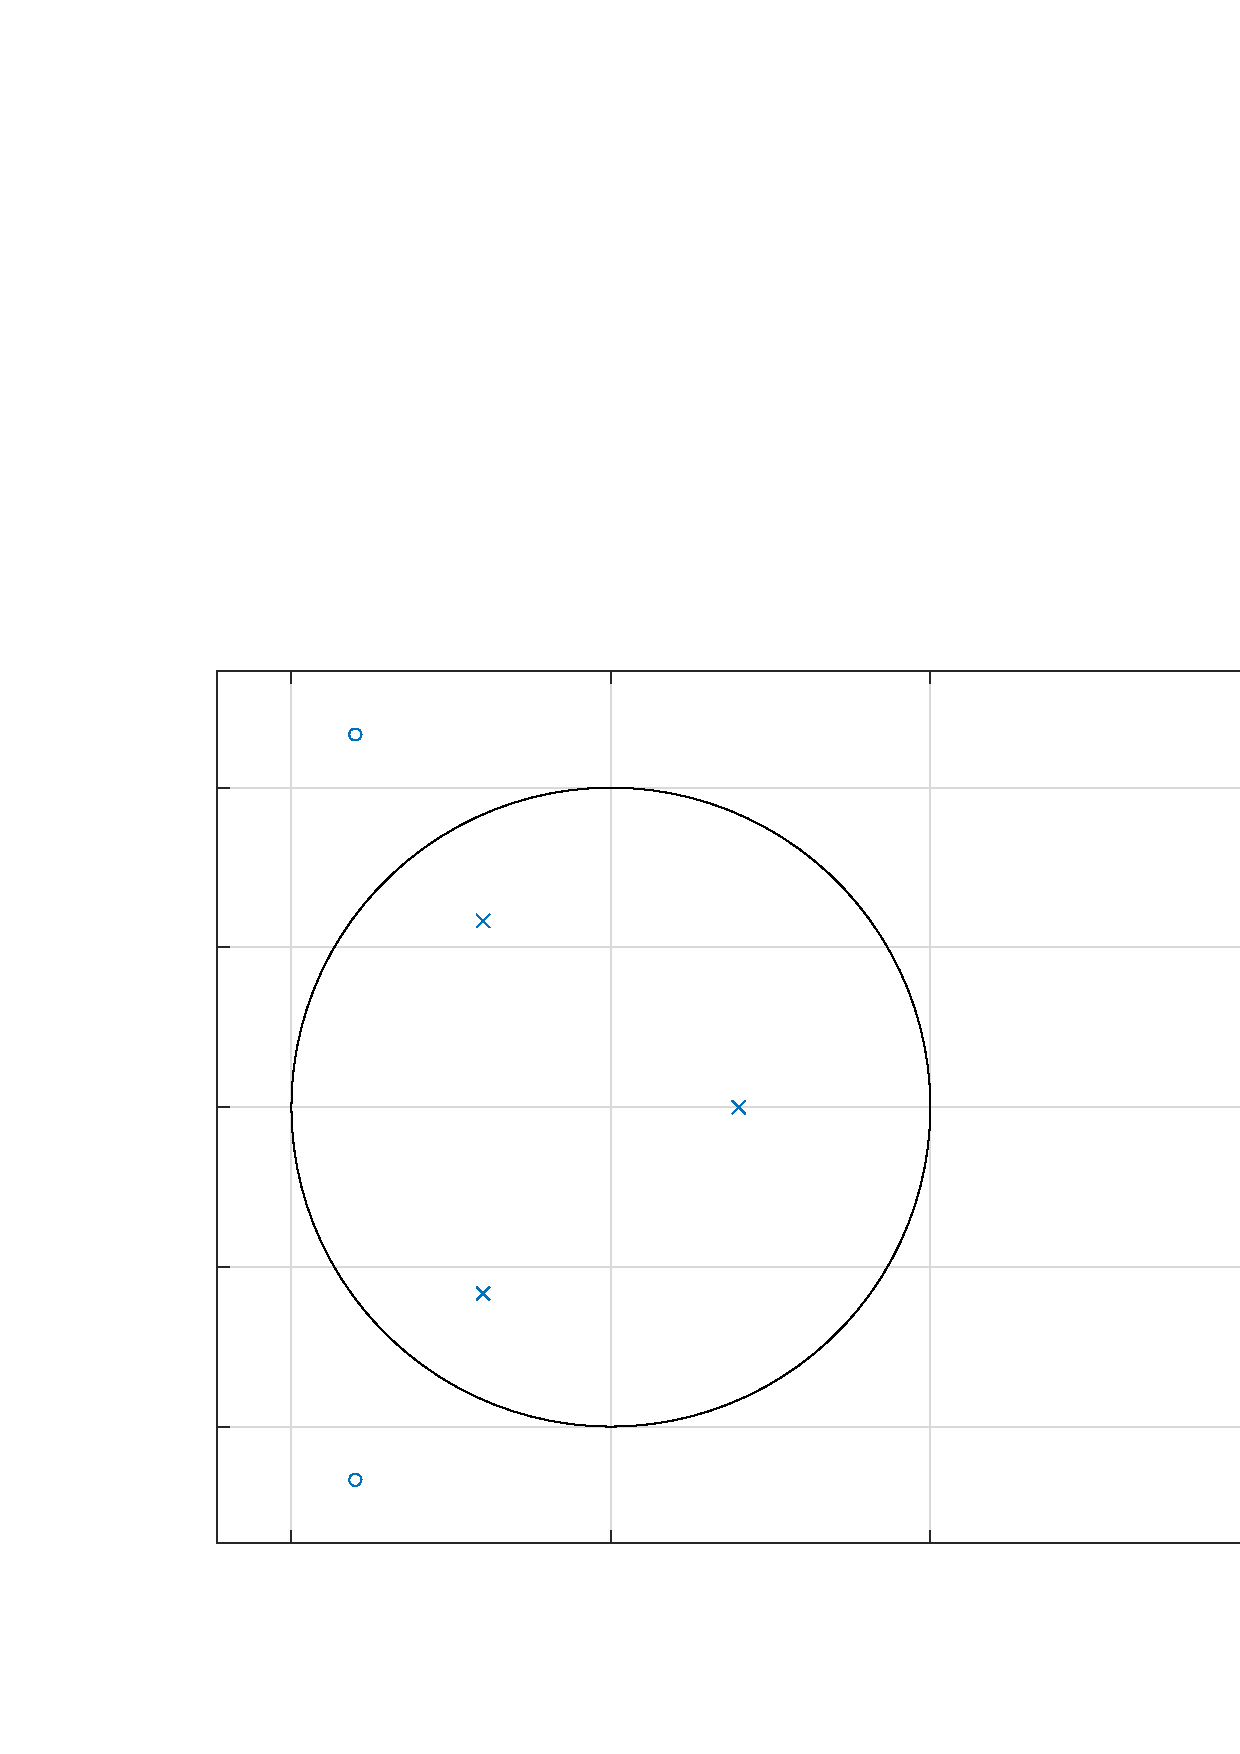
\includegraphics[scale=1]{octaves/allpassTransferFunctionMirrorExample-inc}
\end{picture}%
\begin{picture}(800,600)(0,0)
\fontsize{13}{0}\selectfont\put(139.85,90.6773){\makebox(0,0)[t]{\textcolor[rgb]{0.15,0.15,0.15}{{-1}}}}
\fontsize{13}{0}\selectfont\put(293.221,90.6773){\makebox(0,0)[t]{\textcolor[rgb]{0.15,0.15,0.15}{{0}}}}
\fontsize{13}{0}\selectfont\put(446.591,90.6773){\makebox(0,0)[t]{\textcolor[rgb]{0.15,0.15,0.15}{{1}}}}
\fontsize{13}{0}\selectfont\put(599.962,90.6773){\makebox(0,0)[t]{\textcolor[rgb]{0.15,0.15,0.15}{{2}}}}
\fontsize{13}{0}\selectfont\put(97.0647,157.13){\makebox(0,0)[r]{\textcolor[rgb]{0.15,0.15,0.15}{{-1}}}}
\fontsize{13}{0}\selectfont\put(97.0647,233.815){\makebox(0,0)[r]{\textcolor[rgb]{0.15,0.15,0.15}{{-0.5}}}}
\fontsize{13}{0}\selectfont\put(97.0647,310.5){\makebox(0,0)[r]{\textcolor[rgb]{0.15,0.15,0.15}{{0}}}}
\fontsize{13}{0}\selectfont\put(97.0647,387.185){\makebox(0,0)[r]{\textcolor[rgb]{0.15,0.15,0.15}{{0.5}}}}
\fontsize{13}{0}\selectfont\put(97.0647,463.87){\makebox(0,0)[r]{\textcolor[rgb]{0.15,0.15,0.15}{{1}}}}
\end{picture}

}\caption{Plot of magnitude functions and phase functions of $H(z) = \frac{K}{(1 - \alpha z^{-1})}$, for values of $K=0.5$ and $\alpha=\pm 0.5$. The first of the two filters acts as a lowpass filter, while the other one behaves like a highpass filter.}\label{oct:allpassTransferFunctionMirrorExample}
\end{center}
\end{figure*}

An allpass filter, basically, is a filter which simply \emph{passess all frequences}; Equation~\ref{eqn:allpassTransferFunctionM} gives the form of such filter. By calling the denominator of $\mathcal A_M(z)$ as $D_M(z)$
\[
    D_M(z) = 1 + d_1z^{-1} + \cdots + d_{M-1}z^{-M+1} + d_Mz^{-M},
\]
it follows that one can rewrite $\mathcal A_M(z)$ in the following manner,
\begin{equation}\label{eqn:allpassTransferFunctionMCompact}
    \mathcal A_M(z) = \pm \frac {
        z^{-M} D_M(z^{-1})
    } {
        D_M(z)
    }
\end{equation}
Notice how the above equation will have a zero at $z=\frac 1 r e^{j\varphi}$ for any pole at $z = re^{j\varphi}$, thanks to Equation~\ref{eqn:allpassTransferFunctionMCompact}. In fact, to any pole $z_p = \varkappa$ will correspond a zero at position $z_s = \frac 1 \varkappa$, the reciprocal of the pole. This is the rule of a very important scenario---for this reason, the numerator of a real-coefficient allpass transfer function is said to be the \textbf{mirror-image polynomial} (MIP) of the denominator, and vice versa. Mirror-image polynomials will carry an amount of zeros which is equal to the amount of poles expressed by the denominator, in a position which is determined by the ``reflection'' of the poles in the unit circle---it is from this reflection process that the mirror-image polynomials got their name. One can then employ a convenient notation to denote the mirror-image polynomial of a degree-$M$ polynomial $D_M(z)$, for instance by denoting the polynomial with a tilde,
\begin{equation}\label{eqn:mirrorImagePolynomial}
    \tilde{D}_M(z) = z^{-M}D_M(z^{-1}).
\end{equation}

Later on a similar concept will also prove useful---similarly to the mirror-image polynomial, one can define an \textbf{antimirror-image polynomial} (AIP) as any polynomial that satisfies the following equation,
\begin{equation}\label{eqn:antimirrorImagePolynomial}
    \tilde{D}_M(z) = -z^{-M}D_M(z^{-1}).
\end{equation}


From the mirror-image property, a fundamental property can be inferred: all poles and zeros of a real-coefficient allpass transfer function must exhibit a \emph{mirror-image symmetry} in the z-plane, with respect to the unit circle. For instance, let's plot the following
\[
    \mathcal A_3(z) = \frac {
        -0.2 + 0.18z^{-1} + 0.4z^{-2} + z^{-3}
    } {
        1 + 0.4 z^{-1} + 0.18z^{-2} - 0.2z^{-3}
    }
\]
into Figure~\ref{oct:allpassTransferFunctionMirrorExample}.

To show off that the filter is an allpass filter, that is $\left| \mathcal A_M(e^{j\omega}) \right| = 1$, one has to simply observe that
\[
    \mathcal A_M(z^{-1}) = \pm \frac {
        z^{M} D_M(z)
    } {
        D_M(z^{-1})
    }.
\]

Hence, performing the squared module operation
\[
    \mathcal A_M(z) \mathcal A_M(z^{-1}) = \frac {
        z^{-M} D_M(z^{-1})
    } {
        D_M(z)
    } \cdot \frac {
        z^{M} D_M(z)
    } {
        D_M(z^{-1})
    }
\]
which immediately leads to
\[
    \left|\mathcal A_M(e^{j\omega})\right|^2 = \mathcal A_M(z) \mathcal A_M(z^{-1})\Bigr\rvert_{z=e^{j\omega}} = 1,
\]
a situation which undoubtedly yields
\[
    \left|\mathcal A_M(e^{j\omega})\right| = 1.
\]

In order for a transfer function to be causal, it must lie \emph{inside} the unit circle in the z-plane---else, the region of convergence would not contain the unit circle, and as a result the corresponding transfer function would never be stable. Since all poles should stay inside the unit circle, and since the \emph{mirror-image polynomial} will contain all zeros whose location is given by the mirroring property, all zeros of a causal stable allpass transfer function \emph{must} lie outside the unit circle. Indeed, this is what occurs, as shown in Figure~\ref{oct:allpassTransferFunctionMirrorExample} for an example allpass filter given by the formula
\[
    A_3(z) = \frac{
        -0.2 + 0.18z^{-1} + 0.4z^{-2} + z^{-3}
    } {
        1 + 0.4z^{-1} + 0.18z^{-2} - 0.2z^{-3}
    }, 
\]
and what generally happens for every allpass filter.

\begin{figure*}[ht]
\begin{center}
\scalebox{0.45}{
    % Title: Figure 1
% Creator: GL2PS 1.4.2, (C) 1999-2020 C. Geuzaine
% For: Octave
% CreationDate: Wed Nov 23 16:53:18 2022
\setlength{\unitlength}{1pt}
\begin{picture}(0,0)
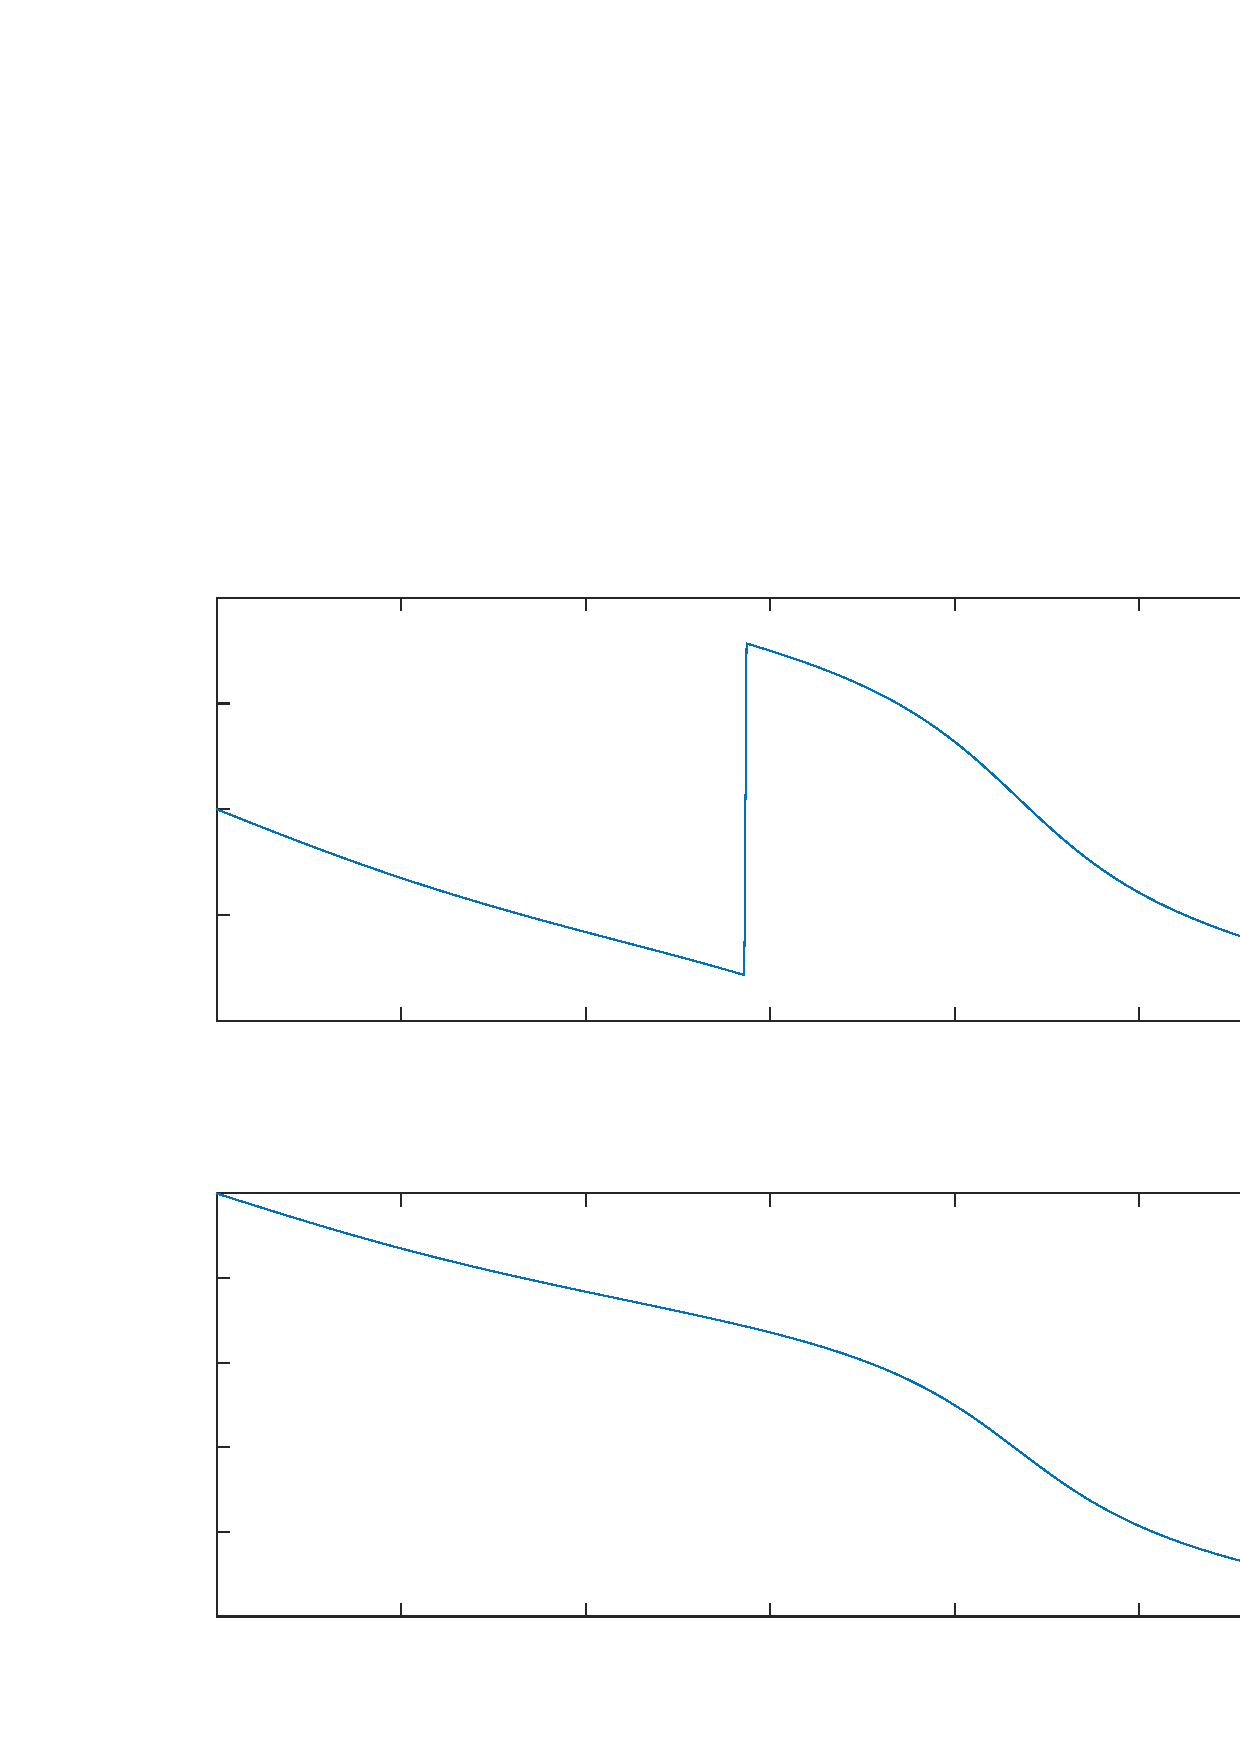
\includegraphics[scale=1]{octaves/allpassTransferFunctionMirrorExamplePhase-inc}
\end{picture}%
\begin{picture}(800,600)(0,0)
\fontsize{13}{0}\selectfont\put(104,341.538){\makebox(0,0)[t]{\textcolor[rgb]{0.15,0.15,0.15}{{0}}}}
\fontsize{13}{0}\selectfont\put(192.571,341.538){\makebox(0,0)[t]{\textcolor[rgb]{0.15,0.15,0.15}{{0.5}}}}
\fontsize{13}{0}\selectfont\put(281.143,341.538){\makebox(0,0)[t]{\textcolor[rgb]{0.15,0.15,0.15}{{1}}}}
\fontsize{13}{0}\selectfont\put(369.714,341.538){\makebox(0,0)[t]{\textcolor[rgb]{0.15,0.15,0.15}{{1.5}}}}
\fontsize{13}{0}\selectfont\put(458.286,341.538){\makebox(0,0)[t]{\textcolor[rgb]{0.15,0.15,0.15}{{2}}}}
\fontsize{13}{0}\selectfont\put(546.857,341.538){\makebox(0,0)[t]{\textcolor[rgb]{0.15,0.15,0.15}{{2.5}}}}
\fontsize{13}{0}\selectfont\put(635.429,341.538){\makebox(0,0)[t]{\textcolor[rgb]{0.15,0.15,0.15}{{3}}}}
\fontsize{13}{0}\selectfont\put(724,341.538){\makebox(0,0)[t]{\textcolor[rgb]{0.15,0.15,0.15}{{3.5}}}}
\fontsize{13}{0}\selectfont\put(97.0647,351.944){\makebox(0,0)[r]{\textcolor[rgb]{0.15,0.15,0.15}{{-4}}}}
\fontsize{13}{0}\selectfont\put(97.0647,402.708){\makebox(0,0)[r]{\textcolor[rgb]{0.15,0.15,0.15}{{-2}}}}
\fontsize{13}{0}\selectfont\put(97.0647,453.472){\makebox(0,0)[r]{\textcolor[rgb]{0.15,0.15,0.15}{{0}}}}
\fontsize{13}{0}\selectfont\put(97.0647,504.236){\makebox(0,0)[r]{\textcolor[rgb]{0.15,0.15,0.15}{{2}}}}
\fontsize{13}{0}\selectfont\put(97.0647,555){\makebox(0,0)[r]{\textcolor[rgb]{0.15,0.15,0.15}{{4}}}}
\fontsize{13}{0}\selectfont\put(104,55.5941){\makebox(0,0)[t]{\textcolor[rgb]{0.15,0.15,0.15}{{0}}}}
\fontsize{13}{0}\selectfont\put(192.571,55.5941){\makebox(0,0)[t]{\textcolor[rgb]{0.15,0.15,0.15}{{0.5}}}}
\fontsize{13}{0}\selectfont\put(281.143,55.5941){\makebox(0,0)[t]{\textcolor[rgb]{0.15,0.15,0.15}{{1}}}}
\fontsize{13}{0}\selectfont\put(369.714,55.5941){\makebox(0,0)[t]{\textcolor[rgb]{0.15,0.15,0.15}{{1.5}}}}
\fontsize{13}{0}\selectfont\put(458.286,55.5941){\makebox(0,0)[t]{\textcolor[rgb]{0.15,0.15,0.15}{{2}}}}
\fontsize{13}{0}\selectfont\put(546.857,55.5941){\makebox(0,0)[t]{\textcolor[rgb]{0.15,0.15,0.15}{{2.5}}}}
\fontsize{13}{0}\selectfont\put(635.429,55.5941){\makebox(0,0)[t]{\textcolor[rgb]{0.15,0.15,0.15}{{3}}}}
\fontsize{13}{0}\selectfont\put(724,55.5941){\makebox(0,0)[t]{\textcolor[rgb]{0.15,0.15,0.15}{{3.5}}}}
\fontsize{13}{0}\selectfont\put(97.0647,66){\makebox(0,0)[r]{\textcolor[rgb]{0.15,0.15,0.15}{{-10}}}}
\fontsize{13}{0}\selectfont\put(97.0647,106.611){\makebox(0,0)[r]{\textcolor[rgb]{0.15,0.15,0.15}{{-8}}}}
\fontsize{13}{0}\selectfont\put(97.0647,147.223){\makebox(0,0)[r]{\textcolor[rgb]{0.15,0.15,0.15}{{-6}}}}
\fontsize{13}{0}\selectfont\put(97.0647,187.834){\makebox(0,0)[r]{\textcolor[rgb]{0.15,0.15,0.15}{{-4}}}}
\fontsize{13}{0}\selectfont\put(97.0647,228.445){\makebox(0,0)[r]{\textcolor[rgb]{0.15,0.15,0.15}{{-2}}}}
\fontsize{13}{0}\selectfont\put(97.0647,269.056){\makebox(0,0)[r]{\textcolor[rgb]{0.15,0.15,0.15}{{0}}}}
\end{picture}

}\caption{Principal value---wrapped and unwrapped---of $3$-rd order allpass function $A_3(z)$. Notice the discointinuity by the amount of $2\pi$ in the phase $\theta(\omega)$; the discontinuity is generally solved by unwrapping the phase as seen in previous chapters.}\label{oct:allpassTransferFunctionMirrorExamplePhase}
\end{center}
\end{figure*}

Let's also plot the phase function of the above filter. Figure~\ref{oct:allpassTransferFunctionMirrorExamplePhase} shows the principal value and the unwrapped phase function of filter $A_3(z)$.
Generally speaking, the unwrapped phase function of \emph{any allpass function} which is also causal and stable is a continuous function in $\omega$.

Some other paramount properties will be highlighted in the next section.

\subsection{Properties of allpass transfer functions}
The main properties of allpass transfer functions that distinguish them from a generic transfer functions are the following three.
\begin{enumerate}
    \item A causal, stable, real-coefficient allpass transfer function is a \emph{lossless bounded real} (LBR) function; or, equivalently, a causal stable allpass filter is a \emph{lossless structure};
    \item the magnitude function of a stable allpass function $A(z)$ satisfies the following
        \[
            |A(z)| = 
            \left\{
                \begin{array}{ll}
                    < 1, & |z| > 1\\
                    = 1, & |z| = 1\\
                    > 1, & |z| < 1
                \end{array}
            \right..
        \]
        Hence, the magnitude in the z-plane is equal to $1$ only in the unit circle, and greater or smaller than $1$ depending---respectively---whether $z$ is inside or outside the unit circle;
    \item let $\tau(\omega)$ be the group delay function of an allpass filter $A(z)$, then
        \[
            \tau(\omega) = -\frac{d}{d\omega}[\theta_c(\omega)]
        \]
        is equal to the negative derivative of the \emph{unwrapped} phase function $\theta_c(\omega)$.
\end{enumerate}
The unwrapped phase function $\theta_c(\omega)$ of $A(z)$, a stable allpass transfer function, is a monotonically decreasing function in $\omega$ so that $\tau(\omega)$ is \emph{everywhere positive} in the range of frequencies $0 < \omega < \pi$. In addition, the group delay of an $M$-th order stable real coefficient allpass transfer function satisfies the following integral equation,
\begin{equation}\label{eqn:allpassIntegralPhaseEquation}
    \int_0^\pi \tau(\omega)d\omega = M\pi.
\end{equation}

Phase rotation for $\omega$ from $0$ to $\pi$ in allpass transfer function will be proportional to the order of the filter. In particular, a single pole will induce a rotation of $\pi$, whilst pole pairs will induce rotations of $2\pi$. Zeros will not introduce any rotation---either single ones or a pair of them will generate $0$ radians rotation. Generally speaking, an allpass transfer function with an order of $M$ will induce a phase rotation of $M\pi$, as indeed expressed by Equation~\ref{eqn:allpassIntegralPhaseEquation}.

\begin{figure*}
\begin{center}
    \begin{tikzpicture}
        \draw[-stealth] (-2.5,0) -- (2.5,0) node[anchor=north west] {$\Re z$};
        \draw[-stealth] (0,-2.5) -- (0,2.5) node[anchor=south east] {$\Im z$};
        \draw (1pt, 1.5) -- (-1pt, 1.5) node[anchor=south west] {$1$};
        \node[draw, circle, dashed, minimum size=3cm] at (0,0) {};
        \node[draw, polez, thick](pole) at (-.7, 0) {};
        \coordinate (O) at (1.5, 0);
        \coordinate (pi) at (-1.5, 0);
        \draw[-latex, thick] (pole) -- (O);
        \draw[-latex, thick] (pole) -- (pi);
        \pic [draw, -stealth, red, "$\pi$", angle radius=4mm, angle eccentricity=1.3] {angle = O--pole--pi};
    \end{tikzpicture}
    \begin{tikzpicture}
        \draw[-stealth] (-2.5,0) -- (2.5,0) node[anchor=north west] {$\Re z$};
        \draw[-stealth] (0,-2.5) -- (0,2.5) node[anchor=south east] {$\Im z$};
        \draw (1pt, 1.5) -- (-1pt, 1.5) node[anchor=south west] {$1$};
        \node[draw, circle, dashed, minimum size=3cm] at (0,0) {};
        \node[draw, polez, thick](ppole) at (.8, 1) {};
        \node[draw, polez, thick](npole) at (.8, -1) {};
        \coordinate (O) at (1.5, 0);
        \coordinate (pi) at (-1.5, 0);
        \coordinate (positiveO) at (1.5, 1);
        \coordinate (positivepi) at (-1.5, 1);
        \coordinate (negativeO) at (1.5, -1);
        \coordinate (negativepi) at (-1.5, -1);
        \draw[dashed] (positiveO) -- (positivepi);
        \draw[dashed] (negativeO) -- (negativepi);
        \draw[-latex] (ppole) -- (O);
        \draw[-latex] (ppole) -- (pi);
        \draw[-latex] (npole) -- (O);
        \draw[-latex] (npole) -- (pi);
        \pic [draw, "$\alpha$",angle radius=5mm, angle eccentricity=.55] {angle = O--ppole--positiveO};
        \pic [draw, "$\pi$", angle radius=4mm, angle eccentricity=1.3] {angle = positiveO--ppole--positivepi};
        \pic [draw, "$\beta$", angle radius=5mm, angle eccentricity=1.2] {angle = positivepi--ppole--pi};
        \pic [draw, "$\alpha$",angle radius=5mm, angle eccentricity=.55] {angle = negativeO--npole--O};
        \pic [draw, "$\beta$", angle radius=5mm, angle eccentricity=1.2] {angle = pi--npole--negativepi};
        \pic [draw, -stealth, red, "$\pi + \alpha + \beta$", angle radius=7mm, angle eccentricity=1.2] {angle = O--ppole--pi};
        \pic [draw, -stealth, blue, "$\pi - \alpha - \beta$", angle radius=6mm, angle eccentricity=1.4] {angle = O--npole--pi};
    \end{tikzpicture}\\
    \begin{tikzpicture}
        \draw[-stealth] (-2.5,0) -- (2.5,0) node[anchor=north west] {$\Re z$};
        \draw[-stealth] (0,-2.5) -- (0,2.5) node[anchor=south east] {$\Im z$};
        \draw (1pt, 1.5) -- (-1pt, 1.5) node[anchor=south west] {$1$};
        \node[draw, circle, dashed, minimum size=3cm] at (0,0) {};
        \node[draw, zeroz, thick](zero) at (-2, 0) {};
        \coordinate (O) at (1.5, 0);
        \coordinate (pi) at (-1.5, 0);
        \draw[-latex, thick] (zero) -- (O);
        \draw[-latex, thick] (zero) -- (pi);
    \end{tikzpicture}
    \begin{tikzpicture}
        \draw[-stealth] (-2.5,0) -- (2.5,0) node[anchor=north west] {$\Re z$};
        \draw[-stealth] (0,-2.5) -- (0,2.5) node[anchor=south east] {$\Im z$};
        \draw (1pt, 1.5) -- (-1pt, 1.5) node[anchor=south west] {$1$};
        \node[draw, circle, dashed, minimum size=3cm] at (0,0) {};
        \node[draw, zeroz, thick](pzero) at (1, 1.6) {};
        \node[draw, zeroz, thick](nzero) at (1, -1.6) {};
        \coordinate (O) at (1.5, 0);
        \coordinate (pi) at (-1.5, 0);
        \coordinate (positiveO) at (1.5, 1);
        \coordinate (positivepi) at (-1.5, 1);
        \coordinate (negativeO) at (1.5, -1);
        \coordinate (negativepi) at (-1.5, -1);
        \draw[-latex] (pzero) -- (O);
        \draw[-latex] (pzero) -- (pi);
        \draw[-latex] (nzero) -- (O);
        \draw[-latex] (nzero) -- (pi);
        \pic [draw, stealth-, red, "$\gamma$", angle radius=5mm, angle eccentricity=.55] {angle = pi--pzero--O};
        \pic [draw, stealth-, blue, "$-\gamma$", angle radius=5mm, angle eccentricity=.55] {angle = O--nzero--pi};
    \end{tikzpicture}
\end{center}\caption{Phase rotation induced by poles and zeros, in example configurations. In red and blue, induced phase rotations by the poles--zeros. On top-left, single pole configuration; top-right, double pole configuration; bottom-left, single zero configuration (notice how the total phase rotation angle is $0$, since the zero can only be located outside the unit circle) and bottom-right, double zero configuration. In the last configuration, the two zeros induce an opposite phase rotation, resulting in no induced rotation. In all poles configurations, the angle of rotation is equal to $M\pi$, with $M$ number of poles.}\label{tikz:phaseRotationPolesZeros}
\end{figure*}

\subsection{Delay equalizers}\label{sec:delayEqualizers}

Allpass filters are not only an abstract concept; they can find their applications in many fields and techniques, for instance as happens for \textbf{delay equalizers}.

Let $G(z)$ be the transfer function of a digital filter designed to meet a prescribed magnitude response. Broadly speaking, what usually happens is that such a filter will introduce a \emph{nonlinear phase response} due to its peculiar shape and properties. Such a phase distortion should be corrected, just like a pair of glasses should be prescribed to a visually impaired person. To correct the phase response it could be useful to employ an allpass filter with a proper phase response---such a filter will leave the magnitude response unscathered (because $|A(e^{j\omega})| = 1$) while modifying the phase response so that the overall cascade of filters will have a \emph{constant group delay} in the band of interest.

\begin{center}
    \begin{tikzpicture}
        \node[draw, thick, rectangle, minimum width=2cm, minimum height=.9cm](G) at (0, 0) {$G(z)$};
        \node[draw, thick, rectangle, minimum width=2cm, minimum height=.9cm](A) at (3, 0) {$A(z)$};
        \draw[-stealth] (-2, 0) -- (G);
        \draw[-stealth] (G) -- (A);
        \draw[-stealth] (A) -- (5, 0);
    \end{tikzpicture}
\end{center}

The overall magnitude will be identical to the magnitude of the original filter $|G(e^{j\omega})A(e^{j\omega})| = |G(e^{j\omega})|$, but the overall group delay will be the \emph{sum} of the group delays of $G(z)$ and $A(z)$.

\section{Classification of transfer functions based on phase characteristics}

Transfer functions can be classified with respect to their unique \emph{phase characteristics}. Commonly, manipulating signals and sequences with filters or digital filters can introduce phase distortions, just like those addressed by the delay equalizers in Section~\ref{sec:delayEqualizers}. Phase distortions can be ignored or not depending on the situation and the application---in some cases, it is absolutely mandatory to correct any distortion of the input signal components' phase, especially in the band of interest. In such situations it is imperative to design a so-called \textbf{zero phase characteristic filter}.

Zero phase characteristic filters are special filters that ideally have a \emph{real} and \emph{non-negative} characteristic. Unfortunately, it is not possible to build \emph{causal} digital filters with zero phase---therefore it is only possible to operate such zero phase characteristic filters on application that do not require \emph{real-time processing}. To say it shortly, zero phase filters can never be achieved if the filter is a causal filter, and for that reason real-time applications which strictly require causality are immediately put out of this game.

A straightforward zero phase filtering scheme is sketched in the following diagram,

\begin{center}
    \begin{tikzpicture}
        \node at (0, 0)(x) {$x[n]$};
        \node[draw, thick, rectangle, minimum width=1.3cm, minimum height=.6cm](H1) at (1.5, 0) {$H(z)$};
        \node at (3, 0)(v) {$v[n]$};
        \node at (1.5, -1) {$u[n] = v[-n]$};
        \draw[-stealth] (x) -- (H1);
        \draw[-stealth] (H1) -- (v);
        \node at (5, 0)(u) {$u[n]$};
        \node[draw, thick, rectangle, minimum width=1.3cm, minimum height=.6cm](H2) at (6.5, 0) {$H(z)$};
        \node at (8, 0)(w) {$w[n]$};
        \node at (6.5, -1) {$y[n] = w[-n]$};
        \draw[-stealth] (u) -- (H2);
        \draw[-stealth] (H2) -- (w);
        \draw[-stealth, dashed, thin] (v) -- (u);
    \end{tikzpicture}
\end{center}

which can be soon understood by focusing on the frequency domain. Let $X(e^{j\omega})$, $V(e^{j\omega})$, $U(e^{j\omega})$, $W(e^{j\omega})$ and also $Y(e^{j\omega})$ be the Discrete-Time Fourier Transforms of sequences $x[n]$, $v[n]$, $u[n]$, $w[n]$ and $y[n]$, respectively. Also, let $H(e^{j\omega})$ be the transfer function of the involved filter. Interestingly, notable symmetry relations occur between such transforms and the transfer function---to investigate, let's first write each function as the byproduct of the filtering process or as another function,
\begin{align*}
    V(e^{j\omega}) &= H(e^{j\omega})X(e^{j\omega}),\\
    W(e^{j\omega}) &= H(e^{j\omega})U(e^{j\omega}),\\
    U(e^{j\omega}) &= V^*(e^{j\omega}),\\
    V(e^{j\omega}) &= W^*(e^{j\omega}).
\end{align*}
(Remember that, for a complex-valued sequence $x[n]$, the DTFT of $x[-n]$ is $X(e^{-j\omega})$ and that $X(e^{j\omega}) = X^*(e^{-j\omega})$, so the above relationships are indeed correct.) Then, let's combine the above equations. This leads to a direct relationship between the input and the overall output
\begin{align*}
    Y(e^{j\omega}) &= W^*(e^{j\omega}) = H^*(e^{j\omega})U^*(e^{j\omega})\\
                   &= H^*(e^{j\omega})V(e^{j\omega}) = H^*(e^{j\omega})H(e^{j\omega})X(e^{j\omega})\\
                   &= \left|H(e^{j\omega})\right|^2X(e^{j\omega}).
\end{align*}

We have just obtained the DTFT of the output $Y$ as the DTFT input $X$ multiplied by the square magnitude of the filter's transfer function $\left|H(e^{j\omega})\right|^2$. In designing a filter, it is acceptable to replace a desired $H(e^{j\omega})$ directly with its square magnitude $\left|H(e^{j\omega})\right|^2$, in order to obtain a zero phase transfer function.

On \textsc{Matlab}, a function called \texttt{filtfilt} can be employed to implement a zero phase filtering scheme such as the former.


\subsection{Linear phase transfer functions}\label{sec:linearPhaseTransferFunctions}

Now, the previous trick only works in the context of non-causal requirements, which cuts off every real-time application. What can we do in order to avoid phase distortion in all real-time contexts, respecting the causality requirement?

In such scenarios, the phase distortion can be avoided by ensuring that the transfer function
has a \emph{unity magnitude} and a \textbf{linear phase characteristic} in the band of interest. The resulting filtering scheme is said to have a \textbf{linear phase transfer function}.

In signal processing, linear phase is a property of a filter where the phase response of the filter is a linear function of frequency. The result is that all frequency components of the input signal are shifted in time (usually delayed) by the same constant amount (the slope of the linear function), which is referred to as the group delay. Consequently, there is no phase distortion due to the time delay of frequencies relative to one another. For discrete-time signals, perfect linear phase is easily achieved with a finite impulse response (FIR) filter by having coefficients which are symmetric or anti-symmetric. Approximations can be achieved with infinite impulse response (IIR) designs, which are more computationally efficient\cite{bib:linearPhase}.

Practically, linear phase transfer functions are adopted in all cases where it is desired to pass input signal components \emph{in a certain specific frequency range}---that is, the band of interest---undistorted in both magnitude and phase; this purpose is easily attained by linear phase transfer functions, as their magnitude is equal to $1$ and their phase is linear in a peculiar frequency range.

Let's now investigate on linear phase transfer functions. Let $H$ be a full-band filter with a linear phase, so that it will possess a frequency response that is given by the following formula
\begin{equation}\label{eqn:linearPhaseTransferFunction}
    H(e^{j\omega}) = e^{-j\omega D},
\end{equation}
with $D$ being a real constant that can be either an integer or a real number. Such filter will possess a linear phase from $\omega=0$ to $\omega=2\pi$; moreover, its magnitude will be equal to $1$, and its group delay will be exactly $D$,
\begin{equation}\label{eqn:linearPhaseTransferFunctionGroupDelay}
    \tau(\omega) = D
\end{equation}
resulting in a fully \emph{constant group delay}.

\begin{center}
    \begin{tikzpicture}
        \draw[-stealth, thick] (-3.5, 0) -- (3.5, 0) node[anchor=west] {$\omega$};
        \draw[-stealth, thick] (0, -.5) -- (0, 2) node[anchor=south west] {$\left|H(e^{j\omega})\right|$};
        \draw[thick] (-1.2, 0) node[anchor=north] {$-\omega_c$} -- (-1.2, 1.4) -- (0, 1.4) node[anchor=south east] {$1$} -- (1.2, 1.4) -- (1.2, 0) node[anchor=north] {$\omega_c$};
        \draw (2.8, +1mm) -- (2.8, -1mm) node[anchor=north] {$\pi$};
        \draw (-2.8, +1mm) -- (-2.8, -1mm) node[anchor=north] {$-\pi$};
        \draw (-1.2, -0.05) -- (-1.2, 0.05);
        \draw (+1.2, -0.05) -- (+1.2, 0.05);
    \end{tikzpicture}

    \begin{tikzpicture}
        \draw[-stealth, thick] (-3.5, 0) -- (3.5, 0) node[anchor=west] {$\omega$};
        \draw[-stealth, thick] (0, -.5) -- (0, 2) node[anchor=south west] {$\left|H(e^{j\omega})\right|$};
        \draw[thick] (-1.2, 0.9) -- (1.2, -0.9);
        \draw (1.2, +1mm) -- (1.2, -1mm) node[anchor=north] {$\omega_c$};
        \draw (-1.2, +1mm) -- (-1.2, -1mm) node[anchor=north] {$-\omega_c$};
        \draw (2.8, +1mm) -- (2.8, -1mm) node[anchor=north] {$\pi$};
        \draw (-2.8, +1mm) -- (-2.8, -1mm) node[anchor=north] {$-\pi$};
        \draw (-1.2, -0.05) -- (-1.2, 0.05);
        \draw (+1.2, -0.05) -- (+1.2, 0.05);
        \draw[dashed] (-1.2, 0.9) -- (-1.2, 0);
        \draw[dashed] (1.2, -0.9) -- (1.2, 0);
    \end{tikzpicture}
\end{center}

The output $y[n]$ of such a filter to an input $x[n]=Ae^{j\omega n}$ is given by
\begin{equation}\label{eqn:linearPhaseTransferFunctionOutput}
    y[n] = Ae^{j\omega D} e^{j\omega n} = Ae^{j\omega(n - D)}.
\end{equation}

For continuous-time signals $x(t)$ and $y(t)$ whose sampled versions at $t = nT$ are $x[n]$ and $y[n]$ given above, then the delay between $x(t)$ and $y(t)$ is precisely the group delay of amount $D \in \R$---but since we are in the context of digital signal processing, the value of $D$ will produce differences depending whether it is an integer or not:
\begin{itemize}
    \item if $D$ is an \emph{integer} $D \in \Z$, then the resulting sequence $y[n]$ will be \emph{identical} to the input one $x[n]$, but simply delayed of an amount $D$ of samples;
    \item otherwise, if $D \notin \Z$, the resulting sequence $y[n]$ will not be identical to $x[n]$ as it is delayed by a fractional amount of samples $D$ and not by an integer amount.
\end{itemize}
Despite the shape of the output sequence $y[n]$ will vary according to the nature of the group delay $D$, the underlying continuous-time output $y(t)$ will remain identical to the waveform of the underlying continuous-time input $x(t)$, delayed of $D$ units of time.

As already mentioned, linear phase transfer functions act in a specific band of interest; outside that band---for instance, in \emph{stopband}---the phase response can be of any shape, since in that region of frequencies the resulting output, no matter its distortion, will be of no use for the filter designer.

Suppose one wants to determine the impulse response of an ideal lowpass filter with a linear phase response of
\[
    H_{LP} (e^{j\omega}) = 
    \left\{
        \begin{array}{ll}
            e^{-j\omega n_0}, & 0 < |\omega| < \omega_c\\
            0, & \omega_c \leq |\omega| \leq \pi
        \end{array}
    \right.;
\]
by applying the frequency-shifting property of the DTFT to the impulse response of an ideal zero phase lowpass filter one gets
\[
    h_{LP}[n] = \frac{
        \sin \omega_c(n - n_0)
    } {
        \pi (n - n_0)
    }, -\infty < n < \infty.
\]

As before, the above filter is both non-causal and of doubly infinite length---a practically unfeasible filter. However, it is still possible to truncate the impulse response to a finite number of terms, to compose a feasible FIR approximation of the ideal lowpass filter. By choosing $n_0 = \frac N 2$ with $N\in\N$ the truncated and shifted version is
\[
    \hat{h}_{LP}[n] = \frac{
        \sin \omega_c(n - \frac N 2)
    } {
        \pi (n - \frac N 2)
    }, 0 \leq n \leq N,
\]
an impulse response of length $N+1$, which is both causal and of linear phase, resulting in a FIR filter. Figure~\ref{oct:linearPhaseTransferFunctionSinc} shows the filter coefficients obtained with the above impulse response, for even and odd values of $N$.

\begin{figure*}[ht]
\begin{center}
\scalebox{0.5}{
    % Title: Figure 1
% Creator: GL2PS 1.4.2, (C) 1999-2020 C. Geuzaine
% For: Octave
% CreationDate: Mon Dec 19 14:56:48 2022
\setlength{\unitlength}{1pt}
\begin{picture}(0,0)
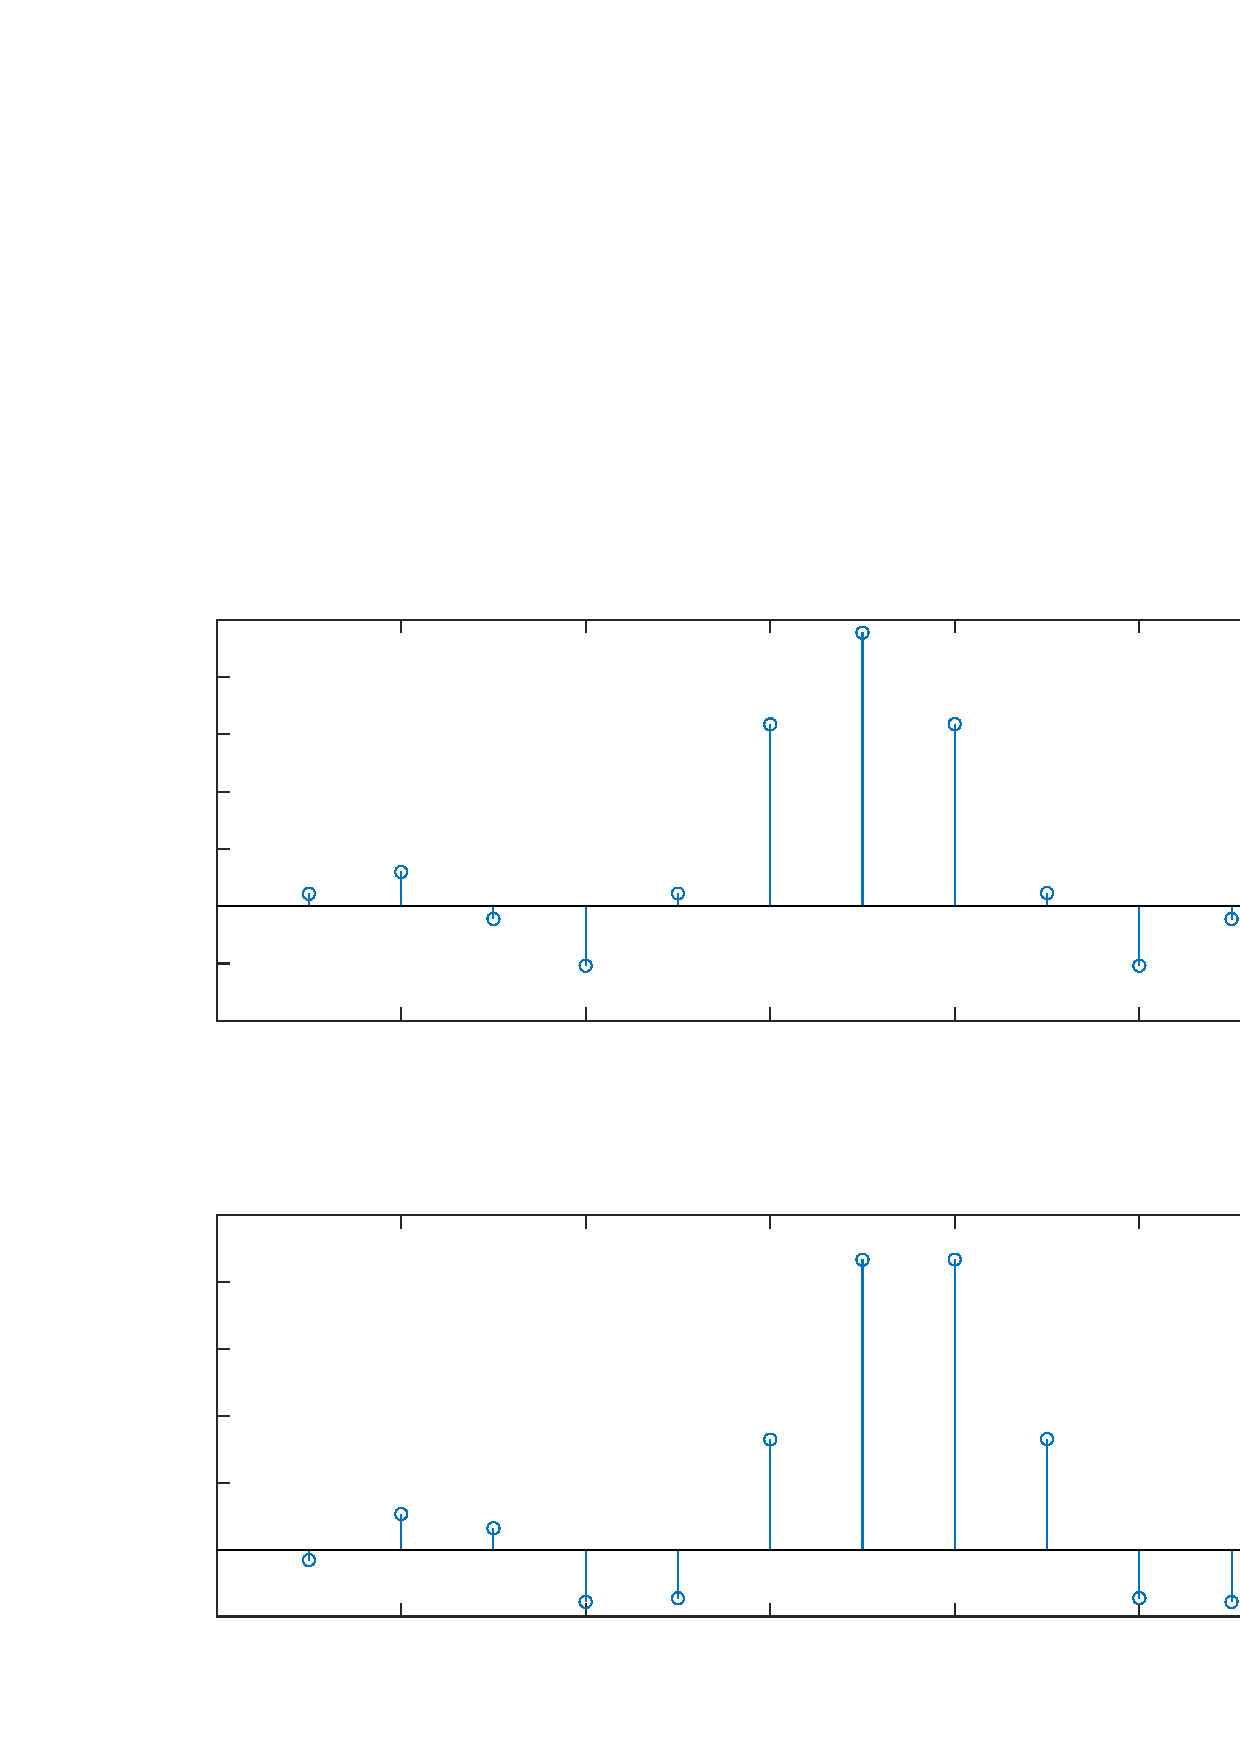
\includegraphics[scale=1]{octaves/linearPhaseTransferFunctionSinc-inc}
\end{picture}%
\begin{picture}(800,600)(0,0)
\fontsize{13}{0}\selectfont\put(104,341.514){\makebox(0,0)[t]{\textcolor[rgb]{0.15,0.15,0.15}{{0}}}}
\fontsize{13}{0}\selectfont\put(192.571,341.514){\makebox(0,0)[t]{\textcolor[rgb]{0.15,0.15,0.15}{{2}}}}
\fontsize{13}{0}\selectfont\put(281.143,341.514){\makebox(0,0)[t]{\textcolor[rgb]{0.15,0.15,0.15}{{4}}}}
\fontsize{13}{0}\selectfont\put(369.714,341.514){\makebox(0,0)[t]{\textcolor[rgb]{0.15,0.15,0.15}{{6}}}}
\fontsize{13}{0}\selectfont\put(458.286,341.514){\makebox(0,0)[t]{\textcolor[rgb]{0.15,0.15,0.15}{{8}}}}
\fontsize{13}{0}\selectfont\put(546.857,341.514){\makebox(0,0)[t]{\textcolor[rgb]{0.15,0.15,0.15}{{10}}}}
\fontsize{13}{0}\selectfont\put(635.429,341.514){\makebox(0,0)[t]{\textcolor[rgb]{0.15,0.15,0.15}{{12}}}}
\fontsize{13}{0}\selectfont\put(724,341.514){\makebox(0,0)[t]{\textcolor[rgb]{0.15,0.15,0.15}{{14}}}}
\fontsize{13}{0}\selectfont\put(97.0647,351.944){\makebox(0,0)[r]{\textcolor[rgb]{0.15,0.15,0.15}{{-0.2}}}}
\fontsize{13}{0}\selectfont\put(97.0647,379.444){\makebox(0,0)[r]{\textcolor[rgb]{0.15,0.15,0.15}{{-0.1}}}}
\fontsize{13}{0}\selectfont\put(97.0647,406.944){\makebox(0,0)[r]{\textcolor[rgb]{0.15,0.15,0.15}{{0}}}}
\fontsize{13}{0}\selectfont\put(97.0647,434.444){\makebox(0,0)[r]{\textcolor[rgb]{0.15,0.15,0.15}{{0.1}}}}
\fontsize{13}{0}\selectfont\put(97.0647,461.944){\makebox(0,0)[r]{\textcolor[rgb]{0.15,0.15,0.15}{{0.2}}}}
\fontsize{13}{0}\selectfont\put(97.0647,489.444){\makebox(0,0)[r]{\textcolor[rgb]{0.15,0.15,0.15}{{0.3}}}}
\fontsize{13}{0}\selectfont\put(97.0647,516.944){\makebox(0,0)[r]{\textcolor[rgb]{0.15,0.15,0.15}{{0.4}}}}
\fontsize{13}{0}\selectfont\put(97.0647,544.444){\makebox(0,0)[r]{\textcolor[rgb]{0.15,0.15,0.15}{{0.5}}}}
\fontsize{15}{0}\selectfont\put(414,554.444){\makebox(0,0)[b]{\textcolor[rgb]{0,0,0}{{N = 12}}}}
\fontsize{13}{0}\selectfont\put(104,55.5699){\makebox(0,0)[t]{\textcolor[rgb]{0.15,0.15,0.15}{{0}}}}
\fontsize{13}{0}\selectfont\put(192.571,55.5699){\makebox(0,0)[t]{\textcolor[rgb]{0.15,0.15,0.15}{{2}}}}
\fontsize{13}{0}\selectfont\put(281.143,55.5699){\makebox(0,0)[t]{\textcolor[rgb]{0.15,0.15,0.15}{{4}}}}
\fontsize{13}{0}\selectfont\put(369.714,55.5699){\makebox(0,0)[t]{\textcolor[rgb]{0.15,0.15,0.15}{{6}}}}
\fontsize{13}{0}\selectfont\put(458.286,55.5699){\makebox(0,0)[t]{\textcolor[rgb]{0.15,0.15,0.15}{{8}}}}
\fontsize{13}{0}\selectfont\put(546.857,55.5699){\makebox(0,0)[t]{\textcolor[rgb]{0.15,0.15,0.15}{{10}}}}
\fontsize{13}{0}\selectfont\put(635.429,55.5699){\makebox(0,0)[t]{\textcolor[rgb]{0.15,0.15,0.15}{{12}}}}
\fontsize{13}{0}\selectfont\put(724,55.5699){\makebox(0,0)[t]{\textcolor[rgb]{0.15,0.15,0.15}{{14}}}}
\fontsize{13}{0}\selectfont\put(97.0647,66){\makebox(0,0)[r]{\textcolor[rgb]{0.15,0.15,0.15}{{-0.1}}}}
\fontsize{13}{0}\selectfont\put(97.0647,98.0833){\makebox(0,0)[r]{\textcolor[rgb]{0.15,0.15,0.15}{{0}}}}
\fontsize{13}{0}\selectfont\put(97.0647,130.167){\makebox(0,0)[r]{\textcolor[rgb]{0.15,0.15,0.15}{{0.1}}}}
\fontsize{13}{0}\selectfont\put(97.0647,162.25){\makebox(0,0)[r]{\textcolor[rgb]{0.15,0.15,0.15}{{0.2}}}}
\fontsize{13}{0}\selectfont\put(97.0647,194.333){\makebox(0,0)[r]{\textcolor[rgb]{0.15,0.15,0.15}{{0.3}}}}
\fontsize{13}{0}\selectfont\put(97.0647,226.417){\makebox(0,0)[r]{\textcolor[rgb]{0.15,0.15,0.15}{{0.4}}}}
\fontsize{13}{0}\selectfont\put(97.0647,258.5){\makebox(0,0)[r]{\textcolor[rgb]{0.15,0.15,0.15}{{0.5}}}}
\fontsize{15}{0}\selectfont\put(414,268.5){\makebox(0,0)[b]{\textcolor[rgb]{0,0,0}{{N = 13}}}}
\end{picture}

}\caption{Stem plot of impulse response $\hat{h}_{LP}[n]$ for values $N = 12$ and $N = 13$. Notably, both are symmetric, and only the impulse response having an even $N$ value will possess a single, central peak.}\label{oct:linearPhaseTransferFunctionSinc}
\end{center}
\end{figure*}

Because of the symmetry of the impulse response coefficients as indicated in Figure~\ref{oct:linearPhaseTransferFunctionSinc}, the frequency response of the truncated approximation can be expressed as follows,
\[
    \hat{H}_{LP}(e^{j\omega}) = \sum_{n=0}^N \hat{h}_{LP}[n] e^{-j\omega n} = e^{-j\omega \frac N 2}\tilde{H}_{LP}(\omega),
\]
where $\tilde{H}_{LP}(\omega)$ is the \textbf{amplitude response}, a real function of $\omega$.

\subsection{Minimum phase and Maximum phase transfer functions}

Let $H_1(z)$ and $H_2(z)$ be two first-order transfer functions
\begin{align*}
    H_1(z) &= \frac{z+b}{z+a},\\
    H_2(z) &= \frac{bz+1}{z+a},
\end{align*}
for $|a|<1, |b| < 1$. Both transfer functions have a pole inside the unit circle (which is $z=-a$) and are thus \emph{stable}. However, they differ for their zeros: the zero of the first lies inside the unit circle $z=-b$, while the zero of the second is outside of the unit circle, $z=-\frac 1 b$, situated in a mirror image symmetry fashion. Figure~\ref{tikz:minimumMaximumPhaseTransferFunctionsPlot} shows a plot of zeros and poles of both functions.

\begin{figure*}
\begin{center}
    \begin{tikzpicture}
        \draw[thick,-stealth] (-2.5,0) -- (2.5,0) node[anchor=north west] {$\Re z$};
        \draw[thick,-stealth] (0,-2.5) -- (0,2.5) node[anchor=south east] {$\Im z$};
        \draw (1pt, 1.5) -- (-1pt, 1.5) node[anchor=south west] {$1$};
        \node[draw, circle, thick, minimum size=3cm] at (0,0) {};
        \node[draw, polez, thick, label=south:{$-a$}] at (-.8, 0) {};
        \node[draw, zeroz, thick, label=south:{$-b$}] at (1.2, 0) {};
        \node at (2,2) {$H_1(z)$};
    \end{tikzpicture}
    \begin{tikzpicture}
        \draw[thick,-stealth] (-2.5,0) -- (2.5,0) node[anchor=north west] {$\Re z$};
        \draw[thick,-stealth] (0,-2.5) -- (0,2.5) node[anchor=south east] {$\Im z$};
        \draw (1pt, 1.5) -- (-1pt, 1.5) node[anchor=south west] {$1$};
        \node[draw, circle, thick, minimum size=3cm] at (0,0) {};
        \node[draw, polez, thick, label=south:{$-a$}] at (-.8, 0) {};
        \node[draw, zeroz, thick, label=south:{$-\frac 1 b$}] at (1.8, 0) {};
        \node at (2,2) {$H_2(z)$};
    \end{tikzpicture}
\end{center}\caption{Zero-poles plot of transfer functions $H_1(z)$ and $H_2(z)$. Zero at $z = -\frac 1 b$ is the mirror-image zero of $z=-b$.}\label{tikz:minimumMaximumPhaseTransferFunctionsPlot}
\end{figure*}

However, both transfer functions have an identical magnitude function, as the following equality holds,
\[
    H_1(z)H_1(z^{-1}) = H_2(z)H_2(z^{-1})
\]
with the phase functions
\begin{align*}
    \arg{H_1(e^{j\omega})} &= \tan^{-1}\frac{\sin \omega}{b + \cos \omega} - \tan^{-1} \frac{\sin \omega}{a + \cos \omega},\\
    \arg{H_2(e^{j\omega})} &= \tan^{-1}\frac{b\sin \omega}{1 + b\cos \omega} - \tan^{-1} \frac{\sin \omega}{a + \cos \omega}.
\end{align*}

\begin{figure*}[ht]
\begin{center}
\scalebox{0.45}{
    % Title: Figure 1
% Creator: GL2PS 1.4.2, (C) 1999-2020 C. Geuzaine
% For: Octave
% CreationDate: Mon Dec 19 15:50:53 2022
\setlength{\unitlength}{1pt}
\begin{picture}(0,0)
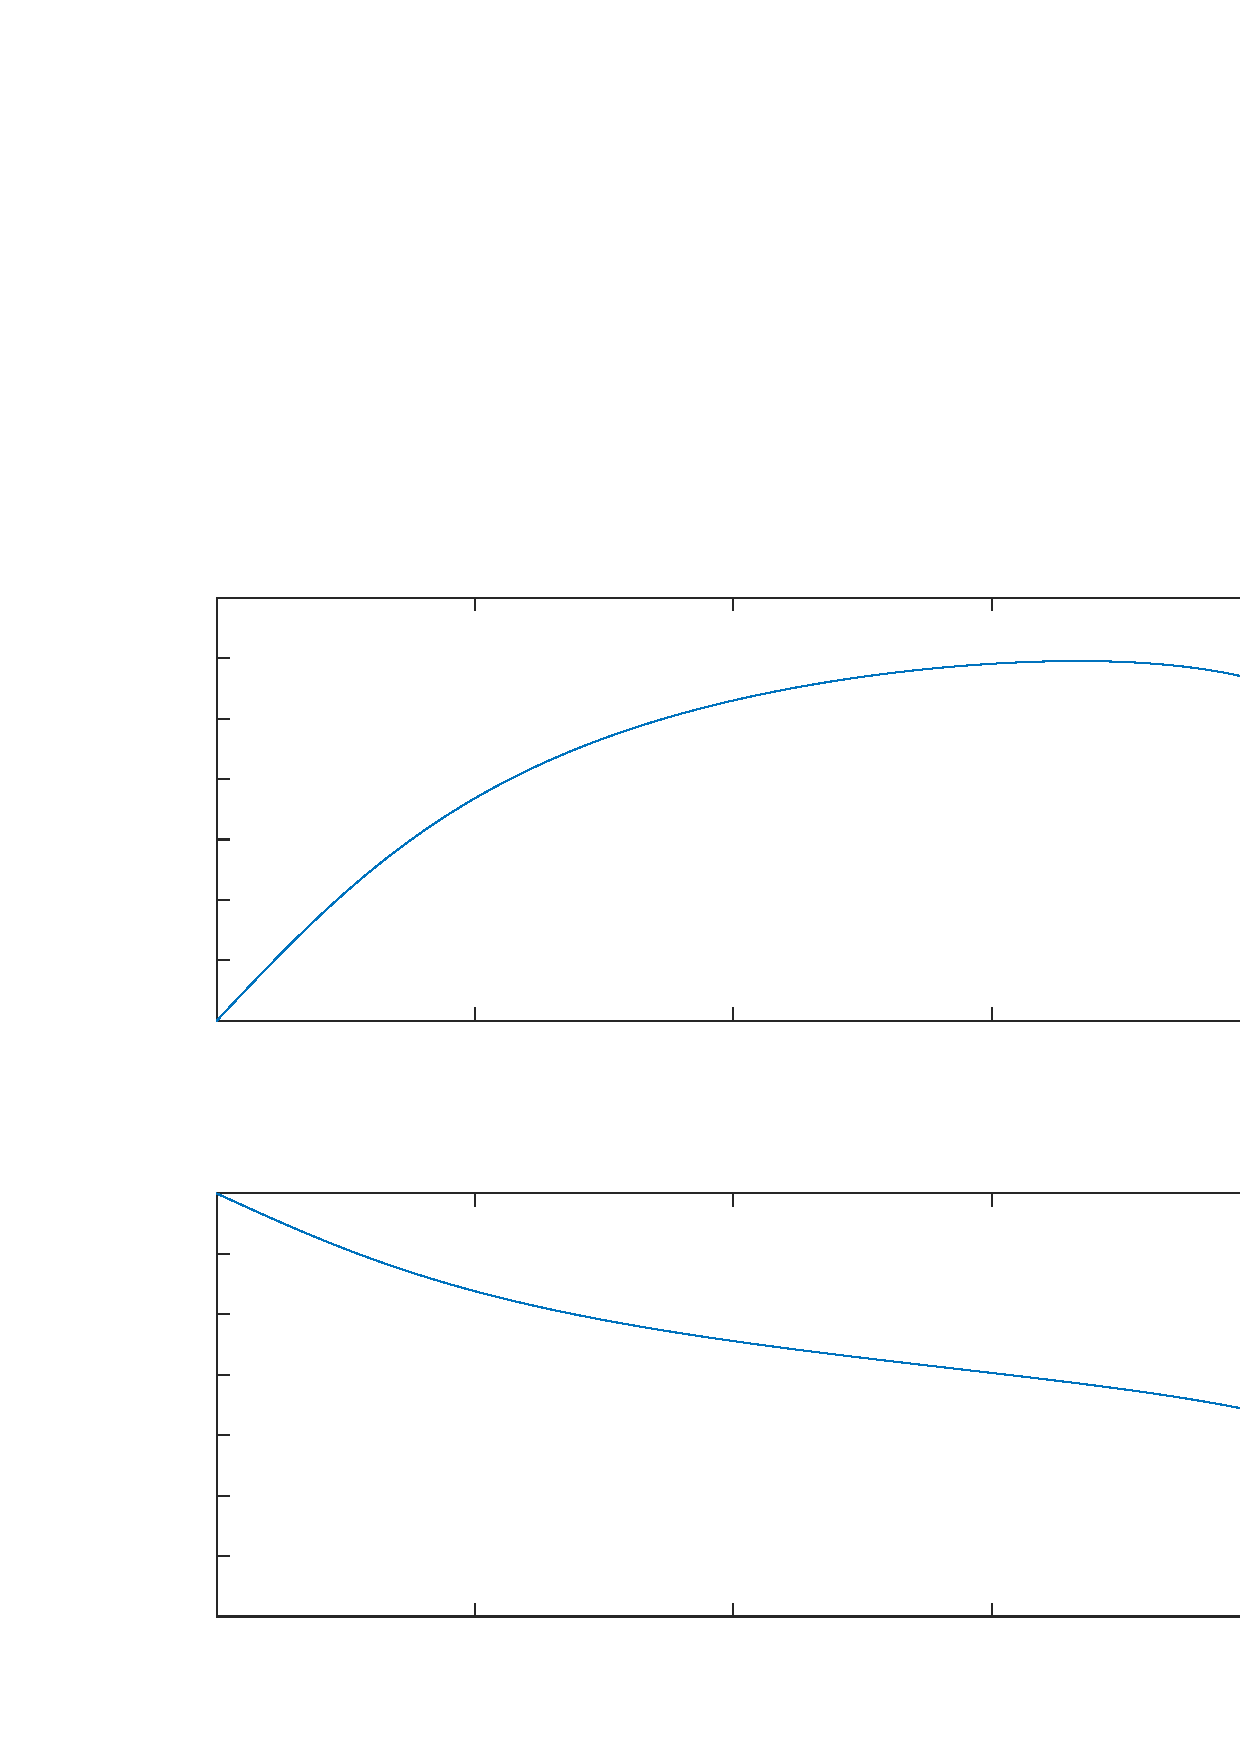
\includegraphics[scale=1]{octaves/minimumPhaseMaximumPhaseExamplePhase-inc}
\end{picture}%
\begin{picture}(800,600)(0,0)
\fontsize{13}{0}\selectfont\put(104,341.538){\makebox(0,0)[t]{\textcolor[rgb]{0.15,0.15,0.15}{{0}}}}
\fontsize{13}{0}\selectfont\put(228,341.538){\makebox(0,0)[t]{\textcolor[rgb]{0.15,0.15,0.15}{{0.2}}}}
\fontsize{13}{0}\selectfont\put(352,341.538){\makebox(0,0)[t]{\textcolor[rgb]{0.15,0.15,0.15}{{0.4}}}}
\fontsize{13}{0}\selectfont\put(476,341.538){\makebox(0,0)[t]{\textcolor[rgb]{0.15,0.15,0.15}{{0.6}}}}
\fontsize{13}{0}\selectfont\put(600,341.538){\makebox(0,0)[t]{\textcolor[rgb]{0.15,0.15,0.15}{{0.8}}}}
\fontsize{13}{0}\selectfont\put(724,341.538){\makebox(0,0)[t]{\textcolor[rgb]{0.15,0.15,0.15}{{1}}}}
\fontsize{13}{0}\selectfont\put(97.0647,351.944){\makebox(0,0)[r]{\textcolor[rgb]{0.15,0.15,0.15}{{0}}}}
\fontsize{13}{0}\selectfont\put(97.0647,380.952){\makebox(0,0)[r]{\textcolor[rgb]{0.15,0.15,0.15}{{0.2}}}}
\fontsize{13}{0}\selectfont\put(97.0647,409.96){\makebox(0,0)[r]{\textcolor[rgb]{0.15,0.15,0.15}{{0.4}}}}
\fontsize{13}{0}\selectfont\put(97.0647,438.968){\makebox(0,0)[r]{\textcolor[rgb]{0.15,0.15,0.15}{{0.6}}}}
\fontsize{13}{0}\selectfont\put(97.0647,467.976){\makebox(0,0)[r]{\textcolor[rgb]{0.15,0.15,0.15}{{0.8}}}}
\fontsize{13}{0}\selectfont\put(97.0647,496.984){\makebox(0,0)[r]{\textcolor[rgb]{0.15,0.15,0.15}{{1}}}}
\fontsize{13}{0}\selectfont\put(97.0647,525.992){\makebox(0,0)[r]{\textcolor[rgb]{0.15,0.15,0.15}{{1.2}}}}
\fontsize{13}{0}\selectfont\put(97.0647,555){\makebox(0,0)[r]{\textcolor[rgb]{0.15,0.15,0.15}{{1.4}}}}
\fontsize{13}{0}\selectfont\put(104,55.5941){\makebox(0,0)[t]{\textcolor[rgb]{0.15,0.15,0.15}{{0}}}}
\fontsize{13}{0}\selectfont\put(228,55.5941){\makebox(0,0)[t]{\textcolor[rgb]{0.15,0.15,0.15}{{0.2}}}}
\fontsize{13}{0}\selectfont\put(352,55.5941){\makebox(0,0)[t]{\textcolor[rgb]{0.15,0.15,0.15}{{0.4}}}}
\fontsize{13}{0}\selectfont\put(476,55.5941){\makebox(0,0)[t]{\textcolor[rgb]{0.15,0.15,0.15}{{0.6}}}}
\fontsize{13}{0}\selectfont\put(600,55.5941){\makebox(0,0)[t]{\textcolor[rgb]{0.15,0.15,0.15}{{0.8}}}}
\fontsize{13}{0}\selectfont\put(724,55.5941){\makebox(0,0)[t]{\textcolor[rgb]{0.15,0.15,0.15}{{1}}}}
\fontsize{13}{0}\selectfont\put(97.0647,66){\makebox(0,0)[r]{\textcolor[rgb]{0.15,0.15,0.15}{{-3.5}}}}
\fontsize{13}{0}\selectfont\put(97.0647,95.008){\makebox(0,0)[r]{\textcolor[rgb]{0.15,0.15,0.15}{{-3}}}}
\fontsize{13}{0}\selectfont\put(97.0647,124.016){\makebox(0,0)[r]{\textcolor[rgb]{0.15,0.15,0.15}{{-2.5}}}}
\fontsize{13}{0}\selectfont\put(97.0647,153.024){\makebox(0,0)[r]{\textcolor[rgb]{0.15,0.15,0.15}{{-2}}}}
\fontsize{13}{0}\selectfont\put(97.0647,182.032){\makebox(0,0)[r]{\textcolor[rgb]{0.15,0.15,0.15}{{-1.5}}}}
\fontsize{13}{0}\selectfont\put(97.0647,211.04){\makebox(0,0)[r]{\textcolor[rgb]{0.15,0.15,0.15}{{-1}}}}
\fontsize{13}{0}\selectfont\put(97.0647,240.048){\makebox(0,0)[r]{\textcolor[rgb]{0.15,0.15,0.15}{{-0.5}}}}
\fontsize{13}{0}\selectfont\put(97.0647,269.056){\makebox(0,0)[r]{\textcolor[rgb]{0.15,0.15,0.15}{{0}}}}
\end{picture}

}\caption{Unwrapped phase responses of transfer functions $H_1(z)$ and $H_2(z)$ for values of $a = 0.8$ and $b = -0.5$.}\label{oct:minimumPhaseMaximumPhaseExamplePhase}
\end{center}
\end{figure*}

Figure~\ref{oct:minimumPhaseMaximumPhaseExamplePhase} shows off that $H_2(z)$ has an \emph{excess phase lag} with respect to $H_1(z)$---the excess phase lag of $H_2(z)$ is caused by its very nature, in fact
\[
    H_2(z) = \frac{bz + 1}{z + a} = \underbrace{\left(\frac{z + b}{z + a}\right)}_{H_1(z)}\underbrace{\left(\frac{bz + 1}{z + b}\right)}_{A(z)},
\]
where $A(z) = \frac{bz + 1}{z + b}$ is a \emph{stable allpass function} which basically introduces a phase group delay which is proportional to the order of the allpass filter. (In this peculiar case, the order of the allpass filter is $M=1$, so for Equation~\ref{eqn:allpassIntegralPhaseEquation} a phase delay of $M\pi = \pi$ will be introduced.) Indeed, the phase function of $H_2(z)$ will be the sum of the phase functions of both above terms,
\[
    \arg{H_2(e^{j\omega})} = \arg{H_1(e^{j\omega})} + \arg{A(e^{j\omega})};
\]
as the unwrapped phase function of a stable first-order allpass function is a negative function in $\omega$, it follows from the above that $H_2(z)$ has an \textbf{excess phase lag} with respect to its ``twin'' filter $H_1(z)$.

To generalize, let $H_m(z)$ be a causal stable transfer function with all zeros inside the unit circle, and let $H(z)$ be any causal stable transfer function with the same magnitude
\[
    \left|H(e^{j\omega})\right| = \left|H_m(e^{j\omega})\right|.
\]
The two transfer functions can be put in relation through the following equation,
\begin{equation}\label{eqn:minimumPhaseMaximumPhaseRelation}
    H(z) = H_m(z)A(z)
\end{equation}
where $A(z)$ is an \emph{allpass function} which is causal and stable. Their magnitude is the same, however, regarding its phase,
\begin{equation}\label{eqn:minimumPhaseMaximumPhaseExcessPhase}
    \arg{H(e^{j\omega})} = \arg{H_m(e^{j\omega})} + \arg{A(e^{j\omega})}
\end{equation}
the transfer function $H(z)$ it is said to have an \textbf{excess phase lag} with respect to $H_m(z)$---the latter is called a \textbf{minimum-phase transfer function}.

Essentially, a transfer function whose zeros are all inside the unit circle $H_m(z)$ is said to possess a \emph{minimum-phase delay}. Intrinsically, any other transfer function $H(z)$ whose magnitude is the same of $H_m(z)$ can be always re\"expressed by the product of $H_m(z)$ \emph{and} a specially crafted allpass function $A(z)$. Since the allpass function will introduce a phase group delay of $\pi$ \emph{for each} pole $M$, the transfer function $H(z)$ will exhibit a \emph{greater} amount of phase delay when put in comparison with $H_m(z)$, unless the allpass filter has no poles---but this suggests that the allpass filter is a $0$th-order filter; a filter with no poles at all. This circumstance, however, occurs only if the transfer function has \emph{all zeros inside the unit circle}. It is enough for it to have at least a zero outside the unit circle, that the allpass filter $A(z)$ will exhibit at least a pole---causing a non-zero phase group delay.

This leads to other two new definitions. The first one is the exact opposite of the former. Causal stable transfer functions will \emph{all zeros} outside the unit circle are said to be \textbf{maximum-phase transfer functions}---consonantly, causal stable transfer functions with zeros both inside and outside the unit circle are called \textbf{mixed-phase transfer functions}. Both ones will present an excess of phase lag with respect to another minimum-phase transfer function $H_m(z)$.

An example of this could be the following mixed-phase transfer function,
\[
    H(z) = \frac{
        2(1 + 0.3z^{-1})(0.4 - z^{-1})
    } {
        (1-0.2z^{-1})(1 + 0.5z^{-1})
    }
\]
which exhibits a zero outside the unit circle ($z = 2.5$).

Thanks to Equation~\ref{eqn:minimumPhaseMaximumPhaseRelation}, the transfer function can be re\"arranged into the following form
\[
    H(z) = \left[\frac{
        2(1+0.3z^{-1})(1-0.4z^{-1})
    } {
        (1-0.2z^{-1})(1+0.5z^{-1})
    }\right] \left( \frac{
        0.4 - z^{-1}
    } {
        1 - 0.4z^{-1}
    }\right),
\]
and---as expected---the allpass function in round brackets presents a pole, which alters the phase complexively of $\pi$. We have been able to re\"arrange the transfer function in a new form only because a zero outside of the unit circle was present. The rogue zero was embodied in the factor $(0.4 - z^{-1})$ at numerator, and is was sufficient to multiply--divide by the term $(1 - 0.4z^{-1})$ to automatically craft an allpass transfer function.

\clearpage

\chapter{Signal distortions, Oscillators}

\section{Inverse systems}
Signals $x[n]$ that pass through LTI systems over which the designer has no control (this includes those that can be expressed in the rational form $H(z) = \frac{B(z)}{A(z)}$) will generally be subject to a \textbf{distortion}---which may often be undesired. To remove it, various techniques exist: a first straightforward technique is to determine the so called \textbf{inverse system}, a system that, if applied to the distorted signal, it ``nullifies'' the distortion induced by the LTI system. Such a system will be denoted as $H^{-1}(z)$ and will possess a transfer function of form $H^{-1}(z) = \frac{A(z)}{B(z)}$---na\"ively, the reciprocal of the original LTI system's rational transfer function. Such a filter, if applied after the first one, will ideally cancel unwanted distortions induced by the former.

\begin{center}
    \begin{tikzpicture}
        \node at (0, 0)(x) {$x[n]$};
        \node[draw, thick, rectangle, minimum width=1.3cm, minimum height=.6cm](H) at (1.5, 0) {$H(z)$};
        \node at (2.75, .2)(w) {$w[n]$};
        \node[draw, thick, rectangle, minimum width=1.3cm, minimum height=.6cm](HI) at (4, 0) {$H^{-1}(z)$};
        \node at (5.5, 0)(tx) {$\tilde{x}[n]$};
        \draw[-stealth] (x) -- (H);
        \draw[-stealth] (H) -- (HI);
        \draw[-stealth] (HI) -- (tx);
    \end{tikzpicture}
\end{center}

The above system is constructed so that the desired behavior is 
\[
    \tilde{x}[n] \equiv x[n],
\]
so that the output signal $\tilde{x}[n]$ is the same of the input signal $x[n]$ before it passed through the LTI system $H(z)$ which induced undesired distortions---apart for a delay which is induced by the system as a whole.

It must be pointed out that the inverse system is completely determined only if its Region of Convergence is also defined. Typically, one wants \emph{causal} inverse systems, but sometimes it might be useful---for instance for applications which do not require real-time processing---to obtain a ROC which is typical of a non-causal inverse system.

Let $H_e(z)$ be an example transfer function
\[
    H_e(z) = \frac{
        (z - \frac 1 4)(z + \frac 1 5)
    } {
        (z + \frac 1 2)(z - \frac 1 3)
    },
\]
its inverse system is quickly ascertainable by replacing the numerator with the denominator, and vice-versa,
\[
    H_e^{-1}(z) = \frac{
        (z + \frac 1 2)(z - \frac 1 3)
    } {
        (z - \frac 1 4)(z + \frac 1 5)
    }.
\]

The inverse system will have a different Region of Convergence than the original system---indeed, three cases are possible:
\begin{itemize}
    \item the first is $|z| > \frac 1 4$---a causal, stable region;
    \item the second is $|z| < \frac 1 5$---an anticausal, unstable region;
    \item the third and last is $\frac 1 5 < |z| < \frac 1 4$---bilateral, unstable.
\end{itemize}

In general, there is no guarantee that the inverse system technique will produce a useful result. The inverse system technique, in fact, requires the knowledge of the LTI system $H(z)$ first to determine its inverse system. Very much, it is really unlikely that the designer will know the nature of the LTI system $H(z)$; more frequently, the exact formula of $H(z)$ will be completely unknown. Secondarily, there will always be some kind of noise disturbing the signal. Under an excess of noise, it is truly difficult---let alone possible---to ascertain the nature of $H(z)$. The noise occurs as an additive signal $d[n]$ to the intermediate signal $w[n]$. Ultimately, quantization will make the process of determining the inverse system even harder, as errors in computation prevent the design of an \emph{exact} inverse system's filter.

For a causal system $H(z)$, its inverse system $H^{-1}(z)$ can only be built if the former is a \textbf{minimum phase} system: all poles and zeros exchange their position moving from $H$ to $H^{-1}$ (its numerator takes the place of the denominator, and vice-versa), hence all zeros outside the unit circle would be come poles outside the unit circle, which would clearly render the inverse system unstable.

The inverse system procedure has its own advantages and disadvantages. First and foremost, it is \emph{simple to understand}---ideally, an inverse system is just a system defined as the reciprocal of the transfer function of another system. Any distortion induced by the latter can be ``corrected'' with the application of the inverse system, with the only byproduct being the \emph{introduction of a delay}, which could be a disadvantage or not. However, in order to adopt such technique, \emph{the original direct system $H(z)$ must be well-known}; a feat that rarely and hardly occurs. Moreover, \emph{additive noise} could boycott the functioning of the inverse system, as well as \emph{quantization errors}. In practice, it is very hard to employ this simple technique effectively, due to the underlying issues that inevitably affect it.

\section{Recursive deconvolution}

\textbf{Recursive deconvolution} is a technique that allows to recover a signal $x[n]$ by means of an \emph{estimation} $\bar{x}[n]$ directly in the time domain. In order to produce such an estimation, the impulse response $h[n]$ of the truncated IIR (that is, a FIR response) of the system must be known in advance.

Let $x[n]$ be a causal sequence, then it is true that
\[
    \bar{x}[n] = \sum_{k=0}^n x[k]h[n-k].
\]

Now, let's determine some of its values:
\begin{align*}
    \bar{x}[0] &= x[0]h[0] \longrightarrow x[0] = \frac{\bar{x}[0]}{h[0]}\\
    \bar{x}[1] &= x[0]h[1] + x[1]h[0] \longrightarrow x[1] = \frac{\bar{x}[1] - x[0]h[1]}{h[0]}\\
    \bar{x}[2] &\longrightarrow x[2] = \frac{\bar{x}[2] - x[1]h[1] - x[0]h[2]}{h[0]}\\
    \vdots \hspace{.3cm}     &= \hspace{2cm} \vdots\\
    \bar{x}[n] &= x[n]h[0] + \sum_{k=0}^{n-1}x[k]h[n-k]\\ 
    \longrightarrow & x[n] = \frac{\bar{x}[n] - \sum_{k=0}^{n-1}x[k]h[n-k]}{h[0]}.\\
\end{align*}

This way, it is possible to retrieve a signal $x[n]$ from its estimate $\bar{x}[n]$, provided $h[n]$ is known in advance. The main disadvantages of this technique are that $h$ should be predetermined, and secondly that the process can accumulate errors, as errors at any sample will propagate recursively, since to determine $x[\kappa]$ it is necessary to have priorly determined $x[\kappa - 1]$ (and all previous samples as well, of course, starting from $x[0]$). This method provides a clever way to obtain a sequence $x[n]$ from an estimation of it, directly in the time domain; however, one should be careful in the design, as any error can propagate and sum altogether.

\section{Sinusoidal digital oscillators}

Crucially important devices in electronics and signal processing are the \textbf{sinusoidal oscillators}. Sinusoidal oscillators are special filters, either analog or digital, that after being activated by a \emph{trigger} are capable of producing an \emph{oscillation} of values, at a certain frequency $\omega_0$, indefinitely in time. In digital signal processing, the digital version of the sinusoidal oscillators are the \textbf{sinusoidal digital oscillators}.

\begin{defin}[Sinusoidal digital oscillator]
    A \textbf{sinusoidal digital oscillator} with oscillation frequency $\omega_0$ is any device whose transfer function has the form
    \begin{eqnarray}\label{eqn:sinusoidalDigitalOscillator}
        H_{\omega_0}(z) &= \frac{
            1
        } {
            (1 - pz^{-1})(1 - p^*z^{-1})
        } = \frac {
            1
        } {
            1 - (p + p^*)z^{-1} + pp^*z^{-2}
        }\\ &= \frac {
            1
        } {
            1 - 2\cos{(\omega_0)} z^{-1} + z^{-2}
        },
    \end{eqnarray}
    with $p$ and $p^*$ the pair of \emph{complex--conjugate poles} located in the unit circle, and $p = e^{j\omega_0}$, $|p| = 1$. In time domain, the formula is
    \begin{equation}\label{eqn:sinusoidalDigitalOscillatorTime}
        y[n] = x[n] + 2\cos{(\omega_0)}y[n-1] - y[n-2].
    \end{equation}
    Before sample $0$, an oscillator has output equal to zero, hence $y[-1]=y[-2]=0$.

    The \textbf{trigger} for the sinusoidal digital oscillator is the input sequence
\begin{equation}\label{eqn:sinusoidalDigitalOscillatorTrigger}
    x_T[n] = A\sin{(\omega_0)}\delta[n].
\end{equation}
    A trigger sequence will initialize the oscillator, causing it to produce the sinusoidal output sequence indefinitely.
\end{defin}

Let an oscillator be as described by Equation~\ref{eqn:sinusoidalDigitalOscillator} and let the trigger input sequence be the one introduced in Equation~\ref{eqn:sinusoidalDigitalOscillatorTrigger}; then, the resulting output sequence will be
\[
    y[n] = \{A\sin\omega_0, 2A\sin\omega_0\cos\omega_0 = A\sin{2\omega_0}, A\sin{3\omega_0}, \dots, A\sin{n\omega_0}\}.
\]

Suitable initial conditions allow to discard the trigger input $x[n]$ altogether,
\begin{equation}\label{eqn:sinusoidalDigitalOscillatorTriggerInitialConditionsFormula}
    y[n] = 2\cos{(\omega_0)}y[n-1] - y[n-2],
\end{equation}
with peculiar initial conditions
\begin{align}\label{eqn:sinusoidalDigitalOscillatorTriggerInitialConditions}
    y[-1] &= 0,\\
    y[-2] &= -A\sin{\omega_0}.
\end{align}


\chapter{Linear phase FIR transfer functions}
In Section~\ref{sec:linearPhaseTransferFunctions} we briefly investigated some properties of the linear phase transfer functions. To summarize, linear phase transfer functions are all those transfer functions which present a \emph{linear} phase characteristic in a determined frequency range---called band of interest---and whose formula is
\[
    H(e^{j\omega}) = e^{-j\omega D},
\]
with $D\in\R$. Other properties were that $\left|e^{-j\omega D}\right| = 1$ and that the group delay was completely constant along the way from $0$ to $2\pi$,
\[
    \tau(\omega) = D.
\]

We have also seen that the output $y[n]$ of a linear phase filter to the specially crafted input $x[n]=Ae^{j\omega n}$ is
\[
    y[n] = Ae^{j\omega D} e^{j\omega n} = Ae^{j\omega(n - D)}.
\]


When dealing with digital signals, the nature of $D$ matters: if $D$ is not an integer, the outcome of a linear phase transfer function will be dissimilar to the input. Conversely, linear phase systems with integer $D$s will produce an outcome which is similar to the input, but delayed of $D\in\Z$ samples.

In general, it is impossible to design an IIR transfer function with an exact linear phase. However, for a limited band of interest and for FIR transfer functions, it is \emph{always possible} to design a linear phase transfer function, for instance by truncating a sinc-shaped impulse response. To recall, the IIR impulse response, of linear phase,
\[
    h_{IIR,lp}[n] = \frac{
        \sin{(\omega_c(n - n_0))}
    } {
        \pi (n - n_0)
    }, -\infty < n < \infty.
\]
can be truncated to the FIR impulse response, of linear phase as well,
\[
    \hat{h}_{FIR,lp}[n] = \frac{
        \sin{(\omega_c(n - \frac N 2))}
    } {
        \pi (n - \frac N 2)
    }, 0 \leq n \leq N,
\]
an impulse response of length $N+1$, which is both causal and of linear phase. Such a \emph{sinc} impulse will have its center on sample $\frac N 2$; in the case of even $N$, it would be in the middle between the two samples located at the center.

We will now develop the forms of the linear phase FIR transfer function $H(z)$ from a real impulse response $h[n]$.

Let
\[
    H(z) = \sum_{n=0}^N h[n]z^{-n};
\]
if $H(z)$ should have a linear phase response, its frequency response must have the following form,
\begin{equation}\label{eqn:linearPhaseTransferFunctionForm}
    H(e^{j\omega}) = e^{j(c\omega + \beta)}\breve{H}(\omega),
\end{equation}
where $c$ and $\beta$ are constants and $\breve{H}(\omega)$ is said to be the \textbf{amplitude response} or \textbf{zero phase response}. From now on, we can always write linear phase systems as the product of two terms, the first one being a term which is only responsible for producing a shift in phase---a \emph{linear} shift, in this case. This term will not contribute to the amplitude of the linear phase transfer function in any way. The second term, on contrary, has the sole purpose of being responsible of the amplitude of the filter---with \emph{no} contribution to phase. As such, the amplitude response is a real function in $\omega$. Its nature also depends on the nature of $H(z)$: if the latter is a real transfer function, then the amplitude response will be an \emph{even} function (this means that $\left|H(e^{j\omega})\right| = \left|H(e^{-j\omega})\right|$). Not only that---since $\left|H(e^{j\omega})\right| = \left|\breve{H}(\omega)\right|$, the amplitude response is \emph{either} an even or an odd function in $\omega$, that means that
\[
    \breve{H}(-\omega) = \pm\breve{H}(\omega).
\]

As any transfer function follows the property
\begin{equation}\label{eqn:transferFunctionSymmetryProperty}
    H(e^{j\omega}) = H^*(e^{-j\omega})
\end{equation}
a linear phase transfer function must abide to it as well. For linear phase transfer functions the above can be rewritten into
\[
    e^{j(c\omega + \beta)}\breve{H}(\omega) = e^{-j(c\omega + \beta)}\breve{H}(-\omega).
\]
Two fundamental cases must be distinguished then: the case of an \textbf{even} $\breve{H}(\omega)$ and the case of an \textbf{odd} $\breve{H}(\omega)$.

In the case that $\breve{H}(\omega)$ is an even function in $\omega$, then $\breve{H}(-\omega) = \breve{H}(+\omega)$ and the above becomes
\[
    e^{j\beta} = e^{-j\beta}
\]
implying that either $\beta = 0$ or $\beta = \pi$. Following up, from Equation~\ref{eqn:linearPhaseTransferFunctionForm} one can express the amplitude response in terms of the inverse transform
\begin{align*}
    \breve{H}(\omega) &= e^{-j(c\omega + \beta)}H(e^{j\omega})\\
                      &= e^{-j\beta}\sum_{n=0}^N h[n]e^{-j\omega(c + n)}.
\end{align*}
Since the amplitude function is even, we could freely replace $\omega$ with $-\omega$; however, for the moment let's only determine $\breve{H}(-\omega)$,
\[
    \breve{H}(-\omega) = e^{-j\beta}\sum_{l=0}^N h[l]e^{+j\omega(c + l)},
\]
at it can be determined in an analogous way as the previous one.
Making change of variable $l = N - n$, one can rewrite the above as
\[
    \breve{H}(-\omega) = e^{-j\beta}\sum_{n=0}^N h[N - n]e^{j\omega(c + N - n)}.
\]
Now we can make use of the even nature of the amplitude response---as $\breve{H}(-\omega) = \breve{H}(+\omega)$, it is possible to equate the above formulas into
\[
    h[n]e^{-j\omega(c+n)} = h[N-n]e^{j\omega(c + N - n)};
\]
by choosing $c = -\frac N 2$, one has, for left and right sides,
\begin{align*}
    h[n]e^{-j\omega(-\frac N 2 + n)} &= h[n]e^{+j\omega(+\frac N 2 - n)}\\
    h[N - n]e^{j\omega(-\frac N 2 + N - n)} &= h[N - n]e^{+j\omega(+\frac N 2 - n)}
\end{align*}
with the first equation resulting from the left side of the previous condition, and the second equation resulting from the right side of the condition. Equating them yields
\[
    h[n] = h[N-n], 0 \leq n \leq N.
\]

This result clearly shows that, for \emph{even} amplitude functions, \textbf{the impulse response is symmetric}---or, equivalently, a FIR filter with an \emph{even} amplitude response can have a linear phase response only if it has a \textbf{symmetric impulse response}. Since property in Equation~\ref{eqn:transferFunctionSymmetryProperty} is true for all transfer functions, above condition is the same as equaling
\[
    e^{j(c\omega + \beta)}\breve{H}(\omega) = e^{-j(-c\omega + \beta)}\breve{H}(-\omega).
\]

We have just seen what happens when the amplitude function is an even function of $\omega$---what would happen in the case of an \textbf{odd} function?

An odd amplitude function would satisfy
\[
    \breve{H}(\omega) = -\breve{H}(-\omega),
\]
and, essentially, this means that from the equation
\[
    e^{j(c\omega + \beta)}\breve{H}(\omega) = e^{-j(-c\omega + \beta)}\breve{H}(-\omega).
\]
we get
\[
    e^{j\beta} = -e^{-j\beta},
\]
which can only be satisfied if $\beta = \frac \pi 2$ or $\beta = -\frac \pi 2$. Again, from~\ref{eqn:linearPhaseTransferFunctionForm}, one obtains
\begin{align*}
    \breve{H}(\omega) &= e^{-j(c\omega + \beta)}H(e^{j\omega})\\
                      &= e^{-j\beta}\sum_{n=0}^N h[n]e^{-j\omega(c + n)},
\end{align*}
just like before. From the above, inverting $\omega$ yields
\[
    \breve{H}(-\omega) = e^{-j\beta}\sum_{n=0}^N h[n]e^{+j\omega(c + n)},
\]
but this time $\breve{H}(\omega)$ is an odd function, and as such (by again replacing $l = N - n$)
\begin{align*}
    \breve{H}(-\omega) &= -\breve{H}(\omega) = -e^{-j\beta}\sum_{n=0}^N h[n]e^{-j\omega(c + n)}\\
                       &=  -e^{-j\beta}\sum_{n=0}^N h[N - n]e^{-j\omega(c + N - n)}
\end{align*}
Equating the obtained results yields
\[
    e^{-j\beta}\sum_{n=0}^N h[n]e^{+j\omega(c + n)} = -e^{-j\beta}\sum_{n=0}^N h[N - n]e^{-j\omega(c + N - n)}.
\]
For $c = -\frac N 2$, one gets
\[
    \sum_{n=0}^N h[n]e^{+j\omega(-\frac N 2 + n)} = -\sum_{n=0}^N h[N - n]e^{-j\omega(-\frac N 2 + N - n)},
\]
which leads to
\[
    \sum_{n=0}^N h[n]e^{-j\omega(\frac N 2 - n)} = -\sum_{n=0}^N h[N - n]e^{-j\omega(\frac N 2 - n)};
\]
but this ultimately provides
\[
    h[n] = -h[N-n], 0 \leq n \leq N.
\]

This last result, similarly to the previous one, can be interpreted with the fact that a FIR filter with an \emph{odd} amplitude response will have a linear phase response only if it has an \textbf{anti-symmetric impulse response}. Remember that, in order to retrieve the two results, the amplitude response had to be either even or odd---but one of the two conditions are always satisfied---and $c=-\frac N 2$. A linear phase transfer function will have $c$ always equal to $-\frac N 2$, and the value of $\beta$ either $0$,$2\pi$ or $\frac \pi 2$, $-\frac \pi 2$ depending depending---respectively---whether the amplitude response is even or odd.

Since the length of the impulse response is $N$, a number that can be either or odd, \emph{four} kinds of linear phase FIR transfer functions can be described,
\begin{enumerate}
    \item a FIR transfer function with symmetric impulse response, and with odd length;
    \item a FIR transfer function with symmetric impulse response, and with even length;
    \item a FIR transfer function with anti-symmetric impulse response, and with odd length;
    \item a FIR transfer function with anti-symmetric impulse response, and with even length.
\end{enumerate}

\section{Type 1: Symmetric impulse response with odd length and even $N$}

\begin{figure*}[ht]
\begin{center}
\scalebox{0.45}{
    % Title: Figure 1
% Creator: GL2PS 1.4.2, (C) 1999-2020 C. Geuzaine
% For: Octave
% CreationDate: Wed Dec 21 11:45:10 2022
\setlength{\unitlength}{1pt}
\begin{picture}(0,0)
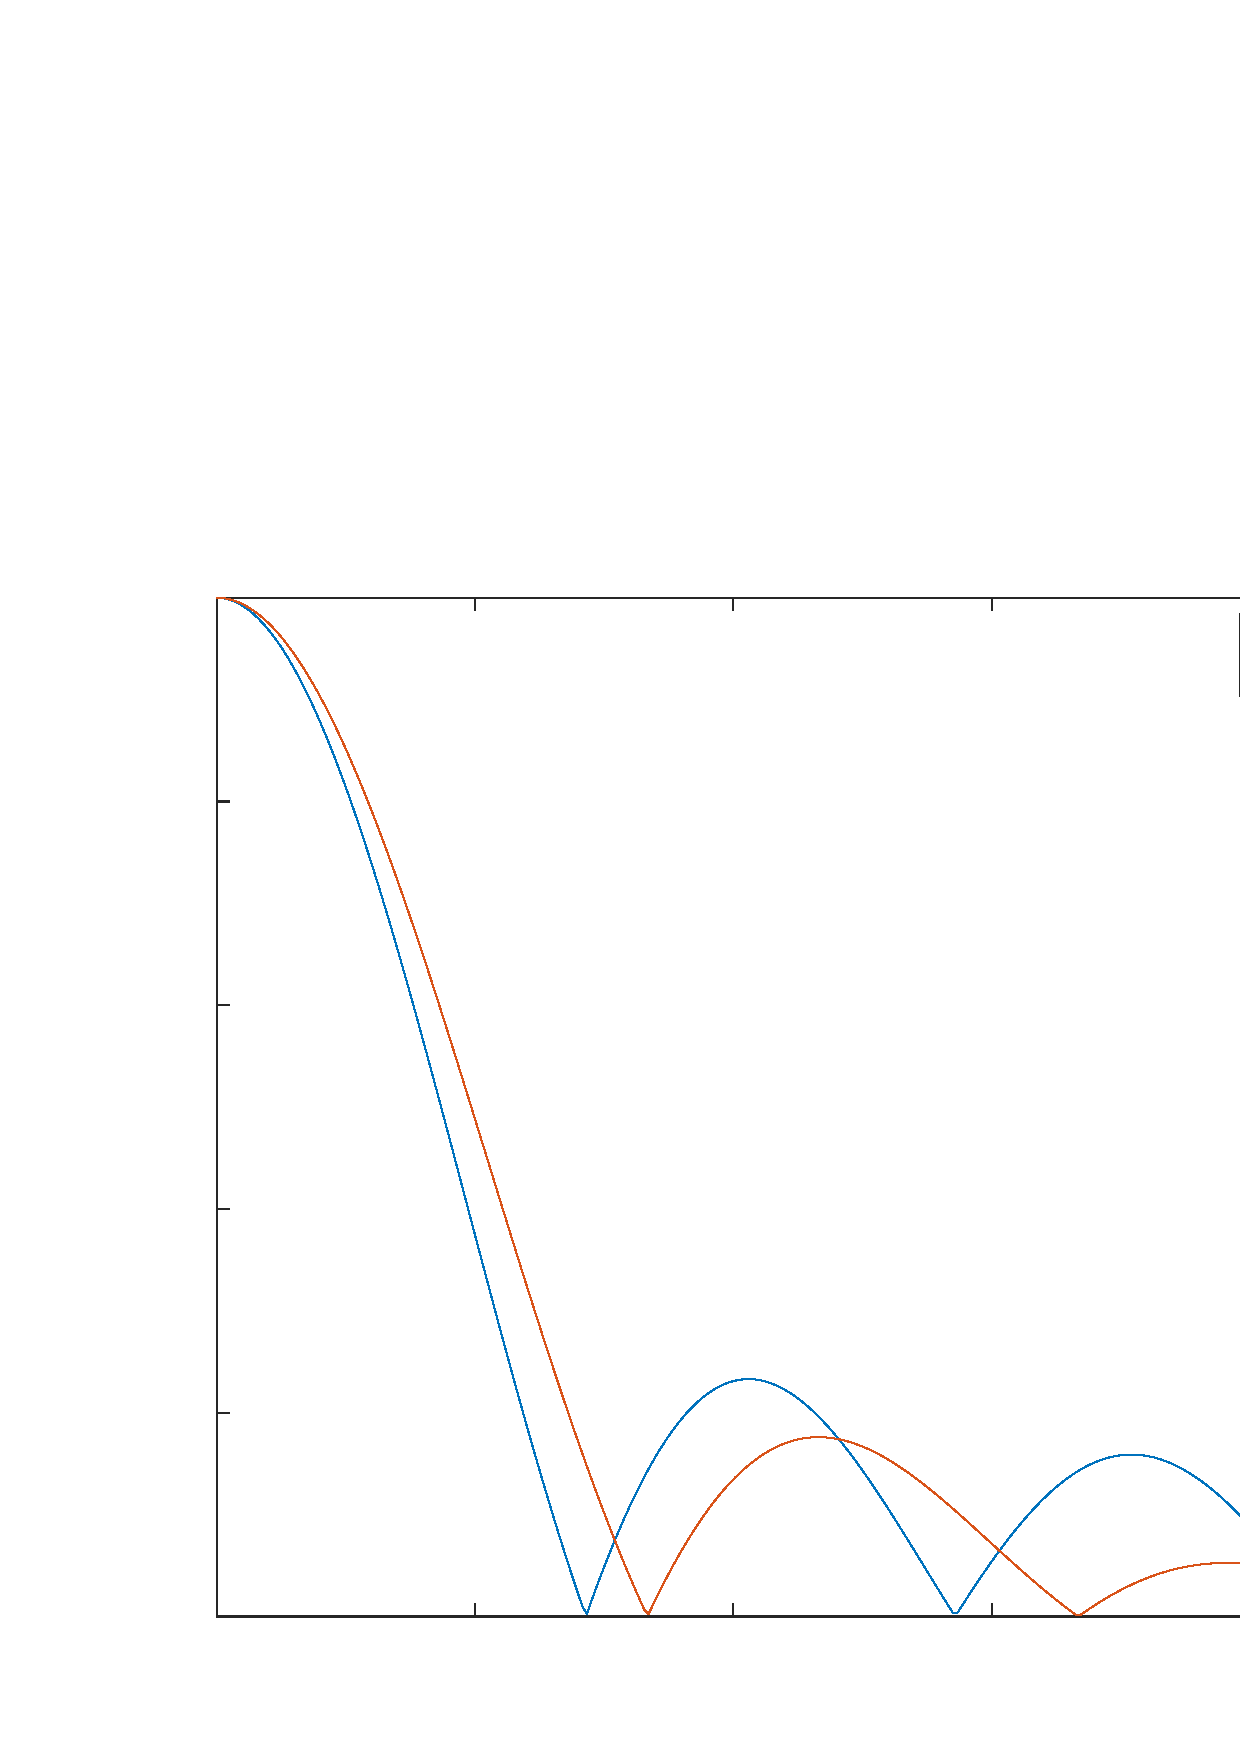
\includegraphics[scale=1]{octaves/typeI-inc}
\end{picture}%
\begin{picture}(800,600)(0,0)
\fontsize{13}{0}\selectfont\put(104,55.5788){\makebox(0,0)[t]{\textcolor[rgb]{0.15,0.15,0.15}{{0}}}}
\fontsize{13}{0}\selectfont\put(228,55.5788){\makebox(0,0)[t]{\textcolor[rgb]{0.15,0.15,0.15}{{0.2}}}}
\fontsize{13}{0}\selectfont\put(352,55.5788){\makebox(0,0)[t]{\textcolor[rgb]{0.15,0.15,0.15}{{0.4}}}}
\fontsize{13}{0}\selectfont\put(476,55.5788){\makebox(0,0)[t]{\textcolor[rgb]{0.15,0.15,0.15}{{0.6}}}}
\fontsize{13}{0}\selectfont\put(600,55.5788){\makebox(0,0)[t]{\textcolor[rgb]{0.15,0.15,0.15}{{0.8}}}}
\fontsize{13}{0}\selectfont\put(724,55.5788){\makebox(0,0)[t]{\textcolor[rgb]{0.15,0.15,0.15}{{1}}}}
\fontsize{13}{0}\selectfont\put(97.0525,66){\makebox(0,0)[r]{\textcolor[rgb]{0.15,0.15,0.15}{{0}}}}
\fontsize{13}{0}\selectfont\put(97.0525,163.8){\makebox(0,0)[r]{\textcolor[rgb]{0.15,0.15,0.15}{{0.2}}}}
\fontsize{13}{0}\selectfont\put(97.0525,261.6){\makebox(0,0)[r]{\textcolor[rgb]{0.15,0.15,0.15}{{0.4}}}}
\fontsize{13}{0}\selectfont\put(97.0525,359.4){\makebox(0,0)[r]{\textcolor[rgb]{0.15,0.15,0.15}{{0.6}}}}
\fontsize{13}{0}\selectfont\put(97.0525,457.2){\makebox(0,0)[r]{\textcolor[rgb]{0.15,0.15,0.15}{{0.8}}}}
\fontsize{13}{0}\selectfont\put(97.0525,555){\makebox(0,0)[r]{\textcolor[rgb]{0.15,0.15,0.15}{{1}}}}
\fontsize{15}{0}\selectfont\put(414,565){\makebox(0,0)[b]{\textcolor[rgb]{0,0,0}{{Magnitude response}}}}
\fontsize{12}{0}\selectfont\put(623.005,536.505){\makebox(0,0)[l]{\textcolor[rgb]{0,0,0}{{Moving average}}}}
\fontsize{12}{0}\selectfont\put(623.005,519.007){\makebox(0,0)[l]{\textcolor[rgb]{0,0,0}{{Type 1}}}}
\end{picture}

}\caption{Plot of the magnitude response of Type 1 FIR filter $H_7(z)$ in example and a $7$-point moving average filter, as described in~\ref{eqn:mPointMovingAverageEquation}. The two filters are very similar in their amplitude response, although different in how they `bounce' in the frequency domain. The frequency response has been improved by halving the first and the last coefficients of the impulse response.}\label{oct:typeI}
\end{center}
\end{figure*}

In this case, the degree $N$ of the transfer function is an even number. Let, for instance, $N=8$: the transfer function $H(z)$ will have a general form of
\begin{align*}
    H(z) &= h[0]
        + h[1]z^{-1}
        + h[2]z^{-2}
        + h[3]z^{-3}
        + h[4]z^{-4}\\
        & + h[5]z^{-5}
        + h[6]z^{-6}
        + h[7]z^{-7}
        + h[8]z^{-8},
\end{align*}
and because of symmetry induced by an even amplitude response by hypothesis, the following holds,
\begin{align*}
    h[0] &= h[8];\\
    h[1] &= h[7];\\
    h[2] &= h[6];\\
    h[3] &= h[5];
\end{align*}
and $h[4]$ will be the only sample not involved in a symmetric pair, as it's the center of symmetry. Therefore, we can write
\begin{align*}
    H(z) &= h[0](z^{-1} + z^{-8})
        + h[1](z^{-1} + z^{-7})
        + h[2](z^{-2} + z^{-6})\\
        & + h[3](z^{-3} + z^{-5})
        + h[4]z^{-4}\\
         &= z^{-4}\left(h[0](z^{4} + z^{-4})
        + h[1](z^{3} + z^{-3})
        + h[2](z^{2} + z^{-2})\right.\\
        & \left.+ h[3](z + z^{-1})
        + h[4]\right).
\end{align*}

The corresponding frequency response will be
\begin{align*}
    H(e^{j\omega}) &= e^{-j 4\omega}\left(2h[0]\cos{(4\omega)} + 2h[1]\cos{(3\omega)}\right.\\
    & + \left. 2h[2]\cos{(2\omega)} + 2h[3]\cos{(\omega)} + h[4]\right),
\end{align*}
as
\[
    e^{-j\varphi\omega} + e^{j\varphi\omega} = 2\cos{(\varphi \omega)}.
\]

The quantity inside the parentheses is a real function of $\omega$, and can assume positive or negative values in the frequency range of $0 \leq |\omega| \leq \pi$.

The phase function is given by
\[
    \theta(\omega) = -4\omega + \beta
\]
with the choice of $N=8$. Value of $\beta$ can either be $0$ or $\pi$ as the amplitude function is an even function---hence, the phase function is a linear function in $\omega$. The corresponding group delay is
\[
    \tau(\omega) = -\frac{d\theta(\omega)}{d\omega} = +4
\]
Since $c=-\frac N 2$, a generic choice of $N = 2\kappa$ would lead to a phase function of 
\begin{equation}\label{eqn:linearPhaseTypeIPhaseFunction}
    \theta(\omega) = -\kappa\omega + \beta
\end{equation}
and a group delay of
\begin{equation}\label{eqn:linearPhaseTypeIGroupDelay}
    \tau(\omega) = -\frac{d\theta(\omega)}{d\omega} = +\kappa.
\end{equation}

The group delay of a linear phase transfer function with an even amplitude response and an odd length--degree $N$ is a constant delay of value $\kappa = \frac {N}{2}$, with $\kappa$ being an \emph{integer} value. (Remember that, in order to obtain an odd length $N+1$, an even $N$ must be chosen.) As the amplitude response is an even function, either $\beta=0$ or $\beta=\pi$.

Generally speaking, for \textbf{Type 1} FIR filters with $\kappa = \frac N 2$ the frequency response has the form
\begin{equation}\label{eqn:linearPhaseTypeIResponse}
    H(e^{j\omega}) = e^{-j\kappa\omega}\breve{H}(\omega),
\end{equation}
with an (even) amplitude response of the form
\begin{equation}\label{eqn:linearPhaseTypeIAmplitudeResponse}
    \breve{H}(\omega) = h[\kappa] + 2\sum_{n=1}^\kappa h[\kappa - n]\cos{(\omega n)}.
\end{equation}

An example of a Type 1 FIR filter can be the following, of length $7$,
\[
    H_7(z) = \frac 1 6 \left[\frac 1 2 + z^{-1} + z^{-2} + z^{-3} + z^{-4} + z^{-5} + \frac 1 2z^{-6}\right],
\]
which could be seen as a slightly modified version of a $7$-point moving average filter, as in \ref{eqn:mPointMovingAverageEquation}. (To point out the differences, two samples of the impulse response are halved, and that is the discrepancy between the classic $M$-point moving average filter and this Type 1 FIR filter.) Since the above impulse response is symmetric and its length is odd, then it will possess the linear phase property of a Type 1 filter. Plots of the magnitude response of both $H_7(z)$ and a $7$-point moving average filter are shown in Figure~\ref{oct:typeI}. The impulse response has been improved by simply halving the first and the last coefficients---verily, the above Type 1 FIR filter is equivalent to the cascade of two moving average filters, the first of length $2$ and the second of length $6$:
\[
    H_7(z) = \underbrace{\frac 1 2\left(1 + z^{-1}\right)}_{M=2}\cdot\underbrace{\frac 1 6 \left(1 + z^{-1} + z^{-2} + z^{-3} + z^{-4} + z^{-5}\right)}_{M=6},
\]
and for this reason $H_7(z)$ has a double zero at $z=-1$, which means $\omega = \pi$ in the unit circle---this allows to concretely push to $0$ the magnitude response at the very high frequencies, and ultimately improve the frequency response.


\section{Type 2: Symmetric impulse response with even length and odd $N$}

For transfer functions of \textbf{Type 2}, the degree $N$ is an \textbf{odd} number in order for the length $N+1$ to be an even number. Let's assume---for simplicity---$N=7$; the transfer function will be of the form, generally, of
\begin{align*}
    H(z) &= h[0]
        + h[1]z^{-1}
        + h[2]z^{-2}
        + h[3]z^{-3}
        + h[4]z^{-4}\\
        & + h[5]z^{-5}
        + h[6]z^{-6}
        + h[7]z^{-7},
\end{align*}
and for symmetry of the impulse response coefficients one can get the following
\begin{align*}
    H(z) &= h[0](1 + z^{-7})
        + h[1](z^{-1} + z^{-6})\\
        & + h[2](z^{-2} + z^{-5})
        + h[3](z^{-3} + z^{-4})\\
         &= z^{-\frac 7 2}\left(h[0](z^{\frac 7 2} + z^{-\frac 7 2})
        + h[1](z^{\frac 5 2} + z^{-\frac 5 2})\right.\\
        & \left.+ h[2](z^{\frac 3 2} + z^{-\frac 32})
        + h[3](z^{\frac 1 2} + z^{-\frac 1 2})\right).
\end{align*}

The corresponding frequency response will be
\begin{align*}
    H(e^{j\omega}) &= e^{-j\frac 7 2 \omega} \left(2h[0]\cos{(\frac 7 2 \omega)} + 2h[1] \cos{(\frac 5 2 \omega)}\right.\\
    &\left. + 2h[2]\cos{(\frac 3 2 \omega)} + 2h[3] \cos{(\frac 1 2 \omega)} \right).
\end{align*}

As before, the quantity inside the parentheses is a real function in $\omega$, and can assume positive or negative values in the frequency range $0 \leq |\omega| \leq \pi$. Similarly, the phase function is given by
\[
    \theta(\omega) = -\frac 7 2 \omega + \beta,
\]
with $\beta$ either equal to $0$ or equal to $\pi$, since the amplitude response is an even function. The above formula proves that the phase function is a \emph{linear} function of $\omega$. The corresponding \textbf{group delay} is, again, a constant,
\[
    \tau(\omega) = +\frac 7 2,
\]
a constant delay of $\frac 7 2$ samples.

Since $c=-\frac N 2$, a generic choice of $N = 2\kappa$, that is $\kappa = \frac N 2$ would lead to a phase function of 
\begin{equation}\label{eqn:linearPhaseTypeIIPhaseFunction}
    \theta(\omega) = -\kappa\omega + \beta
\end{equation}
and a group delay of
\begin{equation}\label{eqn:linearPhaseTypeIIGroupDelay}
    \tau(\omega) = -\frac{d\theta(\omega)}{d\omega} = +\kappa,
\end{equation}
but this time $N$ is an odd number, and thus $\kappa$ should not be an integer number. The constant delay induced by the group delay would be the delay induced by a fractional number of samples. As the amplitude response is an even function, either $\beta=0$ or $\beta=\pi$.

In general, for \textbf{Type 2} FIR filters with $\kappa = \frac N 2$ (a fractional quantity) the frequency response has the form
\begin{equation}\label{eqn:linearPhaseTypeIIResponse}
    H(e^{j\omega}) = e^{-j\kappa\omega}\breve{H}(\omega),
\end{equation}
with an (even) amplitude response of the form
\begin{equation}\label{eqn:linearPhaseTypeIIAmplitudeResponse}
    \breve{H}(\omega) = 2\sum_{n=1}^{\frac{N+1}{2}} h[\frac{N+1}{2} - n]\cos{(\omega (n - \frac 1 2))}.
\end{equation}

Notice how, this time, the sum should be computed on $\frac {N+1}{2}$ terms instead of $\kappa = \frac N 2$ terms, as the term $h[\kappa]$ that was present in~\ref{eqn:linearPhaseTypeIAmplitudeResponse} ouside of the summation now is included in the summation for the above amplitude response formula. An even length (or, equivalently, an odd $N$) means that for Type 2 a ``central'' coefficient in the impulse response is missing, therefore the center of the impulse response will be located at $\kappa = \frac N 2$, resulting in a fractional value.


\section{Type 3: Anti-symmetric impulse response with odd length and even $N$}
The third type---the \textbf{Type 3} FIR filter---arises from an \textbf{odd} amplitude response (thus, will possess an anti-symmetric impulse response) and from an \textbf{odd} length (or, equivalently, from the choice of an even $N$). Since $N$ is an even number and for the anti-symmetry this type is subject to, the following always holds,
\begin{equation}\label{eqn:linearPhaseTypeIIIProperty}
    h[\frac N 2] = 0,
\end{equation}
as the impulse response coefficient located in the middle of the response must be equal to $0$ in order to satisfy the anti-symmetry requirement induced by an odd amplitude response.

Similarly to the previous two cases, let's assume---for simplicity---that $N=8$. Applying the anti-symmetry condition one gets
\begin{align*}
    H(z) &= z^{-4}\left(h[0](z^{4} - z^{-4})
         + h[1](z^{3} - z^{-3})\right.\\
         & \left.+ h[2](z^{2} - z^{-2})
         + h[3](z - z^{-1})\right).
\end{align*}
which is very similar to what occurred with Type 1, except that $h[4] = h[\frac 8 2] = 0$ and some minus signs due to the anti-symmetry. The corresponding frequency response is given by the following
\begin{align*}
    H(e^{j\omega}) &= e^{-j 4\omega}e^{j\frac \pi 2}\left(2h[0]\sin{(4\omega)} + 2h[1]\sin{(3\omega)}\right.\\
    & + \left. 2h[2]\sin{(2\omega)} + 2h[3]\sin{(\omega)}\right),
\end{align*}
as
\[
    e^{+j\varphi\omega} - e^{-j\varphi\omega} = 2j\sin{(\varphi \omega)}.
\]
A factor $e^{j\frac \pi 2}$ has been introduced, due to the Euler's formula when getting the sine function. (By way of clarification, $j = e^{j \frac \pi 2}$.)

The linear phase response is
\[
    \theta(\omega) = -4\omega + \frac \pi 2 + \beta,
\]
and, this time, $\beta$ could either be $\frac \pi 2$ or $-\frac \pi 2$, as the amplitude response is an odd function. The group delay is
\[
    \tau(\omega) = +4,
\]
and just like the previous cases it is a constant group delay. (More similarly to the Type 1, the group delay is an \emph{integer} constant delay.)

Since $c=-\frac N 2$, as always, a generic choice of $N = 2\kappa$ would lead to a phase function of 
\begin{equation}\label{eqn:linearPhaseTypeIIIPhaseFunction}
    \theta(\omega) = -\kappa\omega + \frac \pi 2 + \beta
\end{equation}
and a group delay of
\begin{equation}\label{eqn:linearPhaseTypeIIIGroupDelay}
    \tau(\omega) = -\frac{d\theta(\omega)}{d\omega} = +\kappa.
\end{equation}

The group delay of a linear phase transfer function with an even amplitude response and an odd length--degree $N$ is a constant delay of value $\kappa = \frac {N}{2}$, with $\kappa$ being an \emph{integer} value. As the amplitude response is an odd function, either $\beta=\frac \pi 2$ or $\beta=-\frac \pi 2$.

Generally speaking, for \textbf{Type 3} FIR filters with $\kappa = \frac N 2$ integer, the frequency response has the form
\begin{equation}\label{eqn:linearPhaseTypeIIIResponse}
    H(e^{j\omega}) = e^{-j\kappa\omega}\breve{H}(\omega),
\end{equation}
with an (odd) amplitude response of the form
\begin{equation}\label{eqn:linearPhaseTypeIIIAmplitudeResponse}
    \breve{H}(\omega) = 2\sum_{n=1}^\kappa h[\kappa - n]\sin{(\omega n)},
\end{equation}
and $h[\kappa] = 0$.

Very similar to the Type 1 amplitude response, still, the only difference is the presence of a sine function in place of a cosine function, which was caused by the anti-symmetry requirement (Type 3 filters are subject to an anti-symmetry property in place of a symmetry property).


\begin{figure*}[ht]
\begin{center}
    \begin{tikzpicture}
        \draw[-stealth] (-.5,0) -- (3,0) node[anchor=north west] {$n$};
        \draw[-stealth] (0,-.5) -- (0,1.6) node[anchor=south west] {$h_1[n]$};
        \draw[-{Circle[open]}] (0.3*0,0) -- (0.3*0,1);
        \draw[-{Circle[open]}] (0.3*1,0) -- (0.3*1,.6);
        \draw[-{Circle[open]}] (0.3*2,0) -- (0.3*2,-.4);
        \draw[-{Circle[open]}] (0.3*3,0) -- (0.3*3,.78);
        \draw[-{Circle[open]}] (0.3*4,0) -- (0.3*4,.4);
        \draw[-{Circle[open]}] (0.3*5,0) -- (0.3*5,.78);
        \draw[-{Circle[open]}] (0.3*6,0) -- (0.3*6,-.4);
        \draw[-{Circle[open]}] (0.3*7,0) -- (0.3*7,.6);
        \draw[-{Circle[open]}] (0.3*8,0) -- (0.3*8,1);
        \node at (0.3*0 - .1, -.2) {$0$};
        \node at (0.3*1, -.2) {$1$};
        \node at (0.3*2, +.2) {$2$};
        \node at (0.3*3, -.2) {$3$};
        \node at (0.3*4+.08, -.2) {$4$};
        \node at (0.3*5, -.2) {$5$};
        \node at (0.3*6, +.2) {$6$};
        \node at (0.3*7, -.2) {$7$};
        \node at (0.3*8, -.2) {$8$};
        \draw[dashed, thin] (0.3*4, -1.2) -- (0.3*4, 1.6);
        \node at (0.3*4 + .8, 1.4) {\tiny Center of symmetry};
    \end{tikzpicture}
    \begin{tikzpicture}
        \draw[-stealth] (-.5,0) -- (3,0) node[anchor=north west] {$n$};
        \draw[-stealth] (0,-.5) -- (0,1.6) node[anchor=south west] {$h_2[n]$};
        \draw[-{Circle[open]}] (0.3*0,0) -- (0.3*0,1);
        \draw[-{Circle[open]}] (0.3*1,0) -- (0.3*1,-.66);
        \draw[-{Circle[open]}] (0.3*2,0) -- (0.3*2,+.32);
        \draw[-{Circle[open]}] (0.3*3,0) -- (0.3*3,1.11);
        \draw[-{Circle[open]}] (0.3*4,0) -- (0.3*4,1.11);
        \draw[-{Circle[open]}] (0.3*5,0) -- (0.3*5,+.32);
        \draw[-{Circle[open]}] (0.3*6,0) -- (0.3*6,-.66);
        \draw[-{Circle[open]}] (0.3*7,0) -- (0.3*7,1);
        \node at (0.3*0 - .1, -.2) {$0$};
        \node at (0.3*1, +.2) {$1$};
        \node at (0.3*2, -.2) {$2$};
        \node at (0.3*3, -.2) {$3$};
        \node at (0.3*4, -.2) {$4$};
        \node at (0.3*5, -.2) {$5$};
        \node at (0.3*6, +.2) {$6$};
        \node at (0.3*7, -.2) {$7$};
        \draw[dashed, thin] (0.3*3.5, -1.2) -- (0.3*3.5, 1.6);
        \node at (0.3*3.5 + .8, 1.4) {\tiny Center of symmetry};
    \end{tikzpicture}
    \begin{tikzpicture}
        \draw[-stealth] (-.5,0) -- (3,0) node[anchor=north west] {$n$};
        \draw[-stealth] (0,-.5) -- (0,1.6) node[anchor=south west] {$h_3[n]$};
        \draw[-{Circle[open]}] (0.3*0,0) -- (0.3*0,1.3);
        \draw[-{Circle[open]}] (0.3*1,0) -- (0.3*1,.6);
        \draw[-{Circle[open]}] (0.3*2,0) -- (0.3*2,+.27);
        \draw[-{Circle[open]}] (0.3*3,0) -- (0.3*3,-.48);
        \node[draw, circle, inner sep=1.1pt, minimum size=0pt] at (0.3*4,0) {};
        \draw[-{Circle[open]}] (0.3*5,0) -- (0.3*5,.48);
        \draw[-{Circle[open]}] (0.3*6,0) -- (0.3*6,-.27);
        \draw[-{Circle[open]}] (0.3*7,0) -- (0.3*7,-.6);
        \draw[-{Circle[open]}] (0.3*8,0) -- (0.3*8,-1.3);
        \node at (0.3*0 - .1, -.2) {$0$};
        \node at (0.3*1, -.2) {$1$};
        \node at (0.3*2, -.2) {$2$};
        \node at (0.3*3, +.2) {$3$};
        \node at (0.3*4+.08, -.2) {$4$};
        \node at (0.3*5, -.2) {$5$};
        \node at (0.3*6, +.2) {$6$};
        \node at (0.3*7, +.2) {$7$};
        \node at (0.3*8, +.2) {$8$};
        \draw[dashed, thin] (0.3*4, -1.2) -- (0.3*4, 1.6);
        \node at (0.3*4 + .8, 1.4) {\tiny Center of symmetry};
    \end{tikzpicture}
    \begin{tikzpicture}
        \draw[-stealth] (-.5,0) -- (3,0) node[anchor=north west] {$n$};
        \draw[-stealth] (0,-.5) -- (0,1.6) node[anchor=south west] {$h_4[n]$};
        \draw[-{Circle[open]}] (0.3*0,0) -- (0.3*0,-.3);
        \draw[-{Circle[open]}] (0.3*1,0) -- (0.3*1,.7);
        \draw[-{Circle[open]}] (0.3*2,0) -- (0.3*2,-.4);
        \draw[-{Circle[open]}] (0.3*3,0) -- (0.3*3,-1);
        \draw[-{Circle[open]}] (0.3*4,0) -- (0.3*4,1);
        \draw[-{Circle[open]}] (0.3*5,0) -- (0.3*5,.4);
        \draw[-{Circle[open]}] (0.3*6,0) -- (0.3*6,-.7);
        \draw[-{Circle[open]}] (0.3*7,0) -- (0.3*7,.3);
        \node at (0.3*0 - .1, +.2) {$0$};
        \node at (0.3*1, -.2) {$1$};
        \node at (0.3*2, +.2) {$2$};
        \node at (0.3*3, +.2) {$3$};
        \node at (0.3*4, -.2) {$4$};
        \node at (0.3*5, -.2) {$5$};
        \node at (0.3*6, +.2) {$6$};
        \node at (0.3*7, -.2) {$7$};
        \draw[dashed, thin] (0.3*3.5, -1.2) -- (0.3*3.5, 1.6);
        \node at (0.3*3.5 + .8, 1.4) {\tiny Center of symmetry};
    \end{tikzpicture}\\
\end{center}\caption{Stem plots of example impulse responses of linear phase FIR filters, of types from $1$ to $4$. The first two types possess symmetric properties, while the last two show anti-symmetric properties---with the coefficient at the center of symmetry of Type 3 being equal to $0$. Type 2 and Type 4 have odd $N$ value, and thus exhibit a center of symmetry of fractional value.}\label{tikz:linearPhaseAllTypesImpulseResponses}
\end{figure*}

\section{Type 4: Anti-symmetric impulse response with even length and odd $N$}
In \textbf{Type 4}, the amplitude response is an odd function, and the degree $N$ is odd to obtain an even length of $N+1$. Let's assume $N=7$. The symmetry condition yields
\begin{align*}
    H(z) &= z^{-\frac 7 2}\left(h[0](z^{\frac 7 2} - z^{-\frac 7 2})
         + h[1](z^{\frac 5 2} - z^{-\frac 5 2})\right.\\
         & \left.+ h[2](z^{\frac 3 2} - z^{-\frac 32})
         + h[3](z^{\frac 1 2} - z^{-\frac 1 2})\right),
\end{align*}
analogously to Type 2 filters, but with some minus signs induced by the anti-symmetry property. Again, this will lead to sine functions in the frequency response,
\begin{align*}
    H(e^{j\omega}) &= e^{-j\frac 7 2 \omega} e^{j\frac \pi 2} \left(2h[0]\sin{(\frac 7 2 \omega)} + 2h[1] \sin{(\frac 5 2 \omega)}\right.\\
    &\left. + 2h[2]\sin{(\frac 3 2 \omega)} + 2h[3] \sin{(\frac 1 2 \omega)} \right).
\end{align*}
A factor $e^{j\frac \pi 2}$ has been introduced, again, for the same reasons as in Type 3 proceedings.

In this case, the phase response is
\[
    \theta(\omega) = - \frac 7 2 \omega + \frac \pi 2 + \beta,
\]
with either $\beta=\frac \pi 2$ or $\beta = - \frac \pi 2$. The group delay is constant and of a fractional value,
\[
    \tau(\omega) = \frac 7 2.
\]

Since $c=-\frac N 2$, a generic choice of $N = 2\kappa$, that is $\kappa = \frac N 2$ (in this case, a fractional value) would lead to a phase function of
\begin{equation}\label{eqn:linearPhaseTypeIVPhaseFunction}
    \theta(\omega) = -\kappa\omega + \frac \pi 2 + \beta
\end{equation}
and a group delay of
\begin{equation}\label{eqn:linearPhaseTypeIVGroupDelay}
    \tau(\omega) = -\frac{d\theta(\omega)}{d\omega} = +\kappa,
\end{equation}
but this time $N$ is an odd number, and thus $\kappa$ is not an integer number. The constant delay induced by the group delay would be the delay induced by a fractional number of samples. As the amplitude response is an odd function, either $\beta=\frac \pi 2$ or $\beta=- \frac \pi 2$.

In the general case, for \textbf{Type 4} FIR filters with $\kappa = \frac N 2$ (a fractional quantity) the frequency response has the form
\begin{equation}\label{eqn:linearPhaseTypeIVResponse}
    H(e^{j\omega}) = e^{-j\kappa\omega}\breve{H}(\omega),
\end{equation}
with an (odd) amplitude response of the form
\begin{equation}\label{eqn:linearPhaseTypeIVAmplitudeResponse}
    \breve{H}(\omega) = 2\sum_{n=1}^{\frac{N+1}{2}} h[\frac{N+1}{2} - n]\sin{(\omega (n - \frac 1 2))}.
\end{equation}


\section{General form of the frequency response}
In all four types of linear phase FIR filters, the \textbf{frequency response} has a general form, that is
\begin{equation}\label{eqn:linearPhaseGeneralResponse}
    H(e^{j\omega}) = e^{-j\frac N 2 \omega}e^{j\beta}\breve{H}(\omega).
\end{equation}

The amplitude response, in general, can become negative over certain frequency ranges; typically, it will become negative \emph{in the stopband}. In particular, the \textbf{magnitude} and \textbf{phase response} of linear phase FIR filters are given by the following two formulas,
\begin{equation}\label{eqn:linearPhaseGeneralMagnitudeResponse}
    \left|H(e^{j\omega})\right| = \left|\breve{H}(\omega)\right|,
\end{equation}
and
\begin{equation}\label{eqn:linearPhaseGeneralPhaseResponse}
    \theta(\omega) = 
    \left\{
        \begin{array}{ll}
            -\frac N 2 \omega + \beta, & \breve{H}(\omega) \leq 0\\
            -\frac N 2 \omega + \beta - \pi, & \breve{H}(\omega) < 0
        \end{array}
    \right..
\end{equation}
In each and every case, the \textbf{group delay}, with $\kappa = \frac N 2$, will be
\begin{equation}\label{eqn:linearPhaseGeneralGroupDelay}
    \tau(\omega) = +\kappa = +\frac N 2,
\end{equation}
will always be a \emph{constant delay}, either of a fractional quantity or an integer quantity depending whether $N$ is even or odd. Note that, even though the group delay is a constant, the output waveform \textbf{is not} a replica of the input wavform (indeed, the amplitude response might vary the signal over frequency, as $\left|\breve{H}(\omega)\right|$ is not, in general, a constant).

To conclude the perspective over linear phase FIR filters Types, any FIR filter with a \textbf{real frequency response} of $\omega$ is said to be a \textbf{zero phase filter}---such a filter must possess a noncausal impulse response.

\subsection{Location of zeros in Linear-phase FIR transfer functions}
Let $h[n]$ be a \emph{symmetric} impulse response of a FIR filter with length $N+1$, that is an impulse response that satisfies property $h[n] \equiv h[N-n]$. Due to symmetry, its transfer function can be rewritten as
\[
    H(z) = \sum_{n=0}^N h[n]z^{-n} = \sum_{n=0}^N h[N-n]z^{-n}.
\]

By the change of variable $m = N - n$, one can soon re\"express the above as
\[
    \sum_{n=0}^N h[N-n]z^{-n} = \sum_{m=0}^N h[m]z^{-N+m} = z^{-N}\sum_{m=0}^N h[m]z^{+m},
\]
which clearly leads to
\[
    H(z) = \sum_{n=0}^N h[N-n]z^{-n} = z^{-N}\underbrace{\sum_{m=0}^N h[m]z^{-m}}_{H(z^{-1})} = z^{-N}H(z^{-1}),
\]
and definitely
\[
    H(z) =  z^{-N}H(z^{-1}).
\]

As one might recall, any polynomial with \emph{real coefficients} satisfying Equation~\ref{eqn:mirrorImagePolynomial} is called a \textbf{mirror-image polynomial}---that is the same relationship as above. Thus, any $H(z)$ satisfying the above will also be a \emph{mirror-image polynomial} transfer function.

To name an example, let
\[
    H(z) = a_0 + a_1z^{-1} + a_2z^{-2} + a_2z^{-3} + a_1z^{-4} + a_0z^{-5}
\]
be a polynomial in $z$. One has
\begin{align*}
    z^{-5}H(z^{-1}) &= z^{-5}(a_0 + a_1z^{1} + a_2z^{2} + a_2z^{3} + a_1z^{4} + a_0z^{5}) \\
                    &= a_0z^{-5} + a_1z^{-4} + a_2z^{-3} + a_2z^{-2} + a_1z^{-1} + a_0 \\
                    &= a_0 + a_1z^{-1} + a_2z^{-2} + a_2z^{-3} + a_1z^{-4} + a_0z^{-5} \\
                    &= H(z).
\end{align*}

Note that this only works because $h[n] \equiv h[N-n]$, due to the symmetry property with which the impulse response $h$ was supposed to comply from the beginning. What's the case of an anti-symmetric impulse response then?

Let's try with an anti-symmetric impulse response $h[n]$ of, again, a FIR filter, which has to comply with $h[n] \equiv -h[N-n]$. With the same logic as before, let's rewrite the transfer function into something different
\[
    H(z) = \sum_{n=0}^N h[n]z^{-n} = -\sum_{n=0}^N h[N-n]z^{-n},
\]
and going through the change of variable $m = N - n$ same as before, one is able to re\"express the above as
\[
    -\sum_{n=0}^N h[N-n]z^{-n} = -\sum_{m=0}^N h[m] z^{-N+m} = -z^{-N}H(z^{-1});
\]
this inevitably leads to
\[
    H(z) = -z^{-N}H(z^{-1}).
\]

Just like the previous case, this time we can refer to Equation~\ref{eqn:antimirrorImagePolynomial}, and we can say that any transfer function $H(z)$ of \emph{real coefficients} that abides to the above resulting equation will be an \textbf{antimirror-image polynomial} transfer function. 

Similarly, we can craft an example that can speak for itself---let $H(z)$ be an antimirror-image polynomial
\[
    H(z) = a_0 + a_1z^{-1} + a_2z^{-2} - a_2z^{-3} - a_1z^{-4} - a_0z^{-5}.
\]

Hence,
\begin{align*}
    -z^{-5}H(z^{-1}) &= -z^{-5}(a_0 + a_1z^{1} + a_2z^{2} - a_2z^{3} - a_1z^{4} - a_0z^{5})\\
                     &= a_0z^{-5} + a_1z^{-4} + a_2z^{-3} - a_2z^{-2} - a_1z^{-1} - a_0\\
                     &= a_0 + a_1z^{-1} + a_2z^{-2} - a_2z^{-3} - a_1z^{-4} - a_0z^{-5}\\
                     &= H(z).
\end{align*}

These two scenarios of symmetric and anti-symmetric transfer functions---the mirror-image polynomial and the antimirror-image polynomial---are not just a mere showoff: instead, the two concepts lay the foundations for a simple way to find the zeros of a FIR filter that abides to some symmetry or anti-symmetry rule. Indeed, by looking at the (anti)mirror image of a transfer function of that kind,
\[
    H(z) = \pm z^{-N}H(z^{-1})
\]
one can easily infer that if $z=\xi_0$ is a zero of $H(z)$, then $z=\frac 1 {\xi_0}$ must be a zero as well. (To explain that, simply recall the results highlighted in Section~\ref{sec:allpassTransferFunctions}, which explains how mirror-image polynomials of real-coefficient transfer functions possess pairs of zeros located in the `mirror' position, that is the reciprocal of the value of the zero.)

Additionally, if the impulse response is totally real-valued, then the zeros of $H(z)$ will occur in \emph{complex--conjugate pairs}; but this means that for any zero $z=\xi_0$ there will be a conjugate associated twin at $z=\xi^*_0$. This leads to the following, crucial result for linear-phase FIR filters: any complex zero that is not in the unit circle will be associated to other $3$ zeros, forming \textbf{a set of $4$ zeros} given by the following expressions
\begin{eqnarray}\label{eqn:linearPhaseGeneralZeroLocationsSet}
    z_{1,2} = r e^{\pm j\varphi}, \\
    z_{3,4} = \frac 1 r e^{\pm j\varphi}.
\end{eqnarray}

If a zero lies on the unit circle, it appears \textbf{as a pair only}
\begin{equation}\label{eqn:linearPhaseGeneralZeroLocationsPair}
    z_{1,2} = e^{\pm j\varphi},
\end{equation}
as the reciprocal has the same `mirror' location of the mirrored zero, since $r \equiv \frac 1 r$. In this case, the (anti)mirror-image pair overlap, leaving the complex--conjugate pair alone.

If a zero is real, then its reciprocal appears at the mirror location, and the zeros will appear \textbf{as a pair}. In this case, the complex--conjugate pair will overlap, and there will only be the (anti)mirror-image pair left,
\begin{eqnarray}\label{eqn:linearPhaseGeneralZeroLocationsPairReal}
    z_1 = \alpha, \\
    z_2 = \frac 1 \alpha.
\end{eqnarray}

Finally, all $4$ zeros will appear \textbf{the same} if $z=\pm1$; that's because both the complex--conjugate pair and the (anti)mirror-image pair will overlap.

After looking at how the sets of zeros are built---namely, there must be both a complex--conjugate pair and an (anti)mirror-image pair, which could possibly overlap---we will now discover that some \emph{constraints} on zero locations exist, depending on the types of linear-phase transfer functions. 

The following list explains such constraints and properties, and also contains example illustrations for each type.

\begin{description}
    \item[Type 2] A Type 2 FIR filter will have a zero at $z=-1$. In point of fact, since it satisfies
        \[
            H(z) = z^{-N}H(z^{-1}), N \mbox{ odd }
        \]
        then
        \[
            H(-1) = (-1)^{-N} H(-1) = -H(-1) \equiv 0,
        \]
        which proves the claim;
        \begin{center}
            \begin{tikzpicture}
                \draw[thick,-stealth] (-3.0,0) -- (3.0,0) node[anchor=north west] {$\Re z$};
                \draw[thick,-stealth] (0,-3.0) -- (0,3.0) node[anchor=south east] {$\Im z$};
                \draw (1pt, 2.0) -- (-1pt, 2.0) node[anchor=north east] {$1$};
                \node[draw, circle, thick, minimum size=4cm] at (0,0) {};
                \node[draw, zeroz, thick] at (-2, 0) {};
                \node[draw, zeroz, thick, red] at (.4, 1.6) {};
                \node[draw, zeroz, thick, red] at (.6, 2.5) {};
                \node[draw, zeroz, thick, red] at (.4, -1.6) {};
                \node[draw, zeroz, thick, red] at (.6, -2.5) {};
                \node[draw, zeroz, thick, green] at (1.8, 0) {};
                \node[draw, zeroz, thick, green] at (2.22, 0) {};
                \node[draw, zeroz, thick, blue] at (-.5, 1.9378) {};
                \node[draw, zeroz, thick, blue] at (-.5, -1.9378) {};
                \node[draw, zeroz, thick, purple] at (-1.7, .6) {};
                \node[draw, zeroz, thick, purple] at (-1.7, -.6) {};
                \node[draw, zeroz, thick, purple] at (-2.2, 0.766) {};
                \node[draw, zeroz, thick, purple] at (-2.2, -0.766) {};
            \end{tikzpicture}
        \end{center}
    \item[Type 4] Type 4 FIR filters will have a zero at $z=+1$. Indeed, it satisfies
        \[
            H(z) = -z^{-N}H(z^{-1}), N \mbox{ odd },
        \]
        which results in
        \[
            H(1) = -(1)^{-N} H(1) = -H(1) \equiv 0,
        \]
        forcing a zero at $z=+1$;
        \begin{center}
            \begin{tikzpicture}
                \draw[thick,-stealth] (-3.0,0) -- (3.0,0) node[anchor=north west] {$\Re z$};
                \draw[thick,-stealth] (0,-3.0) -- (0,3.0) node[anchor=south east] {$\Im z$};
                \draw (1pt, 2.0) -- (-1pt, 2.0) node[anchor=north east] {$1$};
                \node[draw, circle, thick, minimum size=4cm] at (0,0) {};
                \node[draw, zeroz, thick] at (+2, 0) {};
                \node[draw, zeroz, thick, red] at (.4, 1.6) {};
                \node[draw, zeroz, thick, red] at (.6, 2.5) {};
                \node[draw, zeroz, thick, red] at (.4, -1.6) {};
                \node[draw, zeroz, thick, red] at (.6, -2.5) {};
                \node[draw, zeroz, thick, green] at (1.8, 0) {};
                \node[draw, zeroz, thick, green] at (2.22, 0) {};
                \node[draw, zeroz, thick, blue] at (-.5, 1.9378) {};
                \node[draw, zeroz, thick, blue] at (-.5, -1.9378) {};
                \node[draw, zeroz, thick, purple] at (-1.7, .6) {};
                \node[draw, zeroz, thick, purple] at (-1.7, -.6) {};
                \node[draw, zeroz, thick, purple] at (-2.2, 0.766) {};
                \node[draw, zeroz, thick, purple] at (-2.2, -0.766) {};
            \end{tikzpicture}
        \end{center}
    \item[Type 3] Any Type 3 FIR filter will be forced to have at least two zeros: one at $z=+1$ and the other one at $z=-1$. Verily, they must abide to
        \[
            H(z) = -z^{-N}H(z^{-1}), N \mbox{ even },
        \]
        and for this reason both
        \[
            H(1) = -(1)^{-N}H(1) = -H(1) \equiv 0
        \]
        and
        \[
            H(-1) = -(-1)^{-N}H(-1) = -H(-1) \equiv 0
        \]
        are true, forcing the two zeros to exist;
        \begin{center}
            \begin{tikzpicture}
                \draw[thick,-stealth] (-3.0,0) -- (3.0,0) node[anchor=north west] {$\Re z$};
                \draw[thick,-stealth] (0,-3.0) -- (0,3.0) node[anchor=south east] {$\Im z$};
                \draw (1pt, 2.0) -- (-1pt, 2.0) node[anchor=north east] {$1$};
                \node[draw, circle, thick, minimum size=4cm] at (0,0) {};
                \node[draw, zeroz, thick] at (+2, 0) {};
                \node[draw, zeroz, thick] at (-2, 0) {};
                \node[draw, zeroz, thick, red] at (.4, 1.6) {};
                \node[draw, zeroz, thick, red] at (.6, 2.5) {};
                \node[draw, zeroz, thick, red] at (.4, -1.6) {};
                \node[draw, zeroz, thick, red] at (.6, -2.5) {};
                \node[draw, zeroz, thick, green] at (1.8, 0) {};
                \node[draw, zeroz, thick, green] at (2.22, 0) {};
                \node[draw, zeroz, thick, blue] at (-.5, 1.9378) {};
                \node[draw, zeroz, thick, blue] at (-.5, -1.9378) {};
                \node[draw, zeroz, thick, purple] at (-1.7, .6) {};
                \node[draw, zeroz, thick, purple] at (-1.7, -.6) {};
                \node[draw, zeroz, thick, purple] at (-2.2, 0.766) {};
                \node[draw, zeroz, thick, purple] at (-2.2, -0.766) {};
            \end{tikzpicture}
        \end{center}
    \item[Type 1] Type 1 FIR filters are not subject to any of the phenomena that occur for the other three types of FIR filters---indeed, they must follow
        \[
            H(z) = z^{-N}H(z^{-1}), N \mbox{ even },
        \]
        which leads to no forced zeros at all.
        \begin{center}
            \begin{tikzpicture}
                \draw[thick,-stealth] (-3.0,0) -- (3.0,0) node[anchor=north west] {$\Re z$};
                \draw[thick,-stealth] (0,-3.0) -- (0,3.0) node[anchor=south east] {$\Im z$};
                \draw (1pt, 2.0) -- (-1pt, 2.0) node[anchor=north east] {$1$};
                \node[draw, circle, thick, minimum size=4cm] at (0,0) {};
                \node[draw, zeroz, thick, red] at (.4, 1.6) {};
                \node[draw, zeroz, thick, red] at (.6, 2.5) {};
                \node[draw, zeroz, thick, red] at (.4, -1.6) {};
                \node[draw, zeroz, thick, red] at (.6, -2.5) {};
                \node[draw, zeroz, thick, green] at (1.8, 0) {};
                \node[draw, zeroz, thick, green] at (2.22, 0) {};
                \node[draw, zeroz, thick, blue] at (-.5, 1.9378) {};
                \node[draw, zeroz, thick, blue] at (-.5, -1.9378) {};
                \node[draw, zeroz, thick, purple] at (-1.7, .6) {};
                \node[draw, zeroz, thick, purple] at (-1.7, -.6) {};
                \node[draw, zeroz, thick, purple] at (-2.2, 0.766) {};
                \node[draw, zeroz, thick, purple] at (-2.2, -0.766) {};
            \end{tikzpicture}
        \end{center}
\end{description}

Of course, nothing prevents any of the above types to possess \textbf{additional} zeros at both $z=-1$ and $z=+1$: what the above results tell, instead, is that \emph{single} zeros exist at specified locations regardless of the polynomial feats. This means that
\begin{itemize}
    \item \emph{Type 1} filters will either have an even number of zeros or no zeros at $z=1$ and $z=-1$;
    \item \emph{Type 2} filters will either have an even number of zeros or no zeros at $z=1$, and an odd number of zeros at $z=-1$;
    \item \emph{Type 3} filters will have an odd number of zeros at both $z=1$ and $z=-1$;
    \item \emph{Type 4} filters will either have an even number of zeros or no zeros at $z=-1$, and an odd number of zeros at $z=1$.
\end{itemize}

We can then summarize the results into the following Table,
\begin{table}[ht]
\centering
\begin{tabular}{c|ll}
    \textbf{Filter type} & \textbf{Zeros at} $z=1$ & \textbf{Zeros at} $z=-1$ \\
    \hline
    1 & even or none & even or none\\
    2 & even or none & odd\\
    3 & odd & odd\\
    4 & odd & even or none
\end{tabular}
\caption{Number of zeros at $z=\pm 1$ for different types of linear-phase FIR filters.}\label{tab:linearPhaseGeneralZeroNumbers}
\end{table}
\bigskip

Some notable consequences derive from the above results---the mandatory zeros at $z = \pm 1$ introduce some possible shortcomings when it comes to filter design. Very much,
\begin{description}
    \item[Type 2] Design of \emph{highpass} and \emph{bandstop} filters is not possible, due to the zero at $\omega=\pi$;
    \item[Type 3] Design of \emph{lowpass}, \emph{highpass} or \emph{bandstop} filters is not possible, since there are two unavoidable zeros, one at $\omega = 0$ and the other one at $\omega = \pi$;
    \item[Type 4] Design of \emph{lowpass} and \emph{bandstop} filters is not possible, as the zero at $\omega = 0$ makes it impossible;
    \item[Type 1] Type 1 filters have no mandatory zeros, therefore \textbf{they freely allow any kind of design}.
\end{description}

\chapter{Simple Digital Filters}

Digital filters design involves composing a filter that is capable of satisfying some prescribed \emph{specifications}---later on, more advanced techniques to do so will be provided. For the moment, a battery of simple digital filters will be addressed, with reasonable selective frequency responses that are satisfactory in a number of convenient applications.

All simple digital filters hereby listed have integer-valued impulse responses coefficients. Moreover, since they are very simple filters, inexpensive hardware can be exploited for their practical realization.

\section{Lowpass FIR digital filters}

\textbf{Lowpass FIR digital filters} are the first category of simple digital filters we will encounter. The simplest of them is the $2$-point moving average filter, that is given by the following
\begin{equation}\label{eqn:twoPointMovingAverageFilterFIRLowpass}
    H_0(z) = \frac 1 2 \left(1 + z^{-1}\right) = \frac {z+1} {2z}.
\end{equation}

The above transfer function is symmetric and of even length (hence, $N$ is odd)---a Type 2 transfer function. For this reason, it will possess a zero in $\zeta=-1$ and additionally a pole in $\xi = 0$. A digital FIR filter of this kind will possess a zero at high frequencies $\omega = \pi$, while keeping the magnitude of any other point as close to the input value as this configurations makes possible---indeed, the \emph{pole vector} (the vector from the pole to the unit circle when going through $\omega$ frequencies) will have a constant module of $1$, as shown in the next graph.

\begin{center}
    \begin{tikzpicture}
        \draw[thick,-stealth] (-3.0,0) -- (3.0,0) node[anchor=north west] {$\Re z$};
        \draw[thick,-stealth] (0,-3.0) -- (0,3.0) node[anchor=south east] {$\Im z$};
        \draw (2.0, 1pt) -- (2.0, -1pt) node[anchor=north east] {$1$};
        \draw (-2.0, 1pt) -- (-2.0, -1pt) node[anchor=north east] {$-1$};
        \node[draw, circle, thick, minimum size=4cm] at (0,0) {};
        \node[draw, zeroz, thick](zero) at (-2, 0) {};
        \node[draw, polez, thick](pole) at (0, 0) {};
        \draw[-latex, green] (pole) -- (1.8421, 0.7788);
        \draw[-latex, blue] (zero) -- (1.8421, 0.7788);
        \draw[-latex, dashed, green] (pole) -- (1.3934, 1.4347);
        \draw[-latex, dashed, blue] (zero) -- (1.3934, 1.4347);
        \draw[-latex, dashed, green] (pole) -- (-1.6022, 1.1969);
        \draw[-latex, dashed, blue] (zero) -- (-1.6022, 1.1969);
        \draw[-latex, dashed, green] (pole) -- (-1.6022, 1.1969);
        \draw[-latex, dashed, blue] (zero) -- (-1.6022, 1.1969);
        \draw[-latex, dashed, green] (pole) -- (-0.4215, -1.9550);
        \draw[-latex, dashed, blue] (zero) -- (-0.4215, -1.9550);
        \node[] at (-2.35, .9)(hf) {$\omega = \pi$};
        \node[] at (2.35, .8)(lf) {$\omega = 0$};
        \draw[-stealth, dashed, thin] (hf) -- (zero);
        \draw[-stealth, dashed, thin] (lf) -- (2, 0);
    \end{tikzpicture}
\end{center}

The above figure shows that the pole vector (in green) will always have a constant module, whilst the zero vector (in blue) will be larger or smaller in magnitude depending on the current frequency $\omega$.
As the evaluation approaches high frequencies (very close to $\omega = \pi$), the zero gains importance and its contribution becomes relevant: the filter will act as a lowpass filter. 
Indeed, the zero vector starts with a magnitude of $2$---the radius of the unit circle---and goes down to a magnitude of $0$. 
The magnitude response $\left|H_0(\omega)\right|$ will be a monotonically decreasing function of $\omega$ in the interval $[0, \pi]$. 
The peak value is $\left|H_0(e^{j0})\right| = 1$ and the minimum is $\left|H_0(e^{j\pi})\right| = 0$: we have just built a very simple digital lowpass filter from the $M$-point moving average filter. 

The frequency response of the above filter will be
\begin{equation}\label{eqn:twoPointMovingAverageFilterFIRFrequencyResponse}
    H_0(e^{j\omega}) = e^{-j\frac \omega 2}\cos{(\frac \omega 2)}.
\end{equation}

Undoubtedly, by considering the magnitude response
\[
    \left|H_0(e^{j\omega})\right| = \cos{(\frac \omega 2)}
\]
it's rather straightforward to see that it is in fact a monotonically decreasing function in the interval $[0, \pi]$, as shown in the next plot.
\begin{center}
    \begin{tikzpicture}[
        ]
            \begin{axis}[
                at={(0,0)},
                xlabel = $\frac \omega \pi$,
                domain = 0:1,
                samples = 200,
                legend style = {
                at = {(0.5,1.02)},
                anchor = south},
                ]
                \addlegendentry{$\left|H_0(e^{j\omega})\right| = \cos{(\frac \omega 2)}$}
                        \addplot[mark = none, thick] gnuplot[raw gnuplot] {
                            set samples 200;
                            magnitude(x) = cos(0.5*x*pi);
                            plot[0:1] magnitude(x);
                    };
            \end{axis};
    \end{tikzpicture}
\end{center}

\begin{figure*}[ht]
    \begin{center}
        \begin{tikzpicture}[
            ]
                \begin{axis}[
                    at={(0,0)},
                    xlabel = $\frac \omega \pi$,
                    domain = 0:1,
                    samples = 200,
                    legend style = {
                    at = {(0.5,1.02)},
                    anchor = south},
                    ]
                    \addlegendentry{Single $\left|H_0(e^{j\omega})\right| = \cos{(\frac \omega 2)}$}
                            \addplot[mark = none, thick] gnuplot[raw gnuplot] {
                                set samples 200;
                                magnitude(x) = cos(0.5*x*pi);
                                plot[0:1] magnitude(x);
                        };
                \end{axis};
        \end{tikzpicture}
        \begin{tikzpicture}[
            ]
                \begin{axis}[
                    at={(0,0)},
                    xlabel = $\frac \omega \pi$,
                    domain = 0:1,
                    samples = 200,
                    legend style = {
                    at = {(0.5,1.02)},
                    anchor = south},
                    ]
                    \addlegendentry{Cascade of three $\left|H_0(e^{j\omega})\right| = \cos{(\frac \omega 2)}$}
                            \addplot[mark = none, thick] gnuplot[raw gnuplot] {
                                set samples 200;
                                magnitude(x) = cos(0.5*x*pi);
                                plot[0:1] magnitude(x)*magnitude(x)*magnitude(x);
                        };
                \end{axis};
        \end{tikzpicture}
    \end{center}\caption{Comparison between a single $2$-point moving average filter with magnitude frequency response $\left|H_0(e^{j\omega})\right| = \cos{(\frac \omega 2)}$ and a system composed of the cascode of three filters, all with the same magnitude frequency response $\left|H_0(e^{j\omega})\right|$. The system of three filters shows a better lowpass performance, at the expense of a smaller passband width.}\label{oct:simpleFiltersComparisonSingleThreeMPointMovingAverageFilters}
\end{figure*}

A peculiar frequency, which is of remarkable interest, is the frequency $\omega_c$ at which
\[
    \left|H_0(e^{j\omega_c})\right| = \frac{1}{\sqrt{2}} \left|H_0(e^{j0})\right|;
\]
at such frequency, the \textbf{gain} $\mathcal G (\omega_c)$, in decibel (dB), is given by
\begin{align*}
    \mathcal G(\omega_c) &= 20\log_{10}\left|H(e^{j\omega_c})\right|\\
                         &= 20\log_{10}\left|H(e^{j0})\right| - 20\log_{10}\sqrt{2}\\
                         &\simeq 3 \mbox{dB},
\end{align*}
as the gain $\mathcal G(0) = 20 \log_{10}\left|H(e^{j0})\right| = 0$. As a result, the gain $\mathcal G(\omega)$ at $\omega = \omega_c$ is approximately $3$ dB less than the gain at $\omega = 0$---the frequency $\omega_c$ is said to be the \textbf{3-dB Cutoff Frequency}.

The 3-dB cutoff frequency $\omega_c$ for any filter will be the frequency for which
\begin{equation}\label{eqn:cutoffFrequency}
    \left|H(e^{j\omega_c})\right| = \frac{1}{\sqrt{2}} \left|H(e^{j0})\right|,
\end{equation}
that corresponds to a gain loss of approximately $3$ dB.

In the above lowpass filter, to determine the gain at the cutoff frequency it is enough to impose
\[
    \left|H_0(e^{j\omega_c})\right|^2 = \cos^2{(\frac {\omega_c} {2})} = \frac 1 2,
\]
which yields $\omega_c = \frac \pi 2$---the $3$-dB cutoff frequency for the simplest lowpass digital filter is located exactly at half the frequency interval $[0, \pi]$.
The $3$-dB cutoff frequency plays a crucial role in filters design, as it can be interpreted as the frequency at the \emph{edge of the passband region}.
For \emph{lowpass} digital filters, frequencies split by the $\omega_c$ will either belong to the passband region or to the stopband region, as input components of frequencies greater than $\omega_c$ will be subject to attenuation by the filter.
In the above, $\omega_c = \frac \pi 2$, the passband region is $[0, \frac \pi 2]$ and as a result the stopband region will be the remaining portion of higher frequencies, $[\frac \pi 2, \pi]$.
The zero of $H_0(z)$ lies in the stopband of the filter (of course, as it causes the input frequency to be totally dissolved).

As we have already seen, a cascade of moving average filters could be useful in order to improve the frequency response properties of the overall system, in particular related to performing lowpass to input signals---Figure~\ref{oct:simpleFiltersComparisonSingleThreeMPointMovingAverageFilters} highlights this property, showing off a better frequency response---when it comes to lowpass performance---for the bank of three filters.

Generally speaking, a bank of $K$ sections results in a filter whose $3$-dB cutoff frequency will be
\begin{equation}\label{eqn:simpleFiltersMovingAverageSectionsOmegaC}
    \omega_c = 2\cos^{-1}{\left(2^{(-\frac 1 2 K)}\right)}.
\end{equation}

For $K = 3$, the above yields $\omega_c = 0.302\pi$.
As one can see from Equation~\ref{eqn:simpleFiltersMovingAverageSectionsOmegaC}, the $\omega_c$ will actually decrease as $K$ increases, or alternatively, as $K$ increases the passband gets smaller and smaller.
This behavior is actually a trade--off: greater $K$s allow to generate better frequency responses, but all of this comes at the cost of a smaller passband width.
Better approximations to the \emph{ideal} lowpass filter---the rectangle filter---are given by higher-order moving average filters.
Such filters have the property to remove sudden peaks and spurs presented by the input signal, de facto ``smoothing'' the signal.
However, signals with abrupt changes overtime or which show spurs are typically high-frequency signals.
$M$-point moving average filters have the property to remove spurs and abrupt changes induced by noise, but can also smoothe the signal, ultimately removing the high-frequency contents carried by the latter.

In general, $2$-point moving average filters are a simple and straightforward way to quickly obtain a cheap and fast lowpass FIR digital filter, both with a low hardware cost and a small mental effort. The next section will cover the counterpart of these filters---the \emph{highpass FIR digital filters}.

\section{Highpass FIR digital filters}
\textbf{Highpass FIR digital filters} are the first category of simple digital filters we will encounter. The simplest of them is the $2$-point moving average filter, but replacing $z$ with $-z$. This involves a flip over the $z$ domain, and leads to
\begin{equation}\label{eqn:twoPointMovingAverageFilterFIRHighpass}
    H_1(z) = \frac 1 2 \left(1 - z^{-1}\right) = \frac {z-1} {2z}.
\end{equation}

Conversely to the previous case, the above has an \emph{anti-symmetric} impulse response composed of $N+1 = 2$ samples, therefore $N$ is again an odd number.
Hence, we are in front of a \emph{Type 4} linear-phase FIR filter.
As all linear-phase filters belonging to the fourth category, a zero $z = \zeta$ will be located at $\zeta = +1$.
Same as before, a single pole is located at the origin $\xi = 0$.
Again, we can draw the circumpherence along with the pole and zero vectors in a similar fashion as before.

\begin{center}
    \begin{tikzpicture}
        \draw[thick,-stealth] (-3.0,0) -- (3.0,0) node[anchor=north west] {$\Re z$};
        \draw[thick,-stealth] (0,-3.0) -- (0,3.0) node[anchor=south east] {$\Im z$};
        \draw (2.0, 1pt) -- (2.0, -1pt) node[anchor=north east] {$1$};
        \draw (-2.0, 1pt) -- (-2.0, -1pt) node[anchor=north east] {$-1$};
        \node[draw, circle, thick, minimum size=4cm] at (0,0) {};
        \node[draw, zeroz, thick](zero) at (+2, 0) {};
        \node[draw, polez, thick](pole) at (0, 0) {};
        \draw[-latex, green] (pole) -- (1.8421, 0.7788);
        \draw[-latex, blue] (zero) -- (1.8421, 0.7788);
        \draw[-latex, dashed, green] (pole) -- (1.3934, 1.4347);
        \draw[-latex, dashed, blue] (zero) -- (1.3934, 1.4347);
        \draw[-latex, dashed, green] (pole) -- (-1.6022, 1.1969);
        \draw[-latex, dashed, blue] (zero) -- (-1.6022, 1.1969);
        \draw[-latex, dashed, green] (pole) -- (-1.6022, 1.1969);
        \draw[-latex, dashed, blue] (zero) -- (-1.6022, 1.1969);
        \draw[-latex, dashed, green] (pole) -- (-0.4215, -1.9550);
        \draw[-latex, dashed, blue] (zero) -- (-0.4215, -1.9550);
        \node[] at (-2.35, .9)(hf) {$\omega = \pi$};
        \node[] at (2.35, .8)(lf) {$\omega = 0$};
        \draw[-stealth, dashed, thin] (hf) -- (-2, 0);
        \draw[-stealth, dashed, thin] (lf) -- (2, 0);
    \end{tikzpicture}
\end{center}

The figure clearly shows that, for the same example points as before, the behavior of the zero vector (in blue) is completely the opposite as before.
Now, the magnitude of the zero vector is close to zero as $\omega \simeq 0$ and close to $2$---the diameter of the unit circle---as $\omega \simeq \pi$.
Still, the pole is again at the origin, and that makes no difference in comparison with the previous case of the lowpass filter, since its magnitude will always be constant to $1$.

\include{appendix}

\clearpage
\addcontentsline{toc}{chapter}{Bibliography}
\begin{thebibliography}{9}
        \footnotesize{
        \bibitem{bib:wikiDSP} Wikipedia, \underline{https://en.wikipedia.org/wiki/Digital\_Signal\_Processing}, 2022.
        \bibitem{bib:wikiTimeDomain} Wikipedia, \underline{https://en.wikipedia.org/wiki/Time\_domain}, 2022.
        \bibitem{bib:discreteTimeSystems} Wikipedia, \underline{https://en.wikipedia.org/wiki/Discrete\_time\_and\_continuous\_time}, 2022.
        \bibitem{bib:floatingPointPrecisionIssues} Wikipedia, \underline{https://en.wikipedia.org/wiki/Floating-point\_arithmetic\#Accuracy\_problems}, 2022.
        \bibitem{bib:ltiSystems} Wikipedia, \underline{https://en.wikipedia.org/wiki/Linear\_time-invariant\_system}, 2022.
        \bibitem{bib:frequencyDomain} Wikipedia, \underline{https://en.wikipedia.org/wiki/Frequency\_domain}, 2022.
        \bibitem{bib:fourierTransform} Wikipedia, \underline{https://en.wikipedia.org/wiki/Fourier\_transform}, 2022.
        \bibitem{bib:discreteFourierTransform} Wikipedia, \underline{https://en.wikipedia.org/wiki/Discrete\_Fourier\_transform}, 2022.
        \bibitem{bib:shortTimeFourierTransform} Wikipedia, \underline{https://en.wikipedia.org/wiki/Short-time\_Fourier\_transform}, 2022.
        \bibitem{bib:wernerHeisemberg} Wikipedia, \underline{https://en.wikipedia.org/wiki/Uncertainty\_principle}, 2022.
        \bibitem{bib:discreteCosineTransform} Wikipedia, \underline{https://en.wikipedia.org/wiki/Discrete\_cosine\_transform}, 2022.
        \bibitem{bib:fastHaarTransform} Wikipedia, \underline{G. Kaiser, "The fast Haar transform," in IEEE Potentials,} \underline{vol. 17, no. 2, pp. 34-37, April-May 1998, doi: 10.1109/45.666645.}, 2022.
        \bibitem{bib:zTransform} Wikipedia, \underline{https://en.wikipedia.org/wiki/Z-transform}, 2022.
        \bibitem{bib:zTransformExamples} Richard Baraniuk et al.\ \underline{https://eng.libretexts.org/Bookshelves/Electrical\_Engineering/} \underline{Signal\_Processing\_and\_Modeling/Signals\_and\_Systems\_(Baraniuk\_et\_al.)} \underline{/12\%3A\_Z-Transform\_and\_Discrete\_Time\_System\_Design/12.06\%3A\_Region\_of} \underline{\_Convergence\_for\_the\_Z-Transform}, Rice University, May 23, 2022.
        \bibitem{bib:eigenFunctions} Wikipedia, \underline{https://en.wikipedia.org/wiki/Eigenfunction}, 2022.
        \bibitem{bib:filtering} Wikipedia, \underline{https://en.wikipedia.org/wiki/Filter\_(signal\_processing)}, 2022.
        \bibitem{bib:linearPhase} Wikipedia, \underline{https://en.wikipedia.org/wiki/Linear\_phase}, 2022.
        }
\end{thebibliography}



\end{document}
